\documentclass[9pt,letter,twoside,openright]{memoir}
\usepackage[svgnames,table]{xcolor}
\usepackage{circuitikz}
\usepackage{xparse}
\usepackage{filecontents}
%\usepackage{minibox}
\usepackage{longtable}
\usepackage{amsmath,pgfplots}
\usepgfplotslibrary{statistics}
\usepackage[shortlabels]{enumitem}
%\usepackage{tkz-euclide}
%\usetkzobj{all}

\usepackage{tikz}
\usepackage{tkz-berge}

\usetikzlibrary{decorations.fractals,calc,decorations.markings}
\usetikzlibrary{arrows,decorations.markings,positioning}
\newcommand{\tikzmark}[2]{\tikz[overlay, remember picture] \node[inner sep=5pt, outer sep=5pt, anchor=base] (#1) {#2};}

\usepackage{amssymb}
\usepackage{etoolbox}
\usepackage{cancel}
\usepackage{array}
\usepackage{graphicx}
\usepackage{framed}
\usepackage{tcolorbox}
\tcbuselibrary{breakable,skins,xparse}
\usepackage{marginnote}
%\usepackage{verbatim}
\usepackage[style=2]{mdframed}
\usepackage[top=0.75in, bottom=0.75in, inner=0.75in, outer=2.5in, marginparwidth=1.75in, marginparsep=0.25in]{geometry}
\usepackage{titlesec}
\usepackage[official]{eurosym}
%\usepackage[Bjornstrup]{fncychap}

\usepackage{changepage}
\usepackage[T1]{fontenc}
\usepackage{lmodern}
%\usepackage{url}
\usepackage{comment}
\ifpdf
  \usepackage{pdfcolmk}
\fi
\usepackage{graphicx}
\usepackage[hidelinks]{hyperref}
%\usepackage[outline]{contour}
\usepackage{pifont}
%\ifxetex
%  \usepackage{fontspec}
%\fi

\strictpagecheck
\addtocontents{toc}{\protect\thispagestyle{empty}}

%%%%Author Name in Table of Contents---------
\makeatletter
\let\@nodottedtocline\@dottedtocline
\patchcmd{\@nodottedtocline}{\hbox{.}}{\hbox{}}{}{}
\patchcmd{\@nodottedtocline}{\normalcolor #5}{\normalcolor}{}{}
\newcommand*\l@sectionsubtitle{\@nodottedtocline{1}{0em}{1.5em}}
\makeatother

\def\sectionsubtitle#1{%
    \addcontentsline{toc}{sectionsubtitle}{\protect\numberline{}\textit{#1}}%
}
%%%%------------------------------------------

%%%%Define Gaussian Plot for Stats Chapter
\pgfmathdeclarefunction{gauss}{2}{%
  \pgfmathparse{1/(#2*sqrt(2*pi))*exp(-((x-#1)^2)/(2*#2^2))}%
}
%%%%End Define Gaussian Plot

%%%%Drawing Fractal
\newcommand{\bedknobsthree}[1]{
    %\begin{center}
        \tikz [
            decoration = #1
        ] \draw decorate{ decorate{ decorate{ (0, 0) -- (0.35\linewidth, 0) }}};
    %\end{center}
}
%%%%Drawing Fractal

%%%%Begin Header Format
\nouppercaseheads
\copypagestyle{doc}{companion}
\makeevenhead{doc}{\textbf{\Large \thepage} \hspace{0.1in} \textbf{CHAPTER \thechapter} \hspace{0.1in} \leftmark}{}{}
\makeoddhead{doc}{}{}{SECTION \rightmark \hspace{0.1in} \textbf{\Large \thepage}}
\makeevenfoot{doc}{}{}{}
\makeoddfoot{doc}{}{}{}
\makeheadrule{doc}{\textwidth}{0pt} %Uncomment to remove headrule

\copypagestyle{algebra}{doc}
\makeevenhead{algebra}{\textbf{\Large \thepage} \hspace{0.1in} \textbf{CHAPTER R \hspace{0.1in} \leftmark}}{}{}

\copypagestyle{chapter}{doc}
\makeevenhead{chapter}{}{}{}
\makeoddhead{chapter}{}{}{}
\makeevenfoot{chapter}{\textbf{\Large \thepage}}{}{}
\makeoddfoot{chapter}{\hfill}{\hfill}{\textbf{\Large \thepage}}
\makeheadrule{chapter}{\textwidth}{0pt} %Uncomment to remove headrule

\copypagestyle{exercise}{doc}
\makeevenfoot{exercise}{
\begin{tikzpicture}[overlay,remember picture]
      \fill [color=blue!60!black]
        ($ (current page.north west) - (1cm,-1cm) $)
        rectangle
        ($ (current page.south west) + (1cm,-1cm) $);
\end{tikzpicture}
}{}{}
\makeoddfoot{exercise}{\hfill}{\hfill}{
\begin{tikzpicture}[overlay,remember picture]
      \fill [color=blue!60!black]
        ($ (current page.north east) + (1cm,1cm) $)
        rectangle
        ($ (current page.south east) - (1cm,1cm) $);
\end{tikzpicture}
}

\setsecheadstyle{\Large\scshape\raggedright\bfseries\color{blue!30!black}}
\setsubsecheadstyle{\large\scshape\raggedright}
\setsubsubsecheadstyle{\normalsize\scshape\raggedright}
\setbeforesecskip{-1.5ex plus -.5ex minus -.2ex}
\setaftersecskip{1.3ex plus .2ex}
\setbeforesubsecskip{-1.25ex plus -.5ex minus -.2ex}
\setaftersubsecskip{1ex plus .2ex}
%%%%End Header Format

%%%%Begin Chapter Header Format
\usepackage{color,calc}
\newsavebox{\ChpNumBox}
\definecolor{ChapBlue}{rgb}{0.2,0.6,1}
\makeatletter
%\newcommand*{\thickhrulefill}{%
%\leavevmode\leaders\hrule height 1\p@ \hfill \kern \z@}
\newcommand*{\thickhrulefill}{\rule{1.0\textwidth}{5pt}}
\newcommand*\BuildChpNum[2]{%
\begin{tabular}[t]{@{}c@{}}
\makebox[0pt][c]{#1\strut} \\[.5ex]
\colorbox{ChapBlue}{%
\rule[-10em]{0pt}{0pt}%
\rule{1ex}{0pt}\color{black}#2\strut
\rule{1ex}{0pt}}%
\end{tabular}}
\makechapterstyle{BlueBox}{%
\renewcommand{\chapnamefont}{\large\scshape}
\renewcommand{\chapnumfont}{\Huge\bfseries}
\renewcommand{\chaptitlefont}{\raggedright\Huge\bfseries}
\setlength{\beforechapskip}{20pt}
\setlength{\midchapskip}{26pt}
\setlength{\afterchapskip}{40pt}
\renewcommand{\printchaptername}{}
\renewcommand{\chapternamenum}{}
\renewcommand{\printchapternum}{%
\sbox{\ChpNumBox}{%
\BuildChpNum{\chapnamefont\@chapapp}%
{\chapnumfont\thechapter}}}
\renewcommand{\printchapternonum}{%
\sbox{\ChpNumBox}{%
\BuildChpNum{\chapnamefont\vphantom{\@chapapp}}%
{\chapnumfont\hphantom{\thechapter}}}}
\renewcommand{\afterchapternum}{}
\renewcommand{\printchaptertitle}[1]{%
\usebox{\ChpNumBox}\hfill
\parbox[t]{\hsize-\wd\ChpNumBox-1em}{%
\vspace{\midchapskip}%
\thickhrulefill\par
\chaptitlefont ##1\par}}%
}
\chapterstyle{BlueBox}
%%%%End Chapter Header Format

%%%%Begin Title Page Definition
\newlength{\drop}
\newcommand*{\FSfont}[1]{%
  \fontencoding{T1}\fontfamily{#1}\selectfont}
\renewcommand*{\FSfont}[1]{}%    kills special font selections

\newcommand*{\rotrt}[1]{\rotatebox{90}{#1}}
\newcommand*{\rotlft}[1]{\rotatebox{-90}{#1}}
\newcommand*{\topb}{%
  \resizebox*{\unitlength}{\baselineskip}{\rotrt{$\}$}}}
\newcommand*{\botb}{%
  \resizebox*{\unitlength}{\baselineskip}{\rotlft{$\}$}}}
\newcommand*{\titleBC}{\begingroup
\begin{center}
\settowidth{\unitlength}{\textit{\Large COMMON APPLICATIONS OF MATHEMATICS}} 
{\color{LightGoldenrod}\topb} \\[\baselineskip]
\textcolor{Sienna}{\textit{\HUGE Versatile Mathematics}} \\[\baselineskip]
{\color{RosyBrown}\Large COMMON MATHEMATICAL APPLICATIONS} \\
{\color{LightGoldenrod}\botb}
\end{center}
\vfill
\begin{center}
{\LARGE\textbf{Josiah Hartley}}\\ Frederick Community College\\ \text{}\\ \text{}\\
{\LARGE\textbf{Val Lochman}}\\ Frederick Community College\\ \text{}\\ \text{}\\
{\LARGE\textbf{Erum Marfani}}\\ Frederick Community College\\ \text{}\\ \text{}\\
\vfill
{\huge\textbf{2nd Edition}}\\ \text{}\\ \text{}\\
{\LARGE\textbf{2020}}
\end{center}
\endgroup}

\newcommand*{\titleSolutionManual}{\begingroup
\begin{center}
\settowidth{\unitlength}{\textit{\Large COMMON APPLICATIONS OF MATHEMATICS}} 
{\color{LightGoldenrod}\topb} \\[\baselineskip]
\textcolor{Sienna}{\textit{\HUGE Versatile Mathematics}} \\[\baselineskip]
{\color{RosyBrown}\Large COMMON MATHEMATICAL APPLICATIONS} \\
{\color{LightGoldenrod}\botb}
\end{center}
\vfill
\begin{center}
{\HUGE\textbf{Instructor Solution Manual}}\\ \text{}\\
{\LARGE\textbf{NOT FOR USE BY STUDENTS}}
\end{center}
\vfill
\begin{center}
{\LARGE\textbf{Josiah Hartley}}\\ Frederick Community College\\ \text{}\\ \text{}\\
{\LARGE\textbf{Val Lochman}}\\ Frederick Community College\\ \text{}\\ \text{}\\
{\LARGE\textbf{Erum Marfani}}\\ Frederick Community College\\ \text{}\\ \text{}\\
\vfill
{\huge\textbf{2nd Edition}}\\ \text{}\\ \text{}\\
{\LARGE\textbf{2020}}
\end{center}
\endgroup}
%%%%End Title Page Definition

%Makes labels on axes smaller
\pgfplotsset{
    every axis/.append style={font=\tiny},  
}
%

%%%%Begin Procedure Definition
\newtcolorbox{proc}[1]{enhanced,colback=green!5!white,colframe=green!40!white!40!black,drop fuzzy shadow, toprule=5pt,bottomrule=0mm,rightrule=0mm,leftrule=0mm,fonttitle=\large,title={\fontfamily{fvs}\selectfont \textbf{#1}},sharp corners=all}
%%%%End Procedure Definition

\def\fra#1#2{\vskip #2\noindent\textcolor{black!60!red}{\rule{\textwidth}{2pt}}}

%%%%Begin Try It Definition
\renewcommand{\pfbreakdisplay}{%
\ding{167}\quad\ding{167}\quad\ding{167}}

\newenvironment{try}[1][]
{
\begin{tcolorbox}[enhanced,beforeafter skip=10pt,breakable,colframe=yellow!10,colback=yellow!10,drop lifted shadow,sharp corners=all]
\marginnote{\href{#1}{\fontfamily{fvs}\selectfont \Large\color{black!70!orange}\textbf{TRY IT}}}
}
{ \end{tcolorbox}}

\newenvironment{trynolabel}[1][]
{
\begin{tcolorbox}[enhanced,beforeafter skip=10pt,breakable,colframe=yellow!10,colback=yellow!10,drop lifted shadow,sharp corners=all]
}
{ \end{tcolorbox}}
%%%%End Try It Definition

%%%%Begin Formula Definition
\newenvironment{formula}[1]
{\begin{tcolorbox}[beforeafter skip=10pt,colframe=black!10,colback=blue!70!cyan!20!white,opacityfill=0.5,toprule=0mm,bottomrule=0mm,rightrule=0mm,leftrule=0mm,sharp corners=all]

{\fontfamily{fvs}\selectfont \Large\bfseries #1}\\

}
{\end{tcolorbox}}
%%%%End Formula Definition

%%%%Counter for examples; reset for each chapter/section?
\newcounter{ExampleCounter}
\setcounter{ExampleCounter}{1}

%%%%Begin Example Definition
\begin{comment}
\newenvironment{example}[2][https://dl.dropboxusercontent.com/u/28928849/Webpages/MathInSocietyVideos2.htm]
{
\marginnote{\href{#1}{\fontfamily{fvs}\selectfont \Large\color{black!70!blue!80!cyan}\uppercase{\bfseries\centering EXAMPLE \theExampleCounter}
}}[9.2mm]
\begin{tcolorbox}[check odd page,toggle left and right,
beforeafter skip=10pt,breakable,bottomrule at break=0mm,toprule at break=0mm,colframe=black!50!blue!50!cyan,colback=white,toprule=0mm,rightrule=0mm,sharp corners=all] 
{%\renewcommand*\sfdefault{iwona}
\checkoddpage
\ifoddpage{
\hfill {\href{#1}{\fontfamily{fvs}\selectfont \Large\color{black!70!blue!80!cyan}\uppercase{\bfseries #2}}}}\\
 \else{
{\href{#1}{\fontfamily{fvs}\selectfont \Large\color{black!70!blue!80!cyan}\uppercase{\bfseries #2}}}}\\
\fi
\end{comment}

\colorlet{colexam}{black!50!blue!50!cyan}
\newenvironment{example}[2][]
{
\begin{tcolorbox}[empty,
breakable,
if odd page*={overlay unbroken={\coordinate (X) at ([yshift=-10pt]frame.north west); \coordinate (Y) at (frame.south west); \coordinate (Z) at (frame.south east);
\draw[black!50!blue!50!cyan,line width=2pt]
(X)--(Y)--(Z); },
overlay first={\coordinate (X) at ([yshift=-10pt]frame.north west); \coordinate (Y) at (frame.south west);
\draw[black!50!blue!50!cyan,line width=2pt]
(X)--(Y); },
overlay middle={\coordinate (X) at ([yshift=-10pt]frame.north west); \coordinate (Y) at (frame.south west);
\draw[black!50!blue!50!cyan,line width=2pt]
(X)--(Y); },
overlay last={\coordinate (X) at ([yshift=-10pt]frame.north west); \coordinate (Y) at (frame.south west); \coordinate (Z) at (frame.south east);
\draw[black!50!blue!50!cyan,line width=2pt]
(X)--(Y)--(Z); }}{overlay unbroken={\coordinate (X) at ([yshift=-10pt]frame.north east); \coordinate (Y) at (frame.south east); \coordinate (Z) at (frame.south west);
\draw[black!50!blue!50!cyan,line width=2pt]
(X)--(Y)--(Z); },
overlay first={\coordinate (X) at ([yshift=-10pt]frame.north east); \coordinate (Y) at (frame.south east);
\draw[black!50!blue!50!cyan,line width=2pt]
(X)--(Y); },
overlay middle={\coordinate (X) at ([yshift=-10pt]frame.north east); \coordinate (Y) at (frame.south east);
\draw[black!50!blue!50!cyan,line width=2pt]
(X)--(Y); },
overlay last={\coordinate (X) at ([yshift=-10pt]frame.north east); \coordinate (Y) at (frame.south east); \coordinate (Z) at (frame.south west);
\draw[black!50!blue!50!cyan,line width=2pt]
(X)--(Y)--(Z); }}] 
{%\renewcommand*\sfdefault{iwona}
\checkoddpage
\ifoddpage{
\hfill {\href{#1}{\fontfamily{fvs}\selectfont \Large\color{black!70!blue!80!cyan}\uppercase{\bfseries #2}\marginnote{\href{#1}{\fontfamily{fvs}\selectfont \Large\color{black!70!blue!80!cyan}\uppercase{\bfseries\centering EXAMPLE \theExampleCounter}
}}}}}\\
 \else{
{\href{#1}{\fontfamily{fvs}\selectfont \Large\color{black!70!blue!80!cyan}\uppercase{\bfseries #2}\marginnote{\href{#1}{\fontfamily{fvs}\selectfont \Large\color{black!70!blue!80!cyan}\uppercase{\bfseries\centering EXAMPLE \theExampleCounter}
}}}}}\\
\fi
%\renewcommand*\sfdefault{cmr}
}

%\Large\color{black!70!blue!80!cyan}\scshape #2}\\

}
{ \end{tcolorbox} \stepcounter{ExampleCounter}}

\newcommand{\sol}{
\begin{center}\textcolor{black!50!blue!50!cyan}{\line(1,0){250}}\end{center}
\marginnote{\bfseries Solution}
}
\newcommand{\solline}{
\begin{center}\textcolor{black!50!blue!50!cyan}{\line(1,0){250}}\end{center}
}
%%%%End Example Definition

\newcommand\calcbutton[1]{$\boxed{\textrm{#1}}$}
\newcommand\boxtext[1]{$\boxed{\textrm{#1}}$}

%%%%Begin Section Definition
\newcounter{SectionNo}[chapter]

\DeclareDocumentCommand \section { m }
{
\phantomsection
\stepcounter{section}
\addcontentsline{toc}{section}{\thesection\ #1}
\sectionmark{#1}

\checkoddpage
\ifoddpage{\begin{adjustwidth}{0in}{-1.75in}
\stepcounter{SectionNo}
	
	\tcbset{enhanced,colback=brown!70!white,colframe=brown!75!black}
	\begin{tcolorbox}[toprule=3mm,sharp corners = all]
	{\fontfamily{fvs}\selectfont \huge\bfseries\color{white} SECTION \thechapter .\theSectionNo} \ {\fontfamily{fvs}\selectfont \LARGE\bfseries\color{black!80} #1}
	\end{tcolorbox}
	
 \end{adjustwidth}}
\else{\begin{adjustwidth}{-1.75in}{0in}
\stepcounter{SectionNo}
	
	\tcbset{enhanced,colback=brown!70!white,colframe=brown!75!black}
	\begin{tcolorbox}[toprule=3mm,sharp corners = all]
	{\fontfamily{fvs}\selectfont \huge\bfseries\color{white} SECTION \thechapter .\theSectionNo} \ {\fontfamily{fvs}\selectfont \LARGE\bfseries\color{black!80} #1}
	\end{tcolorbox}
	
 \end{adjustwidth}}
\fi
}

\DeclareDocumentCommand \subsection { m }
{
\vspace{0.2in}
{\fontfamily{fvs}\selectfont \LARGE\color{brown!65!black} \textbf{#1}}
\vspace{0.1in}\\
}
%%%%End Section Definition

%%%%Begin Example 2.0 Definition
\newcounter{example}[SectionNo]

\DeclareDocumentCommand \examplet { O{www.google.com} +m O{www.frederick.edu} +m }
{
\stepcounter{example}
\checkoddpage
\ifoddpage{\begin{adjustwidth}{0in}{-1.75in}
\begin{tcolorbox}[enhanced,breakable,drop lifted shadow,sharp corners=all,sidebyside,sidebyside align=top seam,title=\href{#1}{{\Large\bfseries\color{blue!40!black}EXAMPLE \theexample}} \hfill \href{#3}{{\Large\bfseries\color{green!40!black} TRY IT}},colframe=white,bottomrule=0mm,righthand width=2in,bicolor,colback=brown!15!white,colbacklower=yellow!10] #2 \tcblower #4
\end{tcolorbox}
\end{adjustwidth}}
\else{
\begin{adjustwidth}{-1.75in}{0in}
\begin{tcolorbox}[enhanced,breakable,drop lifted shadow,sharp corners=all,sidebyside,sidebyside align=top seam,title=\href{#1}{{\Large\bfseries\color{blue!40!black}EXAMPLE \theexample}} \hfill \href{#3}{{\Large\bfseries\color{green!40!black} TRY IT}},colframe=white,bottomrule=0mm,righthand width=2in,bicolor,colback=brown!15!white,colbacklower=yellow!10] #2 \tcblower #4
\end{tcolorbox}
\end{adjustwidth}}
\fi
}

\begin{comment}
\DeclareDocumentCommand \example { O{www.google.com} +m }
{
\stepcounter{example}
\checkoddpage
\ifoddpage{\begin{adjustwidth}{0in}{-1.75in}
\begin{tcolorbox}[enhanced,breakable,drop lifted shadow,sharp corners=all,title=\href{#1}{{\Large\bfseries\color{blue!40!black}EXAMPLE \theexample}},colframe=white,bottomrule=0mm,colback=brown!15!white] #2
\end{tcolorbox}
\end{adjustwidth}}
\else{
\begin{adjustwidth}{-1.75in}{0in}
\begin{tcolorbox}[enhanced,breakable,drop lifted shadow,sharp corners=all,title=\href{#1}{{\Large\bfseries\color{blue!40!black}EXAMPLE \theexample}},colframe=white,bottomrule=0mm,colback=brown!15!white] #2
\end{tcolorbox}
\end{adjustwidth}}
\fi
}
\end{comment}
%%%%End Example 2.0 Definition

%%%%Begin Objectives Definition
%\newenvironment{objectives}
%{\begin{adjustwidth}{-1.5in}{0in}\begin{minipage}{0.5\textwidth}}
%{\end{minipage}\end{adjustwidth}}
\newenvironment{objectives}
{\marginnote{\begin{enumerate}}
{\end{enumerate}}}
%%%%End Objectives Definition

%%%%Begin Exercises Definition
\newcounter{ProblemNumber}

\newcommand\pone[1]{ %One exercise per line
  \noindent
  \begin{minipage}[t]{\textwidth}
  \vspace{0.1in}
    {\large\bfseries\theProblemNumber .} #1
  \vspace{0.1in}
  \end{minipage}
  \stepcounter{ProblemNumber}
}

\newcommand\ptwo[1]{ %Two exercises per line
  \noindent
  \begin{minipage}[t]{0.48\textwidth}
  \vspace{0.1in}
    {\large\bfseries\theProblemNumber .} #1
  \vspace{0.1in}
  \end{minipage}
  \stepcounter{ProblemNumber}
}

\newcommand\pthree[1]{ %Three exercises per line
  \noindent
  \begin{minipage}[t]{0.31\textwidth}
  \vspace{0.1in}
    {\large\bfseries\theProblemNumber .} #1
  \vspace{0.1in}
  \end{minipage}
  \stepcounter{ProblemNumber}
}

\newcommand\pfour[1]{ %Four exercises per line
  \noindent
  \begin{minipage}[t]{0.228\textwidth}
  \vspace{0.15in}
    {\large\bfseries\theProblemNumber .} #1
  \vspace{0.15in}
  \end{minipage}
  \stepcounter{ProblemNumber}
}

\newenvironment{exercises}
{ 
	\newgeometry{margin=0.75in}	
	\pagestyle{exercise}
	\setcounter{ProblemNumber}{1}
	\noindent{\href{https://www.myopenmath.com/index.php}{\Huge\bfseries\color{blue!60!black} Exercises \thesection}}\\
	\checkoddpage
	\ifoddpage{{\color{blue!60!black} \rule{1.5\textwidth}{3pt}}} 
	\else{\begin{adjustwidth}{-0.8in}{0in}{\color{blue!60!black} \par\noindent\hspace{-0.25\textwidth}\rule{1.75\textwidth}{3pt}}\end{adjustwidth}} 
	\fi
	%{\color{blue!60!black} \rule{1.1\textwidth}{3pt}}
	

%\begin{comment}
%\tikz[remember picture,overlay] {%
%\draw [blue!60!black,line width=10mm]
%(current page.south east)
%rectangle
%(current page.north east)
%;}
%\end{comment}


}
{ \setcounter{ProblemNumber}{1}
  \restoregeometry
  \pagestyle{doc} }
%%%%End Exercises Definition

%%%%Begin Chapter Summary Definition
\newenvironment{summary}
{ 
	\newgeometry{margin=0.75in}	
	\pagestyle{exercise}
	\setcounter{ProblemNumber}{1}
	\noindent{\href{https://www.myopenmath.com/index.php}{\Huge\bfseries\color{blue!60!black} Exercises \thesection}}\\
	{\color{blue!60!black} \rule{1.1\textwidth}{3pt}}
	

%\begin{comment}
%\tikz[remember picture,overlay] {%
%\draw [blue!60!black,line width=10mm]
%(current page.south east)
%rectangle
%(current page.north east)
%;}
%\end{comment}


}
{ \setcounter{ProblemNumber}{1}
  \restoregeometry
  \pagestyle{doc} }

%%%%End Chapter Summary Definition

%%%% Graph Theory Vertex Label
\newcommand\extralabel[4][0mm]{\node[label={[label distance=#1]#3:#4}] at (#2){};}
% looks like \extralabel[distance(optional)]{node name}{angle}{label text}

% middle arrows on graphs
\tikzset{->-/.style={
 decoration={
   markings,
   mark=at position #1 with {\arrow{>}}
   },
   postaction={decorate}
  },
  ->-/.default=0.5 % set default value for arrow position
}

% circled numbers (or other text)
\newcommand*\circled[1]{\tikz[baseline=(char.base)]{
  \node[shape=circle,draw,inner sep=2pt] (char) {#1};}}
\graphicspath{ {./Images/} }

\begin{document}
\frontmatter
\newgeometry{margin=1.25in}
\pagestyle{empty}
\titleBC
\frontmatter

\newgeometry{margin=0.75in}
\textbf{This text is licensed under a Creative Commons Attribution-Share Alike 3.0 United States License.}\\

To view a copy of this license, visit \href{http://creativecommons.org/licenses/by-sa/3.0/us/}{http://creativecommons.org/licenses/by-sa/3.0/us/} or send a letter to Creative Commons, 171 Second Street, Suite 300, San Francisco, California, 94105, USA\\

You are \textbf{free}:\\
\hspace*{0.25in} \textbf{to Share} -- to copy, distribute, display, and perform the work\\
\hspace*{0.25in} \textbf{to Remix} -- to make derivative works\\

Under the following conditions:\\
\hspace*{0.25in} \textbf{Attribution.}  You must attribute the work in the manner specified by the author or licensor (but not in any way that suggests that they endorse you or your use of the work).\\
\hspace*{0.25in} \textbf{Share Alike.}  If you alter, transform, or build upon this work, you may distribute the resulting work only under the same, similar, or a compatible license.\\

With the understanding of the following:\\
\hspace*{0.25in} \textbf{Waiver.}  Any of the above conditions can be waived if you get permission from the copyright holder.\\
\hspace*{0.25in} \textbf{Other Rights.}  In no way are any of the following rights affected by the license:
\begin{itemize}
\item Your fair dealing or fair use rights
\item Apart from the remix rights granted under this license, the authors' moral rights
\item Rights other persons may have either in the work itself or in how the work is used, such as publicity or privacy rights
\item Notice --- For any reuse or distribution, you must make clear to others the license terms of this work.  The best way to do this is with a link to the following web page: \href{http://creativecommons.org/licenses/by-sa/3.0/us/}{http://creativecommons.org/licenses/by-sa/3.0/us/}
\end{itemize}

\paragraph{Attributions} This book benefited tremendously from others who went before and freely shared their creative work.  The following is a short list of those whom we have to thank for their work and their generosity in contributing to the free and open sharing of knowledge.
\begin{itemize}
\item David Lippman, author of \textit{Math in Society}.  This book uses sections derived from his chapters on Finance, Growth Models, and Statistics.  He also administers MyOpenMath, the free online homework portal to which the problems in this text were added.
\item The developers of \href{onlinestatbook.com}{onlinestatbook.com}.
\item OpenStax College (their book \textit{Introductory Statistics} was used as a reference)

OpenStax College, \textit{Introductory Statistics}. OpenStax College. 19 September 2013. <http://cnx.org/content/col11562/latest/>
\item The authors of \href{https://www.openintro.org/stat/?stat_book=os}{OpenIntro Statistics}, which was also used as a reference.
\item The Saylor Foundation Statistics Textbook: http://www.saylor.org/site/textbooks/Introductory$\%$20Statistics.pdf
\end{itemize}

\paragraph{Thanks} The following is a short list of those whom we wish to thank for their help and support with this project.
\begin{itemize}
\item The President's office at Frederick Community College, for providing a grant to write the first chapters.
\item Gary Hull, who in his tenure as department chair gave us his full support and gave us the impetus to start the project, and generously shared his notes for MA 103.
\item The entire FCC math department, who provided untold support and encouragement, as well as aid in reviewing and editing the text.
\end{itemize}

%\restoregeometry





















%\clearpage
\setcounter{tocdepth}{1}
\newgeometry{margin=1.25in}
\tableofcontents*
\mainmatter
\restoregeometry
\pagestyle{doc}

\chapter{Financial Mathematics}
\begin{center}
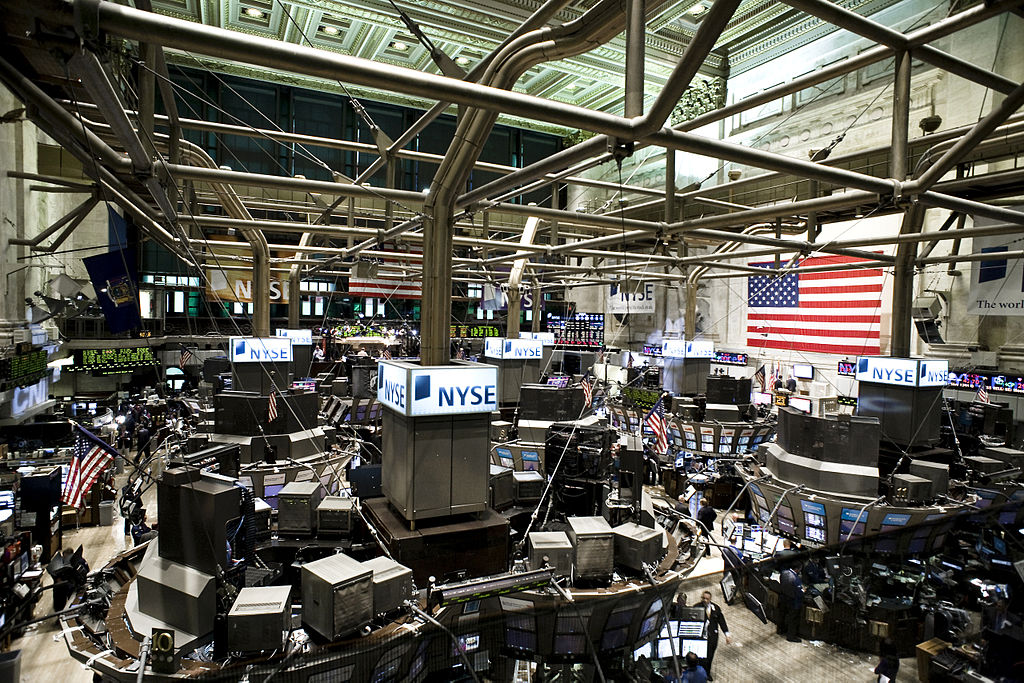
\includegraphics[width=\textwidth]{NYSE2}\\
\text{} \hfill {\color{gray} NYSE by Abhisit Vejjajiva is licensed under CC BY 2.0}
\end{center}
\vfill

The Great Recession, as it came to be called, began in 2007 when a housing bubble in the United States burst, leading to an economic decline that spread across the globe and lasted until 2009, with effects of the recession lasting even longer.  Although the causes of the recession were complicated, the root of the problem was the subprime mortgage market; thousands of people were offered mortgages to buy homes beyond what they could afford, and the true cost of the mortgages were obscured.  If they had truly known what they were getting themselves into, perhaps many of these hapless borrowers could have avoided defaulting on their mortgages and losing their homes.

The purpose of this chapter is to train you to be a careful, knowledgeable consumer.  No other area in this book will be as immediately and broadly applicable as this material on financial mathematics.  Here you'll begin to apply mathematical techniques to everyday financial management.  How much should you budget for a new car?  When should you start saving for retirement?  How is your federal income tax calculated?  These questions and ones like them will find answers in this chapter, as we investigate everything from sales taxes to credit cards.  By understanding how to manage your personal finances, you can protect yourself and take control of your financial future.
\vfill
\pagebreak

\section{Introduction}
\setcounter{ExampleCounter}{1}
\marginnote{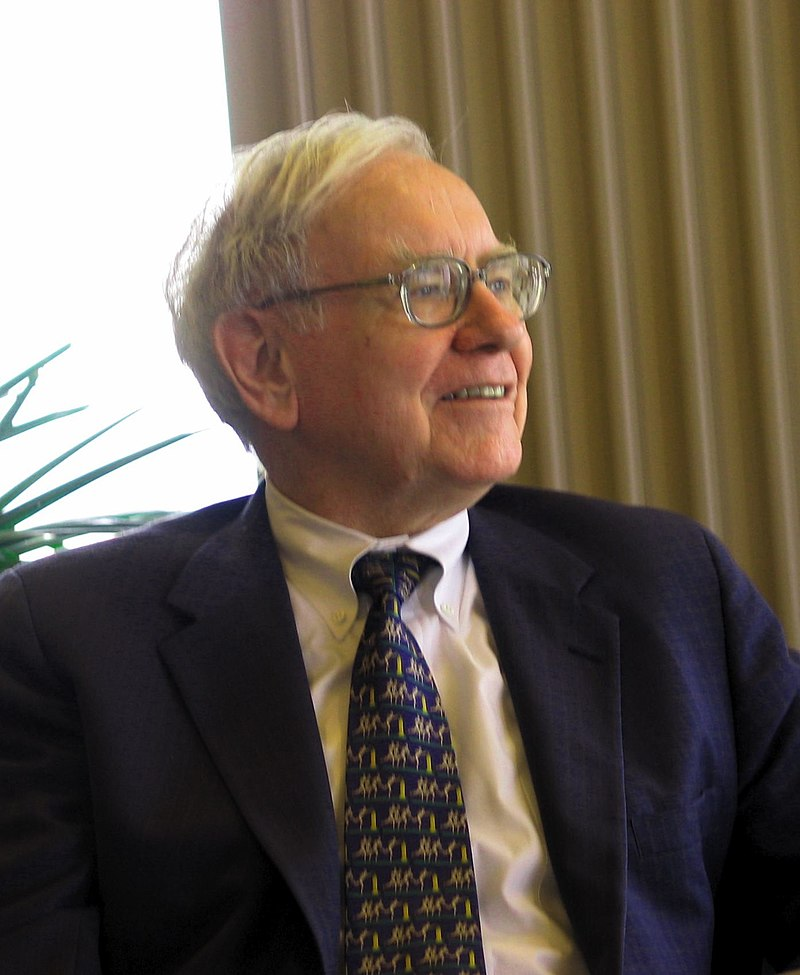
\includegraphics[width=1.5in]{WarrenBuffett}\\{\tiny\color{gray} CC BY-SA 2.0, Mark Hirschey}}
In the 1930s and 1940s, a young boy in Omaha, Nebraska spent nearly every spare hour in some entrepreneurial pursuit or another, ranging from delivering newspapers to purchasing and installing used pinball machines.  This single-minded focus on business meant that by the time he finished college, he had saved the equivalent of over \$100,000 in modern terms.

This boy, Warren Buffett, certainly benefited from some privileges, such as having the time to work and being able to keep everything he earned, but it is undeniable that his work ethic was impressive.  He didn't stop with those savings, though; through long-term investment, he parlayed those funds into one of the largest fortunes in the world (at the time of writing, Warren Buffett is the fourth-richest person in the world).  The ``Oracle of Omaha,'' who still lives in the home that he bought in 1957 for \$31,500, has pledged to give away 99\% of his vast fortune to charity.

Why do we begin with this story?  There are many other investors who were not so fortunate, but Warren Buffett is a dramatic example of the old adage, ``It takes money to make money.''  One of the most notable things about Buffett is his frugality; rather than spending his money, he has spent decades re-investing it.  Perhaps we could rephrase the adage in a slightly less pithy way:
\begin{center}
Money is expected to grow over time.
\end{center}

Take a look, for instance, at a graph of the Dow Jones Industrial Average over the past 30 years.  The DJIA is a value calculated by adjusting the sum of the prices of the stocks for thirty major companies such as Coca-Cola, Nike, Microsoft, and Walmart.  It can be used to give a quick snapshot of how the stock market in general is behaving.
\begin{center}
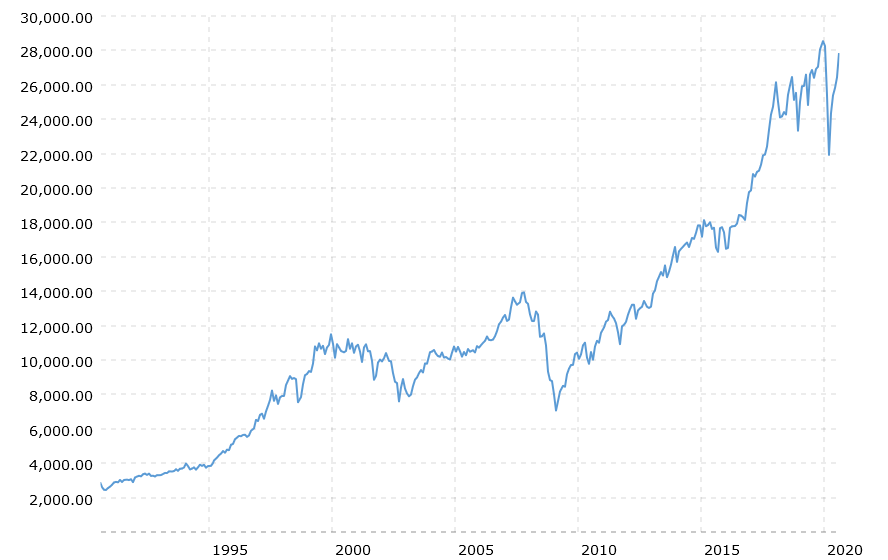
\includegraphics[width=0.8\textwidth]{DowJones}\\
\text{} \hfill {\color{gray} Source: Macrotrends.net}
\end{center}

The value of the Dow Jones index is fairly volatile, and there are notable dips (notice the big drop in 2007, when the Great Recession began, and how the graph began to creep up again in 2009, as the recession eased).  However, the overall trend is unmistakable: if you zoom out, the value of the stock market has increased steadily, and is expected to continue growing, even if there are short-term drops.

\subsection{Time Value of Money}
Let's take a smaller-scale example.  Suppose you want to start a small business; let's say for the sake of argument that you'll be starting a landscaping company.  You immediately run into a problem, though: if you had all the equipment you needed, you'd be able to start making money right away by offering your services.  However, you don't have everything you need.  You'll need a truck and a trailer, mowers and other equipment, and some form of advertising (business cards, signs, a website, etc.).  What you've run into is that same principle: ``It takes money to make money.''  If you had the money to start your business, you could invest in your landscaping company and use that to make more money.

So what do you do?  The solution is to go to a bank and take out a small-business loan, because the bank has the cash on hand, and they recognize that if they loan it to you, you'll be able to---through your hard work---multiply that money several times over, so you'll be able to repay them.

This is the foundation of the principle that we expect money to grow over time.  If you have some money today beyond what you need to cover living expenses, you can find some way to use it---either by adding your own hard work to it or finding somebody else who can do that---and by using it wisely, you can receive back more than you put in.

\begin{formula}{Time Value of Money}
\begin{center}
\marginnote{``Money is of the prolific, generating nature.  Money can beget money, and its offspring can beget more, and so on.''\\
\text{} \hfill -Benjamin Franklin}
Money is expected to grow over time.
\end{center}
We'll have specific formulas for this later, but for now, all we need is the basic principle.  For instance, \$100 today may be expected to be worth \$110 a year from now.  In this example, the \textbf{present value} is \$100, and the \textbf{future value} is \$110.
\end{formula}

Since this is the basis of the entire economy, we can simplify the big picture by envisioning money as something that grows.  There are many implications of this, but the most significant one is this: there is value to holding money right now.  Because of that, if you want to borrow money, you not only have to pay it back at some point, but you also have to pay extra on top of that for the privilege of holding onto the money for some time--this brings us to the crucial concept of \textbf{interest}.

Think back to the example of the landscaping company: you go to the bank and take out a small-business loan.  When you do, they will lay out the terms of the loan.  For instance, say you take out a loan of \$100,000 for 10 years.  That means that by the end of the 10 years, you'll have to pay back all of the original \$100,000, plus whatever interest the bank adds on top.  The question of \textbf{how} you pay it back, whether in one lump sum at the end or in smaller regular payments, will be addressed in later sections of this chapter.

\begin{formula}{Loans}
Here are a few terms that will be used frequently throughout the chapter:
\begin{itemize}
\item \textbf{Principal}: The amount of money borrowed
\item \textbf{Interest}: The fee added to the principal, which must also be paid
\item \textbf{Life of the loan}: The amount of time until the loan must be paid off
\end{itemize}
\end{formula}

In the example above, the principal is \$100,000 and the life of the loan is 10 years.\\

What about the interest?

\subsection{Interest Rates}
We need a fair way to decide how much interest to charge for a particular loan.  Let's start with a simple example.

Pretend that you are in the bank's position: you have money to loan out, and you're accepting loan applications.  Two people send in applications:
\begin{itemize}
\item One requests \$100,000 to buy a foreclosed house, fix it up, and resell it
\item The other requests \$500,000 to buy 5 foreclosed houses, fix them all up, and resell them
\end{itemize}
How much do you charge them in interest?

Clearly it wouldn't make sense to charge a flat rate.  Since both are making the same investment, but the second person is doing five times as much as the first, it's reasonable to assume that they will also see about five times the return as the first person.

Therefore, \textbf{interest scales with the amount of the loan}.  This means that interest is always a fraction of the principal, although interest rates are described using percentages.

\begin{formula}{Interest Rates}
Interest is always defined as a percentage of the principal.
\end{formula}

For instance, if you take out a loan of \$100 for a year and agree to pay 5\% interest, that means that at the end of the year you will owe \$100 plus 5\% of \$100.

This means that we need to be comfortable working with percentages before we can solve the problems later in this chapter.  Because of this, we'll include a short discussion of percentages here.  More examples can be found in the review chapter included at the end of the book, and the next section will cover applied problems that use percentages.

\subsection{Percentages}
\marginnote{\textbf{Percent:} \\ number of hundredths}
A percentage is simply another way to represent a fraction or a decimal.  The word ``percent'' means ``per 100,'' or ``number of hundredths.''

\begin{proc}{Percents, Fractions, and Decimals}
Since percent (\%) means ``number of hundredths,'' we can convert decimals to percents by multiplying by 100 (or moving the decimal point two places to the right).\\

We can convert fractions to percents the same way by first writing them as decimals.
\end{proc}

\begin{example}[https://www.youtube.com/watch?v=UZHLvEmFrOk&list=PLfmpjsIzhztsZtnb7HnXrQ8SLoiOCIcAM&index=1]{Converting to Percentages}
Convert each of the following to a percentage:\\

\begin{tabular}{l l l}
(a) $\dfrac{2}{5}$ & (b) $0.15$ & (c) $\dfrac{9}{2}$
\end{tabular}

\sol
\begin{center}
\begin{tabular}{l l l}
(a) $\dfrac{2}{5} = 0.40 = 40\%$ & (b) $0.15 = 15\%$ & (c) $\dfrac{9}{2} = 4.50 = 450\%$
\end{tabular}
\end{center}
\end{example}

\begin{try}[http://hartleymath.com/versatilemath/tryit/\#/financial-mathematics--converting-to-percentages]
Convert each of the following to a percentage:\\

\begin{tabular}{l l l}
(a) $\dfrac{3}{5}$ & (b) $0.7$ & (c) 2
\end{tabular}
\end{try}

This process can be reversed to convert a percentage to a decimal, which we'll want to do frequently in later sections of this chapter.

To do so, simply remove the percent symbol and divide the percentage by 100 (i.e. move the decimal point two places to the left).
%\vfill
%\pagebreak

\begin{example}[https://www.youtube.com/watch?v=d770dB9RHIc&list=PLfmpjsIzhztsZtnb7HnXrQ8SLoiOCIcAM&index=2]{Converting Percents to Decimals}
Convert the following percentages to decimals:\\

\begin{tabular}{l l l}
(a) 28\% & (b) 104\% & (c) 0.37\%
\end{tabular}

\sol
\begin{center}
\begin{tabular}{l l l}
(a) $28\% = 0.28$ & (b) $104\% = 1.04$ & (c) $0.37\% = 0.0037$
\end{tabular}
\end{center}
\end{example}
\pagebreak

\subsection{What's Coming Next}
With that, we're ready to dive into the rest of the chapter and explore all kinds of financial concepts.  The most important principle that you need to carry with you is the simple idea we've seen several times: money is expected to grow over time, so whenever someone borrows money, the lender expects to not only get the principal back, but also some percentage in interest.  The same concept applies when you put money into a bank account or other investment: you can expect to receive interest as payment for that account holding your money.

Here's what to expect in the rest of the chapter:
\paragraph{Section 1.2: Applied Percentage Problems} Solve word problems that involve percentages, like ``If a \$20 shirt is discounted by 15\%, what's the sale price?''

\paragraph{Section 1.3: Simple and Compound Interest} Learn about compound interest and how it makes investments grow with incredible speed.

\paragraph{Section 1.4: Saving for Retirement} It may seem far away now, but if you learn nothing else from this chapter, remember this: start saving for retirement \textbf{now}, even if you can only afford to save a little at a time.

\paragraph{Section 1.5: Mortgages and Credit Cards} Car payments, home mortgages, and credit cards are all examples of \textit{installment loans}, which are paid back with regular payments.

\paragraph{Section 1.6: Income Tax} The endlessly quotable Benjamin Franklin famously said, ``In this world nothing can be said to be certain, except death and taxes.''  Learn the basics of how income tax is calculated.
\vfill
\pagebreak

\section{Applied Percentage Problems}
\setcounter{ExampleCounter}{1}
In 1804, Thomas Jefferson won the U.S. presidential election, edging out Charles C. Pinckney by 65,191 votes.  A little over 100 years later, in the 1908 election, William Howard Taft beat William Jennings Bryan by 1,269,356 votes.  The question is, who had a wider margin of victory?
\begin{center}
\begin{tabular}{c c c}
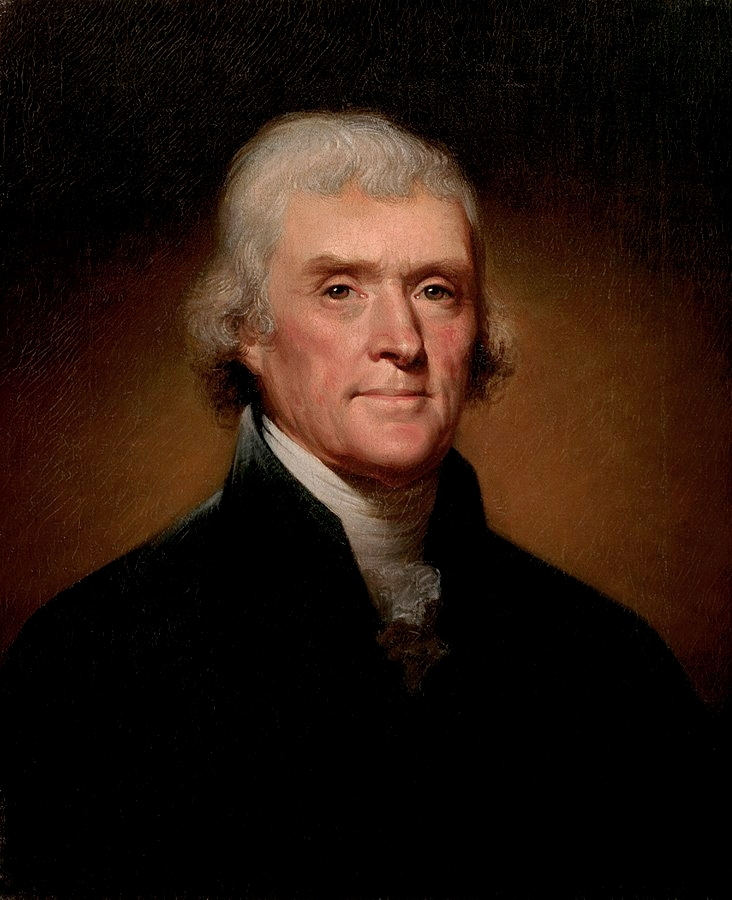
\includegraphics[height=2in]{ThomasJefferson} & \text{} \hspace*{1in} \text{} & 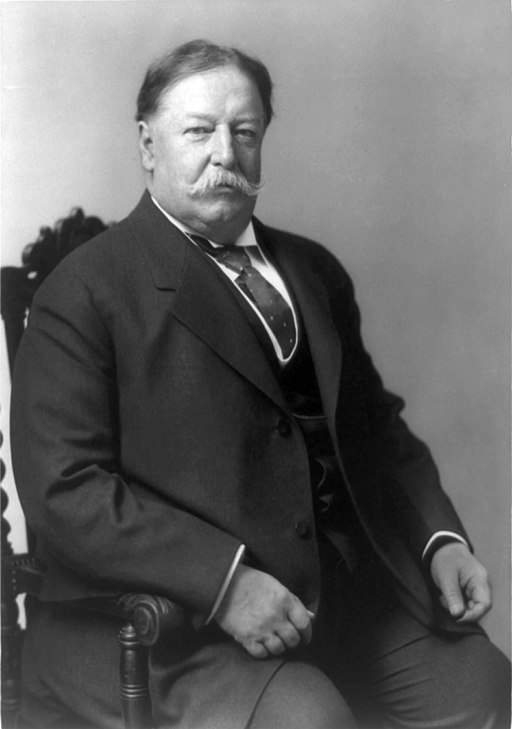
\includegraphics[height=2in]{WilliamTaft}\\
{\color{gray}Thomas Jefferson} & & {\color{gray}William Howard Taft}
\end{tabular}
\end{center}

Although Taft won his election by more votes than Jefferson, you've probably already spotted why this is misleading on its own: there were more votes cast in 1908 than in 1804.  In order to compare these two values fairly, we need more information; specifically, we need to know how many votes were counted in total each year.

There were only 143,029 total votes in 1804, compared to 14,889,239 in 1908.  We need a way to scale the margins of victory based on these totals; to do this, we can find what \textbf{percentage} of the total votes is represented by the margin.

\paragraph{Jefferson} \[\dfrac{65,191}{143,029}=0.456=\scalebox{1.7}{45.6\%}\]

\paragraph{Taft} \[\dfrac{1,269,356}{14,889,239}=0.085=\scalebox{1.7}{8.5\%}\]

By putting both numbers in context, we can tell that Jefferson won by a historic margin; the \textit{difference} between him and his opponent was nearly half of all voters, and he won over 70\% of all votes.  Although Taft still won by a fairly large percentage, it was nowhere close to Jefferson's win.

\begin{formula}{Why Use Percentages?}
Percentages are used to add context to a number, and to scale numbers so that they can be compared.
\end{formula}
\pagebreak

Percentages give us a consistent way to scale numbers.  This is important because it's often hard for us to put numbers--especially large numbers--in context.  For instance, a few years ago, an ad for an accounting firm claimed that Americans left a billion dollars behind by not getting the most out of their tax refunds, and they punctuated this with dramatic visuals of dropping pallets of cash.

\begin{center}
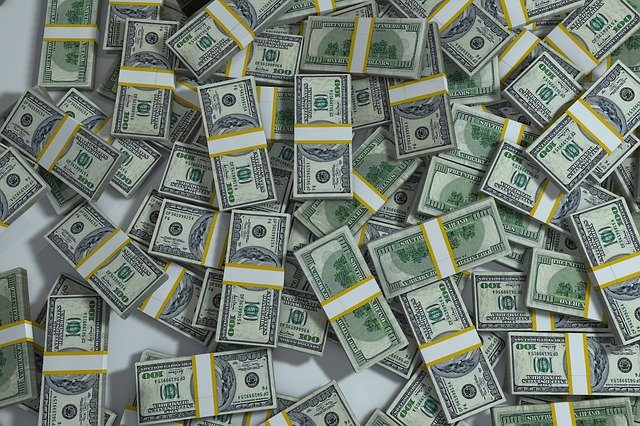
\includegraphics[width=0.4\textwidth]{cashStack}
\end{center}

For us as individuals, \$1,000,000,000 is certainly an eye-catching number, but that ad was trying to take advantage of how difficult it is to comprehend such large numbers.  Once again, though, we can put this amount in context by asking the question, ``What percentage is this of all taxes that were paid?''

In 2019, the U.S. federal government collected a total of \$3.5 trillion.  If we divide \$1 billion by this total, we find out that the billion dollars represents less than 0.03\% of all taxes collected, which is completely insignificant.

It turns out that there's an added benefit to calculating this percentage.  Once we know that number, we can use it to estimate how much an individual ``left behind,'' to borrow the terminology of the ad.  If someone paid \$10,000 in federal taxes, for instance, we can calculate 0.03\% of \$10,000.  We'll discuss how to do this more later, but it turns out that this is a grand total of\ldots around \$3.

Is that significant?  Maybe, or maybe not, but remember that this was part of an ad designed to sell accounting services, and it seems unlikely they'd charge less than \$3 for their services.

\subsection{Word Problems with Percentages}
Consider the following three questions.  You don't need to solve them yet; just look at their structure.
\begin{itemize}
\item What is 20\% of 275?
\item Eighteen is what percentage of 54?
\item Twelve is 45.3\% of what?
\end{itemize}

Do you notice any similarities?  If you look carefully, you should see a common structure.

\begin{formula}{Applied Percentage Problems}
Every applied percentage problem can be written in the following form:
\begin{center}
$A$ is $P$ percent of $B$
\end{center}
Remember that when translating a sentence into its mathematical form, the word ``is'' gets replaced with the equals sign (since ``is'' really means ``this thing and that thing are equal''), and the word ``of'' gets replaced with multiplication.

This means that every percentage problem is built around the equation
\[A = PB\]
and in every problem, two of these pieces are given.  We simply have to solve for the missing piece.
\end{formula}

If you'd like, you can use the equation above every time, substituting the appropriate values each time.  The examples we started with would look like this, for instance:
\begin{itemize}
\item $A = (20\%)(275)$
\item $18 = (P)(54)$
\item $12 = (45.3\%)(B)$
\end{itemize}

However, in order to solve these problems in a more general way, we'll use $x$ to represent the unknown piece each time.  This means that for our examples, we would write
\begin{itemize}
\item $x = (20\%)(275)$
\item $18 = (x)(54)$
\item $12 = (45.3\%)(x)$
\end{itemize}

The reason for this is that once you get used to translating a word problem into its mathematical form and replacing the unknown with $x$, you can take that process and apply it to other kinds of problems.

\begin{proc}{Percentages or Decimals?}
Remember that a percentage is simply another way to express a decimal or fraction (50\% is the same as 0.5, which is also the same as 1/2).

It's important to remember that percentages are just meant for displaying numbers, not for doing calculations.

\begin{center}
\textbf{When doing calculations, always use the decimal form of a percentage.}
\end{center}

As you'll see in many of the examples to follow, we'll give answers in both decimal form and percentage form, so you should be comfortable converting back and forth.  It's common to give an answer in the same form as the problem is given, though, so if someone asks you a question about a percentage, you should give your answer as a percentage, even though you'll use decimals during the calculation phase.
\end{proc}

\begin{example}[https://www.youtube.com/watch?v=CiMr5erFgpE&list=PLfmpjsIzhztsZtnb7HnXrQ8SLoiOCIcAM&index=3]{Setting up Percentage Questions}
Answer each of the following questions:
\begin{enumerate}[(a)]
\item What is 75\% of 690?
\item Forty is what percentage of 150?
\item Eight is 62\% of what?
\end{enumerate}

\sol
Just like we did at the start of the section, we'll start by rewriting each of these as an equation, with $x$ in place of the word ``what.''  Then we simply need to solve for $x$; be careful, though, to note whether $x$ represents a percentage or not, so that we know how to phrase the answer.

\begin{enumerate}[(a)]
\item What is 75\% of 690?
\[x = (75\%)(690)\]
This equation is already solved for us, in the sense that $x$ is already alone on one side; all that we have to do is calculate 75\% times 690, and we're done.  However, we need to remember:
\begin{center}
\textbf{When doing calculations, always use the decimal form of a percentage.}
\end{center}
That means that we need to rewrite 75\% as a decimal; remember that to do this, we simply divide 75 by 100 (or drop the percentage symbol and move the decimal place two places to the left).
\begin{align*}
75\% &= \dfrac{75}{100} = 0.75\\
x &= (0.75)(690)\\
&= \boxed{517.5}
\end{align*}
\pagebreak

\item Forty is what percentage of 150?
\[40 = (x)(150)\]
To solve for $x$, we need to get rid of the 150 that is multiplied with it; we do this by dividing both sides by 150:
\begin{align*}
40 &= (x)(150)\\
\dfrac{40}{150} &= x\\
0.2667 &= x
\end{align*}
Notice that at the end of the calculation, we have the answer as a decimal, but since the question asked ``what \emph{percentage}...'' we should give the answer as a percentage (multiply by 100 and add the percentage symbol):
\[x = \boxed{26.67\%}\]

\item Eight is 62\% of what?
\[8 = (62\%)(x)\]
Again, start by rewriting 62\% as a decimal, then solve for $x$ by dividing both sides of the equation by the result.
\begin{align*}
8 &= (0.62)(x)\\
\dfrac{8}{0.62} &= x\\
\boxed{12.9} &= x
\end{align*}
\end{enumerate}
\end{example}

\begin{try}[http://hartleymath.com/versatilemath/tryit/\#/financial-mathematics--setting-up-applied-percentage-questions]
Answer each of the following questions:
\begin{enumerate}[(a)]
\item What is 20\% of 275?
\item Eighteen is what percentage of 54?
\item Twelve is 45.3\% of what?
\end{enumerate}
\end{try}

Here's the good news: if you can do those three examples, there's no problem in this section you can't solve.  Every single word problem involving percentages follows the pattern of one of those three; all you have to do is figure out which pattern it is.\\

For instance, if you find that you paid \$4000 in federal income tax one year on a salary of \$45,662, you can figure out your \emph{effective tax rate}, meaning what percentage of your income went to income tax.  Just rephrase this in the standard form; what you really want to know is
\begin{center}
\$4000 is what percentage of \$45,662?
\end{center}
Once you see it in that form, you can run through the same steps as the last example, and you'll soon see that to get the answer, you'll need to divide \$4000 by \$45,662.

It may be that you eventually get to the point where you can simply get used to jumping to that step and skipping the rest of the process.  If you do, feel free to do so, but if you're not comfortable skipping steps, you can always deliberately set up the problem in this standard form.
\vfill
\pagebreak

\begin{example}[https://www.youtube.com/watch?v=8VSRt2PMqJI&list=PLfmpjsIzhztsZtnb7HnXrQ8SLoiOCIcAM&index=4]{Coffee Survey}
The Frederick News Post did a poll of 1500 people, asking them the following question: ``Do you go to Starbucks at least 3 times a week?'' Of those 1500 polled, 58\% said yes.  How many people replied yes to the survey?

\sol
The goal is to rephrase this question in a familiar form, along the lines of 
\begin{center}
$A$ is $P$ percent of $B$
\end{center}
and figure out where the ``what'' goes (which part of the problem is unknown).\\

We know there are a total of 1500 people surveyed, and we know that \textbf{of} that total, 58\% responded yes.  This means that our question looks like
\begin{center}
What is 58\% of 1500?
\end{center}

If we replace ``is'' with the equals sign and ``of'' with multiplication, we get the following equation:
\begin{align*}
x &= (58\%)(1500)\\
&= (0.58)(1500)\\
&= \boxed{870}
\end{align*}

Thus, 870 people responded yes to the survey.
\end{example}

\begin{try}[http://hartleymath.com/versatilemath/tryit/\#/financial-mathematics--percentage-of-female-students]
If there are 6,233 students enrolled this semester, and 59\% of those are women, how many women are attending the college this semester?
\end{try}

Let's try one with the shortcut: rather than setting up the full equation and solving for $x$, remember that if we're looking for a percentage, it's going to be one number divided by the other.  Here's the trick: if you can't figure out which order to use for division, try one and see if your answer is on the right side of 100\%.

In other words, say your question is ``Five is what percentage of 10?''  If you divide 10 by 5, you get 10/5 = 2, which is equal to 200\%.  Since this is greater than 100\%, this answer claims that 5 is greater than 10, so clearly that's the wrong order for division.  If we go back and divide 5 by 10, we'll get the correct answer.

Of course, after you do this a few times, you'll get used to the idea that the number by itself on one side of the ``is'' gets divided by the number that's mentioned with the percentage.

\begin{example}[https://www.youtube.com/watch?v=C8SnqyhsVeo&list=PLfmpjsIzhztsZtnb7HnXrQ8SLoiOCIcAM&index=5]{Dog People}
\marginnote{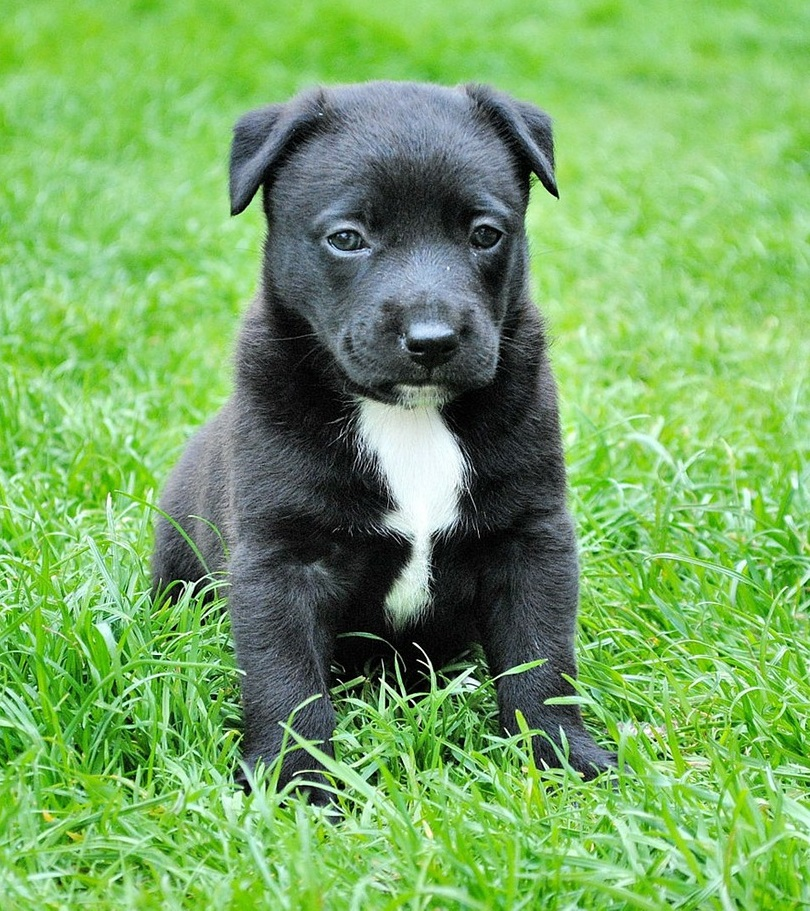
\includegraphics[scale=0.15]{Puppy1}}
In a survey of 400 people, 243 responded that they like dogs.  What percentage of these people like dogs?

\solline

Let's try the shortcut method here.  The question can be rephrased ``What percentage of 400 is 243?''  We know, since we're looking for the percentage, that we need to divide these two numbers, but the only question is what order to use for the division.\\

If we divide 400 by 243, we'll get a number larger than 1, or a percentage greater than 100\%, which can't be right, so we need to divide 243 by 400:

\[=\dfrac{243}{400} = 0.6075 = \boxed{60.75\%}\]

Roughly 61\% of people responded that they like dogs.
\end{example}

\begin{try}[http://hartleymath.com/versatilemath/tryit/\#/financial-mathematics--female-supreme-court-justices]
Three of the nine sitting members of the U.S. Supreme Court are female.  What percentage of the court is comprised of women?
\end{try}
\pagebreak

\text{}
\vfill

\begin{proc}{Tips for Percentage Problems}
In the standard problem
\begin{center}
$A$ is $P$ percent of $B$
\end{center}
there are three possibilities for what to solve for: $A$, $P$, and $B$.
\begin{itemize}
\item To solve for the percentage $P$, you'll always need to divide one of the given numbers by the other.  To find the order of division, think about whether the answer should be greater than or less than 1 (or 100\%).  If it should be greater than 1, divide the larger number by the smaller one, and vice versa.
\begin{itemize}
\item \textbf{Note:} the number by itself on one side of the word ``is'' will be divided by the other
\end{itemize}
\item If the percentage is given, and the goal is to find $A$ or $B$, you'll need to either multiply or divide the given number by the percentage that's given.  Which one you do depends on which number you're given:
\begin{itemize}
\item If you know the number that's linked to the percentage by the word ``of,'' multiply, since ``of'' is equivalent to multiplication.
\item Otherwise, divide the given number by the percentage.
\end{itemize}
\end{itemize}
\end{proc}
\vfill

\begin{example}[https://www.youtube.com/watch?v=yCQCFHGGHms&list=PLfmpjsIzhztsZtnb7HnXrQ8SLoiOCIcAM&index=6]{Sales Tax}
Suppose that you load a grocery cart with \$159 worth of groceries, and the local sales tax rate is 7\%. How much tax do you pay, and what is the total cost of the groceries?\\

\sol
The sales tax rate tells you what percentage of the price will be added on top, so we'll calculate 7\% of \$159 and add that to \$159:
\begin{align*}
(\$159)(7\%) = (\$159)(0.07) &= \$11.13\\
&+ \$159 = \boxed{\$170.13}
\end{align*}

\marginnote{\bfseries Alternate Solution}
We could simplify the solution by noticing that we start with 100\% of the cost and add 7\% to it, so we end up with 107\% of the cost: \[(\$159)(107\%) = (\$159)(1.07) = \$170.13\]
\end{example}
\vfill

Taxes are not much fun to think about, so let's switch briefly to the happier side: discounts.  When you go to a store that advertises a sale of 30\% off, that means that whatever price is on the sticker will get slashed by 30\%.  Just like before, we can calculate the new price by finding 30\% of the sticker price and subtracting that.  Alternately, we could notice that if we're removing 30\% of the price, we'll be left with 70\% of the price.  The next example illustrates a similar situation.
\vfill
\text{}
\pagebreak

\begin{example}[https://www.youtube.com/watch?v=7s1dyRcaykU&list=PLfmpjsIzhztsZtnb7HnXrQ8SLoiOCIcAM&index=7]{Discount}
\marginnote{
\includegraphics[scale=0.1]{TV1}}
For months you have been wanting a 47'' LCD flat screen television, but the price has been too high. The store is having a one-day sale on all televisions in the store. For one day only you can take 25\% off any television. The regular price on the television
you want is \$1099.
\begin{enumerate}[(a)]
\item What is the sale price?
\item What will the final price be, including sales tax, if the sales tax rate is 8\%?
\end{enumerate}

\solline
\begin{enumerate}[(a)]
\item Since the sale takes 25\% off the top of the price, the sale price will be 75\% of the original price:
\begin{align*}
\textrm{Sale price } &= (75\%)(\$1099)\\
&= (0.75)(\$1099)\\
&= \boxed{\$824.25}
\end{align*}

\item To add the sales tax, add 8\% to this new price, so we can find 108\% of \$824.25:
\begin{align*}
\textrm{Final price } &= (108\%)(\$824.25)\\
&= (1.08)(\$824.25)\\
&= \boxed{\$890.19}
\end{align*}
\end{enumerate}
\end{example}

\begin{try}[http://hartleymath.com/versatilemath/tryit/\#/financial-mathematics--coupon-and-sales-tax]
You have a 20\% off coupon at Bed, Bath, and Beyond, and you're ready to get some new towels.  If you select some that are listed at \$30, and sales tax is 6\%, how much will your final cost be at the register?  Note that the discount is applied \textbf{before} the sales tax.
\end{try}

\paragraph{WATCH OUT!} There's a subtle pitfall lurking in the last example: you may think that since we're removing 25\% of the price for the sale, and adding 8\% for the tax, we could simple combine everything into one step and simply remove 17\% (the difference between 25\% and 8\%).

But that's not right, and if you try that calculation, you'll find that you get a different answer.  What happened?  It may be hard to spot at first, but notice that the sale is 25\% \emph{of the original price} and the tax is 8\% \emph{of the reduced price}.  Since these percentages are tied to \textbf{different} bases, they can't be combined.

This is an important idea, because this error is an easy one to see.  In fact, once you understand this, you'll likely spot this mistake in all sorts of places.

\begin{example}[https://www.youtube.com/watch?v=SOSt8uYaObc&list=PLfmpjsIzhztsZtnb7HnXrQ8SLoiOCIcAM&index=8]{A Tricky Percentage Problem}
Suppose you originally paid \$1200 in taxes.  A year later taxes decreased by 20\%, but the following year taxes increased by 20\%.  What do you pay in taxes at the end?

\sol

You may be tempted to jump to the conclusion that you'll pay \$1200 in taxes at the end, since the 20\% decrease was reversed by the 20\% increase.  Be careful, though: the decrease was 20\% of \emph{the original amount} and the increase was 20\% of \emph{the reduced amount}.  Thus, the increase was \emph{smaller} than the increase, so we expect to pay less than \$1200 at the end.\\

Specifically, after one year, the taxes would be \[(\$1200)(0.80) = \$960.\]  After two years, the taxes would be \[(\$960)(1.20) = \boxed{\$1152}\]
\end{example}

\subsection{Percentage Increase or Decrease}
There's another kind of problem involving percentages: we can talk about \textbf{percentage change}.  For instance, you might hear a presidential candidate promise to cut taxes by 12\%, or you may hear that there are 25\% more hurricanes one year than the year before.

Of course, there's no such thing as a \emph{new} percentage problem, because we know that every percentage problem has to fall into one of three categories, and we've done examples of all three.  Our only job, then, is to find how to use what we already know to solve these problems that are stated a bit differently.

The most important thing to keep in mind with a percentage change problem is that
\begin{center}
the change is given as a percentage \textbf{of the \emph{original} amount}.
\end{center}

For instance, if you knew that there were originally 400 employees at a company, and 30 of them were laid off, this means that the size of the workforce decreased by whatever percentage 30 is of 400, so the problem boils down to ``Thirty is what percentage of 400?''  Having solved several problems of that type, we know to divide 30 by 400, and that leads to the following formula.

\begin{formula}{Percentage Change}
The percentage change, or relative change, of a quantity is defined as the ratio of the total change to the original amount:
\[\textrm{Percentage Change } = \dfrac{\textrm{Total Change}}{\textrm{Original Amount}}\]
where the total change is the difference between the final and original amounts:
\[\textrm{Total Change} = \textrm{Final Amount} - \textrm{Original Amount}\]

If the percentage change is positive, the quantity increased; if it is negative, the quantity decreased.
\end{formula}

As long as you don't forget to divide by the \textbf{original amount}, not the final amount, these problems are straightforward.

\begin{example}[https://www.youtube.com/watch?v=QNzrFqGFBRA&list=PLfmpjsIzhztsZtnb7HnXrQ8SLoiOCIcAM&index=9]{Car Value}
\marginnote{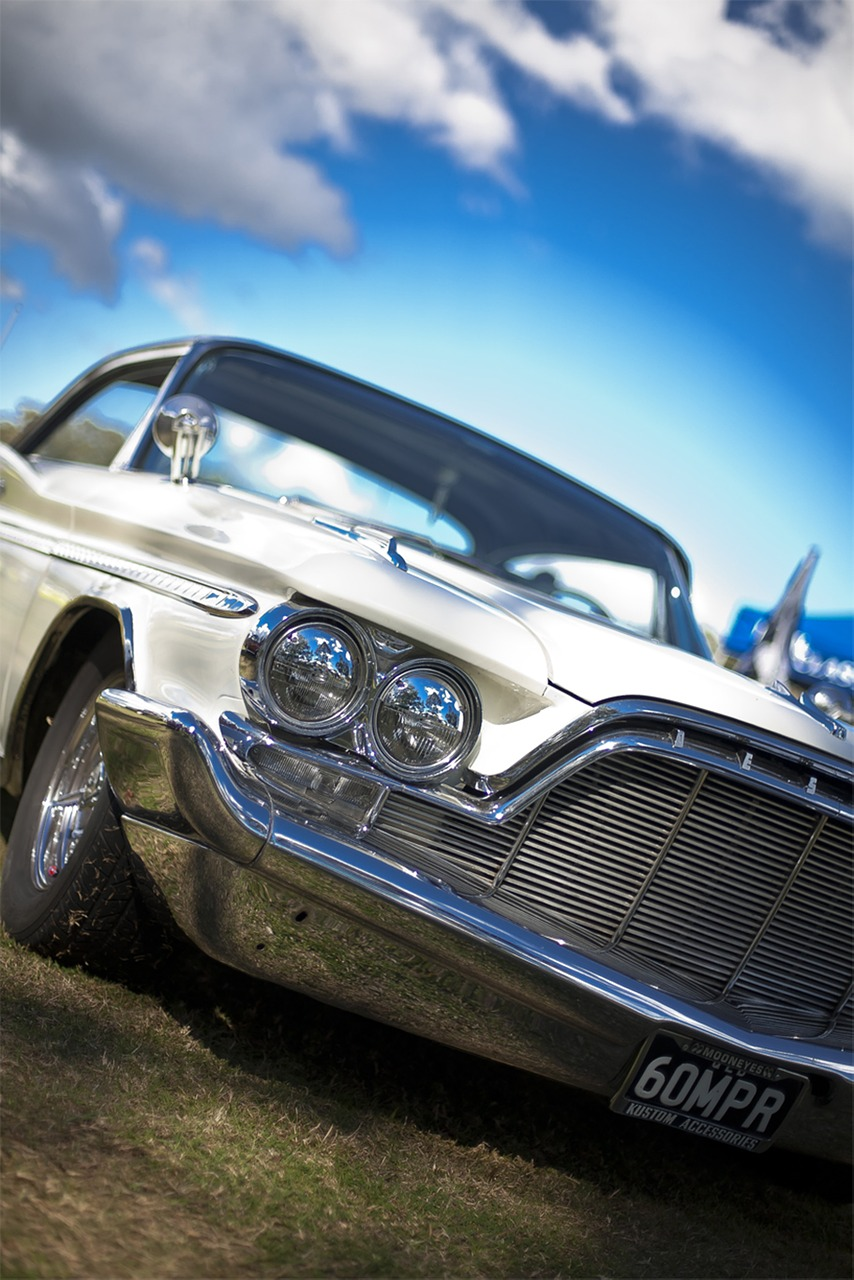
\includegraphics[scale=0.1]{Car1}}
The value of a car dropped from \$7400 to \$6800 over the last year. What percentage decrease is this?

\solline

First, find the absolute change:
\[\$7400 - \$6800 = \$600\]
Then divide this by the \textbf{original amount}:
\[\dfrac{\$600}{\$7400} = 0.081 = \boxed{8.1\%}\]

Thus, the value of the car dropped by 8.1\%.
\end{example}

\begin{try}[http://hartleymath.com/versatilemath/tryit/\#/financial-mathematics--car-dealership-discount]
You go car shopping and find your dream car for \$11,000 sitting on the lot, but unfortunately you only have \$9,000 to pay for it.  You offer the dealership the money you have and they accept your offer.  What percentage did the dealership take off the car?
\end{try}

We can also turn this kind of problem around: if we know the percentage change, we can find either the original or final amount.

If we know the original amount and the percentage change, this is exactly like the problems with discounts and sales taxes from earlier; we have a starting value and a percentage adjustment, and need to find the final amount.

Going in the other direction is a bit trickier: to find the original amount when we know the final amount and the percentage change, we need to think carefully, because the change is given as a percentage of the \emph{unknown} value.

\begin{example}[https://www.youtube.com/watch?v=gB3RqkMzDDE&list=PLfmpjsIzhztsZtnb7HnXrQ8SLoiOCIcAM&index=10]{Amount Before an Increase}
\marginnote{
\includegraphics[scale=0.08]{Books1}}
If the tuition and fees paid by the average student in the U.S. is \$9,139, and this is 17\% more than the average five years ago, what was the average cost then?

\solline

The new amount---\$9,139---is 117\% of the original cost.  Since we don't know what the original cost was, we need a placeholder for it, so we'll call it $x$:
\[\$9,139 = (117\%)(x)\]
\begin{align*}
x &= \dfrac{\$9,139}{117\%}\\
&= \dfrac{\$9,139}{1.17}\\
&= \boxed{\$7,811}
\end{align*}
The original cost, then, was \$7,811 for the average student five years ago.
\end{example}

Relative change or percent differences are also useful when comparing quantities of different sizes.  By calculating the percent difference, we can put everything on equal footing to make a meaningful comparison.

\begin{example}[https://www.youtube.com/watch?v=yQmIyPZefK0&list=PLfmpjsIzhztsZtnb7HnXrQ8SLoiOCIcAM&index=11]{Enrollment Changes}
Generally, more students go to college every semester than the semester before.  In the fall semester of 2008 there were 5,748 students enrolled at FCC; by the fall of 2009, the number had grown to 6,233.  Compare these two numbers.

\sol
We could compare them by simply finding the difference, and saying that there were 485 more students in 2009 than in 2008, but out of context this number is mostly meaningless.  At a small school like FCC, this may represent a dramatic change, but at a larger school like the author's alma mater of North Carolina State, 485 students wouldn't be as significant.\\

Instead, we can calculate this as a percentage change:
\[\dfrac{485}{5748} = 0.084 = 8.4\%\]
Enrollment rose by 8.4\%, which is a modest but respectable gain.
\end{example}

\begin{try}[http://hartleymath.com/versatilemath/tryit/\#/financial-mathematics--percentage-change-on-sat]
If you took the SAT twice, scoring 500 on the verbal portion the first time and 620 the second time, by what percentage did your score increase?
\end{try}
\pagebreak

This idea of putting different quantities on equal footing in order to compare them is extremely powerful, and crucial in many contexts.  We'll do something similar later when we consider financial applications; there, we'll be interested in, for instance, comparing two loans with different interest rates and durations and deciding which is more advantageous.  The details will differ, but the concept of finding common ground on which to compare different quantities comes up in many areas.

\begin{example}[https://www.youtube.com/watch?v=gSA_go511q4&list=PLfmpjsIzhztsZtnb7HnXrQ8SLoiOCIcAM&index=12]{Comparisons}
There are 435 Longhorn Steakhouse locations in the U.S. and 136 Ruth's Chris Steakhouse locations.  Compare these two numbers.

\sol
Rather than simply saying that there are 299 more Longhorn locations that Ruth's Chris, let's use a meaningful measure like the percentage difference.\\

We could say that Longhorn is $\frac{299}{136} = 219.9\%$ larger, or that Ruth's Chris is $\frac{299}{435} = 68.7\%$ smaller.  We could also say that Ruth's Chris is $\frac{136}{435} = 31.3\%$ of the size of Longhorn.
\end{example}

We've solved a wide array of problems using percentages, but every problem fit into one of the three categories introduced at the beginning of the section.  In the next section, we'll apply these skills to calculate how interest accrues for different kinds of loans.
\begin{exercises}
\textit{For problems 1--8, convert each number to a percent.}\\
\pfour{$\dfrac{1}{2}$}
\pfour{$0.04$}
\pfour{$\dfrac{3}{5}$}
\pfour{$0.79$}

\pfour{1.35}
\pfour{$\dfrac{10}{4}$}
\pfour{12.5}
\pfour{0.0378}

\textit{For problems 9--16, convert each percent to a decimal.}\\
\pfour{33\%}
\pfour{2.6\%}
\pfour{124\%}
\pfour{1240.5\%}

\pfour{42\%}
\pfour{4.5\%}
\pfour{0.003\%}
\pfour{$\dfrac{1}{4}\%$}

\pthree{What is 12\% of 72?}
\pthree{Ninety is what percentage of 200?}
\pthree{Twenty is 15\% of what?}

\pthree{Six is what percentage of 40?}
\pthree{Forty is 91\% of what?}
\pthree{What is 65\% of 65?}

\ptwo{In the fall of 2009 FCC enrolled 6,233 students.  Of those enrolled, 2,810 are in the 18-21 age group.  What percent of FCC students does this represent?}
\ptwo{Patrick left an \$8 tip on a \$50 restaurant bill.  What percent tip is that?}

\ptwo{Ireland has a 23\% VAT (value-added tax, similar to a sales tax).  How much will the VAT be on a purchase of a \euro 250 item?}
\ptwo{Employees in 2012 paid 4.2\% of their gross wages towards social security (FICA tax).  How much would someone earning \$45,000 a year pay toward social security?}

\ptwo{A project on Kickstarter was aiming to raise \$15,000 for a precision coffee press.  They ended up with 714 supporters, raising 557\% of their goal.  How much did they raise?}
\ptwo{Another Kickstarter project for an iPad stylus raised 1,253\% of their goal, finishing with a total of \$313,250 from 7,511 supporters.  What was their original goal?}

\ptwo{One year ago the median price for a home was \$275,000.  Now the current median price for a home is \$235,000.  What was the percent decrease in the median price of a home over the last year?}
\ptwo{There were 943 tornadoes reported in the U.S. in 2013, and 897 tornadoes were reported in 2014.  What percent decrease was there from 2013 to 2014?}

\ptwo{The population of a town increased from 3,250 in 2008 to 4,300 in 2010.  Find the absolute and percent increase.}
\ptwo{The number of CDs sold in 2010 was 114 million, down from 147 million the previous year.  Find the absolute and percent decrease.}

\ptwo{A company wants to decrease their energy use by 15\%.
\begin{enumerate}[(a)]
\item If their electric bill is currently \$2,200 a month, what will their bill be if they're successful?
\item If their next bill is \$1,700 a month, were they successful?  What percent decrease was there from the current bill?
\end{enumerate}
}
\ptwo{A store is hoping an advertising campaign will increase their number of customers by 30\%.  They currently have about 80 customers per day.
\begin{enumerate}[(a)]
\item How many customers will they have if their campaign is successful?
\item If they increase to 120 customers a day, were they successful?  What percent increase is this from the current level?
\end{enumerate}
}

\ptwo{An article reports that ``attendance dropped 6\% this year, to 300.''  What was the attendance before the drop?}
\ptwo{An article reports that ``sales have grown by 30\% this year, to \$200 million.''  What were sales before the growth?}

\ptwo{The U.S. federal debt at the end of 2001 was \$5.77 trillion, and grew to \$6.20 trillion by the end of 2002. At the end of 2005 it was \$7.91 trillion, and grew to \$8.45 trillion by the end of 2006. Calculate the absolute and relative increase for 2001-2002 and 2005-2006. Which year saw a larger relative increase in federal debt?}
\ptwo{A TV originally priced at \$799 is on sale for 30\% off. There is then a 9.2\% sales tax. Find the price after including the discount and sales tax.}

\ptwo{The Walden University had 47,456 students in 2010, while Kaplan University had 77,966 students.  Complete the following statements.
\begin{enumerate}[(a)]
\item Kaplan's enrollment was \line(1,0){20} \% larger than Walden's.
\item Walden's enrollment was \line(1,0){20} \% smaller than Kaplan's.
\item Walden's enrollment was \line(1,0){20} \% of Kaplan's.
\end{enumerate}}
\ptwo{In the 2012 Olympics, Usain Bolt ran the 100 m dash in 9.63 seconds.  Jim Hines won the 1968 gold with a time of 9.95 seconds.
\begin{enumerate}[(a)]
\item Bolt's time was \line(1,0){20} \% faster than Hines'.
\item Hines' time was \line(1,0){20} \% slower than Bolt's.
\item Hines' time was \line(1,0){20} \% of Bolt's.
\end{enumerate}}

\ptwo{A store has clearance items that have been marked down by 60\%.  They are having a sale, advertising an additional 30\% off clearance items.  What percent of the original price do you end up paying?}
\ptwo{A publisher marks up a textbook by 65\%, and a bookstore further marks up the textbook by 35\%.  What percentage of the original cost do you pay?}
\end{exercises}

\section{Simple and Compound Interest}
\setcounter{ExampleCounter}{1}
Warren Buffett, in his regular letters to his partnerships, occasionally included a section titled ``The Joys of Compounding,'' which he called ``the pulse-quickening portion of our essay.''  In one such section in a letter from 1964, he wrote about the \emph{Mona Lisa}:
\marginnote{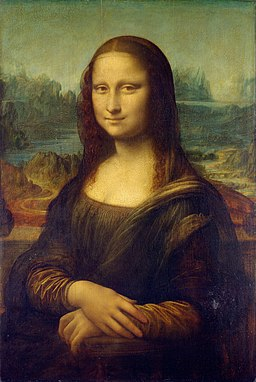
\includegraphics[width=1.5in]{MonaLisa}}
\begin{quote}
Since the whole subject of compounding has such a crass ring to it, I will attempt to introduce a little class into the discussion by turning to the art world.  Francis I of France paid 4,000 ecus in 1540 for Leonardo da Vinci's \emph{Mona Lisa}.  On the off chance that a few of you have not kept track of the fluctuations of the ecu, 4,000 converted out to about 20,000.

If Francis had kept his feet on the ground and he (and his trustees) had been able to find a 6\% after-tax investment, the estate now would be worth something over \$1,000,000,000,000,000.00.  That's \$1 quadrillion or over 3,000 times the present national debt, all from 6\%.  I trust this will end all discussion in our household about any purchase of paintings qualifying as an investment.
\end{quote}

In a letter from the previous year, he concluded a similar example by saying
\begin{quote}
Such fanciful geometric progressions illustrate the value of either living a long time, or compounding your money at a decent rate.  I have nothing particularly helpful to say on the former point.
\end{quote}

Don't worry, though; he gives a less fanciful example, as well, showing a table like the one below, which shows the returns from a \$100,000 investment over 10, 20, and 30 years using different interest rates:
\begin{center}
\begin{tabular}{l c c c}
 & \textbf{4\%} & \textbf{8\%} & \textbf{12\%}\\
10 Years & \$48,024 & \$115,892 & \$210,584\\
20 Years & \$119,111 & \$366,094 & \$864,627\\
30 Years & \$224,337 & \$906,260 & \$2,895,970
\end{tabular}
\end{center}

A quick glance through this table should make the point clear: compound interest is a powerful force (there's an apocryphal quote often attributed to Albert Einstein in which he calls it the most powerful force in the universe).  Specifically, the power of compound interest comes from the length of time an investment is given to grow, and even small changes in the interest rate can have dramatic results over enough time.

By the way, although you won't find a bank account that offers interest rates anything close to the ones listed above, the long-term rate of return on the stock market is around 10\%, so these values are by no means fictional.

These examples show what happens with \emph{compound interest}, but we haven't yet discussed what that means.
\vfill

\begin{proc}{Simple and Compound Interest}
\paragraph{Simple Interest} Interest is calculated based on the principal alone (the interest rate describes what percentage of the principal is returned).\\

\paragraph{Compound Interest} The interest from one year (or month) is added to the principal, and the next year interest is calculated based on this combination of the principal and the past interest.
\end{proc}

\subsection{Simple Interest}
Suppose you take out a loan for \$500 at 10\% annual interest rate for 4 years.  Each year, (\$500)(0.1) = \$50 in interest accrues, so the total interest is 4 times this:
\[(\$500)(0.1)(4) = \$200\]
At the end of the 4 years, you'll have to pay back the principal, \$500, plus the interest, \$200, for a total of \$700, so a present value of \$500 grew to a future value of \$700.  Clearly, this growth depends on the interest rate and the amount of time involved.
\pagebreak

\text{}
\vfill

\begin{formula}{Simple Interest}
The interest, $I$, earned on a loan with principal $P$ at annual interest rate $r$ (expressed as a decimal) over a period of $t$ years is
\[I=Prt\]
This formula works with other time periods (months, for instance) as long as the interest rate is given in the same terms (so a monthly interest rate, for instance).

\paragraph{Future Value}
The future value ($F$) of this principal (or present value) $P$ is the sum of the principal and the interest:
\[F = P + Prt\]
\marginnote{Future value for simple interest}\[F = P(1+rt)\]
Other kinds of loans (like compound interest) will have different formulas for future value, but the principal is the same: this formula tells at what rate this pile of money will grow.
\end{formula}
\vfill

\paragraph{APR: Annual Percentage Rate} Note carefully that $t$ is measured in \textit{years}; this is consistent for almost all the financial formulas in this chapter.  This means that interest rates are given as \textit{annual} interest rates.  It's also possible to express loans in monthly terms.  To do so, the APR is divided into a monthly interest rate; for example, a 12\% APR would be 1\% monthly, a 6\% APR would be 0.5\% monthly, etc.
\vfill

\begin{example}{Simple Interest}
\marginnote{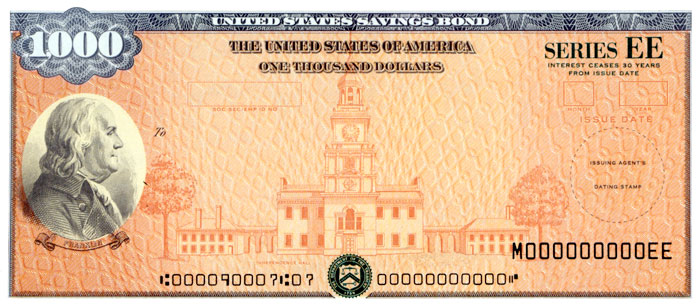
\includegraphics[scale=0.15]{TNote1}}
Treasury notes and savings bonds are issued by the federal government to cover its expenses and debt.
Suppose you obtain a \$1,000 Series EE savings bond with a 4\% annual rate and sell it 8 years later. How much interest will you earn?
\vspace{0.1in}

\sol
Use the simple interest formula above:
\begin{align*}
I &= Prt\\
&= (\$1000)(0.04)(8)\\
&= \boxed{\$320}
\end{align*}

You'll earn \$320 in interest, so at the end you'll have a total of \$1320.
\end{example}
\vfill

\begin{try}
You deposit \$3000 in a savings account at BB\&T Bank, earning 5\% interest.  Find the amount of interest earned and the total amount in the account after three years.
\end{try}

\vfill
When you're solving one of these problems, note carefully how the question is phrased.  Some may ask for the interest earned by an investment, while others may ask for the total value of the investment at the end, which is simply the principal plus the interest.

\vfill
\text{}
\pagebreak
\text{}
\vfill

\begin{example}{Future Value with Simple Interest}
If you deposit \$6200 at 6\%, what is the future value of the deposit at the end of 2.5 years?

\sol
Rather than calculating the interest first and adding that onto the principal, we can use the future value formula to do both steps at once:
\begin{align*}
F &= P(1+rt)\\
&= \$6200(1+(0.06)(2.5))\\
&= \boxed{\$7130}
\end{align*}
\end{example}
\vfill

\begin{try}
What is the future value of a \$2400 at 7\% simple interest at the end of three years?
\end{try}
\vfill

We can also turn the problem around: if we know how much we want an investment to be worth in the future, we can use a little algebra to solve for the present value, or the principal.
\vfill

\begin{example}{Present Value with Simple Interest}
You'd like to buy a \$12,000 car in 18 months, and your bank is offering 6\% simple interest.  How much should you deposit now in order to have a final balance of \$12,000?

\solline
\marginnote{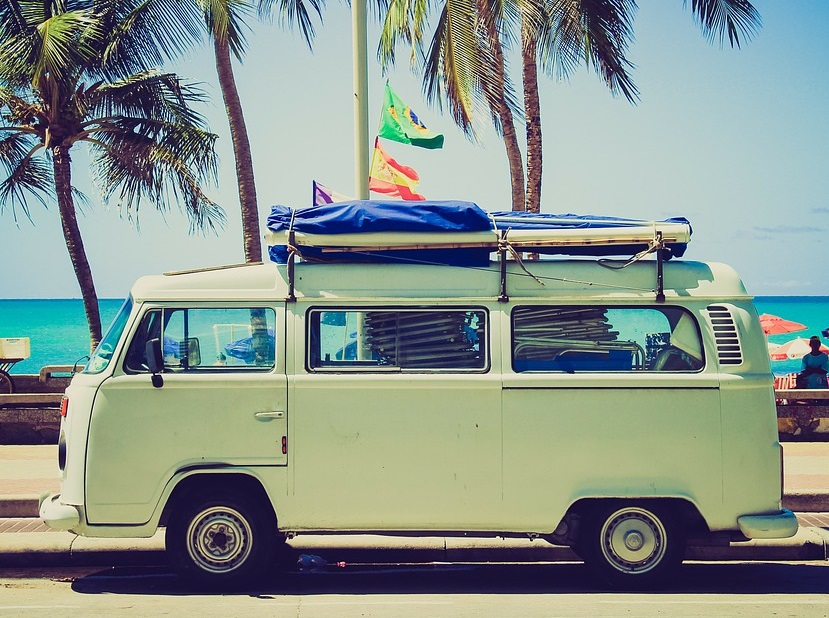
\includegraphics[scale=0.15]{VWVan1}}
We can use the same future value formula as in the previous example, but now the future value is given, and the present value is the unknown part:
\begin{align*}
F &= P(1+rt)\\
\$12,000 &= P(1+(0.06)(1.5))\\
\end{align*}

Note that $t=1.5$, since $t$ is measured in years, and 18 months is one-and-a-half years.\\

Now solve this for $P$ to find the amount that you need to deposit today:
\begin{align*}
\$12,000 &= P(1.09)\\
\dfrac{\$12,000}{1.09} &= P\\
\boxed{\$11,009.17} &= P
\end{align*}
You'll need to deposit \$11,009.17 today in order to have \$12,000 in the account in 18 months.
\end{example}
\vfill

\begin{try}
How much do you need to deposit today in an account earning 3\% simple interest to have \$800 in 36 months?
\end{try}
\vfill
\pagebreak

\subsection{Compound Interest}
With simple interest, we assumed that we pocketed the interest when we received it.  If, on the other hand, we added that interest to the account, we could earn interest on that interest in the future, making the balance grow a little bit faster.  This reinvestment of interest is called \textbf{compounding}.\\

Suppose we deposit \$5000 for 5 years in an account offering an 8\% APR, with interest compounded yearly.  How much will be in the account at the end?

At the end of each year, 8\% of the balance at that point will be added to the account, and the balance will grow.  The following table shows on a year-to-year basis the total dollar amount in the account at the end of each year and the interest that accrues that year.
\begin{center}
\begin{tabular}{| c | p{1in} | p{1.52in} | p{1.5in} |}
\hline
{\small Year} & {\small Starting Balance} & {\small Interest Earned} & {\small Final Balance}\\
\hline
1 & \$5000 & $\$5000 \times 0.08 = \$400$ & $\$5000 + \$400 = \$5400$\\
\hline
2 & \$5400 & $\$5400 \times 0.08 = \$432$ & $\$5400 + \$432 = \$5832$\\
\hline
3 & \$5832 & $\$5832 \times 0.08 = \$467$ & $\$5832 + \$467 = \$6299$\\
\hline
4 & \$6299 & $\$6299 \times 0.08 = \$504$ & $\$6299 + \$504 = \$6803$\\
\hline
5 & \$6803 & $\$6803 \times 0.08 = \$544$ & $\$6803 + \$544 = \$7347$\\
\hline
\end{tabular}
\end{center}
The total amount in the account at the end of the fifth year is \$7347, which is \$347 more than we would have earned using simple interest.

Notice that each year, the amount of interest that we earned grew, making the account grow faster and faster.  This is the advantage of compounding, and over long periods of time it can lead to very dramatic results.\\

Following this example, we can derive a formula to take care of the calculation for us so that we don't have to build a table like this every time.  At the end of the first year, the balance had grown to \[\$5000+(\$5000)(0.08) = \$5000(1+0.08).\]  Following the pattern, each year the balance is multiplied by $(1+0.08)$, so at the end of the second year, the balance grew to 
\[\$5000(1+0.08)(1+0.08) = \$5000(1+0.08)^2.\]  At the end of the third year, then, the account would hold \[\$5000(1+0.08)^3\] and so on.  

After $t$ years, the amount in an account with an interest rate of $r$, compounded once per year, will be\marginnote{Future value for interest compounded yearly} \[F=P(1+r)^t\]

\paragraph{What if interest isn't compounded yearly?} The formula we just derived assumes that interest is compounded---or added to the account---at the end of each year.  However, this doesn't have to be the case; interest could be compounded twice a year (semiannually), four times a year (quarterly), monthly, weekly, or even daily.  \marginnote{\begin{tabular}{r | l}
{\small Compounded} & $n$\\
\hline
{\small Annually} & 1\\
{\small Semiannually} & 2\\
{\small Quarterly} & 4\\
{\small Monthly} & 12\\
{\small Weekly} & 52\\
{\small Daily} & 365\footnotemark
\end{tabular}}\footnotetext{Before calculators were commonplace, some calculations used $n=360$ for daily compounding to make the arithmetic simpler} keep track of how often interest is compounded, we define $n$ as the \textbf{number of times per year that interest is compounded}, regardless of how many years the account grows.

Now if we split the year into $n$ segments, the interest rate will be divided up as well, so each segment will earn an interest rate of $\frac{r}{n}$, so that will replace $r$ in the compound interest formula.  Also, rather than having the interest accrue $t$ times, it will accrue $n$ times each year for $t$ years, or a total of $nt$ times, so that will replace $t$ in the compound interest formula.

All of this brings us to the complete formula for the future value of an investment with compound interest.
\begin{formula}{Compound Interest}
The future value $F$ of a principal amount $P$ with an annual interest rate $r$ (expressed as a decimal) compounded $n$ times per year for $t$ years is
\[F=P\left(1+\dfrac{r}{n}\right)^{nt}\]
Notice that if interest is compounded yearly, $n=1$, and the formula becomes the one we derived after the example above.
\end{formula}
\pagebreak

\begin{example}{Certificate of Deposit}
A certificate of deposit (CD) is an account that many banks offer that often comes with a higher interest rate, but the investment cannot be touched for a specified length of time.  Suppose you deposit \$3000 in a CD earning 6\% interest compounded monthly.  How much will you be able to withdraw at the end of 20 years?

\sol
List the pieces of the formula that are given:
\begin{center}
\begin{tabular}{l l}
$P$ & \$3000\\
$r$ & 0.06\\
$n$ & 12\\
$t$ & 20
\end{tabular}
\end{center}
So at the end of the 20 years, the account will hold 
\[F = 3000\left(1+\dfrac{0.06}{12}\right)^{(12)(20)} = \boxed{\$9930.61}\]

\solline
Now compare this to the amount you would earn from simple interest.
\begin{center}
\begin{tabular}{l | r | r}
Years & Simple Interest & Compound Interest\\
\hline
5 & \$3900 & \$4046.55\\
10 & \$4800 & \$5458.19\\
15 & \$5700 & \$7362.28\\
20 & \$6600 & \$9930.61\\
25 & \$7500 & \$13,394.91\\
30 & \$8400 & \$18,067.73\\
35 & \$9300 & \$24,370.65
\end{tabular}
\vspace{0.2in}

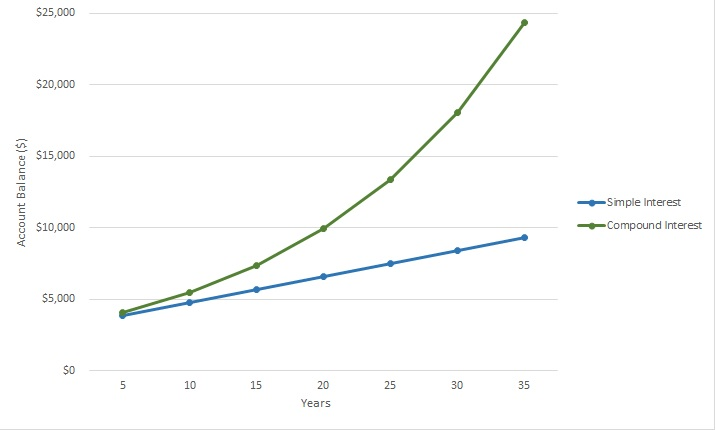
\includegraphics[scale=0.65]{SimpleCompoundGraph}
\end{center}
This illustrates the difference between the linear growth offered by simple interest and the exponential growth offered by compound interest.  Over a long period of time, compounding makes a huge difference.
\end{example}

\begin{try}
If you deposit \$700 at 5\% interest compounded monthly, how much will the account hold in 13 years?
\end{try}
\pagebreak
\text{}
\vfill

\begin{proc}{Using Your Calculator: Exponents}
\begin{tabular}{c l}
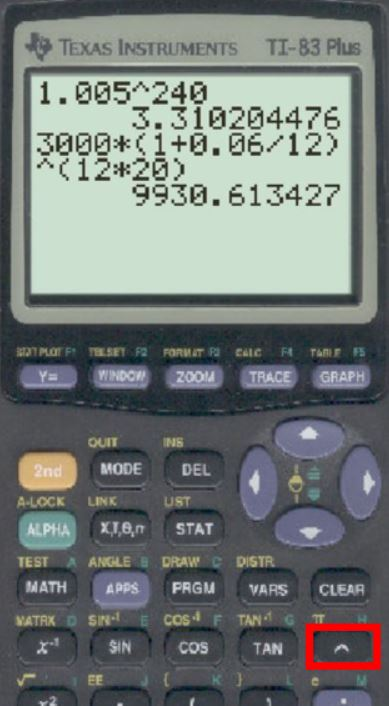
\includegraphics[scale=0.35]{Calculator1} & \parbox[b]{3in}{To evaluate an exponent like $1.005^{240}$ we use the exponent key like the one shown, or possibly $\boxed{y^x}$ or $\boxed{x^y}$ on some calculators.\\

Be careful when evaluating these often-complicated financial formulas; it's usually safer to evaluate them in pieces, like in the first line, where we began by calculating $1+0.06/12 = 1.005$ and $(12)(20)=240$, and then using the exponent key.  If you want to evaluate the entire formula in one step, be careful to use parentheses to do each operation in the proper order, as shown in the second line.\\

Also, be very careful with rounding; keep at least three significant digits (digits after leading zeros) from one calculation to the next, or use the calculator storage function.}
\end{tabular}
\end{proc}
\vfill

Just as we did with simple interest, we can also solve for present value with compound interest if we know what we want the future value to be.
\vfill

\begin{example}{Saving for College}
You know that you will need \$40,000 for your child's education in 18 years.  If your account earns 4\% compounded quarterly, how much would you need to deposit now to reach your goal?

\sol
List the pieces of the formula that are given:
\begin{center}
\begin{tabular}{l l}
$F$ & \$40,000\\
$r$ & 0.04\\
$n$ & 4\\
$t$ & 18
\end{tabular}
\end{center}
In this example, $F$ is given and $P$ is unknown:
\[40,000 = P\left(1+\dfrac{0.04}{4}\right)^{(4)(18)}\]
Solve for $P$:
\begin{align*}
P &= \dfrac{40,000}{\left(1+\dfrac{0.04}{4}\right)^{(4)(18)}}\\
&= \boxed{\$19,539.84}
\end{align*}
\end{example}
\vfill

\begin{try}
If you want to have \$26,000 in a college fund in 12 years, and you find an account earning 5\% compounded daily, how much should you deposit now?
\end{try}
\vfill
\text{}
\vfill
\pagebreak
\text{}
\vfill

\begin{proc}{Using Your Calculator: Avoid Rounding If You Can}
In many cases, you can avoid rounding to make your answers more precise based on how you use your calculator.  For example, to calculate something like
\[F = 1000\left(1+\dfrac{0.05}{12}\right)^{(12)(30)}\] start from the inside and work outward.  We can quickly calculate (maybe even mentally) that $(12)(30) = 360$, and now we can use the calculator:
\begin{center}
\begin{tabular}{c | c}
\textbf{Type This} & \textbf{Calculator Shows}\\
\hline
0.05 $\boxed{\div}$ 12 $\boxed{=}$ & 0.00416666666667\\
$\boxed{+}$ 1 $\boxed{=}$ & 1.00416666666667\\
$\boxed{y^x}$ 360 $\boxed{=}$ & 4.46774431400613\\
$\boxed{\times}$ 1000 $\boxed{=}$ & 4467.74431400613
\end{tabular}
\end{center}
\end{proc}
\vfill

\begin{example}{Don't Round Too Much}
To see why not over-rounding is so important, suppose you were investing \$1000 at 5\% compounded monthly for 30 years.
\begin{center}
\begin{tabular}{l l}
$P$ & \$3000\\
$r$ & 0.06\\
$n$ & 12\\
$t$ & 20
\end{tabular}
\end{center}
To use the formula, we'll need $\frac{r}{n}$, which is 0.0041666666666$\ldots$\\

Notice the effect of rounding this to different values:
\begin{center}
\begin{tabular}{l l l}
$r/n$ rounded: & Gives $F$ to be: & Error\\
\hline
No rounding & \$4467.74 & \\
0.0041667 & \$4467.80 & \$0.06\\
0.004167 & \$4468.28 & \$0.54\\
0.00417 & \$4473.09 & \$5.35\\
0.0042 & \$4521.45 & \$53.71\\
0.004 & \$4208.59 & \$259.15
\end{tabular}
\end{center}
Notice that the error grew by \textit{about} a factor of 10 each time, which is not unusual, considering that we rounded off a digit each time. \\

For our purposes, the answer we got by rounding to 0.004167 (four significant digits) is good enough - as long as we're not working in a bank, a rounding error of \$0.54 is fine for us.
\end{example}
\vfill
\text{}
\vfill
\pagebreak

\subsection{Comparing Interest Rates}
\begin{example}{Comparing Banks}
\marginnote{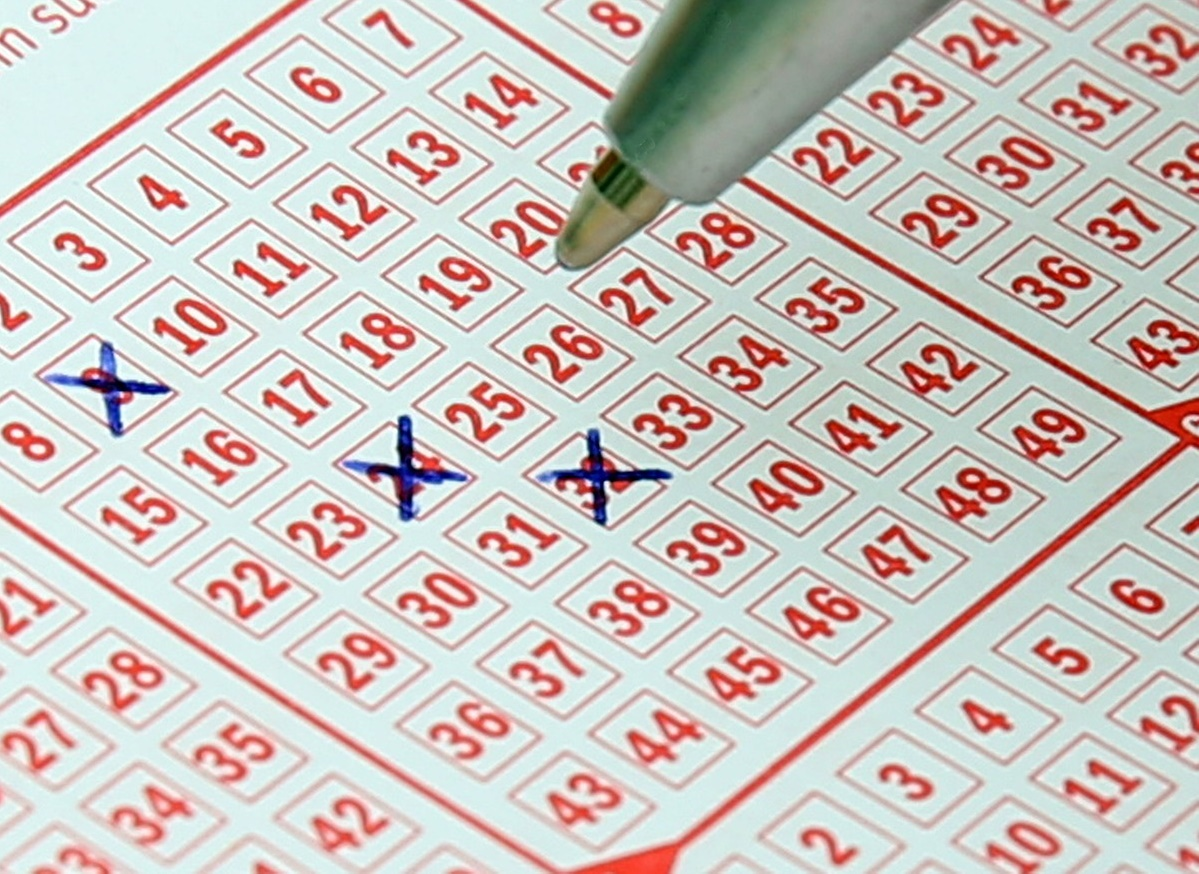
\includegraphics[scale=0.1]{Lottery1}}
You have just won \$500 in the Daily Pick 3 lottery and you decide to deposit your winnings in the bank.  You check with two different banks, which offer different options.  M\&T Bank offers a 4.25\% interest rate compounded daily, while SunTrust offers 4.3\% compounded annually.  Which bank should you choose?

\solline
To compare the two banks, simply choose an arbitrary amount of time and calculate how much each account would hold at the end of that time; whichever is higher is the one you'll choose.  Let's pick a year as our length of time, just for simplicity.  The table below shows the results of calculating the future value of your \$500 at the end of a year with each bank.
\begin{center}
\begin{tabular}{c c}
M\&T & SunTrust\\
\hline
& \\
\$521.71 & \$521.50
\end{tabular}
\end{center}
Even though the difference is relatively small, you'll choose the first account, since over time the difference may grow to something more significant.
\end{example}
\vfill

That example illustrates an important point: you'll often find different loans or accounts expressed in different terms, perhaps with different interest rates and compounding periods.  In that case, you'll want to find some way to put them all on equal footing to compare them; like we did in that example, you can often do a quick calculation to see which will earn more in some arbitrary amount of time.

Banks will often take advantage of the financial illiteracy of their clients to present a loan in terms that will subtly benefit them.  The major goal of this chapter is to turn you into a financially literate, savvy consumer.
\vfill

\begin{proc}{Sidenote: Different Interest Rates}
There are different terms you may find if you go looking for interest rates, so we'll mention a few of them here:

\paragraph{Nominal Interest Rate} The \textit{nominal interest rate} is the interest rate that is stated, such as a 3\% annual rate on a bond or a 1.7\% monthly rate on a credit card.

\paragraph{Annual Percentage Rate (APR)} This is the annual nominal rate.  So for instance, the 1.7\% nominal monthly rate would correspond to a $1.7\% \times 12 = 20.4\%$ APR.

\paragraph{Effective Interest Rate (APY)} This is the real interest rate.  The \textit{effective rate}, also called the \textit{annual percentage yield (APY)} or the \textit{effective annual yield}, takes the compounding period into account.  This is done by calculating the simple interest rate that would lead to the same growth as that of the compound interest that is offered.

\paragraph{APR vs APY} Since APY takes the effect of compounding into account and APR does not, the APY will be slightly higher than the APR for a typical account.  Because of this, banks typically report the APR for debt-related accounts like credit cards and mortgages, and they report the APY for interest-bearing accounts like CDs and money market accounts.
\end{proc}
\vfill
\text{}
\vfill
\pagebreak

\subsection{Continuously Compounded Interest}
We've seen that compound interest makes money grow faster than simple interest does, but we can go even further: if someone offered you an investment compounded monthly and one compounded daily (with everything else equal), which would you choose?  You would be wise to choose the one that is compounded daily, because the more frequently that interest is compounded, the longer that interest that is added has to grow.  In other words, the interest that is added after one day has more time to grow than if it had to wait until the end of the month to be added.

The question is this: is there a limit to this growth?  Could we compound more and more often and see our money grow infinitely?  To answer this, suppose we deposit \$1 for one year into an account with a fixed interest rate---we'll use 100\% to illustrate, even though you'll almost certainly never encounter such an interest rate in real life---and we'll see what happens as we increase $n$, the frequency with which the interest is compounded:
\begin{center}
\begin{tabular}{r r}
$n$ & \hspace{0.5in} $1\left(1+\dfrac{1}{n}\right)^n$\\
& \\
\hline
& \\
1 & 2.0000000$\ldots$\\
5 & 2.4883200$\ldots$\\
10 & 2.5937424$\ldots$\\
50 & 2.6915880$\ldots$\\
100 & 2.7048138$\ldots$\\
1000 & 2.7169239$\ldots$\\
10,000 & 2.7181459$\ldots$\\
100,000 & 2.7182682$\ldots$\\
1,000,000 & 2.7182804$\ldots$\\
10,000,000 & 2.7182816$\ldots$\\
\end{tabular}
\end{center}

Notice that as we compound more and more frequently, we start to approach a limit.  This limit happens to be a very important number, so important that the letter $e$ is reserved for it.  It forms the basis of exponential growth, which has applications in every field of applied mathematics.\\

For a general interest rate $r$, $\left(1+\dfrac{r}{n}\right)^{nt}$ approaches $e^{rt}$ as the compounding increases.  This is what we call \textit{continously compounded interest}.

\begin{formula}{Continuous Compound Interest}
A present value $P$ will grow to a future value of $F$ under continuous compounding at an interest rate of $r$ according to:
\[F = Pe^{rt}\]
\end{formula}

\begin{proc}{Using Your Calculator: $e$}
\begin{tabular}{c l}
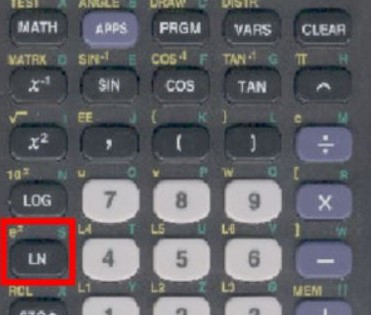
\includegraphics[scale=0.35]{CalculatorECropped} & \parbox[b]{3in}{Your calculator will most likely have a button for $e$, but depending on what kind of calculator you have, it may look different.\\

Here, the model shown has $e^x$ as the 2nd function of the button marked $\boxed{\textrm{LN}}$\ , so to calculate $e^{0.5}$, for instance, you would press $\boxed{\textrm{2nd}}$\ , then $\boxed{\textrm{LN}}$\ , then enter 0.5, and you should get 1.648721271.\\

On some scientific calculators, you may need to enter 0.5 and then press the $\boxed{e^x}$ key to get the same result.}
\end{tabular}
\end{proc}
\pagebreak

\begin{example}{Continuous Compound Interest: Future Value}
If you deposit \$4500 in an account paying 3.2\% interest compounded continuously, how much will the account hold after 36 months?

\sol
Use the continuous compound formula:
\begin{align*}
F &= Pe^{rt}\\
&= \$4500e^{(0.032)(3)}\\
&= \boxed{\$4953.42}
\end{align*}
\end{example}

\begin{try}
If you deposit \$13,000 in an account paying 2.8\% interest compounded continuously, how much will the account hold after 3 years?
\end{try}
\vfill

Once again, we can also turn the problem around and solve for the present value.
\vfill

\begin{example}{Continuous Compound Interest: Present Value}
How much will you need to deposit today at 5.3\% compounded continuously in order to have \$6300 in 4 years?

\sol
Just like before, we'll use the same formula, but now $F$ is known and $P$ is the unknown part.
\begin{align*}
F &= Pe^{rt}\\
\$6300 &= Pe^{(0.053)(4)}\\
\$6300 &= P(1.2361)\\
\dfrac{\$6300}{1.2361} &= P\\
\boxed{\$5096.48} &= P
\end{align*}
\end{example}
\vfill

\begin{try}
How much will you need to deposit today at 3.6\% compounded continuously in order to have \$1200 in 5 years?
\end{try}
\vfill
\text{}
\vfill
\pagebreak

\begin{example}{Comparing Different Compounding Periods}
You have \$7000 to invest for 5 years.  Find how much you'll have at the end of the 5 years if you earn 4\% compounded
\begin{enumerate}[(a)]
\item annually
\item monthly
\item daily
\item continuously
\end{enumerate}

\sol
The first three all use the same formula, and all that changes is $n$:
\begin{enumerate}[(a)]
\item Compounded annually:
\begin{align*}
F &= P\left(1+\dfrac{r}{n}\right)^{nt}\\
&= 7000\left(1+\dfrac{0.04}{1}\right)^{(1)(5)}\\
&= \$8516.57
\end{align*}

\item Compounded monthly:
\begin{align*}
F &= P\left(1+\dfrac{r}{n}\right)^{nt}\\
&= 7000\left(1+\dfrac{0.04}{12}\right)^{(12)(5)}\\
&= \$8546.98
\end{align*}

\item Compounded daily:
\begin{align*}
F &= P\left(1+\dfrac{r}{n}\right)^{nt}\\
&= 7000\left(1+\dfrac{0.04}{365}\right)^{(365)(5)}\\
&= \$8549.73
\end{align*}

\item Compounded continuously: \textbf{note the different formula}
\begin{align*}
F &= Pe^{rt}\\
&= 7000e^{(0.04)(5)}\\
&= \$8549.82
\end{align*}
\end{enumerate}
\end{example}

\begin{try}
If you deposit \$300, how much will you have in 7 years if you receive 3.5\% interest compounded
\begin{enumerate}[(a)]
\item quarterly?
\item monthly?
\item weekly?
\item continuously?
\end{enumerate}
\end{try}

Notice how the future value increases as interest is compounded more and more frequently.  The limit, of course, is the continuous case.
\pagebreak

\paragraph{Doubling Time} One common measure used to quickly compare investments is to determine how long it will take to double an investment.  The shorter the doubling time, the better the investment.

\begin{proc}{Solving Exponential Equations}
To solve an exponential equation, we use logarithms.  For exponential equations, we'll use the \textit{natural logarithm}, $\ln$.
\[\textrm{If } e^x = y, \textrm{ then } x = \ln y\]
\end{proc}

For more on solving equations involving exponents, see the algebra review chapter at the end of the book.

\begin{example}{Doubling Time}
Find the time required to double an investment at 6\% interest compounded continuously.\\

\sol
We could again pick an arbitrary amount for $P$, and let $F$ be double that.  Instead, though, we'll simply replace $F$ with $2P$, and solve the formula for $t$:
\begin{align*}
F &= Pe^{rt}\\
2P &= Pe^{0.06t}\\
\marginnote{note the change from exponential form to logarithmic form here}
2 &= e^{0.06t}\\
\ln 2 &= 0.06t\\
\dfrac{\ln 2}{0.06} &= t\\
\boxed{11.55} &= t
\end{align*}
Thus the investment will take approximately 11.5 years to double.
\end{example}

\begin{try}
How long will it take an investment to double at 5\% compounded continuously?
\end{try}

\begin{proc}{Doubling Time: the Rule of 72}
A quick way\marginnote{For continuous compounding, the \emph{Rule of 69.3} is more precise, but 72 is an easier number to use for mental calculations, and other compounding terms will give results closer to the Rule of 72 than continuous compounding does.} to roughly approximate doubling time is to divide 72 by the percent interest rate (i.e. not the decimal form, but 100 times that)
\[\textrm{Doubling Time } \approx \dfrac{72}{R}\]
where $R = 100r$.
\end{proc}

So for example, with an interest rate of 6\%, as in the last example, we could estimate the doubling time by dividing 72 by 6:
\[\dfrac{72}{6} = 12\]
Even though this isn't as precise as the calculation in the example, notice how much simpler it was, and knowing that our investment will double in about 12 years is just as valuable as knowing it will be precisely 11.55 years.
\pagebreak

\subsection{Using The TVM Solver}
If you have a TI-83 or TI-84 graphing calculator (or a similar model), you have a built-in application that can solve questions involving compound interest without using the formulas in this section.

Although we'll show you how to use it here, and it is possible to answer the homework questions using it, you should make sure that you can solve the problems using the formulas, just to stretch your mathematical muscles.

To begin, find the button marked $\boxed{\textrm{APPS}}$\ .  When you press that, you should have the option to select the Finance app, and when you press Enter twice, you'll enter the TVM (Time Value of Money) solver.  You should then see a screen like the following one.

\begin{center}
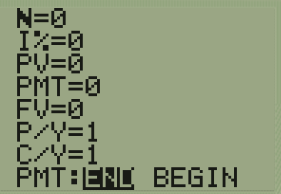
\includegraphics[width=2in]{TVMintro}
\end{center}

It's a good idea to zero out all the values at first (other than P/Y and C/Y), to make sure that you don't mistakenly use a value from another problem.

Let's go through the entries one at a time:
\begin{itemize}
\item N: the total number of compounding periods.  This means, for instance, that if interest is compounded monthly for 8 years, N would be $(12)(8) = 96$.  You could either calculate this separately, or simply type \texttt{12*8} in the space for N.  Just remember that since there's no entry for $t$, this value N is equal to $nt$ from our previous work.
\item I\%: the interest rate \textbf{as a percentage}, not a decimal.  For instance, if the interest rate is 4.5\%, simply enter 4.5 for I\%.
\item PV: the present value.  Note that the TVM solver uses the sign to indicate which direction the money is moving; cash outflow is negative, and income is positive.  If you deposit \$1000, for instance, you can enter -1000 for the present value, and the corresponding future value will be positive, since you'll recoup your investment.
\item PMT: a recurring payment.  This will come into play in the next section, but there's no need to use it for now; you can leave it as 0.
\item FV: the future value.  Again, the sign of this number will indicate which direction the money is moving.
\item P/Y: payments per year.  This too relates to the recurring payments that we'll encounter in the next section, but notice that it will always be the same as the next entry.
\item C/Y: compounding periods per year.  This is the familiar $n$ we've been using in the compound interest formula.
\end{itemize}

You can ignore the option at the end; that toggles between payments made at the beginning and end of the payment period, but we're not getting that involved.\\

The way to use this application is to enter all the information that's given, then use the SOLVE option (one of the alternate functions of the $\boxed{\textrm{ENTER}}$ key) to find the one that is unknown.  We'll illustrate with an example.
\pagebreak

\begin{example}{Using the TVM Solver}
Use the TVM solver on your calculator to find the present value needed if we want a future value of \$5000 in 6 years, if we can earn 4.3\% interest compounded monthly.

\sol
Open the TVM solver and try entering all the information that is given.  When you're done, you should see the following:
\begin{center}
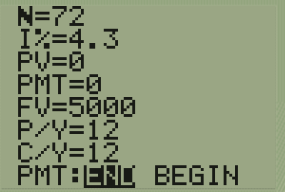
\includegraphics[width=2in]{TVMexample1}
\end{center}

Now, move the cursor to hover over the 0 next to PV=.  To access the SOLVE function on the $\boxed{\textrm{ENTER}}$ key, first press the $\boxed{\textrm{ALPHA}}$ key near the upper left corner of the keypad, then press the $\boxed{\textrm{ENTER}}$ key.

When you do, you should see the following:
\begin{center}
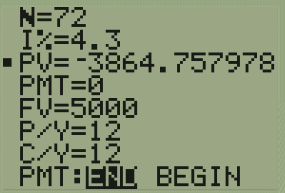
\includegraphics[width=2in]{TVMexample2}
\end{center}

Notice that the present value is given as a negative number, which indicates that if you want to receive (positive) \$5000 in the future, you need to deposit (negative) \$3864.76 now.
\end{example}

You can also use the TVM solver, for instance, to calculate the necessary interest rate if you enter both a present value and a future value.\\

Of course, there's no magic to this application; it's simply using the formulas you have already been using, and you could solve any of these problems the long way.  But it certainly is convenient to save yourself some typing.

\paragraph{Sidenote: Continuous Compounding} In case you're wondering how to handle continuous compounding, it turns out that it can be done, but it's a bit harder.

Since continuous compounding is essentially like interest compounding every instant, if we enter a huge number for C/Y, we can simulate this.  In practice, something like 1 million works well enough.  Then, let N be the number of years (so pretending that $n=1$) and let P/Y be 1, and the result will be as close as we need it to be.
\vfill
\pagebreak

\subsection{Using Excel}
Although there are some built-in formulas in Excel to calculate things like future value, it turns out that it's just as easy to create the formulas yourself and build a simple compound interest calculator.

To begin, open Microsoft Excel and enter the following labels in the first column of a worksheet:
\begin{center}
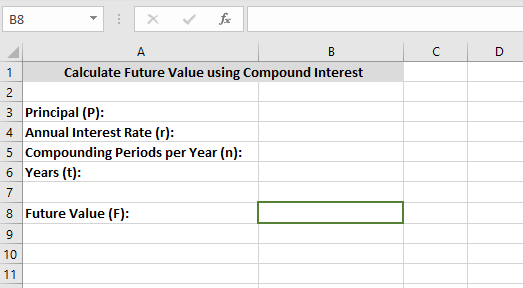
\includegraphics[width=3.5in]{ExcelExample1}
\end{center}

Notice that the highlighted cell (B8, since it is in column B and row 8) is where we want to find our answer.  We'll place the inputs in cells B3-B6:
\begin{center}
\begin{tabular}{c c}
\textbf{Value} & \textbf{Cell}\\
\hline
$P$ & B3\\
$r$ & B4\\
$n$ & B5\\
$t$ & B6
\end{tabular}
\end{center}

Thus, since the formula for $F$ is 
\[F = P\left(1+\dfrac{r}{n}\right)^{nt}\]
we can simply replace each variable with the corresponding cell in the formula we type into cell B8:
\begin{center}
Type ``\texttt{=B3*(1+B4/B5)}$\wedge$\texttt{(B5*B6)}'' into the formula box for cell B8.
\end{center}
Notice that we need to explicitly include a multiplication symbol when we want to multiply two values.
\begin{center}
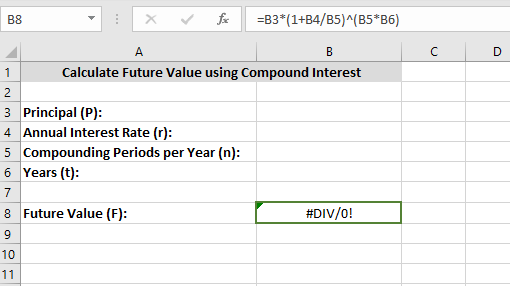
\includegraphics[width=3.5in]{ExcelExample2}
\end{center}

Notice that the result is an error at first, since we haven't filled in the other values, so the formula is forced to divide by 0, which of course isn't allowed.
\vfill
\pagebreak

Say, for instance, we want to find the future value of a \$2000 investment at 3\% for 5 years, compounded monthly.  Note that this time we'll use 0.03 for the interest rate, since the formula assumes $r$ is in decimal form.
\begin{center}
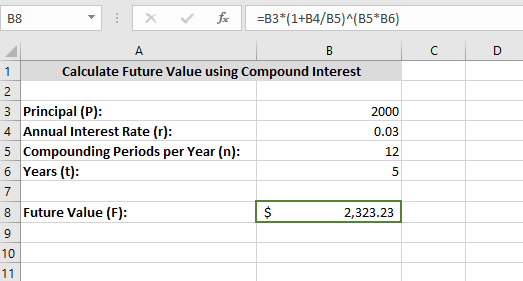
\includegraphics[width=3.5in]{ExcelExample3}
\end{center}

Notice that the output can be nicely formatted as a dollar amount by opening the Format Cells option after right-clicking on the cell.\\

There are many more ways to use Excel as a financial tool, but to calculate the result of compound interest is simple enough, using the familiar formula.
\begin{exercises}
\textit{In problems 1--3, a principal amount is borrowed at the given interest rate for the given period of time.  Find the loan's future value $F$, or the amount due at the end of the time, if the loan uses simple interest.}

\pthree{\begin{center}
\begin{tabular}{r l}
Principal: & \$3000\\
Interest rate: & 7\%\\
Time: & 2 years
\end{tabular}
\end{center}}
\pthree{\begin{center}
\begin{tabular}{r l}
Principal: & \$2700\\
Interest rate: & 4\%\\
Time: & 3 years
\end{tabular}
\end{center}}
\pthree{\begin{center}
\begin{tabular}{r l}
Principal: & \$7500\\
Interest rate: & 3.5\%\\
Time: & 18 months
\end{tabular}
\end{center}}

\textit{In problems 4--6, a principal amount is borrowed at the given interest rate for the given period of time.  If the future value is given, find the principal (present value) if the loan uses simple interest.}

\pthree{\begin{center}
\begin{tabular}{r l}
Future value: & \$9000\\
Interest rate: & 5.5\%\\
Time: & 1 year
\end{tabular}
\end{center}}
\pthree{\begin{center}
\begin{tabular}{r l}
Future value: & \$7700\\
Interest rate: & 6\%\\
Time: & 4 years
\end{tabular}
\end{center}}
\pthree{\begin{center}
\begin{tabular}{r l}
Future value: & \$800\\
Interest rate: & 2.75\%\\
Time: & 9 months
\end{tabular}
\end{center}}

\textit{In problems 7--9, a principal amount is borrowed at the given interest rate for the given period of time, and interest is compounded as stated.  Find the loan's future value $F$, or the amount due at the end of the time.}

\pthree{\begin{center}
\begin{tabular}{r l}
Principal: & \$1200\\
Interest rate: & 5\%\\
Compounding: & Annually\\
Time: & 3 years
\end{tabular}
\end{center}}
\pthree{\begin{center}
\begin{tabular}{r l}
Principal: & \$5700\\
Interest rate: & 3.5\%\\
Compounding: & Monthly\\
Time: & 24 months
\end{tabular}
\end{center}}
\pthree{\begin{center}
\begin{tabular}{r l}
Principal: & \$3000\\
Interest rate: & 5.32\%\\
Compounding: & Continuously\\
Time: & 48 months
\end{tabular}
\end{center}}

\textit{In problems 10--12, a principal amount is borrowed at the given interest rate for the given period of time, and interest is compounded as stated.  If the future value is given, find the principal.}

\pthree{\begin{center}
\begin{tabular}{r l}
Future value: & \$17,500\\
Interest rate: & 3\%\\
Compounding: & Annually\\
Time: & 8 years
\end{tabular}
\end{center}}
\pthree{\begin{center}
\begin{tabular}{r l}
Future value: & \$18,000\\
Interest rate: & 5.6\%\\
Compounding: & Daily\\
Time: & 18 months
\end{tabular}
\end{center}}
\pthree{\begin{center}
\begin{tabular}{r l}
Future value: & \$9000\\
Interest rate: & 7.48\%\\
Compounding: & Continuously\\
Time: & 60 months
\end{tabular}
\end{center}}

\ptwo{A friend lends you \$200 for a week, which you agree to repay with 5\% one-time interest. How much will you have to repay?}
\ptwo{Suppose you obtain a \$3,000 T-note with a 3\% annual rate, paid quarterly, with maturity in 5 years.  How much interest will you earn?}

\ptwo{A student took out a simple interest loan for \$2,400 for two years at an annual rate of 7\%.  
\begin{enumerate}[(a)]
\item What is the interest on the loan?
\item How much will the student have to repay at the end of two years?
\end{enumerate}
}
\ptwo{A loan of \$2,040 has been made at a 5.7\% annual simple interest rate for four months.  
\begin{enumerate}[(a)]
\item What is the interest on the loan?
\item Find the future value of the loan.
\end{enumerate}}

\ptwo{You deposit \$2000 in an account earning 3\% interest compounded monthly.
\begin{enumerate}[(a)]
\item How much will you have in the account in 20 years?
\item How much interest will you earn?
\end{enumerate}}
\ptwo{You deposit \$10,000 in an account earning 4\% interest compounded weekly.
\begin{enumerate}[(a)]
\item How much will you have in the account in 25 years?
\item How much interest will you earn?
\end{enumerate}}

\ptwo{How much would you need to deposit in an account earning 6\% compounded monthly in order to have \$6,000 in the account in 8 years?}
\ptwo{How much would you need to deposit in an account earning 5\% compounded quarterly in order to have \$20,000 in the account in 4 years?}

\ptwo{If you deposit \$5400 in an account earning 4.35\% interest compounded continuously, how much will the account hold in 18 months?}
\ptwo{If you take out a loan for \$7700 at 6.7\% interest compounded continuously, how much will you have to pay back in 5 years?}

\ptwo{How much do you need to deposit today at 4\% interest compounded continuously in order to have \$4000 in 2 years?}
\ptwo{If you find a CD offering 5.8\% interest compounded continuously, how much should you deposit if you are saving up to refinish your kitchen in 3 years and you estimate that will take \$15,000?}

\ptwo{You have \$12,000 to invest for 3 years.  Find how much you'll have at the end of the 3 years if you earn 4\% interest compounded
\begin{enumerate}[(a)]
\item annually
\item monthly
\item daily
\item continuously
\end{enumerate}}
\ptwo{You would like to have \$8000 saved in 3 years.  Find how much you'll have to invest now to reach that goal if you earn 6\% interest compounded
\begin{enumerate}[(a)]
\item annually
\item monthly
\item daily
\item continuously
\end{enumerate}}

\ptwo{How long will it take to double an investment at 7\% compounded continuously?}
\ptwo{How long will it take to double an investment at 4.6\% compounded continuously?}
\end{exercises}

\section{Saving for Retirement}
\setcounter{ExampleCounter}{1}
\begin{center}
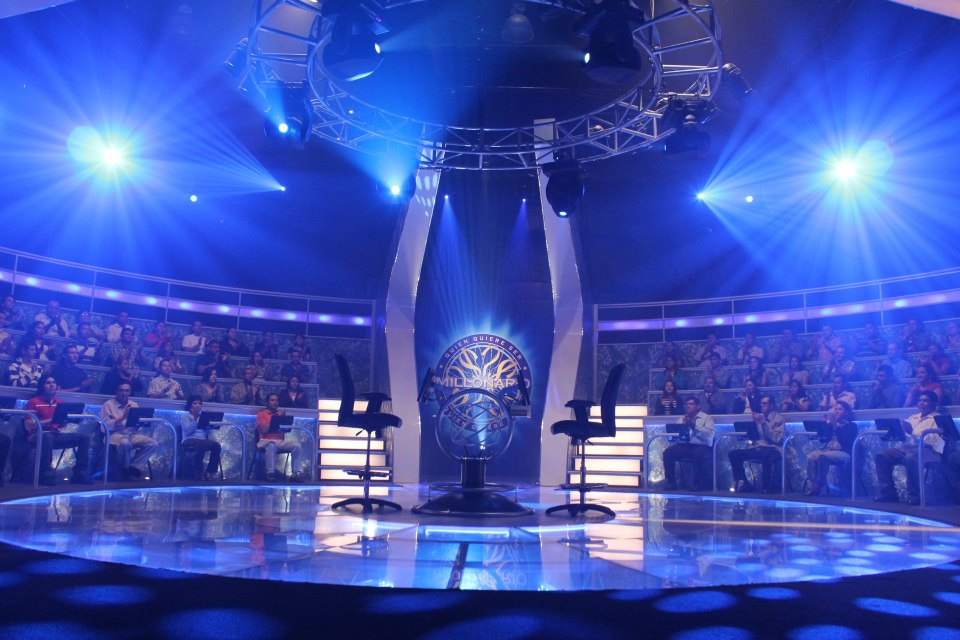
\includegraphics[width=0.8\textwidth]{Millionaire}\\
\text{} \hfill {\color{gray}Image by Wikipedia user Idea SV is licensed under CC BY-SA 3.0}
\end{center}

Who wants to be a millionaire?  More realistically, who \emph{doesn't} want to be a millionaire?  It may sound like an unattainable goal, but in this section, you'll learn how you can join the millionaire club by taking advantage of the power of compound interest.

If you forget everything else you learn here, don't forget this one lesson:
\begin{center}
{\LARGE START SAVING EARLY}
\end{center}

The results speak for themselves:
\begin{center}
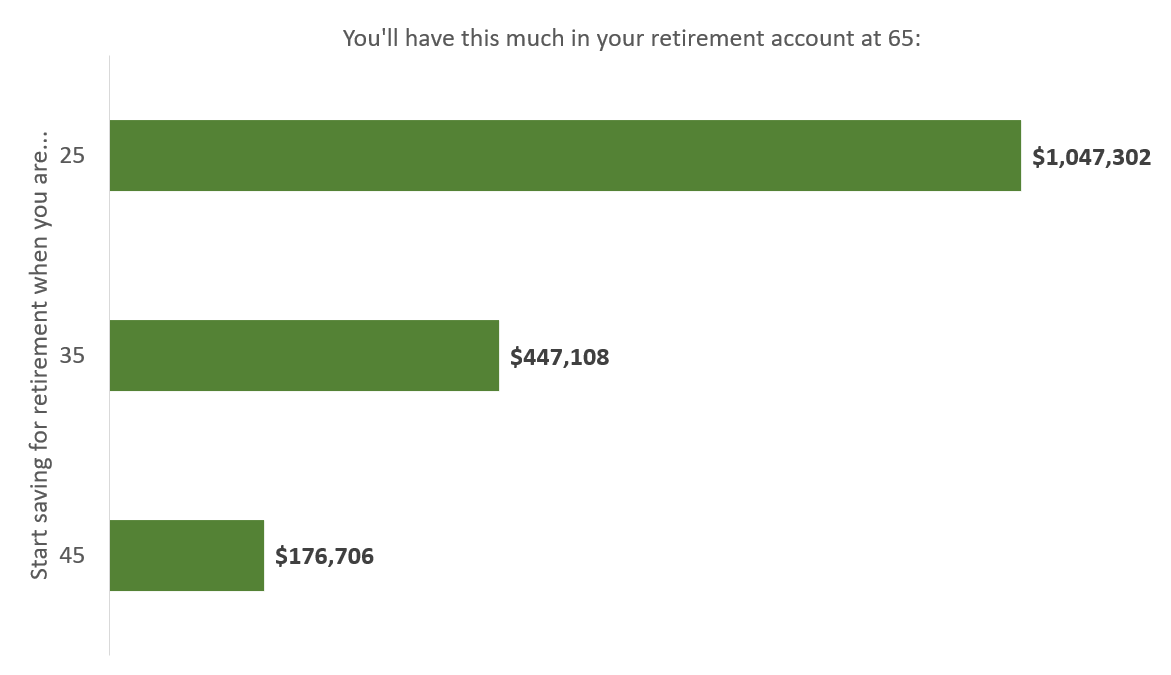
\includegraphics[width=0.8\textwidth]{RetirementGoals}
\end{center}

This graph shows how much you can accumulate if you can save \$300 a month, assuming that you receive an 8\% annual return on your investments, a fairly typical result if, for instance, you invest in index funds, which are mutual funds designed to track the market as a whole over the long term.

That may sound like a lot to save, but this is about the amount that many people spend on a car payment.  What this means is that with relatively small sacrifices, such as driving used cars instead of new ones, you can someday see your retirement account cross the \$1,000,000 threshold.

Let's dig into that chart a bit more.  Notice that if you wait until age 35 to start saving, you won't just save a \emph{bit} less than you would if you started saving earlier; you'll wind up with \emph{less than half}, just by waiting 10 years.  Maybe you can't afford to save \$300 a month right now, but you can afford \$100 a month: start there!

Why is there such a dramatic difference?  It's all due to compound interest, and we learned in the last section that compound interest really flexes its muscles when you give it plenty of time.  Those 10 years between ages 25 and 35 are the most important years in the process, because they are the first years, and the money saved then has the most time to grow.

To show this, let's break down the amount that you will actually deposit in each case, versus the amount you'll earn in interest:
\begin{center}
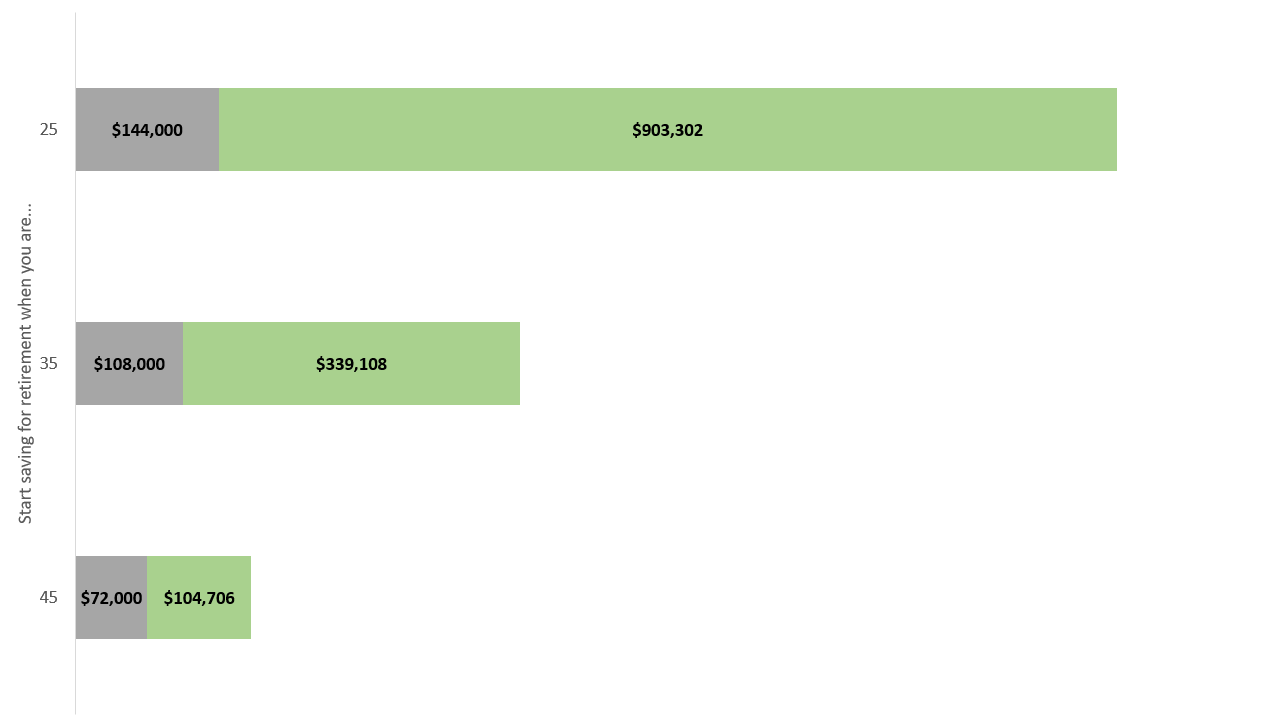
\includegraphics[width=0.8\textwidth]{RetirementGoalsWithInterest}
\end{center}

Notice that if you wait until age 45 to start saving, you'll end up depositing half of what you would if you started at 25, but your final balance will be about \emph{one sixth} of what it could be.  Another way to look at it is that starting at age 25 multiplies your money by over seven times (the ratio of what you actually save and what interest adds), but starting at age 45 only multiplies your money by about two and a half.

In this section, you'll learn how all of those values were calculated, but the conclusion should already be clear: don't wait any longer to start saving!

\subsection{Annuities}
The term \emph{annuity} simply refers to a series of recurring payments.  This is different from what we did in the last section, where we assumed that a single lump-sum deposit was made and a single withdrawal was made later.  We haven't yet dealt with accounts that take regular deposits, but that's what you do for any kind of long-term savings plan: use small, regular payments to grow over time.

In this section, we'll discuss two types of annuities, which are similar, but the formulas are slightly different.

\begin{formula}{Types of Annuity}
\paragraph{Savings Annuity} This is the kind that you use to save for retirement; you make regular deposits over time, and the balance slowly grows because of two factors: your deposits and the accruing interest.

\paragraph{Payout Annuity} When you retire, you stop making payments into your retirement plan, and you start receiving regular payouts instead, which replace your paycheck.  In this case, we start the problem with a lump sum (what you managed to save) and compare that lump sum with the payment amount that you receive.
\end{formula}

If you do more research on annuities, you'll find that there are other variations, such as lifetime annuities, or that annuities apply in other situations (usually some large payment such as life insurance or lottery winnings can be paid out using annuities), but our focus will be on retirement savings, since that's the most common scenario.

For our purposes, the basic process looks something like this: starting today, you can deposit money into a savings annuity, and we can calculate what your final balance will be when you retire.  Then, we can fast-forward to the day of retirement, and projecting how much your account will hold, we can find out how much you can expect to receive as a monthly payment in retirement.  We can also work backward from how much you'll need in retirement to calculate the balance you need when you retire, then work backward again to calculate how much you'll need to start saving.
\vfill
\pagebreak

\subsection{Savings Annuities}

Let's start with a simple example to illustrate how a savings annuity works.

\begin{example}[https://www.youtube.com/watch?v=KOIRAWGh9vM]{Savings Annuity}
Suppose you deposit \$100 into a savings account at the end of each year.  If you earn 5\% interest compounded annually, how much will the account hold at the end of 3 years?  How much interest did the account earn?\\

\marginnote{\bfseries Solution}
At the end of the first year, the account holds the \$100 that you deposit then:
\[F_1 = \$100\]
The second year, this \$100 earns interest, plus you deposit another \$100 at the end of the year:
\[F_2 = \$100(1+0.05) + \$100 = \$205\]
The third year, this \$205 earns interest, plus you deposit another \$100 at the end of the year:
\[F_3 = \$205(1+0.05) + \$100 = \$315.25\]
We could continue this pattern indefinitely, but each year, we only need to use the simple interest formula to see how much the previous year's balance has grown, and then add in that year's deposit.\\

At the end of the three years, the account holds \$315.25, and since we deposited a total of \$300 (\$100 each year for 3 years), the account earned a total of \$15.25 in interest.
\end{example}

In theory, we could do that every time we need to calculate the value of an annuity, but that would get tedious very quickly.  The following formula is derived based on that process (details are at the end of this section, in case you'd like to see the algebra).

\begin{formula}{The Future Value of a Savings Annuity}
If regular deposits of $PMT$ are made $n$ times per year into an annuity paying an interest rate of $r$ compounded $n$ times per year, the future value of the annuity at the end of $t$ years is given by
\[F=\dfrac{PMT\left[\left(1+\dfrac{r}{n}\right)^{nt}-1\right]}{\left(\dfrac{r}{n}\right)}\]
\end{formula}

This formula looks complicated, but with a little practice, you'll be able to use it, for instance, to verify the numbers in the retirement discussion at the beginning of the section.

By the way, we may also start by determining how much we want the account to hold at the end, and use that to calculate $PMT$.  To do that, we need to solve the formula above for $PMT$, which means multiplying both sides by $r/n$ and dividing both sides by the expression in brackets:
\[PMT = \dfrac{F\left(\dfrac{r}{n}\right)}{\left[\left(1+\dfrac{r}{n}\right)^{nt}-1\right]}\]
You can choose to keep this formula handy as well, or you can simply do the algebra each time.  It helps to enter all the values and simplify as much as possible on the right hand side, and then simply divide $F$ by that simplified value.
\pagebreak

\begin{example}[https://www.youtube.com/watch?v=X1oXL3ZjcCU]{Traditional IRA}
A traditional individual retirement account (IRA) is a retirement account in which the money you invest is tax-exempt (you can deduct your contributions on your income tax return) until you withdraw it.  Thus, taxes are deferred until you retire.  If you deposit \$250 each month into an IRA earning 7\% interest, how much will you have in the account after 35 years?

\sol
Organize the given information:
\begin{center}
\begin{tabular}{r l l}
$PMT$ & \$250 & The regular deposit\\
$r$ & 0.07 & 7\% annual rate\\
$n$ & 12 & Deposits are made monthly\\
$t$ & 35 & Deposits are made for 35 years
\end{tabular}
\end{center}

Putting it all together in the formula:
\begin{align*}
F &= \dfrac{\$250\left[\left(1+\dfrac{0.07}{12}\right)^{(12)(35)}-1\right]}{\left(\dfrac{0.07}{12}\right)} = \boxed{\$450,264}
\end{align*}

Notice\marginnote{$(\$250)(12)(35) = \$105,000$} that you deposited \$250 every month, 12 months a year for 35 years, for a total of \$105,000.  That means that the account earned approximately $\$450,264-\$105,000 = \$345,264$ in interest, or to put it another way, the deposits more than quadrupled due to interest.
\end{example}

%\paragraph{Note:} we rounded here to the nearest dollar, since the dollar amount is so large, making the cents less significant.  There's no rule about this, but simply a matter of preference.

\begin{try}[http://izzomath.com/103text/finance/example4.2/story.html]
If you deposit \$800 every year into a traditional IRA earning 4\% interest, how much will the account hold after 25 years?
\end{try}

There is another common type of retirement account: the Roth IRA.  The idea behind a Roth IRA was originally proposed in 1989 by Senator William Roth of Delaware and established by the Taxpayer Relief Act of 1997.

The differences between traditional and Roth IRAs do not affect the calculations in the examples, but you may hear both terms discussed, so we'll include a short comparison here just for your interest (you can skip this if you prefer).

\checkoddpage
\ifoddpage{
\begin{adjustwidth}{-0.25in}{-1.75in}
\begin{proc}{Traditional vs. Roth IRA}
The main difference between the two types of IRA (individual retirement accounts) revolves around taxes.  With a traditional IRA, contributions are tax-free (you can deduct these on your tax return) and you pay taxes when you withdraw the funds in retirement.  Roth IRA contributions, on the other hand, are taxed when you make them, but when you make withdrawals after retiring, you won't pay taxes then.\\

Thus, when comparing the two, the question is: do you expect to pay higher taxes now, or when you are retired?  It's hard to know for sure, because your income may be higher or lower than it is now, and many of the deductions you'll take advantage of in the near term (like mortgage insurance, dependent expenses, or education costs) will not apply when you are retired.\\

There are other qualitative differences, like the fact that a traditional IRA will require you to start withdrawing when you reach 70.5 years of age, but Roth IRAs don't have that restriction, making them a popular vessel for transferring wealth to inheritors.

\paragraph{Contribution Limits (2020)}
The most you can contribute to either kind of IRA (or a combination of the two) in a single year is \$6,000 if you're younger than 50, or \$7,000 if you're 50 or older.

\paragraph{Income Limits (2020)}
Traditional IRAs have no income limits, but you can't contribute to Roth IRAs if you make too much money.  For instance, the current limit for single individuals is \$124,000, and \$196,000 for married couples; if your adjusted income is higher, you can only contribute to a traditional IRA that year.\\

One final note: both kinds of IRA allow first-time homebuyers to withdraw up to \$10,000 to pay for qualified housing costs.
\end{proc}
\end{adjustwidth}
} \else{
\begin{adjustwidth}{-1.75in}{-0.25in}
\begin{proc}
The main difference between the two types of IRA (individual retirement accounts) revolves around taxes.  With a traditional IRA, contributions are tax-free (you can deduct these on your tax return) and you pay taxes when you withdraw the funds in retirement.  Roth IRA contributions, on the other hand, are taxed when you make them, but when you make withdrawals after retiring, you won't pay taxes then.\\

Thus, when comparing the two, the question is: do you expect to pay higher taxes now, or when you are retired?  It's hard to know for sure, because your income may be higher or lower than it is now, and many of the deductions you'll take advantage of in the near term (like mortgage insurance, dependent expenses, or education costs) will not apply when you are retired.\\

There are other qualitative differences, like the fact that a traditional IRA will require you to start withdrawing when you reach 70.5 years of age, but Roth IRAs don't have that restriction, making them a popular vessel for transferring wealth to inheritors.

\paragraph{Contribution Limits (2020)}
The most you can contribute to either kind of IRA (or a combination of the two) in a single year is \$6,000 if you're younger than 50, or \$7,000 if you're 50 or older.

\paragraph{Income Limits (2020)}
Traditional IRAs have no income limits, but you can't contribute to Roth IRAs if you make too much money.  For instance, the current limit for single individuals is \$124,000, and \$196,000 for married couples; if your adjusted income is higher, you can only contribute to a traditional IRA that year.\\

One final note: both kinds of IRA allow first-time homebuyers to withdraw up to \$10,000 to pay for qualified housing costs.
\end{proc}
\end{adjustwidth}} \fi

We've seen an example of calculating $F$ given $PMT$; let's switch things around and look for the payment amount if we know how much we want the account to hold.

\begin{example}[https://www.youtube.com/watch?v=TWZhZoh9TG4]{How Much Should You Save?}
You want to have \$500,000 in your account when you retire in 35 years.  If your retirement account earns 5\% interest, how much should you deposit each month to reach your retirement goal?

\sol
Now everything except for $PMT$ is given, and that is what we are trying to determine.
\begin{center}
\begin{tabular}{r l l}
$F$ & \$500,000 & The future value\\
$r$ & 0.05 & 5\% annual rate\\
$n$ & 12 & Deposits are made monthly\\
$t$ & 35 & Deposits are made for 35 years
\end{tabular}
\end{center}

Putting it all together in the formula:
\begin{align*}
\$500,000 &= \dfrac{PMT\left[\left(1+\dfrac{0.05}{12}\right)^{(12)(35)}-1\right]}{\left(\dfrac{0.05}{12}\right)}\\
\$500,000 &= PMT(1136.092)\\
\boxed{\$440.11} &= PMT
\end{align*}

Having\marginnote{$(\$440)(12)(35) = \$184,846.20$} half a million dollars may sound like an unattainable goal, but by making regular deposits, it becomes possible.  Notice that in this case, you'll deposit a total of \$184,846, which means that the account earns\marginnote{$\$500,000 - \$184,846 = \$315,154$} \$315,154, or close to twice the amount that you deposit.
\end{example}

We could also have used the alternate form of the formula where $PMT$ is isolated, but this example illustrates how to simplify and solve for $PMT$ by using the same formula as before.  It's up to you which process you prefer: a bit more algebra, or keeping track of another formula.

\begin{try}[http://izzomath.com/103text/finance/example4.4/story.html]
You want to have \$800,000 in your account when you retire in 40 years.  If your retirement account earns 6.7\% interest, how much should you deposit each month to reach your retirement goal?
\end{try}

In case the discussion at the beginning of the section wasn't enough, let's look at another example emphasizing the same point with a slightly different scenario.  We'll consider two recent college graduates.  Emma learns her lesson and begins saving immediately, while Jason is overwhelmed by his expenses immediately as he begins to work and he neglects to save.  After 20 years, Jason decides to try to catch up.  Let's see how that works out (spoiler alert: Emma winds up better off).

Suppose Jason and Emma graduate the same year and begin working in adjacent cubicles; they're each 23 years old, and they'll both work for 45 years.  Let's assume that both get a 7\% interest rate in their retirement accounts. 

\begin{example}[https://www.youtube.com/watch?v=9hcZL9uCEoY]{Start Saving Early}
\begin{enumerate}[(1)]
\item If Emma begins saving \$400 every month right away and does so for 45 years, how much will her account hold when she retires?\\

Use the savings annuity formula:
\begin{align*}
F &= \dfrac{\$400\left[\left(1+\dfrac{0.07}{12}\right)^{(12)(45)}-1\right]}{\left(\dfrac{0.07}{12}\right)}\\
&\approx \boxed{\$1,517,038}
\end{align*}

\item If Jason begins saving 20 years later, and he saves \$1000 every month for 25 years, how much will his account hold when he retires?\\

Use the savings annuity formula:
\begin{align*}
F &= \dfrac{\$1000\left[\left(1+\dfrac{0.07}{12}\right)^{(12)(25)}-1\right]}{\left(\dfrac{0.07}{12}\right)}\\
&\approx \boxed{\$810,072}
\end{align*}
Notice that he has to save more than her (\$300,000 versus \$216,000), but he winds up way behind, because his savings didn't have as much time to grow.

\item How much would Jason have to save each month for 25 years to match Emma's final total?\\

To find this out, set $F$ equal to Emma's final total, and solve for $PMT$ using $t=25$:
\begin{align*}
\$1,517,038 &= \dfrac{PMT\left[\left(1+\dfrac{0.07}{12}\right)^{(12)(25)}-1\right]}{\left(\dfrac{0.07}{12}\right)}\\
\boxed{\$1873} &\approx P
\end{align*}
He'd have to save much, much more each month to catch up to Emma, and in total this would mean saving \$561,816 (again, compared to the \$216,000 that Emma saves in total).

\item Compare their contributions to their final balances.
\begin{enumerate}[(a)]
\item Emma contributes a total of $\$400 \times 12 \times 45 = \$216,000$, which means that her account earned \$1,301,038 in interest.
\item Under Jason's first plan, he contributes \$300,000 (more than Emma, even though his final balance is much smaller), so he only earns \$510,072 in interest.
\item With Jason's modified plan where he contributes \$1873 each month, he pays in a total of \$561,816, earning \$955,222 in interest.  This interest is so large, though, because of the large payments he makes, which grow the balance quickly, and not due to the length of time given for growth, which is where compound interest really shines.
\end{enumerate}
\end{enumerate} 
This lesson bears repeating: start saving early!
\end{example}
\vfill
\pagebreak

\subsection{Payout Annuities}
We're ready now to shift from savings annuities, where you make regular deposits to save toward a final lump sum, to payout annuities, in which that lump sum is repaid to you in regular payments and the remaining balance continues to earn interest in the meantime.  Once again, this is typically the shift that occurs upon retirement, and it's important to understand in order to intelligently plan for retirement.

As with savings annuities, we'll start with the formula (the derivation for this one can also be found at the end of the section).

\begin{formula}{Payout Annuities}
If a starting balance of $P$ is paid out in regular payments of $PMT$ from an annuity earning $r$ interest compounded $n$ times per year, and the payments are made $n$ times per year, the following relationship holds:
\[P = \dfrac{PMT\left[1-\left(1+\dfrac{r}{n}\right)^{-nt}\right]}{\left(\dfrac{r}{n}\right)}\]
Notice the negative exponent; be careful when entering that into your calculator.
\end{formula}

Notice that the formula is set up to solve for $P$ rather than $PMT$; this is mostly for convenience, because when planning for retirement, you usually start by deciding how much you need to receive every month to cover your needs.  We can, however, turn the problem around: if we start knowing (or assuming) how much the account will hold at the beginning, we can solve for $PMT$ just as we did with savings annuities.
\[PMT = \dfrac{P\left(\dfrac{r}{n}\right)}{1-\left(1+\dfrac{r}{n}\right)^{-nt}}\]
Again, you could keep track of this formula as well, or simply solve for $PMT$ whenever needed.

\begin{example}[https://www.youtube.com/watch?v=A2pKYPSXUbw]{Payout Annuity}
After retiring, you want to be able to take \$1000 every month from your retirement account for 20 years.  If the account earns 6\% interest, how much will you need in your account when you retire?

\sol
Organize the given information:
\begin{center}
\begin{tabular}{r l l}
$PMT$ & \$1000 & The regular withdrawal\\
$r$ & 0.06 & 6\% annual rate\\
$n$ & 12 & Withdrawals are made monthly\\
$t$ & 20 & Withdrawals are made for 20 years
\end{tabular}
\end{center}

Putting it all together in the formula:
\begin{align*}
P &= \dfrac{\$1000\left[1-\left(1+\dfrac{0.06}{12}\right)^{-(12)(20)}\right]}{\left(\dfrac{0.06}{12}\right)}\\
&\approx \boxed{\$139,581}
\end{align*}

You'll need to have approximately \$139,600 in your account when you retire.  Notice that you'll withdraw \$240,000 (\$1000 for 240 months).  You're able to pull out more than you have at retirement because you don't withdraw it all at once, but take it out little by little as you need it, allowing the remainder to earn interest before you take it out.  This difference represents \$100,400 in interest earned during those 20 years of retirement.
\end{example}

\begin{try}[http://izzomath.com/103text/finance/example4.6/story.html]
After retiring, you want to be able to take \$1500 every month from your retirement account for 15 years.  If the account earns 4.5\% interest, how much will you need in your account when you retire?
\end{try}

\begin{proc}{Calculator Note: Evaluating Negative Exponents}
With these problems, you need to raise numbers to negative powers.  Most calculators have a separate button for negating a number that is different than the subtraction button.  Some calculators label this $\boxed{(-)}$\ , and some label it $\boxed{+/-}$\ .

If your calculator has a multiline display, to calculate $1.005^{-240}$, you'd type something like $1.005 \boxed{\wedge}\ \boxed{(-)}\ 240$.

If you have a scientific calculator that only displays a single number at a time, you will most likely need to hit the $\boxed{(-)}$ key after a number to negate it.  Thus, you'd type $1.005\ \boxed{y^x}\ 240\ \boxed{(-)}\ \boxed{=}\ $.

Try it on your calculator and make sure that you get 0.302096 as your answer.
\end{proc}

Finally, let's turn this around and ask the other question: given a fixed amount in our account, how much can we withdraw in regular payments?

\begin{example}[https://www.youtube.com/watch?v=BsqVTSoWOm8]{Withdrawing from a Payout Annuity}
You expect to have \$500,000 in your IRA when you retire, and you want to be able to take monthly withdrawals for a total of 30 years.  If your account earns 8\% interest, how much will you be able to withdraw each month?

\sol
Organize the given information:
\begin{center}
\begin{tabular}{r l l}
$P$ & \$500,000 & The starting balance\\
$r$ & 0.08 & 8\% annual rate\\
$n$ & 12 & Withdrawals are made monthly\\
$t$ & 30 & Withdrawals are made for 30 years
\end{tabular}
\end{center}

This time we want to find $PMT$:
\begin{align*}
\$500,000 &= \dfrac{PMT\left[1-\left(1+\dfrac{0.08}{12}\right)^{-(12)(30)}\right]}{\left(\dfrac{0.08}{12}\right)}\\
\$500,000\marginnote{Note: if you don't round at this step, your answer should be \$3668.82} &= PMT(136.232)\\
\boxed{\$3670} &\approx PMT
\end{align*}

You can plan to withdraw about \$3670 each month for 30 years.
\end{example}

\begin{try}[http://izzomath.com/103text/finance/example4.7/story.html]
A donor gives \$100,000 to a university, and specifies that it is to be used to give annual scholarships for the next 20 years.  If the university can earn 4\% interest, how much can they give in scholarships each year?
\end{try}
\vfill
\pagebreak

Let's put it all together, and try a full example in which we start with the desired monthly payout during retirement, and determine how to start saving now.  This is the kind of planning that you can do right now for yourself, using the tools we've discussed in this section.

\begin{example}{Planning for Retirement}
Kevin is 30 years old, and he is preparing to begin saving for retirement.  He expects to retire at age 67, and for planning purposes, he assumes he'll live to age 95.  Based on cursory research, he expects that his investments can average a return of 7\% annually, and after retirement, he will move his money into more conservative investments returning 5\% annually.  In order to be able to withdraw \$3000 per month after retirement, how much should he plan to save each month?

\sol
There are two stages to this problem; it's essentially like doing two of the previous examples back-to-back.  First, we need to use the payout annuity formula to find how much Kevin's retirement account must hold at age 67 to meet his goals.  Once we know that, we can work backward using the savings annuity formula to find the payment amount that will lead to that future value.\\

\marginnote{\textbf{1. Find balance at retirement}}
For the first stage, using the payout annuity formula, the following summarizes what we know:
\begin{center}
\begin{tabular}{r l l}
$PMT$ & \$3000 & The regular withdrawal\\
$r$ & 0.05 & 5\% annual rate\\
$n$ & 12 & Withdrawals are made monthly\\
$t$ & 28 & Withdrawals are made for 28 years
\end{tabular}
\end{center}

Putting it all together in the formula:
\begin{align*}
P &= \dfrac{\$3000\left[1-\left(1+\dfrac{0.05}{12}\right)^{-(12)(28)}\right]}{\left(\dfrac{0.05}{12}\right)}\\
&\approx \$541,933
\end{align*}

At age 67, then, Kevin's retirement account needs to hold \$541,933.  Knowing that, we can now shift focus to the savings annuity that he will use between now and age 67 to accumulate that total.\\

\marginnote{\textbf{2. Find savings payment}}
Notice that now the interest rate will change to 7\%, and the amount of time to save will be 37 years (from age 30 to age 67):
\begin{center}
\begin{tabular}{r l l}
$F$ & \$541,933 & The future value\\
$r$ & 0.07 & 7\% annual rate\\
$n$ & 12 & Deposits are made monthly\\
$t$ & 37 & Deposits are made for 37 years
\end{tabular}
\end{center}

Using the savings annuity formula:
\begin{align*}
\$541,933 &= \dfrac{PMT\left[\left(1+\dfrac{0.07}{12}\right)^{(12)(37)}-1\right]}{\left(\dfrac{0.07}{12}\right)}\\
\boxed{\$258.49} &= PMT
\end{align*}

By setting aside a little over \$250 each month into a retirement account, Kevin can build quite a decent nest egg, and ensure that he'll be able to withdraw \$3000 a month after he retires.
\end{example}

\begin{try}
Erika is 27 years old, and plans to retire at age 64.  If she can expect an 8\% return while she's saving, and a 6\% return while she withdraws, how much should she begin saving each month if she expects to live to age 92 and would like to receive \$3500 a month in retirement?
\end{try}

\vfill
\pagebreak

\subsection{Using the TVM Solver}
We can use the TVM solver that was introduced for compound interest in the previous section to solve problems with annuities as well.  Recall the setup of the solver (found under the $\boxed{\textrm{APPS}}$\ menu):
\begin{center}
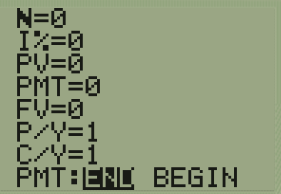
\includegraphics[width=1.8in]{TVMintro}
\end{center}

Notice the entry for PMT (on the fourth line), which we did not use last time.  This is the same as the payment amount $PMT$ in our formulas in this section.

\paragraph{Savings vs. Payout Annuities} The main difference to keep in mind when using the TVM solver is that for a savings annuity, we're using payments to build to a \emph{future value} FV, and with a payout annuity, we have a \emph{present value} PV that gets paid out in regular payments.

So for a problem involving a savings annuity, set PV to 0 and use FV and PMT (find whichever we need to based on knowing the other), and for a payout annuity, set FV to 0 and use PV and PMT.\\

The rest of the information in the menu is the same as before.  In almost every problem, if not every single one, payments occur monthly, so P/Y, and C/Y will both be 12.  Recall that I\% should be entered in percentage form, not decimal form, and you should be all set!\\

We'll show one example for each kind of annuity; both will be repeated from earlier examples for comparison.

\begin{example}{TVM Solver: Future Value for Savings Annuity}
If you deposit \$250 each month into an IRA earning 7\% interest, how much will you have in the account after 35 years?

\sol
Open the TVM solver and enter the information given (remember that N is the total number of payments, so enter \texttt{12*35}.  When you're done, you should have the following:
\begin{center}
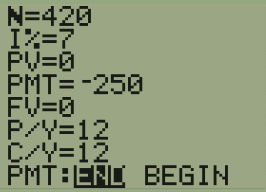
\includegraphics[width=1.8in]{TVMSavingsAnnuityFutureValue}
\end{center}
To solve for the future value, move the cursor over the value for FV, and press $\boxed{\textrm{ALPHA}}$ then $\boxed{\textrm{ENTER}}$ to solve.  You should see the answer entered there:
\begin{center}
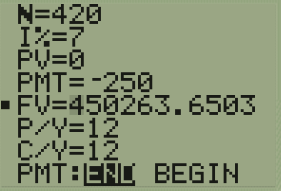
\includegraphics[width=1.8in]{TVMSavingsAnnuityFutureValueSolved}
\end{center}
The final balance will be \$450,264 (verify that this matches what we found using the formula earlier).
\end{example}

\begin{example}{TVM Solver: Payment for Payout Annuity}
You expect to have \$500,000 in your IRA when you retire, and you want to be able to take monthly withdrawals for a total of 30 years.  If your account earns 8\% interest, how much will you be able to withdraw each month?

\sol
Here's the setup (remember, set FV to 0 and work with PV and PMT):
\begin{center}
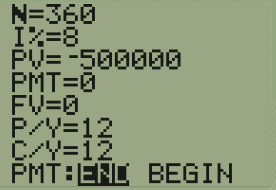
\includegraphics[width=1.8in]{TVMPayoutAnnuityPayment}
\end{center}
Remember that we use negative numbers to indicate money going out from us, and positive for money coming to us (if you forget to do this during setup, it doesn't cause any problems; just mentally reverse the signs).  After solving, you should see this:
\begin{center}
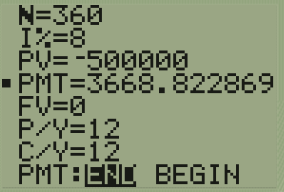
\includegraphics[width=1.8in]{TVMPayoutAnnuityPaymentSolved}
\end{center}
Notice that the answer is slightly different from the one we got using the formula (within a dollar or two), because we rounded partway through that problem.
\end{example}

\begin{try}
Try using the TVM solver to work out the other examples in this section.
\end{try}
\vfill
\pagebreak

\subsection{Using Excel}
Excel has built-in formulas to solve the same problems:
\paragraph{Finding the payment} \texttt{PMT(rate,nper,pv,[fv],[type])}
\paragraph{Finding the future value for a savings annuity} \texttt{FV(rate,nper,pmt,[pv],[type])}
\paragraph{Finding the present value for a payout annuity} \texttt{PV(rate,nper,pmt,[fv],[type])}

In each formula, the items in brackets are optional, and we won't use them here (in case you're curious, the type is the same as the option at the bottom of the TVM solver to switch between beginning-of-month and end-of-month payments).\\

\paragraph{Important note:} the rate used in these formulas is the \textbf{monthly} rate, or the given annual interest rate divide by 12.  Also, nper refers to the number of periods, which is $nt$ in our formulas.

We'll show one example here: calculating the future value of a savings annuity.

\begin{example}{Excel: Future Value for Savings Annuity}
If you deposit \$250 each month into an IRA earning 7\% interest, how much will you have in the account after 35 years?

\sol
Here's the result in Excel:
\begin{center}
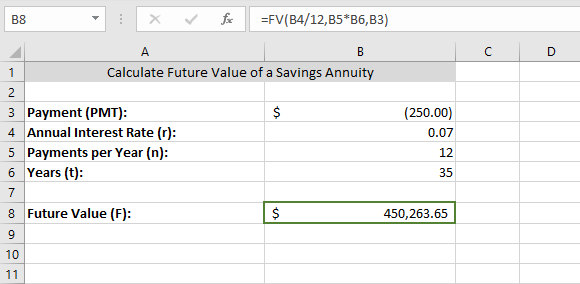
\includegraphics[width=3.5in]{ExcelSavingsAnnuityFutureValue}
\end{center}

Note that the payment amount has parentheses around it; in accounting worksheets, this is how negative values are often indicated.  The convention here is the same as with the TVM solver; since these are payments going out, we count them as negative.\\

\paragraph{Formula:} in cell B8, we entered \texttt{=FV(B4/12,B5*B6,B3)}.  Remember that the rate should be the monthly interest rate, which is why we divided the given annual rate by 12, and the value of nper is equal to the number of payments per year times the number of years.
\end{example}

\begin{try}
Try using Excel to work out the other examples in this section.
\end{try}
\vfill
\pagebreak

\subsection{Deriving the Formulas (optional)}
In case you're \emph{very} curious, and would like to see how the formulas for savings and payout annuities are derived, you can read this.  You can freely skip this part, though, without missing anything major.

\paragraph{Savings Annuity Formula}
Suppose you deposit $P$ dollars (we'll rename this $PMT$ at the end) into a savings annuity each year, and this account earns an interest rate of $r$ compounded annually (we'll handle the case of other compounding periods after we get to the formula).  At the end of the first year, the account contains $P$ dollars:
\[F_1 = P\]
This principal earns interest the second year [growing to $P(1+r)$] so at the end of the second year, the account holds that plus the newly deposited $P$:
\[F_2 = P+P(1+r)\]
Now, in the third year, this balance earns interest again: $(P+P(1+r))(1+r) = P(1+r) + P(1+r)(1+r)$, so the balance at the end of the third year is this plus another $P$:
\[F_3 = P + P(1+r) + P(1+r)^2\]
We can now see the pattern, so we can jump to the arbitrary case; at the end of $t$ years, the account will hold
\begin{equation}
F_t = P + P(1+r) + P(1+r)^2 + P(1+r)^3 + \ldots + P(1+r)^{t-1}
\end{equation}

Now comes the tricky part: we want a simpler formula for $F_t$, so we solve for it in an unexpected way.  First, multiply both sides of the last line by $(1+r)$:
\begin{equation}
F_t + F_tr = P(1+r) + P(1+r)^2 + P(1+r)^3 + \ldots + P(1+r)^{t-1} + P(1+r)^t
\end{equation}
Next, subtract equation (1.1) from equation (1.2), subtracting on both sides of the equation.  Notice that as we do so, almost all of the terms cancel:
\[F_tr = P(1+r)^t-P = P\left[(1+r)^t-1\right]\]
Finally, divide both sides of the equation by $r$ to isolate $F_t$:
\[F_t = \dfrac{P\left[(1+r)^t-1\right]}{r}\]

What if we make deposits monthly rather than yearly?  We'll assume, first of all, that the rate at which we make deposits and the rate at which interest is compounded is the same; in other words, we won't make monthly deposits to an account that compounds weekly, for instance.  If the compounding and the rate of deposit are both represented by $n$, we change this formula in the same way that we changed the compound interest formula to handle different compounding periods:
\begin{itemize}
\item Replace $r$, the annual interest rate, with $\dfrac{r}{n}$, splitting it into compounding periods.
\item Replace $t$ with $nt$ to account for the interest compounding $n$ times per year for $t$ years.
\item Rename $P$ as $PMT$ to emphasize that this is a regular payment.
\end{itemize}
This leads to the general formula:
\[\boxed{F=\dfrac{PMT\left[\left(1+\dfrac{r}{n}\right)^{nt}-1\right]}{\left(\dfrac{r}{n}\right)}}\]

\paragraph{Payout Annuity Formula}
Suppose an account holds $P$ dollars at the beginning, and this will be paid out in regular payments in the amount of $PMT$ dollars each month (or other period, determined by $n$, but this won't affect this derivation).

This account is being drained by these payments, but at the same time, interest is accruing on the remaining balance.  Thus, it turns out the future value that this account would have if it were allowed to grow by compound interest is equal to the future value it has as the reverse of a savings annuity (you can view it as the bank investing in you rather than you investing in the bank).

The future value from compound interest is \[F = P\left(1 + \dfrac{r}{n}\right)^{nt}\]
and the future value as a (reverse) savings annuity is \[F=\dfrac{PMT\left[\left(1+\dfrac{r}{n}\right)^{nt}-1\right]}{\left(\dfrac{r}{n}\right)}\]

Thus, if we set these equal to each other, we get
\[P\left(1 + \dfrac{r}{n}\right)^{nt}=\dfrac{PMT\left[\left(1+\dfrac{r}{n}\right)^{nt}-1\right]}{\left(\dfrac{r}{n}\right)}\]
and all we have to do is solve for $P$, the lump sum amount at the start of the payout process.

To do this, let's rewrite the right-hand side by separating out the denominator:
\[P\left(1 + \dfrac{r}{n}\right)^{nt}=PMT\left(\dfrac{1}{\dfrac{r}{n}}\right)\left[\left(1+\dfrac{r}{n}\right)^{nt}-1\right]\]

Now, if we divide both sides by \[\left(1 + \dfrac{r}{n}\right)^{nt}\] we only need to divide that through the last set of brackets on the right hand side:
\begin{align*}
P &= PMT\left(\dfrac{1}{\dfrac{r}{n}}\right)\dfrac{\left[\left(1+\dfrac{r}{n}\right)^{nt}-1\right]}{\left(1 + \dfrac{r}{n}\right)^{nt}}
\end{align*}

Conveniently, that is the same as the first term in brackets, so that part of the division yields 1, and the rest becomes \[\dfrac{1}{\left(1 + \dfrac{r}{n}\right)^{nt}}.\]
Recall that we can use negative exponents to move terms from the denominator to the numerator, so
\[\dfrac{\left[\left(1+\dfrac{r}{n}\right)^{nt}-1\right]}{\left(1 + \dfrac{r}{n}\right)^{nt}} = \left[1-\left(1 + \dfrac{r}{n}\right)^{-nt}\right]\]

Putting the pieces back together gives the final formula:
\[\boxed{P = \dfrac{PMT\left[1-\left(1+\dfrac{r}{n}\right)^{-nt}\right]}{\left(\dfrac{r}{n}\right)}}\]
\begin{exercises}
\textit{In problems 1--3, a periodic deposit is made into an annuity with the given terms.  Find how much the annuity will hold at the end of the specified amount of time.}\\
\pthree{\begin{center}\begin{tabular}{r l}
Regular deposit & \$250\\
Interest rate & 4\%\\
Frequency & Monthly\\
Time & 15 years\\
Future value & ?
\end{tabular}\end{center}}
\pthree{\begin{center}\begin{tabular}{r l}
Regular deposit & \$10\\
Interest rate & 5\%\\
Frequency & Daily\\
Time & 12 years\\
Future value & ?
\end{tabular}\end{center}}
\pthree{\begin{center}\begin{tabular}{r l}
Regular deposit & \$2000\\
Interest rate & 3\%\\
Frequency & Yearly\\
Time & 22 years\\
Future value & ?
\end{tabular}\end{center}}

\textit{In problems 4--6, find how much should be regularly deposited into an annuity with the given terms in order to have the specified final amount in the account.}\\
\pthree{\begin{center}\begin{tabular}{r l}
Regular deposit & ?\\
Interest rate & 5\%\\
Frequency & Monthly\\
Time & 18 years\\
Future value & \$50,000
\end{tabular}\end{center}}
\pthree{\begin{center}\begin{tabular}{r l}
Regular deposit & ?\\
Interest rate & 6\%\\
Frequency & Weekly\\
Time & 10 years\\
Future value & \$27,000
\end{tabular}\end{center}}
\pthree{\begin{center}\begin{tabular}{r l}
Regular deposit & ?\\
Interest rate & 3.5\%\\
Frequency & Yearly\\
Time & 35 years\\
Future value & \$200,000
\end{tabular}\end{center}}

\textit{In problems 7--9, you want to be able to withdraw the specified amount periodically from a payout annuity with the given terms.  Find how much the account needs to hold to make this possible.}\\
\pthree{\begin{tabular}{r l}
Regular withdrawal & \$1000\\
Interest rate & 5\%\\
Frequency & Monthly\\
Time & 20 years\\
Account balance & ?
\end{tabular}}
\pthree{\begin{tabular}{r l}
Regular withdrawal & \$200\\
Interest rate & 3\%\\
Frequency & Weekly\\
Time & 15 years\\
Account balance & ?
\end{tabular}}
\pthree{\begin{tabular}{r l}
Regular withdrawal & \$20,000\\
Interest rate & 5.5\%\\
Frequency & Yearly\\
Time & 25 years\\
Account balance & ?
\end{tabular}}

\textit{In problems 10--12, you expect to have the given amount in an account with the given terms.  Find how much you can withdraw periodically in order to make the account last the specified amount of time.}

\pthree{\begin{center}\begin{tabular}{r l}
Regular withdrawal & ?\\
Interest rate & 4\%\\
Frequency & Monthly\\
Time & 18 years\\
Account balance & \$300,000
\end{tabular}\end{center}}
\pthree{\begin{center}\begin{tabular}{r l}
Regular withdrawal & ?\\
Interest rate & 5\%\\
Frequency & Weekly\\
Time & 20 years\\
Account balance & \$250,000
\end{tabular}\end{center}}
\pthree{\begin{center}\begin{tabular}{r l}
Regular withdrawal & ?\\
Interest rate & 2.85\%\\
Frequency & Monthly\\
Time & 30 years\\
Account balance & \$1,000,000
\end{tabular}\end{center}}

\ptwo{You deposit \$200 each month into an account earning 3\% interest compounded monthly.
\begin{enumerate}[(a)]
\item How much will you have in the account in 30 years?
\item How much total money will you put into the account?
\item How much total interest will you earn?
\end{enumerate}}
\ptwo{You deposit \$1000 each year into an account earning 8\% interest compounded annually.
\begin{enumerate}[(a)]
\item How much will you have in the account in 10 years?
\item How much total money will you put into the account?
\item How much total interest will you earn?
\end{enumerate}}

\ptwo{Evelyn has \$500,000 saved for retirement in an account earning 6\% interest, compounded monthly.  How much will she be able to withdraw each month if she wants to take withdrawals for 20 years?}
\ptwo{Luke already knows that he will have \$750,000 when he retires.  If he sets up a payout annuity for 30 years in an account paying 7\% interest, how much could the annuity provide each month?}

\ptwo{Michael is planning for retirement, and he estimates that he'll want to be able to withdraw \$2500 each month for 30 years once he retires.  He opens a Roth IRA and finds investments that he expects to return 5\% interest compounded monthly.
\begin{enumerate}[(a)]
\item How much will he need to have in the account when he retires in order to meet his goal?
\item How much will he have to deposit each month for the next 40 years in order to get this balance at retirement?
\item How much interest will his deposits earn?
\end{enumerate}}
\ptwo{Rachel is planning for retirement, and she estimates that she'll want to be able to withdraw \$1800 each month for 25 years once she retires.  She opens a Roth IRA and finds investments that she expects to return 3.75\% interest compounded monthly.
\begin{enumerate}[(a)]
\item How much will she need to have in the account when she retires in order to meet her goal?
\item How much will she have to deposit each month for the next 40 years in order to get this balance at retirement?
\item How much interest will her deposits earn?
\end{enumerate}}

\ptwo{Faith is 27 years old, she plans to retire at age 65, and she expects to live to age 92.  She expects that her investments can earn an average return of 8\% until retirement, and after retirement, she plans to earn 4\%.  If she wants to be able to withdraw \$2500 per month after retirement, how much should she start saving each month?}
\ptwo{Caleb is 30 years old, he plans to retire at age 68, and he expects to live to age 90.  He expects that his investments can earn an average return of 6\% until retirement, and after retirement, he plans to earn 5\%.  If he wants to be able to withdraw \$2000 per month after retirement, how much should he start saving each month?}
\end{exercises}

\section{Mortgages and Credit Cards}
\setcounter{ExampleCounter}{1}
\begin{center}
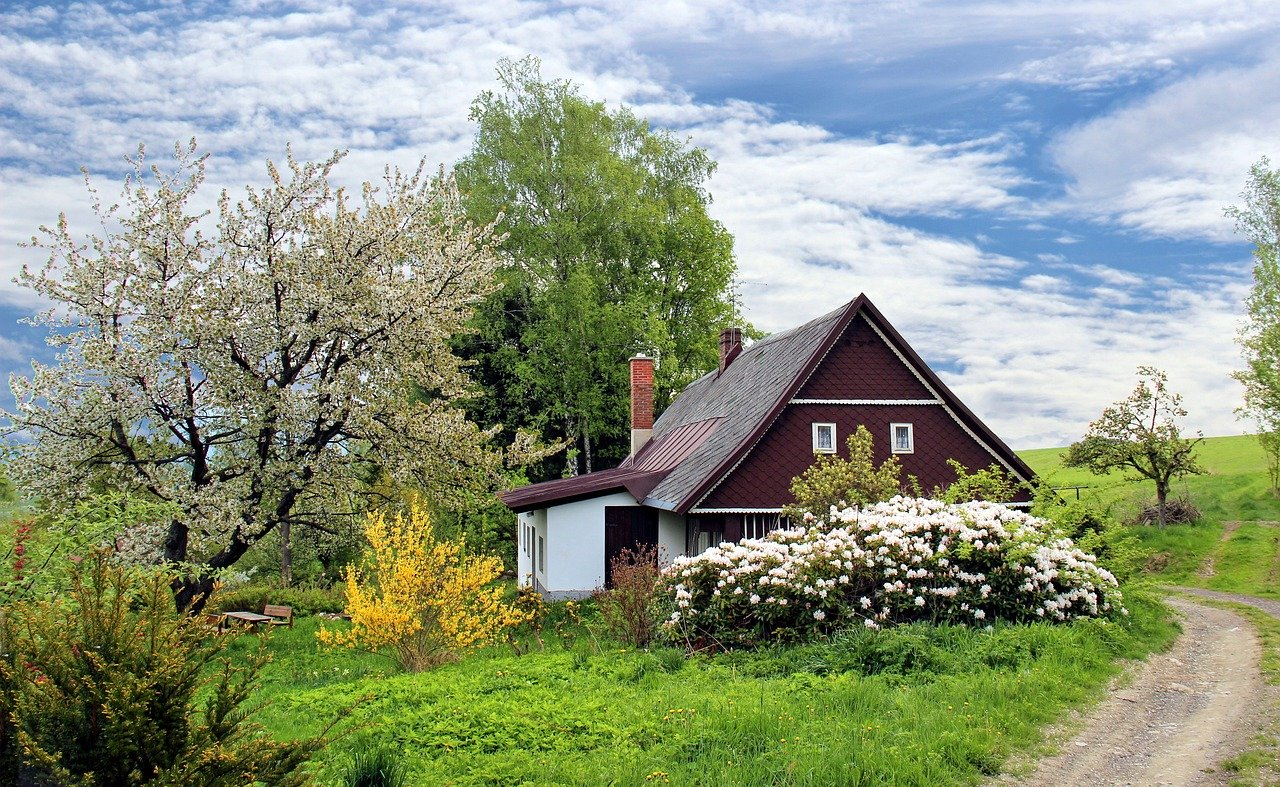
\includegraphics[width=0.8\textwidth]{cottage}
\end{center}

When the time comes to buy a home, you'll need to start shopping around for a \textbf{mortgage}, which is a long-term loan that is secured against whatever home you purchase.  What this means is that if you fail to make your payments and \emph{default} on your loan, the bank can \emph{foreclose} on your house and take it from you in order to pay your debt.  In this section you'll learn how to plan for buying a home.

\subsection{Mortgage Concepts}
Before we start doing calculations with specific formulas, we should discuss some of the terminology related to mortgages.  There are plenty of terms we won't discuss here, but this should be enough to get started.\\

First, a mortgage is an example of an \textbf{installment loan}, which is a loan that is paid off in installments, meaning that you receive a lump sum when you take out the loan, and you pay this loan back in regular monthly payments.  Installment loans are not unique to mortgages; this also describes car payments, for instance, so we'll start with examples about buying a car.\\

Next, you cannot borrow the full amount needed to purchase a home; for a large loan like this, you need to pay a \textbf{down payment} up front.  The reason for this is simple: if none of your own money is tied up in the home, the bank is the one taking all the risk, so you need to come up with part of the money, and from their perspective this investment is your incentive to not default on the loan.  Typical down payments range from 10\% to 20\% of the price of the home.  There are exceptions, like FHA loans, which are guaranteed by the Federal Housing Administration; with these, you can put down as little as 3.5\%.  As we will see, though, it is in your best interest to save up as much as you can for the down payment, especially since a down payment lower than 20\% requires \textbf{mortgage insurance}, which is a fee added to your monthly payment that pays for insurance against the bank's investment.  This insurance will automatically drop off eventually, once you own at least 20\% of the home.\\

The life of a mortgage can vary, but the most typical mortgages are structured for 30 years.  Fifteen-year and 20-year mortgages are also fairly common; the faster you pay back the loan, the less you'll end up paying overall, but the trade-off is that your monthly payments will be higher (we'll see examples of this in this section).  Mortgages can be \textbf{fixed-rate} or \textbf{adjustable-rate}.  As the name implies, the interest rate can change for an adjustable-rate mortgage; the bank will recalculate the rate based on the current market.  You may hear of a mortgage like a 5/1 ARM; this is an adjustable-rate mortgage (ARM) in which the rate is fixed for the first 5 years, and then every year after that, it is recalculated.\\

There are other costs in addition to simply paying back the loan, and we'll account for a few of them in this section.  For instance, when you initiate a mortgage, there are one-time \textbf{closing costs}, which include things like taxes, fees to the lender and title company, land surveys, inspections, and so on.  This just means that when you get ready to buy a home, you need to plan to have your down payment plus the closing costs on hand.
\pagebreak

In addition to the loan payment (often referred to as \emph{principal and interest} or \emph{P\&I}), a few other payments are added each month; the two most common are property taxes and homeowner's insurance.  This is largely for convenience; rather than having to plan for a large insurance or tax payment at the end of the year, those get bundled into your mortgage payment so that you can easily budget for it all each month.  The way this works is that the bank handles making the tax and insurance payments at the end of the year for you.  Throughout the year, as the bank collects your mortgage payment, they set aside the portion of it that corresponds to taxes and insurance and place that into what is called an \textbf{escrow} account.  Then at the end of the year, the bank automatically withdraws the right amount from the escrow account and pays the bills.

\begin{formula}{Summary: Mortgage Terminology}
\paragraph{Installment Loan:} A loan that is paid off in regular (usually monthly) payments.

\paragraph{Down Payment:} A portion of the cost of a home (or car, etc.) that is paid up front; the loan covers the rest of the cost.

\paragraph{Mortgage Insurance:} If a homebuyer puts down less than 20\% of the cost, they must purchase insurance against defaulting.

\paragraph{Closing Costs:} One-time fees that are paid at the time of purchase; these do not go toward the cost of the home.

\paragraph{Escrow:} An account used to hold the portion of the mortgage payment designated for taxes and insurance.
\end{formula}

That's a lot of information all at once, but it's important to understand these terms, because we will use them in the examples in this section.

\subsection{Installment Loan Formula}
At the core of the problems we'll be doing a bit later is the calculation of the loan payment, which is sometimes called P\&I.  This means that this payment is used to slowly pay down the principal of the loan, but it also must pay for the interest that the loan is accruing even as it is being paid off.

This may sound complicated now, but toward the end of the section, we'll break down exactly how a payment is divided between principal and interest, using \emph{amortization tables}.

\paragraph{Calculating the payment on an installment loan:} It turns out that we've actually seen this formula before: it's the one for finding the payment amount for a payout annuity.\\

To see this, imagine that you had \$5000 invested at a bank and you started taking out payments while earning interest (a payout annuity), and after 5 years your balance was zero.  Now flip that around and put yourself in the position of a bank: now the lender is investing \$5000 in you (you take a loan of \$5000) and you start to pay them back in equal payments as the remaining balance earns interest, and after 5 years the balance is zero.\\

Since we're generally interested in finding the payment amount (we usually start by knowing how much we need to borrow), we'll use the version of the payout annuity formula that is solved for $PMT$, but if you want to start with what monthly payment you can afford and find out how much you can borrow, you can rearrange this formula, or simply refer to the version that we mainly used with payout annuities.\\

\begin{formula}{Installment Loan Payment}
If an installment loan of $P$ is taken out at an interest rate of $r$ compounded $n$ times a year, and paid back in equal payments $n$ times a year over $t$ years, the payment amount $PMT$ is given by
\[PMT = \dfrac{P\left(\dfrac{r}{n}\right)}{1-\left(1+\dfrac{r}{n}\right)^{-nt}}\]
\end{formula}

Let's do a few examples, starting with car loans, since that way we don't have to worry about escrow accounts and closing costs just yet.

\begin{example}[https://www.youtube.com/watch?v=RVUWTbil3fQ]{Car Loan}
If you take out an auto loan of \$11,000 at 4\% interest for 60 months, what will your monthly payment be?\\

\sol
Notice that we haven't mentioned a down payment here, but you are probably (hopefully) not borrowing the full cost of the car.  Many car dealers will offer 0\% down loans, but it is in your best interest to only borrow what you have to, not as much as they will offer you.

Start by organizing the given information:
\begin{center}
\begin{tabular}{r l l}
$P$ & \$11,000 & The loan amount\\
$r$ & 0.04 & 4\% interest rate\\
$n$ & 12 & Payments made monthly\\
$t$ & 5 & 60 months = 5 years
\end{tabular}
\end{center}

Simply use the formula:
\begin{align*}
PMT &= \dfrac{\$11,000\left(\dfrac{0.04}{12}\right)}{1-\left(1+\dfrac{0.04}{12}\right)^{-(12)(5)}}\\
&= \boxed{\$202.58}
\end{align*}
Thus you'll end up paying \$202.58 every month for five years.
\end{example}

\begin{try}[http://izzomath.com/103text/finance/example5.1/story.html]
If you take out an auto loan of \$15,000 at 5.6\% interest for 72 months, what will your monthly payment be?
\end{try}

Now let's flip the question around: if you can budget for a car payment, how much of a loan can you afford?

\paragraph{Note:} there's a common pitfall here.  Depending on what salesperson you talk to, they may attempt to start with this question.  The reason is that it's easy for you to imagine spending \$50 more each month, but if they told you how much of a total difference that makes up front, the number would be much more intimidating.  You should always run your own calculations to check things like how much the total cost will change, and how much the total interest charge would change over time.
\pagebreak

\begin{example}[https://www.youtube.com/watch?v=ydmN5lt5g20]{How Much Can You Afford?}
You can afford a monthly car payment of \$250.  If you find a bank offering 4.85\% interest on a 60 month loan, what is the largest car loan you can afford?\\

\sol
In this case $PMT$ is known and $P$ is the unknown that we want to find:
\begin{center}
\begin{tabular}{r l l}
$PMT$ & \$250 & The loan amount\\
$r$ & 0.0485 & 4.85\% interest rate\\
$n$ & 12 & Payments made monthly\\
$t$ & 5 & 60 months = 5 years
\end{tabular}
\end{center}

Now use the formula and solve for $P$:
\begin{align*}
\$250 &= \dfrac{P\left(\dfrac{0.0485}{12}\right)}{1-\left(1+\dfrac{0.0485}{12}\right)^{-(12)(5)}}\\
\$250 &= P(0.0188)\\
\boxed{\$13,296} &\approx P
\end{align*}
You can afford a car loan of \$13,296 under these terms; of course, this is the maximum you can afford, so it wouldn't hurt to take out a smaller loan that this if you can.
\end{example}

\begin{try}[http://izzomath.com/103text/finance/example5.2/story.html]
You can afford a monthly car payment of \$300.  If you find a bank offering 6.7\% interest on a 48 month loan, what is the largest car loan you can afford?
\end{try}

\begin{example}[https://www.youtube.com/watch?v=rhTeMJm8-Lc]{Actual Cost}
You see a TV ad that says ``We can put you in the car of your dreams!!! Drive this brand-new \$25,000 car off the lot with only \$500 down and a monthly payment of \$550 for 60 months.''  How much do you end up actually paying for the car?\\

\solline
\marginnote{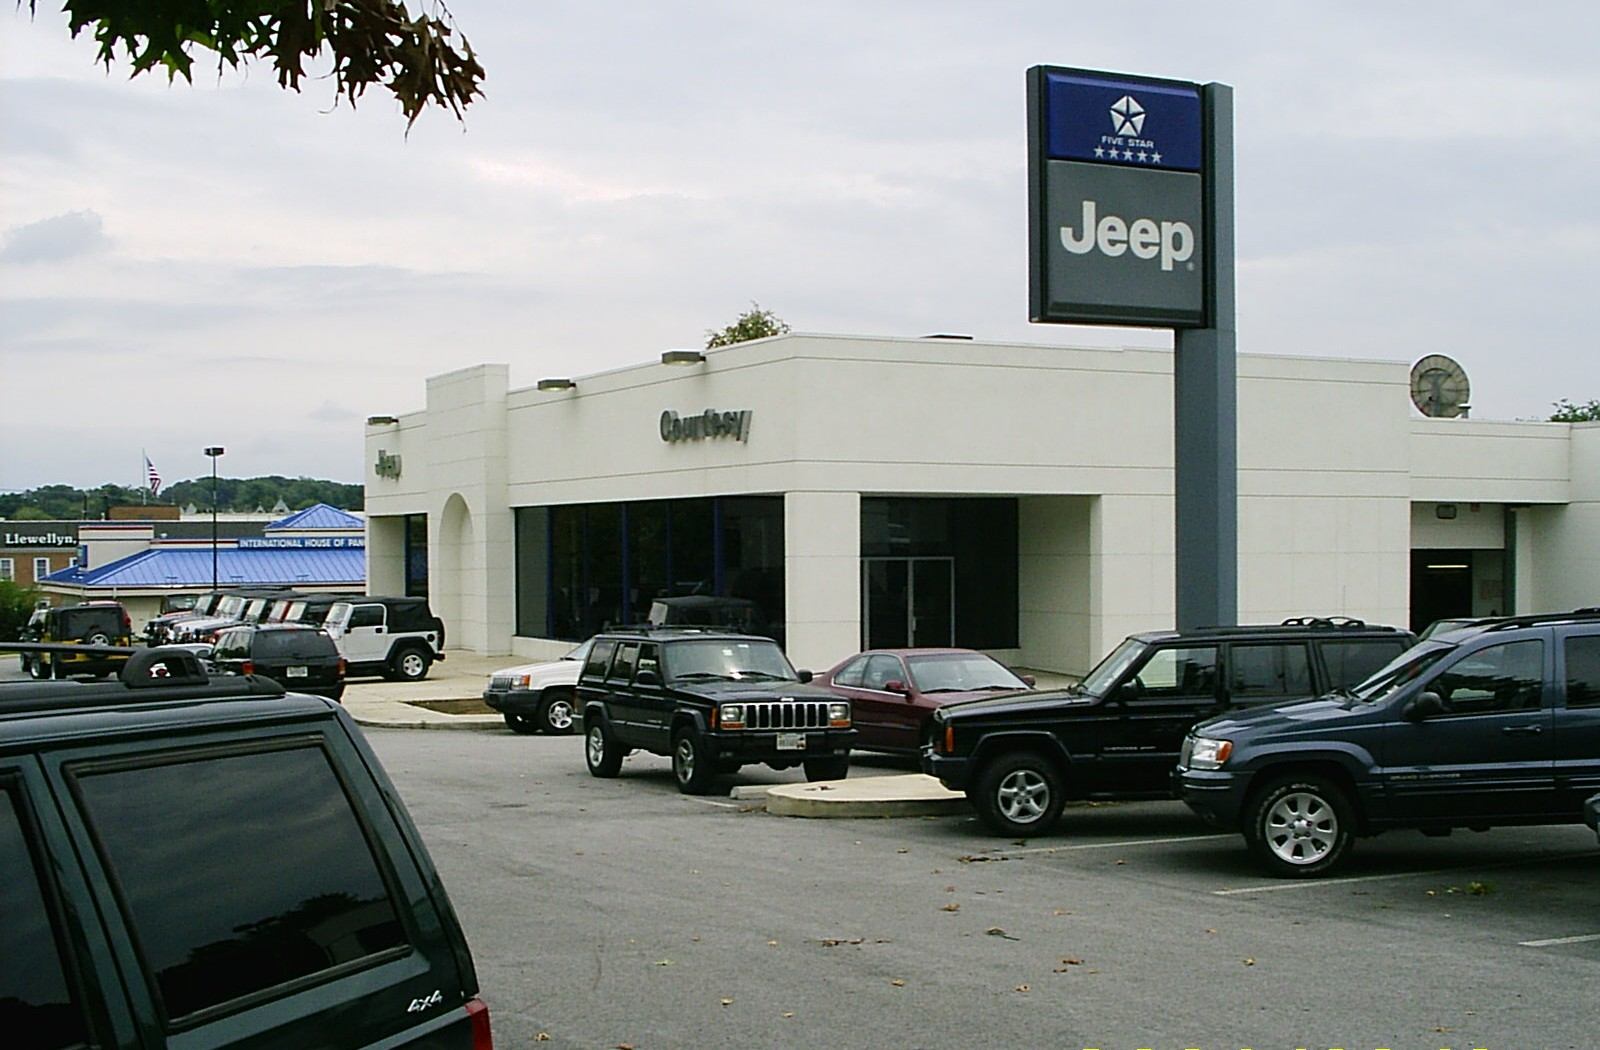
\includegraphics[scale=0.06]{CarDealer1}}
First, let's find out how much the car actually costs you.

The down payment is the amount that is due at the beginning, so if we add that to 60 payments of \$550, we'll have the total amount that comes out of your pocket:
\[\$500 + (60)(\$550) = \$33,500\]

This means that you pay \$33,500 for a \$25,000 car, and the difference is the interest on the loan:\marginnote{\footnotesize\textcolor{black!60}{Photo by Christopher Ziemnowicz}}
\[\$33,500 - \$25,000 = \boxed{\$8500}\]

Are you really willing to pay \$8500 in interest to have the car now, or can you save up first and pay for it in cash---at least in part---to reduce this interest cost?
\end{example}

\begin{try}[http://izzomath.com/103text/finance/example5.3/story.html]
A boat costs \$12,000, and you're offered a loan that requires \$1000 down and \$250 a month for 60 months.  Find the total amount you would pay for the boat and the amount of interest you would pay with this loan.
\end{try}

This example emphasizes an important point: when you're offered a loan, don't focus on the monthly payment; instead, calculate the total cost of the loan and decide if it is worth it to you.
\vfill
\pagebreak

\subsection{Mortgage Example}
If you need to, you can review the terminology introduced at the beginning of the section, because we'll be using those terms in the following examples.

\paragraph{Fair warning:} The next example is a long one, because it includes all the components we discussed at the beginning of the section.  The good news is that this is a pretty realistic example, so if you can understand this, you'll be well prepared for the real thing.

\begin{example}{Buying a Condo}
\marginnote{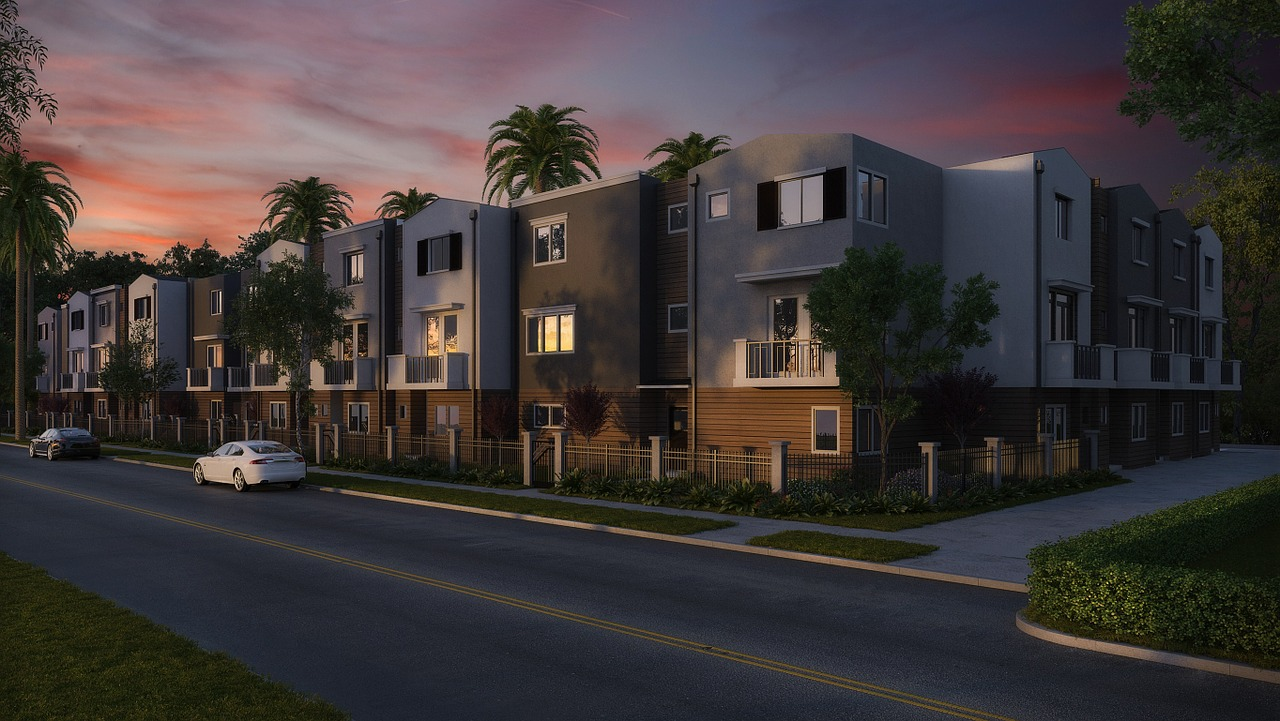
\includegraphics[width=1.5in]{Condo1}}
The price of a condominium is \$180,000, and your bank offers a 30-year fixed mortgage at 4\% interest.  You have \$32,000 available right now.
\begin{enumerate}[(a)]
\item Your banker tells you to expect \$5000 in closing costs.  What percentage down payment can you afford?  Will you need mortgage insurance?
\item What will the principal be on the mortgage?
\item What will your monthly P\&I payment be?
\item In addition to principal and interest, your monthly payment will need to account for property taxes, homeowners insurance, and mortgage insurance, if necessary (find out in part (a)):
\begin{center}
\begin{tabular}{l r}
\textbf{Property Taxes:} & 1.5\% of the home value per year\\
\textbf{Homeowners Insurance:} & \$900 per year\\
\textbf{Mortgage Insurance:} & \$40 per month
\end{tabular}
\end{center}
What will your total monthly payment amount be?
\item How much will you pay in total over 30 years in principal and interest?
\item How much interest will you pay in total?
\end{enumerate}

\sol
There's a lot here, but if we take it one part at a time, the actual calculations are fairly simple.

\begin{enumerate}[(a)]
\item Down payment and mortgage insurance:

Since you need to set aside \$5000 for closing costs, this leaves \[\$32,000 - \$5000 = \$27,000\] for a down payment.  To find what percentage this represents of \$180,000, divide the down payment by the total cost:
\[\dfrac{\$27,000}{\$180,000} = 0.15 = 15\%\]

Therefore, you can afford a down payment of $\boxed{15\%}$, so \textbf{yes, you must pay for mortgage insurance}.

\item Mortgage principal:

The principal on the mortgage is the amount you need to borrow, or the difference between the cost of the home and the down payment, the portion that you can pay in cash.  Since the down payment will be \$27,000,
\begin{align*}
\textrm{Principal } &= \$180,000 - \$27,000\\
&= \boxed{\$153,000}
\end{align*}

\item Monthly principal and interest payment ($PMT$):

This is where we actually have to pull out a complicated formula:
\[PMT = \dfrac{P\left(\dfrac{r}{n}\right)}{1-\left(1+\dfrac{r}{n}\right)^{-nt}}\]

We know that $P$, the principal, will be \$153,000, the interest rate is 4\% (0.04), and $t$ is 30 years, so we can calculate $PMT$:
\begin{align*}
PMT &= \dfrac{\$153,000\left(\dfrac{0.04}{12}\right)}{1-\left(1+\dfrac{0.04}{12}\right)^{-(12)(30)}}\\
&= \boxed{\$730.45}
\end{align*}

This is the amount we'll pay each month just on the loan, but the next part will add to it to give our total payment amount, including the escrow and mortgage insurance (remember, we \textbf{do} require mortgage insurance in this example, but that will not be true in examples where the down payment is at least 20\%).

\item Total monthly payment:

Starting with the P\&I amount of \$730.45, we also need to add taxes, homeowners insurance, and mortgage insurance.  Start by calculating the monthly cost of each component (divide the yearly cost by 12):
{\small
\begin{center}
\begin{tabular}{l r r}
\textbf{P\&I:} & & \$730.45 per month\\
\textbf{Property Taxes:} & Yearly: $(1.5\%)(\$180,000) = \$2700$ & \$225 per month\\
\textbf{Home Insurance:} & \$900 per year & \$75 per month\\
\textbf{Mortgage Insurance:} & & \$40 per month
\end{tabular}
\end{center}}

Adding them all together:
\begin{align*}
\textrm{Monthly Payment } &= \textrm{ P\&I } + \textrm{ Property Tax }\\
&+ \textrm{ Home Insurance } + \textrm{ Mortgage Insurance }\\
&= \$730.45 + \$225 + \$75 + \$40\\
&= \boxed{\$1070.45}
\end{align*}

The final amount you can expect to pay each month is \$1070.45.

\item Total principal and interest paid:

It's easy to calculate how much you will pay in total for the loan: simply multiply your monthly P\&I payment by the number of payments you will make (12 payments a year for 30 years is $(12)(30) = 360$ payments).  Note that the tax and insurance payments are not involved here; we're simply looking for the total principal and interest paid:
\[(\$730.45)(360) = \boxed{\$262,962}\]

Over 30 years, you'll pay a total of \$262,962 for this condo, including the loan interest.

\item Total interest paid:

Now that we know how much you'll pay in principal \emph{and} interest (from the last part), and we know what the principal on the loan is (part (b)), we can subtract to isolate the interest:

\[\$262,962 - \$153,000 = \boxed{\$109,962}\]

Notice that we didn't subtract the total cost of the condo, only the amount that we had to borrow from the bank (we don't pay interest on the amount covered by the down payment).
\end{enumerate}
\end{example}

\begin{try}
The price of a home is \$340,000, and your bank offers a 30-year mortgage at 3.5\% interest.  You have \$60,000 available right now, and the banker tells you to expect \$8000 in closing costs.  Complete parts (a) - (f) of the previous example, using the same values for taxes and insurance.
\end{try}
\pagebreak

\subsection{Changing the Loan Terms}
Let's take a look now at what happens if we change the terms of the loan.  To begin, we'll set up a baseline using a 30-year fixed-rate loan at 4\% and assume that we're borrowing \$200,000.  We won't need to account for a down payment, closing costs, or escrow, since we're only focused on the loan itself for the time being.

Then we'll see what happens if 
\begin{enumerate}[(a)]
\item the interest rate changes,
\item the loan amount changes (if, for instance, we made a larger down payment),
\item or the length of the loan changes.
\end{enumerate}

To make these comparisons, we'll use the same measurement each time: the total interest paid over the life of the loan.  This is a good number to track, because it gives a sense of how much the loan costs (the principal must be paid back no matter what, but by altering the terms, we can alter the amount of interest).\\

We won't show the details of the calculations here, in order to focus on the results.  If you like, you can refer to the description of using the TVM solver with payout annuities to follow along with the calculations quickly.

\begin{example}{Changing the Interest Rate}
Compare a 30-year fixed-rate loan at 4\% for \$200,000 to the same loan at 3.5\% by finding the total amount paid in interest for both versions.

\sol
To compare the total interest paid in each case, we need to find the monthly payment for each, then multiply this by the number of payments (360 for a 30-year loan) and subtract the principal of the loan (\$200,000):
\begin{center}
\begin{tabular}{r c c}
& \textbf{4\%} & \textbf{3.5\%}\\
\textbf{Monthly payment:} & \$954.83 & \$898.09\\
\textbf{Total paid:} & \$343,738.80 & \$323,312.40\\
\textbf{Interest paid:} & $\boxed{\$143,738.80}$ & $\boxed{\$123,312.40}$
\end{tabular}
\end{center}

By reducing the interest rate by just half of one percentage point, you could save over \$20,000 over time (not to mention that if you invested the \$56.74 that you save each month at 7\%, you could save up nearly \$70,000 over the same time).
\end{example}

\begin{example}{Changing the Loan Amount}
Compare a 30-year fixed-rate loan at 4\% for \$200,000 to the same loan for \$180,000 by finding the total amount paid in interest for both versions.

\sol
We can copy the values from the previous example for the baseline loan, so we only need to calculate the monthly payment and other values for the reduced loan:
\begin{center}
\begin{tabular}{r c c}
& \textbf{\$200,000} & \textbf{\$180,000}\\
\textbf{Monthly payment:} & \$954.83 & \$859.35\\
\textbf{Total paid:} & \$343,738.80 & \$309,366.00\\
\textbf{Interest paid:} & $\boxed{\$143,738.80}$ & $\boxed{\$129,366.00}$
\end{tabular}
\end{center}

In this case, you could save over \$34,000 in total by paying \$20,000 more up front or finding a less-expensive home (or some combination of the two).  Of that, about \$14,000 is the amount saved on interest alone.
\end{example}
\pagebreak

\begin{example}{Changing the Length of the Loan}
Compare a 30-year fixed-rate loan at 4\% for \$200,000 to the same loan for 20 years and for 15 years by finding the total amount paid in interest for all three versions.

\sol
Again, the baseline loan will have the same values as always, and we will only change the length of the loan in the other two cases (note that to calculate the total paid, we multiply the 20-year monthly payment by 240, and we multiply by 180 for the 15-year loan):
\begin{center}
\begin{tabular}{r c c c}
& \textbf{30 years} & \textbf{20 years} & \textbf{15 years}\\
\textbf{Monthly payment:} & \$954.83 & \$1211.96 & \$1479.38\\
\textbf{Total paid:} & \$343,738.80 & \$290,870.40 & \$266,288.40\\
\textbf{Interest paid:} & $\boxed{\$143,738.80}$ & $\boxed{\$90,870.40}$ & $\boxed{\$66,288.40}$
\end{tabular}
\end{center}

Notice the trade-off here: shorter loans require higher monthly payments, because you have to pay down the loan faster, but the end result is that you pay much less in interest overall (a total of over \$77,000 in the most extreme case).  Of course, this all depends on the budget that you can work with.
\end{example}

You could, of course, experiment with changing all three factors at once, but at least these examples give us a sense of the total cost of a loan can change dramatically by adjusting the terms of the loan.  When you start shopping for a mortgage, these are all factors to keep in mind.

\subsection{Amortization Tables}
When you take out a mortgage, you'll receive in your loan packet a long table with hundreds of rows, and it's easy for your eyes to glaze over as you scan the columns of numbers marching down, but we're going to see that an \textbf{amortization table} is actually quite simple to understand.

The concept is this: we've used the term P\&I (principal and interest) to describe the payment you make to the bank to pay back the loan.  Each month, the balance that you currently own accrues interest, and part of your payment goes to pay off that interest.  Whatever is left over after paying interest is used to pay down the balance.

This means that as time goes on, and the balance slowly drops, the amount you owe in interest each month decreases as well, so more of your monthly payment can be used to pay down the balance, driving it down even faster, and the process accelerates.

In practice, you'll notice that at the beginning of the process, a lot of your payment goes toward interest, but later in the life of the loan, the balance will shift, and the majority of your payment will go toward principal.  The formula used to calculate your monthly payment ensures that at the end of the process, the balance drops to 0 exactly.

Here's a visual of what it looks like:
\begin{center}
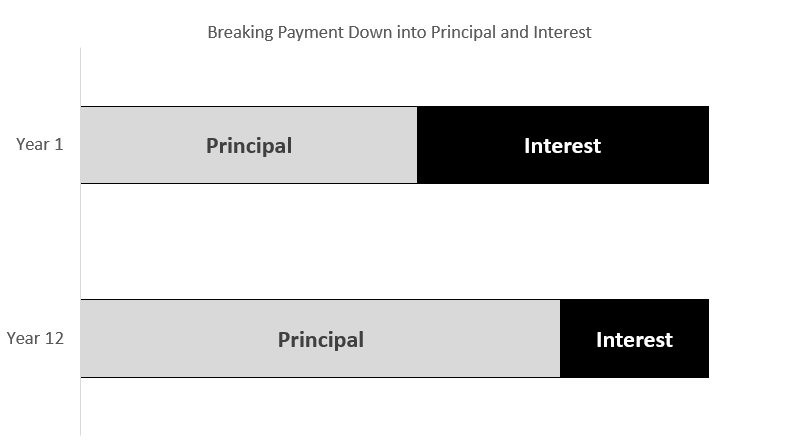
\includegraphics[width=0.8\textwidth]{AmortizationBreakdown}
\end{center}
In year 1, the payment is about evenly split between principal and interest, but by year 12, the overwhelming majority goes to principal (this example was taken from a 20-year mortgage).

Notice that the overall payment never changes; it's just that the line separating the principal from the interest shifts slowly to the right over time.  The final payment of the loan will pay just pennies in interest.

\begin{formula}{Amortization Table}
An \textbf{amortization table} lists the payments of an installment loan in order, showing the amount of each payment that goes toward interest and the amount that goes to toward principal.\\

An amortization table will typically have four columns: the payment number, the interest for that payment, the amount of that payment that goes toward principal, and the remaining balance after the payment.

\begin{center}
\begin{tabular}{|c | c | c | c|}
\hline
Payment Number & Interest Payment & Principal Payment & Loan Balance\\
\hline
& & &
\end{tabular}
\end{center}
\end{formula}

The calculations needed to build an amortization table are very simple, but repetitive, so we'll only build a few rows by hand, and we'll use Excel if we want a full table.

After building a table, you should notice that as you scan down the table, the interest payments decrease, the principal payments increase, and the balance slowly drops.\\

Let's see an example of building a table like this.

\begin{example}[https://www.youtube.com/watch?v=bgFXXvgNB0g]{Loan Amortization Schedule}
Suppose you take out a 20-year mortgage for \$200,000 at 7\% interest, with monthly payments of \$1550.60 (we know how to calculate this now, but it is given to us to simplify this example).  Prepare an amortization schedule for this loan.

\sol
Only one calculation is really needed at each stage---calculating the interest due for that month (everything else follows from that).  To calculate the interest due for a particular month, use the simple interest formula ($I=Prt$); since we're only looking at one payment period, there's no compounding happening.  The principal $P$ will be the loan balance at that point, $r$ is the same for every payment, and $t$ will be 1/12, since we're dealing with a month, a twelfth of a year.
\begin{enumerate}
\item The first payment:
\begin{align*}
\textrm{Interest } &= Prt = (\$200,000)(0.07)\left(\dfrac{1}{12}\right) = \$1166.67\\
\textrm{Principal Payment } &= \textrm{ Monthly Payment } - \textrm{ Interest}\\
&= \$1550.60 - \$1166.67 = \$383.93\\
\textrm{Balance } &= \textrm{ Previous Balance } - \textrm{ Principal Payment}\\
&= \$200,000 - \$383.93 = \$199,616.07
\end{align*}

\item The second payment: the starting balance for the second month is the final balance at the end of the first month, \$199,616.07.
\begin{align*}
\textrm{Interest } &= Prt = (\$199,616.07)(0.07)\left(\dfrac{1}{12}\right) = \$1164.43\\
\textrm{Principal Payment } &=  \$1550.60 - \$1164.43 = \$386.17\\
\textrm{Balance } &= \$199,616.07 - \$386.17 = \$199,229.90
\end{align*}
\end{enumerate}
To fill out the rest of the table, we could continue these calculations until we've covered all 240 payments, but of course this is far too tedious to do by hand, so we have a computer do it for us.  The table below shows a few of the payments, skipping through to show payments at various stages of the loan.
\begin{center}
\begin{tabular}{|>{\centering\arraybackslash\hspace{0pt}}p{1in} | >{\centering\arraybackslash\hspace{0pt}}p{1in} | >{\centering\arraybackslash\hspace{0pt}}p{1.1in} | >{\centering\arraybackslash\hspace{0pt}}p{1in}|}
\hline
{\small Payment Number} & {\small Interest Payment} & {\small Principal Payment} & {\small Balance of Loan}\\
\hline
1 & 1166.67 & 383.93 & 199616.07\\
\hline
2 & 1164.43 & 386.17 & 199229.90\\
\hline
3 & 1162.17 & 388.42 & 198841.47\\
\hline
4 & 1159.91 & 390.69 & 198450.79\\
\hline
\vdots & \vdots & \vdots & \vdots\\
\hline
30 & 1096.12 & 454.47 & 187452.64\\
\hline
31 & 1093.47 & 457.12 & 186995.52\\
\hline
\vdots & \vdots & \vdots & \vdots\\
\hline
145 & 663.44 & 887.16 & 112845.43\\
\hline
146 & 658.26 & 892.33 & 111953.09\\
\hline
\vdots & \vdots & \vdots & \vdots\\
\hline
239 & 17.93 & 1532.66 & 1541.61\\
\hline
240 & 8.99 & 1541.61 & 0.00\\
\hline
\end{tabular}
\end{center}

This illustrates the key features of an amortization table:
\begin{itemize}
\item The interest payment and principal payment in each row add up to the same monthly payment.
\item The balance of the loan slowly shrinks and goes exactly to zero with the last payment.
\item The amount of the payment that goes to interest shrinks each month and the amount that goes to paying down the principal grows by an equal amount.
\end{itemize}
\end{example}

\begin{try}[http://izzomath.com/103text/finance/example5.6/story.html]
If you take out a loan for \$175,000 at 4.5\% interest for 30 years, with a monthly payment of \$886.70, find values for A-F that will correctly fill out the first two rows of the amortization table below.
\begin{center}
\begin{tabular}{|>{\centering\arraybackslash\hspace{0pt}}p{1in} | >{\centering\arraybackslash\hspace{0pt}}p{1in} | >{\centering\arraybackslash\hspace{0pt}}p{1in} | >{\centering\arraybackslash\hspace{0pt}}p{1in}|}
\hline
{\small Payment Number} & {\small Interest Payment} & {\small Principal Payment} & {\small Balance of Loan}\\
\hline
1 & A & B & C\\
\hline
2 & D & E & F\\
\hline
& & &
\end{tabular}
\end{center}
\end{try}
\vfill
\pagebreak

\subsection{Using Excel to Create Amortization Tables}
Again, we would never build a full amortization table by hand, but we can use a spreadsheet program to simplify the process.  To begin, open Excel and enter the details of a loan, as shown.  If we use these values to calculate the rest of the table, we can change any of the terms of the loan and watch the table update immediately for easy comparison.
\begin{center}
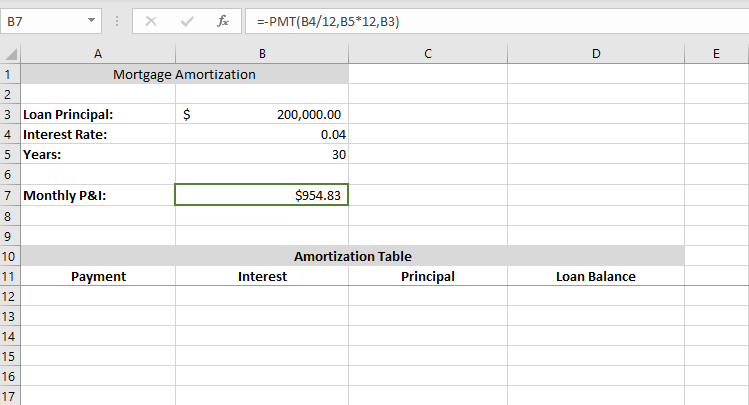
\includegraphics[width=0.75\textwidth]{ExcelAmortizationSetup}
\end{center}

Notice that to calculate the monthly payment, we're using the formula for PMT, as shown in the section on Saving for Retirement.

The key to avoid lots of typing is that you can select a cell or group of cells and drag downward from there, and Excel will try to interpret the pattern that you're trying to express.  For instance, if we place a 1 in cell A12 (the first payment number), and a 2 below it, and we select those two and drag downward, the program will recognize that we want the payment number to grow by one each time, and it will fill in the progression (to drag down and repeat a pattern, move the cursor to the lower right corner of the selection, then click and drag):
\begin{center}
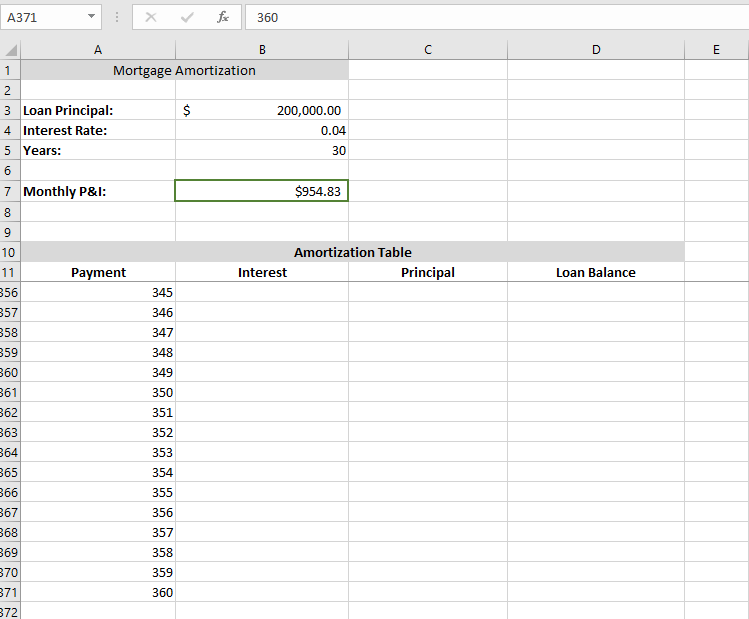
\includegraphics[width=0.75\textwidth]{ExcelAmortizationPaymentNumbers}
\end{center}

We'll carefully fill in the first two rows of the table, then use this functionality to drag the formulas down and generate the rest.
\vfill
\pagebreak

The interest for each month will be calculated by multiplying the balance at the end of the previous month by the interest rate divided by 12.  For the first row, we'll reference the starting balance (\$200,000) but after that, we want this calculation to reference the entry in column D and the previous row.
\begin{center}
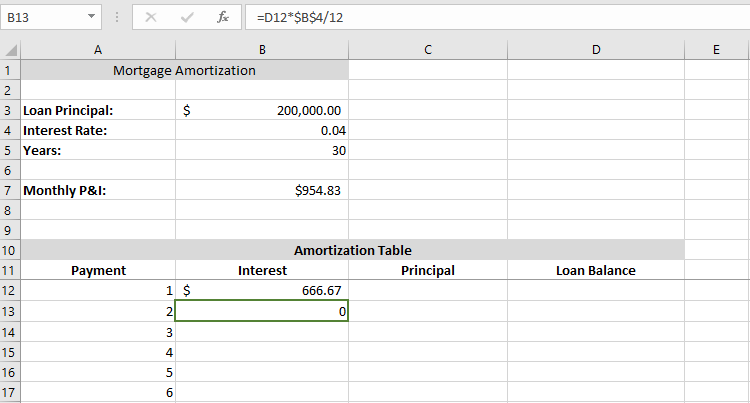
\includegraphics[width=0.75\textwidth]{ExcelAmortizationInterestCalculation}
\end{center}

\paragraph{What's with the dollar signs in B4?} Notice that instead of using B4 in the interest calculation, we are using \$B\$4.  The reason for this is that as we drag our formula down, Excel assumes that we want all of the cells in our formula to move in the same way.  This is, in fact, what we want to happen with the D12 in the formula; the next row should use D13, and so on.  To tell Excel to keep using the value in B4 even as we drag the formula down, you need to use these dollar signs.  You can insert them manually, or press F4 after clicking on the cell number in the formula.\\

The last two calculations are the principal and the loan balance: the principal payment will be the total monthly payment (\$B\$7) minus the interest payment, and the loan balance will be the previous balance minus the principal payment for the current month.
\begin{center}
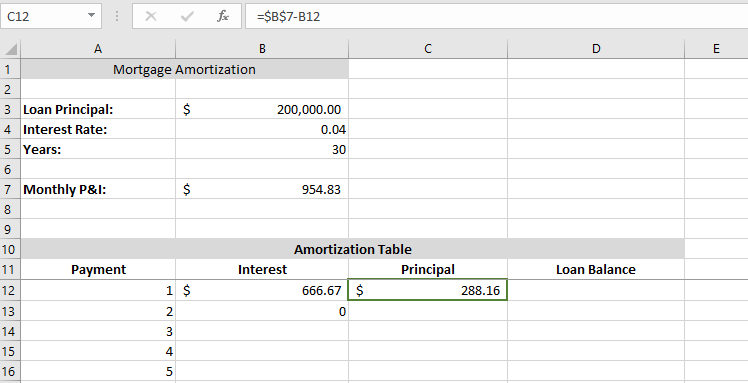
\includegraphics[width=0.75\textwidth]{ExcelAmortizationPrincipalCalculation}
\end{center}

After filling out the first two rows, you should have the following.  Notice that we did the first two rows manually because the first row uses the starting balance several times, which is not consistent with the formula we want to copy.
\begin{center}
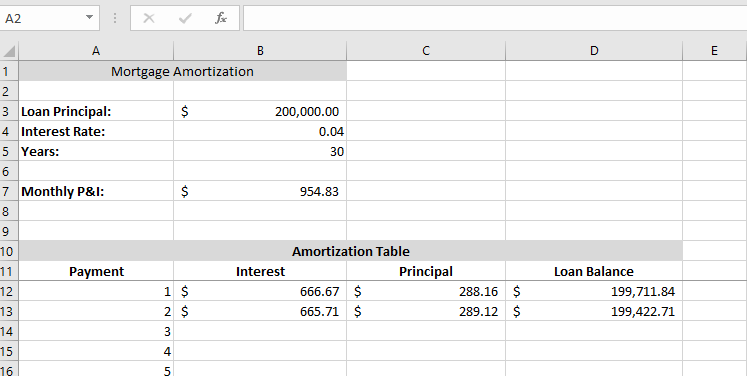
\includegraphics[width=0.75\textwidth]{ExcelAmortizationFirstTwoRows}
\end{center}
\pagebreak

The formulas we want to copy down are the ones in the second row (cells B13 through D13), so if we select those cells and drag downward all the way to payment 360, we'll get the full table:
\begin{center}
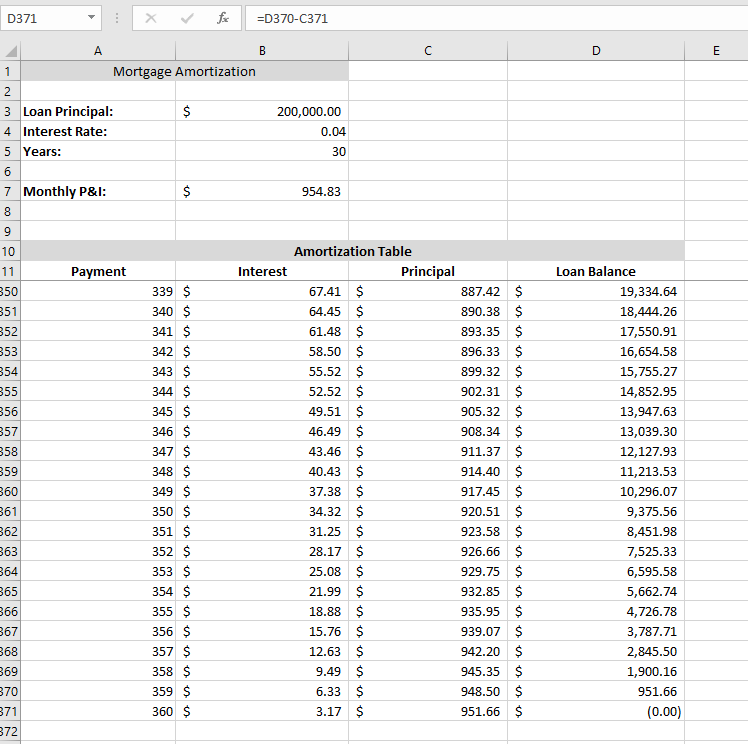
\includegraphics[width=0.75\textwidth]{ExcelAmortizationFullTable}
\end{center}

This shows the end of the table, where the loan balance finally drops to \$0.00.

\subsection{Credit Cards}
So far, we've dealt with \textit{fixed installment loans}, meaning that a specified amount is loaned and paid back with fixed payments in such a way that the balance goes to zero with the final scheduled payment.

On the other hand, there are \textbf{open-ended installment loans}, which require a variable payment each month, and the loan has no guaranteed end date; payments are made for as long as necessary to pay off the loan.  The most common example is a credit card, where the total balance does not have to be paid off each month, and any unpaid balance rolls over to the following month.  Of course, credit card companies take advantage of the ease of payment to rack up huge interest charges---credit card interest rates are among the highest you'll likely see.  If, on the other hand, you pay off the entire balance each month, treating the card more like a debit card, you'll never pay any interest charges to your credit card company.
\begin{center}
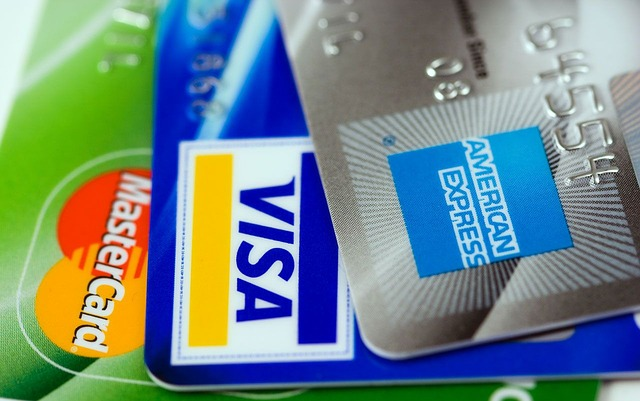
\includegraphics[scale=0.25]{CreditCards1}
\end{center}

\paragraph{Average Daily Balance Method} Different credit card companies calculate interest in different ways, all using the simple interest formula ($I=Prt$).  The difference lies in how $P$ is calculated; since the balance is constantly changing all month, they need a way to combine this all into a single principal.  The method we'll illustrate is called the \textit{average daily balance method}, which as the name suggests, takes the average of the balance on each day of the month.  Thus, if the balance was \$100 on the first 15 days of the month and \$200 on the last 15 days, the average daily balance will be \$150.
\vfill
\pagebreak

To find the average daily balance, add up the balance for each day and divide by the number of days.  In practice, we'll use a table to simplify the calculations by multiplying each different balance by the number of days that the card carried that balance.

\begin{example}[https://www.youtube.com/watch?v=ZUEQu_e2TqY]{Credit Card Charges}
Suppose your VISA card calculates interest using the average daily balance method, and the monthly interest rate is 1.5\% (notice that this means that the nominal annual rate is $1.5\% \times 12 = 18\%$, which is not at all unusually high for a credit card).  The itemized billing for the month of December is shown below.
\begin{center}
\begin{tabular}{l l l}
Detail & Date & Amount\\
\hline
Unpaid balance & December 1 & \$1500\\
Payment received & December 4 & \$300\\
Groceries & December 8 & \$125\\
Gas & December 15 & \$45\\
Wendy's & December 22 & \$8.50\\
Last day of billing period & December 31 &\\
Payment Due Date & January 7 &\\
\end{tabular}
\end{center}

\begin{enumerate}[(a)]
\item Find the average daily balance.
\item Find the interest due for December.
\item Find the total balance owed on the last day of the billing period.
\item This credit card requires a \$15 minimum monthly payment or $1/36$ of the amount due, whichever is higher.  What is the minimum monthly payment due by January 7?
\end{enumerate}

\sol
\begin{enumerate}[(a)]
\item Find the average daily balance.

To do this, we'll build a table to keep track of the unpaid balance after each transaction, and how long that unpaid balance lasts.

\begin{center}
\begin{tabular}{l l}
Date & Unpaid Balance\\
\hline
December 1 & \$1500\\
December 4 & \$1200\\
December 8 & \$1325\\
December 15 & \$1370\\
December 22 & \$1378.50\\
\end{tabular}
\end{center}

Now calculate how many days each balance lasted and multiply the balance by the number of days it lasted; this lets us quickly add up the balance for each day so that we can find the average by dividing this by the number of days.
\begin{center}
\begin{tabular}{l l p{0.7in} p{1.5in}}
Date & Unpaid Balance & Number of Days & (Unpaid balance) $\times$ (Number of Days)\\
\hline
December 1 & \$1500 & 3 & \$4500\\
December 4 & \$1200 & 4 & \$4800\\
December 8 & \$1325 & 7 & \$9275\\
December 15 & \$1370 & 7 & \$9590\\
December 22 & \$1378.50 & 10 & \$13,785\\
\hline
\textbf{Total:} & & 31 & \$41,950
\end{tabular}
\end{center}

The average daily balance is then the sum of the daily balances divided by 31, the number of days in the billing period:
\[\dfrac{\$41,950}{31} = \boxed{\$1353.23}\]

\item Find the interest due for December.

Use the simple interest formula, noting that since the interest rate is given as a \textit{monthly} rate, $t=1$ since we're dealing with a single month:
\[I=Prt = (\$1353.23)(0.015)(1) = \boxed{\$20.30}\]

\item Find the total balance owed on the last day of the billing period.

This is the final balance plus the interest charges:
\[\$1378.50 + \$20.30 = \boxed{\$1398.80}\]

\item This credit card requires a \$15 minimum monthly payment or 1/36 of the amount due, whichever is higher.  What is the minimum monthly payment due by January 7?

Since 1.36 of the amount due is $\$1398.80/36 = \$38.86$, which is more than \$15, the minimum payment due will be $\boxed{\$38.86}$
\end{enumerate}
\end{example}

\begin{try}
Suppose your VISA card calculates interest using the average daily balance method, and the monthly interest rate is 1.8\%.  The itemized billing for the month of May is shown below.
\begin{center}
\begin{tabular}{l l l}
Detail & Date & Amount\\
\hline
Unpaid balance & May 1 & \$850\\
Payment received & May 5 & \$200\\
Groceries & May 7 & \$240\\
Gas & May 13 & \$33\\
Jewelry Store & May 25 & \$575\\
Last day of billing period & May 31 &\\
Payment Due Date & June 7 &\\
\end{tabular}
\end{center}

\begin{enumerate}[(a)]
\item Find the average daily balance.
\item Find the interest due for this month.
\item Find the total balance owed on the last day of the billing period.
\item This credit card requires a \$20 minimum payment or 1/24 of the amount due, whichever is higher.  What is the minimum monthly payment due for this month?
\end{enumerate}
\end{try}

We'll finish this discussion by taking another look at the trap of the minimum payment; we'll use the numbers from the preceding example.  A minimum payment of \$38.84 on a balance of \$1398.13 sounds pretty reasonable, but think about how long it would take to pay off this balance by only making the minimum payment each month (even without adding further charges), since the majority of the minimum payment will go toward interest.

Skipping over the details (this can be figured out using a simple spreadsheet), if you started with a balance of \$1398.13 and never added another charge, just making the minimum payment each month, it would take 123 months to pay it off, or over 10 years.  In doing so, you would end up paying a total of \$2571.46, or nearly twice what you owed.  The lesson is simple: pay off your credit card in full as much as possible, and don't live beyond your means in a way that requires the use of credit to get by.
\begin{exercises}
\ptwo{If you take out an auto loan of \$8500 at 5\% interest for 48 months, what will your monthly payment be?}
\ptwo{If you borrow \$13,000 to buy a boat, and the bank charges 7\% interest for 72 months, how much will you have to pay each month?}

\ptwo{Janine bought \$3000 of new furniture on credit.  Because her credit score isn't very good, the store is charging her a fairly high interest rate on the loan: 16\%.  If she agreed to pay off the furniture over two years, how much will she have to pay each month?}
\ptwo{Carly financed a new \$1200 television at 12\% for 48 months.  How much will she have to pay every month to pay this off?}

\ptwo{If you want to buy a car, and you can afford a monthly payment of \$175, how large of a loan can you get at 4.8\% interest over 60 months?}
\ptwo{Mary is going to finance new office equipment at a 2\% rate over a 4 year term.  If she can afford monthly payments of \$100, how much can she pay for the new office equipment?}

\ptwo{If you buy a \$33,000 car for \$1000 down and monthly payments of \$685 for 60 months, how much will you pay in total for the car?}
\ptwo{A car costs \$27,000, and you're offered a loan that requires \$800 down and a monthly payment of \$575 for 60 months, how much will you pay in interest?}

\ptwo{A car dealership offers a loan with 3.5\% interest for 60 months, and you plan to purchase a car for \$18,000.  You can afford a down payment of \$2500.
\begin{enumerate}[(a)]
\item What will your monthly payment be?
\item How much will you pay in total for the car?
\item How much will you pay in interest over the life of the loan?
\end{enumerate}}
\ptwo{You plan to purchase a \$21,000 car, and your bank offers you a loan at 4.5\% interest for 48 months.  You can afford a down payment of \$4000.
\begin{enumerate}[(a)]
\item What will your monthly payment be?
\item How much will you pay in total for the car?
\item How much will you pay in interest over the life of the loan?
\end{enumerate}}

\ptwo{You want to buy a \$200,000 home, and you have \$40,000 saved up.  The bank offers a 30-year mortgage at 3.8\% interest.
\begin{enumerate}[(a)]
\item If you expect to pay \$6000 in closing costs, what percentage down payment can you afford?
\item If you put less than 20\% down, you'll need to pay mortgage insurance.  Will you require mortgage insurance?
\item What will the principal be on the loan?
\item What will your monthly P\&I payment be?
\item In addition to principal and interest, the property taxes will be 1.5\% of the home value per year, homeowners insurance will be \$750 per year, and the mortgage insurance (if needed, according to part (b)) will be \$25 per month.  What will your total monthly payment amount be?
\item How much will you pay in total over 30 years in principal and interest?
\item How much interest will you pay in total?
\end{enumerate}}
\ptwo{You want to buy a \$375,000 home, and you have \$84,000 saved up.  The bank offers a 20-year mortgage at 3.2\% interest.
\begin{enumerate}[(a)]
\item If you expect to pay \$8000 in closing costs, what percentage down payment can you afford?
\item If you put less than 20\% down, you'll need to pay mortgage insurance.  Will you require mortgage insurance?
\item What will the principal be on the loan?
\item What will your monthly P\&I payment be?
\item In addition to principal and interest, the property taxes will be 1.5\% of the home value per year, homeowners insurance will be \$825 per year, and the mortgage insurance (if needed, according to part (b)) will be \$30 per month.  What will your total monthly payment amount be?
\item How much will you pay in total over 20 years in principal and interest?
\item How much interest will you pay in total?
\end{enumerate}}

\ptwo{You can afford a \$900 per month mortgage payment.  You've found a 30-year loan at 4\% interest.
\begin{enumerate}[(a)]
\item How big of a loan can you afford?
\item How much total money will you pay the bank?
\item How much of that money is interest?
\end{enumerate}}
\ptwo{You can afford a \$1790 per month mortgage payment.  You've found a 15-year loan at 3.25\% interest.
\begin{enumerate}[(a)]
\item How big of a loan can you afford?
\item How much total money will you pay the bank?
\item How much of that money is interest?
\end{enumerate}}

\pthree{If the interest rate on a 30-year mortgage for \$175,000 were changed from 3.8\% to 3.1\%, how much would you save over the life of the loan?}
\pthree{How much would you save (over the life of the loan) on a 20-year mortgage at 4.5\% if you reduced the amount you borrowed from \$300,000 to \$260,000?}
\pthree{If you borrow \$250,000, how much could you save over the life of the loan if you took out a 15-year mortgage at 4.5\% instead of a 30-year mortgage at 4\%?}

\pone{Suppose you take out a \$315,000 mortgage for 30 years at 4.5\% interest.
\begin{enumerate}[(a)]
\item Find the monthly payment on this mortgage.
\item Fill out the first two rows of the amortization schedule below.
\begin{center}
\begin{tabular}{|>{\centering\arraybackslash\hspace{0pt}}p{1.1in} | >{\centering\arraybackslash\hspace{0pt}}p{1.1in} | >{\centering\arraybackslash\hspace{0pt}}p{1.2in} | >{\centering\arraybackslash\hspace{0pt}}p{1in}|}
\hline
{\small Payment Number} & {\small Interest Payment} & {\small Principal Payment} & {\small Balance of Loan}\\
\hline
1 & & & \\
\hline
2 & & & \\
\hline
& & &
\end{tabular}
\end{center}
\end{enumerate}}

\pone{Suppose you take out a \$180,000 mortgage for 15 years at 3.7\% interest.
\begin{enumerate}[(a)]
\item Find the monthly payment on this mortgage.
\item Fill out the first two rows of the amortization schedule below.
\begin{center}
\begin{tabular}{|>{\centering\arraybackslash\hspace{0pt}}p{1.1in} | >{\centering\arraybackslash\hspace{0pt}}p{1.1in} | >{\centering\arraybackslash\hspace{0pt}}p{1.2in} | >{\centering\arraybackslash\hspace{0pt}}p{1in}|}
\hline
{\small Payment Number} & {\small Interest Payment} & {\small Principal Payment} & {\small Balance of Loan}\\
\hline
1 & & & \\
\hline
2 & & & \\
\hline
& & &
\end{tabular}
\end{center}
\end{enumerate}}

\ptwo{Suppose your VISA card calculates interest using the average daily balance method, and the monthly interest rate is 1.4\%.  The itemized billing for the month of April is shown below.\\

\begin{tabular}{l l l}
Detail & Date & Amount\\
\hline
Unpaid balance & April 1 & \$1100\\
Payment received & April 3 & \$500\\
New computer & April 11 & \$750\\
Books & April 15 & \$65\\
Mattress & April 28 & \$600\\
Last day of billing period & April 30 &\\
Payment Due Date & May 7 &\\
\end{tabular}

\begin{enumerate}[(a)]
\item Find the average daily balance.
\item Find the interest due for this month.
\item Find the total balance owed on the last day of the billing period.
\item This credit card requires a \$20 minimum payment or 1/36 of the amount due, whichever is higher.  What is the minimum monthly payment due for this month?
\end{enumerate}}
\ptwo{Suppose your MasterCard calculates interest using the average daily balance method, and the monthly interest rate is 2.1\%.  The itemized billing for the month of August is shown below.\\

\begin{tabular}{l l l}
Detail & Date & Amount\\
\hline
Unpaid balance & August 1 & \$300\\
Payment received & August 9 & \$100\\
Tuition & August 10 & \$4500\\
Textbooks & August 18 & \$350\\
Groceries & August 25 & \$180\\
Last day of billing period & August 31 &\\
Payment Due Date & September 7 &\\
\end{tabular}

\begin{enumerate}[(a)]
\item Find the average daily balance.
\item Find the interest due for this month.
\item Find the total balance owed on the last day of the billing period.
\item This credit card requires a \$15 minimum payment or 1/24 of the amount due, whichever is higher.  What is the minimum monthly payment due for this month?
\end{enumerate}}
\vfill
\pagebreak

\pone{\textbf{Project: Finding a Mortgage}

You and your family are looking to move and are shopping for a house.  Your job is to find a mortgage that you can afford.

You may choose your family size---you can be married with kids, married without kids, or single.  You may also pick anywhere in the country that you'd like to live, but you can only make the median income listed for the state you choose.  If you are married, you can assume that both you and your spouse are working and each are paid the median income for that state.

\begin{enumerate}[(a)]
\item Decide where you want to live.  Do some research and find the median income for that state, and decide whether you are single or married, and whether or not you have children.
\item Search \href{http://www.realtor.com}{realtor.com} or a similar website to find a house that fits your family's needs.  Take note of the
\begin{itemize}
\item List price of the home.
\item Property taxes listed under the ``Property History'' tab.  If property taxes are not listed, estimate the annual property taxes as 2\% of the purchase price.
\end{itemize}
\item Estimate the down payment you can afford, and take note of the principal of the loan that you will need.
\item Do some research to find current interest rates.  Use \href{http://www.bankrate.com}{bankrate.com} or a similar website to find mortgage rates (make sure to find a mortgage without \emph{points}).  Find three options: mortgages for 30 years, 20 years, and 15 years.
\begin{itemize}
\item What is the monthly payment for each option?
\item How much will you pay in total for principal and interest over the life of the loan for each option?
\item Keeping your monthly budget in mind, which option will you choose?
\end{itemize}

\item Complete the following steps to find if you can afford this home.  This worksheet uses a typical rule of thumb that you should not spend more than 28\% of your income on housing.
\begin{center}
\begin{tabular}{p{3.75in} p{3in}}
\textbf{Monthly Gross Income} &\\
\hspace{0.5in} Borrower's annual income & $\$ \line(1,0){150}$\\
& \\
\hspace{0.5in} Co-borrower's annual income & $+ \line(1,0){150}$\\
& \\
\hspace{0.5in} Total gross annual income & $\$ \line(1,0){150}$\\
\hspace{0.75in} Divide total gross income by 12 & \hspace{0.25in} $\div$ 12\\
& \\
\hspace{0.5in} Total monthly gross income & $\$ \line (1,0){150}$\\
\hspace{0.75in} Find 28\% of this & \hspace{0.25in} $\times 0.28$\\
& \\
\hspace{0.5in} \textbf{Allowable monthly housing cost} & $\$\line(1,0){150}$ (A)\\
& \\
\textbf{Monthly Taxes} &\\
\hspace{0.5in} Home purchase price & $\$ \line(1,0){150}$\\
& \\
\hspace{0.5in} Estimated taxes & $\$ \line(1,0){150}$\\
\hspace{0.75in} Divide taxes by 12 & \hspace{0.25in} $\div 12$\\
& \\
\hspace{0.5in} Monthly taxes & $\$ \line(1,0){150}$ (B)\\
& \\
\textbf{Monthly Housing Cost} & \\
\hspace{0.5in} Monthly mortgage payment & $\$ \line(1,0){150} \ +$\\
& \\
\hspace{0.5in} Estimated monthly taxes (B) & $\$ \line(1,0){150} \ +$\\
& \\
\hspace{0.5in} Condo or homeowner's fee (if applicable) & $\$ \line(1,0){150}$\\
& \\
\textbf{Total Monthly Housing Cost} & $= \$ \line(1,0){140}$ (C)
\end{tabular}
\end{center}
Compare (A) and (C).  Can you afford the house you want to buy?  If not, choose a less expensive house and redo this project.
\end{enumerate}}

\end{exercises}

\section{Income Tax}
\setcounter{ExampleCounter}{1}
\marginnote{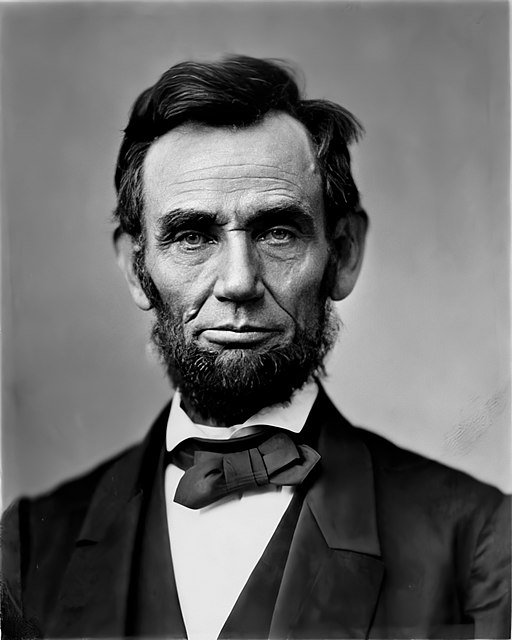
\includegraphics[width=1.5in]{AbrahamLincoln}}
Before the Civil War, there was no federal income tax in the United States.  At the beginning of the war, to help pay for it, Congress passed the Revenue Act of 1861, which imposed a tax of 3\% on all incomes over \$800.  The following year, the Revenue Act of 1862 instituted a 3\% tax on incomes over \$600 and 5\% on incomes over \$10,000.  These taxes were repealed after the war, and it wasn't until the ratification of the Sixteenth Amendment in 1913 that a federal income tax was finally established for good.\\

Interestingly, these two laws passed by Congress in 1861 and 1862 introduce us to one of the main distinctions between types of taxes; specifically, they give us examples of \textbf{flat} taxes and \textbf{progressive} taxes.\\

\textbf{Flat taxes}--like sales tax, property tax, or gasoline tax--are calculated as a single percentage of a total.

\begin{example}[https://www.youtube.com/watch?v=QjjpqBp5d6w]{Property Taxes}
Joan paid \$3,200 in property taxes on her house, which was valued at \$215,000 last year.  What is the property tax rate?

\sol
The equivalent percentage is \[\dfrac{3,200}{215,000} = 0.01488 = \boxed{1.49\%}\]
\end{example}

In the section on Applied Percentage Problems, we worked out examples involving sales tax; all you need to know is the total charge before taxes and the tax rate, and you can calculate the sales tax by multiplying these.

\textbf{Progressive taxes}--like the current federal income tax--are calculated using different tax rates for different income levels.  Specifically, the term \emph{progressive} means that tax rates increase for higher income levels.  A tax that did the opposite (lowered tax rates for higher incomes) would be called a \emph{regressive tax}; these are not generally used in practice, but you may hear this term, for instance, to describe lottery tickets, since they are bought more frequently by people on the lower end of the income scale.

\begin{formula}{Tax Categories}
\begin{itemize}
\item \marginnote{ex: sales tax}A \textbf{flat tax} charges a consistent percentage, no matter what the taxed amount is.
\item \marginnote{ex: income tax}A \textbf{progressive tax} charges a higher percentage for higher taxed amounts.
\end{itemize}
\end{formula}

The two bills passed by Congress during the Civil War are examples of these two categories.  The tax created in 1861 was a flat tax, although technically it could be regarded as a progressive tax with a tax rate of 0\% for all incomes under \$800.  But income tax was incredibly simple to calculate: simply subtract \$800 from your annual income, and multiply the result by 3\%.

The 1862 tax was a progressive tax with two different tax rates depending on income.

\subsection{Progressive Taxes: Income Tax}
This brings us to the key feature of the calculations we'll be doing in this calculation: \textbf{the progressive tax rates do not apply to \emph{all} of your income}.  Instead, a taxpayer's income is split into segments, and each segment is taxed at the rate that applies to it.

Let's use the 1862 tax to illustrate a simple example.  Remember that incomes over \$600 were taxed at 3\% and incomes over \$10,000 were taxed at 5\%.

For comparison, consider three people:
\begin{enumerate}
\item Mary is a schoolteacher, earning \$360 a year
\item John is a schoolteacher, earning \$846 a year
\item William is a member of Congress and a businessman, with a total income of \$12,000
\end{enumerate}

Now calculate how much each owes in taxes:
\begin{enumerate}
\item Since Mary makes less than \$600 a year, she owes no taxes.
\item Since John earns more than \$600, but less than \$10,000, only the first tax rate applies to him.  However, \emph{only his income over \$600} gets taxed.  This means that he's only taxed on \$246, and 3\% of \$246 is \$7.38, so that's John's full tax bill.
\item William makes more than \$10,000, so both tax rates apply to him.  Just like John, his first \$600 are not taxed at all.  At that point, his income is taxed at 3\% all the way from dollar 600 up to dollar 10,000, and everything beyond that is taxed at 5\%.

It may be simplest to start at the top: he has \$2,000 past the \$10,000 threshold, so that amount is taxed at 5\%: $(5\%)(\$2000) = \$100$.  Then from the \$10,000 mark down to the \$600 mark represents a total of \[\$10,000 - \$600 = \$9400\] which is taxed at 3\%:
\[(3\%)(\$9400) = \$282.\]

William's total tax bill, then, is the sum of these two, for a total of \$382.
\end{enumerate}

It can help to think of a person's income as if they are holding dollar bills, and placing their money into a series of buckets.  The first bucket (in the example above) can hold \$600, so once that's been filled, the person starts putting their money in the next bucket, which can hold \$9400, and so on.  Once the person has finished splitting their money this way, a certain percentage of each bucket is removed, and they can keep the rest.\\

If you've heard the term \textbf{tax brackets}, it refers to this progressive pattern.  Usually, if someone mentions what tax bracket they belong to, they really mean the highest bucket that they reach, but crucially, \emph{not all of their income is taxed at that rate}.  Whether you make \$40,000 or \$4,000,000 a year, your first dollar will be taxed at the same rate.

\subsection{Using Modern Tax Rates}
Let's take the example of someone who makes \$82,350 this year (using 2020, the year of publication).  In 2020, a single taxpayer's first \$9,875 are taxed at 10\%, everything from that point to \$40,125 is taxed at 12\%, and from that point to \$85,525 is taxed at 22\%.  We can summarize this with a table like the one below.
\begin{center}
\begin{tabular}{l l}
\textbf{Tax Rate} & \textbf{Income}\\
10\% & up to \$9,875\\
12\% & \$9,875 to \$40,125\\
22\% & \$40,125 to \$85,525
\end{tabular}
\end{center}
There's more to this table, but that's as far as we need to go, since our fictional taxpayer doesn't make more than \$85,525.

\begin{center}
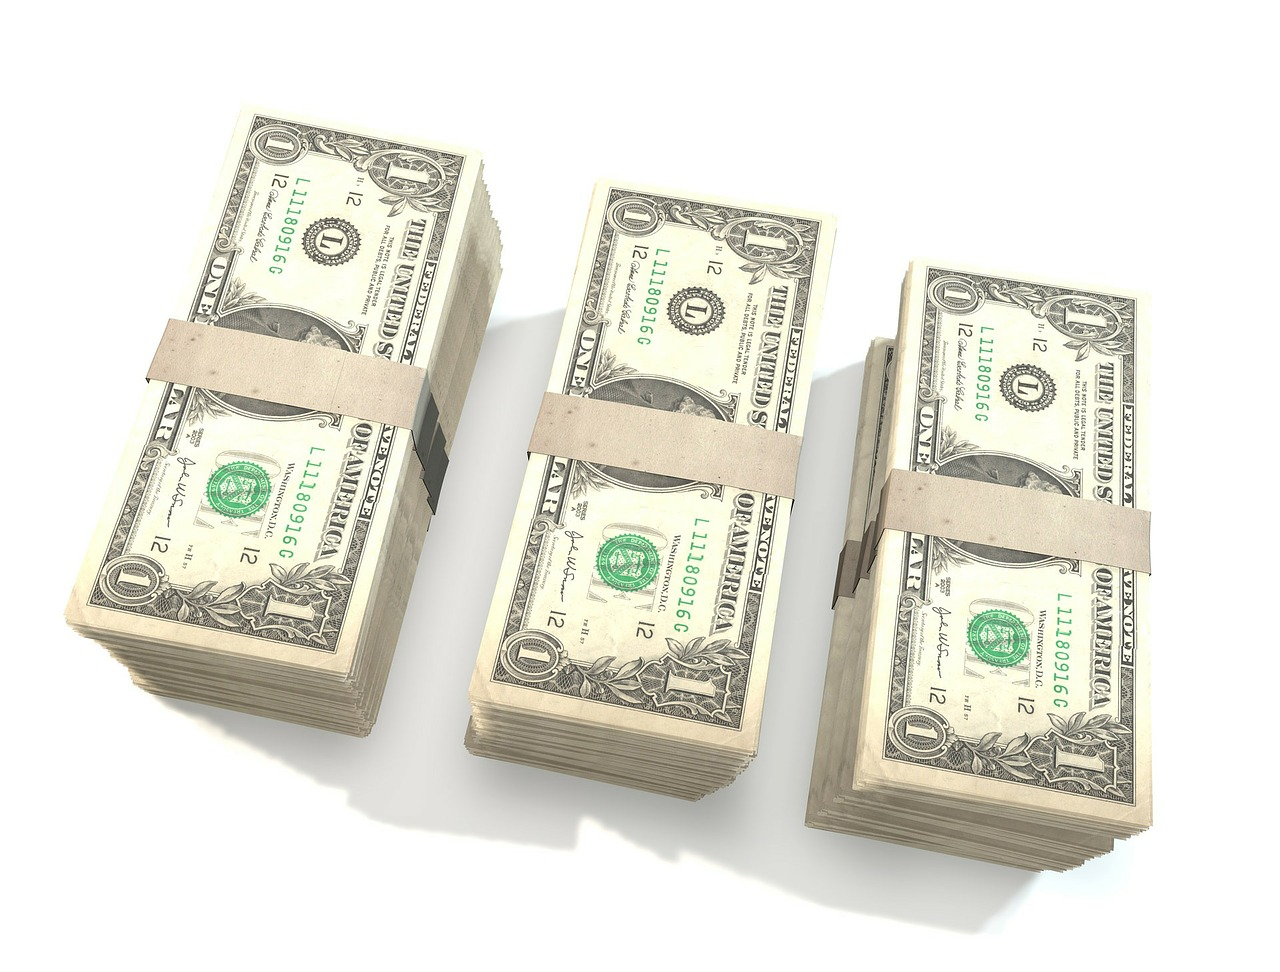
\includegraphics[scale=0.07]{Dollars1}

\begin{tcolorbox}[colframe=green!5,colback=green!5,sharp corners=all]
\begin{center}
\$82,350

$\overbrace{
\begin{tabular}{r | c c c}
& & & \\
\marginnote{Split money into brackets}Dollars & 1 -- 9,875 & 9,876 -- 40,125 & 40,126 -- 82,350\\
& & & \\
Tax Rate & 10\% & 12\% & 22\%\\
& & & \\
\marginnote{Multiply the amount in each }Calculation & \$9,875(0.1) & (\$40,125 -- \$9,875)(0.12) & (\$82,350 -- \$40,125)(0.22)\\
& & & \\
\marginnote{bracket by the tax rate}& = \$987.50 & = \$3,630.00 & = \$9,289.50
\end{tabular}
}$
\vspace{0.25in}

This taxpayer pays $\$987.50 + \$3,630.00 + \$9,289.50 = \$13,907$ in taxes.

\end{center}
\end{tcolorbox}
\end{center}

The tax rates for each bracket may change from year to year, but the process remains the same:
\begin{enumerate}
\item Divide the taxable income into these brackets, putting each dollar into the appropriate bracket until you get to the end of the income (so if the taxpayer's income in the example above was \$32,000, we would have stopped in the second bracket and not spilled over into the third).
\item Multiply the amount in each bracket by the tax rate for that bracket.
\item Add up the tax amounts from each bracket to find the total income tax owed.
\end{enumerate}

The following table is the tax table for 2020, showing the tax brackets and associated tax rate for each.
\vspace{0.25in}

\label{Tax Table}
\checkoddpage
\ifoddpage{
\begin{adjustwidth}{-0.25in}{-1.5in}
\begin{center}
\begin{tabular}{| p{1in} | p{1.5in} | p{1.75in} | p{1.5in} |}
\hline
\cellcolor{brown!25}Tax Rate & \cellcolor{brown!25}\parbox{1.3in}{\text{}\\ Single or\\ Married Filing\\ Separately\\ \text{}} & \cellcolor{brown!25}Married Filing Jointly & \cellcolor{brown!25}Head of Household\\
\hline
\cellcolor{brown!25}10\% & up to \$9,875 & up to \$19,750 & up to \$14,100\\
\hline
\cellcolor{brown!25}12\% & \$9,875 to \$40,125 & \$19,750 to \$80,250 & \$14,100 to \$53,700\\
\hline
\cellcolor{brown!25}22\% & \$40,125 to \$85,525 & \$80,250 to \$171,050 & \$53,700 to \$85,500\\
\hline
\cellcolor{brown!25}24\% & \$85,525 to \$163,300 & \$171,050 to \$326,600 & \$85,500 to \$163,300\\
\hline
\cellcolor{brown!25}32\% & \$163,300 to \$207,350 & \$326,600 to \$414,700 & \$163,300 to \$207,350\\
\hline
\cellcolor{brown!25}35\% & \$207,350 to \$518,400 & \$414,700 to \$622,050 & \$207,350 to \$518,400\\
\hline
\cellcolor{brown!25}37\% & more than \$518,400 & more than \$622,050 & more than \$518,400\\
\hline
\cellcolor{brown!25}\parbox{0.9in}{\text{}\\ Standard\\ Deduction\\ \text{}} & \$12,400 & \$24,800 & \$18,650\\
\hline
\end{tabular}
\end{center}
\end{adjustwidth}
\vspace{0.25in}}
\else{\begin{adjustwidth}{-1.75in}{-0.25in}
\begin{center}
\begin{tabular}{| p{1in} | p{1.5in} | p{1.75in} | p{1.5in} |}
\hline
\cellcolor{brown!25}Tax Rate & \cellcolor{brown!25}\parbox{1.3in}{\text{}\\ Single or\\ Married Filing\\ Separately\\ \text{}} & \cellcolor{brown!25}Married Filing Jointly & \cellcolor{brown!25}Head of Household\\
\hline
\cellcolor{brown!25}10\% & up to \$9,875 & up to \$19,750 & up to \$14,100\\
\hline
\cellcolor{brown!25}12\% & \$9,875 to \$40,125 & \$19,750 to \$80,250 & \$14,100 to \$53,700\\
\hline
\cellcolor{brown!25}22\% & \$40,125 to \$85,525 & \$80,250 to \$171,050 & \$53,700 to \$85,500\\
\hline
\cellcolor{brown!25}24\% & \$85,525 to \$163,300 & \$171,050 to \$326,600 & \$85,500 to \$163,300\\
\hline
\cellcolor{brown!25}32\% & \$163,300 to \$207,350 & \$326,600 to \$414,700 & \$163,300 to \$207,350\\
\hline
\cellcolor{brown!25}35\% & \$207,350 to \$518,400 & \$414,700 to \$622,050 & \$207,350 to \$518,400\\
\hline
\cellcolor{brown!25}37\% & more than \$518,400 & more than \$622,050 & more than \$518,400\\
\hline
\cellcolor{brown!25}\parbox{0.9in}{\text{}\\ Standard\\ Deduction\\ \text{}} & \$12,400 & \$24,800 & \$18,650\\
\hline
\end{tabular}
\end{center}
\end{adjustwidth}
\vspace{0.25in}}
\fi

Note that there is an extra row at the bottom that describes the \emph{standard deduction}; we'll discuss that shortly.  Also, the term ``Head of Household'' may be confusing, but it simply means a single individual with one or more dependents.

\begin{example}[https://www.youtube.com/watch?v=p7ofzArnTxo]{Income Tax}
Using the tax table above, how much would a married taxpayer who files separately from their spouse owe on a taxable income of \$98,400?

\sol
First, note that we'll be using the first column, since this taxpayer is married, filing separately.  Next, divide the \$98,400 into the appropriate brackets:

\begin{center}
\$98,400

$\overbrace{
\begin{tabular}{r | c c c c}
& & & \\
Dollars & 1 -- 9,875 & 9,876 -- 40,125 & 40,125 -- 85,525 & 85,525 -- 98,400\\
& & & \\
Tax Rate & 10\% & 12\% & 22\% & 24\%\\
\end{tabular}
}$
\end{center}

Then simply multiply the amount in each bracket by that tax rate and add up these totals:
\begin{align*}
\textrm{Tax Owed } &= (9,875)(0.1) + (40,125-9,875)(0.12)\\ &\hspace{0.5in} + (85,525-40,125)(0.22) + (98,400-85,525)(0.24)\\ &= \boxed{\$17,695.50}
\end{align*}

Notice that the \emph{effective tax rate} for this taxpayer (the percentage of their taxable income that they actually paid) was
\[\dfrac{\$17,695.50}{\$98,400.00} = 0.1798\] or about 18\%.
\end{example}

\begin{try}
Using the 2020 tax table, how much would a head of household owe on a taxable income of \$47,000?
\end{try}

\subsection{Deductions and Credits}
We've used the term \textbf{taxable income} several times; what does that mean?\\

It turns out that you won't be taxed on your full income; by law, there are ways that you can reduce your tax burden, and broadly speaking, these fall into two categories: \textbf{deductions} and \textbf{credits}.

\paragraph{Warning:} You should know that the rest of this discussion presents a simplified view; if you study accounting, for instance, you'll find that we're glossing over many of the fine details here.  The goal of this section is not to prepare you for the CPA exam, but simply to give you a broad understanding of how taxes are calculated.\\

\begin{formula}{Deductions and Credits}
Tax deductions and credits are both designed to reduce the amount of income a taxpayer owes.  The difference between them is when they are applied.\\

\textbf{Tax Deductions} are subtracted from the taxpayer's \emph{gross income}, which is the total amount of income they receive in a year.  By subtracting these, the taxable income is reduced, which ultimately results in a lower tax calculation.\\

\textbf{Tax Credits} are subtracted \emph{after} calculating taxes; i.e. they are subtracted from the tax owed, as determined using the tax table.
\end{formula}

Tax credits have a more direct impact on the tax owed, but deductions are more common.

\paragraph{Examples of Deductions and Credits:} Common tax deductions include things like
\begin{itemize}
\item Interest paid on a mortgage
\item Contributions to a traditional IRA (since traditional IRAs are taxed in retirement)
\item Charitable contributions
\item Education expenses
\item Self-employment expenses
\end{itemize}
Tax credits include
\begin{itemize}
\item The Lifetime Learning Credit, which rewards undergraduate and graduate study
\item Child tax credit and adoption credit
\item Earned income tax credit, for low- and moderate-income taxpayers
\end{itemize}
There are often short-term tax credits created to incentivize behavior like purchasing electric vehicles or energy-efficient appliances.\\

In visual terms, it all begins with the gross income, the total number for all money coming in from employment, investment returns, side jobs, and so on.  The deductions are removed from this, and the remainder (the taxable income) is split into buckets, according to the tax brackets.
\begin{center}
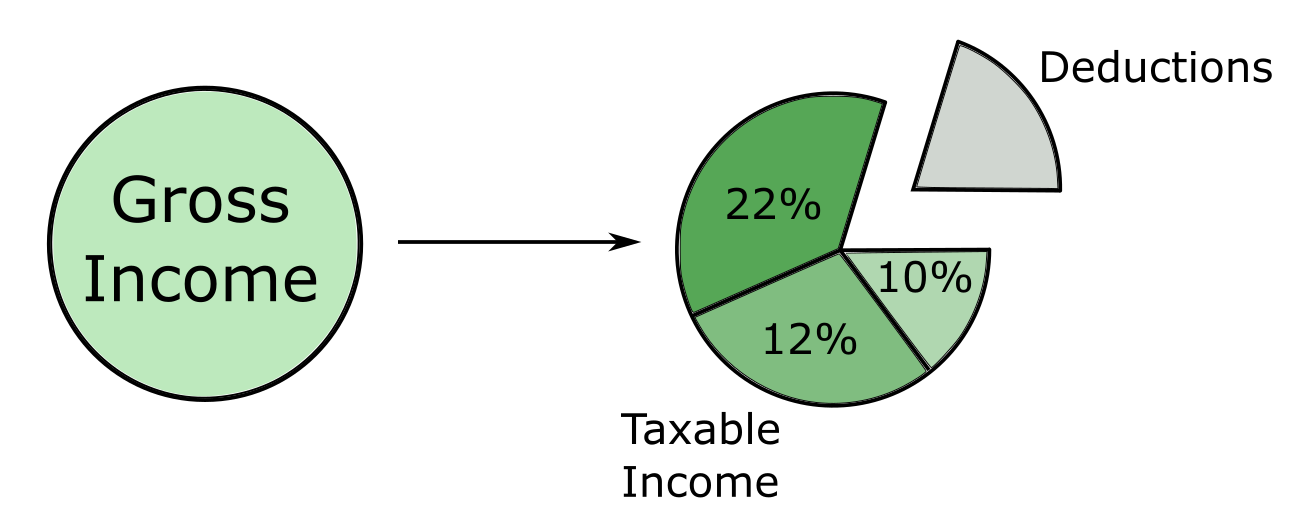
\includegraphics[width=0.6\textwidth]{TaxableIncomeIllustration}
\end{center}
\vfill
\pagebreak

Once the appropriate percentage of each segment has been accounted for, this forms the initial tax calculation, but then any applicable tax credits are subtracted, resulting in the final tax owed.
\begin{center}
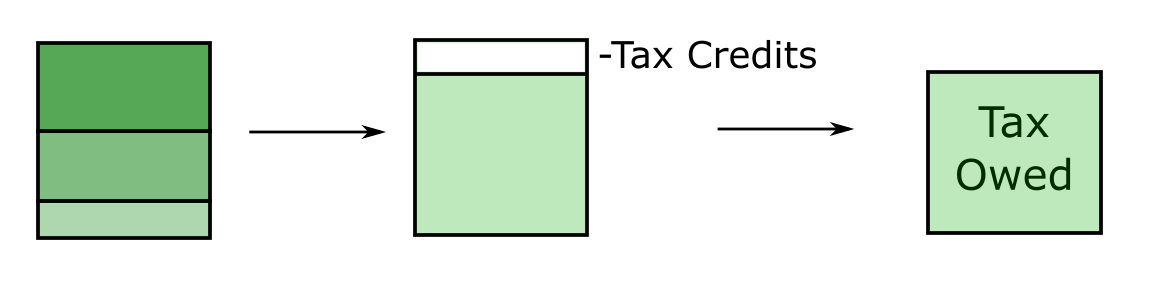
\includegraphics[width=0.6\textwidth]{TaxCreditIllustration}
\end{center}

For instance, if a taxpayer with a gross income of \$50,000 could claim deductions totaling \$13,000 and found \$500 worth of tax credits, it would work out something like this:
\begin{itemize}
\item \textbf{Gross Income:} \$50,000
\item \textbf{Taxable Income:} (subtract the deductions) \$50,000 - \$13,000 = \$37,000
\item \textbf{Initial Tax:} (skipping the calculation, but use the tax table) \$4242.50
\item \textbf{Final Tax Owed:} (subtract the credits) \$4242.50 - \$500 = \$3742.50
\end{itemize}
This person would owe a final tax bill of \$3742.50.\\

That's the basics of deductions and credits, but there's one final piece to the puzzle that we need to understand: \textbf{itemized} deductions vs. the \textbf{standard} deduction.

\begin{formula}{Standard and Itemized Deductions}
Taxpayers can choose to either take the standard deduction (listed on the tax table) or itemize their deductions (add up all the deductions that apply to them).\\

In practice, a taxpayer will add up the itemized deductions, and if this total is larger than the standard deduction, they will choose to go the itemized route.  If not, they will choose to use the standard deduction.
\end{formula}

Basically, there's a minimum deduction amount; if you find that your itemized deductions surpass that, you can use this larger sum as your deduction total.\\

With that, we're ready to work out a full example.
\begin{example}{Tax Calculation}
Use the 2020 tax table on page \pageref{Tax Table} to calculate the final tax owed by a single taxpayer whose details are given below.
\begin{center}
\begin{tabular}{r l}
Gross income: & \$65,000\\
Deductions: & \$3000: charitable donations\\
& \$6000: contribution to traditional IRA\\
& \$1500: education expenses\\
& \$300: cost of tax preparation\\
Tax credit: & \$500: energy-efficient appliances
\end{tabular}
\end{center}

\sol
First, decide whether this person will use itemized deductions or the standard deduction:
\begin{align*}
\marginnote{Calculate deductions}
\textrm{Itemized deductions } &= \$3000 + \$6000 + \$1500 + \$300\\
&= \$10,800
\end{align*}
Since the standard deduction for a single taxpayer (\$12,400) is larger, they will use the standard deduction.\\

Next, subtract the deductions from the gross income to find the taxable income:
\begin{align*}\marginnote{Find the taxable income}
\textrm{Taxable income } &= \textrm{ Gross income } - \textrm{ deductions (standard) }\\
&= \$65,000 - \$12,400\\
&= \$52,600
\end{align*}
\pagebreak

Now divide the taxable income into its brackets and calculate the tax owed from each bracket:
\begin{center}
\$52,600\marginnote{Divide the taxable income into brackets}

$\overbrace{
\begin{tabular}{r | c c c}
& & & \\
Dollars & 1 -- 9,875 & 9,876 -- 40,125 & 40,126 -- 52,600\\
%& & & \\
Tax Rate & 10\% & 12\% & 22\%\\
\end{tabular}
}$
\end{center}
\begin{align*}\marginnote{Multiply the amount in each bracket by that tax rate}
\textrm{Tax Owed } &= (9,875)(0.1) + (40,125-9,875)(0.12)\\ &\hspace{0.5in} + (52,600-40,125)(0.22)\\ &= \$7,362
\end{align*}

Finally, subtract the tax credit from this initial tax calculation to find the final amount that they owe:

\marginnote{Subtract the tax credit}\[\textrm{Final Tax Owed } = \$7,362 - \$500 = \boxed{\$6,872}\]
\end{example}

\begin{try}
Use the 2020 tax table to calculate the tax owed by a married couple filing jointly whose details are given below.
\begin{center}
\begin{tabular}{r l}
Gross income: & \$74,000\\
Deductions: & \$5500: charitable donations\\
& \$150: cost of tax preparation\\
Tax credit: & \$700: child tax credit
\end{tabular}
\end{center}
\end{try}

\checkoddpage
\ifoddpage{
\begin{adjustwidth}{0in}{-1.25in}
\begin{proc}{Tax Withholding}
During World War II, when the U.S. government was in dire need of tax revenue in order to avoid the rampant inflation that occurred during World War I, the IRS began to investigate tax withholding.  Rather than collecting taxes at the end of the year, they began to withhold taxes from workers' paychecks throughout the year, and then make up the difference at the end, either by a refund or an extra tax payment.  Milton Friedman, who won the 1976 Nobel Prize in economics, helped to formulate this plan.\\

New employees fill out a W-4 form, which is intended to calculate as accurately as possible how much they'll owe in taxes, so that the correct amount can be collected.  Many people like the idea of overestimating, because if more is withheld throughout the year, they receive a huge refund check.  However, this is not actually a good policy, since in effect they are giving the government an interest-free loan for the entire year with no strings attached.
\end{proc}
\end{adjustwidth}
} \else{
\begin{adjustwidth}{-1.25in}{0in}
\begin{proc}{Tax Withholding}
During World War II, when the U.S. government was in dire need of tax revenue in order to avoid the rampant inflation that occurred during World War I, the IRS began to investigate tax withholding.  Rather than collecting taxes at the end of the year, they began to withhold taxes from workers' paychecks throughout the year, and then make up the difference at the end, either by a refund or an extra tax payment.  It was Milton Friedman, who won the 1976 Nobel Prize in economics, who helped to formulate this plan.\\

New employees fill out a W-4 form, which is intended to calculate as accurately as possible how much they'll owe in taxes, so that the correct amount can be collected.  Many people like the idea of overestimating, because if more is withheld throughout the year, they receive a huge refund check.  However, this is not actually a good policy, since in effect they are giving the government an interest-free loan for the entire year with no strings attached.
\end{proc}
\end{adjustwidth}
} \fi
\begin{exercises}

\pthree{A \line(1,0){75} \ is a tax at a consistent rate.}
\pthree{A \line(1,0){75} \ is a tax for which the rate increases for higher taxed amounts}
\pthree{A \line(1,0){75} \ is a tax for which the rate decreases for higher taxed amounts}

\pthree{If the property taxes are \$1800 on a home valued at \$140,000, what is the effective tax rate?}
\pthree{In state A, the gas tax is 28 cents per gallon, where the average pre-tax cost of gas is \$2.58 per gallon.  In state B, the gas tax is 25 cents per gallon, where the average pre-tax cost of gas is \$2.50.  Which state has a lower gas tax rate?}
\pthree{If the sales tax is \$16.05 on a purchase of \$214, what is the sales tax rate?}

\ptwo{Using the 2020 tax table on page \pageref{Tax Table}, how much would a single taxpayer owe on a taxable income of \$55,000?}
\ptwo{Using the 2020 tax table on page \pageref{Tax Table}, how much would a married couple filing jointly owe on a taxable income of \$92,000?}

\textit{For problems 9--14, use the marginal tax table on page \pageref{Tax Table} to calculate the tax owed by each taxpayer.}\\
\ptwo{\\
\begin{tabular}{r l}
Taxpayer: & Single\\
Gross income: & \$75,000\\
Deductions: & \$18,000: mortgage interest\\
& \$2500: property taxes\\
& \$2000: charitable donations\\
& \$300: cost of tax preparation\\
Tax credit: & \$800
\end{tabular}}
\ptwo{\\
\begin{tabular}{r l}
Taxpayer: & Single\\
Gross income: & \$40,000\\
Deductions: & \$10,000: mortgage interest\\
& \$2000: property taxes\\
& \$300: charitable donations\\
Tax credit: & \$1300
\end{tabular}}

\ptwo{\\
\begin{tabular}{r l}
Taxpayer: & Married, filing jointly\\
Gross income: & \$85,500\\
Deductions: & \$5000: charitable donations\\
& \$3750: state taxes\\
Tax credit: & \$750
\end{tabular}}
\ptwo{\\
\begin{tabular}{r l}
Taxpayer: & Married, filing jointly\\
Gross income: & \$52,000\\
Deductions: & \$9000: mortgage interest\\
& \$4500: charitable donations\\
& \$1500: theft loss\\
& \$1800: state taxes\\
Tax credit: & \$1400
\end{tabular}}

\ptwo{\\
\begin{tabular}{r l}
Taxpayer: & Head of Household\\
Gross income: & \$104,000\\
Deductions: & \$18,000: mortgage interest\\
& \$5300: property taxes\\
& \$4800: state taxes\\
Tax credit: & none
\end{tabular}}
\ptwo{\\
\begin{tabular}{r l}
Taxpayer: & Head of Household\\
Gross income: & \$43,000\\
Deductions: & \$3700: property taxes\\
& \$3650: state taxes\\
Tax credit: & none
\end{tabular}}
\vfill
\pagebreak

\pone{\textbf{Project: Flat Tax, Modified Flat Tax, and Progressive Tax}

Many people have proposed various revisions to the income tax collection in the U.S.  Some, for example (including Milton Friedman), have claimed that a flat tax would be fairer.  Others call for revisions to how different types of income are taxed.  This project is for you to investigate this idea.\\

Imagine the country is made up of 100 households.  The federal government needs to collect \$800,000 in income taxes to be able to function (this is roughly proportional to the actual U.S. population and tax needs, but using smaller, more manageable numbers).  The population consists of 6 groups:
\begin{center}
\begin{tabular}{r l}
Group A: & 20 households that earn \$12,000 each\\
Group B: & 20 households that earn \$29,000 each\\
Group C: & 20 households that earn \$50,000 each\\
Group D: & 20 households that earn \$79,000 each\\
Group E: & 15 households that earn \$129,000 each\\
Group F: & 5 households that earn \$295,000 each
\end{tabular}
\end{center}
We are going to determine new income tax rates.

\paragraph{Proposal A} The first proposal we'll consider is a flat tax --- one where every income group is taxed at the same percentage rate.
\begin{enumerate}[1)]
\item Determine the total income for the population.
\vspace{1in}

\item Determine what flat tax rate would be necessary to collect enough money.
\vspace{1in}
\end{enumerate}

\paragraph{Proposal B} The second proposal we'll consider is a modified flat-tax plan, where everyone only pays taxes on any income over \$20,000.  So everyone is Group A will pay no taxes, for instance, and everyone in Group B will pay taxes only on \$9,000.
\begin{enumerate}[1)]
\setcounter{enumi}{2}
\item Determine the total \textit{taxable} income for the population.
\vspace{1in}

\item Determine what flat tax rate would be necessary to collect enough money in this modified system.
\end{enumerate}
}
\vfill
\pagebreak

\begin{minipage}[t]{\textwidth}
\begin{enumerate}[1)]
\setcounter{enumi}{4}
\item Complete the table below for both plans.
\end{enumerate}

\begin{center}
\begin{tabular}{|c | p{0.75in} | p{1.1in} | p{0.85in} | p{1.1in} | p{0.85in} |}
\hline
\multicolumn{2}{|c|}{} & \multicolumn{2}{c|}{Flat Tax Plan} & \multicolumn{2}{c|}{Modified Flat Tax Plan}\\
\hline
Group & Income per Household & Income Tax per Household & Income After Taxes & Income Tax per Household & Income After Taxes\\
\hline
& & & & & \\
A & \$12,000 & & & & \\
& & & & & \\
\hline
& & & & & \\
B & \$29,000 & & & & \\
& & & & & \\
\hline
& & & & & \\
C & \$50,000 & & & & \\
& & & & & \\
\hline
& & & & & \\
D & \$79,000 & & & & \\
& & & & & \\
\hline
& & & & & \\
E & \$129,000 & & & & \\
& & & & & \\
\hline
& & & & & \\
F & \$295,000 & & & & \\
& & & & & \\
\hline
\end{tabular}
\end{center}

\paragraph{Proposal C} The third proposal we'll consider is a progressive tax, where lower income groups are taxed at a lower percentage rate and higher income groups are taxed at a higher percentage rate.  For simplicity, we're going to assume that a household is taxed at the same rate on \textit{all} their income.
\begin{enumerate}[1)]
\setcounter{enumi}{5}
\item Set progressive tax rates for each income group to bring in enough money.  There is no single right answer here --- just make sure you bring in enough money (the total tax must add up to at least \$800,000)!\\
\begin{tabular}{|c | p{0.75in} | p{0.9in} | p{1.1in} | p{1.3in} | p{1.3in} |}
\hline
Group & Income per Household & Tax Rate (\%) & Income Tax per Household & Total Tax Collected for All Households & Income After Taxes per Household\\
\hline
& & & & & \\
A & \$12,000 & & & & \\
& & & & & \\
\hline
& & & & & \\
B & \$29,000 & & & & \\
& & & & & \\
\hline
& & & & & \\
C & \$50,000 & & & & \\
& & & & & \\
\hline
& & & & & \\
D & \$79,000 & & & & \\
& & & & & \\
\hline
& & & & & \\
E & \$129,000 & & & & \\
& & & & & \\
\hline
& & & & & \\
F & \$295,000 & & & & \\
& & & & & \\
\hline
\end{tabular}
\end{enumerate}
\end{minipage}

\begin{minipage}[t]{\textwidth}
\begin{enumerate}[1)]
\setcounter{enumi}{6}
\item Discretionary income is the income people have left over after paying for necessities like rent, food, transportation, etc.  The cost of basic expenses does increase with income, since housing and car costs are higher.  However, these increases are usually not proportional to the increase in income.  For each income group, estimate their essential expenses and calculate their discretionary income.  Then compute the effective tax rate for each plan relative to discretionary income rather than income.
\begin{center}
\begin{tabular}{|c | p{0.75in} | p{1.3in} | p{0.75in} | p{1in} | p{1in} |}
\hline
Group & Income per Household & Discretionary Income (estimated) & Effective Rate, Flat & Effective Rate, Modified & Effective Rate, Progressive\\
\hline
& & & & & \\
A & \$12,000 & & & & \\
& & & & & \\
\hline
& & & & & \\
B & \$29,000 & & & & \\
& & & & & \\
\hline
& & & & & \\
C & \$50,000 & & & & \\
& & & & & \\
\hline
& & & & & \\
D & \$79,000 & & & & \\
& & & & & \\
\hline
& & & & & \\
E & \$129,000 & & & & \\
& & & & & \\
\hline
& & & & & \\
F & \$295,000 & & & & \\
& & & & & \\
\hline
\end{tabular}
\end{center}

\item Which plan seems the most fair to you?  Which plan seems the least fair to you?  Why?
\end{enumerate}
\end{minipage}
\end{exercises}

\chapter{Growth Models}
\begin{center}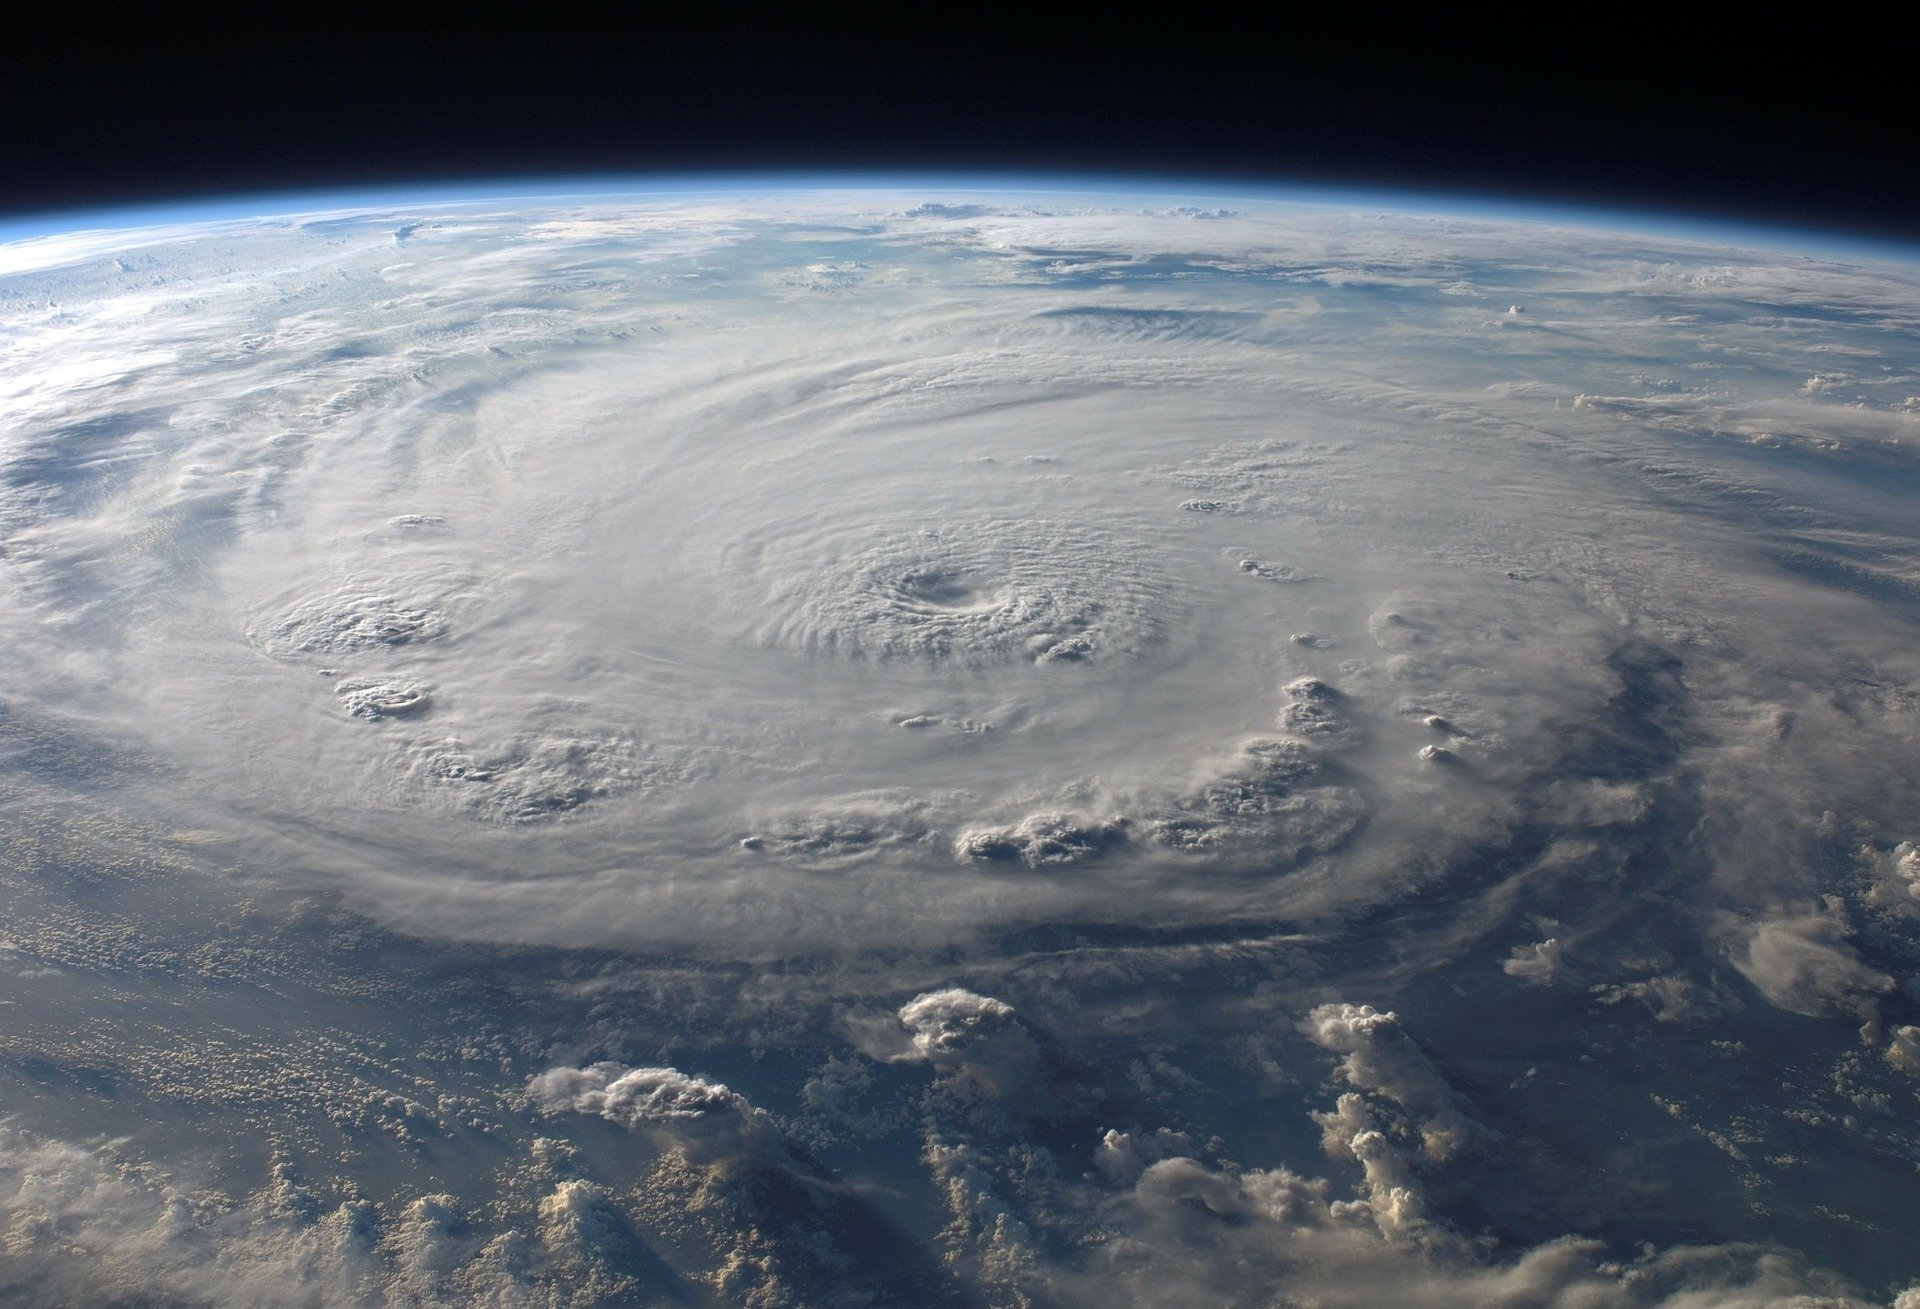
\includegraphics[width=\textwidth]{hurricane}\end{center}

What does the future hold?  Although we cannot peer forward and find out for sure, it turns out that in many cases we can use mathematical models to make predictions.  For instance, by tracking the development and path of a hurricane, we can predict where it will go next, although weather prediction is such a difficult problem that the true path is often very different from the prediction.  While we won't be tackling anything nearly as complicated as weather forecasting, we will see in this chapter how to build a few different types of mathematical models and use them to make predictions.

Of course, it is crucial to understand that no mathematical model is perfect.  There will always be a trade-off between the accuracy of a model and its simplicity.  The simpler a model, the more easily we can make predictions with it, but there will be more error in the approximation.  On the other hand, more precise models may be more difficult---or even impossible---to solve.  You should always remember, though, that every model is at best an imperfect representation of the real world, and there will always be some inherent error between what the model predicts and what actually occurs.
\vfill
\pagebreak

\section{Linear Models}
\setcounter{ExampleCounter}{1}
%\marginnote{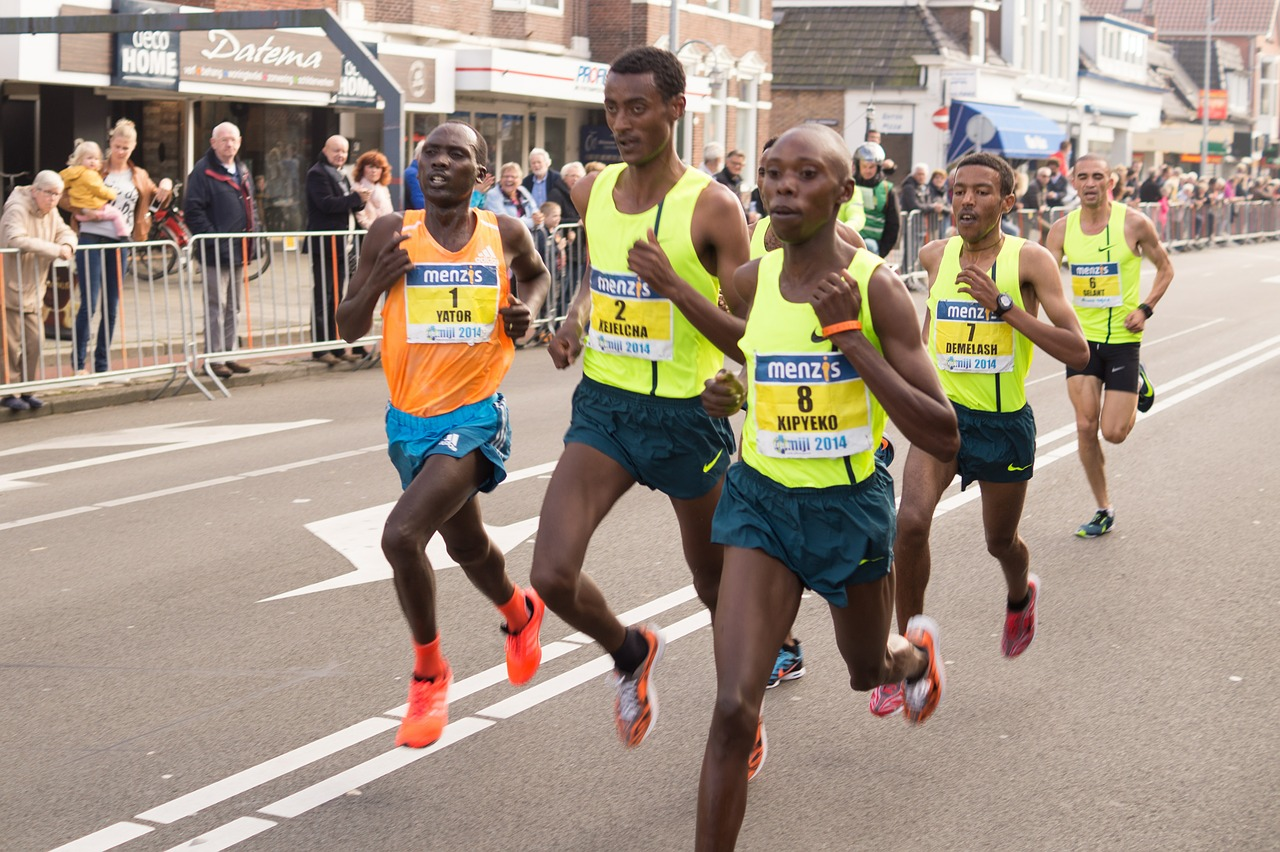
\includegraphics[scale=0.07]{Marathon1}}
If you decide to train for a marathon and you currently run 3 miles a day, you may choose to increase your distance by half a mile every week.  Can we predict how far you'll be running in six weeks, or how long it will take to reach your goal?  With small numbers like these, you could answer those questions without using an equation, but we'll use this as an example to show how to build a simple model from a scenario like this.

\begin{center}
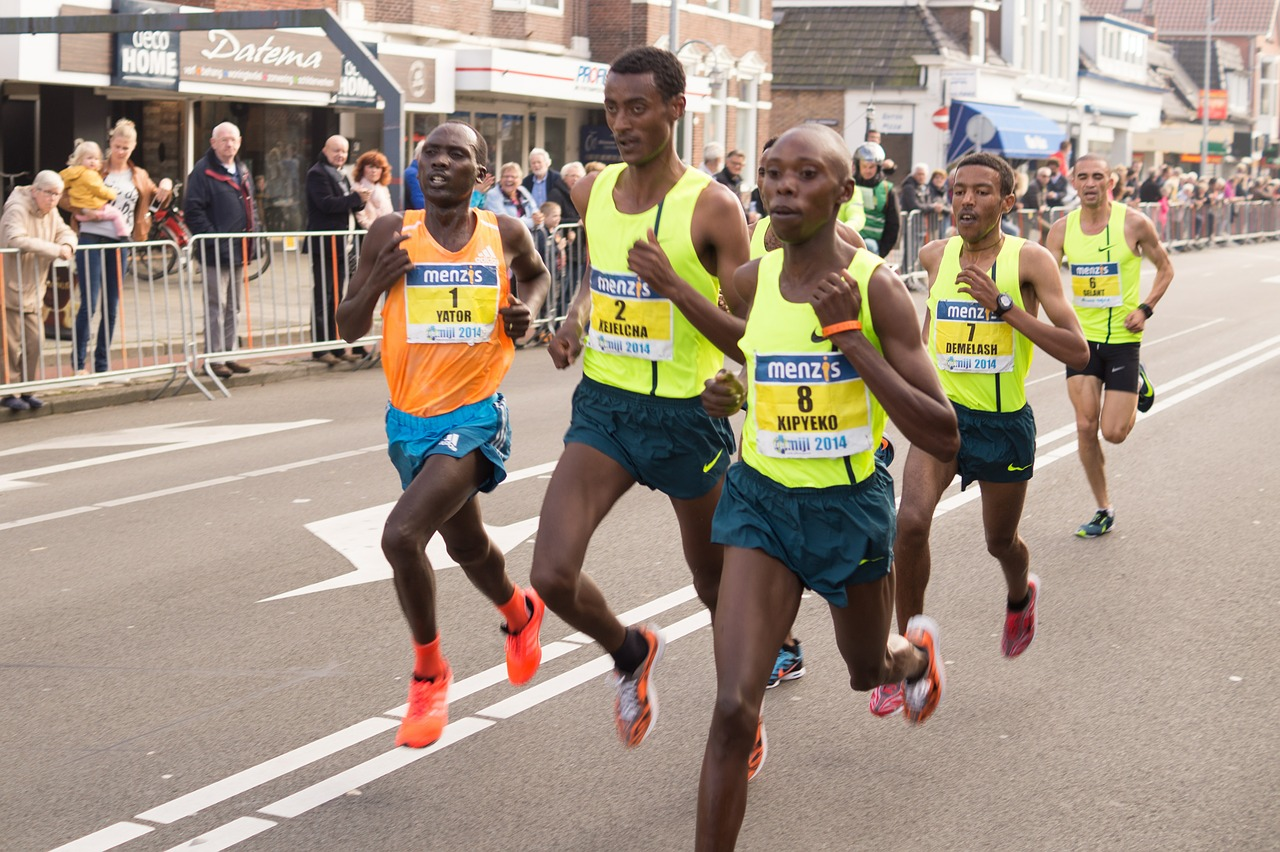
\includegraphics[width=0.8\textwidth]{Marathon1}
\end{center}

Let $P_t$ represent the number of miles that you run after $t$ weeks, so $P_0$ would be the number of miles you currently run, $P_1$ would represent the number of miles you run after 1 week, and so on.  We can define a \textbf{recursive relationship} like the following one to represent the scenario that was laid out.
\begin{align*}
P_0 &= 3\\
P_t &= P_{t-1} + 0.5
\end{align*}

A recursive relationship is one that defines each value in a sequence using previous values.  We could use this relationship to go from $P_0$ to $P_1$ to $P_2$ and so on, all the way to $P_6$ to answer the first question, and we could keep going from one value to the next until we reached 26 to answer the second question.  However, this would be tedious and mindless, so instead we prefer an \textbf{explicit equation}, or closed-form equation.  Especially for predictions far into the future, the recursive form is impractical, even though it arises easily from the problem description.

In this case, the explicit form is pretty straightforward, but deriving it from the recursive form will be instructive:
\begin{align*}
P_0 &= 3\\
P_1 &= 3+0.5\\
P_2 &= 3+0.5+0.5 = 3+(0.5)2\\
P_3 &= 3+0.5+0.5+0.5 = 3 + (0.5)3\\
&\vdots\\
P_t &= 3 + 0.5t
\end{align*}

This explicit equation gives an easy way to quickly answer both questions.  We can substitute 6 for $t$ to find that $P_6 = 3+0.5(6) = 6$ miles, and we can substitute 26 for $P_t$ and solve for $t$ to find how long it'll take to reach your goal:
\begin{align*}
26 &= 3+0.5t\\
23 &= 0.5t\\
46 &= t
\end{align*}
It'll take 46 weeks to reach your goal.
\begin{center}
\begin{tikzpicture}
\begin{axis}[
    xmin=0, xmax=47,
    ymin=0, ymax=30,
    axis lines=center,
    axis on top=false,
    domain=0:1,
    x=0.15cm,
    y=0.15cm,
    xtick={5,10,...,45},
    xticklabels={5,10,...,45},
    ytick={0,5,...,25},
    yticklabels={0,5,10,15,20,25,30},
    axis lines=middle,
    axis line style={->},
    x label style={at={(axis description cs:0.5,-0.1)},anchor=north},
    y label style={at={(axis description cs:-0.1,.5)},rotate=90,anchor=south},
    xlabel={Week},
    ylabel={Number of Miles},
    grid=major
    ]
	\addplot [blue,only marks,mark size=1] table {
	0 3
	1 3.5
	2 4
	3 4.5
	4 5
	5 5.5
	6 6
	7 6.5
	8 7
	9 7.5
	10 8
	11 8.5 
	12 9
	13 9.5
	14 10
	15 10.5
	16 11
	17 11.5
	18 12
	19 12.5
	20 13
	21 13.5
	22 14
	23 14.5
	24 15
	25 15.5
	26 16
	27 16.5
	28 17
	29 17.5
	30 18
	31 18.5
	32 19
	33 19.5
	34 20
	35 20.5
	36 21
	37 21.5
	38 22
	39 22.5
	40 23
	41 23.5
	42 24
	43 24.5
	44 25
	45 25.5
	46 26
	};
	%\addplot [blue, thick] table {
	
	%};
\end{axis}
\end{tikzpicture}
\end{center}

This graph shows why we call this \textit{linear} growth.  If we graph the number of miles versus the week, the points lie along a straight line.  This is consistent for every problem where a number grows by a constant amount every time period.  That's the key to linear growth: there's a constant growth amount, which we'll call $d$ (for \emph{difference}), that is added at each step.  For instance, in the marathon example, $d=0.5$ because half a mile is added each week.  Knowing that, the following formula should look familiar, because it is the same form that we developed above.

\begin{formula}{Linear Growth}
If some quantity starts at size $P_0$ and grows by $d$ every time period, then the quantity after $t$ time periods can be predicted using the following formula.

{\Large \[P_t = P_0 + dt\]}

Here $d$ represents the common difference---the amount that the quantity changes each time $t$ increases by 1.\\

Notice that this could refer to linear growth or linear decay; if $d$ is negative, the quantity will decrease linearly.
\end{formula}

Knowing that the key to linear growth is this common difference between terms, we can recognize linear growth from data if each term is the previous term plus a constant.
\begin{center}
\begin{tabular}{p{0.5in} p{0.75in} p{1.25in}}
\textbf{Term} & \textbf{Quantity} & \textbf{Difference from Previous Term}\\
\hline
& & \\
0 & 15 & \\
1 & 27 & 12\\
2 & 39 & 12\\
3 & 51 & 12\\
4 & 63 & 12\\
5 & 75 & 12\\
\end{tabular}
\end{center}
As we can observe in this table, if we note that the quantity adds a constant amount each time, we know that the growth is linear, and we can write the closed-form equation given above.\\

Notice that this is exactly the standard linear equation that you've seen in your algebra classes:
\begin{align*}
y &= mx+b\\
P_t &= dt + P_0
\end{align*}
Here, $P_0$ is the $y$-intercept, since it is the starting point, and thus the value when $t=0$.  Also, $d$ is the slope here, or the amount by which the quantity changes when $t$ increases by 1.

These two equations are the same, but as you'll see when modeling, we often rename the pieces to more closely match the names of the real-world quantities we're measuring.
\pagebreak

\begin{example}[https://www.youtube.com/watch?v=cpaNK4jbMkA&list=PLfmpjsIzhztutjEb8Pg5OBOlI1p80yVoy&index=1]{Elk Population}
The population of elk in a national forest was measured to be 12,000 in 2011 and 15,000 in 2015.  If the population continues to grow linearly at this rate, what do we expect the elk population to be in 2022?

\solline
\marginnote{\includegraphics[scale=0.07]{Elk1}}
We first need to define the parts of our linear growth equation.  The initial amount $P_0$ is the amount when $t=0$, but we won't use the actual year 0 as our starting point.  Instead, the initial amount in this problem is given in 2011, so we'll define $t=0$ to be the year 2011, so $P_0=12,000$.\\

Next we need to find $d$, the growth per time period.  Since the time period in this example is one year, we'll need to find how much the population grew each year.
\begin{center}
\begin{tabular}{c c}
\textbf{Year} & \textbf{Population}\\
\hline
0 & 12,000\\
4 & 15,000
\end{tabular}
\end{center}
Since the population grew by 3,000 in 4 years, this represents a growth of 3,000/4 = 750 per year.  Thus $d=750$.\\

Note that this is equivalent to using the slope formula: $\dfrac{\textrm{rise}}{\textrm{run}}$
\begin{align*}
d &= \textrm{ slope }\\
&= \dfrac{\textrm{change in population}}{\textrm{change in time}}\\
&= \dfrac{15,000 - 12,000}{2015 - 2011}\\
&= \dfrac{3000}{4}\\
&= 750
\end{align*}

Now we can write the explicit equation that models this population growth:
\[P_t = 12,000 + 750t\]

To answer the question, we note that 2022 corresponds to $t=11$, since 2022 is 11 years after 2011.
\begin{align*}
P_{11} &= 12,000 + 750(11)\\
&= \boxed{20,250 \textrm{ elk}}
\end{align*}
\end{example}

\begin{try}[http://hartleymath.com/versatilemath/tryit/\#/growth-models--linear-growth-model-(trout-population)]
If we estimated the population of trout in a pond to be 2200 in 2008 and 3500 in 2012, construct a linear model to predict the population in 2017.
\end{try}

Notice the key to that last problem: by knowing the population at the beginning and at the end, we can how much the population changes in a single year by dividing the total change by the number of years that elapsed.

In the next example, we'll look at data that is nearly linear, but not exactly.  However, for the purposes of making predictions, we'll treat it as if it follows a linear trend (remember, in the real world, data is messy).  We'll do exactly the same thing we just did in the previous example; we'll simply focus on the amount at the beginning and at the end, and divide the total growth by the amount of time that passed.
\vfill
\pagebreak

\begin{example}[https://www.youtube.com/watch?v=QoOdfeLBN0o&list=PLfmpjsIzhztutjEb8Pg5OBOlI1p80yVoy&index=2]{Gasoline Consumption}
Gasoline consumption in the US has been increasing steadily.  Data from 1995 to 2004 is shown below.  Find a linear model for this data, and use it to predict consumption in 2018.  If the trend continues, when will consumption reach 200 billion gallons?

\solline
\marginnote{\includegraphics[scale=0.16]{GasTanker1}}
\begin{center}
\begin{tabular}{|p{1in} | c | c | c | c | c | c | c | c | c | c|}
\hline
\textbf{Year} & '95 & '96 & '97 & '98 & '99 & '00 & '01 & '02 & '03 & '04\\
\hline
\parbox{0.9in}{\textbf{Consumption (billions}\\ \textbf{of gallons)}} & 116 & 118 & 119 & 123 & 125 & 126 & 128 & 131 & 133 & 136\\
\hline
\end{tabular}
\end{center}

If we plot this data, it appears to have an approximately linear relationship.
\begin{center}
\begin{tikzpicture}
\begin{axis}[
    xmin=0, xmax=12,
    ymin=0, ymax=25,
    axis lines=center,
    axis on top=false,
    domain=0:1,
    x=0.75cm,
    y=0.15cm,
    xtick={0,1,...,12},
    xticklabels={1994,1995,1996,1997,1998,1999,2000,2001,2002,2003,2004,2005},
    ytick={0,5,...,25},
    yticklabels={115,120,125,130,135,140},
    axis lines=middle,
    axis line style={->},
    x label style={at={(axis description cs:0.5,-0.1)},anchor=north},
    y label style={at={(axis description cs:-0.1,.5)},rotate=90,anchor=south},
    xlabel={Year},
    ylabel={Gas Consumption},
    grid=major
    ]
	\addplot [blue,only marks] table {
	1 1
	2 3
	3 4
	4 8
	5 10
	6 11
	7 13
	8 16
	9 18
	10 21
	};
	%\addplot [blue, thick] table {
	
	%};
\end{axis}
\end{tikzpicture}
\end{center}

One way to find a linear trend for data like this is a statistical technique known as \textit{linear regression}.  We will see examples of how to use the calculator for regression later in this section, and the chapter on Statistics will describe linear regression in more detail.

For now, though, we'll simply use the data from the first and last years to find the average growth each year (the slope of the line).\marginnote{We could use the data from any two years to calculate the slope (and we would get slightly different answers), but a common convention is to use the first and last years.  You should follow this convention when answering the homework questions.}
\begin{center}
\begin{tabular}{c | c}
\textbf{Year} & \textbf{Consumption}\\
\hline
1995 & 116\\
2004 & 136
\end{tabular}
\end{center}

\begin{align*}
d &= \textrm{ slope } = \dfrac{\textrm{change in consumption}}{\textrm{change in time}} = \dfrac{136 - 116}{2004 - 1995} = \dfrac{20}{9}\\
&= 2.22 \textrm{ billion gallons per year}
\end{align*}

Now we can write our model (in billions of gallons):
\[\boxed{P_t = 116 + 2.2t}\]
\begin{center}
\begin{tikzpicture}
\begin{axis}[
    xmin=0, xmax=12,
    ymin=0, ymax=25,
    axis lines=center,
    axis on top=false,
    domain=0:1,
    x=0.75cm,
    y=0.15cm,
    xtick={0,1,...,12},
    xticklabels={1994,1995,1996,1997,1998,1999,2000,2001,2002,2003,2004,2005},
    ytick={0,5,...,25},
    yticklabels={115,120,125,130,135,140},
    axis lines=middle,
    axis line style={->},
    x label style={at={(axis description cs:0.5,-0.1)},anchor=north},
    y label style={at={(axis description cs:-0.1,.5)},rotate=90,anchor=south},
    xlabel={Year},
    ylabel={Gas Consumption},
    grid=major
    ]
	\addplot [blue,only marks] table {
	1 1
	2 3
	3 4
	4 8
	5 10
	6 11
	7 13
	8 16
	9 18
	10 21
	};
	\addplot [blue, thick,dashed,domain=1:10] {2.2*x-1};
\end{axis}
\end{tikzpicture}
\end{center}
\vfill
\pagebreak

We can use our model to make predictions about the future, using the simplifying assumption that the previous trend continues unchanged.
\begin{itemize}
\item Predicting gas consumption in 2018, when $t=23$:\marginnote{This example illustrates the two main types of questions that we often want to answer:\\ \text{}\\
1. Predicting the value of what we are measuring at a given point in time.\\ \text{}\\
2. Predicting the point in time when the thing we are measuring will reach a certain value.}
\[P_{23} = 116 + 2.2(23) = \boxed{166.6}\]
Our model predicts that the US will consume 166.6 billion gallons of gasoline in 2018 if the current trend continues.

\item Predicting when consumption reaches 200 billion gallons:
\begin{align*}
200 &= 116 + 2.2t\\
84 &= 2.2t\\
\boxed{38.18} &= t
\end{align*}
This model predicts that gas consumption will reach 200 billion gallons about 38 years after 1995, or the year 2033.
\end{itemize}
\end{example}

\begin{try}[http://hartleymath.com/versatilemath/tryit/\#/growth-models--stay-at-home-fathers]
The number of stay-at-home fathers in Canada has been growing steadily at an approximately linear rate.  Use the data from the table below to find an explicit formula for the number of stay-at-home fathers and use it to predict the number in 2020.  Use 1976 and 2010 to find the average rate of change.
\begin{center}
\begin{tabular}{|p{1.25in} | c | c | c | c | c|}
\hline
\textbf{Year} & 1976 & 1984 & 1991 & 2000 & 2010\\
\hline
\textbf{Number of stay-at-home fathers} & 20,610 & 28,725 & 43,530 & 47,665 & 53,555\\
\hline
\end{tabular}
\end{center}
\end{try}

Again, we understand that this model is not perfect; the US will most likely not consume exactly 166.6 billion gallons of gas in 2018, but we expect consumption to be \textit{about} that.  In practice, we'll often make predictions and then compare them to actual measured results to assess the accuracy of our model.  A very simple linear model like this will likely have fairly large error; more sophisticated models tend to have smaller errors.

\subsection{Predicting Time}
As we pointed out in the previous example, there are generally two questions that we'll encounter with mathematical models like the ones in this chapter:
\begin{itemize}
\item At a given time, find the amount
\item For a given amount, find the time it will take to reach that level
\end{itemize}

The first question is generally easier, simply because of how the formula is arranged:
\[P_t = P_0 + dt\]
Since we know everything on the right-hand side of the equation in this case, we can plug it all in and simply carry out the arithmetic; what we want to know is already isolated on the left side.

It's slightly more tricky to solve for $t$ in the second question, because it requires some algebra to rearrange the pieces of the formula so that $t$ will be isolated on one side.  This gets even more difficult for more complicated models, like the ones in the rest of the chapter, because the algebraic steps are more involved.

\subsubsection*{Another option: use a calculator}
Although you should be able to carry out the algebraic steps, and it will likely be quicker to do so with linear models, let's see how to use the calculator to accomplish the same purpose.  What we're about to see will work no matter which part of the equation we want to solve for, so we will return to this method in each section in this chapter when we want to solve for $t$.
\vfill
\pagebreak

The key to this method involves graphing both sides of an equation and using the \texttt{intersect} option on a graphing calculator.  If you have a TI-83 or 84 or similar, you can look under the \texttt{CALC} menu, which you can find by pressing \calcbutton{2ND} and \calcbutton{TRACE}:
\begin{center}
\includegraphics[width=2in]{calculatorIntersect}
\end{center}

Before diving into the details, let's see why this works by going all the way back to the opening example of this section: the marathon training program.  Remember that we drew this graph to represent the number of miles that you would run each week:
\begin{center}
\begin{tikzpicture}
\begin{axis}[
    xmin=0, xmax=47,
    ymin=0, ymax=30,
    axis lines=center,
    axis on top=false,
    domain=0:1,
    x=0.15cm,
    y=0.15cm,
    xtick={5,10,...,45},
    xticklabels={5,10,...,45},
    ytick={0,5,...,25},
    yticklabels={0,5,10,15,20,25,30},
    axis lines=middle,
    axis line style={->},
    x label style={at={(axis description cs:0.5,-0.1)},anchor=north},
    y label style={at={(axis description cs:-0.1,.5)},rotate=90,anchor=south},
    xlabel={Week},
    ylabel={Number of Miles},
    grid=major
    ]
	\addplot [blue,only marks,mark size=1] table {
	0 3
	1 3.5
	2 4
	3 4.5
	4 5
	5 5.5
	6 6
	7 6.5
	8 7
	9 7.5
	10 8
	11 8.5 
	12 9
	13 9.5
	14 10
	15 10.5
	16 11
	17 11.5
	18 12
	19 12.5
	20 13
	21 13.5
	22 14
	23 14.5
	24 15
	25 15.5
	26 16
	27 16.5
	28 17
	29 17.5
	30 18
	31 18.5
	32 19
	33 19.5
	34 20
	35 20.5
	36 21
	37 21.5
	38 22
	39 22.5
	40 23
	41 23.5
	42 24
	43 24.5
	44 25
	45 25.5
	46 26
	};
	%\addplot [blue, thick] table {
	
	%};
\end{axis}
\end{tikzpicture}
\end{center}

Now, let's ask this question: how long will it take to reach the goal of running 26 miles?  Notice that what this means on the graph is: when does that blue line reach a height of 26?  If we draw a horizontal line at 26, we can zero in on the point where the two lines cross (or intersect) and trace downward to the $x$-axis to find the time when that intersection occurs.

\begin{center}
\begin{tikzpicture}
\begin{axis}[
    xmin=0, xmax=50,
    ymin=0, ymax=30,
    axis lines=center,
    axis on top=false,
    domain=0:1,
    x=0.15cm,
    y=0.15cm,
    xtick={5,10,...,50},
    xticklabels={5,10,...,50},
    ytick={0,5,...,25},
    yticklabels={0,5,10,15,20,25,30},
    axis lines=middle,
    axis line style={->},
    x label style={at={(axis description cs:0.5,-0.1)},anchor=north},
    y label style={at={(axis description cs:-0.1,.5)},rotate=90,anchor=south},
    xlabel={Week},
    ylabel={Number of Miles},
    grid=major
    ]
	\addplot [blue, thick,domain=0:50] {0.5*x+3};
	\addplot [blue, thick,dashed,domain=0:50] {26};
	\draw [red, thick, dashed] (axis cs:46,0) -- (axis cs:46,30);
	\draw [red, ultra thick] (axis cs:46,26) circle (10);
\end{axis}
\end{tikzpicture}
\end{center}

In other words, when we find the coordinates of the intersection point, the $y$-coordinate will be the level we're given to predict the time for, and the $x$-coordinate will be the time at which that level is reached.\\

On the calculator, this means we have to graph two functions: one will be the model that we have built ($P_t = P_0 + dt$ for linear models in this section, other formulas for later sections), and the other will be a constant value, whatever value we want to know the corresponding time for.  Once we find the intersection, the $x$-coordinate will be the time value that we're looking for.

To illustrate how to use this method, we'll continue to use the same example: remember that the model we built was $P_t = 3 + 0.5t$, and we wanted to predict when the number of miles would reach 26.  Thus, we need to graph $y_1=3+0.5x$ and $y_2=26$ on the calculator; note that the calculator always uses $x$ and $y$ instead of $t$ and $P_t$.
\vfill
\pagebreak

\subsubsection*{Step 1: graph both functions}
To begin, press the \calcbutton{Y=} button in the upper-left corner to open the graphing menu, then enter the two functions as $Y_1$ and $Y_2$.  Note that to enter $X$, use the button labeled $\boxed{X, T, \theta, n}$
\begin{center}
\includegraphics[width=2in]{calculatorIntersectEx1}
\end{center}

\subsubsection*{Step 2: zoom to see the intersection}
When you press \calcbutton{GRAPH} you may see something like this:
\begin{center}
\includegraphics[width=2in]{calculatorIntersectEx2}
\end{center}

Only one line is visible, because the window is too zoomed in to see the other.  To zoom out, you can press the \calcbutton{ZOOM} button and select one of the options, like \texttt{3. Zoom Out}.  If you press the \calcbutton{WINDOW} button, though, you can manually set the boundaries of the window, and if you have a sense of roughly where the intersection should occur, that's usually the easiest way to adjust the view so that you can see both lines.

In this case, we know that the upper end of the window needs to go up to at least 26, since that is the $y$-coordinate of the intersection, so let's use 30 as the upper limit.  With a bit of trial and error, we can find a reasonable upper limit on $x$ as well; we'll use 50 for this one.
\begin{center}
\includegraphics[width=2in]{calculatorIntersectEx3}
\end{center}

If you press \calcbutton{GRAPH} again, you should see this:
\begin{center}
\includegraphics[width=2in]{calculatorIntersectEx4}
\end{center}

We can now see the intersection point on the graph, but we have a bit more work to do to find its coordinates.
\pagebreak

\subsubsection*{Step 3: find the intersection}
Now if you press \calcbutton{2ND} and \calcbutton{TRACE} to open the \texttt{CALC} menu and select the option labeled \texttt{5. intersect}, you'll see something like this:
\begin{center}
\includegraphics[width=2in]{calculatorIntersectEx5}
\end{center}

What's happening here?  Without getting too specific, the way the calculator finds the intersection point involves starting with an initial guess, and then searching nearby in both directions to find the crossing point.  This means it will ask where you want to start looking on the first curve, where you want to start looking on the second curve, and where your overall initial guess is.  You can use the arrow keys to move the blinking cursor closer to the intersection if you like, but for simple examples like the ones in this chapter, the calculator will find it even if we don't feed it a starting point that is close by.

In practice, this means that if you like, you can simple press \calcbutton{ENTER} three times to accept the default starting values.

Once you do this, you should see the following:
\begin{center}
\includegraphics[width=2in]{calculatorIntersectEx6}
\end{center}

At the bottom of the screen, you can see the coordinates of the intersection point.  Notice that the $y$-coordinate is no surprise; that's based on the given number of miles that we were trying to reach.  The $x$-coordinate is the answer we were looking for, the value of $t$ when we reach 26 miles.

\subsection{Linear Regression Using the Calculator}
Usually when we build a model, we do so using data from the past to predict the future.  In most of the examples in this section, we drew a straight line by selecting the first and last points and finding the slope that connected them.

There is another approach, using a statistical technique known as \textbf{linear regression}.  We will omit the details here, but a more thorough discussion can be found in the Statistics chapter.  For our purposes, we will simply see how to use a graphing calculator to find the equation of a line that most closely fits the data we're given.

Rather than simply using two points, linear regression takes all of the data points into account and builds a \textit{line of best fit}; the principles needed to describe how this best-fit process works require some statistics knowledge, so we will not discuss it further in this chapter.\\

We'll use the gasoline consumption example to show how to use the calculator for this.  Recall that we were given the following data (and the resulting graph):
\begin{center}
\begin{tabular}{|p{1in} | c | c | c | c | c | c | c | c | c | c|}
\hline
\textbf{Year} & '95 & '96 & '97 & '98 & '99 & '00 & '01 & '02 & '03 & '04\\
\hline
\parbox{0.9in}{\textbf{Consumption (billions}\\ \textbf{of gallons)}} & 116 & 118 & 119 & 123 & 125 & 126 & 128 & 131 & 133 & 136\\
\hline
\end{tabular}
\end{center}

\begin{center}
\begin{tikzpicture}
\begin{axis}[
    xmin=0, xmax=12,
    ymin=0, ymax=25,
    axis lines=center,
    axis on top=false,
    domain=0:1,
    x=0.75cm,
    y=0.15cm,
    xtick={0,1,...,12},
    xticklabels={1994,1995,1996,1997,1998,1999,2000,2001,2002,2003,2004,2005},
    ytick={0,5,...,25},
    yticklabels={115,120,125,130,135,140},
    axis lines=middle,
    axis line style={->},
    x label style={at={(axis description cs:0.5,-0.1)},anchor=north},
    y label style={at={(axis description cs:-0.1,.5)},rotate=90,anchor=south},
    xlabel={Year},
    ylabel={Gas Consumption},
    grid=major
    ]
	\addplot [blue,only marks] table {
	1 1
	2 3
	3 4
	4 8
	5 10
	6 11
	7 13
	8 16
	9 18
	10 21
	};
	%\addplot [blue, thick] table {
	
	%};
\end{axis}
\end{tikzpicture}
\end{center}

The model we built in that example was $P_t = 116 + 2.2t$; we'll keep this handy to compare it to the answer we get using regression.

\subsubsection*{Step 1: enter the data}
First, we need to enter the data that we're given (in full).  To do this, press the \calcbutton{STAT} button; the first menu that you will see should look like this:
\begin{center}
\includegraphics[width=2in]{gmRegression1}
\end{center}

Simply press \calcbutton{ENTER} to enter the \texttt{Edit} menu, where we can enter the data; first, you should see the following (if there is data already there, simply use the arrow keys to move up to the label of one of the lists, and press \calcbutton{CLEAR}):

\begin{center}
\includegraphics[width=2in]{gmRegression2}
\end{center}

In list \texttt{L1}, enter the values for $t$.  Notice that here we set 1995 as the initial year, or year 0, so start with 0 and enter enough values to get to 2004 (year 9).  In list \texttt{L2}, enter the values for gasoline consumption.

\begin{center}
\includegraphics[width=2in]{gmRegression3}
\end{center}
\pagebreak

\subsubsection*{Step 2: calculate the regression equation}

Now, to calculate the regression equation, press the \calcbutton{STAT} button again, and use the right arrow key to move to the \texttt{CALC} menu.  There are many options here, but the one we want at the moment is \texttt{4: LinReg(ax+b)}.  Notice that this means that we'll receive answers for \texttt{a} and \texttt{b}, and these will represent the slope and intercept, respectively.

\begin{center}
\includegraphics[width=2in]{gmRegression4}
\end{center}

If you select the linear regression option, you should see the following menu:

\begin{center}
\includegraphics[width=2in]{gmRegression5}
\end{center}

Since we entered the time values in \texttt{L1} and the consumption values in \texttt{L2}, we don't need to change anything here, so simply scroll down to select \texttt{Calculate} and press \calcbutton{ENTER}\ , which shows the results:

\begin{center}
\includegraphics[width=2in]{gmRegression6}
\end{center}

For now, all we're interested in is the values of \texttt{a} and \texttt{b}; to put it in more familiar terms, the equation of the regression model is
\[P_t = 115.7 + 2.19t\]

Compare this to the one we built by hand.  Since this data was fairly linear, there isn't much difference between the two answers; if there were \emph{outliers} (unusual values that deviate significantly from the linear trend), there might be a greater difference.

In general, the manual method is easier and quicker to do, but this statistical method gives more accurate results.
\pagebreak

\subsection{Using Excel}
We can also use Excel to calculate regression equations.  To begin, enter the data as shown (we're using the same example as we did with the calculator, for comparison):

\begin{center}
\includegraphics[width=0.6\textwidth]{gmRegressionExcel1}
\end{center}

Next, we need to insert a scatterplot of these data points; select the Insert menu at the top of the screen, then select the scatterplot option under the Charts section (select the first type of scatterplot under that submenu).

\begin{center}
\includegraphics[width=0.6\textwidth]{gmRegressionExcel2}
\end{center}

This creates a graph similar to the one that we drew earlier for this same example; we could add a title to the chart and the axes, but we won't bother for this example.

\begin{center}
\includegraphics[width=0.6\textwidth]{gmRegressionExcel3}
\end{center}

To add a regression line, click on the plus symbol at the upper right (when the chart is selected).  One of the options is to add a trendline.  If you check that box, the line will be drawn, but by default, Excel won't show the equation of the line, which is what we're after, so we need to select ``More Options'' after clicking on the arrow next to the trendline option.

\begin{center}
\includegraphics[width=0.6\textwidth]{gmRegressionExcel4}
\end{center}

This brings up the following menu.  Notice that there are different types of equations we can use to model the data, including several that we'll encounter later in the chapter.  For now, though, leave the linear option selected, but check the box at the bottom of the menu that says ``Display Equation on chart.''

\begin{center}
\includegraphics[width=0.6\textwidth]{gmRegressionExcel5}
\end{center}

This leads to the following:

\begin{center}
\includegraphics[width=0.6\textwidth]{gmRegressionExcel6}
\end{center}

The equation, as calculated by Excel, is \[P_t = 115.65 + 2.1879t\] which, after rounding, is identical to the one obtained by the calculator (this is no surprise, since they're using the same formulas).

\subsection{When Good Models Go Bad}
When predicting the future with mathematical models, it is crucial to keep in mind that few trends continue indefinitely.

\begin{example}[https://www.youtube.com/watch?v=7_wAlvsCyDc&list=PLfmpjsIzhztutjEb8Pg5OBOlI1p80yVoy&index=3]{A Boy's Height}
Suppose a four year old boy is currently 39 inches tall, and you are told to expect him to grow 2.5 inches a year.\\

We can set up a growth model, with $t=0$ corresponding to 4 years old.
\[P_t = 39 + 2.5t\]

At six years old (when $t=2$), we would expect him to be
\[P_2 = 44 \textrm{ inches tall},\]
but this model eventually breaks down.  Certainly, we shouldn't expect him to grow at the same rate all his life.  If he did, at age 50 he would be
\[P_{46} = 154 \textrm{ inches } = 12.8 \textrm{ feet tall}.\]
\end{example}

Of course, this boy will not grow at a constant rate, but rather experience growth spurts and ultimately stop growing in his early 20s.  But this example also illustrates that we should check our model against common sense.
\vspace{0.5in}

Let's look at another example that illustrates the need for a common sense check.

\begin{example}[https://www.youtube.com/watch?v=3FeV7lvkATI&list=PLfmpjsIzhztutjEb8Pg5OBOlI1p80yVoy&index=4]{Marathon Times}
The table and graph below show the record times for the marathon for men and women from 1965 to 1980.
\begin{center}\marginnote{\includegraphics[scale=0.07]{WomanRunner1}}
\begin{tabular}{l | c | c}
\textbf{Year} & \textbf{\color{blue}Men's Times (min)} & \textbf{\color{orange!70!black}Women's Times (min)}\\
\hline
& & \\
1965 & 132 & \\
1966 & & \\
1967 & 129.5 & 195\\
1968 & & \\
1969 & 128.5 & \\
1970 & 129.5 & 183\\
1971 & & 175\\
1972 & & \\
1973 & & 166\\
1974 & 129 & 163\\
1975 & & 158\\
1976 & & \\
1977 & & 155\\
1978 & 129 & 152\\
1979 & & 147\\
1980 & 129 & 145\\
\end{tabular}
\end{center}

\begin{center}
\begin{tikzpicture}
\begin{axis}[
    xmin=0, xmax=18,
    ymin=0, ymax=80,
    axis lines=center,
    axis on top=false,
    domain=0:1,
    x=0.45cm,
    y=0.055cm,
    xtick={0,2,...,18},
    xticklabels={1964,1966,1968,1970,1972,1974,1976,1978,1980,1982},
    ytick={0,10,...,80},
    yticklabels={120,130,140,150,160,170,180,190,200},
    axis lines=middle,
    axis line style={->},
    x label style={at={(axis description cs:0.5,-0.1)},anchor=north},
    y label style={at={(axis description cs:-0.1,.5)},rotate=90,anchor=south},
    xlabel={Year},
    ylabel={Marathon Time in Minutes},
    grid=major
    ]
	\addplot [blue,only marks] table {
	1 12
	3 9.5
	5 8.5
	6 9.5
	10 9
	14 9
	16 9
	};
	\addplot [orange!70!black,only marks] table {
	3 75
	6 63
	7 55
	9 46
	10 43
	11 38
	13 35
	14 32
	15 27
	16 25
	};
\end{axis}
\end{tikzpicture}
\end{center}

From this data, it looks like both sets of data are following a linear trend.  If we use the first and last data points to find the average rate of change for each, we get the following linear models, using 1967 as $t=0$:
\begin{align*}
M_t &= 129.5-0.2t\\
W_t &= 195-3.85t
\end{align*}

According to these two linear models, we would predict that the women's record would beat the men's record by 1985; however, in 1985, the men's record was still 14 minutes faster than the women's.  What happened here?\\

Since women began setting marathon records about 50 years later than men, in the early years their progress was drastic, but eventually slowed down, and the trend was not linear over the long run (wow, what a terrible pun).
\end{example}

It should be clear that this linear trend was misleading, since if we extrapolated this model too far forward, we'd get ridiculous results.  The model predicts, for instance, that women would run the marathon in 1:20:00 in 1997 (a pace of about 20 mph, the speed of a roadrunner or close to the top speed of Usain Bolt at full sprint), or that by 2017 they'd be running it in 2.5 minutes (around 630 mph).

The lesson is simple, and hopefully obvious: linear trends are usually only useful in the short term; few phenomena follow linear trends over the long term.  That is why we'll examine other types of models in the coming sections.  However, keep this in mind, because we'll find that even those more sophisticated models have their limitations, and often they too break down in the long term.
\begin{exercises}
\ptwo{Marko currently has 20 tulips in his yard.  Each year he plants 5 more.
\begin{enumerate}[(a)]
\item Find a linear model of the form $P_t = P_0 + dt$ to describe the number of tulips Marko has at a given point in time.
\item How many tulips will Marko have in 7 years?
\item When will Marko have 65 tulips?
\end{enumerate}}
\ptwo{Pam is a DJ.  Every week she buys 3 new albums to add to her collection.  She currently owns 450 albums.
\begin{enumerate}[(a)]
\item Find a linear model of the form $P_t = P_0 + dt$ to describe the number of albums Pam has at a given point in time.
\item How many albums will Pam have in 11 weeks?
\item When will Pam have 489 albums?
\end{enumerate}}

\ptwo{A store did \$40,000 in sales in 2016, and \$62,000 in 2018.
\begin{enumerate}[(a)]
\item Assuming the store's sales are growing linearly, find the growth rate $d$.
\item Write a linear model to describe this store's sales from 2016 onward.
\item Predict the store's sales in 2025.
\item When do you expect the store's sales to exceed \$100,000?
\end{enumerate}}
\ptwo{A small town had 340 homes in 2010, and by 2020, this had grown to 375.
\begin{enumerate}[(a)]
\item Assuming the number of homes is growing linearly, find the growth rate $d$.
\item Write a linear model to describe the number of homes in this town from 2010 onward.
\item Predict how many homes there will be in this town in 2034.
\item When do you expect the number of homes to exceed 500?
\end{enumerate}}

\ptwo{A population of beetles is growing according to a linear growth model.  Initially, there were 13 beetles, and 8 weeks later, there were 42 beetles.
\begin{enumerate}[(a)]
\item Write a linear model to describe the number of beetles over time, using weeks as the unit of time.
\item How many beetles are there expected to be 14 weeks after the initial point?
\item When do you expect the number of beetles to exceed 70?
\end{enumerate}}
\ptwo{The number of streetlights in a town is growing linearly.  Four months ago there were 130 lights.  Now there are 146 lights.
\begin{enumerate}[(a)]
\item Write a linear model to describe the number of streetlights in the town over time, using months as the unit of time.
\item How many streetlights are expected a year from \emph{now} (not a year from the beginning)?
\item When do you expect the number of streetlights to exceed 200?
\end{enumerate}}

\ptwo{In 1990, there were 112 nuclear power plants in the U.S.  By 2019, this number had fallen to 96.
\begin{enumerate}[(a)]
\item Write a linear model to describe the number of nuclear power plants from 1990 onward.
\item Using this linear model, predict the number of nuclear power plants in the U.S. in 2030.
\item When do you expect the number of nuclear power plants to reach 80?
\end{enumerate}}
\ptwo{In 1990, approximately 1,820,000 violent crimes were reported in the U.S.  By 2019, this number had fallen to approximately 1,200,000.
\begin{enumerate}[(a)]
\item Write a linear model to describe the number of violent crimes in the U.S. from 1990 onward.
\item Using this linear model, predict the number of violent crimes in 2040.
\item When do you expect the number of violent crimes to reach 1,000,000?
\end{enumerate}}
\vfill
\pagebreak

\ptwo{The table below shows the average annual cost of health insurance for a single individual, from 1999 to 2019, according to the Kaiser Family Foundation.
\begin{center}
\begin{tabular}{c c}
\textbf{Year} & \textbf{Cost}\\
\hline
 & \\
1999 & \$2,196\\
2000 & \$2,471\\
2001 & \$2,689\\
2002 & \$3,083\\
2003 & \$3,383\\
2004 & \$3,695\\
2005 & \$4,024\\
2006 & \$4,242\\
2007 & \$4,479\\
2008 & \$4,704\\
2009 & \$4,824\\
2010 & \$5,049\\
2011 & \$5,429\\
2012 & \$5,615\\
2013 & \$5,884\\
2014 & \$6,025\\
2015 & \$6,251\\
2016 & \$6,435\\
2017 & \$6,690\\
2018 & \$6,896\\
2019 & \$7,186
\end{tabular}
\end{center}
\begin{enumerate}[(a)]
\item Using only the data from the first and last years, build a linear model to describe the cost of individual health insurance from 1999 onward.
\item Using this linear model, predict the cost of insurance in 2030.
\item According to this model, when do you expect the cost of individual insurance to reach \$12,000?
\item Using a calculator or spreadsheet program, build a linear regression model to describe the cost of individual insurance from 1999 onward.
\item Using the regression model, predict the cost of insurance in 2030.
\item According to the regression model, when do you expect the cost of individual insurance to reach \$12,000?
\end{enumerate}}
\ptwo{The table below shows the average annual cost of health insurance for a family, from 1999 to 2019, according to the Kaiser Family Foundation.
\begin{center}
\begin{tabular}{c c}
\textbf{Year} & \textbf{Cost}\\
\hline
 & \\
1999 & \$5,791\\
2000 & \$6,438\\
2001 & \$7,061\\
2002 & \$8,003\\
2003 & \$9,068\\
2004 & \$9,950\\
2005 & \$10,880\\
2006 & \$11,480\\
2007 & \$12,106\\
2008 & \$12,680\\
2009 & \$13,375\\
2010 & \$13,770\\
2011 & \$15,073\\
2012 & \$15,745\\
2013 & \$16,351\\
2014 & \$16,834\\
2015 & \$17,545\\
2016 & \$18,142\\
2017 & \$18,764\\
2018 & \$19,616\\
2019 & \$20,576
\end{tabular}
\end{center}
\begin{enumerate}[(a)]
\item Using only the data from the first and last years, build a linear model to describe the cost of family health insurance from 1999 onward.
\item Using this linear model, predict the cost of insurance in 2025.
\item According to this model, when do you expect the cost of family insurance to reach \$30,000?
\item Using a calculator or spreadsheet program, build a linear regression model to describe the cost of family insurance from 1999 onward.
\item Using the regression model, predict the cost of insurance in 2025.
\item According to the regression model, when do you expect the cost of family insurance to reach \$30,000?
\end{enumerate}}
\end{exercises}

\section{Quadratic Models}
\setcounter{ExampleCounter}{1}
In reality, straight lines are rare; this is as true with data as it is with stone formations.  Real data hardly ever follows such a simple rule, but whenever we can, we like to use lines to approximate real trends because straight lines are easy to work with.

\begin{center}
\includegraphics[width=0.8\textwidth]{StoneArch}
\end{center}

However, as we found at the end of the previous section, linear models will not work in every situation, and trying to force a linear trend on real data often leads to nonsensical results.  For the rest of this chapter, we'll study other models--using slightly more complicated formulas--that can be used when the data does not follow a linear trend.

Picking which model to use is a hard question, and this decision is usually based on looking at a graph and looking for a pattern, or trying multiple models and seeing which gives the best results.  That kind of decision is largely beyond the scope of this chapter; we'll focus on learning some basic features of a few different models, and the questions in each section will specify which kind of model to use.

We'll discuss three types of non-linear models:
\begin{enumerate}
\item Quadratic Models
\item Exponential Models
\item Logistic Models
\end{enumerate}

This section will focus on quadratic models, and the last two types will be the topics of the remaining sections in this chapter.

\subsection{Quadratic Models: Parabolas}
\marginnote{\includegraphics[width=1.5in]{WaterParabola}}
The next time you use a water fountain, watch the path that the water follows.  There's a certain elegance to this arch, and we have a special name for it: a \textbf{parabola}.  Every time a baseball player throws a ball, that ball's path follows this same pattern.  In fact, every time anything is launched or thrown, it follows a parabolic arch.

It turns out that this shape comes from a simple mathematical operation: \emph{squaring}.  Yes, that's it; when you square numbers, this pattern emerges.

Of course, that's not clear immediately, so let's do a simple experiment: square the whole numbers from 0 to 4, as well as the matching negative numbers.  We can arrange our results in a table like this:
\begin{center}
\begin{tabular}{c | c c c c c c c c c}
$x$ & $-4$ & $-3$ & $-2$ & $-1$ & 0 & 1 & 2 & 3 & 4\\
& & & & & & & & & \\
\hline
& & & & & & & & & \\
$x^2$ & 16 & 9 & 4 & 1 & 0 & 1 & 4 & 9 & 16
\end{tabular}
\end{center}

Notice the symmetry in the results: when we square 2 and $-2$, for instance, we get the same result, because multiplying two negative numbers results in a positive answer.  Look at the picture of the fountain in the margin; one of the main features of a parabola is its symmetry, and we're already starting to see that emerge.
\pagebreak

Just like we did in the previous section, let's graph these results and see what visual pattern we can observe.
\begin{center}
\begin{tikzpicture}
\begin{axis}[
    xmin=-4.5, xmax=4.5,
    ymin=-0.5, ymax=18,
    axis lines=center,
    axis on top=false,
    domain=0:1,
    x=0.6cm,
    y=0.3cm,
    xtick={-4,-3,...,4},
    xticklabels={-4,-3,...,4},
    ytick={0,2,...,18},
    yticklabels={0,2,...,18},
    axis lines=middle,
    axis line style={->},
    %x label style={at={(axis description cs:0.5,-0.1)},anchor=north},
    %y label style={at={(axis description cs:-0.1,.5)},rotate=90,anchor=south},
    xlabel={$x$},
    ylabel={$x^2$},
    grid=major
    ]
	\addplot [blue,only marks,mark size=2] table {
	-4 16
	-3 9
	-2 4
	-1 1
	0 0
	1 1
	2 4
	3 9
	4 16
	};
\end{axis}
\end{tikzpicture}
\end{center}

And if we connect the dots by filling in the results we would get if we applied this same rule to non-whole numbers, what do we get?

\begin{center}
\begin{tikzpicture}
\begin{axis}[
    xmin=-4.5, xmax=4.5,
    ymin=-0.5, ymax=18,
    axis lines=center,
    axis on top=false,
    domain=0:1,
    x=0.6cm,
    y=0.3cm,
    xtick={-4,-3,...,4},
    xticklabels={-4,-3,...,4},
    ytick={0,2,...,18},
    yticklabels={0,2,...,18},
    axis lines=middle,
    axis line style={->},
    %x label style={at={(axis description cs:0.5,-0.1)},anchor=north},
    %y label style={at={(axis description cs:-0.1,.5)},rotate=90,anchor=south},
    xlabel={$x$},
    ylabel={$x^2$},
    grid=major
    ]
	\addplot [blue,only marks,mark size=2] table {
	-4 16
	-3 9
	-2 4
	-1 1
	0 0
	1 1
	2 4
	3 9
	4 16
	};
	\addplot [blue, ultra thick, domain=-5:5] {x^2};
\end{axis}
\end{tikzpicture}
\end{center}

Look at that: we got exactly the same shape as the water rising and falling in the fountain (although flipped upside-down).  It's amazing what beauty can come from such a simple mathematical rule: when you start squaring numbers, you find a parabolic curve, and it turns out that this curve governs much of the motion we see around us every day.

Now, by comparing this graph with the picture of the fountain, we can observe that while parabolas all have the same structure, there are differences in the exact paths.  For instance, some of the jets in the fountain are aimed higher than others, leading to taller, narrower arches, while the lower jets create shorter, wider arches.  And the graph shows a parabola that is oriented in the opposite direction.

Where do these differences come from?  It's important to remember that the basic structure of the parabola is generated by squaring the inputs (we used $t$ in the previous section; these are the values for which we want to make predictions) to get $x^2$ (or $t^2$ if we use $t$ as the label for our variable).  A more general version of this function (and the formula we'll use when we start building quadratic models) is
\[f(x) = ax^2 + bx + c\]
or, in a form that is more similar to what we used in the last section,
\[P_t = at^2 + bt + c.\]

Notice that if we set $a=1$, $b=0$, and $c=0$, this simplifies to $f(x) = x^2$, which is the one we graphed above (the notation $f(x)=$ simply means that we're thinking of this as a function, a rule that takes inputs $x$ and yields outputs, as we did in the table above).
\vfill
\pagebreak

When we start changing the values of $a$, $b$, and $c$, that's when the variations among different parabolic shapes start to appear.  Here are a few examples:
\begin{center}
\begin{tabular}{c | c}
\begin{tikzpicture}
\begin{axis}[
    xmin=-5, xmax=5,
    ymin=-10, ymax=10,
    axis lines=center,
    axis on top=false,
    domain=0:1,
    x=0.4cm,
    y=0.2cm,
    xtick={-5,-4,...,5},
    xticklabels={-5,-4,...,5},
    ytick={-10,-8,...,10},
    yticklabels={-10,-8,...,10},
    axis lines=middle,
    axis line style={->},
    %x label style={at={(axis description cs:0.5,-0.1)},anchor=north},
    %y label style={at={(axis description cs:-0.1,.5)},rotate=90,anchor=south},
    %xlabel={$x$},
    %ylabel={$x^2$},
    %grid=major
    ]
	\addplot [blue,ultra thick,domain=-5:5] {x^2 + 3*x + 4};
\end{axis}
\end{tikzpicture}
\hspace*{0.5in}
& 
\hspace*{0.5in}
\begin{tikzpicture}
\begin{axis}[
    xmin=-5, xmax=5,
    ymin=-10, ymax=10,
    axis lines=center,
    axis on top=false,
    domain=0:1,
    x=0.4cm,
    y=0.2cm,
    xtick={-5,-4,...,5},
    xticklabels={-5,-4,...,5},
    ytick={-10,-8,...,10},
    yticklabels={-10,-8,...,10},
    axis lines=middle,
    axis line style={->},
    %x label style={at={(axis description cs:0.5,-0.1)},anchor=north},
    %y label style={at={(axis description cs:-0.1,.5)},rotate=90,anchor=south},
    %xlabel={$x$},
    %ylabel={$x^2$},
    %grid=major
    ]
	\addplot [blue,ultra thick,domain=-5:5] {2*x^2 - 2*x +1};
\end{axis}
\end{tikzpicture}\\
$a=1$, $b=3$, $c=4$ \hspace*{0.5in} & \hspace*{0.5in} $a=2$, $b=-2$, $c=1$\\
$x^2 + 3x + 4$ \hspace*{0.5in} & \hspace*{0.5in} $2x^2 - 2x + 1$\\
& \\
\hline
& \\
\begin{tikzpicture}
\begin{axis}[
    xmin=-5, xmax=5,
    ymin=-10, ymax=10,
    axis lines=center,
    axis on top=false,
    domain=0:1,
    x=0.4cm,
    y=0.2cm,
    xtick={-5,-4,...,5},
    xticklabels={-5,-4,...,5},
    ytick={-10,-8,...,10},
    yticklabels={-10,-8,...,10},
    axis lines=middle,
    axis line style={->},
    %x label style={at={(axis description cs:0.5,-0.1)},anchor=north},
    %y label style={at={(axis description cs:-0.1,.5)},rotate=90,anchor=south},
    %xlabel={$x$},
    %ylabel={$x^2$},
    %grid=major
    ]
	\addplot [blue,ultra thick,domain=-5:5] {-0.5*x^2 + x - 2};
\end{axis}
\end{tikzpicture}
\hspace*{0.5in}
& 
\hspace*{0.5in}
\begin{tikzpicture}
\begin{axis}[
    xmin=-5, xmax=5,
    ymin=-10, ymax=10,
    axis lines=center,
    axis on top=false,
    domain=0:1,
    x=0.4cm,
    y=0.2cm,
    xtick={-5,-4,...,5},
    xticklabels={-5,-4,...,5},
    ytick={-10,-8,...,10},
    yticklabels={-10,-8,...,10},
    axis lines=middle,
    axis line style={->},
    %x label style={at={(axis description cs:0.5,-0.1)},anchor=north},
    %y label style={at={(axis description cs:-0.1,.5)},rotate=90,anchor=south},
    %xlabel={$x$},
    %ylabel={$x^2$},
    %grid=major
    ]
	\addplot [blue,ultra thick,domain=-5:5] {-3*x^2 - 2*x + 3};
\end{axis}
\end{tikzpicture}\\
$a=-0.5$, $b=1$, $c=-2$ \hspace*{0.5in} & \hspace*{0.5in} $a=-3$, $b=-2$, $c=3$\\
$-0.5x^2 + x - 2$ \hspace*{0.5in} & \hspace*{0.5in} $-3x^2 - 2x + 3$\\
\end{tabular}
\end{center}

There's no need to study this chart in much detail, but we can quickly gather a few observations by comparing the values of $a$, $b$, and $c$:
\begin{itemize}
\item When $a$ changes, the shape of the curve changes.  More specifically,
\begin{itemize}
\item When $a$ is positive, the curve opens upward; when $a$ is negative, the curve opens downward.
\item Larger values of $a$ (in magnitude) make the curve narrower (taller); smaller values of $a$ make the curve wider (shorter).
\end{itemize}
\item When $b$ and $c$ change, the location of the curve changes.
\begin{itemize}
\item Increasing $c$ moves the curve upward; decreasing $c$ moves it downward.
\item The effect of $b$ is harder to see, but it, in combination with $a$ and $c$, moves the curve both vertically and horizontally.
\end{itemize}
\end{itemize}

The most important takeaway from this comparison is probably the effect of $a$.  When we start fitting parabolas to data, the value of $a$, the number multiplied by $x^2$ or $t^2$, will tell us the direction of the curve, as well as something about how steep the curve is.

With this background, we're ready to state the formula that we can use to describe data with a quadratic model.

\begin{formula}{Quadratic Growth Models}
The following formula can be used to make predictions when data follows an approximately parabolic trend:
\[P_t = at^2 + bt + c\]
The values of $a$, $b$, and $c$ control the shape and location of the curve.
\end{formula}

Notice that we use $t$ in the formula, to match the formulas in the other sections in this chapter, but we'll use $x$ interchangeably with $t$ in the problems we do, since we'll use calculators and other technology to solve these problems, and those tools generally use $x$ as the variable.
\vfill
\pagebreak

\subsection{Using the Calculator}

\begin{example}{Plotting Points on a Calculator}
\marginnote{\includegraphics[width=1.2in]{OldPeople}}
According to the U.S. Census Bureau, the number of Americans over the age of 100 is increasing.  The Census Bureau reported the following data, where the number of people is measured in the thousands:
\begin{center}
\begin{tabular}{c c}
\textbf{Year} & \textbf{Number}\\
& \textbf{(thousands)}\\
\hline
& \\
1994 & 50\\
1996 & 56\\
1998 & 65\\
2000 & 75\\
2002 & 94\\
2004 & 110
\end{tabular}
\end{center}

Graph this data using a graphing calculator.

\sol
To begin, we need to enter the data, using the same steps outlined in the previous section.  Press the \calcbutton{STAT} button to enter the statistics menu, press \calcbutton{ENTER} to enter the data entry menu, and add the values in the table above to the table in the calculator.  Use the same order in the columns.

\paragraph{Note: order of the columns} This is discussed more in the Statistics chapter, but the first column generally refers to the variable that we use to predict the other.  In this case, we can predict the number of Americans over the age of 100 by picking a given year.  We would be less likely to predict what year we're describing based on the number of Americans over the age of 100.\\

We'll use 1994 as the beginning of our experiment, so that will correspond to year 0.  Once you enter the data, you should see the following.
\begin{center}
\includegraphics[width=2in]{AgeExample1}
\end{center}

To graph this data, we need to use the \texttt{STAT PLOT} option, which is the \texttt{2ND} option on the \calcbutton{Y=} button, so to access it, press \calcbutton{2ND} followed by \calcbutton{Y=}\ .  This opens the following menu.
\begin{center}
\includegraphics[width=2in]{AgeExample2}
\end{center}

Pressing \calcbutton{ENTER} opens the menu for the first plot.  In order to display a statistics plot, you must turn it on (and turn it off later if you'd like to only graph a function).
\pagebreak

There are various types of statistics plots that the calculator can draw, but the first option (the one selected as shown) is a scatterplot, which is what we want.  Leave the rest of the options as they are (note the order of the data columns).

\begin{center}
\includegraphics[width=2in]{AgeExample3}
\end{center}

We must zoom the window properly to ensure that we can see the data as it is graphed; the values shown below work well.

\begin{center}
\includegraphics[width=2in]{AgeExample4}
\end{center}

Now, if you press \calcbutton{GRAPH} you should see the following:

\begin{center}
\includegraphics[width=2in]{AgeExample5}
\end{center}

Notice that the shape is similar to the parabolas we have seen drawn, or at least a portion of one.
\end{example}

\begin{try}
Use a graphing calculator to plot the data below, and see if it follows an approximately quadratic trend.
\begin{center}
\begin{tabular}{c c}
$x$ & $y$\\
\hline
0.9 & 2.5\\
1.3 & 4.1\\
1.6 & 5.1\\
2.1 & 7.5\\
2.5 & 9.8\\
3.2 & 14.3\\
3.6 & 18.1\\
4.2 & 23.0
\end{tabular}
\end{center}
\end{try}

The next question, of course, is how to fit a quadratic model to data like this.  Specifically, this means finding values for $a$, $b$, and $c$ that will make the resulting curve match the data as closely as possible.

Unlike with linear models, we won't do this manually, since the algebra necessary is more complicated than we'd like to tackle here.  Thus, we will simply take advantage of the \textbf{quadratic regression} option on the calculator, which is labeled \texttt{QuadReg}.

This can be found in the same menu as the linear regression function, and the process is very similar as well.
\pagebreak

\begin{example}{Fitting a Quadratic Model on a Calculator}
Using the same census data as in the previous example, find a quadratic model that can be used to predict how many Americans will be over the age of 100 in a given year.

\sol
First, we must have the data entered, so if you don't have the data still in your calculator, follow the first step of the previous example to enter it.\\

Next, press the \calcbutton{STAT} button and use the right arrow button to move to the \texttt{CALC} menu.  There you should find an option labeled \texttt{5: QuadReg} that will perform quadratic regression.

\begin{center}
\includegraphics[width=1.7in]{AgeExample6}
\end{center}

If you entered the year in the first column and the number of people in the second column, you won't have to change anything on the next menu.  Simply scroll down to \texttt{Calculate}, and press \calcbutton{ENTER}

\begin{center}
\includegraphics[width=1.7in]{AgeExample7}
\end{center}

The results are shown below.

\begin{center}
\includegraphics[width=1.7in]{AgeExample8}
\end{center}

Based on the values of $a$, $b$, and $c$ given, we get the following model:
\[\boxed{P_t = 0.40t^2 + 2.04t + 50.07}\]
\end{example}

\begin{try}
Use a graphing calculator to find a quadratic model for the data given below.
\begin{center}
\begin{tabular}{c c}
$x$ & $y$\\
\hline
0.9 & 2.5\\
1.3 & 4.1\\
1.6 & 5.1\\
2.1 & 7.5\\
2.5 & 9.8\\
3.2 & 14.3\\
3.6 & 18.1\\
4.2 & 23.0
\end{tabular}
\end{center}
\end{try}
\pagebreak

\begin{example}{Making Predictions with a Quadratic Model}
A study designed to track the gas mileage of a car based on its speed found the following results.
\begin{center}
\begin{tabular}{c c}
\textbf{Speed (mph)} & \textbf{Mileage (mpg)}\\
\hline
& \\
15 & 22.3\\
20 & 25.5\\
25 & 27.5\\
30 & 29.0\\
35 & 28.8\\
40 & 30.0\\
45 & 29.9\\
50 & 30.2\\
55 & 30.4\\
60 & 28.8\\
65 & 27.4\\
70 & 25.3\\
75 & 23.3
\end{tabular}
\end{center}

\begin{enumerate}[(a)]
\item Use a graphing calculator to plot the data.
\item Find a quadratic model that best fits the data.
\item Based on this model, what gas mileage should be expected at 62 miles per hour?  At 90 miles per hour?  Which of these predictions is likely to be more reliable?
\item Based on the model, what speeds are likely to produce a mileage of 28 miles per gallon?
\end{enumerate}

\sol
\begin{enumerate}[(a)]
\item Follow the steps outlined in the first example, and you should see the graph shown below.
\begin{center}
\begin{tabular}{c c c}
\includegraphics[width=1.3in]{MileageExample1}
& \includegraphics[width=1.3in]{MileageExample2}
& \includegraphics[width=1.3in]{MileageExample3}
\end{tabular}
\end{center}

\item Under the \texttt{STAT} $\longrightarrow$ \texttt{CALC} menu, use the \texttt{QuadReg} option, leaving all the options unchanged:
\begin{center}
\includegraphics[width=2in]{MileageExample4}
\end{center}
The model found by the calculator is \[\boxed{P_t = -0.008t^2 + 0.746t + 13.469}\]
\pagebreak

\item To make predictions for the mileage ($P_t$) based on speed ($t$), simply substitute those values into the model:
\begin{itemize}
\item At 62 mph: $P_t = -0.008(62)^2 + 0.746(62) + 13.469 = \boxed{28.97 \textrm{ mpg}}$
\item At 90 mph: $P_t = -0.008(90)^2 + 0.746(90) + 13.469 = \boxed{15.81 \textrm{ mpg}}$
\end{itemize}

Which of these seems more likely to be reliable?  The main difference between the two is that 62 mph falls within the range of speeds for which we have data, while 90 mph is faster than anything that was tested.  Thus, we can call the first prediction (at 62 mph) an \textbf{interpolation} and the second an \textbf{extrapolation}.  In general, interpolations are more reliable, because there may be effects we haven't observed outside the range we tested for.

\item To find the speeds that match a mileage of 28 mpg, we need to solve
\[28 = -0.008t^2 + 0.746t + 13.469\]
Rather than doing this algebraically, we can use the same tool we used for this kind of problem in the last section: graph both sides of the equation and use the intersect tool on the calculator.  Notice that there are two intersections this time, so we need to move the cursor close to the second intersection when we want to find that point.
\begin{center}
\begin{tabular}{c c c}
\includegraphics[width=1.3in]{MileageExample5}
& \includegraphics[width=1.3in]{MileageExample7}
& \includegraphics[width=1.3in]{MileageExample8}
\end{tabular}
\end{center}

The two speeds that we would expect to produce a gas mileage of 28 mpg are $\boxed{27.7 \textrm{ mph}}$ and $\boxed{65.5 \textrm{ mph}}$
\end{enumerate}
\end{example}

\begin{try}
Use the data and model from the previous TRY IT example.

\begin{enumerate}[(a)]
\item Predict the values of $y$ if $x=3$ and if $x=9$.  Which prediction is more likely to be reliable?
\item Find the value(s) of $x$ that match $y=10$ according to that model.
\end{enumerate}
\end{try}

\subsection{Using Excel}
The process for using Excel with quadratic models is almost identical to the one shown in the last section for linear models.  To illustrate, we'll use the dataset from the last example, with the relationship between speed and gas mileage.

First, record the data and insert a scatterplot, as before.
\begin{center}
\includegraphics[width=0.8\textwidth]{MileageExcelExample1}
\end{center}

Next, click the plus sign in the upper right corner of the chart, and at the bottom of the menu, click the arrow next to the ``Trendline'' option and select ``More Options...''
\begin{center}
\includegraphics[width=1.5in]{MileageExcelExample2}
\end{center}

This time, instead of selecting the linear option, select ``Polynomial'' with order 2 (that's the squared part of a quadratic model).  As always, select the option to display the equation on the chart.
\begin{center}
\includegraphics[width=0.8\textwidth]{MileageExcelExample3}
\end{center}
\begin{exercises}
\ptwo{The table below shows the distance that a baseball travels after being hit at various angles.
\begin{center}
\begin{tabular}{c c}
\textbf{Angle (degrees)} & \textbf{Distance (feet)}\\
\hline
 & \\
10 & 115.6\\
15 & 157.2\\
20 & 189.2\\
24 & 220.8\\
30 & 253.8\\
34 & 269.2\\
40 & 284.8\\
45 & 285.0\\
48 & 277.4\\
50 & 269.2\\
58 & 244.2\\
60 & 231.4\\
64 & 180.4
\end{tabular}
\end{center}
\begin{enumerate}[(a)]
\item Use a graphing calculator or spreadsheet program to find a quadratic model that best fits this data, using angle as $x$ and distance as $y$.
\item Based on this model, what distance is expected for a ball hit at 55$^\circ$?
\item What distance is expected for a ball hit at 75$^\circ$?
\item Which of the two previous predictions is likely to be more reliable?
\item What angle above 45$^\circ$ would you expect to yield a distance of 200 feet?
\end{enumerate}}
\ptwo{A ball is dropped from a height of a little over 5 feet, and the height is measured at small intervals.  The table below shows the results.
\begin{center}
\begin{tabular}{c c}
\textbf{Time (seconds)} & \textbf{Height (feet)}\\
\hline
 & \\
0.00 & 5.235\\
0.04 & 5.160\\
0.08 & 5.027\\
0.12 & 4.851\\
0.16 & 4.631\\
0.20 & 4.357\\
0.24 & 4.030\\
0.28 & 3.655\\
0.32 & 3.234\\
0.36 & 2.769\\
0.40 & 2.258\\
0.44 & 1.635
\end{tabular}
\end{center}
\begin{enumerate}[(a)]
\item Use a graphing calculator or spreadsheet program to find a quadratic model that best fits this data, using time as $x$ and height as $y$.
\item Based on this model, what height is expected after 0.30 seconds?
\item What height is expected after 0.52 seconds?
\item Which of the two previous predictions is likely to be more reliable?
\item When do you expect the height of the ball to be 1 foot?
\end{enumerate}}

\ptwo{The table below shows the amount spent on movie theater tickets in the U.S. from 1997 to 2003.
\begin{center}
\begin{tabular}{c c}
\textbf{Year} & \textbf{Spending (billions of dollars)}\\
\hline
 & \\
1997 & 6.3\\
1998 & 6.9\\
1999 & 7.9\\
2000 & 8.6\\
2001 & 9.0\\
2002 & 9.6\\
2003 & 9.9
\end{tabular}
\end{center}
\begin{enumerate}[(a)]
\item Use a graphing calculator or spreadsheet program to find a quadratic model that best fits the data.  Let $t$ represent the year, with $t=0$ in 1997.
\item Based on this model, how much would you expect to be spent on movie theater tickets in 2008?
\item When would you expect movie theater ticket expenditure to fall to \$5 billion?
\end{enumerate}}
\ptwo{The table below shows the number of FM radio stations in the U.S. from 1997 to 2003.
\begin{center}
\begin{tabular}{c c}
\textbf{Year} & \textbf{Stations}\\
\hline
 & \\
1997 & 5542\\
1998 & 5662\\
1999 & 5766\\
2000 & 5892\\
2001 & 6051\\
2002 & 6161\\
2003 & 6207
\end{tabular}
\end{center}
\begin{enumerate}[(a)]
\item Use a graphing calculator or spreadsheet program to find a quadratic model that best fits the data.  Let $t$ represent the year, with $t=0$ in 1997.
\item Based on this model, how many FM stations would you expect there to be in 2010?
\item When would you expect the number of stations to first reach 6500?
\end{enumerate}}

\ptwo{The table below shows college textbook sales in the U.S. from 2000 to 2005.
\begin{center}
\begin{tabular}{c c}
\textbf{Year} & \textbf{Textbook Sales (millions of dollars)}\\
\hline
 & \\
2000 & 4265\\
2001 & 4571\\
2002 & 4899\\
2003 & 5086\\
2004 & 5479\\
2005 & 5703
\end{tabular}
\end{center}
\begin{enumerate}[(a)]
\item Use a graphing calculator or spreadsheet program to find a quadratic model that best fits the data.  Let $t$ represent the year, with $t=0$ in 2000.
\item Based on this model, how much would you expect to be spent on college textbooks in 2015?
\item When would you expect textbook sales to first reach \$7 billion (\$7000 million)?
\end{enumerate}}
\ptwo{The table below shows the average amount of time spent per person on entertainment per year from 2000 to 2005.
\begin{center}
\begin{tabular}{c c}
\textbf{Year} & \textbf{Hours}\\
\hline
 & \\
2000 & 3492\\
2001 & 3540\\
2002 & 3606\\
2003 & 3663\\
2004 & 3757\\
2005 & 3809
\end{tabular}
\end{center}
\begin{enumerate}[(a)]
\item Use a graphing calculator or spreadsheet program to find a quadratic model that best fits the data.  Let $t$ represent the year, with $t=0$ in 2000.
\item Based on this model, how many hours would you expect the average person to spend on entertainment in 2012?
\item When would you expect the average amount of time to reach 4000?
\end{enumerate}}
\end{exercises}

\section{Exponential Models}
\setcounter{ExampleCounter}{1}
In essence, linear models start with a simple assumption: growth happens based on adding a fixed amount over and over again.  In this section, we'll investigate exponential models, which are the result of a different assumption, that growth happens by adding a \emph{percentage} of the current total.  In financial terms, this is the difference between simple interest (linear) and compound interest (exponential).

\begin{center}
\includegraphics[width=0.8\textwidth]{geese}
\end{center}

Many of the examples in this section deal with population growth, because this is a decent assumption to start with.  Since the number of offspring in one generation depends on the number of parents in the previous generation, it makes sense that as the population grows, the number of offspring grows as well.\\

For instance, suppose that in order to predict the population of geese in a particular area, you assume that the number of geese will increase by 10\% each year (accounting for births and deaths).  According to this model, an initial population of 1000 geese would grow to 1100 geese at the end of one year, and the following year, 10\% of 1100 would be added, making the growth speed up.

Notice that adding 10\% to the total is the same as multiplying by 110\%, or 1.1:
\[1000 + 1000(0.1) = 1000(1+0.1) = 1000(1.1)\]

We can track this for a few years, multiplying each year's population by 1.1 to get the next year's result, and watch a formula emerge.
\begin{center}
\begin{tabular}{l l}
Year 0: \hspace*{0.25in} & $P_0 = 1000$\\
Year 1: & $P_1 = 1000(1.1)$\\
Year 2: & $P_2 = 1000(1.1)(1.1)$\\
Year 3: & $P_3 = 1000(1.1)(1.1)(1.1)$
\end{tabular}
\end{center}

It doesn't take long to recognize that each year's population will be 1000 multiplied by 1.1 over and over again.  The number of times that 1.1 is multiplied is the same as the number of years that have elapsed since we started tracking the population.

We can write this more compactly by taking advantage of exponential notation, since for instance, $1000(1.1)(1.1)(1.1) = 1000(1.1)^3$.

In our example, then, we could predict the population of geese in any year using the following formula:
\[P_t = 1000(1.1)^t\]

The \textbf{growth rate} is 10\%, and 1.10 is the \textbf{growth multiplier}.  Each year's population is 1.10 times the previous year's population.

\begin{center}
\begin{tabular}{c | c | c}
\textbf{Year} & \textbf{Population} & \textbf{Growth from Previous Year}\\
\hline
0 & 1000 &\\
1 & 1100 & 100\\
2 & 1210 & 110\\
3 & 1331 & 121\\
4 & 1464 & 133\\
5 & 1611 & 147\\
6 & 1772 & 161
\end{tabular}
\end{center}
Notice that there is a constant \textit{percentage} growth, so as the population increases, the number by which it grows gets larger each year.\\

If we plot these first few values, the graph is not quite linear, but it's not that far from a linear plot.  Because of this, in the short term, linear models can approximate exponential models, even if it isn't a perfect fit.
\begin{center}
\begin{tikzpicture}
\begin{axis}[
    xmin=0, xmax=6,
    ymin=800, ymax=2000,
    axis lines=center,
    axis on top=false,
    domain=0:1,
    x=1.6cm,
    y=0.004cm,
    xtick={0,1,...,6},
    xticklabels={0,1,...,6},
    ytick={0,200,...,2000},
    yticklabels={0,200,...,2000},
    axis lines=middle,
    axis line style={->},
    x label style={at={(axis description cs:0.5,-0.1)},anchor=north},
    y label style={at={(axis description cs:-0.1,.5)},rotate=90,anchor=south},
    xlabel={Years From Now},
    ylabel={Goose Population},
    grid=major
    ]
	\addplot [blue,only marks] table {
	0 1000
	1 1100
	2 1210
	3 1331
	4 1464
	5 1611
	6 1772
	};
\end{axis}
\end{tikzpicture}
\end{center}

As we begin to project further into the future, though, the model clearly deviates from a linear trend:
\begin{center}
\begin{tikzpicture}
\begin{axis}[
    xmin=0, xmax=30,
    ymin=0, ymax=20,
    axis lines=center,
    axis on top=false,
    domain=0:1,
    x=0.32cm,
    y=0.4cm,
    xtick={0,5,...,30},
    xticklabels={0,5,...,30},
    ytick={0,2,...,20},
    yticklabels={0,{2,000},{4,000},{6,000},{8,000},{10,000},{12,000},{14,000},{16,000},{18,000},{20,000}},
    axis lines=middle,
    axis line style={->},
    x label style={at={(axis description cs:0.5,-0.1)},anchor=north},
    y label style={at={(axis description cs:-0.1,.5)},rotate=90,anchor=south},
    xlabel={Years From Now},
    ylabel={Goose Population},
    grid=major
    ]
	\addplot [blue,only marks] table {
	0 1
	1 1.1
	2 1.21
	3 1.331
	4 1.464
	5 1.611
	6 1.772
	7 1.949
	8 2.144
	9 2.358
	10 2.594
	11 2.853
	12 3.138
	13 3.452
	14 3.798
	15 4.177
	16 4.595
	17 5.055
	18 5.56
	19 6.116
	20 6.728
	21 7.4
	22 8.14
	23 8.954
	24 9.85
	25 10.835
	26 11.918
	27 13.11
	28 14.421
	29 15.863
	30 17.45
	};
\end{axis}
\end{tikzpicture}
\end{center}

If the population had been growing linearly by 100 geese each year, the population at the end of 30 years would have only been 4,000 instead of nearly 18,000 under the exponential model.  Most of this growth occurred in the second half; this is typical of exponential growth.  Since the growth from one year to another depends on the size of the population, it grows much faster near the end, and the growth begins to snowball.

\begin{formula}{Exponential Growth}
If a quantity starts at size $P_0$ and grows by $R\%$ (written as a decimal, $r$) every time period, then the quantity after $t$ time periods is given by
\[P_t = P_0 (1+r)^t\]
The \textbf{growth rate} is $r$, and the \textbf{growth multiplier} is $1+r$.\\

If $r$ is negative, then instead of exponential growth there is \textbf{exponential decay}.
\end{formula}

The growth multiplier is the common ratio between terms, and it can be used to recognize exponential growth from data, just like a common difference between terms can be used to recognize linear growth.
\begin{center}
\begin{tabular}{c c c}
\textbf{Year} & \textbf{Population} & \textbf{Ratio to Previous Year}\\
\hline
& & \\
0 & 1000 &\\
1 & 1100 & 1.1\\
2 & 1210 & 1.1\\
3 & 1331 & 1.1\\
4 & 1464 & 1.1\\
5 & 1611 & 1.1\\
6 & 1772 & 1.1
\end{tabular}
\end{center}

\paragraph{Picking the Model Type}
How do we know whether to use a linear, quadratic, or exponential model (or some other type)?  This is not a simple question, so in this chapter you will always be told what type of model to use.

However, we can look briefly at a simple example to see how this question may be answered.  There are statistical tools that can be used to pick a model, but for now, we'll restrict ourselves to simply inspecting the data and doing a quick visual check.

First, to distinguish between linear and exponential models, calculate the difference between each year's population and the next, and the ratio of the two populations.  If the difference is roughly consistent, try a linear model.  If, instead, the ratio is relatively unchanged, try an exponential model.  Quadratic models are not as easy to observe this way, but in general, quadratic models fall somewhere between the other two.

Then, draw a scatterplot of the data and see if you can observe a trend.  The more data you have available, the easier this is.  Of course, this is not foolproof.  For instance, consider the data graphed below.
\begin{center}
\includegraphics[width=2in]{PickingModelType1}
\end{center}

This data doesn't necessarily look linear, but we could certainly find a linear model to approximate it, and it wouldn't be completely ridiculous.

We can compare the three types of models, and plot the results against the data:
\begin{center}
\begin{tabular}{c c c}
\includegraphics[width=1.3in]{PickingModelType2}
& \includegraphics[width=1.3in]{PickingModelType3}
& \includegraphics[width=1.3in]{PickingModelType4}\\
Linear & Quadratic & Exponential
\end{tabular}
\end{center}

It looks like the quadratic and exponential models track the data better than the linear one, but between the two leaders, which is better?  There's no clear answer, so we could probably pick either one and get decent results.  In fact, trying out a bunch of models in the hopes of finding a perfect one can lead to \emph{overfitting}, which happens when our entire focus is on explaining the data from the past, rather than being able to predict future results.
\pagebreak

\begin{example}[https://www.youtube.com/watch?v=NHLi7ekPSPM]{Frederick Population}
The population of Frederick County grew from 239,520 in 2012 to 241,409 in 2013, a growth of about 0.8\%.  If this growth rate continues, what is the population of Frederick County expected to be in 2025?

\solline
\marginnote{\includegraphics[scale=0.15]{FrederickCountyMap1}}
If $r=0.008$, we can use the exponential growth formula to predict the population in 2025.  To do so, however, we need to pick a year to be year 0.  Since we're given the population in 2012 and 2013, we can use either one, but we'll choose 2013, so 2025 will be year 12.
\begin{align*}
P_{12} &= P_0 (1+r)^t\\
&= 241,409(1+0.008)^{12}\\
&= \boxed{265,632}
\end{align*}
We expect the population of Frederick County to reach 265,632 by 2025.
\end{example}

\begin{try}[http://www.izzomath.com/103text/growthmodels/example2.1/story.html]
\begin{tabular}{c c}
\includegraphics[width=0.3\textwidth]{IndiaMap1} & 
\parbox[b]{2.5in}{India is the second most populous country in the world, with a population of about 1.252 billion in 2013.  The population is growing by about 1.21\% each year.\\

If this trend continues, what is India's population expected to grow to by 2030?}
\end{tabular}
\end{try}

\begin{proc}{Using Your Calculator: Exponents}
\begin{tabular}{c l}
\includegraphics[scale=0.35]{Calculator2} & \parbox[b]{3in}{To evaluate expressions like $1.008^{12}$, we'll use the exponent function on a calculator rather than multiplying 1.008 by itself 12 times.  The exponent function is usually labeled like one of the following:
\begin{center}
\begin{tabular}{c c c}
$\boxed{\wedge}$ & $\boxed{y^x}$ & $\boxed{x^y}$
\end{tabular}
\end{center}

To evaluate $1.008^{12}$, we'd type $1.008 \ \boxed{\wedge}\ 12$ or $1.008\ \boxed{y^x}\ 12$.  Try it and make sure that you get an answer around 1.100338694.}
\end{tabular}
\end{proc}
\pagebreak

\begin{example}[https://www.youtube.com/watch?v=_u9RlZX_BkI]{Tuition Prediction}
A friend is using the equation \[P_t = 4600(1.072)^t\] to predict the annual tuition at a local college.  She says that the formula is based on years after 2010.  What does this equation tell us?

\sol
In this equation, $P_0 = 4600$, which is the initial tuition, so we infer that the tuition in 2010 is \$4600.\\

The growth multiplier is 1.072, so the growth rate is 0.072 or 7.2\%.  We expect tuition to grow by 7.2\% each year.
\end{example}

In reality, we don't generally start a study already knowing the growth rate, as we did in the last few examples.  Instead, we'll start with historical data, and we need to know how to use that to discover the growth rate.

We'll do this in a similar way to what we did in the section on Linear Models.  If you remember, in that section, we had two ways to find the linear growth rate:
\begin{itemize}
\item Use two points from the data set (by default, the first and last points) to calculate the growth rate manually; this requires some algebra.
\item Use all the points in the data set; use the calculator for this, since the details are complex.
\end{itemize}

With quadratic models, we defaulted to the second option and avoided the manual option altogether.  However, we will see one example of finding $r$ manually here, simply to see that it is doable.  The algebra is a bit more complicated than it was for linear models, but still within grasp.

\subsection{Finding the Growth Rate Manually}

For a simple example, suppose that we knew that the population grew from 100 to 200 in 5 years.  We can call 100 the initial population:
\[P_t = 100(1+r)^t\]
The key is that we know a value of $t$ and the corresponding population, $P_t$.  If we substitute these into the equation, there will only be one unknown, $r$, and we can solve for it:
\[200 = 100(1+r)^5\]

The steps to solve for $r$ may be hard to follow at first, but you can use the exact same steps any time you need to solve one of these problems manually.\\

Remember that to solve an equation, we need to strip away everything except the piece we want.  Here, we want to extract $r$, so we need to remove everything around it by undoing whatever operations apply.  This also gives us an idea of the order, since we need to undo operations in the opposite order that we would simplify them according to PEMDAS (parentheses, exponents, multiplication, division, addition, subtraction).

Notice what's happening to $r$: it is added to 1 inside parentheses; since parentheses come first in the order of operations, we'll deal with this last as we solve for $r$.  Next, this is raised to the fifth power, so we'll need to undo this second-to-last.  Finally, the result is multiplied by 100, so we'll start by undoing that.  Here's our process:
\begin{enumerate}
\item Undo multiplication by 100: divide both sides by 100
\item Undo raising to the 5th power: take the 5th root of both sides
\item Undo addition to 1: subtract 1 from both sides
\end{enumerate}

That second step is the one that may be new to you, and it's likely the step that will give you the most trouble.
\pagebreak

Let's see this in action.

\begin{example}[https://www.youtube.com/watch?v=2wtJ_T3_e7o]{Carbon Dioxide Emissions}
In 1990, the residential energy use in the US was responsible for 962 million metric tons of carbon dioxide emissions.  By the year 2000, that number had risen to 1182 million metric tons.  If the emissions grow exponentially and continue at the same rate, what will the emissions grow to by 2050?

\solline
\marginnote{\includegraphics[scale=0.08]{Factory1}}
The twist in this problem is that the growth rate is not explicitly given, so we'll have to find it before we can make our prediction.\\

We will let 1990 correspond to year 0, so 2000 is year 10.
\begin{center}
\begin{tabular}{c c}
\textbf{Year} & \textbf{Emissions (million tons)}\\
\hline
& \\
0 & 962\\
10 & 1182
\end{tabular}
\end{center}
We can put this information into the exponential growth model:
\begin{align*}
P_{10} &= P_0(1+r)^{10}\\
1182 &= 962(1+r)^{10}
\end{align*}

Now we need to solve for $r$:
\begin{center}
\begin{tabular}{c l}
$1182 = 962(1+r)^{10}$ & \\
& \\
$\dfrac{1182}{962} = (1+r)^{10}$ & Divide both sides by 962\\
& \\
$\sqrt[10]{\dfrac{1182}{962}} = 1+r$ & Take the 10th root of both sides\\
& \\
$\sqrt[10]{\dfrac{1182}{962}}-1 = r$ & Subtract 1 from both sides
\end{tabular}
\end{center}
\[r=\sqrt[10]{\dfrac{1182}{962}}-1 = 0.0208 = 2.08\%\]

So if the emissions are growing exponentially, they are growing by about 2.08\% per year.  We can use this to predict the emissions in 2050, using 1990 as year 0:
\[P_{60} = 962(1+0.0208)^{60} = \boxed{2208.4 \textrm{ million metric tons of CO}_2 \textrm{ in 2050}}\]
\end{example}

\begin{try}
The number of users on a social networking site was 45,000 in February when they officially went public, and grew to 60,000 by October.  If the site is growing exponentially and growth continues at the same rate, how many users should they expect two years after they went public?
\end{try}

\paragraph{Rounding:} If we had rounded the growth rate to 2.1\%, our calculation for the emissions in 2050 would have been 3347.  Rounding to 2\% would have given a result of 3156.  A very small difference in the growth rate gets magnified greatly in exponential growth.  Thus, round the growth rate as little as possible, keeping at least three significant digits (numbers after any leading zeros).  For instance, 0.41624 could be reasonably rounded to 0.416, and a growth rate of 0.001027 could be rounded to 0.00103.

\paragraph{Another note:} Here we used two points to build an exponential model.  If all we have is two data points, there's no reason necessarily to use an exponential model; a linear or quadratic model can fit two points just as well.  This only makes sense when we have prior knowledge that convinces us that the growth in this instance will be exponential (like with population or things that are closely linked to it, such as pollution).

\begin{proc}{Using Your Calculator: Roots}
In the previous example, we had to calculate the 10th root of a number.  Many scientific calculators have a button for general roots that looks like:
\begin{center}
\begin{tabular}{c c c}
$\boxed{\sqrt[n]{\hspace{0.1in}}}$ & $\boxed{\sqrt[x]{\hspace{0.1in}}}$ & $\boxed{\sqrt[y]{x}}$
\end{tabular}
\end{center}

To evaluate the 3rd root of 8, for example, we'd type either 3 $\boxed{\sqrt[n]{\hspace{0.1in}}}$ 8 or 8 $\boxed{\sqrt[n]{\hspace{0.1in}}}$ 3, depending on the calculator.  Try it on yours to see---you should get 2.\\

If you can't find a general root button, you can use the property of exponents that \[\sqrt[n]{a} = a^{1/n}.\]
To compute $\sqrt[3]{8}$, then, you could use the exponent key on your calculator to evaluate $8^{1/3}$.  Make sure that you use parentheses to preserve order of operations:
\[8\ \boxed{y^x}\ (\ 1\ \boxed{\div}\ 3\ )\]
\end{proc}

\subsection{Finding the Growth Rate Using a Calculator}
We can use the calculator for an example like the last one, without even resorting to regression (which we'll do a bit later).  Remember that we used the intersect tool to solve for $t$ in earlier models; we can do the same here to solve for $r$.\\

All we need is to graph both sides of the equation, using $x$ instead of $r$:
\begin{center}
\includegraphics[width=2in]{CalculatorFindR1}
\end{center}

Then use the intersect feature (press \calcbutton{2ND} \calcbutton{TRACE} to access the menu).  Note that in order to visualize the intersection, we set the window for $x$ values to be from 0 to 0.05 (since the growth rate is somewhere below 5\% in this example) and $y$ values between 900 and 1200.  It may take some trial and error to get the window right, but this is not a crucial step of the process; the calculator can find an intersection even if it isn't visible.
\begin{center}
\includegraphics[width=2in]{CalculatorFindR2}
\end{center}

Notice that the value the calculator gives for $x$ is what we were looking for, since we used $x$ to represent $r$: the growth rate is $2.08\%$, just as we found manually.\\

Now that you know how to do this, try going back to the first example, with the population of Frederick County, and try to calculate the growth rate that's given using either manual method or the calculator (or both, for practice).
\pagebreak

\subsection{Solving for Time}
There's nothing new to say about solving for time using the calculator; we've already done this with the previous models in earlier sections, and we just used the same procedure to solve for the growth rate.  However, we'll include an example here, just to remind you how this works.

\begin{example}{Solving for Time}
In the first example, we modeled the population growth of Frederick County from 2013 onward using the following equation:
\[P_t = 241,409(1+0.008)^t\]
Using this model, predict when the population will reach 400,000 people.

\sol
First, let's draw a graph to estimate the answer (an estimate like this may be all we need in some cases).
\begin{center}
\begin{tikzpicture}
\begin{axis}[
    xmin=-1, xmax=70,
    ymin=0, ymax=450,
    axis lines=center,
    axis on top=true,
    domain=0:1,
    x=0.15cm,
    y=0.015cm,
    xtick={0,5,...,100},
    xticklabels={0,5,...,100},
    ytick={0,50,...,450},
    yticklabels={0,50,...,450},
    axis lines=middle,
    axis line style={->},
    x label style={at={(axis description cs:0.5,-0.1)},anchor=north},
    y label style={at={(axis description cs:-0.1,.5)},rotate=90,anchor=south},
    xlabel={$t$ (Years after 2013)},
    ylabel={Population (Thousands)},
    grid=major
    ]
	\addplot[samples=100,domain=0:70] {241*(1.008^x)};
\end{axis}
\end{tikzpicture}
\end{center}

We can tell that the answer will be somewhere between 60 and 65 years after 2013.  If we pick 63 as a reasonable guess, that means we expect the population to reach 400,000 around the year 2076.\\

To get a more precise guess (but remember, this is still an estimate, so there's no guarantee it will be more accurate than our first one), we can plot the model as well as the horizontal line at 400,000 and find their intersection:
\begin{center}
\begin{tabular}{c c c}
\includegraphics[height=0.9in]{FrederickFindT1}
& \includegraphics[height=0.9in]{FrederickFindT2}
& \includegraphics[height=0.9in]{FrederickFindT3}
\end{tabular}
\end{center}

Notice that the intersection occurs around $x=63.4$, so our initial guess of 63 was pretty close.  Thus, we'll stick with 2076 as the year that we predict the population will reach 400,000.
\end{example}

\begin{try}
Using the carbon emissions model from Example 3, predict when the emissions will reach 1500 million metric tons of carbon dioxide.
\end{try}
\pagebreak

\subsection{Exponential Regression}
If we want to use more than two points to find an exponential model, we need to turn to the calculator.  Thankfully, since we've already done linear and quadratic regression, there's not much to add here.  Exponential regression can be found in the same menu, labeled \texttt{0: ExpReg}.  Press the \calcbutton{STAT} button, then scroll to the right to the \texttt{CALC} menu:
\begin{center}
\includegraphics[width=2in]{ExpRegMenu}
\end{center}

The rest of the steps are familiar; start by entering data (with time in the first column and population in the second column), then access the \texttt{ExpReg} function, and leave the default options alone.

\begin{example}{Exponential Regression}
Build an exponential population model for the U.S. using data from 2005 to 2019.

\sol
We need to gather some data first; a quick Internet search yields the following population values:
\begin{center}
\begin{tabular}{c c}
\textbf{Year} & \textbf{Population (in millions)}\\
\hline
& \\
2005 & 295.5\\
2006 & 298.4\\
2007 & 301.2\\
2008 & 304.1\\
2009 & 306.8\\
2010 & 309.3\\
2011 & 311.6\\
2012 & 313.9\\
2013 & 316.1\\
2014 & 318.4\\
2015 & 320.7\\
2016 & 323.1\\
2017 & 325.1\\
2018 & 327.2\\
2019 & 328.2
\end{tabular}
\end{center}

Enter this into the calculator, using 2005 as year 0 (so 2019 will correspond to year 14), and use the exponential regression solver.
\begin{center}
\begin{tabular}{c c c}
\includegraphics[height=0.8in]{ExpRegEx1}
& \includegraphics[height=0.8in]{ExpRegEx2}
& \includegraphics[height=0.8in]{ExpRegEx3}
\end{tabular}
\end{center}

The exponential model is \[\boxed{P_t = 297(1.0076)^t}\] which means that the growth rate is 0.76\%.  We could then use this model to make predictions, as we've done in the last few examples.
\end{example}

\begin{try}
Pick another country, and build an exponential population model using data from the same years.
\end{try}
\pagebreak

\subsection{Using Excel}
We've used Excel to build regression equations for linear and quadratic models; using the same process, you'll notice an option for an exponential model.  We could do it that way; however, the form that Excel gives for the exponential model uses the natural base $e$, which we haven't addressed in this section.  To avoid confusion, we'll use a different process to get a more familiar form; there's a built-in formula called \texttt{LOGEST}, which takes a range of $y$-values and a range of $x$-values, in that order, and returns an exponential model in the form $y=a(b)^x$, just like the graphing calculator.

First, record the data and insert a scatterplot, as before.
\begin{center}
\includegraphics[width=0.8\textwidth]{ExpRegExcel1}
\end{center}

Next, select a cell (\texttt{A24} on the example spreadsheet) and enter the formula
\begin{center}
\texttt{=LOGEST(B4:B18,A4:A18)}
\end{center}
This selects the values in the second column as $y$ and the first column as $x$; the output is shown below.
\begin{center}
\includegraphics[width=0.8\textwidth]{ExpRegExcel2}
\end{center}

Notice that the output of the formula places the answer for the base of the exponent in the selected cell, and the answer for the initial population in the next cell to the right.

The model given here is 
\[P_t = 297(1.0076)^t\] which is identical to the one from the graphing calculator.
\begin{exercises}
\emph{In problems 1--4, use a calculator to solve for the unknown variable, $x$ or $t$.}\\
\pfour{$10^x=5$}
\pfour{$7^t=100$}
\pfour{$4(10^x)=9$}
\pfour{$22(1.065)^{0.05t}=37$}

\ptwo{The population of the District of Columbia was approximately 572,000 in 2000, and has been growing at a rate of about 1.15\%.
\begin{enumerate}[(a)]
\item Write an exponential model of the form $P_t = P_0(1 + r)^t$ to describe the population of DC from 2000 onward.
\item If this trend continues, what will DC's population be in 2025?
\item When does this model predict that DC's population will reach 800,000?
\end{enumerate}}
\ptwo{Baltimore's population in 2010 was approximately 620,000, and has been decreasing at a rate of about 0.5\% per year.
\begin{enumerate}[(a)]
\item Write an exponential model of the form $P_t = P_0(1 + r)^t$ to describe the population of Baltimore from 2010 onward.
\item If this trend continues, what will Baltimore's population be in 2030?
\item When does this model predict that Baltimore's population will reach 500,000?
\end{enumerate}}

\ptwo{Diseases tend to spread exponentially.  In the early days of AIDS, the growth rate was around 190\%.  In 1983, about 1700 people in the US died of AIDS.  If the trend had continued unchecked, how many people would have died from AIDS in 1990?}
\ptwo{The population of the world in 1987 was 5 billion and the annual growth rate was estimated at 2 percent.  If the world population followed an exponential growth model, find the projected world population in 2015.}

\ptwo{The population of Maryland was 5.17 million in 1999, and it grew to 6.05 million in 2019.
\begin{enumerate}[(a)]
\item Assuming that the population is growing exponentially, find the growth rate $r$ for Maryland's population.
\item Write an exponential model to describe the population of Maryland from 1999 onward.
\item What is Maryland's population expected to be in 2030?
\item When do you expect that Maryland's population will reach 8 million?
\end{enumerate}}
\ptwo{The population of Virginia was 6.87 million in 1999, and it grew to 8.54 million in 2019.
\begin{enumerate}[(a)]
\item Assuming that the population is growing exponentially, find the growth rate $r$ for Virginia's population.
\item Write an exponential model to describe the population of Virginia from 1999 onward.
\item What is Virginia's population expected to be in 2022?
\item When do you expect that Virginia's population will reach 10 million?
\end{enumerate}}

\ptwo{A bacteria culture is started with 300 bacteria.  After 4 hours, the population has grown to 500 bacteria.  If the population grows exponentially according to the formula $P_t = P_0(1+r)^t$,
\begin{enumerate}[(a)]
\item Find the growth rate $r$ and write the full formula.
\item If this trend continues, how many bacteria will there be in one day?
\item How long will it take for this culture to triple in size?
\end{enumerate}}
\ptwo{A native wolf species has been reintroduced into a national forest.  Originally 200 wolves were transplanted, and after 3 years, the population had grown to 270 wolves.  If the population grows exponentially according to the formula $P_t = P_0(1+r)^t$,
\begin{enumerate}[(a)]
\item Find the growth rate $r$ and write the full formula.
\item If this trend continues, how many wolves will there be in ten years?
\item If this trend continues, how long will it take the wolf population to double?
\end{enumerate}}

\ptwo{In 2009, the average compensation for CEOs in the U.S. was approximately \$10,800,000, and by 2016, this had risen to about \$12,800,000.  By comparison, the average compensation for workers was \$54,700 in 2009 and \$55,800 in 2016.  Assume that both values are growing according to an exponential model.  Find the growth rate for both salaries; which is higher?}
\ptwo{In 2008, approximately 131 million people voted in the U.S. general election, compared to about 139 million people in 2016.  The total population of the U.S. was 304 million in 2008 and 323 million in 2016.  Assume that both levels are growing exponentially.  Find the growth rate for both populations; which is higher?}

\ptwo{The table below shows the population of Canada from 2010 to 2019.
\begin{center}
\begin{tabular}{c c}
\textbf{Year} & \textbf{Population (millions)}\\
\hline
 & \\
2010 & 34.0\\
2011 & 33.5\\
2012 & 34.7\\
2013 & 35.1\\
2014 & 35.4\\
2015 & 35.7\\
2016 & 35.1\\
2017 & 36.5\\
2018 & 37.1\\
2019 & 37.6
\end{tabular}
\end{center}
\begin{enumerate}[(a)]
\item Use a graphing calculator or spreadsheet program to build an exponential regression model, letting $t=0$ in 2010.
\item What does this model predict that the population of Canada will be in 2035?
\item When does this model predict that Canada's population will reach 40 million?
\end{enumerate}}
\ptwo{The table below shows the population of Mexico from 2010 to 2019.
\begin{center}
\begin{tabular}{c c}
\textbf{Year} & \textbf{Population (millions)}\\
\hline
 & \\
2010 & 114.1\\
2011 & 115.7\\
2012 & 117.3\\
2013 & 118.8\\
2014 & 120.4\\
2015 & 121.9\\
2016 & 123.3\\
2017 & 124.8\\
2018 & 126.2\\
2019 & 127.6
\end{tabular}
\end{center}
\begin{enumerate}[(a)]
\item Use a graphing calculator or spreadsheet program to build an exponential regression model, letting $t=0$ in 2010.
\item What does this model predict that the population of Mexico will be in 2040?
\item When does this model predict that Mexico's population will reach 145 million?
\end{enumerate}}

\end{exercises}

\section{Logistic Models}
\setcounter{ExampleCounter}{1}
There's an old legend about the inventor of chess, who, when he was asked by the ruler what reward he desired for his invention, told the ruler to simply pay him in rice.  In fact, he said, the ruler could simply place one grain of rice on the first square of a chessboard, followed by two grains of rice on the next square, and so on, doubling each time.  Surprised by how little the inventor requested, the ruler agreed, and began adding rice to the board.

\begin{center}
\includegraphics[width=0.8\textwidth]{riceboard}
\end{center}

He quickly ran into a problem, though.  By the time he reached the 21st square, he had to deliver over a million grains of rice, and by the 31st square, it was over a billion squares.  He called in his best mathematicians, and to his horror, they informed the ruler that if he kept up his side of the bargain, he would have to give the inventor a total of 18,446,774,073,709,551,615 grains of rice (about 1000 times the amount of rice harvested worldwide in recent years).

This exposes a flaw in using exponential models for population growth.  Although doubling at every step corresponds to a 200\% growth rate, even more modest rates exhibit the same behavior when observed over a long enough time: exponential models grow without bound, and they grow faster and faster over time.

\subsection{Limited Resources}
In 1950, the world population was 2.53 billion, and it grew to 5.32 billion by 1990, 40 years later.  We can use these two data points to build an exponential model that predicts that $t$ years from 1950, the world population in billions will be \[P_t = 2.53(1.0188^t)\]

Let's test the model; let $t=55$, for example, corresponding to the year 2005.  The actual population in 2005 was 6.51 billion, and the model predicts that the population would be 7.03 billion.  Not perfect, but not terrible either.

However, what about 2015?  The model predicts 8.47 billion, and the actual population is only 7.32 billion.  In other words, the model is getting worse, and it's consistently overestimating; in 2005 the estimate was only off by half a billion, but by 2015 the error has more than doubled.  What's happening?

It turns out that the population growth rate is not constant, as the exponential model assumed.  Instead, the growth rate is slowing.  The world population grew from 1.60 billion in 1900 to 6.13 billion in 2000, so even if it grew by the same \textit{amount} (not even the same \textit{rate}, which would lead to even bigger numbers) we might naively assume that by 2100 the world population would top 11 billion.  However, the United Nations estimates that the population will top 8 billion around 2050, and then \textit{fall} back to around present-day levels by 2100.

What's going on here?  There are many factors, but one of the most fundamental is that the earth has \textbf{limited resources}.  Clearly, the population can't keep growing forever without bound; the earth cannot sustain a trillion people, for instance, given current technology, infrastructure, and access to food and water.  This leads to our conclusion:
\begin{center}
Exponential models are not good enough in the long term\\ because they don't account for limited resources.
\end{center}

\subsection{Logistic Models}
In the short term, exponential models can give decent estimates, but in the long run, they'll eventually give unsustainable results.  To account for this, we turn to \textbf{logistic models}, which do account for limited resources.

\begin{proc}{Carrying Capacity}
The \textbf{carrying capacity}, or \textbf{maximum sustainable population}, is the largest population that an environment can support.
\end{proc}

\begin{formula}{Logistic Growth}
If a population is growing in a constrained environment with carrying capacity $M$ and growth rate $r$, then the population can be described by the logistic growth model:\marginnote{The $e$ in this formula is called the \emph{natural base} (see the section on continuously compounded interest in the Financial Math chapter for more information).  The value of this number is approximately 2.7183.  To evaluate formulas with this value, look for a button on your calculator labeled \calcbutton{$e^x$}}
\[P_t = \dfrac{M}{1+\left(\dfrac{M}{P_0}-1\right)e^{-rt}}\]
\end{formula}

This model of population growth is sometimes called the \textit{Verhulst model}, after Pierre-Fran\c cois Verhulst, a Belgian mathematician who published the model in 1838\footnote{It was rediscovered and re-derived several times over the following centuries by other mathematicians studying population growth.} and used it in 1840 to predict the population of the U.S. up to 1940.  His estimate of the 1940 population of the U.S. was off by less than 1\%, a remarkable achievement.

He worked with the following data from 1790 to 1840:
\begin{center}
\begin{tabular}{c | c}
\textbf{Date} & \textbf{Population}\\
(Years AD) & (millions)\\
\hline
1790 & 3.929\\
1800 & 5.308\\
1810 & 7.240\\
1820 & 9.638\\
1830 & 12.866\\
1840 & 17.069
\end{tabular}
\end{center}

The graph below shows these data points, as well as the curve generated by a logistic model.  Note the trademark S-shape of the curve; this is typical for logistic curves---they initially look like exponential curves, but then level off as the population approaches the carrying capacity.
\begin{center}
\begin{tikzpicture}
\begin{axis}[
    xmin=1780, xmax=1950,
    ymin=0, ymax=150,
    axis lines=center,
    axis on top=true,
    domain=0:1,
    x=0.07cm,
    y=0.03cm,
    xtick={1780,1790,...,1950},
    xticklabels={1780,1790,...,1950},
    ytick={0,25,...,200},
    yticklabels={0,25,...,200},
    axis lines=middle,
    axis line style={->},
    x label style={at={(axis description cs:0.5,-0.1)},anchor=north},
    y label style={at={(axis description cs:-0.1,.5)},rotate=90,anchor=south},
    xlabel={Year},
    ylabel={U.S. Population},
    grid=major
    ]
	\addplot[samples=100,domain=1790:1950] {175/(1+37.02*e^(-0.03121*(x-1790)))};
	\addplot [only marks] table {
	1790 3.929
	1800 5.308
	1810 7.24   
	1820 9.638
	1830 12.866
	1840 17.069
	};
\end{axis}
\end{tikzpicture}
\end{center}

The next graph shows the same model, but this time with data from the U.S. census filled in for the remaining years.
\begin{center}
\begin{tikzpicture}
\begin{axis}[
    xmin=1780, xmax=1950,
    ymin=0, ymax=150,
    axis lines=center,
    axis on top=true,
    domain=0:1,
    x=0.07cm,
    y=0.03cm,
    xtick={1780,1790,...,1950},
    xticklabels={1780,1790,...,1950},
    ytick={0,25,...,200},
    yticklabels={0,25,...,200},
    axis lines=middle,
    axis line style={->},
    x label style={at={(axis description cs:0.5,-0.1)},anchor=north},
    y label style={at={(axis description cs:-0.1,.5)},rotate=90,anchor=south},
    xlabel={Year},
    ylabel={U.S. Population},
    grid=major
    ]
	\addplot[samples=100,domain=1790:1950] {175/(1+37.02*e^(-0.03121*(x-1790)))};
	\addplot [only marks] table {
	1790 3.929
	1800 5.308
	1810 7.24   
	1820 9.638
	1830 12.866
	1840 17.069
	1850 23.192
	1860 31.443
	1870 38.558
	1880 50.156
	1890 62.948
	1900 75.996
	1910 91.972
	1920 105.711
	1930 122.775
	1940 131.669
	};
\end{axis}
\end{tikzpicture}
\end{center}

Notice how closely the actual data tracks with the model's predictions; this is evidence of a good model, especially when we consider that the prediction was made ahead of time.  More often than you might expect, would-be experts will reach for data from the past and magically find a model that fits the data nearly perfectly, but such models tend to fail at making predictions, and they don't actually offer any insight.  A truly predictive model like this one with such accurate results is quite rare.

\begin{example}[https://www.youtube.com/watch?v=cd5xQCfLUZM]{Lizard Population}
On an island that can support a population of 1000 lizards, there is currently a population of 600.  These lizards have a lot of offspring and not many natural predators, so they have a very high growth rate of 150\%.  Use a logistic model to predict the lizard population 2 years from now.

\solline
\marginnote{\includegraphics[scale=0.07]{Lizard1}}
Fill in the logistic model with the given information:
\begin{center}
$M=1000$, $P_0=600$, $r=1.5$
\end{center}
\begin{align*}
P_t &= \dfrac{M}{1+\left(\dfrac{M}{P_0}-1\right)e^{-rt}}\\
P_t &= \dfrac{1000}{1+\dfrac{2}{3}e^{-1.5t}}
\end{align*}

\begin{center}
\begin{tikzpicture}
\begin{axis}[
    xmin=0, xmax=4,
    ymin=600, ymax=1050,
    axis lines=center,
    axis on top=true,
    domain=0:1,
    x=0.8cm,
    y=0.0035cm,
    xtick={0,1,...,20},
    xticklabels={0,1,...,20},
    ytick={0,100,...,1000},
    yticklabels={0,100,...,1000},
    axis lines=middle,
    axis line style={->},
    x label style={at={(axis description cs:0.5,-0.1)},anchor=north},
    y label style={at={(axis description cs:-0.2,.5)},rotate=90,anchor=south},
    xlabel={Years},
    ylabel={Lizards},
    grid=major
    ]
	\addplot[samples=100,domain=0:12] {1000/(1+(2/3)*e^(-1.5*x))};
\end{axis}
\end{tikzpicture}
\end{center}

Let $t=2$ to predict the population in 2 years:
\begin{align*}
P_2 &= \dfrac{1000}{1+\dfrac{2}{3}e^{-1.5(2)}}\\
 &= \dfrac{1000}{1.0332}
 &\approx \boxed{968 \textrm{ lizards}}
\end{align*}
The model predicts that there will be approximately 968 lizards in 2 years.
\end{example}

\begin{try}
A field contains 20 mint plants, and the number of plants increases at a rate of 70\%, but the field can only support a maximum population of 300 plants.  Use the logistic model to predict what the population will be in three years.
\end{try}

\begin{example}[https://www.youtube.com/watch?v=mmL2H7_ynUA]{Rabbit Population}
\marginnote{\includegraphics[scale=0.07]{Rabbit1}}
A forest is currently home to a population of 200 rabbits.  The forest is estimated to be able to sustain a population of 2000 rabbits, and the rabbits can grow at a rate of 50\% per year.
\begin{enumerate}[(a)]
\item Find a model to predict the future rabbit population.
\item Draw a graph of this model.
\item Using this model, predict the population after 8 years.
\item When will the population reach 1000 rabbits?
\end{enumerate}

\sol
\begin{enumerate}[(a)]
\item We're told that $r=0.5$, $M=2000$, and $P_0=200$.  Putting it all into the logistic model:
\[P_t = \dfrac{M}{1+\left(\dfrac{M}{P_0}-1\right)e^{-rt}}\]
\[\boxed{P_t = \dfrac{2000}{1+9e^{-0.5t}}}\]

\item Graphing this equation:
\begin{center}
\begin{tikzpicture}
\begin{axis}[
    xmin=0, xmax=12,
    ymin=0, ymax=2000,
    axis lines=center,
    axis on top=true,
    domain=0:1,
    x=0.5cm,
    y=0.002cm,
    xtick={0,1,...,20},
    xticklabels={0,1,...,20},
    ytick={0,200,...,2000},
    yticklabels={0,200,...,2000},
    axis lines=middle,
    axis line style={->},
    x label style={at={(axis description cs:0.5,-0.1)},anchor=north},
    y label style={at={(axis description cs:-0.1,.5)},rotate=90,anchor=south},
    xlabel={Years from Present},
    ylabel={Rabbit Population},
    grid=major
    ]
	\addplot[samples=100,domain=0:12] {2000/(1+9*e^(-0.5*x))};
\end{axis}
\end{tikzpicture}
\end{center}
Note that according to the model, the rabbit population will level out near the carrying capacity in about 12 years.

\item In 8 years, the population is predicted to be approximately
\begin{align*}
P_8 &= \dfrac{2000}{1+9e^{-0.5(8)}}\\
&= \dfrac{2000}{1+9(0.01832)}\\
&= \dfrac{2000}{1.1648}
&= \boxed{1717 \textrm{ rabbits}}
\end{align*}

\item We'll use the calculator for this: graph the model and the horizontal line at 1000, and find their intersection:
\begin{center}
\begin{tabular}{c c c}
\includegraphics[height=0.9in]{RabbitGraph1}
& \includegraphics[height=0.9in]{RabbitGraph2}
& \includegraphics[height=0.9in]{RabbitGraph3}
\end{tabular}
\end{center}

The intersection is at $x=4.394$, so the population is expected to reach 1000 rabbits after about $\boxed{4.4 \textrm{ years}}$
\end{enumerate}
\end{example}
\pagebreak

\subsection{Logistic Regression}
As before, it is unlikely that we will know at the beginning of a study what the growth rate is; it's more likely that we'll have data and need to build a model to fit.  We'll use a graphing calculator to do this; although Excel can do it, it is not built-in to the menus that we have used before, and the process is very involved, so we will not include that in this chapter.

\begin{example}{Logistic Regression}
\marginnote{\includegraphics[width=1.5in]{nycgray}}
Build a logistic population model for New York City using the population data below.
\begin{center}
\begin{tabular}{c c}
\textbf{Year} & \textbf{Population (millions)}\\
\hline
& \\
1900 & 3.44\\
1910 & 4.77\\
1920 & 5.62\\ 
1930 & 6.93\\
1940 & 7.45\\
1950 & 7.89\\
1960 & 7.78\\
1970 & 7.89\\
\end{tabular}
\end{center}

\sol
First, enter the data (setting 1900 as year 0) and draw a scatterplot to get a visual sense of it:
\begin{center}
\begin{tabular}{c c}
\includegraphics[height=1.2in]{NYCLogistic1}
& \includegraphics[height=1.2in]{NYCLogistic2}
\end{tabular}
\end{center}

To get the regression equation, enter the \calcbutton{STAT} \texttt{CALC} menu, then select \texttt{B: Logistic} near the bottom of the list.  Once again, since we entered time in the first data column and population in the second, we can leave the default options unchanged.
\begin{center}
\begin{tabular}{c c}
\includegraphics[height=1.2in]{NYCLogistic3}
& \includegraphics[height=1.2in]{NYCLogistic4}
\end{tabular}
\end{center} 

The results are shown below; the graph on the right shows how the model tracks the data.
\begin{center}
\begin{tabular}{c c}
\includegraphics[height=1.2in]{NYCLogistic5}
& \includegraphics[height=1.2in]{NYCLogistic6}
\end{tabular}
\end{center}
The model is \[\boxed{P_t = \dfrac{8.1}{1+1.39e^{-0.066t}}}\]
Notice on the graph above how this model accounts for the leveling off of the population near the end.
\end{example}
\begin{exercises}
\ptwo{One hundred trout are seeded into a lake.  Absent constraint, their population will grow by 70\% a year.  If the lake can sustain a maximum of 2000 trout, use a logistic growth model to estimate the number of trout after 2 years.}
\ptwo{Ten blackberry plants started growing in a yard.  Absent constraint, blackberries will spread by 200\% a month.  If the yard can only sustain 50 plants, use a logistic growth model to estimate the number of plants after 2 months.}

\ptwo{A certain community consists of 1000 people, and one individual has a particularly contagious strain of influenza.  Assuming the community has not had vaccination shots and are all susceptible, the spread of the disease in the community is modeled by \[P_t = \dfrac{1000}{1+999e^{-0.3t}}\] where $P_t$ is the number of people who have contracted the flu after $t$ days.
\begin{enumerate}[(a)]
\item How many people have contracted the flu after 10 days?  Round your answer to the nearest whole number.
\item What is the carrying capacity for this model?  Does this make sense?
\item How many days will it take for 750 people to contract the flu?  Round your answer to the nearest whole number.
\end{enumerate}}
\ptwo{A herd of 20 white-tailed deer is introduced to a coastal island where there had been no deer before.  Their population is predicted to increase according to \[P_t = \dfrac{100}{1+4e^{-0.14t}}\] where $P_t$ is the number of deer expected in the herd after $t$ years.
\begin{enumerate}[(a)]
\item How many deer will be present after 2 years?  Round your answer to the nearest whole number.
\item What is the carrying capacity for this model?
\item How many years will it take for the herd to grow to 50 deer?  Round your answer to the nearest whole number.
\end{enumerate}}

\ptwo{The table below shows the population of California from 2010 to 2019.
\begin{center}
\begin{tabular}{c c}
\textbf{Year} & \textbf{Population (millions)}\\
\hline
 & \\
2010 & 37.3\\
2011 & 37.6\\
2012 & 38.0\\
2013 & 38.3\\
2014 & 38.6\\
2015 & 38.9\\
2016 & 39.2\\
2017 & 39.4\\
2018 & 39.5\\
2019 & 39.5
\end{tabular}
\end{center}
\begin{enumerate}[(a)]
\item Use a graphing calculator to build a logistic regression model, letting $t=0$ in 2010.
\item What does this model predict that the population of California will be in 2025?
\item When does this model predict that California's population will reach 40 million?
\item According to this model, what is the carrying capacity for California's population?
\end{enumerate}}
\ptwo{The table below shows the population of Florida from 2010 to 2019.
\begin{center}
\begin{tabular}{c c}
\textbf{Year} & \textbf{Population (millions)}\\
\hline
 & \\
2010 & 18.7\\
2011 & 19.1\\
2012 & 19.3\\
2013 & 19.6\\
2014 & 19.9\\
2015 & 20.2\\
2016 & 20.6\\
2017 & 21.0\\
2018 & 21.2\\
2019 & 21.5
\end{tabular}
\end{center}
\begin{enumerate}[(a)]
\item Use a graphing calculator to build a logistic regression model, letting $t=0$ in 2010.
\item What does this model predict that the population of Florida will be in 2030?
\item When does this model predict that Florida's population will reach 23 million?
\item According to this model, what is the carrying capacity for Florida's population?
\end{enumerate}}
\end{exercises}

\chapter{Statistics}
\begin{center}\includegraphics[width=\textwidth]{lineGraphsOnScreen}\end{center}

More than ever before, we are surrounded by tremendous amounts of data.  Machine learning, an advanced form of statistics, is one of the fastest-growing fields in the world, with applications in every industry imaginable.  Even something as simple as unlocking a phone often involves a fingerprint or face scan, and self-driving cars have gone from science fiction to reality.

Statistics are everywhere, from crime rates in your city to weight percentiles for children on growth charts. When a research team is testing a new treatment for a disease, they can use statistics to make conclusions based on a relatively small trial and show that there is good evidence that their drug is effective. Statistics allowed prosecutors in the 1950's 
and 60's to demonstrate that racial bias existed in jury panels.

How do we make sense of all of this information that surrounds us?  There are many tools that have been developed to do exactly that, and in this chapter, you will learn about a few basic ones.

Broadly speaking, statistics is the study of how to gather and make sense of data.  We will begin by learning to gather data carefully, which generally involves picking a good sample.  Then we will see how to describe data both visually and numerically, and finally, we will discuss a few ways to put data to work answering questions.
\vfill
\pagebreak

\section{Gathering Data}
\setcounter{ExampleCounter}{1}
\begin{center}
\includegraphics[width=0.8\textwidth]{Census2020Logo}
\end{center}
Every 10 years, the U.S. Census Bureau undertakes the enormous task of gathering all kinds of data on people residing in the country.  This is incredibly difficult, but equally important, because everything from representation in Congress to federal funding depends on having accurate counts.

It's not hard to see why this process is so complicated.  Not only are there hundreds of millions of people in the country, but many live in rural areas, others are transient or homeless, and many may be suspicious of someone showing up at their door with a clipboard, asking questions.  Because of this, and because it is crucial to count everyone, not just those who are easy to count, the Census Bureau devotes a tremendous amount of time, energy, and money to designing their procedure as carefully as possible.

\subsection{Sampling}
Now think of a different example: a presidential election.  The election occurs on a specific day, and you can think of the election as a massive survey with the question, ``Who do you want to be President?''

However, before the election occurs, we generally like to have an idea of how the vote will turn out.  How can we predict it?  Can we go around and ask every voter how they plan to vote, and then repeat this every so often (because people may change their minds)?  Clearly, that's impractical, so we turn to the statistician's secret weapon: \textbf{sampling}.

To understand why sampling works, think about what cooking a pot of soup.  Throughout the process, a good cook will frequently take a small spoonful from the simmering pot and taste it.  The cook doesn't need to eat the entire potful to get a sense of how it's doing; even though there are many ingredients in the pot, if it is well-stirred, the small spoonful will taste the same as the entire pot, more or less.

This is exactly what happens when a statistician selects a sample to make a prediction.  Rather than surveying every voter, if we carefully choose a relatively small group of voters and ask them the question, ``Who do you plan to vote for?'' we can assume that the mixture of answers will be relatively close to the mixture in the full population of voters.

\begin{formula}{Population and Sample}
\paragraph{Population:} the full group that we're interested in understanding\\
\emph{Example: everyone who will vote on Election Day}

\paragraph{Sample:} a small group chosen from the population that we use to estimate the response of the full group\\
\emph{Example: a few voters chosen to take a poll}
\end{formula}

Because it is generally not possible or feasible to study the entire population, nearly every statistical study involves taking a sample, and using that sample to predict what the population looks like.

\begin{example}[https://www.youtube.com/watch?v=-AK3lL3YKOA]{Pet Ownership}
A sample of 2,000 households in the U.S. was selected and asked if they currently own at least one pet. The results show that 69\% of households do own at least one pet.
Identify the sample and population in this situation.

\sol
The sample is the 2,000 households and the population is all households in the U.S. Notice that even though the population is not explicitly stated, we can infer it from carefully reading the sentence. 
\end{example}

\begin{try}
A researcher wants to know how citizens of Frederick City felt about a voter initiative. To study this, she goes to the Francis Scott Key Mall in the city, randomly selects 500 shoppers and asks them their opinion. Sixty percent indicate they are supportive of the initiative. What is the sample and population?:
\end{try}

\subsection{The Importance of Randomness}
You may have spotted a potential pitfall already: what guarantee do you have that your sample will be a good measure of the population.  To use the term that statisticians do, how do you know that you have a \emph{representative sample}?

\begin{center}
\includegraphics[width=0.6\textwidth]{1936ElectoralCollege}
\end{center}

To see how this can go wrong, let's go back to 1936.  The nation was in the midst of the Great Depression, and the incumbent Democrat, Franklin Roosevelt, was challenged by the Republican governor of Kansas, Alf Landon.  President Roosevelt was working to enact portions of his New Deal, and while Governor Landon agreed with parts of the New Deal, he criticized it for waste and inefficiency.

As you can see on the map above, Roosevelt was reelected in the most lopsided victory in American history (in terms of electoral votes).  He even carried Landon's home state of Kansas, and of the states he won, few were close; only four of those states had a margin of victory of less than 10 percentage points.

So in the months leading up to the most one-sided election result ever, certainly it was clear that Roosevelt would win, right?  Not so fast.  A magazine called the \emph{Literary Digest} boasted that it had correctly predicted the results of the previous five elections.  Their approach was to select a \emph{huge} sample of millions of potential voters.  The \emph{Digest} sent out 10 million questionnaires and received over 2 million responses.  What did their data say?  It predicted that Landon would cruise to an easy victory.\\

How could they have gotten it so wrong?  Their fundamental error was in thinking that a \emph{larger} sample would be more reliable, rather than a more carefully chosen \emph{representative} sample.  This would be like a cook who decided that they needed to eat an entire bowl of soup to know how it tastes, rather than carefully stirring before selecting a small spoonful.

Let's take a closer look at the \emph{Digest}'s method.  They started by surveying their own readers, and then they turned to automobile registrations and telephone directories to gather names and addresses to which to send their questionnaire.  That was their first error.

Remember how they sent out 10 million surveys and received 2 million responses?  This is a red flag, because their survey was a \emph{voluntary response} survey, in which people had to take initiative to respond.  That was their second error.

First of all, their flawed sampling method skewed the sample toward more wealthy people.  Remember that this took place in the midst of the Great Depression, so people who had the disposable income for a magazine subscription, or owned a car or telephone, were likely to be wealthier than the average voter.  These wealthier voters had less stake in the policies of the New Deal, and since they were less likely to take advantage of its benefits, they were more likely to agree with Governor Landon that the New Deal was wasteful and inefficient.

Second, since people had to take an active step (filling out the questionnaire and mailing it in), responses were more likely to come from people who felt strongly about the question, and this tends to attract people who are unhappy with the status quo (remember that Roosevelt was the incumbent).  People who were mostly content with the direction of the country, who would vote to re-elect Roosevelt, were less inclined to respond.  This is a major problem with voluntary response surveys in general, and the main reason that they are generally considered unreliable.

Largely due to the very public failure of their polling system, the \emph{Literary Digest} folded in less than two years.  The same election, though, saw the debut of the well-known Gallup poll, when a pollster named George Gallup used a much smaller, carefully chosen sample to correctly predict the results.\\

What's the lesson?  When sampling, \textbf{a representative sample is better than a large sample}.  Remember the metaphor of the pot of soup; larger samples might improve the results, but not by as much as carefully stirring the pot first.

\begin{example}{Representative Samples}
Decide whether each of the following sampling methods is likely to produce a representative sample.

\begin{enumerate}[(a)]
\item To find the average annual income of all adults in the United States, sample representatives in the US Congress.
\item To find out the most popular cereal among children under the age of 10, stand outside a large supermarket one day and poll every twentieth child under the age of 10 who enters the supermarket.
\end{enumerate}

\sol
\begin{enumerate}[(a)]
\item This is probably \textbf{not representative}, if for no other reason than that the salary of congresspeople is fixed by law at a single value.  It happens to be much higher than the average salary in the U.S., but this is partly by design, in order to reduce the incentive to accept bribes.

\item This seems likely to be \textbf{representative}; while there could be regional differences, for instance, there are no obvious biases.
\end{enumerate}
\end{example}

Okay, so if we want a good, representative sample, how do we do this?  How do we make sure that our sample looks like the population (that, for instance, the racial and ethnic proportions match)?  This is a hard question; in fact, it is so hard that we don't directly tackle it.  Instead, we rely on \textbf{randomness}.

\begin{proc}{Representative Samples}
Random selection leads to representative samples.
\end{proc}

Say you have a question about the behavior of college students, like how much they spend on textbooks in a typical semester.  There are all sorts of variations that you may or may not think of; for instance, it may depend on what year they are in, since senior-level textbooks may be more expensive.  It may depend on what major they are in, what college or university they attend, and a hundred other factors that may not even occur to you.  You could try to build an exhaustive list of all of these factors, and then decide to get equal numbers of students in each year.  Maybe then you figure out the proportions of students in each major and try to match those proportions in your sample.  Is it starting to sound like a really thorny problem?

Instead, if you can find a good way to \emph{randomly} select college students, the problem will take care of itself.  If students are divided evenly in freshmen, sophomores, juniors, and seniors, and you truly select people randomly, probability suggests that you will select \emph{approximately} a quarter of your sample from each group.
\pagebreak

\begin{proc}{Random Samples}
The key to a random sample is that \textbf{each member of the population is equally likely to be selected}.
\end{proc}

\paragraph{Examples of Random Samples}
\begin{itemize}
\item If the population is students in a particular classroom, number the students in the classroom from 1 to $n$ and use a random number generator to select numbers between 1 and $n$.
\item If the population is FCC students, list their FCC email accounts and number them, then pick random numbers between 1 and $n$, where $n$ is the number of students.
\end{itemize}

\paragraph{Examples of Biased Samples}
\begin{itemize}
\item \marginnote{Not every resident of the county has a phone, let alone a phone listed in the phone book}If the population is residents of Frederick County, number the entries in the phone book and use a random number generator to select a sample.
\item If the population is American citizens, go to the entrance of Yankee Stadium and poll everyone entering.
\item If the population is FCC students, poll the students in one class.
\end{itemize}

If you're ever unclear on whether or not a sampling method is random, simply ask whether or not every member of the population has an equal chance of being selected.

\subsubsection*{Picking Random Numbers with a Graphing Calculator}
Your graphing calculator can select random numbers.  To access this menu, press the \calcbutton{MATH} button and use the left and right arrows to navigate to the PRB (probability) tab.
\begin{center}
\begin{tabular}{c | c}
\includegraphics[height=0.9in]{RandMenu}
& \includegraphics[height=0.9in]{randInt}\\
\parbox{0.45\textwidth}{Selecting \texttt{rand} will select a ``random'' (technically pseudo-random, but close enough for us) number between 0 and 1.  Selecting \texttt{randInt(} will allow you to choose a random integer between a given lower and upper bound, or several of those.}
& \parbox{0.45\textwidth}{To select a single random integer, enter \texttt{randInt(}lower bound\texttt{,}upper bound\texttt{)}, with whatever numbers you want for the lower and upper bounds.  To select $n$ random integers, enter \texttt{randInt(}lower bound\texttt{,}upper bound\texttt{,}$n$\texttt{)}}
\end{tabular}
\end{center}

\begin{example}[https://www.youtube.com/watch?v=mm1iQfMgNHE]{Cartwheels}
A coach is interested in how many cartwheels the average college freshman can do at his university. Eight volunteers from the freshman class step forward. After observing their
performance, the coach concludes that college freshmen can do an average of 16 cartwheels in a row without stopping. Is this sample random and representative?

\sol
The population is the class of all freshmen at the coach's university. The sample is composed of all freshmen so that is good. However, the sample is poorly chosen because volunteers are more likely to be able to do cartwheels than the average freshman: people who cannot do cartwheels probably did not volunteer! Hence, this sample is not random, and thus unlikely to be representative.
\end{example}

\begin{try}
A substitute teacher wants to know how students in the class did on their last test. The teacher asks the 10 students sitting in the front row to state their latest test score. He concludes from their responses that the class did extremely well. What is the sample and population? Is the sample random and representative? Why or why not?
\end{try}

\subsection{Sampling Methods}

Naturally, this brings up another question: how do we pick a random sample?  There are many ways to do this; let's look at a few.

\begin{formula}{Simple Random Sampling}
Number every member of the population and use a random number generator (like a calculator) to pick as many members as you need for the sample. 
\end{formula}

Simple random sampling is the most common method; most studies default to this one unless there's a good reason to use a more exotic approach.  The hardest part is often acquiring as thorough a list of the population as possible.

\begin{formula}{Convenience Sampling}
Pick members of the population that are easy to pick. 
\end{formula}

Convenience sampling is generally not as reliable as other methods, but it is the easiest.  There are cases, though, where the benefits outweigh the costs.  For instance, say you were the quality assurance officer at a facility that manufactured something heavy like cinder blocks.  If a full pallet is delivered, and you need to select a few blocks to test for strength, a simple random sample would require digging through the full stack and moving a lot of the blocks.  Instead, you could assume that this pallet all comes from the same batch, and so testing one of the blocks on the top layer will give you a representative idea of the batch quality.  It can be dangerous to make assumptions, but those with specialized knowledge can sometimes do so.

\begin{formula}{Systematic Sampling}
Randomly pick a starting point and select every $n$th member.
\end{formula}

With systematic sampling, the randomness all comes from the random starting point, so that part of the process is crucial; you can't start from the beginning of the list and select every third person and call that systematic sampling.

\begin{formula}{Stratified Sampling}
Divide the population into categories (for instance, divide college students into freshmen, sophomores, juniors, and seniors), then randomly select an equal number from each category.
\end{formula}

\begin{formula}{Cluster Sampling}
Like stratified sampling, divide the population into groups, but this time, select one or more \emph{entire} groups, rather than a few from each group.
\end{formula}

It's easy to confuse stratified and cluster sampling, because they sound similar.

\begin{center}
\begin{tabular}{c c}
\includegraphics[height=1.2in]{StratifiedSampling}
& \includegraphics[height=1.2in]{ClusterSampling}\\
{\small Stratified sampling} & {\small Cluster sampling}
\end{tabular}
\end{center}

Stratified sampling means picking a few from \emph{each} cluster; cluster sampling means selecting a few \emph{entire} clusters.

For instance, suppose you're canvassing a neighborhood to poll residents about a new local ordinance, and say this neighborhood consists of 10 apartment building, with 12 apartments in each building.  If you decided to use stratified sampling, you could enter each building and use a random number generator to pick 2 apartments; this would give you a random sample of 20 homes.  On the other hand, if you used cluster sampling, you could randomly select two buildings and survey every apartment in those buildings, for a total of 24 responses.  In this case, if there's no need to get a response from each building, cluster sampling would be more convenient, since you wouldn't need to travel as far.

\begin{example}{Sampling Methods}
Determine the type of sampling used in each of the following scenarios.

\begin{enumerate}[(a)]
\item A soccer coach selects six players from a group of boys aged eight to ten, seven players from a group of boys aged 11 to 12, and three players from a group of boys aged 13 to 14 to form a recreational soccer team.

\sol
This is \textbf{stratified sampling}, since the group is divided into categories, and a few are taken from each category.

\solline
\item A pollster interviews all human resource personnel in five different high tech companies.

\sol
This sounds like \textbf{cluster sampling}; the companies are the clusters, and these five companies have been selected in entirety.

\solline
\item A high school educational counselor interviews 50 female teachers and 50 male teachers.

\sol
This is \textbf{stratified sampling}, with teachers categorized by gender.

\solline
\item A medical researcher interviews every third cancer patient from a list of cancer patients at a local hospital.

\sol
The key here is that \emph{every third} patient is selected; that's the sign of \textbf{systematic sampling}.

\solline
\item A high school counselor uses a computer to generate 50 random numbers and then picks students whose names correspond to the numbers.

\sol
There are no categories, and no systematic progression through a list; this is purely random, and indeed is \textbf{simple random sampling}.

\solline
\item A student interviews classmates in his algebra class to determine how many pairs of jeans a student at his school owns, on the average.

\sol
Since this student simply interviews the nearest available students, this represents \textbf{convenience sampling}; there was no attempt at randomness.
\end{enumerate}
\end{example}
\pagebreak

\begin{example}{Quiz Score Samples}
% for consistency, use 12345 as the seed
Use the random number generator on your calculator to generate different types of samples from the data below.  Find the average score for each sample and compare the results for each method.\\

This table displays six sets of quiz scores (out of 10 points) for an elementary statistics class.
\begin{center}
\begin{tabular}{l l l l l l}
A & B & C & D & E & F\\
\hline
& & & & & \\
5 & 7 & 10 & 9 & 8 & 3\\
10 & 5 & 9 & 8 & 7 & 6\\
9 & 10 & 8 & 6 & 7 & 9\\
9 & 10 & 10 & 9 & 8 & 9\\
7 & 8 & 9 & 5 & 7 & 4\\
9 & 9 & 9 & 10 & 8 & 7\\
7 & 7 & 10 & 9 & 8 & 8\\
8 & 8 & 9 & 10 & 8 & 8\\
9 & 7 & 8 & 7 & 7 & 8\\
8 & 8 & 10 & 9 & 8 & 7\\
\end{tabular}
\end{center}

Create a sample of 12 scores using each of the following methods.
\begin{enumerate}[(a)]
\item Stratified sampling
\item Cluster sampling
\item Simple random sampling
\item Systematic sampling
\item Convenience sampling
\end{enumerate}

\sol
\begin{enumerate}[(a)]
\item To create a stratified sample, we need to decide what to use as the categories (also called \emph{strata}).  Since the data is separated into 6 categories already (A-F), we can take advantage of this natural division.  To get a sample of 12 scores, we need to select 2 from each category.  We'll show the process for group A, but omit the rest, since it follows the same pattern.\\

Group A: to select two scores from this category, we need to generate two random values between 1 and 10 (since there are 10 scores in the group).  We'll use the \texttt{randInt} function on the calculator.  Remember, to access this, press the \calcbutton{MATH} button and navigate to the \texttt{PRB} menu, then look for the option labeled \texttt{5: randInt(}.  Since we want two values, we'll type in \texttt{randInt(1,10,2)} (the comma button is above the \calcbutton{7} key).
\begin{center}
\includegraphics[width=1.6in]{samplingExRandInt}
\end{center}
This means that we have selected the 10th and 1st values in the list; if we scan down the list in the first column, the 10th value is 8 and the 1st value is 5, so the first two values in our sample are 8 and 5.\\

For the other groups, we repeat this process.  If you follow along on your calculator, you may get different results, but the final sample is
\[\boxed{8, 5, 7, 7, 9, 10, 9, 5, 7, 7, 4, 7}\]

We'll cover this in more detail in another section, but you are probably familiar with the average; to calculate it, add up all the values and divide by how many values there are.
\begin{align*}
\textrm{Average score: } &= \dfrac{8+5+7+7+9+10+9+5+7+7+4+7}{12}\\
&= \boxed{7.1}
\end{align*}

\item Since we want a total of 12 scores in our sample, we need to define clusters in such a way that a few of them will total 12 in size.  We could, of course, define the columns to be the clusters, but then if we selected two columns, for instance, we would need to toss out some values.\\

Instead, it will be simpler to define the rows of the table as the clusters; this way, we can randomly select two of them and wind up with 12 values.  Use the calculator as before; this time, we only need to select random values once:
\begin{center}
\includegraphics[width=1.6in]{samplingExRandInt2}
\end{center}
We selected the 2nd and 3rd rows, so the sample consists of these values:
\[\boxed{10, 5, 9, 8, 7, 6, 9 ,10, 8, 6, 7, 9}\]
Calculate the average:
\begin{align*}
\textrm{Average score: } &= \dfrac{10+5+9+8+7+6+9+10+8+6+7+9}{12}\\
&= \boxed{7.8}
\end{align*}

\item Simple random sampling entails listing all of the values (in some order) and randomly selected 12, in our case, from the full pool.  We need to decide on some order; for no particular reason, let's list the values in order by category.  So the scores in group A will come first, followed by B, and so on.  This means when we count, we'll start in the upper left-hand corner of the table, and count down one column at a time.\\

There are a total of 60 values; using the calculator, we can select 12 of them by typing \texttt{randInt(1,60,12)}.  When selecting this many values, there's a good chance that some values will be repeated.  To avoid this, there is another option in the menu called \texttt{randIntNoRep}, which will avoid repeated values.  However, in this case, we won't bother with this; we'll allow repetition.
\begin{center}
\includegraphics[width=1.6in]{samplingExRandInt3}
\end{center}
We start by looking for the 39th value in the list, then the 16th, and so on (this quickly gets tedious).  The result is
\[\boxed{7, 9, 9, 8, 7, 9, 10, 9, 8, 10, 8, 9}\]
and the average is
\begin{align*}
\textrm{Average score: } &= \dfrac{7+9+9+8+7+9+10+9+8+10+8+9}{12}\\
&= \boxed{8.6}
\end{align*}

\item To create a systematic sample, we simply need a starting point and a step size.  If we decide to pick every 3rd value, we can use the calculator to pick the starting point:
\begin{center}
\includegraphics[width=1.6in]{samplingExRandInt4}
\end{center}
Starting at the 36th position and counting that value and every 3rd one after that yields the following sample:
\[\boxed{10, 7, 7, 7, 8, 3, 9, 8, 7, 9, 9, 9}\]
Notice that we wrapped around at the end of the list and came back to the beginning.  The average is
\begin{align*}
\textrm{Average score: } &= \dfrac{10+7+7+7+8+3+9+8+7+9+9+9}{12}\\
&= \boxed{7.8}
\end{align*}

\item Finally, a convenience sample simply means picking the easiest values; let's use the top two rows, since we can easily read and copy those without jumping around the table:
\[\boxed{5, 7, 10, 9, 8, 3, 10, 5, 9, 8, 7, 6}\]
\begin{align*}
\textrm{Average score: } &= \dfrac{5+7+10+9+8+3+10+5+9+8+7+6}{12}\\
&= \boxed{7.3}
\end{align*}
\end{enumerate}
\end{example}

Notice how the average for each sample was slightly different, but all relatively close to each other, ranging from 7.1 to 8.6.  This illustrates an important point: \textbf{different samples from the same population will give different results}, but as long as the sample size is not too small and the sample is not skewed or biased in some way, the results should be relatively similar.

Larger samples tend to be more consistent, but as we saw with the example of the \emph{Literary Digest}, larger sample sizes alone don't guarantee better outcomes.\\

This point about the natural variability of samples is a good one to keep in mind during election season, for instance, when multiple polls are released, and they all give different levels of support for one candidate or another.  A good approach is to compare a variety of reputable polls in order to gain a fuller picture; the FiveThirtyEight site does this well.
\begin{exercises}
\emph{For problems 1--2, identify the population and sample.}\\
\ptwo{A political scientist surveys 28 of the current 106 representatives in a state's congress. Of them, 14 said they were supporting a new education bill, 12 said they were not supporting the bill, and 2 were undecided.}
\ptwo{The city of Frederick has 9500 registered voters. There are two candidates for the city council in an upcoming election: Marfani and Rahman. The day before the election, a telephone poll of 350 randomly selected registered voters was conducted. Of them, 112 said they would vote for Marfani, 207 said they would vote for Rahman, and 31 were undecided.}\\ 

\emph{For problems 3--4, decide whether the sampling method described is likely to produce a representative sample, and why or why not.}\\
\ptwo{A marriage counselor is interested in the studying divorce rates, so she gives her clients a survey.}
\ptwo{A fitness center wants to see how much use their treadmills get, so they pick random times during the day and record how many treadmills are in use each time.}

\emph{For problems 5--10, determine the type of sampling used in the given scenario.}\\
\ptwo{A high school principal polls 50 freshmen, 50 sophomores, 50 juniors, and 50 seniors regarding policy changes for after school activities.}
\ptwo{To check their accuracy, the Census Bureau draws a sample of several city blocks and recounts everyone in those blocks.}

\ptwo{A pollster walks around a busy shopping mall and asks people passing by how often they shop at the mall.}
\ptwo{Police at a DUI checkpoint stop every tenth car to check whether the driver is sober.}

\ptwo{A restaurant samples 100 sales from the past week by numbering all their receipts, generating 100 random numbers, and picking the receipts that correspond to those numbers.}
\ptwo{The provost at a university wants to know how a particular policy is affecting faculty, so she randomly selects 3 members of each department to survey.}

\end{exercises}

\section{Visualizing Data}
\setcounter{ExampleCounter}{1}
\begin{center}
\includegraphics[width=0.8\textwidth]{pacersNuggets}
\end{center}
Suppose you're doing some sort of study on players in the NBA.  You decide that rather than gathering data on \emph{all} NBA players, you can select a sample of, say, around 30 players.  In fact, you realize that since there are 30 teams, you can use stratified sampling and randomly select one player from each team.\\
\emph{Note: the data below is from the 2019-20 NBA season.}

\begin{center}
{\footnotesize
\begin{tabular}{l l c c l c c c r}
\textbf{Name} & \textbf{Team} & \textbf{No.} & \textbf{Age} & \textbf{Position} & \textbf{Height} & \textbf{Pts} & \textbf{Reb} & \textbf{Salary}\\
\hline
& & & & & & & \\
Jayson Tatum & Celtics & 0 & 22 & PF & 2.03 m & 23.4 & 7.0 & \$7,830,000\\
Joe Harris & Nets & 12 & 28 & SF & 1.98 m & 14.5 & 4.3 & \$7,666,667\\
RJ Barrett & Knicks & 9 & 20 & SG & 1.98 m & 14.3 & 5.0 & \$7,839,960\\
Ben Simmons & 76ers & 25 & 24 & PG & 2.08 m & 16.4 & 7.8 & \$8,113,930\\
Matt Thomas & Raptors & 21 & 26 & SG & 1.93 m & 4.9 & 1.5 & \$898,310\\
Daniel Gafford & Bulls & 12 & 21 & PF & 2.08 m & 5.1 & 2.5 & \$898,310\\
Andre Drummond & Cavaliers & 3 & 27 & C & 2.08 m & 17.7 & 15.2 & \$27,093,019\\
Langston Galloway & Pistons & 9 & 28 & SG & 1.85 m & 10.3 & 2.3 & \$7,333,333\\
Justin Holiday & Pacers & 8 & 31 & SF & 1.98 m & 8.3 & 3.3 & \$4,767,000\\
Khris Middleton & Bucks & 22 & 29 & SF & 2.01 m & 20.9 & 6.2 & \$30,603,448\\
Skal Labissiere & Hawks & 7 & 24 & PF & 2.08 m & 5.8 & 5.1 & \$2,338,847\\
PJ Washington & Hornets & 25 & 22 & PF & 2.01 m & 12.2 & 5.4 & \$3,831,840\\
KZ Okpala & Heat & 4 & 21 & SF & 2.03 m & 1.4 & 1.0 & \$898,310\\
Wes Iwundu & Magic & 25 & 25 & SF & 1.98 m & 5.8 & 2.5 & \$1,618,420\\
Rui Hachimura & Wizards & 8 & 22 & PF & 2.03 m & 13.5 & 6.1 & \$4,469,160\\
Andrew Wiggins & Warriors & 22 & 25 & SF & 2.01 m & 21.8 & 5.1 & \$27,504,630\\
Paul George & Clippers & 13 & 30 & SG & 2.03 m & 21.5 & 5.7 & \$30,560,700\\
Avery Bradley & Lakers & 11 & 29 & PG & 1.91 m & 8.6 & 2.3 & \$4,767,000\\
Jalen Lecque & Suns & 0 & 20 & PG & 1.93 m & 2.0 & 0.4 & \$898,310\\
Harry Giles III & Kings & 20 & 22 & C & 2.11 m & 6.9 & 4.1 & \$2,578,800\\
J.J. Barea & Mavericks & 5 & 36 & PG & 1.78 m & 7.7 & 1.8 & \$1,620,564\\
Bruno Caboclo & Rockets & 5 & 24 & SF & 2.06 m & 3.0 & 2.0 & \$1,845,301\\
Josh Jackson & Grizzlies & 20 & 23 & SG & 2.03 m & 9.0 & 3.1 & \$7,059,480\\
JJ Redick & Pelicans & 4 & 36 & SG & 1.91 m & 15.3 & 2.5 & \$13,486,300\\
Trey Lyles & Spurs & 41 & 24 & C & 2.06 m & 6.4 & 5.7 & \$5,500,000\\
Troy Daniels & Nuggets & 30 & 29 & SG & 1.93 m & 4.3 & 1.1 & \$384,541\\
Naz Reid & Timberwolves & 11 & 21 & C & 2.06 m & 9.0 & 4.1 & \$898,310\\
Luguentz Dort & Thunder & 5 & 21 & SG & 1.91 m & 6.8 & 2.3 & \$155,647\\
Jusuf Nurkic & Trail Blazers & 27 & 26 & C & 2.13 m & 17.6 & 10.3 & \$13,125,000\\
Donovan Mitchell & Jazz & 45 & 23 & SG & 1.85 m & 24.0 & 4.4 & \$3,625,760
\end{tabular}}
\end{center}

Now, how helpful is the table above?  How quickly can you glean information from it, or get an answer to a question you may have; for instance, if you wanted to have a sense of how diverse the salaries are in the NBA, would the list in the table above give you that?

It's unlikely that we can draw meaningful conclusions from a list of data like this; when we scan a table like this, there's no good way to aggregate the results that our eyes pass over.
\pagebreak

Because of this, much of statistics is concerned with describing and interpreting data in ways that we can quickly grasp.  In this section, we'll see how to use visual displays to do this; graphs are good because we can gather a lot of information at a glance.  In the next section, we'll discuss the use of numerical summaries, which are not quite as user-friendly as pictures, but more precise, and equally instructive once you know how to read them.  By using a combination of both approaches, we can get a full picture of a dataset like the one above.

\subsection{Types of Data}
Before we start summarizing data, we need to recognize that there are different types of data that need to be treated differently.  As an example, notice that one variable recorded above is the team that each player plays for, which cannot be treated the same way as their height.

If we wanted to compare players' heights, we could find the average, among other things.  This doesn't make any sense with their teams; we can't calculate an average, nor would it mean anything if we could.  This brings us to our first distinction: numerical versus categorical data.

\begin{formula}{Numerical and Categorical Data}
\paragraph{Numerical (or quantitative) data:} a quantitative variable is one that we count or measure.

\paragraph{Categorical (or qualitative) data:} a qualitative variable is one that divides items into categories.
\end{formula}

Notice that of the nine columns in the table, two of them are identifiers (name and jersey numbers) and thus not really variables that we're interested in summarizing.  You could certainly take the average of the jersey numbers, but what would that answer tell you?

We can break down the remaining seven columns into numerical and categorical variables:
\begin{center}
\begin{tabular}{l l}
\textbf{Variable} & \textbf{Type}\\
\hline
& \\
Team & Categorical\\
Age & Numerical\\
Position & Categorical\\
Height & Numerical\\
Points & Numerical\\
Rebounds & Numerical\\
Salary & Numerical
\end{tabular}
\end{center}

\paragraph{Note:} in case you're not familiar with positions in basketball, there are five players on the court for each team at any time: the point guard (PG), shooting guard (SG), small forward (SF), power forward (PF), and center (C), and the order listed roughly corresponds to the typical size of the players at each position (guards tend to be small and quick, and forwards and centers tend to be larger and stronger).

This distinction between numerical and categorical data is important because we will draw different types of graphs for the two different types.\\

There is another distinction within numerical data; notice that the definition above says that a numerical variable is one that we ``count or measure.''  It turns out that these two options distinguish two types of numerical data: discrete and continuous variables.

\begin{formula}{Discrete and Continuous Data}
\paragraph{Discrete variable:} a discrete variable is one that is counted, and it is limited to specific values.  For example, the number of children that a person has will always be a whole number; it cannot be anything in between.

\paragraph{Continuous variable:} a continuous variable is one that is measured; the values can be any number in a given range.  For example, a person's height can be measured as precisely as desired, so it's not limited to specific values.
\end{formula}

The line between discrete and continuous variables can sometimes be fuzzy.  For instance, is age a discrete or continuous variable in the NBA dataset?  You could make an argument either way.  Someone's age can be measured as precisely as desired, down to the minute or second or further, but as it is listed in the table (and usually written) it's given in terms of years, so it is limited to specific values (whole numbers).

The good news is that this distinction is not as crucial for us in this chapter; the work that we'll do with quantitative data will not change from discrete to continuous variables.  It is good to be aware of the distinction, but especially in fuzzy cases like age, don't spend too much time worrying about which category that variable falls into.\\

At this point, we're ready to start summarizing data with charts and graphs; for the examples that follow, we'll keep returning to the NBA dataset above.

\subsection{Dot Plots}
A dot plot is one of the simplest kinds of graphs, and it can be drawn for both numerical and categorical data.  We'll use the age of the NBA players as an example.

\begin{example}[https://www.youtube.com/watch?v=w431d-NmOZU&list=PLfmpjsIzhzttL_Uec2nCbDRcAcUF7NKG8&index=6]{Dot Plot}
Draw a dot plot to summarize the following data, the ages of 30 randomly chosen NBA players:
\[22, 28, 20, 24, 26, 21, 27, 28, 31, 29, 24, 22, 21, 25, 22,\]
\[25, 30, 29, 20, 22, 36, 24, 23, 36, 24, 29, 21, 21, 26, 23\]

\sol
To begin, draw an axis scaled to cover the full range of the data.  The age values range from 20 to 36, so our scale needs to extend at least that far.

\begin{center}
\begin{tikzpicture}
\begin{axis}[
    xmin=19, xmax=37,
    ymin=0, ymax=5,
    axis lines=center,
    axis on top=false,
    domain=0:1,
    x=0.5cm,
    y=0.02cm,
    xtick={19,20,...,37},
    xticklabels={19,20,...,37},
    axis y line=none,
    ytick={},
    yticklabels={},
    axis lines=middle,
    axis line style={->},
    x label style={at={(axis description cs:0.5,-5)},anchor=north},
    y label style={at={(axis description cs:-0.1,.5)},rotate=90,anchor=south},
    xlabel={Age},
    ylabel={},
    grid=none
    ]
\end{axis}
\end{tikzpicture}
\end{center}

Now, for each value in the dataset, place a dot at that position.  After placing the first seven values (22, 28, 20, 24, 26, 21, and 27), the graph looks like this:

\begin{center}
\begin{tikzpicture}
\begin{axis}[
    xmin=19, xmax=37,
    ymin=0, ymax=2,
    axis lines=center,
    axis on top=false,
    domain=0:1,
    x=0.5cm,
    y=0.2cm,
    xtick={19,20,...,37},
    xticklabels={19,20,...,37},
    axis y line=none,
    ytick={},
    yticklabels={},
    axis lines=middle,
    axis line style={->},
    x label style={at={(axis description cs:0.5,-0.5)},anchor=north},
    y label style={at={(axis description cs:-0.1,.5)},rotate=90,anchor=south},
    xlabel={Age},
    ylabel={},
    grid=none
    ]
	\addplot [blue,only marks,mark size=1] table {
	22 1
	28 1
	20 1
	24 1
	26 1
	21 1
	27 1
	};
\end{axis}
\end{tikzpicture}
\end{center}

At the eighth value, we encounter our first duplicate (28).  Simply place this dot above the one that is already placed at 28.  

\begin{center}
\begin{tikzpicture}
\begin{axis}[
    xmin=19, xmax=37,
    ymin=0, ymax=5,
    axis lines=center,
    axis on top=false,
    domain=0:1,
    x=0.5cm,
    y=0.2cm,
    xtick={19,20,...,37},
    xticklabels={19,20,...,37},
    axis y line=none,
    ytick={},
    yticklabels={},
    axis lines=middle,
    axis line style={->},
    x label style={at={(axis description cs:0.5,-0.5)},anchor=north},
    y label style={at={(axis description cs:-0.1,.5)},rotate=90,anchor=south},
    xlabel={Age},
    ylabel={},
    grid=none
    ]
	\addplot [blue,only marks,mark size=1] table {
	22 1
	28 1
	20 1
	24 1
	26 1
	21 1
	27 1
	};
	\addplot [red,only marks,mark size=1.5] table {
	28 2
	};
\end{axis}
\end{tikzpicture}
\end{center}

The final picture is shown below, after all the data is accounted for.

\begin{center}
\begin{tikzpicture}
\begin{axis}[
    xmin=19, xmax=37,
    ymin=0, ymax=5,
    axis lines=center,
    axis on top=false,
    domain=0:1,
    x=0.5cm,
    y=0.2cm,
    xtick={19,20,...,37},
    xticklabels={19,20,...,37},
    axis y line=none,
    ytick={},
    yticklabels={},
    axis lines=middle,
    axis line style={->},
    x label style={at={(axis description cs:0.5,-0.5)},anchor=north},
    y label style={at={(axis description cs:-0.1,.5)},rotate=90,anchor=south},
    xlabel={Age},
    ylabel={},
    grid=none
    ]
	\addplot [blue,only marks,mark size=1] table {
	22 1
	28 1
	20 1
	24 1
	26 1
	21 1
	27 1
	28 2
	31 1
	29 1
	24 2
	22 2
	21 2
	25 1
	22 3
	25 2
	30 1
	29 2
	20 2
	22 4
	36 1
	24 3
	23 1
	36 2
	24 4
	29 3
	21 3
	21 4
	26 2
	23 2
	};
\end{axis}
\end{tikzpicture}
\end{center}
\end{example}

It's important as we start adding duplicate values that we space these dots evenly so that we can see at a glance where the grouping of the data occurs.  

\begin{try}
Draw a dot plot for the NBA players' positions.
\end{try}
\pagebreak

What you'll see as we encounter other graph types in this section is that the primary goal of most of them is to visualize how data is arranged, where it is tightly grouped together and where it is spread out.  This is true for dot plots as well.

For instance, looking at the dot plot in the previous example, what jumps out is that most of the players are between the ages of 20 and 29; only four of the players are 30 or older, and only two of them are older than 31.  Those two oldest players, at 36, are examples of what we often call \emph{outliers}, which are data points that are isolated from the main cluster of points.

\paragraph{Limitations:} a dot plot is designed to handle relatively small amounts of data; they are tedious to build and hard to read for large datasets.  For the dataset in the example, with 30 observations, a dot plot is a good way to get a quick glimpse of the data arrangement.

\subsection{Frequency Distributions}
The next tool, a frequency distribution or frequency table, is actually just another form of a dot plot.  Rather than drawing a dot for each individual value, though, a frequency table simply counts the \textbf{frequency} of each value, or how many times it occurs.

For instance, in the example of the NBA players' ages, there are two players aged 20, four at 21, and so on.  Continuing the pattern, we can build the table below.
\begin{center}
\begin{tabular}{c c}
\textbf{Age} & \textbf{Frequency}\\
\hline
& \\
20 & 2\\
21 & 4\\
22 & 4\\
23 & 2\\
24 & 4\\
25 & 2\\
26 & 2\\
27 & 1\\
28 & 2\\
29 & 3\\
30 & 1\\
31 & 1\\
32 & 0\\
33 & 0\\
34 & 0\\
35 & 0\\
36 & 2
\end{tabular}
\end{center}

In a frequency table, the first column lists the variable that we're summarizing and all the values of the variable that appear in our dataset; the second column lists the corresponding frequency for each value (note that the frequencies should all add up to 30, the size of the full dataset).  

Notice that there were several missing values (from 32 to 35), but we included them in the table anyway, and recorded zeros for the frequency.  This is mostly a matter of preference; some would remove those empty rows.  However, since our goal is to visualize how the data clusters and spreads out, those rows give the same sense that we got from the dot plot, that the two players at 36 are unusual within our dataset.

Frequency tables often include a third column, which contains the \textbf{relative frequency}.

\begin{formula}{Relative Frequency}
The \textbf{relative frequency} of a value is the proportion (or percentage) of its frequency to the total size of the dataset.

\paragraph{Note:} the relative frequencies of all values will always add up to 1 (although because of rounding, this may not always appear to be true).
\end{formula}

For instance, the first age, 20, appears twice in the full dataset, so its relative frequency is 2 out of 30, which could be simplified to 1 out of 15 (but generally we don't simplify these fractions) or written as a decimal (0.067) or percentage (6.7\%).  Any of these representations is perfectly acceptable.
\pagebreak

If we add this column to the frequency table, we get the following:
\begin{center}
\begin{tabular}{c c c}
\textbf{Age} & \textbf{Frequency} & \textbf{Relative Frequency}\\
\hline
& & \\
20 & 2 & 2/30 or 0.067\\
21 & 4 & 4/30 or 0.133\\
22 & 4 & 4/30 or 0.133\\
23 & 2 & 2/30 or 0.067\\
24 & 4 & 4/30 or 0.133\\
25 & 2 & 2/30 or 0.067\\
26 & 2 & 2/30 or 0.067\\
27 & 1 & 1/30 or 0.033\\
28 & 2 & 2/30 or 0.067\\
29 & 3 & 3/30 or 0.100\\
30 & 1 & 1/30 or 0.033\\
31 & 1 & 1/30 or 0.033\\
32 & 0 & 0/30 or 0.000\\
33 & 0 & 0/30 or 0.000\\
34 & 0 & 0/30 or 0.000\\
35 & 0 & 0/30 or 0.000\\
36 & 2 & 2/30 or 0.067
\end{tabular}
\end{center}

\begin{example}[https://www.youtube.com/watch?v=VQhKtct3nog&list=PLfmpjsIzhzttL_Uec2nCbDRcAcUF7NKG8&index=7]{Daily Commute}
Nineteen people were asked how many miles, to the nearest mile, they commute to work each day. They responded as follows: \[2, 5, 7, 3, 2, 10, 18, 15, 20, 7, 10, 18, 5, 12, 13, 12, 4, 5, 10.\] This is summarized in the frequency table below:

\begin{center}
\begin{tabular}{c | c | c}
\textbf{Data Value} & \textbf{Frequency} & \textbf{Relative Frequency}\\
\hline
3 & 3 & 3/19 \\
4 & 1 & 1/19 \\
5 & 3 & 3/19 \\
7 & 2 & 2/19 \\
10 & 3 & 4/19 \\
12 & 2 & 2/19 \\
13 & 1 & 1/19 \\
15 & 1 & 1/19 \\
18 & 1 & 1/19 \\
20 & 1 & 1/19  
\end{tabular}
\end{center}

\begin{enumerate}[(a)]
\item Is the table correct? If it is not correct, what is wrong?\\

It is incorrect, because the frequency column sums to 18, not 19 as it should.  One of the data values was left out.  Besides, two people responded that they commute 2 miles, and that doesn't appear on the table at all.\\

\item True or false: Three of the people surveyed commute three miles. If the statement is not correct, what should it be? If the table is incorrect, make the corrections.\\

False.  The frequency for 3 miles should be 1.  When building the table, the two that responded 2 miles got lumped into the 3 category.\\

\item What fraction of the people surveyed commute five or seven miles?\\

5/19\\

\item What fraction of the people surveyed commute 12 miles or more? Less than 12 miles? Between 5 and 13 miles (not including those who commute exactly 5 or exactly 13 miles)?\\

7/19, 12/19, 7/19
\end{enumerate}
\end{example}
\pagebreak
\text{}
\vfill

We can also create frequency distributions for categorical data.

\begin{example}[https://www.youtube.com/watch?v=kd5trlD4WXw&list=PLfmpjsIzhzttL_Uec2nCbDRcAcUF7NKG8&index=8]{Categorical Frequency Distribution}
Create a frequency table for the NBA players' positions from the dataset at the beginning of this section, including a relative frequency column.

\sol
Since there are five possible results for position, we can start the table by creating the first column with these five values.  Then simply count the frequency of each position and record the result; the results are below.
\begin{center}
\begin{tabular}{c c c}
\textbf{Position} & \textbf{Frequency} & \textbf{Relative Frequency}\\
\hline
& & \\
PG & 4 & 13.3\%\\
SG & 9 & 30.0\%\\
SF & 7 & 23.3\%\\
PF & 5 & 16.7\%\\
C & 5 & 16.7\%
\end{tabular}
\end{center}

Clearly, the most popular positions are in the middle of the list, shooting guards and small forwards.  This makes sense because these tend to be versatile players who can fill multiple roles, so teams are more likely to sign them.
\end{example}
\vfill

\subsection{Grouped Frequency Distributions}
What if we wanted to build a frequency distribution for points per game in the NBA dataset?  Since there is very little, if any, repetition in the values, the resulting table would have a lot of columns with 0's or 1's in them, and it wouldn't give us any sense of the grouping of the data.

Instead, we can create a \textbf{grouped frequency distribution}, which counts the frequency of specific \emph{ranges} instead of specific \emph{values}.

For instance, suppose we split the values from 0 to 25 into \textbf{classes} that cover 5 points each.  The first class would cover everything from 0 to 5, the second from 5 to 10, and so on.
\vfill

\paragraph{Hold On!} You may have already spotted a potential problem.  What if someone averages exactly 5 points; in which category do we count them?  If the classes go from 0 to 5 and 5 to 10, the overlap causes a problem.  To fix this, we'll make the first class from 0 to \textbf{just less than 5}, so that if a player averages 4.9 points per game, he'll belong to the first class, and if he averages 5.0 points per game, he'll belong to the second class.

This is a very important point, because this is the most common error that students make in creating grouped frequency tables; be careful with this.\\
\vfill

Here are our classes:
\begin{center}
\begin{tabular}{c}
\textbf{Points per Game}\\
\hline
\\
$0.0 - 4.9$\\
$5.0 - 9.9$\\
$10.0 - 14.9$\\
$15.0 - 19.9$\\
$20.0 - 24.9$
\end{tabular}
\end{center}

There are, of course, values between 4.9 and 5.0, so instead of writing 4.9, we could also write ``less than 5.''  However, as long as we're only considering the first decimal point, this is clear enough that anyone reading it can understand that what we really mean is ``less than 5.''  If we counted two decimal places, we'd need to replace 4.9 with 4.99 to make ourselves clear.
\vfill
\text{}
\pagebreak

\begin{proc}{Choosing Classes}
When building a grouped frequency distribution, you'll usually have the freedom to choose how you want to separate the classes.  Here are some guidelines you should follow:
\begin{itemize}
\item Each class should be the same width.  Notice in the example above that each class was five units wide.  If not, the grouped frequency distribution would not give a clear picture of how the data is arranged.
\item Classes cannot overlap.
\item Avoid empty classes if possible.  This can occur if you choose to have too many classes.
\item Don't make open-ended classes.  For instance, in the example above we didn't make the last class ``20 and above,'' which would have been an open-ended class.  The reason not to do this is that it violates the first guideline about having all classes have the same width.
\end{itemize}
\end{proc}

To find the appropriate class width to use, you can start by deciding on the number of classes you want to use, and the class width is found by dividing the distance from the minimum to the maximum by the number of classes. 

\begin{formula}{Class Width}

\[\textrm{Class Width } = \dfrac{\textrm{Maximum - Minimum}}{\textrm{Number of Classes}}\]
Round UP to the next whole number.
\end{formula}

\begin{example}[https://www.youtube.com/watch?v=gaRyRAMfSEM&list=PLfmpjsIzhzttL_Uec2nCbDRcAcUF7NKG8&index=9]{Grouped Frequency Distribution}
Build a grouped frequency table for points per game for the NBA players dataset, using a class width of 5.

\sol
We already defined the classes; all that's left is to count the number of players that fall into each range:
\begin{center}
\begin{tabular}{c c c}
\textbf{Points per Game} & \textbf{Frequency} & \textbf{Relative Frequency}\\
\hline
 & & \\
$0.0 - 4.9$ & 5 & 16.7\%\\
$5.0 - 9.9$ & 11 & 36.7\%\\
$10.0 - 14.9$ & 5 & 16.7\%\\
$15.0 - 19.9$ & 4 & 13.3\%\\
$20.0 - 24.9$ & 5 & 16.7\%
\end{tabular}
\end{center}

The most common category by far is the range from 5 to 10 points (just less than 10, technically).  The other players are equally split among the other four categories.
\end{example}

\begin{try}
Create a grouped frequency distribution for the salaries of the NBA players in the same dataset, using a class width of \$5 million.
\end{try}

Remember that frequency distributions are really the same concept as dot plots; the results are displayed differently, but both basically show a list of categories and the count in each category.

Keep this in mind, because this trend will continue; all of the next three graph types present variations on this same theme.  As you'll see, this goal of visualizing how data is arranged--where it is clustered and where it is spread out--is a very popular one, so we have many tools to achieve it.
\pagebreak

\subsection{Histograms and Bar Charts}
We'll lump two of the types of graphs together, because they are very similar.  If you go back and look at the example of a dot plot at the beginning of this section, and you blur the picture, what you'll see is basically a series of bars rising up from a horizontal axis, and the height of each bar represents how many times that value appears (its frequency, in other words).

This is exactly what a histogram or bar chart does; it simply replaces the series of dots with a bar of corresponding height.  Generally, we'll start by building a frequency distribution, and then draw a bar for each row of the table.  Thus, a histogram/bar chart contains \emph{exactly} the same information as the corresponding frequency table; the only difference is how this information is expressed.  Histograms and bar charts are used because we'd often rather look at a picture of the grouping than read a list of numbers in a table and interpret them.

\paragraph{What's the difference?} Okay then, what differentiates a histogram from a bar chart?  The difference is what kind of data we're summarizing: numerical or categorical.  Remember that we can draw a dot plot or frequency table for both types.  However, when we draw a histogram/bar chart, we make a (relatively small) distinction between them.

Visually, the difference is subtle, but it's based on the difference in the way that we can think of these two types of data.  With numerical data, there's a natural transition from one category to the next (from the $0.0 - 4.9$ class to the $5.0 - 9.9$ class, for instance), so we draw the bars in an unbroken sequence, without gaps between them.  Categorical data, on the other hand, has no such smooth transition; there's a sharp break between categories (the Knicks and the Nets are completely distinct, with no blending from one to the other).  To visualize this, we draw the bars with gaps between them.

Other than this, there is no fundamental distinction between histograms and bar charts.\\

\begin{example}[https://www.youtube.com/watch?v=lGMR3d5CXRo&list=PLfmpjsIzhzttL_Uec2nCbDRcAcUF7NKG8&index=10]{Histogram}
Build a histogram for points per game in the NBA dataset, using grouped classes with a class width of 5.

\sol
We already built the frequency table for this one:
\begin{center}
\begin{tabular}{c c}
\textbf{Points per Game} & \textbf{Frequency}\\
\hline
& \\
$0.0 - 4.9$ & 5\\
$5.0 - 9.9$ & 11\\
$10.0 - 14.9$ & 5\\
$15.0 - 19.9$ & 4\\
$20.0 - 24.9$ & 5
\end{tabular}
\end{center}
Now all we have to do is represent this with a graph.  Note that we will always draw vertical bars in this book, but this is simply a matter of preference; you can find histograms and bar charts that are drawn horizontally as well.
\begin{center}
\begin{tikzpicture}
\begin{axis}[
	x tick label style={
		/pgf/number format/1000 sep=},
	ylabel={Frequency},
	xlabel={Points per Game},
	legend style={at={(0.5,-0.1)},
	anchor=north,legend columns=-1},
	ybar,
	bar width=15pt,
	ymin=0,
	ymax=12,
	xmin=-1,
	xmax=26,
	xtick=data,
	yticklabel style={
        /pgf/number format/fixed,
        /pgf/number format/precision=0
	},
	xticklabel style={
        /pgf/number format/fixed,
        /pgf/number format/precision=0
	},
]
\addplot+[ybar interval] plot 
	coordinates {(0,5) (5,11) (10,5)
		 (15,4) (20,5) (25,0) };
\end{axis}
\end{tikzpicture}
\end{center}
\end{example}

\begin{try}
Build a histogram for the players' ages in the NBA dataset.  There is no need to use grouping.
\end{try}

Note that although we don't show it in this section, we could also draw a histogram for the \emph{relative frequency}.  It turns out that the picture is identical, except that the vertical axis is relabeled; that's why we don't bother to cover that here.

Let's do an example with categorical data.

\begin{example}[https://www.youtube.com/watch?v=FDx4VeH02jc&list=PLfmpjsIzhzttL_Uec2nCbDRcAcUF7NKG8&index=11]{Bar Chart}
Build a bar chart for the players' positions in the NBA dataset.

\sol
Remember that the reason we're calling this a bar chart is simply that position is a categorical variable rather than a numerical one.\\

Once again, we've already created the frequency table:
\begin{center}
\begin{tabular}{c c c}
\textbf{Position} & \textbf{Frequency}\\
\hline
& & \\
PG & 4\\
SG & 9\\
SF & 7\\
PF & 5\\
C & 5
\end{tabular}
\end{center}

Now, draw the bar chart (note the gaps between the bars):
\begin{center}
\begin{tikzpicture}
\begin{axis}[
	x tick label style={
		/pgf/number format/1000 sep=},
	ylabel={Frequency},
	xlabel={Position},
	xticklabels={,,PG,SG,SF,PF,C},
	yticklabels={,0,2,4,6,8,10},
	enlargelimits=0.15,
	legend style={at={(0.5,-0.1)},
	anchor=north,legend columns=-1},
	ybar,
	bar width=20pt,
	ymin=2,
	ymax=10,
	%nodes near coords,
	%nodes near coords style={
	%	/pgf/number format/.cd,fixed zerofill,precision=1},
	%nodes near coords align={vertical},
]
\addplot 
	coordinates {(1,4) (2,9)
		 (3,7) (4,5) (5,5)};
\end{axis}
\end{tikzpicture}
\end{center}
\end{example}

\subsection{Stem-and-Leaf Plots}
There is one major downside to grouped frequency distributions: some of the data gets lost in the summary.  In other words, maybe in an example all we know is that there are 10 observations between 20 and 25, but we don't know exactly what all those observations are.  This is an example of the trade-off between clarity and precision: often, the more precise we are, the less clear our summary will be.

To split the difference and display the data in a way that exhibits where it is clustered without losing any information about the data, we can use a \textbf{stem-and-leaf} plot.  Here, the data is grouped by tens; each tens value is a stem, and all the data points that have that tens value are listed as the leaves.  We'll illustrate with an example.
\pagebreak

\begin{example}[https://www.youtube.com/watch?v=cLs37HcHZB0&list=PLfmpjsIzhzttL_Uec2nCbDRcAcUF7NKG8&index=12]{Stem and Leaf Plot}
Suppose you gathered data on how long it took you to get ready in the morning.  For 40 days, you measured the amount of time between when your alarm went off and when you left the house.  The results are below, rounded to the nearest minute:
\begin{center}
\begin{tabular}{c c c c c c c c c c}
35 & 28 & 25 & 23 & 23 & 32 & 29 & 19 & 21 & 13\\
24 & 26 & 25 & 31 & 30 & 20 & 25 & 29 & 37 & 26\\
32 & 36 & 18 & 17 & 15 & 24 & 21 & 16 & 19 & 30\\
38 & 27 & 22 & 24 & 28 & 17 & 31 & 32 & 21 & 28\\
\end{tabular}
\end{center}
Build a stem-and-leaf plot for this data.

\sol
The tens places are 1, 2, and 3, and each of them gets a category:
\begin{center}
\begin{tabular}{r | l}
Stems & Leaves\\
\hline
1 & {\color{white}3 5 6 7 7 8 9 9}\\
2 & {\color{white}0 1 1 1 2 3 3 4 4 4 5 5 5 6 6 7 8 8 8 9 9}\\
3 & {\color{white}0 0 1 1 2 2 2 5 6 7 8}
\end{tabular}
\end{center}

Finally we go through (carefully) and find each value that begins with a 1 and list the ones place of each of them under the first category, and similarly with the other two categories.
\begin{center}
\begin{tabular}{r | l}
Stems & Leaves\\
\hline
1 & 3 5 6 7 7 8 9 9\\
2 & 0 1 1 1 2 3 3 4 4 4 5 5 5 6 6 7 8 8 8 9 9\\
3 & 0 0 1 1 2 2 2 5 6 7 8
\end{tabular}
\end{center}
\end{example}

Notice that we arranged the leaves in order; this isn't strictly necessary, but it makes the data a bit more orderly.

Once again, this stem-and-leaf plot illustrates where the data is clustered, as the length of each row of leaves is equivalent to the height of a bar on a histogram, but it does this without losing any information.  In other words, if we were simply given the stem-and-leaf plot, we could completely recreate the data set.\\

For three-digit data values (or longer), the leaves are usually still the last digits (the unit digits), and the stems are everything before that.  For instance, observe the data set below and the corresponding stem-and-leaf plot.

\begin{center}
\begin{tabular}{c c c c c c c c c c}
135 & 128 & 125 & 123 & 123 & 132 & 129 & 119 & 121 & 113\\
124 & 126 & 125 & 131 & 130 & 120 & 125 & 129 & 137 & 126\\
\end{tabular}
\end{center}

\begin{center}
\begin{tabular}{r | l}
Stems & Leaves\\
\hline
11 & 3 9\\
12 & 0 1 3 3 4 5 5 5 6 6 8 9 9\\
13 & 0 1 2 5 7
\end{tabular}
\end{center}

\begin{try}
Build a stem-and-leaf plot for the NBA players' rebounds per game, using the ones place as the stems and the tenths place as the leaves.
\end{try}
\vfill
\pagebreak

\subsection{Scatterplots}
The final type of graph that we'll consider, scatterplots are different from the rest; the rest are all concerned basically with frequency, although they simply display the results in different ways, and they can be used with either numerical or categorical data.  On the other hand, scatterplots are designed to compare one numerical variable to another, and we can use them to spot a connection or \emph{correlation} between the two.

For instance, in the NBA dataset, we may suspect that there is some relationship between the number of points per game that a player averages and his salary.  We'd expect to see that players who score more points are likely paid more.  Looking at the raw data in the table, there's no way to observe that, but if we draw a scatterplot, we can see whether our guess is correct.\\

To draw a scatterplot, we will call one of our variables $x$ and the other $y$.  It is worth understanding the distinction between the two, but the good news is that if we reverse the choice, the fundamental relationship isn't changed, and we can still do everything we'd like to.

\begin{formula}{Explanatory Variable}
When drawing a scatterplot, ask yourself this question:
\begin{center}
``Which variable determines the other?''
\end{center}
Your answer will be called the \textit{explanatory variable} and labeled as $x$.
\end{formula}

In our example, does it make more sense to say that the number of points a player scores determines his salary, or that his salary determines how many points he scores?  It should be clear that $x$ should represent points, and $y$ should thus represent salary.  Remember, though, if you reverse this, the basic relationship will still be evident.

To illustrate the process, let's use only the first 10 rows of the full dataset, for the sake of simplicity.  After labeling our variables, here's what we have:
\begin{center}
\begin{tabular}{c c}
\textbf{Pts ($x$)} & \textbf{Salary ($y$) in millions}\\
\hline
& \\
23.4 & 7.8\\
14.5 & 7.7\\
14.3 & 7.8\\
16.4 & 8.1\\
4.9 & 0.9\\
5.1 & 0.9\\
17.7 & 27.1\\
10.3 & 7.3\\
8.3 & 4.8\\
20.9 & 30.6
\end{tabular}
\end{center}

Now draw a grid with $x$ on the horizontal axis and $y$ on the vertical axis:
\begin{center}
\begin{tikzpicture}
\begin{axis}[
    xmin=0, xmax=25,
    ymin=0, ymax=35,
    axis lines=center,
    axis on top=false,
    domain=0:1,
    x=0.4cm,
    y=0.18cm,
    xtick={2,4,...,24},
    xticklabels={2,4,...,24},
    ytick={0,5,...,30},
    yticklabels={0,5,...,30},
    axis lines=middle,
    axis line style={->},
    x label style={at={(axis description cs:0.5,-0.1)},anchor=north},
    y label style={at={(axis description cs:-0.11,.5)},rotate=90,anchor=south},
    xlabel={Pts},
    ylabel={Salary (millions)},
    grid=major
    ]
\end{axis}
\end{tikzpicture}
\end{center}
\pagebreak

Each row of the table will correspond to a dot on this grid; the horizontal position is defined by $x$, and the vertical position is defined by $y$.  For instance, the first dot will have a horizontal position of 23.4 and a vertical position of 7.8, which is shown below:
\begin{center}
\begin{tikzpicture}
\begin{axis}[
    xmin=0, xmax=25,
    ymin=0, ymax=35,
    axis lines=center,
    axis on top=false,
    domain=0:1,
    x=0.4cm,
    y=0.2cm,
    xtick={2,4,...,24},
    xticklabels={2,4,...,24},
    ytick={0,5,...,30},
    yticklabels={0,5,...,30},
    axis lines=middle,
    axis line style={->},
    x label style={at={(axis description cs:0.5,-0.1)},anchor=north},
    y label style={at={(axis description cs:-0.11,.5)},rotate=90,anchor=south},
    xlabel={Pts},
    ylabel={Salary (millions)},
    grid=major
    ]
	\addplot [blue,only marks,mark size=3] table {
	23.4 7.8
	};
\end{axis}
\end{tikzpicture}
\end{center}

Notice that when we draw scatterplots by hand, the positions are all approximate, but since the goal is to get a big-picture view of the relationship between the two variables, that's okay.

Once we draw all the points, here is the final picture:
\begin{center}
\begin{tikzpicture}
\begin{axis}[
    xmin=0, xmax=25,
    ymin=0, ymax=35,
    axis lines=center,
    axis on top=false,
    domain=0:1,
    x=0.4cm,
    y=0.2cm,
    xtick={2,4,...,24},
    xticklabels={2,4,...,24},
    ytick={0,5,...,30},
    yticklabels={0,5,...,30},
    axis lines=middle,
    axis line style={->},
    x label style={at={(axis description cs:0.5,-0.1)},anchor=north},
    y label style={at={(axis description cs:-0.11,.5)},rotate=90,anchor=south},
    xlabel={Pts},
    ylabel={Salary (millions)},
    grid=major
    ]
	\addplot [blue,only marks,mark size=2] table {
	23.4 7.8
	14.5 7.7
	14.3 7.8
	16.4 8.1
	4.9 0.9
	5.1 0.9
	17.7 27.1
	10.3 7.3
	8.3 4.8
	20.9 30.6
	};
\end{axis}
\end{tikzpicture}
\end{center}

Notice that yes, there is an overall trend toward higher scorers being paid more, but that is not an unyielding rule; for instance, the first player (Jayson Tatum) is the highest scorer in this smaller list, but he's not nearly the highest-paid player.  Clearly there are other factors at play (age, position, team, whether a player is still on his rookie contract, etc.).  This is often the case; scatterplots can hint at relationships, but there are often other unseen relationships at play.
\pagebreak

\begin{example}[https://www.youtube.com/watch?v=jyYveWqfAMo&list=PLfmpjsIzhzttL_Uec2nCbDRcAcUF7NKG8&index=13]{Scatterplot: TV Price}
The following table shows, for a sample of Samsung LCD TVs, their size and their price.  Construct a scatterplot for this data.
\begin{center}
\begin{tabular}{c c | c c}
Size (in.) & Price (\$) & Size (in.) & Price (\$)\\
\hline
\\
43 & 500 & 60 & 1200\\
55 & 900 & 45 & 1600\\
51 & 900 & 19 & 200\\
32 & 400 & 55 & 2200\\
51 & 1200 & 60 & 1700\\
37 & 500 & 55 & 2000\\
60 & 2800 & 22 & 300\\
60 & 1100 & 40 & 600\\
46 & 1600 & 40 & 900
\end{tabular}
\end{center}

\sol
We could pick either variable to be $x$, but it makes more sense to say that the size of a TV determines its price than to say that the price of a TV determines its size.

The scatterplot below shows the relationship between the two.
\begin{center}
\begin{tikzpicture}
\begin{axis}[
    xmin=0, xmax=70,
    ymin=0, ymax=3000,
    axis lines=center,
    axis on top=false,
    domain=0:1,
    x=0.13cm,
    y=0.0013cm,
    xtick={5,10,...,70},
    xticklabels={5,10,...,70},
    ytick={0,500,...,3000},
    yticklabels={0,500,...,3000},
    axis lines=middle,
    axis line style={->},
    x label style={at={(axis description cs:0.5,-0.1)},anchor=north},
    y label style={at={(axis description cs:-0.11,.5)},rotate=90,anchor=south},
    xlabel={Size (in.)},
    ylabel={Price (\$)},
    grid=major
    ]
	\addplot [blue,only marks,mark size=2] table {
	43 500
	55 900
	51 900
	32 400
	51 1200
	37 500
	60 2800
	60 1100
	46 1600
	60 1200
	45 1600
	19 200 
	55 2200
	60 1700
	55 2000
	22 300
	40 600
	40 900
	};
\end{axis}
\end{tikzpicture}
\end{center}
\end{example}

Notice again that while there is a clear upward trend, meaning that larger TVs tend to be more expensive, there is plenty of variation, so there are other factors that play into the price, such as resolution or model.

\begin{try}
The following table shows a sample of homes on the market, recording their size in square feet and their price in thousands of dollars (so for instance, the first home is selling for \$400,000).
\begin{center}
\begin{tabular}{c | c}
Size (sq. ft.) & Selling Price (\$1000s)\\
\hline
\\
2521 & 400\\
2555 & 426\\
2735 & 428\\
2846 & 435\\
3028 & 469\\
3049 & 475\\
3198 & 488\\
3198 & 455\\
\end{tabular}
\end{center}

Construct a scatter plot for this data.
\end{try}
\vfill
\pagebreak

\subsection{Using Your Calculator}
On a TI graphing calculator, pressing \calcbutton{2ND} then \calcbutton{Y=} will open the statistics plots menu.
\begin{center}
\includegraphics[width=2in]{AgeExample2}
\end{center}

You can draw multiple plots at once, but there's no need to here.  Pressing \calcbutton{ENTER} will open the first plot.  By default, statistics plots are turned off, so if we want to use one, we have to turn it on first.
\begin{center}
\includegraphics[width=2in]{AgeExample3}
\end{center}

Notice that there are six options for the type of plot, but only two of them match ones we've discussed in this section: the scatterplot and the histogram.  However, recall that dot plots, frequency distributions, and stem-and-leaf plots are all essentially equivalent to histograms, so we can use the histogram option to let the calculator handle the frequency counting for us, then we can draw the result however we like, as a table or graph.

\subsubsection{Histograms}
We'll use the NBA players' ages as an example (before continuing, enter the data by pressing \calcbutton{STAT} \calcbutton{ENTER} to access the \texttt{Edit} menu).

Back in the statistics plot menu, select the histogram option (with the plot turned on).
\begin{center}
\includegraphics[width=2in]{calculatorHistogram}
\end{center}

Notice the options you're given: \texttt{Xlist} and \texttt{Freq}.  The first option is asking for the list where you entered the data you want to graph.  The second is a bit trickier; you have two options.

\paragraph{Option 1:} Enter the raw data, writing every value in your data list into \texttt{L1}, and leave the frequency option as 1, meaning that every value you've listed appears once.  In this case, the calculator will count the frequencies for you.

\paragraph{Option 2:} If you have a frequency table already built, you can enter that in the calculator; write the values in \texttt{L1} and the frequencies in \texttt{L2}.  Then write \texttt{L2} in the option for \texttt{Freq} in this menu (to write \texttt{L2}, press \calcbutton{2ND} then \calcbutton{2}).

Once you've entered the data and selected the appropriate options, pressing \calcbutton{GRAPH} will open the graphing window.
\pagebreak

\paragraph{NOT SO FAST!} If you press \calcbutton{GRAPH} now, you may see an empty graph.  The reason is that the window is not necessarily set to the right parameters.  Press the \calcbutton{WINDOW} button.
\begin{center}
\includegraphics[width=2in]{calculatorHistogramWindow}
\end{center}

Most of the values are what you would expect: \texttt{Xmin} and \texttt{Xmax} define the lower and upper bounds of the horizontal axis, so we've set them to 15 and 40, respectively, to make sure that we can see all the results.  The options for \texttt{Ymin} and \texttt{Ymax} are similar; it may take some trial and error to set the upper bound, since we don't know the max frequency before graphing.\\

The one that is not as obvious is that \texttt{Xscl} does more than set the distance between grid marks.  For a histogram, this actually defines the \textbf{class width}, so if we wanted a grouped histogram, we would simply need to change this value.

In our example, though, we won't use any grouping, so we can now graph the histogram.
\begin{center}
\includegraphics[width=2in]{calculatorHistogramGraph}
\end{center}

As it is, the histogram gives us the visual display of the data, but it's hard to read the actual frequencies.  However, if you press the \calcbutton{TRACE} button, you can use the arrow keys to navigate from one bar to the next, seeing the frequency for each.
\begin{center}
\includegraphics[width=2in]{calculatorHistogramTrace}
\end{center}
In this case, we've selected the bar ``between'' 20 and 21; really, this means anyone at 20 years old.  Notice on the lower right the value of \texttt{n} is 2, which is the frequency for this category.

\subsubsection{Scatterplots}
Drawing a scatterplot on the calculator is simpler; we only have to enter the values of $x$ in \texttt{L1} and $y$ in \texttt{L2}, then adjust the window to ensure that all the points are visible.  The scatterplot for the example comparing points per game and salary is shown below.
\begin{center}
\includegraphics[width=2in]{calculatorScatterplotGraph}
\end{center}
The low resolution on the calculator makes it hard to see, but there are a few overlapping points; the general trend, though, is visible.
\pagebreak

\subsection{Using Excel}
\subsubsection{Histograms}
To draw a histogram in Excel, the data must be arranged in a frequency table to begin (there are ways to get Excel to build a frequency table from raw data, but these are too complicated to show here).  For example, let's use the age data from the NBA dataset.
\begin{center}
\includegraphics[height=2.5in]{ExcelHistogram1}
\end{center}
After entering the data, select the Insert tab along the top menu, and choose the first type of bar chart listed.  When you do, Excel may try to guess what data you're trying to use, but it probably won't guess correctly.

Right-click on the graph and choose the ``Select Data...'' option.  If there are any data series automatically added, remove them.
\begin{center}
\includegraphics[height=1.25in]{ExcelHistogram2}
\end{center}
Now click on the Add button.  The series name is optional, but delete the series values, and with that field selected, click and drag to select the \emph{frequencies}.
\begin{center}
\includegraphics[height=2.5in]{ExcelHistogram3}
\end{center}

Notice that the graph so far shows the correct heights for the bars, but the horizontal axis labels are wrong.  To fix this, we need to edit the ``Horizontal (Category) Axis Labels'' on the right of the Data Source menu.
\begin{center}
\includegraphics[height=1.25in]{ExcelHistogram4}
\end{center}
When you select Edit, it will open a dialog that allows you to select the cells for the labels.  Select the data in the age column.
\begin{center}
\includegraphics[height=1.25in]{ExcelHistogram5}
\end{center}

At this point, the graph is almost completed, but the bars are separated, and since this is a histogram (numerical data) instead of a bar chart (categorical data), we don't want a gap between them.  To fix this, right-click on one of the bars and select the option labeled ``Format Data Series.'' In the menu that opens to the right, find the option called ``Gap Width,'' and change this to 0\%.
\begin{center}
\includegraphics[height=1.7in]{ExcelHistogram6}
\end{center}

There are other small, optional options you can adjust, like adding axis and chart titles and removing the legend.  Also, it can be helpful to add borders to the bars (in the same Format Data Series menu).

Here's the final histogram:
\begin{center}
\includegraphics[height=2.5in]{ExcelHistogram7}
\end{center}
\pagebreak

\subsubsection{Scatterplots}
Thankfully, it is much easier to create a scatterplot using Excel.  With the data arranged in columns for $x$ and $y$, simply select the data, and insert a chart; select the first option under ``Scatter.''
\begin{center}
\includegraphics[height=3in]{ExcelScatterplot1}
\end{center}

After adding the chart and axis titles, here's the result:
\begin{center}
\includegraphics[height=2.5in]{ExcelScatterplot2}
\end{center}
\begin{exercises}
\ptwo{Nineteen immigrants to the U.S. were asked how many years, to the nearest year, they have lived in the U.S.  The data are as follows: 
\begin{align*}
&2,\ 5,\ 7,\ 2,\ 2,\ 10,\ 20,\ 15,\ 0,\\ 
7,\ &0,\ 20,\ 5,\ 12,\ 15,\ 12,\ 4,\ 5,\ 10
\end{align*} 
Draw a dot plot to summarize this data.}
\ptwo{A group of students earned the following final grades:
\begin{center}
B, C, A, B, B, D, C, C, C, F, A, C, B, B, B, C, B, D
\end{center}
Draw a dot plot to summarize this data.}

\ptwo{A store tracked how many iPads were sold each day for fifty days, and their data is below.
\begin{center}
\begin{tabular}{c c c c c c c c c c}
4 & 2 & 3 & 2 & 5 & 5 & 1 & 3 & 3 & 2\\
3 & 2 & 2 & 3 & 2 & 2 & 2 & 3 & 0 & 1\\
3 & 1 & 1 & 5 & 4 & 1 & 2 & 4 & 3 & 5\\
2 & 0 & 0 & 3 & 2 & 3 & 3 & 3 & 2 & 2\\
0 & 4 & 2 & 4 & 3 & 1 & 1 & 4 & 0 & 1
\end{tabular}
\end{center}
Construct a frequency table (including a relative frequency column) to describe this data.}
\ptwo{Twenty students were asked how many hours they worked per day.  Their responses are as follows:
\begin{center}
\begin{tabular}{c c c c}
5 & 6 & 3 & 3\\
2 & 4 & 7 & 5\\
2 & 3 & 5 & 6\\
5 & 4 & 4 & 3\\
5 & 2 & 5 & 3
\end{tabular}
\end{center}
Construct a frequency table (including a relative frequency column) to describe this data.}

\pone{Fifty part-time students were asked how many courses they were taking this semester. The (incomplete) results are shown below. Fill in the blank cells to complete the table.
\begin{center}
\begin{tabular}{c c c }
\textbf{Number of Courses} & \textbf{Frequency} & \textbf{Relative Frequency}\\
\hline
& & \\
1 & 30 & 0.6\\
2 & 15 &    \\
3 &    &    
\end{tabular}
\end{center}
}

\ptwo{A group of 20 students were polled and asked what year they belonged to, whether they were freshmen (FR), sophomores (SO), juniors (JR), or seniors (SR).  The results are written below.\begin{center}
\begin{tabular}{c c c c}
FR & JR & SO & JR\\
SR & FR & SO & SO\\
SO & SR & SO & SR\\
SR & FR & SR & SO\\
SR & SO & JR & JR
\end{tabular}
\end{center}
Construct a frequency table (including a relative frequency column) to describe this data.}
\ptwo{A group of 20 registered voters were polled and asked what party they belonged to, whether they were Republicans (R), Democrats (D), Green Party members (G), or independent (I).  The results are written below.\begin{center}
\begin{tabular}{c c c c}
R & R & D & D\\
G & D & R & D\\
I & R & R & D\\
I & D & R & I\\
R & D & R & D
\end{tabular}
\end{center}
Construct a frequency table (including a relative frequency column) to describe this data.}

\ptwo{The following is the average daily temperature for Frederick, Maryland for the month of June: \begin{align*}74, 60, 58, 58, 64, 67, 64, 74, 72, 70,\\ 78, 80, 80, 79, 80, 80, 70, 83, 76, 78,\\ 81, 78, 81, 70, 70, 71, 66, 66, 68, 74.\end{align*}
\begin{enumerate}[(a)]
\item Construct a grouped frequency and relative frequency distribution using a class width of 5, starting at 55.
\item Construct a histogram from the frequency distribution. 
\end{enumerate}
}
\ptwo{A researcher gathered data on hours of video games played by school-aged children and young adults. She collected the following data: \begin{align*}0, 0, 1, 1, 1, 2, 2, 3, 3, 3,\\ 4, 4, 4, 4, 5, 5, 5, 6, 6, 7,\\ 7, 7, 8, 8, 8, 8, 8, 9, 9, 9,\\ 10, 10, 11, 12, 12, 12, 12, 13. \end{align*}
\begin{enumerate}[(a)]
\item Construct a grouped frequency and relative frequency distribution using a class width of 2, starting at 0.
\item Construct a histogram from the frequency distribution. 
\end{enumerate}}
\pagebreak

\textit{For exercises 10--13, use the frequency table below, which contains the total number of deaths worldwide as a result of earthquakes for the period from 2000 to 2012.}\\
\begin{center}
\begin{tabular}{c c}
\textbf{Year} & \textbf{Total Number of Deaths}\\
\hline
& \\
2000 & 231\\
2001 & 21,357\\
2002 & 11,685\\
2003 & 33,819\\
2004 & 228,802\\
2005 & 88,003\\
2006 & 6,605\\
2007 & 712\\
2008 & 88,011\\
2009 & 1,790\\
2010 & 320,120\\
2011 & 21,953\\
2012 & 768\\
\textbf{Total} & \textbf{823,356}
\end{tabular}
\end{center}

\ptwo{What is the frequency of deaths measured from 2006 through 2009?}
\ptwo{What percentage of deaths occurred after 2009 (from 2010 onwards)?}

\ptwo{What is the relative frequency of deaths that occurred in 2003 or earlier?}
\ptwo{What is the percentage of deaths that occurred in 2004?}

\pone{What is wrong with the following grouped frequency distribution?
\begin{center}
\begin{tabular}{c | c}
\textbf{Grades} & \textbf{Frequency}\\
\hline
50--55 & 2\\
55--60 & 4\\
60--70 & 9\\
70--80 & 15\\
80--90 & 7\\
90 and above & 4
\end{tabular}
\end{center}
\begin{enumerate}[(a)]
\item The classes do not all have the same width.
\item The classes overlap.
\item There are open-ended classes.
\item All of the above.
\end{enumerate}}

\ptwo{Draw a bar chart for the dataset in problem 6.}
\ptwo{Draw a bar chart for the dataset in problem 7.}

\ptwo{The scores for a math test are shown below, ordered from smallest to largest.
\begin{center}
\begin{tabular}{c c c c c c}
42 & 49 & 49 & 53 & 55 & 55\\
61 & 63 & 67 & 68 & 68 & 69\\
69 & 72 & 73 & 74 & 78 & 80\\
83 & 88 & 88 & 88 & 90 & 92\\
94 & 94 & 94 & 95 & 96 & 100
\end{tabular}
\end{center}
Build a stem-and-leaf plot for this data.}
\ptwo{A basketball team's scores for the last 30 games are shown below, ordered from smallest to largest.
\begin{center}
\begin{tabular}{c c c c c c}
32 & 32 & 33 & 34 & 38 & 40\\
42 & 42 & 43 & 44 & 46 & 47\\
47 & 48 & 48 & 48 & 49 & 50\\
50 & 51 & 52 & 52 & 52 & 53\\
54 & 56 & 57 & 57 & 60 & 61
\end{tabular}
\end{center}
Build a stem-and-leaf plot for this data.}
\vfill
\pagebreak

\pone{
The following stem-and-leaf plots compare the ages of 30 actors and 30 actresses at the time they won the Oscar award for Best Actor or Actress.
\begin{center}
\begin{tabular}{|r | c | l|}
\hline
Actors & Stems & Actresses\\
\hline
& 2 & 146667\\
\hline
98753221 & 3 & 00113344455778\\
\hline
88776543322100 & 4 & 11129\\
\hline
6651 & 5 & \\
\hline
210 & 6 & 011\\
\hline
6 & 7 & 4\\
\hline
& 8 & 0\\
\hline
\end{tabular}
\end{center}
\begin{enumerate}[(a)]
\item What is the age of the youngest actor to win an Oscar?
\item What is the age difference between the oldest and the youngest actress to win an Oscar?
\item What is the oldest age shared by two actors to win an Oscar?
\end{enumerate}
}

\ptwo{The table below shows the yearly tuition of 8 universities, as well as the average mid-career salaries for graduates of each university.
\begin{center}
\begin{tabular}{l c c}
\textbf{University} & \textbf{Tuition (\$)} & \textbf{Salary (\$)}\\
\hline
& & \\
Princeton & 28,540 & 137,000\\
Harvey Mudd & 40,133 & 135,000\\
CalTech & 39,900 & 127,000\\
MIT & 42,050 & 118,000\\
Lehigh University & 43,220 & 118,000\\
NYU-Poly & 39,565 & 117,000\\
Babson College & 40,400 & 117,000\\
Stanford & 54,506 & 114,000
\end{tabular}
\end{center}
Draw a scatterplot for this data, using $x$ to represent tuition and $y$ to represent salary.}
\ptwo{The table below shows the frequency of chirps for the striped ground cricket compared to the ambient temperature.
\begin{center}
\begin{tabular}{c c}
\textbf{Chirps per Second} & \textbf{Temperature ($^\circ$F)}\\
\hline
& \\
20.0 & 88.6\\
16.0 & 71.6\\
19.8 & 93.3\\
18.4 & 84.3\\
17.1 & 80.6\\
15.5 & 75.2\\
14.7 & 69.7\\
17.1 & 82.0\\
15.4 & 69.4
\end{tabular}
\end{center}
Draw a scatterplot for this data, using $x$ to represent the chirping frequency and $y$ to represent temperature.}

\end{exercises}

\section{Describing Data with Statistics}
\setcounter{ExampleCounter}{1}
\begin{center}
\includegraphics[width=0.75\textwidth]{ContractSigning}
\end{center}
We'll keep using the NBA dataset from the last section; here is the data again for reference:
\begin{center}
{\footnotesize
\begin{tabular}{l l c c l c c c r}
\textbf{Name} & \textbf{Team} & \textbf{No.} & \textbf{Age} & \textbf{Position} & \textbf{Height} & \textbf{Pts} & \textbf{Reb} & \textbf{Salary}\\
\hline
& & & & & & & \\
Jayson Tatum & Celtics & 0 & 22 & PF & 2.03 m & 23.4 & 7.0 & \$7,830,000\\
Joe Harris & Nets & 12 & 28 & SF & 1.98 m & 14.5 & 4.3 & \$7,666,667\\
RJ Barrett & Knicks & 9 & 20 & SG & 1.98 m & 14.3 & 5.0 & \$7,839,960\\
Ben Simmons & 76ers & 25 & 24 & PG & 2.08 m & 16.4 & 7.8 & \$8,113,930\\
Matt Thomas & Raptors & 21 & 26 & SG & 1.93 m & 4.9 & 1.5 & \$898,310\\
Daniel Gafford & Bulls & 12 & 21 & PF & 2.08 m & 5.1 & 2.5 & \$898,310\\
Andre Drummond & Cavaliers & 3 & 27 & C & 2.08 m & 17.7 & 15.2 & \$27,093,019\\
Langston Galloway & Pistons & 9 & 28 & SG & 1.85 m & 10.3 & 2.3 & \$7,333,333\\
Justin Holiday & Pacers & 8 & 31 & SF & 1.98 m & 8.3 & 3.3 & \$4,767,000\\
Khris Middleton & Bucks & 22 & 29 & SF & 2.01 m & 20.9 & 6.2 & \$30,603,448\\
Skal Labissiere & Hawks & 7 & 24 & PF & 2.08 m & 5.8 & 5.1 & \$2,338,847\\
PJ Washington & Hornets & 25 & 22 & PF & 2.01 m & 12.2 & 5.4 & \$3,831,840\\
KZ Okpala & Heat & 4 & 21 & SF & 2.03 m & 1.4 & 1.0 & \$898,310\\
Wes Iwundu & Magic & 25 & 25 & SF & 1.98 m & 5.8 & 2.5 & \$1,618,420\\
Rui Hachimura & Wizards & 8 & 22 & PF & 2.03 m & 13.5 & 6.1 & \$4,469,160\\
Andrew Wiggins & Warriors & 22 & 25 & SF & 2.01 m & 21.8 & 5.1 & \$27,504,630\\
Paul George & Clippers & 13 & 30 & SG & 2.03 m & 21.5 & 5.7 & \$30,560,700\\
Avery Bradley & Lakers & 11 & 29 & PG & 1.91 m & 8.6 & 2.3 & \$4,767,000\\
Jalen Lecque & Suns & 0 & 20 & PG & 1.93 m & 2.0 & 0.4 & \$898,310\\
Harry Giles III & Kings & 20 & 22 & C & 2.11 m & 6.9 & 4.1 & \$2,578,800\\
J.J. Barea & Mavericks & 5 & 36 & PG & 1.78 m & 7.7 & 1.8 & \$1,620,564\\
Bruno Caboclo & Rockets & 5 & 24 & SF & 2.06 m & 3.0 & 2.0 & \$1,845,301\\
Josh Jackson & Grizzlies & 20 & 23 & SG & 2.03 m & 9.0 & 3.1 & \$7,059,480\\
JJ Redick & Pelicans & 4 & 36 & SG & 1.91 m & 15.3 & 2.5 & \$13,486,300\\
Trey Lyles & Spurs & 41 & 24 & C & 2.06 m & 6.4 & 5.7 & \$5,500,000\\
Troy Daniels & Nuggets & 30 & 29 & SG & 1.93 m & 4.3 & 1.1 & \$384,541\\
Naz Reid & Timberwolves & 11 & 21 & C & 2.06 m & 9.0 & 4.1 & \$898,310\\
Luguentz Dort & Thunder & 5 & 21 & SG & 1.91 m & 6.8 & 2.3 & \$155,647\\
Jusuf Nurkic & Trail Blazers & 27 & 26 & C & 2.13 m & 17.6 & 10.3 & \$13,125,000\\
Donovan Mitchell & Jazz & 45 & 23 & SG & 1.85 m & 24.0 & 4.4 & \$3,625,760
\end{tabular}}
\end{center}

Now, let's say a young player is getting ready to sign his first contract.  Before he does, though, he wants to get a sense of what he can expect to earn, and he decides to use this sample of current players to do so.  How would he go about doing this?\\

\subsection{Measures of Center and Spread}
In the last section, we saw how to visualize a full dataset and gain a snapshot understanding of it.  Visuals are good, and they are generally used at the beginning of a study to get a thousand-foot view.  However, if we want to dig deeper, we need to turn from visual summaries to numerical summaries, and that's what we'll discuss in this section.

In fact, when we use the word ``statistic,'' we're generally referring to one of these numbers that describe a dataset, like the average, for instance (the first one we'll cover).  The statistics we'll use in this section can be broadly divided into two categories: \textbf{measures of center} and \textbf{measures of spread}.

\begin{proc}{Center and Spread}
\textbf{Measures of Center:} these give us a sense of what a typical value in the dataset looks like.\\

\textbf{Measures of Spread:} these describe how much variety the dataset contains.\\

\textit{These terms on their own are not important to memorize; they simply help us categorize statistics so that we can compare the statistics in one category to each other.}
\end{proc}

For instance, in the example of the young player entering the league and evaluating player salaries, he may want to start by finding out what a typical salary is (and maybe digging deeper to find a typical \emph{rookie} salary); for this, he would use measures of center.  But then he may wonder how close most players are to this typical value--are salaries very spread out, so that he could be far above or below the center, or are they tightly clustered together, so that he can expect to make about the same as the typical player?  For this, he would use measures of spread.\\

Here are the statistics we'll use:
\begin{itemize}
\item Measures of Center:
\begin{enumerate}
\item Average or Mean
\item Median
\item Weighted Mean
\item Mode
\end{enumerate}
\item Measures of Spread:
\begin{enumerate}
\item Range
\item Standard Deviation
\end{enumerate}
\end{itemize}
We will also combine several of these into what is called the \emph{Five Number Summary} and draw a plot called a \emph{boxplot} to illustrate it.

\paragraph{Note on Population and Sample} Recall from the beginning of the chapter that one of the most fundamental concepts in statistics is the use of a sample to estimate the truth about a population (like we're doing by using this sample of NBA players to describe all players in the league).  Thus, we can talk about, for instance, the \emph{sample average} and the \emph{population average}.  For most of the statistics in this section, there will be no difference in how these are calculated, but there is a slight difference in the \emph{standard deviation}.  For the sake of simplicity, we will simply use the sample version (the difference is very small).

\paragraph{Note on Calculations} For each of these statistics, we'll show the formula and calculate a few examples manually.  However, a graphing calculator has the formulas built in, so after calculating a few the long way, we'll show how to get the answers more quickly using the calculator.

\subsection{Average or Mean}
The mean or average is probably the most familiar of these statistics; it is common measure used to get a sense of the center of a dataset.

To calculate the mean, add up all the values in the set and divide by the number of values.  To write this as a formula, we'll use a new notation:
\[\sum x\]
The symbol $\sum$ is the Greek letter \emph{sigma}, and it means to add up whatever follows, so $\sum x$ means ``the sum of $x$,'' so we'll use that to mean ``sum all the values in the dataset.''

\begin{formula}{Mean}
The mean of a sample of size $n$ is \[\overline{x} = \dfrac{\sum x}{n}\]
\end{formula}

The notation for the mean, $\overline{x}$, is read as ``$x$ bar.''  This stands for the mean of a \emph{sample}; the mean of a \emph{population} is written with the Greek letter \emph{mu}, $\mu$, but we won't worry about that.  We'll assume all the datasets in this section are samples.

\begin{example}{Average NBA Salary}
Find the average salary of the players listed in the NBA dataset.

\sol
To calculate the average, simply add the 30 salaries together, then divide the result by 30:
\begin{align*}
\overline{x} &= \dfrac{7,830,000 + 7,666,667 + 7,839,960 + \cdots + 13,125,000 + 3,625,760}{30}\\
&= \dfrac{230,210,897}{30}\\
&= 7,673,697
\end{align*}

The average salary of this sample of players is $\boxed{\$7,673,697}$.
\end{example}

According to Basketball Reference, the average salary for all NBA players for the same season is \$7.7 million.  Notice how the sample average is almost the same; this is the advantage of taking a sample.  We were able to calculate the average of a small group of 30 randomly chosen players, and although the sample average is not \emph{exactly} the same as the population average, it is an excellent estimate for the population value.

\begin{try}[http://hartleymath.com/versatilemath/tryit/\#/statistics--mean-for-aids-lifetime]
AIDS data indicating the number of months a patient with AIDS lives after taking a new antibody drug are as follows (smallest to largest):
\begin{center}
\begin{tabular}{c c c c c c c c c c}
3 & 4 & 8 & 8 & 10 & 11 & 12 & 13 & 14 & 15\\
15 & 16 & 16 & 17 & 17 & 18 & 21 & 22 & 22 & 24\\
24 & 25 & 26 & 26 & 27 & 27 & 29 & 29 & 31 & 32\\
33 & 33 & 34 & 34 & 35 & 37 & 40 & 44 & 44 & 47\\
\end{tabular}
\end{center}
Calculate the mean.
\end{try}

\subsection{Median}
We have one measure of center; isn't that enough?  Why do we need another?  Why not just always use the mean?

Look back at the NBA dataset carefully.  We found that the average salary is around \$7.7 million; is this really a typical salary?  In other words, could our young player truly expect to make that much?

If you notice, only 11 players (about a third of the group) make more than \$7 million a year.  The average is often not the best measure of a \emph{typical} value; notice that a few players make over \$20 million, which artificially inflates the average.

Think of it this way; there is a minimum salary possible (\$0, or really whatever the league minimum is defined to be), but there is practically no maximum that someone could be paid.  It turns out that this means that most players are clustered on the lower end (relatively speaking), and a few very highly-paid players increase the average value.

Let's take a simpler example; suppose there are 5 people with the following salaries:
\begin{center}
\begin{tabular}{c c c c c}
\$30,000 & \$45,000 & \$50,000 & \$52,000 & \$1,000,000
\end{tabular}
\end{center}

Calculating the mean for this data set yields \$235,400. Does the mean give a true picture for the center of the data? Can we rightfully say the average person in this data set earns roughly \$235,000? Obviously, the answer is no, since 80\%--or 4/5--of the people in this group earn less than \$53,000. When we have an \textbf{outlier}--a number far removed from the majority of data values--in our data, the mean is \emph{skewed}.
\pagebreak

How else can we measure the center?  Well, we can simply look for the \emph{middle} value, when the data is arranged in order.

\begin{formula}{Median}
The median of a sample, denoted with a capital $M$, is the value in the middle of the list when the data is ordered from smallest to largest (or vice versa).\\

If there are an odd number of values, the median is the middle one.  If there are an even number of values, the median is the average of the two middle ones.
\end{formula}

\begin{example}[https://www.youtube.com/watch?v=jVQSDpFmMOg&list=PLfmpjsIzhzttL_Uec2nCbDRcAcUF7NKG8&index=14]{Median NBA Salary}
Find the median of the salaries listed in the NBA dataset.

\sol
First, we need to arrange the values in order:
\begin{center}
\begin{tabular}{c c c c c c c c c c}
\$155,647 & 
\$384,541 & 
\$898,310 & 
\$898,310 & 
\$898,310\\
\$898,310 & 
\$898,310 & 
\$1,618,420 & 
\$1,620,564 & 
\$1,845,301\\ 
\$2,338,847 & 
\$2,578,800 & 
\$3,625,760 & 
\$3,831,840 & 
\$4,469,160\\
\$4,767,000 & 
\$4,767,000 & 
\$5,500,000 & 
\$7,059,480 & 
\$7,333,333\\
\$7,666,667 & 
\$7,830,000 & 
\$7,839,960 & 
\$8,113,930 & 
\$13,125,000\\
\$13,486,300 & 
\$27,093,019 & 
\$27,504,630 & 
\$30,560,700 & 
\$30,603,448
\end{tabular}
\end{center}

Since there are an even number of salaries, we need to select the middle two (at the end of the third row and the beginning of the fourth row), and take the average of these two.
\begin{center}
\begin{tabular}{c c c c c c c c c c}
\$155,647 & 
\$384,541 & 
\$898,310 & 
\$898,310 & 
\$898,310\\
\$898,310 & 
\$898,310 & 
\$1,618,420 & 
\$1,620,564 & 
\$1,845,301\\ 
\$2,338,847 & 
\$2,578,800 & 
\$3,625,760 & 
\$3,831,840 & 
{\Large\bfseries\color{red} \$4,469,160}\\
{\Large\bfseries\color{red} \$4,767,000} & 
\$4,767,000 & 
\$5,500,000 & 
\$7,059,480 & 
\$7,333,333\\
\$7,666,667 & 
\$7,830,000 & 
\$7,839,960 & 
\$8,113,930 & 
\$13,125,000\\
\$13,486,300 & 
\$27,093,019 & 
\$27,504,630 & 
\$30,560,700 & 
\$30,603,448
\end{tabular}
\end{center}

Find the average of \$4,469,160 and \$4,767,000:
\begin{align*}
M &= \dfrac{\$4,469,160 + \$4,767,000}{2}\\
&= \boxed{\$4,618,080}
\end{align*}
\end{example}

Notice that this is a more typical salary within the group; exactly half of the players make more and half make less.

\begin{try}[http://hartleymath.com/versatilemath/tryit/\#/statistics--median-for-aids-lifetime]
Find the median of the following data, representing the number of months an AIDS patient lives after taking a drug:
\begin{center}
\begin{tabular}{c c c c c c c c c c}
3 & 4 & 8 & 8 & 10 & 11 & 12 & 13 & 14 & 15\\
15 & 16 & 16 & 17 & 17 & 18 & 21 & 22 & 22 & 24\\
24 & 25 & 26 & 26 & 27 & 27 & 29 & 29 & 31 & 32\\
33 & 33 & 34 & 34 & 35 & 37 & 40 & 44 & 44 & 47\\
\end{tabular}
\end{center}
\end{try}

Finding the median manually means having to sort the data, which can be tedious.  However, once we have it sorted, we simply have to find the center.  Often this is easy to do, especially when the data is organized in rows, but there's another way to find the center of a list of $n$ values; the center position, since it is midway between 1 and $n$, turns out to be the average of 1 and $n$.
\vfill
\pagebreak

\begin{proc}{Where's the Median}
To find the median, we want to be able to quickly figure out what position to count to in the ordered data set.  To do this, calculate \[\dfrac{n+1}{2}\] where $n$ is the size of the data set.
\end{proc}

\begin{itemize}
\item If $n$ is odd, $\dfrac{n+1}{2}$ is a whole number.  Count to that position and there you'll find the median.
\item If $n$ is even, $\dfrac{n+1}{2}$ is halfway between two whole numbers.  Find the average of the values at those two positions.
\end{itemize}

\paragraph{Outliers:} Let's revisit our small income data set:
\begin{center}
\begin{tabular}{c c c c c}
\$30,000 & \$45,000 & \$50,000 & \$52,000 & \$1,000,000
\end{tabular}
\end{center}

The median is \$50,000, which is a more accurate measure of center than the mean, which is \$235,400. This illustrates how the mean is \textit{sensitive} to outliers, whereas the median is \textit{resistant} to outliers. 

\begin{proc}{Mean and Median}
When outliers are present, the median is a better measure of center. When outliers are absent, the mean can be used.
\end{proc}

When trying to decide whether to use the mean or the median as the measure of the center of a data set, compare them to decide if they are drastically different.  Of course, the best policy is to report both of them and compare them to determine whether the data set is symmetric or \textit{skewed} (containing outliers).

\subsection{Calculating Mean and Median from a Frequency Table}
What if we're given a frequency table instead of raw data?  For instance, suppose we want to calculate the average age of the players in our dataset, and we're given the frequency distribution (which we built in the last section):
\begin{center}
\begin{tabular}{c c}
\textbf{Age} & \textbf{Frequency}\\
\hline
& \\
20 & 2\\
21 & 4\\
22 & 4\\
23 & 2\\
24 & 4\\
25 & 2\\
26 & 2\\
27 & 1\\
28 & 2\\
29 & 3\\
30 & 1\\
31 & 1\\
36 & 2
\end{tabular}
\end{center}
(\emph{Notice that in this case, we removed the rows with frequencies of 0, since our focus at the moment is not on visualizing the data spread.})\\

We can, of course, simply reconstruct the dataset from the frequency table by listing two 20's, four 21's, and so on:
\[20, 20, 21, 21, 21, 21, 22, \ldots\]
At that point, we could calculate the mean and median as before.
\pagebreak

However, if we have the frequency table, we can use a shortcut to calculate each answer.

\subsubsection{Mean}
For the mean, notice that if we want to add up all the values
\[20 + 20 + 21 + 21 + 21 + 21 + 22 + \cdots\]
that's the same as multiplying 20 by 2, multiplying 21 by 4, and so on, and adding all these results.

Thus, we can simply multiply each value by its frequency and add these answers; that will give us the total sum more quickly then adding them one at a time.  At that point, we can divide by the size of the dataset (30) to get the average.
\begin{align*}
\overline{x} &= \dfrac{20(2) + 21(4) + 22(4) + 23(2) + \cdots + 31(1) + 36(2)}{30}\\
&= 25.3
\end{align*}

\subsubsection{Median}
To find the center of the dataset, remember that its location can be found using
\[\dfrac{n+1}{2}.\]
Since we have 30 values, the center will be at 
\[\dfrac{30+1}{2} = 15.5.\]
Since this is not a whole number, it means that the center will be between the 15th and 16th values.

Notice that the frequency table has the ages listed in order, and the frequencies help us count through the set.  Simply add up the frequencies as you go: the first two positions hold 20's, the next four positions hold 21's, and so on, so we simply need to add up frequencies until we get to 15 and 16:
\begin{center}
\begin{tabular}{c c l}
\textbf{Age} & \textbf{Frequency} & \\
\hline
& & \\
20 & 2 & {\color{red} 2}\\
21 & 4 & {\color{red} $2+4=6$}\\
22 & 4 & {\color{red} $6+4=10$}\\
23 & 2 & {\color{red} $10+2=12$}\\
24 & 4 & {\color{red} $12+4=$}{\LARGE\bfseries\color{red}16}\\
25 & 2 & \\
26 & 2 & \\
27 & 1 & \\
28 & 2 & \\
29 & 3 & \\
30 & 1 & \\
31 & 1 & \\
36 & 2
\end{tabular}
\end{center}

Notice that both the 15th and 16th positions contain the value 24, so the median will be 24.

\paragraph{Note:} this process for finding the mean and median from a frequency table doesn't work with a \emph{grouped} frequency table, although a similar process can be used to \emph{estimate} the mean and median in that case.
\vfill
\pagebreak

\subsection{Weighted Mean}
So far, in calculating the mean, we've assumed that all the values are equally significant.  However, there are cases in which we are given \emph{weights} for each value.

The most familiar example is probably that of calculating grades.  For instance, suppose that a syllabus lists the following weights:
\begin{center}
\begin{tabular}{l l}
\textbf{Assignment} & \textbf{Weight}\\
\hline
& \\
Test 1 & 20\%\\
Test 2 & 20\%\\
Test 3 & 20\%\\
Homework & 15\%\\
Project & 10\%\\
Final Exam & 15\%
\end{tabular}
\end{center}

Instead of listing percentages, of course, these assignments could also be given using a points system.  The simplest way to do this would be to simply define a total of 100 points; in that case, the 20\% allocated to each test would correspond to 20 points, and so on.  To make grading easier, many people would instead use 1000 points, as shown:
\begin{center}
\begin{tabular}{l l}
\textbf{Assignment} & \textbf{Points}\\
\hline
& \\
Test 1 & 200\\
Test 2 & 200\\
Test 3 & 200\\
Homework & 150\\
Project & 100\\
Final Exam & 150
\end{tabular}
\end{center}

In either case, once each assignment is graded, we can fill in a table like this:
\begin{center}
\begin{tabular}{l l l}
\textbf{Assignment} & \textbf{Score} & \textbf{Points}\\
\hline
& \\
Test 1 & 85\% & 200\\
Test 2 & 92\% & 200\\
Test 3 & 87\% & 200\\
Homework & 95\% & 150\\
Project & 92\% & 100\\
Final Exam & 91\% & 150
\end{tabular}
\end{center}

Notice how this looks more or less like a frequency table; the score on Test 1 accounts for 200 of the points available, so that test earned $(0.85)(200) = 170$ points.  If we continue down the list, the final score is found by multiplying each percentage earned by the total number of points available, then dividing the final answer by 1000.

\begin{example}[https://www.youtube.com/watch?v=9P-fu1MRlIU&list=PLfmpjsIzhzttL_Uec2nCbDRcAcUF7NKG8&index=15]{Weighted Average}
Find the final score of the student whose grades are listed below, using both the points system and the percentage system for defining weights.
\begin{center}
\begin{tabular}{l l l l}
\textbf{Assignment} & \textbf{Score} & \textbf{Weight} & \textbf{Points}\\
\hline
& \\
Test 1 & 85\% & 20\% & 200\\
Test 2 & 92\% & 20\% & 200\\
Test 3 & 87\% & 20\% & 200\\
Homework & 95\% & 15\% & 150\\
Project & 92\% & 10\% & 100\\
Final Exam & 91\% & 15\% & 150
\end{tabular}
\end{center}

\sol
Using the points given, we can multiply each score by the available points and add these up:
\begin{align*}
\textrm{Points earned } &= (0.85)(200) + (0.92)(200) + (0.87)(200) + (0.95)(150)\\
&\ \ + (0.92)(100) + (0.91)(150)\\
&= 899
\end{align*}
The student's final score, then, is the percentage of available points that they earned:
\[\textrm{Final Grade } = \dfrac{899}{1000} = 0.899 = \boxed{89.9\%}\]

Now, let's do the same thing using the percentage weights instead of possible points.  Here, notice that the percentages are simply the number of points for each category divided by 1000.  In other words, the last step of the calculation (dividing by 1000) is already done for us, so we simply need to multiply the percentage earned by the percentage weight:
\begin{align*}
\textrm{Final Grade } &= (0.85)(0.2) + (0.92)(0.2) + (0.87)(0.2) + (0.95)(0.15)\\
&\ \ + (0.92)(0.1) + (0.91)(0.15)\\
&= 0.899\\
&= \boxed{89.9\%}
\end{align*}
\end{example}

\subsection{Mode}
There is another, less used, measure of center: the mode. 

\begin{formula}{Mode}
The mode is the most frequently occurring value in a dataset.
\end{formula}

There can be more than one mode in a data set as long as those values have the same frequency and the frequency is the highest. A data set with two modes is called \textbf{bimodal}.

\begin{example}[https://www.youtube.com/watch?v=vFtinqSc8u4&list=PLfmpjsIzhzttL_Uec2nCbDRcAcUF7NKG8&index=16]{Mode}
Find the mode of the dataset summarized below, the ages of players in the NBA dataset.
\begin{center}
\begin{tabular}{c c}
\textbf{Age} & \textbf{Frequency}\\
\hline
& \\
20 & 2\\
21 & 4\\
22 & 4\\
23 & 2\\
24 & 4\\
25 & 2\\
26 & 2\\
27 & 1\\
28 & 2\\
29 & 3\\
30 & 1\\
31 & 1\\
36 & 2
\end{tabular}
\end{center}

\sol
Since the data is already summarized with a frequency table, all we have to do is scan through and find the highest frequency (4) and check the ages that appear with that frequency.  Thus, the modes (this dataset has three) are \[\boxed{21, 22, 24}\]
\end{example}

\begin{try}[http://hartleymath.com/versatilemath/tryit/\#/statistics--mode-for-library-books]
The number of books checked out from the library from 25 students are as follows: 
\begin{center}
\begin{tabular}{c c c c c c c c c c c c c}
0 & 0 & 0 & 1 & 2 & 3 & 3 & 4 & 4 & 5 & 5 & 6 & 7\\
7 & 7 & 8 & 8 & 8 & 8 & 9 & 10 & 10 & 11 & 11 & 12 & 
\end{tabular}
\end{center}
Find the mode.
\end{try}

The mode is not nearly as useful as the other two measures of center (mean and median), so we won't spend as much time on it as on the others.

Now we're ready to turn from measures of center to measures of spread, which we'll use to observe how much variety a dataset contains.
\pagebreak

\subsection{Range}
The \textbf{range} is the simplest measure of spread.  It is simply the distance between the smallest and largest data value in the set, which can be calculated by subtracting them.

\begin{formula}{Range}
The range is the calculated by finding the difference between the minimum and maximum value in a dataset:
\[\textrm{Range } = \textrm{ Maximum } - \textrm{ Minimum}\]
\end{formula}

\begin{example}[https://www.youtube.com/watch?v=Voi1EaKEjFY&list=PLfmpjsIzhzttL_Uec2nCbDRcAcUF7NKG8&index=17]{Range of NBA Players' Heights}
Find the range of heights for the NBA players listed in the dataset at the beginning of the chapter.

\sol
All we have to select from the list is the smallest value and the largest value.  Scanning the list reveals that the minimum is 1.78 meters and the maximum is 2.13 meters.  The range, then, is simply the difference between these two:
\begin{align*}
\textrm{Range } &= 2.13 - 1.78\\
&= \boxed{0.35 \textrm{ m}}
\end{align*}
\end{example}

This relatively small range means that there is not much variation in the heights of the players in our sample.\\

How do we distinguish a small range from a large one?  The key is to compare the range to a typical value.  For instance (and this isn't the only way to do this), if we calculate the range as a percentage of the mean (the mean height is 1.99 m), we get
\[\dfrac{0.35}{1.99} = 18\%\]

On the other hand, the range of the points scored is much larger compared to its mean.  The range of that list is 22.6, while the mean is 11.28, so the range is approximately 200\% as large as the mean.  By comparison, there is clearly much more variation within the points column than the players' heights.

\subsection{Standard Deviation}

The \textbf{standard deviation} is a number that measures how far a typical data value is from the mean. The standard deviation is always positive or zero. A small standard deviation means less spread in the data; a large standard deviation means more spread in the data.\\

First of all, the \textbf{deviation} of each data point $x$ is its difference from the mean $\overline{x}$:
\[x-\overline{x}.\]
Each value in the data set has a deviation associated with it.  If we want to find how far, on average, each data point is from the mean, it would make sense to take the average of the deviations.  However, there's a problem with doing that: if we add up the deviations, we'll always get 0, because of the way that $\overline{x}$ is calculated.  Some of the deviations are positive, some are negative, and the positives cancel out the negatives.

\marginnote{It is not quite an average, since we divide by $n-1$ instead of $n$.  The reasons for this are complicated, but they have to do with making the sample variance be what is called an unbiased estimator for the population variance.}
To get around this, we square the deviations so that everything becomes positive.  NOW, when we take an average\footnote{\textit{almost; see margin note}} of these \textit{squared} deviations, we get a meaningful number, instead of getting 0 every time.  We call this ``average'' the variance:
\[s^2 = \dfrac{\sum (x-\overline{x})^2}{n-1}\]

The only problem now is that we've got an average of these squared things, so the units of our answer are not the same units we started with.  In other words, if the data is given in units of inches, we've got a variance in square inches.  To get an answer, we take the square root of the variance, and that's what we call the standard deviation.
\[\textrm{s} = \sqrt{\frac{\Sigma (x - \overline{x})^2}{n-1}}\]

To calculate the standard deviation,
\begin{enumerate}
\item Calculate the mean of the data values, $\overline{x}$.
\item Subtract the mean from each data value to find the deviations: 
\[\textrm{deviation } = x - \overline{x}\]
\item Square each deviation: $(x - \overline{x})^2$
\item Take the sum of the squared deviations: $\Sigma (x - \overline{x})^2$
\item Divide that sum by $n$ minus 1, where $n$ is the number of data values: $\frac{\Sigma (x - \overline{x})^2}{n-1}$
\item Take the square root of this quotient: $\sqrt{\frac{\Sigma (x - \overline{x})^2}{n-1}}$
\end{enumerate}

\begin{formula}{Standard Deviation}
The standard deviation of a sample is given by
\[\textrm{s} = \sqrt{\frac{\Sigma (x - \overline{x})^2}{n-1}}\]
where $n$ stands for the number of data values and $x$ stands for each data value.
\end{formula}

Don't worry; we'll use this formula once to calculate the standard deviation, and then let the calculator handle the tedious calculation for us.

\begin{example}[https://www.youtube.com/watch?v=jdDlgDV96JE&list=PLfmpjsIzhzttL_Uec2nCbDRcAcUF7NKG8&index=18][https://www.youtube.com/watch?v=jdDlgDV96JE]{At the Mall}
Kari went shopping and bought five things. The prices are as follows:
\begin{center}
\begin{tabular}{c c c c c}
\$20 & \$4 & \$15 & \$9 & \$3
\end{tabular}
\end{center}
Calculate the standard deviation for this data.

\sol
\[\overline{x} = (20 + 4 + 15 + 9 + 3) / 5 = 10.20\]
The mean is \$10.20. We can use the table below to get the standard deviation.\\

\begin{center}
\begin{tabular}{c | c | c} 
\textbf{Data Value} & \textbf{Deviations} & \textbf{Deviations$^2$}\\
$x$ & $(x - \overline{x})$ & $(x - \overline{x})^2$\\
\hline
20 & $20-10.20=9.8$ & $(9.8)^2=96.04$\\
4 & $4-10.20=-6.2$ & $(-6.2)^2=38.44$\\
15 & $15-10.20=4.8$ & $(4.8)^2=23.04$\\
9 & $9-10.20=-1.2$ & $(-1.2)^2=1.44$\\
3 & $3-10.20=-7.2$ & $(-7.2)^2=51.84$
\end{tabular}
\end{center}
Adding up all the values in the third column yields 210.8. The variance, $s^2$, is equal to this sum divided by the total number of data values minus one.

\[s^2 = \dfrac{210.8}{5-1} = \$52.7. \]
The standard deviaion $s$ is equal to the square root of the variance.
\[s = \sqrt{52.7} = \boxed{\$7.26}\]
\end{example}
\pagebreak

\subsection{Using Your Calculator}
For each of the statistics in this section, we've shown how to calculate them manually.  Just as a reminder, we now know how to calculate each of the following for a dataset:
\begin{itemize}
\item Measures of Center:
\begin{enumerate}
\item Average or Mean
\item Median
\item Weighted Mean
\item Mode
\end{enumerate}
\item Measures of Spread:
\begin{enumerate}
\item Range
\item Standard Deviation
\end{enumerate}
\end{itemize}

Most of these (with the exception of the mode and the range) can be found directly in a list of statistics that a TI calculator calls \texttt{1-Var Stats}.  This list can be generated for a dataset entered in the calculator.  The range can also be calculated indirectly from this list, but we'll have to stick to the manual method for finding the mode (thankfully, this is pretty simple).\\

To begin, enter a dataset as before; press the \calcbutton{STAT} button, then \calcbutton{ENTER} to enter the \texttt{Edit} menu.  We'll use the points per game listed in the NBA dataset to illustrate the process.
\begin{center}
\begin{tabular}{c c c}
\includegraphics[height=0.8in]{gmRegression1}
& \includegraphics[height=0.8in]{gmRegression2}
& \includegraphics[height=0.8in]{PointsCalculator}
\end{tabular}
\end{center}

Next, press the \calcbutton{STAT} button again, and use the right arrow key to navigate over to the \texttt{CALC} menu.  Select the first option, labeled \texttt{1: 1-Var Stats}.  Since we entered the data in \texttt{L1}, we can leave the default options alone and simply select \texttt{Calculate}.
\begin{center}
\begin{tabular}{c c c}
\includegraphics[height=0.8in]{1VarStats1}
& \includegraphics[height=0.8in]{1VarStats2}
& \includegraphics[height=0.8in]{1VarStats3}
\end{tabular}
\end{center}

This list contains many statistics; notice that the first one is labeled $\overline{\texttt{x}}$; this, of course, is the mean.  The next is $\sum\texttt{x}$, or the sum of the values, and the one after that is the sum of the squares (we haven't used either of these values directly).

After that, notice the value of $\texttt{S}_\texttt{x}$; this is the standard deviation for the sample.  The next value is the population standard deviation, which we can ignore (if you take a statistics course, you can worry about the difference then).

Scrolling down using the arrow keys reveals a few more statistics, which we will investigate a bit more fully at the end of this section, when we discuss the Five Number Summary:
\begin{center}
\includegraphics[height=1in]{1VarStats4}
\end{center}
For now, notice that \texttt{minX} and \texttt{maxX}, the minimum and maximum values, can be used to calculate the range.  Also, the median is listed, labeled \texttt{Med}.

\subsubsection{Frequency Tables and Statistics}
Remember how we calculated the mean and median of a dataset using a frequency table earlier (and a weighted mean uses the same process)?  We can also do this using the calculator; let's illustrate using the age data for the NBA players; refer to the earlier discussion of mean and median with a frequency table to see the distribution.
\pagebreak

Now, when we enter the data, we'll enter the ages in \texttt{L1} and the frequencies in \texttt{L2}, and this time, in the \texttt{1-Var Stats} menu, change the \texttt{FreqList} option to \texttt{L2} (press \calcbutton{2ND} \calcbutton{2} to write \texttt{L2}):
\begin{center}
\begin{tabular}{c c c}
\includegraphics[height=0.8in]{1VarStats5}
& \includegraphics[height=0.8in]{1VarStats6}
& \includegraphics[height=0.8in]{1VarStats7}
\end{tabular}
\end{center}

The mean is 25.3, the same value we calculated manually, and the other values can be found in the list as well.

\subsection{Using Excel}
All of these statistics can be calculated using built-in Excel formulas; for each, enter the formula name, followed by open parentheses, then select the cells you want to use for the calculation, and close the parentheses.

Here are the formulas:
\begin{center}
\begin{tabular}{l l l}
\textbf{Statistic} & \textbf{Formula} & \\
\hline
& & \\
Mean & \texttt{AVERAGE(cells)} & \\
& & \\
Median & \texttt{MEDIAN(cells)} & \\
& & \\
Mode & \texttt{MODE.MULT(cells)} & \parbox{2in}{The \texttt{MULT} part means that this will return multiple values; results will spill over into the cells below the one with the formula.}\\
& & \\
Range & \texttt{MAX(cells) - MIN(cells)} & \parbox{2in}{As with the calculator, the range must be calculated indirectly.}\\
& & \\
Standard Deviation & \texttt{STDEV.S(cells)} & \parbox{2in}{The \texttt{S} refers to the fact that this is the \emph{sample} standard deviation; for the population standard deviation, use \texttt{STDEV.P}.}
\end{tabular}
\end{center}

For example, the following spreadsheet shows the results for all of the numerical variables in the NBA dataset:
\begin{center}
\includegraphics[height=3.75in]{Excel1VarStats}
\end{center}
\pagebreak

\subsection{Five Number Summary and Boxplot}
Let's go back to the bottom of the \texttt{1-Var Stats} results from the calculator:
\begin{center}
\includegraphics[height=1.5in]{1VarStats4}
\end{center}

We've already discussed the median, and how it splits the data in half.  In other words, half of the players averaged fewer than 9 points per game, and half scored above that.  So between the minimum of 1.4 and the median, you'll find half of the players, and between the median and the maximum of 24, you'll find the other half.\\

What about those other two values ($\texttt{Q}_\texttt{1}$ and $\texttt{Q}_\texttt{3}$)?  These, it turns out, continue the process of division in half.  Specifically, $Q_1$ divides the lower half of players in half again (it is the median of the lower half) and $Q_3$ divides the upper half in half again.\\

Thus, these five numbers (the minimum, $Q_1$, the median, $Q_3$, and the maximum) split the data into quarters, and a quarter of the players fall into each of these divisions.  This is where the $Q$ notation comes from: $Q_1$ is called the \textbf{first quartile} and $Q_3$ is called the \textbf{third quartile}.  The median is sometimes called the \textbf{second quartile}, and it can be denoted by $Q_2$ (instead of the $M$ we used earlier).\\

\begin{formula}{Five Number Summary}
The Five Number Summary lists the following values:
\begin{itemize}
\item Minimum
\item First Quartile
\item Median
\item Third Quartile
\item Maximum
\end{itemize}
These values divide the dataset into four divisions, and a quarter of the data values fall into each division.
\end{formula}

The value in these five statistics (which together are called the \emph{Five Number Summary}) is that they can give us a sense of where the data is clustered or spread out.\\

For instance, the first quarter of the data in the example above falls between 1.4 and 5.8 (a range of 4.4), the second quarter is between 5.8 and 9 (a range of 3.2), the third between 9 and 16.4 (7.4), and the last between 16.4 and 24 (7.6).\\

Notice how the ranges are tighter on the lower end; this indicates grouping on the low side, since values are packed in more closely.  On the upper end, we have to cover a spread of 7 or 8 points to find the same number of players that 3 or 4 points covered on the lower end.
\vfill
\pagebreak

Since it can be hard to interpret these results when they're given as a list of number like this, we can draw a graph to visualize the Five Number Summary, called a \emph{boxplot}.

\begin{formula}{Boxplot}
A boxplot is a visual representation of a Five Number Summary.  It consists of vertical lines marking each of the five values.  The middle three (from the first quartile to the third quartile) are joined with a box, giving the plot its name.  Lines are drawn from this box out to the minimum and maximum; these lines are called \emph{whiskers}, so that these plots are sometimes called box-and-whisker plots.

\begin{center}
\begin{tikzpicture}
\begin{axis}[
ymax=2,
ymin=0,
xmin=39.9,
xmax=48.1,
y=1.5cm,
xtick={40,41,...,48},
xticklabels={,,,,,,,,},
yticklabels={},
axis y line=none,
axis x line=bottom,
%axis lines=none,
%ytick={1,2,3},
%yticklabels={Group A, Group B, Group C},
]
\addplot+[black,thick,
boxplot prepared={
lower whisker=41, lower quartile=44,
median=45,
upper quartile=46, upper whisker=47,
},
]
coordinates {}
[above]
node at
(boxplot box cs: \boxplotvalue{lower whisker},1)
{Min}
node at
(boxplot box cs: \boxplotvalue{lower whisker},-0.5)
{Lower Whisker}
node at
(boxplot box cs: \boxplotvalue{lower quartile},1)
{$Q_1$}
node at
(boxplot box cs: \boxplotvalue{median},1)
{$Q_2$}
node at
(boxplot box cs: \boxplotvalue{median},-0.5)
{Median}
node at
(boxplot box cs: \boxplotvalue{upper quartile},1)
{$Q_3$}
node at
(boxplot box cs: \boxplotvalue{upper whisker},1)
{Max}
node at
(boxplot box cs: \boxplotvalue{upper whisker},-0.53)
{Upper Whisker}
;

\end{axis}
\end{tikzpicture}
\end{center}
\end{formula}

For instance, the boxplot for the players' scoring would look like the following:
\begin{center}
\begin{tikzpicture}
\begin{axis}[
ymax=2,
y=1.5cm,
xtick={1,2,...,24},
xticklabels={,2,,4,,6,,8,,10,,12,,14,,16,,18,,20,,22,,24},
yticklabels={},
axis y line=none,
axis x line=bottom,
xmin=0,
xmax=25,
%ytick={1,2,3},
%yticklabels={Group A, Group B, Group C},
]
\addplot+[black,thick,
boxplot prepared={
lower whisker=1.4, lower quartile=5.8,
median=9,
upper quartile=16.4, upper whisker=24,
}, /pgf/number format/precision=1
]
coordinates {}
[above]
node at
(boxplot box cs: \boxplotvalue{lower whisker},1)
{\pgfmathprintnumber{\boxplotvalue{lower whisker}}}
node at
(boxplot box cs: \boxplotvalue{lower quartile},1)
{\pgfmathprintnumber{\boxplotvalue{lower quartile}}}
node at
(boxplot box cs: \boxplotvalue{median},1)
{\pgfmathprintnumber{\boxplotvalue{median}}}
node at
(boxplot box cs: \boxplotvalue{upper quartile},1)
{\pgfmathprintnumber{\boxplotvalue{upper quartile}}}
node at
(boxplot box cs: \boxplotvalue{upper whisker},1)
{\pgfmathprintnumber{\boxplotvalue{upper whisker}}}
;

\end{axis}
\end{tikzpicture}
\end{center}

Notice how the lower side is more scrunched together, and the upper side is more spread out; this is the same thing we observed from the values themselves, but it's easier to see on a picture.\\

The graphing calculator can also draw these; if you open the \texttt{STAT PLOT} menu and select one of the plots, you can see the option for a boxplot.  Notice that there are two types; one separates \emph{outliers} from the data, which we haven't discussed here, so we'll use the second version (without the dots).  After adjusting the window, we can view the plot (note that to see the values of the bars, we can use the \calcbutton{TRACE} button).
\begin{center}
\begin{tabular}{c c c}
\includegraphics[height=0.9in]{CalculatorBoxplot}
& \includegraphics[height=0.9in]{CalculatorBoxplot2}
& \includegraphics[height=0.9in]{CalculatorBoxplot3}
\end{tabular}
\end{center}
\begin{exercises}
\emph{For problems 1--18, use the dataset shown in the table below.  This is a sample of 15 players in Major League Baseball, chosen from the starting lineups of teams in 2019.  The table shows the team, age, position, height, and salary for each player, as well as several statistics from that season.  These include the number of games they played (G), their batting average (AVE) (the proportion of their at-bats for which they got a hit), and their home runs (HR).}
\begin{center}
{%\footnotesize
\begin{tabular}{l l c c c c c r}
\textbf{Name} & \textbf{Team} & \textbf{Age} & \textbf{Height} & \textbf{G} & \textbf{AVE} & \textbf{HR} & \textbf{Salary}\\
\hline
& & & & & & & \\
Cedric Mullins & Orioles & 25 & 173 cm & 22 & .094 & 0 & \$557,500\\
Tim Anderson & White Sox & 26 & 185 cm & 123 & .335 & 18 & \$1,400,000\\
Christin Stewart & Tigers & 25 & 183 cm & 104 & .233 & 10 & \$556,400\\
Alex Gordon & Royals & 35 & 185 cm & 150 & .266 & 13 & \$20,000,000\\
Jonathan Schoop & Twins & 27 & 185 cm & 121 & .256 & 23 & \$7,500,000\\
Marcus Semien & Athletics & 29 & 183 cm & 162 & .285 & 33 & \$5,900,000\\
Yandy Diaz & Rays & 28 & 188 cm & 79 & .267 & 14 & \$558,400\\
Randal Grichuk & Blue Jays & 28 & 188 cm & 151 & .232 & 31 & \$5,000,000\\
Josh Donaldson & Braves & 33 & 185 cm & 155 & .259 & 37 & \$23,000,000\\
Joey Votto & Reds & 36 & 188 cm & 142 & .261 & 15 & \$25,000,000\\
Cody Bellinger & Dodgers & 24 & 193 cm & 156 & .305 & 47 & \$605,000\\
Ryan Braun & Brewers & 35 & 188 cm & 144 & .285 & 22 & \$19,000,000\\
Maikel Franco & Phillies & 27 & 185 cm & 123 & .234 & 17 & \$5,200,000\\
Ian Kinsler & Padres & 37 & 183 cm & 87 & .217 & 9 & \$3,750,000\\
Marcell Ozuna & Cardinals & 28 & 185 cm & 130 & .241 & 29 & \$12,250,000\\
\end{tabular}}
\end{center}

\pthree{Find the mean age of the players.}
\pthree{Find the mean height of the players.}
\pthree{Find the mean salary for the players.}

\pthree{Find the median number of games played (G) for the players.}
\pthree{Find the median number of home runs (HR) for the players.}
\pthree{Find the median batting average (AVE) for the players.}

\ptwo{Find the mode(s) for the height of the players.}
\ptwo{Find the mode(s) for the ages of the players.}

\ptwo{For the players' ages, which is greater, the mean or the median?}
\ptwo{For the players' salaries, which is greater, the mean or the median?}

\pthree{Find the range of the ages of the players.}
\pthree{Find the range of the heights of the players.}
\pthree{Find the range of the number of games played by the players.}

\pthree{Find the standard deviation for the players' salaries.}
\pthree{Find the standard deviation for the number of home runs hit by the players.}
\pthree{Find the standard deviation for the players' batting averages.}

\ptwo{Calculate the Five Number Summary for the players' heights.}
\ptwo{Calculate the Five Number Summary for the number of games played by the players.}

\ptwo{Twenty-five randomly selected students were asked how many movies they had watched the previous week.  The results are shown below.
\begin{center}
\begin{tabular}{c c}
\textbf{Number of Movies} & \textbf{Frequency}\\
\hline
& \\
0 & 5\\
1 & 9\\
2 & 6\\
3 & 4\\
4 & 1
\end{tabular}
\end{center}
Find the mean and median for the number of movies watched per student.}
\ptwo{Twenty students were asked how many hours they worked per day.  The table below shows the results.
\begin{center}
\begin{tabular}{c c}
\textbf{Number of Hours} & \textbf{Frequency}\\
\hline
& \\
2 & 3\\
3 & 5\\
4 & 3\\
5 & 6\\
6 & 2\\
7 & 1
\end{tabular}
\end{center}
Find the mean and median for the number of hours worked per student.}

\ptwo{Find the weighted average of the student's grades listed below, using the given percentage value for each category.
\begin{center}
\begin{tabular}{l c c}
\textbf{Assignment} & \textbf{Score} & \textbf{Weight}\\
\hline
& & \\
Test 1 & 81 & 30\%\\
Test 2 & 88 & 30\%\\
Homework & 92 & 10\%\\
Quizzes & 89 & 10\%\\
Final Exam & 84 & 20\%
\end{tabular}
\end{center}}
\ptwo{Find the weighted average of the student's grades listed below, using the given point value for each category.
\begin{center}
\begin{tabular}{l c c}
\textbf{Assignment} & \textbf{Score} & \textbf{Points}\\
\hline
& & \\
Tests & 86 & 200\\
Projects & 94 & 100\\
Homework & 90 & 50\\
Final Exam & 83 & 150
\end{tabular}
\end{center}}

\ptwo{In a neighborhood donut shop, one type of donut has 530 calories, three types of donuts have 330 calories, four types of donuts have 320 calories, seven types of donuts have 410 calories, and five types of donuts have 380 calories. Find the mean and median calories of the donuts.} 
\ptwo{In a recent issue of \textit{IEEE Spectrum}, 84 engineering conferences were announced. Four conferences lasted 2 days, 36 lasted 3 days, 18 lasted 4 days, 19 lasted 5 days, 4 lasted 6 days, 1 lasted 7 days, 1 lasted 8 days, and 1 lasted 9 days. Find the mean and median length (in days) of an engineering conference.}
\end{exercises}

\section{Linear Regression}
\setcounter{ExampleCounter}{1}
\begin{center}
\includegraphics[width=0.8\textwidth]{House3}
\end{center}
How can we predict the value of a home?  If someone wants to sell their house, they have to pick an asking price; where does that come from?

The value of a home depends on many factors: location, size, amount of land, when it was built; the list goes on and on.  However, what if we isolate just \emph{one} of these factors and try to see how it impacts the price?

Let's say we decide to focus on size, in square feet.  What we need, then, is a list of homes for which we can find the size and the price, so that we can compare them.  Here's a small (fictional) dataset:
\begin{center}
\begin{tabular}{c c}
\textbf{Size (sq. ft.)} & \textbf{Selling Price (\$1000s)}\\
\hline
& \\
2521 & 400\\
2555 & 426\\
2735 & 428\\
2846 & 435\\
3028 & 469\\
3049 & 475\\
3198 & 488\\
3198 & 455\\
\end{tabular}
\end{center}
Notice that the price is listed in thousands of dollars, so the price of the first home in the list is \$400,000.

You may be able to scan down the list and recognize that as the size increases, the price increases as well; this seems natural enough.  However, we'd like to be more specific about this relationship--that's what we'll learn how to do in this section.

When we're investigating a relationship between two variables--size and price here--it's always good to start with a scatterplot so that we can visualize the connection.

\paragraph{Recall:} when we discussed scatterplots in the section on visualizing data, remember that the order of the variables is significant.  We need to decide which one \emph{determines} the other, and call it $x$ (the other will be $y$).  Since it makes more sense to say that the size of a house determines its price rather than the other way around, let's call the size $x$ and the price $y$.\\

This will also be important later, when we start making predictions.  We'll want to predict the \emph{price} of a house with a given \emph{size}; in general terms, we'll always predict $y$ using a given value of $x$.
\vfill
\pagebreak

Here's the scatterplot:
\begin{center}
\begin{tikzpicture}
\begin{axis}[
    xmin=2450, xmax=3300,
    ymin=390, ymax=500,
    axis lines=center,
    axis on top=false,
    domain=0:1,
    x=0.01cm,
    y=0.036cm,
    xtick={2500,2550,...,3300},
    xticklabels={2500,,2600,,2700,,2800,,2900,,3000,,3100,,3200,,3300},
    ytick={390,400,...,500},
    yticklabels={390,400,...,500},
    axis lines=middle,
    axis line style={->},
    x label style={at={(axis description cs:0.5,-0.1)},anchor=north},
    y label style={at={(axis description cs:-0.11,.5)},rotate=90,anchor=south},
    xlabel={Size (sq. ft.)},
    ylabel={Price (\$1000s)},
    grid=major
    ]
	\addplot [blue,only marks,mark size=2] table {
	2521 400
	2555 426
	2735 428
	2846 435
	3028 469
	3049 475
	3198 488
	3198 455
	};
	%\addplot [blue, thick] table {
	
	%};
\end{axis}
\end{tikzpicture}
\end{center}


\marginnote{Although the trend is that larger houses cost more, notice the last two points on the right: clearly the price doesn't depend \emph{only} on the size, since the last two houses have the same square footage, but one is priced over \$30,000 higher.}
First of all, notice that the trend we expected is visible: as you move to the right (as square footage increases), the points rise vertically (higher prices).  Second, notice how it looks like the points are more or less grouped around a straight line.

\begin{formula}{Association}
\begin{itemize}
\item Two variables have a \textbf{linear association} if the scatter plot shows the data clustering around a straight line.
\item Two variables have a \textbf{positive association} if larger values of one variable are linked with larger values of the other variable.
\item Two variables have a \textbf{negative association} if larger values of one variable are linked with smaller values of the other variable.
\end{itemize}
\end{formula}

%\def \agtiy {here}


\begin{filecontents*}{table1.dat}
110 150
150 200
250 220
300 300
150 180
240 270
310 360
350 400
400 475
400 415
450 488
475 465
\end{filecontents*}

\begin{filecontents*}{table2.dat}
140 365
150 260
150 488
200 190
200 210
240 230
300 220
350 160
350 150
400 150
400 180
450 180
450 160
475 150
\end{filecontents*}

\marginnote{One way to visualize this is to think about using a pair of parallel lines to enclose all the points on the graph.  The closer you can draw these lines, the more tightly the points are clustered along a straight line, and thus the linear association is stronger.
\begin{center}
\begin{tikzpicture}
\begin{axis}[
    xmin=100, xmax=500,
    ymin=100, ymax=500,
    axis lines=center,
    axis on top=false,
    domain=0:1,
    x=0.0075cm,
    y=0.0075cm,
    xtick={100,200,...,500},
    xticklabels={},
    ytick={100,200,...,500},
    yticklabels={},
    axis lines=middle,
    axis line style={->},
    x label style={at={(axis description cs:0.5,-0.1)},anchor=north},
    y label style={at={(axis description cs:-0.11,.5)},rotate=90,anchor=south},
    %xlabel={Size (sq. ft.)},
    %ylabel={Price (\$1000s)},
    grid=none
    ]
\addplot [blue,only marks,mark size=2] table {table1.dat};
\draw[dashed] (axis cs:100,180) -- (axis cs:400,500);
\draw[dashed] (axis cs:170,120) -- (axis cs:470,440);
\end{axis}
\end{tikzpicture}
\end{center}

\begin{center}
\begin{tikzpicture}
\begin{axis}[
    xmin=100, xmax=500,
    ymin=100, ymax=500,
    axis lines=center,
    axis on top=false,
    domain=0:1,
    x=0.0075cm,
    y=0.0075cm,
    xtick={100,200,...,500},
    xticklabels={},
    ytick={100,200,...,500},
    yticklabels={},
    axis lines=middle,
    axis line style={->},
    x label style={at={(axis description cs:0.5,-0.1)},anchor=north},
    y label style={at={(axis description cs:-0.11,.5)},rotate=90,anchor=south},
    %xlabel={Size (sq. ft.)},
    %ylabel={Price (\$1000s)},
    grid=none
    ]
\addplot [blue,only marks,mark size=2] table {table2.dat};
\draw[dashed] (axis cs:150,520) -- (axis cs:500,170);
\draw[dashed] (axis cs:100,250) -- (axis cs:250,100);
\end{axis}
\end{tikzpicture}
\end{center}}

Here are a few examples of positive and negative association:
\begin{center}
\begin{tabular}{c c c}
\begin{tikzpicture}
\begin{axis}[
    xmin=100, xmax=500,
    ymin=100, ymax=500,
    axis lines=center,
    axis on top=false,
    domain=0:1,
    x=0.0075cm,
    y=0.0075cm,
    xtick={100,200,...,500},
    xticklabels={},
    ytick={100,200,...,500},
    yticklabels={},
    axis lines=middle,
    axis line style={->},
    x label style={at={(axis description cs:0.5,-0.1)},anchor=north},
    y label style={at={(axis description cs:-0.11,.5)},rotate=90,anchor=south},
    %xlabel={Size (sq. ft.)},
    %ylabel={Price (\$1000s)},
    grid=none
    ]
	\addplot [blue,only marks,mark size=2] table {
	110 150
	150 200
	250 220
	300 300
	150 180
	240 270
	310 360
	350 400
	400 475
	400 415
	450 488
	475 465
	};
	%\addplot [blue, thick] table {
	
	%};
\end{axis}
\end{tikzpicture}
&
\begin{tikzpicture}
\begin{axis}[
    xmin=100, xmax=500,
    ymin=100, ymax=500,
    axis lines=center,
    axis on top=false,
    domain=0:1,
    x=0.0075cm,
    y=0.0075cm,
    xtick={100,200,...,500},
    xticklabels={},
    ytick={100,200,...,500},
    yticklabels={},
    axis lines=middle,
    axis line style={->},
    x label style={at={(axis description cs:0.5,-0.1)},anchor=north},
    y label style={at={(axis description cs:-0.11,.5)},rotate=90,anchor=south},
    %xlabel={Size (sq. ft.)},
    %ylabel={Price (\$1000s)},
    grid=none
    ]
	\addplot [blue,only marks,mark size=2] table {
	110 465
	150 488
	250 415
	300 375
	150 400
	240 360
	310 270
	350 180
	400 300
	400 220
	450 200
	475 150
	};
	%\addplot [blue, thick] table {
	
	%};
\end{axis}
\end{tikzpicture}
&
\begin{tikzpicture}
\begin{axis}[
    xmin=100, xmax=500,
    ymin=100, ymax=500,
    axis lines=center,
    axis on top=false,
    domain=0:1,
    x=0.0075cm,
    y=0.0075cm,
    xtick={100,200,...,500},
    xticklabels={},
    ytick={100,200,...,500},
    yticklabels={},
    axis lines=middle,
    axis line style={->},
    x label style={at={(axis description cs:0.5,-0.1)},anchor=north},
    y label style={at={(axis description cs:-0.11,.5)},rotate=90,anchor=south},
    %xlabel={Size (sq. ft.)},
    %ylabel={Price (\$1000s)},
    grid=none
    ]
	\addplot [blue,only marks,mark size=2] table {
	140 250
	120 400
	250 320
	300 250
	150 300
	240 270
	450 260
	350 200
	400 175
	400 215
	450 488
	475 365
	200 150
	220 430
	400 350
	350 400
	};
	%\addplot [blue, thick] table {
	
	%};
\end{axis}
\end{tikzpicture}\\
Positive linear & Negative linear & No association\\
\\
\\
\begin{tikzpicture}
\begin{axis}[
    xmin=100, xmax=500,
    ymin=100, ymax=500,
    axis lines=center,
    axis on top=false,
    domain=0:1,
    x=0.0075cm,
    y=0.0075cm,
    xtick={100,200,...,500},
    xticklabels={},
    ytick={100,200,...,500},
    yticklabels={},
    axis lines=middle,
    axis line style={->},
    x label style={at={(axis description cs:0.5,-0.1)},anchor=north},
    y label style={at={(axis description cs:-0.11,.5)},rotate=90,anchor=south},
    %xlabel={Size (sq. ft.)},
    %ylabel={Price (\$1000s)},
    grid=none
    ]
	\addplot [blue,only marks,mark size=2] table {
	140 150
	150 160
	200 180
	350 250
	150 180
	240 150
	450 260
	350 200
	400 275
	400 215
	450 488
	475 365
	200 150
	300 200
	400 350
	350 220
	};
	%\addplot [blue, thick] table {
	
	%};
\end{axis}
\end{tikzpicture}
&
\begin{tikzpicture}
\begin{axis}[
    xmin=100, xmax=500,
    ymin=100, ymax=500,
    axis lines=center,
    axis on top=false,
    domain=0:1,
    x=0.0075cm,
    y=0.0075cm,
    xtick={100,200,...,500},
    xticklabels={},
    ytick={100,200,...,500},
    yticklabels={},
    axis lines=middle,
    axis line style={->},
    x label style={at={(axis description cs:0.5,-0.1)},anchor=north},
    y label style={at={(axis description cs:-0.11,.5)},rotate=90,anchor=south},
    %xlabel={Size (sq. ft.)},
    %ylabel={Price (\$1000s)},
    grid=none
    ]
	\addplot [blue,only marks,mark size=2] table {
	140 365
	150 260
	150 488
	200 190
	200 210
	240 230
	300 220
	350 160
	350 150
	400 150
	400 180
	450 180
	450 160
	475 150
	};
	%\addplot [blue, thick] table {
	
	%};
\end{axis}
\end{tikzpicture} &\\
Positive nonlinear & Negative nonlinear
\end{tabular}
\end{center}

At the moment, whether the association is linear or nonlinear seems like a subjective question; just by looking at the graphs, we can often convince ourselves one way or the other.  We need a specific way to measure how strong a linear association is; that's why we'll start by looking for \textbf{correlation}, we'll calculate a \emph{correlation coefficient} which will answer exactly this question.

Once we're convinced that there is a strong linear relationship, the next question is, what exactly \emph{is} the relationship?  For this, we'll build a linear equation that we can use to make new predictions, like if we wanted to predict the value of a house, and we could measure its square footage.

\subsection{Correlation}
To measure the strength of a linear relationship (in other words, \emph{how linear is this relationship?}), we calculate a single number, called the correlation coefficient; we label it $r$.

Before we see how to calculate it, let's look at a few examples.  Let's go back to those examples with different associations, and this time we'll show the value of $r$ for each dataset.
\begin{center}
\begin{tabular}{c c c}
\begin{tikzpicture}
\begin{axis}[
    xmin=100, xmax=500,
    ymin=100, ymax=500,
    axis lines=center,
    axis on top=false,
    domain=0:1,
    x=0.0075cm,
    y=0.0075cm,
    xtick={100,200,...,500},
    xticklabels={},
    ytick={100,200,...,500},
    yticklabels={},
    axis lines=middle,
    axis line style={->},
    x label style={at={(axis description cs:0.5,-0.1)},anchor=north},
    y label style={at={(axis description cs:-0.11,.5)},rotate=90,anchor=south},
    %xlabel={Size (sq. ft.)},
    %ylabel={Price (\$1000s)},
    grid=none
    ]
	\addplot [blue,only marks,mark size=2] table {
	110 150
	150 200
	250 220
	300 300
	150 180
	240 270
	310 360
	350 400
	400 475
	400 415
	450 488
	475 465
	};
	%r=0.97
	\node at (axis cs:400,200) {\Large\bfseries\color{red}$r=0.97$};
\end{axis}
\end{tikzpicture}
&
\begin{tikzpicture}
\begin{axis}[
    xmin=100, xmax=500,
    ymin=100, ymax=500,
    axis lines=center,
    axis on top=false,
    domain=0:1,
    x=0.0075cm,
    y=0.0075cm,
    xtick={100,200,...,500},
    xticklabels={},
    ytick={100,200,...,500},
    yticklabels={},
    axis lines=middle,
    axis line style={->},
    x label style={at={(axis description cs:0.5,-0.1)},anchor=north},
    y label style={at={(axis description cs:-0.11,.5)},rotate=90,anchor=south},
    %xlabel={Size (sq. ft.)},
    %ylabel={Price (\$1000s)},
    grid=none
    ]
	\addplot [blue,only marks,mark size=2] table {
	110 465
	150 488
	250 415
	300 375
	150 400
	240 360
	310 270
	350 180
	400 300
	400 220
	450 200
	475 150
	};
	%r=-0.91
	\node at (axis cs:225,150) {\Large\bfseries\color{red}$r=-0.91$};
\end{axis}
\end{tikzpicture}
&
\begin{tikzpicture}
\begin{axis}[
    xmin=100, xmax=500,
    ymin=100, ymax=500,
    axis lines=center,
    axis on top=false,
    domain=0:1,
    x=0.0075cm,
    y=0.0075cm,
    xtick={100,200,...,500},
    xticklabels={},
    ytick={100,200,...,500},
    yticklabels={},
    axis lines=middle,
    axis line style={->},
    x label style={at={(axis description cs:0.5,-0.1)},anchor=north},
    y label style={at={(axis description cs:-0.11,.5)},rotate=90,anchor=south},
    %xlabel={Size (sq. ft.)},
    %ylabel={Price (\$1000s)},
    grid=none
    ]
	\addplot [blue,only marks,mark size=2] table {
	140 250
	120 400
	250 320
	300 250
	150 300
	240 270
	450 260
	350 200
	400 175
	400 215
	450 488
	475 365
	200 150
	220 430
	400 350
	350 400
	};
	%r=0.07
	\node at (axis cs:325,475) {\Large\bfseries\color{red}$r=0.07$};
\end{axis}
\end{tikzpicture}\\
Positive linear & Negative linear & No association\\
\\
\\
\begin{tikzpicture}
\begin{axis}[
    xmin=100, xmax=500,
    ymin=100, ymax=500,
    axis lines=center,
    axis on top=false,
    domain=0:1,
    x=0.0075cm,
    y=0.0075cm,
    xtick={100,200,...,500},
    xticklabels={},
    ytick={100,200,...,500},
    yticklabels={},
    axis lines=middle,
    axis line style={->},
    x label style={at={(axis description cs:0.5,-0.1)},anchor=north},
    y label style={at={(axis description cs:-0.11,.5)},rotate=90,anchor=south},
    %xlabel={Size (sq. ft.)},
    %ylabel={Price (\$1000s)},
    grid=none
    ]
	\addplot [blue,only marks,mark size=2] table {
	140 150
	150 160
	200 180
	350 250
	150 180
	240 150
	450 260
	350 200
	400 275
	400 215
	450 488
	475 365
	200 150
	300 200
	400 350
	350 220
	};
	%r=0.7
	\node at (axis cs:250,400) {\Large\bfseries\color{red}$r=0.7$};
\end{axis}
\end{tikzpicture}
&
\begin{tikzpicture}
\begin{axis}[
    xmin=100, xmax=500,
    ymin=100, ymax=500,
    axis lines=center,
    axis on top=false,
    domain=0:1,
    x=0.0075cm,
    y=0.0075cm,
    xtick={100,200,...,500},
    xticklabels={},
    ytick={100,200,...,500},
    yticklabels={},
    axis lines=middle,
    axis line style={->},
    x label style={at={(axis description cs:0.5,-0.1)},anchor=north},
    y label style={at={(axis description cs:-0.11,.5)},rotate=90,anchor=south},
    %xlabel={Size (sq. ft.)},
    %ylabel={Price (\$1000s)},
    grid=none
    ]
	\addplot [blue,only marks,mark size=2] table {
	140 365
	150 260
	150 488
	200 190
	200 210
	240 230
	300 220
	350 160
	350 150
	400 150
	400 180
	450 180
	450 160
	475 150
	};
	%r=-0.7
	\node at (axis cs:350,400) {\Large\bfseries\color{red}$r=-0.7$};
\end{axis}
\end{tikzpicture} &\\
Positive nonlinear & Negative nonlinear
\end{tabular}
\end{center}

From even this small set of examples, we can observe the following features of the correlation coefficient.

\begin{formula}{Properties of the Correlation Coefficient}
\begin{enumerate}
\item The sign of $r$ describes the direction of the association (positive $r$, positive association, and vice versa).
\item The closer $r$ is to 1 or $-1$, the more linear the association is.
\item The closer $r$ is to 0, the less linear association there is.
\end{enumerate}

As a general rule of thumb, a value greater than $0.8$ or less than $-0.8$ ($r$ is always between $-1$ and $1$) corresponds to a strong linear relationship.
\begin{center}
\begin{tikzpicture}
\begin{axis}[
	xmin=-1, xmax=1,
	ymin=-2.5, ymax=0.5,
    axis lines=center,
    axis on top=false,
    %domain=0:1,
    axis lines=middle,
    axis y line=none,
    x axis line style={-},
    grid=none,
	x=5cm,
	y=1cm,
	xtick={-1,-0.8,-0.6,-0.4,-0.2,0,0.2,0.4,0.6,0.8,1},
    xticklabels={-1,-0.8,-0.6,-0.4,-0.2,0,0.2,0.4,0.6,0.8,1},
    ytick={0},
    yticklabels={},
    ]
    \draw[|<->|, color=red] (axis cs:-1,-1) -- (axis cs:-0.8,-1) node[midway, below, color=black] {Strong};
    \draw[<->|, color=red] (axis cs:-0.8,-1) -- (axis cs:-0.6,-1) node[midway, below, color=black] {Moderate};
    \draw[<->|, color=red] (axis cs:-0.6,-1) -- (axis cs:-0.3,-1) node[midway, below, color=black] {Weak};
    \draw[<->|, color=black] (axis cs:-0.3,-1) -- (axis cs:0.3,-1) node[midway, below, color=black] {Negligible};
    \draw[<->|, color=blue!80!black] (axis cs:0.3,-1) -- (axis cs:0.6,-1) node[midway, below, color=black] {Weak};
    \draw[<->|, color=blue!80!black] (axis cs:0.6,-1) -- (axis cs:0.8,-1) node[midway, below, color=black] {Moderate};
    \draw[<->|, color=blue!80!black] (axis cs:0.8,-1) -- (axis cs:1,-1) node[midway, below, color=black] {Strong};
    
    \draw[|<->|, color=red] (axis cs:-1,-2) -- (axis cs:0,-2) node[midway, below] {Negative Correlation};
    \draw[<->|, color=blue!80!black] (axis cs:0,-2) -- (axis cs:1,-2) node[midway, below] {Positive Correlation};
\end{axis}
\end{tikzpicture}
\end{center}
\end{formula}

There is nothing set in stone about the value of 0.8 marking the difference between strong and moderate linear correlation; these values are simply ones commonly agreed upon within the statistical community (and there is not a universal standard, either).  You may find others who use 0.7 as the breakpoint; for consistency in this book, however, we will use 0.8.  Of course, if we calculate $r$ to be something like 0.78, that's close enough to 0.8 to call it a strong linear relationship.
\pagebreak

\begin{example}{Interpreting a Correlation Coefficient}
If a dataset comparing two variables yields an $r$-value of $-0.83$, what does that tell us?

\sol
First of all, since it is negative, the correlation is negative, meaning that as one variable increases, the other decreases.\\

Second, since this value is close to $-1$, and in the range we defined as ``strong'' correlation, there is a strongly linear relationship between these two variables.
\end{example}

\paragraph{Calculating $r$} The formula for the correlation coefficient is quite complicated.  We will show it here simply to be thorough, but we will allow the calculator to handle the computation for us.

%\begin{formula}{Correlation Coefficient}
\[r=\dfrac{1}{n-1}\ \Large{\sum} \left(\dfrac{x-\overline{x}}{s_x}\right) \left(\dfrac{y-\overline{y}}{s_y}\right)\]

\paragraph{Note:} It doesn't matter which variable is $x$ and which is $y$; the correlation coefficient is the same either way.
%\end{formula}

Again, we won't bother using this formula; it's tedious to use, and it doesn't add anything to our understanding.

\subsection{Correlation Does Not Imply Causation}
Just because two variables are highly correlated, that doesn't mean that one causes the other.  In the example of the house sizes and their price, there IS a causal link, but you can't assume that in every case where there's a strong correlation.

\begin{center}
\includegraphics[width=0.7\textwidth]{xkcdCorrelation}\\
\emph{\small ``Correlation doesn't imply causation, but it does waggle its eyebrows suggestively and gesture furtively while mouthing `look over there.' ''}\\
\hfill \emph{\small xkcd.com}
\end{center}

For instance, the number of injuries sustained in a swimming pool is correlated with the sales of ice cream cones.  Do ice cream cones cause injuries, or vice versa?  Of course not; it's just that both of them are much more common in warmer weather.

In that case, we call the weather a \textbf{confounder}, a third variable that is related to the two we're interested in.  If we don't consider this third variable, it can fool us into thinking that the other two cause each other.\\
\pagebreak

Even if there isn't a confounder, sometimes two variables can be related by coincidence.  There's a book and website by Tyler Vigen (\href{http://tylervigen.com/spurious-correlations}{tylervigen.com}) devoted to showing such correlations.  For example:
\begin{center}
\includegraphics[width=\textwidth]{SpuriousCorrelation}
\end{center}

\subsection{Regression}
We now have the first part of the puzzle: we can measure \emph{correlation}, so we can tell whether or not there is a strong linear relationship.  Once we've decided that there is, we turn our attention to the problem of \textbf{regression}, finding a linear equation to describe this relationship.

Let's go back to the data involving house sizes and prices:
\begin{center}
\begin{tabular}{c c}
\textbf{Size (sq. ft.)} & \textbf{Selling Price (\$1000s)}\\
\hline
& \\
2521 & 400\\
2555 & 426\\
2735 & 428\\
2846 & 435\\
3028 & 469\\
3049 & 475\\
3198 & 488\\
3198 & 455\\
\end{tabular}
\end{center}
We haven't shown this calculation yet (we'll see it when we start using the calculator in a bit), but for this dataset, \[r = 0.9.\]  Thus, we know that there is a strong \emph{positive} linear relationship, meaning that as one variable increases, so does the other; larger houses cost more, and vice versa.

Okay, so there is a linear relationship here, but what is it, exactly?  We want to find a linear relationship of the form
\[\hat{y} = ax + b\]
using \emph{linear regression}.

First, a note about notation: $\hat{y}$, which we read as ``$y$ hat,'' refers to \emph{predicted} $y$-values based on given $x$ values.  In other words, the first house, with 2521 square feet, is selling for \$400,000, so the $x$ value of 2521 corresponds to an \emph{actual} $y$ value in the dataset of \$400,000.

However, once we define an equation, we can plug 2521 into that equation for $x$, and the equation will \emph{predict} a price that goes with that square footage.  That price will probably not be exactly \$400,000, but it will be close.  The difference between the \emph{actual} value $y$ and the \emph{predicted} value $\hat{y}$ is called the \textbf{error} or \textbf{residual} for that $x$ value:
\[\textrm{Residual } = y - \hat{y}\]
\pagebreak

For any equation we define, we can calculate the residuals for all the points in our dataset.  Here's the key: \emph{\bfseries we want to minimize the residuals}, so we can keep trying different equations, moving the prediction line around, until we're satisfied:
\begin{center}
\begin{tabular}{c c}
\begin{tikzpicture}
\begin{axis}[
    xmin=2450, xmax=3300,
    ymin=390, ymax=500,
    axis lines=center,
    axis on top=false,
    domain=0:1,
    x=0.0065cm,
    y=0.025cm,
    xtick={2500,2550,...,3300},
    xticklabels={2500,,2600,,2700,,2800,,2900,,3000,,3100,,3200,,3300},
    ytick={390,400,...,500},
    yticklabels={390,400,...,500},
    axis lines=middle,
    axis line style={->},
    x label style={at={(axis description cs:0.5,-0.1)},anchor=north},
    y label style={at={(axis description cs:-0.11,.5)},rotate=90,anchor=south},
    %xlabel={Size (sq. ft.)},
    %ylabel={Price (\$1000s)},
    grid=none
    ]
	\addplot [blue,only marks,mark size=2] table {
	2521 400
	2555 426
	2735 428
	2846 435
	3028 469
	3049 475
	3198 488
	3198 455
	};
	\addplot [blue, thick, domain=2500:3500, samples=10] {0.02*x+400};
	\draw [red] (axis cs:2521,400) -- (axis cs:2521,450.42);
	\draw [red] (axis cs:2555,426) -- (axis cs:2555,451.1);
	\draw [red] (axis cs:2735,428) -- (axis cs:2735,454.7);
	\draw [red] (axis cs:2846,435) -- (axis cs:2846,456.92);
	\draw [red] (axis cs:3028,469) -- (axis cs:3028,460.56);
	\draw [red] (axis cs:3049,475) -- (axis cs:3049,460.98);
	\draw [red] (axis cs:3198,488) -- (axis cs:3198,463.96);
	\draw [red] (axis cs:3198,455) -- (axis cs:3198,463.96);
\end{axis}
\end{tikzpicture}
&
\begin{tikzpicture}
\begin{axis}[
    xmin=2450, xmax=3300,
    ymin=390, ymax=500,
    axis lines=center,
    axis on top=false,
    domain=0:1,
    x=0.0065cm,
    y=0.025cm,
    xtick={2500,2550,...,3300},
    xticklabels={2500,,2600,,2700,,2800,,2900,,3000,,3100,,3200,,3300},
    ytick={390,400,...,500},
    yticklabels={390,400,...,500},
    axis lines=middle,
    axis line style={->},
    x label style={at={(axis description cs:0.5,-0.1)},anchor=north},
    y label style={at={(axis description cs:-0.11,.5)},rotate=90,anchor=south},
    %xlabel={Size (sq. ft.)},
    %ylabel={Price (\$1000s)},
    grid=none
    ]
	\addplot [blue,only marks,mark size=2] table {
	2521 400
	2555 426
	2735 428
	2846 435
	3028 469
	3049 475
	3198 488
	3198 455
	};
	\addplot [blue, thick, domain=2500:3500, samples=10] {0.0992*x+160.19};
	\draw [red] (axis cs:2521,400) -- (axis cs:2521,410.2732);
	\draw [red] (axis cs:2555,426) -- (axis cs:2555,413.646);
	\draw [red] (axis cs:2735,428) -- (axis cs:2735,431.502);
	\draw [red] (axis cs:2846,435) -- (axis cs:2846,442.5132);
	\draw [red] (axis cs:3028,469) -- (axis cs:3028,460.5676);
	\draw [red] (axis cs:3049,475) -- (axis cs:3049,462.6508);
	\draw [red] (axis cs:3198,488) -- (axis cs:3198,477.4316);
	\draw [red] (axis cs:3198,455) -- (axis cs:3198,477.4316);
\end{axis}
\end{tikzpicture}
\end{tabular}
\end{center}

The line on the right is a better fit for the data, because the residuals are smaller, on the whole.\\

\marginnote{\textbf{Why Least Squares?}\\
Since some residuals will be positive and others will be negative, just minimizing the total or sum of the residuals isn't good enough, because we could draw a line that doesn't fit the data very well, but simply balances the positive and negative errors.  It turns out that if we square all the residuals, we get all positive answers, and minimizing this result leads to the line of best fit.}
How do we get the \emph{best} line, though?  This ideal line is called the \textbf{line of best fit} or the \textbf{least-squares regression line}.  The derivation of the formula is much too complicated to show here, but the formula is shown below.  Note that for actual calculations, we'll simply use the calculator, so we won't use this formula, other than one quick example.

\begin{formula}{Equation of the Regression Line}
Given ordered pairs ($x$,$y$) with sample means $\overline{x}$ and $\overline{y}$, sample standard deviations $s_x$ and $s_y$, and correlation coefficient $r$, the equation of the least-squares regression line for predicting $y$ from $x$ is 
\[\hat{y}=ax+b\]
where the slope and intercept are given by
\begin{itemize}
\item \textbf{Slope:} $a=r \ \dfrac{s_y}{s_x}$
\item \textbf{Intercept:} $b=\overline{y}-a\overline{x}$
\end{itemize}
\end{formula}

\begin{example}[https://www.youtube.com/watch?v=hlY2MbHaBfE&list=PLfmpjsIzhzttL_Uec2nCbDRcAcUF7NKG8&index=19]{Regression with House Prices}
Construct the least-squares regression line for the house price data given below, knowing that $r=0.9$.
\begin{center}
\begin{tabular}{c c}
\textbf{Size (sq. ft.)} & \textbf{Selling Price (\$1000s)}\\
\hline
& \\
2521 & 400\\
2555 & 426\\
2735 & 428\\
2846 & 435\\
3028 & 469\\
3049 & 475\\
3198 & 488\\
3198 & 455\\
\end{tabular}
\end{center}

\sol
First, we need to calculate the mean and standard deviation for each of the variables.  To do this, we can enter the data as shown into the calculator and use \texttt{2-Var Stats} (we could also enter one column at once and use \texttt{1-Var Stats} twice, but this is quicker).
\begin{center}
\begin{tabular}{c c c}
\includegraphics[height=0.9in]{RegressionHouses1}
& \includegraphics[height=0.9in]{RegressionHouses2}
& \includegraphics[height=0.9in]{RegressionHouses3}
\end{tabular}
\end{center}
\pagebreak

Scanning through the results, we collect the following:
\[\overline{x} = 2891, \overline{y} = 447\]
\[s_x = 269.5, s_y = 29.7\]

Notice that in order to find $b$ in the regression equation, we must know $a$, so we'll start by calculating $a$:
\begin{align*}
a &= r\ \dfrac{s_y}{s_x}\\
&= (0.9)\left(\dfrac{29.7}{269.5}\right)\\
&= 0.099
\end{align*}

Now we can find $b$:
\begin{align*}
b &= \overline{y} - a\overline{x}\\
&= 447 - (0.099)(2891)\\
&= 160.8
\end{align*}

Therefore, the regression line (graphed below) is given by the equation
\[\boxed{\hat{y} = 0.099 x + 160.8}\]

\begin{center}
\begin{tikzpicture}
\begin{axis}[
    xmin=2450, xmax=3300,
    ymin=390, ymax=500,
    axis lines=center,
    axis on top=false,
    domain=0:1,
    x=0.01cm,
    y=0.035cm,
    xtick={2500,2550,...,3300},
    xticklabels={2500,,2600,,2700,,2800,,2900,,3000,,3100,,3200,,3300},
    ytick={390,400,...,500},
    yticklabels={390,400,...,500},
    axis lines=middle,
    axis line style={->},
    x label style={at={(axis description cs:0.5,-0.1)},anchor=north},
    y label style={at={(axis description cs:-0.11,.5)},rotate=90,anchor=south},
    xlabel={Size (sq. ft.)},
    ylabel={Price (\$1000s)},
    grid=none
    ]
	\addplot [blue,only marks,mark size=2] table {
	2521 400
	2555 426
	2735 428
	2846 435
	3028 469
	3049 475
	3198 488
	3198 455
	};
	\addplot [blue, thick, domain=2500:3500, samples=10] {0.0992*x+160.19};
\end{axis}
\end{tikzpicture}
\end{center}
\end{example}

We've now computed the regression line manually exactly once, and from now on, we'll rely on the calculator to do it for us, because using the formula doesn't give us any extra insight.

\subsection{Regression with the Calculator}
Once you've entered the data into the calculator, with the $x$ values in the first list and $y$ values in the second list, press the \calcbutton{STAT} button and scroll to the right to access the \texttt{CALC} menu (where we found \texttt{1-Var Stats} earlier).  There, look for the fourth option, labeled \texttt{4:LinReg(ax+b)}.  After selecting it, you can leave all the default options alone, as long as you entered $x$ and $y$ in the usual order.  Select \texttt{Calculate} to see the results.
\begin{center}
\begin{tabular}{c c c}
\includegraphics[height=0.8in]{gmRegression4}
& \includegraphics[height=0.8in]{gmRegression5}
& \includegraphics[height=0.8in]{RegressionHouses4}
\end{tabular}
\end{center}
The results shown here are for the house price example; notice that the answers we calculated manually are a bit different due to rounding the answers along the way, but the differences are small.

\paragraph{Note:} when you first follow this process, you may not see the $r$ value in the results.  If you don't, there's a setting you can change to display it.  To do this, press \calcbutton{2ND} \calcbutton{0} to access the full catalog, then use the arrow keys to scroll down (the options are listed in alphabetical order) to an option called \texttt{DiagnosticOn}.  Press \calcbutton{ENTER} twice to turn this on, and then repeat the steps above; now $r$ should appear with the other results.
\pagebreak

\begin{example}[https://www.youtube.com/watch?v=kcSr2C6I_-A&list=PLfmpjsIzhzttL_Uec2nCbDRcAcUF7NKG8&index=20]{Regression Line}
A random sample of 11 statistics students produced the following data, where $x$ is the third exam score out of 80, and $y$ is the final exam score out of 200.
\begin{center}
\begin{tabular}{c c}
$x$ & $y$\\
\hline
\\
65 & 175\\
67 & 133\\
71 & 185\\
71 & 163\\
66 & 126\\
75 & 198\\
67 & 153\\
70 & 163\\
71 & 159\\
69 & 151\\
69 & 159
\end{tabular}
\end{center}

Find the equation of the least-squares regression line that can be used to predict a student's performance on the final exam based on their third test score.

\sol
First, enter the data in the calculator, then use the \texttt{LinReg} function to calculate the regression line.
\marginnote{\text{}\\ \textbf{Note:} To find $r$ with the calculator, we calculate the equation of the line of best fit.  However, if we then find that $r$ is too close to 0 for a good linear association, we will discard the linear equation.  The calculator will calculate the linear equation whether it is relevant or not; it's up to us to interpret the results.}
\begin{center}
\begin{tabular}{c c c}
\includegraphics[height=0.8in]{gmRegression4}
& \includegraphics[height=0.8in]{gmRegression5}
& \includegraphics[height=0.8in]{RegressionTestScores}
\end{tabular}
\end{center}

The correlation coefficient is
\[\boxed{r = 0.66}\]
so there is a moderate linear relationship, and it is a positive association, as we might expect.\\

The regression line has the equation
\[\boxed{\hat{y} = 4.83x-173.51}\]
\end{example}

\begin{try}[http://hartleymath.com/versatilemath/tryit/\#/statistics--correlation-and-regression]
Consider the following data set.
\begin{center}
\begin{tabular}{c | c c c c c c c c}
$x$ & 9 & 5 & 7 & 13 & $-8$ & $-2$ & 6 & $-10$\\
\hline
$y$ & 3 & 3 & 31 & 36 & 0 & 3 & $-2$ & $-14$
\end{tabular}
\end{center}
\begin{enumerate}
\item Calculate $r$, the correlation coefficient.  Interpret this value.
\item Compute the least-squares regression line for this data set.
\end{enumerate}
\end{try}
\vfill
\pagebreak

\subsection{Making Predictions}
One of the primary reasons for computing a regression equation is to use it to make predictions about new $x$ values.  For instance, using the house price dataset, we could assess the value of a new home on the market by measuring its square footage.

\begin{example}[https://www.youtube.com/watch?v=1M-Czl8swv8&list=PLfmpjsIzhzttL_Uec2nCbDRcAcUF7NKG8&index=21]{Predicting House Values}
Using a sample of houses on the market, we found the following regression equation to predict the price $y$ based on the square footage $x$:
\[\hat{y} = 0.099x + 160.8\]
Use this equation to predict the price of homes with the following square footage values:
\begin{enumerate}[(a)]
\item 2700 square feet
\item 4500 square feet
\end{enumerate}
Which prediction do you expect to be more reliable?

\sol
\begin{enumerate}
\item The predicted price for a home with 2700 square feet is
\begin{align*}
\hat{y} &= 0.099(2700) + 160.8\\
&= 428.1
\end{align*}
Recall that prices are listed in thousands of dollars, so this corresponds to $\boxed{\$428,100}$.

\item For 4500 square feet:
\begin{align*}
\hat{y} &= 0.099(4500) + 160.8\\
&= 606.3
\end{align*}
so the predicted price is $\boxed{\$606,300}$.
\end{enumerate}

Now, which of these is likely to be more reliable?  The key is that the first house falls within the range of sizes that are listed in our sample; this is called an \textbf{interpolation}.  On the other hand, our sample doesn't include any houses as large as the second one, so that represents an \textbf{extrapolation}.  In general, interpolations are more reliable, because the trend may be different outside the range for which we have data.  Maybe really large houses are more expensive than expected because they are built with top-quality materials.
\end{example}

\begin{try}[http://hartleymath.com/versatilemath/tryit/\#/statistics--predicting-test-scores]
Using the data for students' test scores shown below, predict the final exam score for students who scored 60 and 80 on the third exam.
\begin{center}
\begin{tabular}{c c}
$x$ & $y$\\
\hline
\\
65 & 175\\
67 & 133\\
71 & 185\\
71 & 163\\
66 & 126\\
75 & 198\\
67 & 153\\
70 & 163\\
71 & 159\\
69 & 151\\
69 & 159
\end{tabular}
\end{center}
\end{try}

\paragraph{Note:} Not every $x$ value that you can plug into the regression equation is a meaningful one.  For instance, you could try predicting the final exam score of a student who got a 90 on the third test (even though the third test scores can only go up to 80), or the price of a home with negative square footage, and each equation will dutifully give you a value.  Just note that that value is meaningless; you need to use common sense when making predictions.

\begin{example}[https://www.youtube.com/watch?v=onVpQyVN4pA&list=PLfmpjsIzhzttL_Uec2nCbDRcAcUF7NKG8&index=22]{NFL Quarterbacks}
The following table lists the heights (in inches) and weights (in pounds) of 10 NFL quarterbacks in the 2019 season.
\begin{center}
\begin{tabular}{l c c}
\textbf{Name} & \textbf{Height} & \textbf{Weight}\\
\hline
& & \\
Lamar Jackson & 75 & 200\\
Patrick Mahomes & 74 & 225\\
Dak Prescott & 74 & 226\\
Kyler Murray & 70 & 207\\
Russell Wilson & 71 & 206\\
Deshaun Watson & 74 & 221\\
Matt Ryan & 76 & 220\\
Josh Allen & 77 & 233\\
Drew Brees & 72 & 209\\
Aaron Rodgers & 74 & 225\\
\end{tabular}
\end{center}
\begin{enumerate}[(a)]
\item Calculate the correlation coefficient for this data.
\item Is there are strong linear relationship?
\item Compute the regression line for predicting weight from height.
\item Graph the data and the regression equation.
\item Predict the weight of a quarterback who is 73 inches tall.
\item Does Drew Brees weigh more or less than the weight predicted by the regression line, based on his height?
\end{enumerate}

\sol
First, enter the data in the calculator and use the \texttt{LinReg} option; this will give us the answers for $r$ and the regression equation.
\begin{center}
\begin{tabular}{c c c}
\includegraphics[height=0.75in]{RegressionQB1}
& \includegraphics[height=0.75in]{gmRegression4}
& \includegraphics[height=0.75in]{RegressionQB2}
\end{tabular}
\end{center}

\begin{enumerate}[(a)]
\item The value of the correlation coefficient is \[\boxed{r=0.6}\]

\marginnote{Notice in the graph below that there is a clear outlier; Lamar Jackson is one of the tallest quarterbacks, but also one of the lightest.  If we remove him from the sample, the correlation coefficient jumps to 0.88, greatly strengthening the linear relationship.\\ \text{}\\
This illustrates how \emph{sensitive to outliers} the correlation coefficient is.}
\item The relationship isn't strong ($r\ \cancel\geq\ 0.8$), but there is a moderate linear relationship ($r \geq 0.6$), so we'll continue.

\item The regression equation is \[\boxed{\hat{y} = 3.01x - 4.43}\]

\item The graph is shown below (note that some of the points overlap).
\begin{center}
\begin{tikzpicture}
\begin{axis}[
    xmin=69, xmax=78,
    ymin=190, ymax=230,
    axis lines=center,
    axis on top=false,
    domain=0:1,
    x=0.8cm,
    y=0.07cm,
    xtick={69,70,...,78},
    xticklabels={69,70,...,78},
    ytick={190,200,...,230},
    yticklabels={190,200,...,230},
    axis lines=middle,
    axis line style={->},
    x label style={at={(axis description cs:0.5,-0.1)},anchor=north},
    y label style={at={(axis description cs:-0.11,.5)},rotate=90,anchor=south},
    xlabel={Height (in.)},
    ylabel={Weight (lbs)},
    grid=none
    ]
	\addplot [blue,only marks,mark size=1.5] table {
	75 200
	74 220
	74 226
	70 207
	71 206
	74 221
	76 220
	77 233
	72 209
	74 225
	};
	\addplot [blue, dashed, thick, domain=69:78, samples=10] {3.01*x-4.43};
\end{axis}
\end{tikzpicture}
\end{center}

\item Simply substitute 73 for $x$:
\begin{align*}
\hat{y} &= 3.01(73) - 4.43\\
&= \boxed{215.3 \textrm{ pounds}}
\end{align*}

\item Since Drew Brees is 72 inches tall, we can use the regression equation to predict his weight:
\begin{align*}
\hat{y} &= 3.01(72) - 4.43\\
&= 212.3 \textrm{ pounds}
\end{align*}
A QB of that height is predicted to weight 212 pounds, so since Drew Brees only weighs 209 pounds, he weighs $\boxed{\textrm{less}}$ than predicted.
\end{enumerate}
\end{example}

\begin{try}[http://hartleymath.com/versatilemath/tryit/\#/statistics--regression-with-blood-pressure-data]
A blood pressure measurement consists of two numbers: the systolic pressure, which is the maximum pressure taken when the heart is contracting, and the diastolic pressure, which is the minimum pressure taken at the beginning of the heartbeat.  Blood pressures were measured (in millimeters of mercury, mmHg) for a sample of 16 adults.
\begin{center}
\begin{tabular}{l | c c c c c c c c c c c c c c c c}
Systolic & 134 & 115 & 113 & 123 & 119 & 118 & 130 & 116\\
Diastolic & 87 & 83 & 77 & 77 & 69 & 88 & 76 & 70\\
\\
\hline
\\
Systolic & 133 & 112 & 107 & 110 & 108 & 105 & 157 & 154\\
Diastolic & 91 & 75 & 71 & 74 & 69 & 66 & 103 & 94
\end{tabular}
\end{center}

\begin{enumerate}[(a)]
\item Calculate $r$, the correlation coefficient.
\item Do you think there is a strong linear association?
\item Compute the regression line for predicting the diastolic pressure from the systolic pressure.
\item Predict the diastolic pressure for a patient whose systolic pressure is 125 mmHg.
\end{enumerate}
\end{try}

\subsection{Using Excel}
We can also use Excel to calculate regression equations.  To begin, enter the data as shown (we'll use the data from the QB height/weight example):

\begin{center}
\includegraphics[width=0.6\textwidth]{QBRegressionExcel1}
\end{center}
\pagebreak

Next, we need to insert a scatterplot of these data points; select the Insert menu at the top of the screen, then select the scatterplot option under the Charts section (select the first type of scatterplot under that submenu).

\begin{center}
\includegraphics[width=0.6\textwidth]{QBRegressionExcel2}
\end{center}

This creates a graph similar to the one that we drew earlier for this same example; we could add a title to the chart and the axes, but we won't bother for this example.

\begin{center}
\includegraphics[width=0.6\textwidth]{QBRegressionExcel3}
\end{center}

To add a regression line, click on the plus symbol at the upper right (when the chart is selected).  One of the options is to add a trendline.  If you check that box, the line will be drawn, but by default, Excel won't show the equation of the line, which is what we're after, so we need to select ``More Options'' after clicking on the arrow next to the trendline option.

\begin{center}
\includegraphics[width=0.6\textwidth]{QBRegressionExcel4}
\end{center}

This brings up the following menu.  Notice that there are different types of equations we can use to model the data, including several that we'll encounter later in the chapter.  For now, though, leave the linear option selected, but check the box at the bottom of the menu that says ``Display Equation on chart.''

\begin{center}
\includegraphics[width=0.6\textwidth]{QBRegressionExcel5}
\end{center}

We can also select the option to display the R-squared value on the chart (more on this in a moment).
\pagebreak

This leads to the following:

\begin{center}
\includegraphics[width=0.6\textwidth]{QBRegressionExcel6}
\end{center}

The equation, as calculated by Excel, is \[\hat{y} = 3.0071x - 4.4252\] which, after rounding, is identical to the one obtained by the calculator (this is no surprise, since they're using the same formulas).

\paragraph{Note:} Excel does not directly report the value of $r$, but it can show the value $R^2$, which is simply the square of the correlation coefficient, so we can calculate the value of $r$ with one step:
\[r = \sqrt{R^2} = \sqrt{0.3579} = \boxed{0.598}\]
After rounding, this is the same as the value we found earlier (0.6).
\begin{exercises}
\ptwo{If the value of $r$ is 0.91 for a dataset comparing two variables, what does that tell us?}
\ptwo{If the value of $r$ is $-0.43$ for a dataset comparing two variables, what does that tell us?}

\ptwo{Compute the equation of the regression line for a dataset that has the following statistics:
\[\overline{x} = 5,\ \ s_x = 2,\ \ \overline{y} = 1350,\ \ s_y = 100,\ \ r = 0.70\]}
\ptwo{Compute the equation of the regression line for a dataset that has the following statistics:
\[\overline{x} = 152,\ \ s_x = 24.5,\ \ \overline{y} = 26,\ \ s_y = 2.7,\ \ r = -0.82\]}

\emph{For problems 5--8, use the dataset shown in the table below.  This is a sample of 15 players in Major League Baseball, chosen from the starting lineups of teams in 2019.  The table shows the team, age, position, height, and salary for each player, as well as several statistics from that season.  These include the number of games they played (G), their batting average (AVE) (the proportion of their at-bats for which they got a hit), and their home runs (HR).}
\begin{center}
{%\footnotesize
\begin{tabular}{l l c c c c c r}
\textbf{Name} & \textbf{Team} & \textbf{Age} & \textbf{Height} & \textbf{G} & \textbf{AVE} & \textbf{HR} & \textbf{Salary}\\
\hline
& & & & & & & \\
Cedric Mullins & Orioles & 25 & 173 cm & 22 & .094 & 0 & \$557,500\\
Tim Anderson & White Sox & 26 & 185 cm & 123 & .335 & 18 & \$1,400,000\\
Christin Stewart & Tigers & 25 & 183 cm & 104 & .233 & 10 & \$556,400\\
Alex Gordon & Royals & 35 & 185 cm & 150 & .266 & 13 & \$20,000,000\\
Jonathan Schoop & Twins & 27 & 185 cm & 121 & .256 & 23 & \$7,500,000\\
Marcus Semien & Athletics & 29 & 183 cm & 162 & .285 & 33 & \$5,900,000\\
Yandy Diaz & Rays & 28 & 188 cm & 79 & .267 & 14 & \$558,400\\
Randal Grichuk & Blue Jays & 28 & 188 cm & 151 & .232 & 31 & \$5,000,000\\
Josh Donaldson & Braves & 33 & 185 cm & 155 & .259 & 37 & \$23,000,000\\
Joey Votto & Reds & 36 & 188 cm & 142 & .261 & 15 & \$25,000,000\\
Cody Bellinger & Dodgers & 24 & 193 cm & 156 & .305 & 47 & \$605,000\\
Ryan Braun & Brewers & 35 & 188 cm & 144 & .285 & 22 & \$19,000,000\\
Maikel Franco & Phillies & 27 & 185 cm & 123 & .234 & 17 & \$5,200,000\\
Ian Kinsler & Padres & 37 & 183 cm & 87 & .217 & 9 & \$3,750,000\\
Marcell Ozuna & Cardinals & 28 & 185 cm & 130 & .241 & 29 & \$12,250,000\\
\end{tabular}}
\end{center}

\ptwo{Suppose we want to try to predict a player's salary based on the number of home runs they hit (HR).
\begin{enumerate}[(a)]
\item Before doing any calculations, does it seem likely that there will be a strong association between these two variables?  If so, which direction do you expect for the association?
\item Calculate the value of the correlation coefficient, $r$, using a calculator.
\item Interpret the value of $r$; specifically, describe the direction of the trend and the strength of the linear association.
\item Find the equation of the regression line for this association.\\
\emph{(Note: this may not be meaningful, depending on the value of $r$, but we can still use it for practice.)}
\item Ignoring the possibility that the regression line may not be a good fit for the data, use this regression line to predict the salary of a player who hits 21 home runs.  Then predict the salary of a player who hits 70 home runs.  Which prediction is likely to be more accurate?
\end{enumerate}}
\ptwo{Suppose we want to try to predict a player's height based on their age.
\begin{enumerate}[(a)]
\item Before doing any calculations, does it seem likely that there will be a strong association between these two variables?  If so, which direction do you expect for the association?
\item Calculate the value of the correlation coefficient, $r$, using a calculator.
\item Interpret the value of $r$; specifically, describe the direction of the trend and the strength of the linear association.
\item Find the equation of the regression line for this association.\\
\emph{(Note: this may not be meaningful, depending on the value of $r$, but we can still use it for practice.)}
\item Ignoring the possibility that the regression line may not be a good fit for the data, use this regression line to predict the height of a player who is 26 years old.
\end{enumerate}}

\ptwo{Suppose we want to try to predict the number of home runs that a player hits (HR) based on the number of games they play (G).
\begin{enumerate}[(a)]
\item Before doing any calculations, does it seem likely that there will be a strong association between these two variables?  If so, which direction do you expect for the association?
\item Calculate the value of the correlation coefficient, $r$, using a calculator.
\item Interpret the value of $r$; specifically, describe the direction of the trend and the strength of the linear association.
\item Find the equation of the regression line for this association.\\
\emph{(Note: this may not be meaningful, depending on the value of $r$, but we can still use it for practice.)}
\item Ignoring the possibility that the regression line may not be a good fit for the data, use this regression line to predict how many home runs a player will hit if he plays 100 games.
\end{enumerate}}
\ptwo{Suppose we want to try to predict a player's batting average based on the number of home runs they hit.
\begin{enumerate}[(a)]
\item Before doing any calculations, does it seem likely that there will be a strong association between these two variables?  If so, which direction do you expect for the association?
\item Calculate the value of the correlation coefficient, $r$, using a calculator.
\item Interpret the value of $r$; specifically, describe the direction of the trend and the strength of the linear association.
\item Find the equation of the regression line for this association.\\
\emph{(Note: this may not be meaningful, depending on the value of $r$, but we can still use it for practice.)}
\item Ignoring the possibility that the regression line may not be a good fit for the data, use this regression line to predict the batting average of a player who hits 12 home runs.  Then predict the batting average of a player who hits 58 home runs.  Which prediction is likely to be more accurate?
\end{enumerate}}

\pone{The data set below shows the GMAT scores for five MBA students and the students' grade point averages (GPA) upon graduation.
\begin{center}
\begin{tabular}{l | c c c c c}
\textbf{GMAT} & 660 & 580 & 480 & 710 & 600\\
\hline
\textbf{GPA} & 3.7 & 3.0 & 3.2 & 4.0 & 3.5
\end{tabular}
\end{center}
\begin{enumerate}[(a)]
\item Calculate $r$, the correlation coefficient between these two variables.
\item Interpret the value of $r$; specifically, describe the direction of the trend and the strength of the linear association.
\item Compute the regression line for predicting GPA from GMAT score.
\item Predict the GPA of a student who gets a score of 500 on the GMAT.
\item Does the student with a GMAT score of 580 have a higher or lower GPA than the one predicted by the regression line?
\end{enumerate}}

\pone{The data set below shows the mileage and selling prices of eight used cars of the same model.
\begin{center}
\begin{tabular}{l | c c c c cc c c}
\textbf{Mileage} & 21,000 & 34,000 & 41,000 & 43,000 & 65,000 & 72,000 & 76,000 & 84,000\\
\hline
\textbf{Price} & \$16,000 & \$11,000 & \$13,000 & \$14,000 & \$10,000 & \$12,000 & \$7,000 & \$7,000
\end{tabular}
\end{center}
\begin{enumerate}[(a)]
\item Calculate $r$, the correlation coefficient between these two variables.
\item Interpret the value of $r$; specifically, describe the direction of the trend and the strength of the linear association.
\item Compute the regression line for predicting price from mileage.
\item Predict the price of a car with 30,000 miles.
\item Does the car with 43,000 miles on it have a higher or lower price than the one predicted by the regression line?
\end{enumerate}}
\end{exercises}

\section{The Normal Distribution}
\setcounter{ExampleCounter}{1}
\begin{center}
\includegraphics[width=0.8\textwidth]{gambling}
\end{center}
In 1654, a French writer who called himself Chevalier de M\'er\'e (it must have sounded better than his real name, Antoine Gombaud), wrote a letter to two mathematicians, Blaise Pascal and Pierre de Fermat.  He had a question about a game of chance, and the mathematicians leaped at the gambler's challenge.  Between the two of them, they began to develop the theory of probability, and gambling was never the same again.

One of the problems that Pascal and Fermat considered was related to flipping a coin repeatedly.  If you flip a coin once, what's the probability that it comes up heads?  Since there are two possibilities, and each is equally likely, the answer is 1/2 or 50\%.  Now, what if you flip a coin twice?  How many heads could you get?  Here are all the possibilities:
\begin{center}
HH \hspace{0.5in} HT \hspace{0.5in} TH \hspace{0.5in} TT
\end{center}
Notice that you could get a total of 2 heads (1 out of 4), 1 head (2 out of 4), or 0 heads (1 out of 4).  We can graph this:
\begin{center}
\begin{tikzpicture}
\begin{axis}[
	x tick label style={
		/pgf/number format/1000 sep=},
    axis lines=middle,
	ylabel={Probability},
	xlabel={Heads},
	x label style={at={(axis description cs:0.5,0)},anchor=north},
    y label style={at={(axis description cs:-0.11,.5)},rotate=90,anchor=south},
    xtick={0,1,2,3},
	xticklabels={,0,1,2},
	ytick={0,0.25,0.5,0.75},
	yticklabels={0,0.25,0.5,0.75},
	enlargelimits=0.15,
	%legend style={at={(0.5,-0.1)},
	%anchor=north,legend columns=-1},
	ybar,
	bar width=20pt,
	ymin=0,
	ymax=0.5,
	%nodes near coords,
	%nodes near coords style={
	%	/pgf/number format/.cd,fixed zerofill,precision=1},
	%nodes near coords align={vertical},
]
\addplot 
	coordinates {(1,0.25) (2,0.5)
		 (3,0.25)};
\end{axis}
\end{tikzpicture}
\end{center}

It turns out that, as the number of coin flips increases, an interesting pattern emerges.  However, the results always have the following two features present:
\begin{enumerate}
\item The probabilities are symmetric (notice above how the probability of 2 heads and 0 heads are equal).
\item The highest probability occurs at the center, and decreases from there out to the extremes.
\end{enumerate}
The second feature makes sense, because it would be really unusual to get a long unbroken string of heads or tails; a mixture is more common, and the likeliest result would be to get an even number of each.
\pagebreak

Here are the graphs for larger numbers of trials (flipping the coin 10 or 20 times):
\begin{center}
\begin{tabular}{c c}
\begin{tikzpicture}
\begin{axis}[
	x tick label style={
		/pgf/number format/1000 sep=},
    axis lines=middle,
	ylabel={Probability},
	xlabel={Heads},
	x label style={at={(axis description cs:0.5,0)},anchor=north},
    y label style={at={(axis description cs:-0.11,.5)},rotate=90,anchor=south},
	xtick={0,1,2,3,4,5,6,7,8,9,10,11},
	xticklabels={,0,1,2,3,4,5,6,7,8,9,10},
	ytick={0,0.05,0.10,0.15,0.20,0.25},
	yticklabels={0,0.05,0.10,0.15,0.20,0.25},
	enlargelimits=0.15,
	%legend style={at={(0.5,-0.1)},
	%anchor=north,legend columns=-1},
	ybar,
	bar width=7pt,
	ymin=0,
	ymax=0.27,
	x=0.4cm,
	%nodes near coords,
	%nodes near coords style={
	%	/pgf/number format/.cd,fixed zerofill,precision=1},
	%nodes near coords align={vertical},
]
\addplot 
	coordinates {(1,0.001) (2,0.01) (3,0.044) (4,0.117) (5,0.205)
		(6,0.246) (7,0.205) (8,0.117) (9,0.044) (10,0.01) (11,0.001)};
\end{axis}
\end{tikzpicture}
&
\begin{tikzpicture}
\begin{axis}[
	x tick label style={
		/pgf/number format/1000 sep=},
    axis lines=middle,
	ylabel={Probability},
	xlabel={Heads},
	x label style={at={(axis description cs:0.5,0)},anchor=north},
    y label style={at={(axis description cs:-0.11,.5)},rotate=90,anchor=south},
	xtick={0,2,3,4,5,6,7,8,9,10,11,12,13,14,15,16,17,18,19,20,21},
	xticklabels={,0,2,,4,,6,,8,,10,,12,,14,,16,,18,,20,},
	ytick={0,0.05,0.10,0.15,0.20,0.25},
	yticklabels={0,0.05,0.10,0.15,0.20,0.25},
	enlargelimits=0.15,
	%legend style={at={(0.5,-0.1)},
	%anchor=north,legend columns=-1},
	ybar,
	bar width=3pt,
	ymin=0,
	ymax=0.18,
	x=0.2cm,
	%nodes near coords,
	%nodes near coords style={
	%	/pgf/number format/.cd,fixed zerofill,precision=1},
	%nodes near coords align={vertical},
]
\addplot 
	coordinates {(1,0) (2,0) (3,0.0002) (4,0.001) (5,0.005)
		(6,0.015) (7,0.037) (8,0.074) (9,0.12) (10,0.16) (11,0.176)
		(12,0.16) (13,0.12) (14,0.074) (15,0.037) (16,0.015)
		(17,0.005) (18,0.001) (19,0.0002) (20,0) (21,0)};
\end{axis}
\end{tikzpicture}
\end{tabular}
\end{center}

The shape of this graph starts to look smoother and smoother for higher numbers, but it always keeps this particular shape:
\begin{center}
\begin{tikzpicture}
\begin{axis}[
  no markers, domain=-4:4, samples=100,
  axis lines*=none,
  hide y axis,
  every axis y label/.style={at=(current axis.above origin),anchor=south},
  every axis x label/.style={at=(current axis.right of origin),anchor=west},
  height=5cm, width=12cm,
  xtick=\empty, ytick=\empty,
  enlargelimits=false, clip=false, %axis on top,
  %grid = major
  ]
  \addplot [very thick,cyan!50!black] {gauss(0,0.5)};
\end{axis}
\end{tikzpicture}
\end{center}

Here's the surprising part: this curve starts to pop up over and over again.  For instance, the North Carolina public school system released the average SAT score for each high school in the state.  The results are shown in the histogram below.
\begin{center}
\begin{tikzpicture}
\begin{axis}[
	x tick label style={
		/pgf/number format/1000 sep=},
    axis lines=middle,
	ylabel={Frequency},
	xlabel={Average Total SAT Score},
	x label style={at={(axis description cs:0.5,0)},anchor=north},
    y label style={at={(axis description cs:-0.11,.5)},rotate=90,anchor=south},
	xtick={0,1,...,30},
	xticklabels={,800,,,,900,,,,1000,,,,1100,,,,1200,,,,1300,,,,1400,,,,1500},
	ytick={0,10,...,90},
	yticklabels={0,10,...,90},
	enlargelimits=0.15,
	%legend style={at={(0.5,-0.1)},
	%anchor=north,legend columns=-1},
	ybar,
	bar width=3pt,
	ymin=0,
	ymax=90,
	%nodes near coords,
	%nodes near coords style={
	%	/pgf/number format/.cd,fixed zerofill,precision=1},
	%nodes near coords align={vertical},
]
\addplot 
	coordinates {(1,0) (2,0) (3,3) (4,8) (5,10)
		(6,15) (7,34) (8,30) (9,32) (10,48) (11,73)
		(12,72) (13,88) (14,70) (15,54) (16,31)
		(17,15) (18,10) (19,9) (20,5) (21,2)
		(22,0) (23,0) (24,1) (25,0) (26,0) (27,1)
		(28,0) (29,0)};
\end{axis}
\end{tikzpicture}
\end{center}

In fact, almost any measurement of natural phenomena starts to exhibit this familiar pattern.  If you measure people's height, shoe size, ear length, or IQ, or the amount of milk that a cow produces, or how long a natural pregnancy lasts, you'll see the results follow this same pattern: there's a value that's the most common, and the further you get from that value, the less common the result.  It's actually more specific than that, and there's a particular mathematical pattern underlying all of this.
\pagebreak

It didn't take long for mathematicians to notice this pattern, and they gave this special curve several names: it is often called the \emph{Gaussian curve} after \marginnote{\includegraphics[height=1.0in]{Gauss}\\ \emph{C.F. Gauss}}Carl Friedrich Gauss, one of the most prolific mathematicians of all time.  It is also known as the \textbf{normal curve}\footnote{The term \emph{normal curve} was popularized by the great statistician Karl Pearson, who said this in 1920:
\begin{quote}
Many years ago [in 1893] I called the Laplace-Gaussian curve the \emph{normal} curve, which name, while it avoids the international question of priority, has the disadvantage of leading people to believe that all other distributions of frequency are in one sense or another \emph{abnormal}.
\end{quote}} or the \textbf{normal distribution}, and sometimes the term \emph{bell curve} is used in reference to its shape, how it looks similar to a bell.

\subsection{Different Bell Curves}
If you look back at the comparison between flipping a coin 10 times and 20 times, you can see that the curve, while it has the same overall form, has a different specific shape in each case: one is shorter and wider, and the other is taller and narrower.

In other words, we can observe that different normal curves have different amounts of \emph{spread}.  Because of that, it may not surprise you to learn that we can describe this spread using one of its measures that we discussed earlier in this chapter: the \emph{standard deviation}.

Also, if you look closer at those two side-by-side bar charts, you'll notice that the center occurs at different locations: in the experiment with 10 coin flips, the center is at 5, and the center is at 10 for the other.  It turns out, again with little surprise, that we can describe this center using the \emph{mean}.

\begin{formula}{Normal Curve Parameters}
Every normal curve is determined by two values: its center and spread.  Specifically, the center is defined by the \textbf{mean}, and the spread is defined by the \textbf{standard deviation}.\\

Knowing these two values tells us everything we need to know about a normal curve; they completely define its shape.
\end{formula}

Here are a few examples of different normal curves:
\begin{center}
\includegraphics[height=2.5in]{MultNorm}
\end{center}

Notice how three of them have the same mean; they are centered at the same point.  They all have different standard deviations; the one with the smallest standard deviation is the narrowest (and thus the tallest), and the one with the largest standard deviation is the most spread out (and thus the shortest).

\subsection{The Empirical Rule}
The beauty of the normal distribution is that there is a predictable pattern for how likely a certain value is.  For instance, in the example of the NC SAT scores, we could predict how likely it is for a particular school's average score to be between 900 and 1000.  Or if we knew the mean and standard deviation for IQ scores, we could tell approximately how many people have an IQ over 120.
\pagebreak
\text{}
\vfill

To do this, we'll use what's called the \textbf{Empirical Rule}, which is a simplified version of a much larger concept, but it's enough for us to work with.  The Empirical Rule predicts what percentage of the data will fall within one step, two steps, or three steps of the center (mean), where the step is the size of the standard deviation.
\vfill

\begin{proc}{The Empirical Rule}

Approximately 68\% of the data is within \textbf{one} standard deviation of the mean.\\

Approximately 95\% of the data is within \textbf{two} standard deviations of the mean. \\

Approximately 99.7\% of the data is within \textbf{three} standard deviations of the mean.

\begin{center}
\begin{tikzpicture}
\begin{axis}[
  no markers, domain=-4:4, samples=100,
  axis lines*=none, xlabel=$x$,
  hide y axis,
  every axis y label/.style={at=(current axis.above origin),anchor=south},
  every axis x label/.style={at=(current axis.right of origin),anchor=west},
  height=5cm, width=12cm,
  xtick={-3,-2,-1,0,1,2,3}, ytick=\empty,
  xticklabels={$\mu-3\sigma$,$\mu-2\sigma$,$\mu-\sigma$,$\mu$,$\mu+\sigma$,$\mu+2\sigma$,$\mu+3\sigma$},
  enlargelimits=false, clip=false, %axis on top,
  grid = major
  ]
  \addplot [fill=cyan!20, draw=none, domain=-1:1] {gauss(0,1)} \closedcycle;
  \addplot [fill=yellow!20, draw=none, domain=-2:-1] {gauss(0,1)} \closedcycle;
  \addplot [fill=yellow!20, draw=none, domain=1:2] {gauss(0,1)} \closedcycle;
  \addplot [fill=green!20, draw=none, domain=-3:-2] {gauss(0,1)} \closedcycle;
  \addplot [fill=green!20, draw=none, domain=2:3] {gauss(0,1)} \closedcycle;
  \addplot [very thick,cyan!50!black] {gauss(0,1)};


\draw [yshift=2.5cm, latex-latex](axis cs:-1,0) -- node [fill=white] {68\%} (axis cs:1,0);
\draw [yshift=1.5cm, latex-latex](axis cs:-2,0) -- node [fill=white] {95\%} (axis cs:2,0);
\draw [yshift=0.5cm, latex-latex](axis cs:-3,0) -- node [fill=white] {99.7\%} (axis cs:3,0);
\end{axis}

\end{tikzpicture}
\end{center}

Note that this diagram uses $\mu$ for the population mean (as opposed to $\overline{x}$ for the sample mean) and $\sigma$ for the population standard deviation (as opposed to $s$ for the sample standard deviation).
\end{proc}
\vfill

As you can see, another name for the Empirical Rule is the ``68-95-99.7 Rule.''  Let's try an example using this rule.
\vfill

\begin{example}[https://www.youtube.com/watch?v=XcZCDQln9L0]{College Entrance Exams}
The scores on a college entrance exam are normally distributed with a mean of 52 points and a standard deviation of 11 points. About 95\% of the values lie between what two scores?

\sol
We know that 95\% of the data is within two standard deviations of the mean.\\
\begin{align*}
\textrm{Scores } &= \textrm{ mean } \pm (2)(\textrm{standard deviation})\\
&= 52 \pm (2)(11)\\
&= 52 \pm 22\\
&= \boxed{(30, 74)}
\end{align*}

Hence, 95\% of the values fall between a score of 30 and a score of 74.
\end{example}
\vfill
\text{}
\vfill
\pagebreak

\begin{example}[https://www.youtube.com/watch?v=cTRr0B5Cp8k]{The Intelligence Quotient}
IQ is normally distributed with a mean of 100 and a standard deviation of 15. Use the Empirical Rule to the find the data that is within one, two, and three standard deviations of the mean.

\sol
\begin{center}
\begin{tikzpicture}
\begin{axis}[
  no markers, domain=-4:4, samples=100,
  axis lines*=none, xlabel=$x$,
  hide y axis,
  every axis y label/.style={at=(current axis.above origin),anchor=south},
  every axis x label/.style={at=(current axis.right of origin),anchor=west},
  height=5cm, width=12cm,
  xtick={-3,-2,-1,0,1,2,3}, ytick=\empty,
  xticklabels={55,70,85,100,115,130,145},
  enlargelimits=false, clip=false, %axis on top,
  grid = major
  ]
  \addplot [fill=cyan!20, draw=none, domain=-1:1] {gauss(0,1)} \closedcycle;
  \addplot [fill=yellow!20, draw=none, domain=-2:-1] {gauss(0,1)} \closedcycle;
  \addplot [fill=yellow!20, draw=none, domain=1:2] {gauss(0,1)} \closedcycle;
  \addplot [fill=green!20, draw=none, domain=-3:-2] {gauss(0,1)} \closedcycle;
  \addplot [fill=green!20, draw=none, domain=2:3] {gauss(0,1)} \closedcycle;
  \addplot [very thick,cyan!50!black] {gauss(0,1)};


\draw [yshift=2.5cm, latex-latex](axis cs:-1,0) -- node [fill=white] {68\%} (axis cs:1,0);
\draw [yshift=1.5cm, latex-latex](axis cs:-2,0) -- node [fill=white] {95\%} (axis cs:2,0);
\draw [yshift=0.5cm, latex-latex](axis cs:-3,0) -- node [fill=white] {99.7\%} (axis cs:3,0);
\end{axis}

\end{tikzpicture}
\end{center}

\begin{enumerate}
\item 68\% of the data is within one standard deviation of the mean.
\begin{align*}
\textrm{IQ } &= \textrm{ mean } \pm (1)(\textrm{standard deviation})\\
&= 100 \pm (1)(15)\\
&= \boxed{(85,115)}
\end{align*}

Thus, 68\% of people have an IQ between 85 and 115.

\item 95\% of the data is within two standard deviations of the mean.
\begin{align*}
\textrm{IQ } &= \textrm{ mean } \pm (2)(\textrm{standard deviation})\\
&= 100 \pm (2)(15)\\
&= 100 \pm 30\\
&= \boxed{(70,130)}
\end{align*}

Thus, 95\% of people have an IQ between 70 and 130.

\item 99.7\% of the data is within three standard deviations of the mean.
\begin{align*}
\textrm{IQ } &= \textrm{ mean } \pm (3)(\textrm{standard deviation})\\
&= 100 \pm (3)(15)\\
&= 100 \pm 45\\
&= \boxed{(55,145)}
\end{align*}

Thus, 99.7\% of people have an IQ between 55 and 145.
\end{enumerate}

Again, this rule gives a way to decide whether a data point is unusual or not.  An IQ of over 130 is very unusual, and an IQ of over 145 is even more so.\\

Since 99.7\% have IQs in the range from 55 to 145, only 0.3\% of people have IQs outside that range.  Since the bell curve is symmetric, half of those, or 0.15\% of people (15 people out of 1000) have IQs over 145.
\end{example}

\begin{try}
The mean height of boys 15 to 18-years old from Chile is 170 cm with a standard deviation of 6 cm. Male heights are known to be normally distributed. Using the Empirical Rule, find the range of heights that contain approximately 68\%, 95\%, and 99.7\% of the data.
\end{try}
\pagebreak
\text{}
\vfill

Let's go back to the figure from that last example:\\
\vfill

\begin{center}
\begin{tikzpicture}
\begin{axis}[
  no markers, domain=-4:4, samples=100,
  axis lines*=none, xlabel=$x$,
  hide y axis,
  every axis y label/.style={at=(current axis.above origin),anchor=south},
  every axis x label/.style={at=(current axis.right of origin),anchor=west},
  height=5cm, width=12cm,
  xtick={-3,-2,-1,0,1,2,3}, ytick=\empty,
  xticklabels={55,70,85,100,115,130,145},
  enlargelimits=false, clip=false, %axis on top,
  grid = major
  ]
  \addplot [fill=cyan!20, draw=none, domain=-1:1] {gauss(0,1)} \closedcycle;
  \addplot [fill=yellow!20, draw=none, domain=-2:-1] {gauss(0,1)} \closedcycle;
  \addplot [fill=yellow!20, draw=none, domain=1:2] {gauss(0,1)} \closedcycle;
  \addplot [fill=green!20, draw=none, domain=-3:-2] {gauss(0,1)} \closedcycle;
  \addplot [fill=green!20, draw=none, domain=2:3] {gauss(0,1)} \closedcycle;
  \addplot [very thick,cyan!50!black] {gauss(0,1)};


\draw [yshift=2.5cm, latex-latex](axis cs:-1,0) -- node [fill=white] {68\%} (axis cs:1,0);
\draw [yshift=1.5cm, latex-latex](axis cs:-2,0) -- node [fill=white] {95\%} (axis cs:2,0);
\draw [yshift=0.5cm, latex-latex](axis cs:-3,0) -- node [fill=white] {99.7\%} (axis cs:3,0);
\end{axis}

\end{tikzpicture}
\end{center}
\vfill

What if we want to find what percentage of the data falls in some other range?  Like what about the percentage of IQs that fall between 100 and 115?  Or above 85?  Between 70 and 115?\\

All of this can be done with a little clever analysis of the figure above.  We just need to divide it up into segments that are each one standard deviation (15 IQ points) wide and figure out what percentage of the data is in each slice.\\

First of all, notice that the center region (between 85 and 115) contains 68\% of the data.  Because the graph is symmetric, we can conclude that each half of that contains 34\%.\\

Next, the two yellow regions together contain $95\%-68\% = 27\%$, so each region contains half of that, or 13.5\%.  Similarly, the two green regions account for $99.7\%-95\% = 4.7\%$, so each of them contains 2.35\% of the data.  Finally, the tails outside the green account for the remaining 0.3\% of the data, so each side contains 0.15\%.\\
\vfill

\begin{center}
\begin{tikzpicture}
\begin{axis}[
  no markers, domain=-4:4, samples=100,
  axis lines*=none, xlabel=$x$,
  hide y axis,
  every axis y label/.style={at=(current axis.above origin),anchor=south},
  every axis x label/.style={at=(current axis.right of origin),anchor=west},
  height=5cm, width=12cm,
  xtick={-3,-2,-1,0,1,2,3}, ytick=\empty,
  xticklabels={55,70,85,100,115,130,145},
  enlargelimits=false, clip=false, axis on top,
  grid = major
  ]
  \addplot [fill=cyan!20, draw=none, domain=-1:1] {gauss(0,1)} \closedcycle;
  \addplot [fill=yellow!20, draw=none, domain=-2:-1] {gauss(0,1)} \closedcycle;
  \addplot [fill=yellow!20, draw=none, domain=1:2] {gauss(0,1)} \closedcycle;
  \addplot [fill=green!20, draw=none, domain=-3:-2] {gauss(0,1)} \closedcycle;
  \addplot [fill=green!20, draw=none, domain=2:3] {gauss(0,1)} \closedcycle;
  \addplot [very thick,cyan!50!black] {gauss(0,1)};

\draw [yshift=2cm,xshift=5.9cm] node {34\%};
\draw [yshift=2cm,xshift=4.6cm] node {34\%};
\draw [yshift=0.5cm,xshift=7.2cm] node {13.5\%};
\draw [yshift=0.5cm,xshift=3.3cm] node {13.5\%};
\draw [yshift=1cm,xshift=8.5cm] node {2.35\%};
\draw [yshift=1cm,xshift=2cm] node {2.35\%};
\draw [yshift=1cm,xshift=9.8cm] node {0.15\%};
\draw [yshift=1cm,xshift=0.7cm] node {0.15\%};
\draw [yshift=4cm, latex-latex](axis cs:-1,0) -- node [fill=white] {68\%} (axis cs:1,0);
\draw [yshift=5cm, latex-latex](axis cs:-2,0) -- node [fill=white] {95\%} (axis cs:2,0);
\draw [yshift=6cm, latex-latex](axis cs:-3,0) -- node [fill=white] {99.7\%} (axis cs:3,0);
\end{axis}

\end{tikzpicture}
\end{center}
\vfill

The important point is not to memorize these percentages, but rather to understand how we figured them out.  If you can follow and recreate that process, all you'll have to memorize is the 68--95--99.7 part, and you can reproduce a picture like that one in a minute or two of quick thought.  Once you can do that, you can answer questions like the following one.
\vfill
\text{}
\vfill
\pagebreak

\begin{example}[https://www.youtube.com/watch?v=E8rczzYhOL4]{Car Sales}
Suppose you know that the prices paid for cars are normally distributed with a mean of \$17,000 and a standard deviation of \$500.  Use the 68--95--99.7 Rule to find the percentage of buyers who paid
\begin{center}
\begin{tabular}{l l}
(a) between \$16,500 and \$17,500 & (b) between \$17,500 and \$18,000\\
(c) between \$16,000 and \$17,000 & (d) between \$16,500 and \$18,000\\
(e) below \$16,000 & (f) above \$18,500
\end{tabular}
\end{center}

\sol
We can use the same process that was just described to build the following diagram, using the given mean and standard deviation.
\begin{center}
\begin{tikzpicture}
\begin{axis}[
  no markers, domain=-4:4, samples=100,
  axis lines*=none, xlabel=$x$,
  hide y axis,
  every axis y label/.style={at=(current axis.above origin),anchor=south},
  every axis x label/.style={at=(current axis.right of origin),anchor=west},
  height=5cm, width=12cm,
  xtick={-3,-2,-1,0,1,2,3}, ytick=\empty,
  xticklabels={{\$15,500},{\$16,000},{\$16,500},{\$17,000},{\$17,500},{\$18,000},{\$18,500}},
  enlargelimits=false, clip=false, axis on top,
  grid = major
  ]
  \addplot [fill=cyan!20, draw=none, domain=-1:1] {gauss(0,1)} \closedcycle;
  \addplot [fill=yellow!20, draw=none, domain=-2:-1] {gauss(0,1)} \closedcycle;
  \addplot [fill=yellow!20, draw=none, domain=1:2] {gauss(0,1)} \closedcycle;
  \addplot [fill=green!20, draw=none, domain=-3:-2] {gauss(0,1)} \closedcycle;
  \addplot [fill=green!20, draw=none, domain=2:3] {gauss(0,1)} \closedcycle;
  \addplot [very thick,cyan!50!black] {gauss(0,1)};

\draw [yshift=2cm,xshift=5.9cm] node {34\%};
\draw [yshift=2cm,xshift=4.6cm] node {34\%};
\draw [yshift=0.5cm,xshift=7.2cm] node {13.5\%};
\draw [yshift=0.5cm,xshift=3.3cm] node {13.5\%};
\draw [yshift=1cm,xshift=8.5cm] node {2.35\%};
\draw [yshift=1cm,xshift=2cm] node {2.35\%};
\draw [yshift=1cm,xshift=9.8cm] node {0.15\%};
\draw [yshift=1cm,xshift=0.7cm] node {0.15\%};
\draw [yshift=4cm, latex-latex](axis cs:-1,0) -- node [fill=white] {68\%} (axis cs:1,0);
\draw [yshift=5cm, latex-latex](axis cs:-2,0) -- node [fill=white] {95\%} (axis cs:2,0);
\draw [yshift=6cm, latex-latex](axis cs:-3,0) -- node [fill=white] {99.7\%} (axis cs:3,0);
\end{axis}

\end{tikzpicture}
\end{center}

You should be able to use the figure above to reason out that
\begin{enumerate}[(a)]
\item the percentage of buyers who spent between \$16,500 and \$17,500 was 68\%.
\item the percentage of buyers who spent between \$17,500 and \$18,000 was 13.5\%.
\item the percentage of buyers who spent between \$16,000 and \$17,000 was 47.5\%.
\item the percentage of buyers who spent between \$16,500 and \$18,000 was 81.5\%.
\item the percentage of buyers who spent below \$16,000 was 2.5\%.
\item the percentage of buyers who spent above \$18,500 was 0.15\%.
\end{enumerate}
\end{example}

\begin{try}[http://www.izzomath.com/103text/stats/example4.5/story.html]
The mean height of boys 15 to 18-years old from Chile is 170 cm with a standard deviation of 6 cm. Male heights are known to be normally distributed. Using the Empirical Rule, find
\begin{enumerate}[(a)]
\item the percentage of boys with heights between 158 and 176. 
\item the percentage of boys with heights above 188.
\item the percentage of boys with heights below 164.
\end{enumerate}
\end{try}
\vfill
\pagebreak

\subsection{Z-Scores}
We've seen that the Empirical Rule is consistent no matter what the mean and standard deviation are; the proportion of the data in each section is always the same.  We can step back and describe the location of any part of the curve by specifying how many steps (standard deviations) it is to the right or left of the center.  The following graph shows this, with positive values representing steps above the mean, and negative values below.

\begin{center}
\begin{tikzpicture}
\begin{axis}[
  no markers, domain=-4:4, samples=100,
  axis lines*=none, xlabel=$x$,
  hide y axis,
  every axis y label/.style={at=(current axis.above origin),anchor=south},
  every axis x label/.style={at=(current axis.right of origin),anchor=west},
  height=5cm, width=12cm,
  xtick={-3,-2,-1,0,1,2,3}, ytick=\empty,
  xticklabels={{$-3$},{$-2$},{$-1$},{0},{1},{2},{3}},
  enlargelimits=false, clip=false, axis on top,
  grid = major
  ]
  \addplot [fill=cyan!20, draw=none, domain=-1:1] {gauss(0,1)} \closedcycle;
  \addplot [fill=yellow!20, draw=none, domain=-2:-1] {gauss(0,1)} \closedcycle;
  \addplot [fill=yellow!20, draw=none, domain=1:2] {gauss(0,1)} \closedcycle;
  \addplot [fill=green!20, draw=none, domain=-3:-2] {gauss(0,1)} \closedcycle;
  \addplot [fill=green!20, draw=none, domain=2:3] {gauss(0,1)} \closedcycle;
  \addplot [very thick,cyan!50!black] {gauss(0,1)};

\draw [yshift=2cm,xshift=5.9cm] node {34\%};
\draw [yshift=2cm,xshift=4.6cm] node {34\%};
\draw [yshift=0.5cm,xshift=7.2cm] node {13.5\%};
\draw [yshift=0.5cm,xshift=3.3cm] node {13.5\%};
\draw [yshift=1cm,xshift=8.5cm] node {2.35\%};
\draw [yshift=1cm,xshift=2cm] node {2.35\%};
\draw [yshift=1cm,xshift=9.8cm] node {0.15\%};
\draw [yshift=1cm,xshift=0.7cm] node {0.15\%};
\draw [yshift=4cm, latex-latex](axis cs:-1,0) -- node [fill=white] {68\%} (axis cs:1,0);
\draw [yshift=5cm, latex-latex](axis cs:-2,0) -- node [fill=white] {95\%} (axis cs:2,0);
\draw [yshift=6cm, latex-latex](axis cs:-3,0) -- node [fill=white] {99.7\%} (axis cs:3,0);
\end{axis}
\end{tikzpicture}
\end{center}

Because of this consistency, we will give these values ($-3$, $-2$, etc.) a special name; we will call them \textbf{z-scores}.  A z-score is simply how many standard deviations a point is above or below the mean.  For instance, in the IQ example, an IQ score of 130 would have a z-score of 2, and in the car price example, a price of \$16,000 would have a z-score of $-2$.\\

One purpose of z-scores is to put numbers on an equal footing, in terms of how unusual they are.  For instance, consider two standardized tests, the SAT and the ACT.  These tests use completely different scales for their results, so how could you compare the scores on the two?  The answer is, you can \emph{scale the results to put them on equal footing} by finding where the score on each test falls \emph{in relation to the average}.

In other words, when you get a score back for one of these tests, instead of asking ``which number is larger,'' since that's irrelevant, you'd ask, ``how many standard deviations above the mean was each score?''\\

Before we do examples, we need a quick formula for calculating z-scores: remember that $z$ will simply count the number of standard deviations above or below the mean that correspond to a particular value in the dataset.  So then, to find the z-score for a data point in a data set with a known mean and standard deviation, we just need to find its distance from the mean, and then divide that by the standard deviation to find out how many steps it will take from the mean to reach it.

\begin{formula}{Z-Scores}
If $x$ is a data value in a data set with mean $\overline{x}$ and standard deviation $s$, the $z$-score that corresponds to that data value is
\begin{align*}
\textrm{z-score } &= \dfrac{\textrm{data value } - \textrm{ mean}}{\textrm{standard deviation}}\\
\\
z &= \dfrac{x-\overline{x}}{s}
\end{align*}
\end{formula}
\pagebreak

\begin{example}[https://www.youtube.com/watch?v=DKmhYrgywMc]{Female Heights}
Female adult height is normally distributed with a mean of 65 in. and a standard deviation of 3.5 in.\\

Find the $z$-scores of the following heights:
\begin{enumerate}[(a)]
\item 58 in.
\item 71 in.
\end{enumerate}

\sol
\begin{enumerate}[(a)]
\item The $z$-score corresponding to 58 in. is
\[z=\dfrac{58-65}{3.5} = \boxed{-2}\]
\item The $z$-score corresponding to 71 in. is
\[z = \dfrac{71-65}{3.5} = \boxed{1.71}\]
\end{enumerate}
Thus, a woman at 71 in. tall is 1.71 standard deviations above the mean, while a woman at 58 in. is 2 standard deviations below the mean.\\

It should be clear that the 58 in. tall woman is more unusual, since her height is farther from the center.
\end{example}

\begin{try}
Scores on the SAT and ACT are normally distributed:
\begin{center}
\begin{tabular}{l l l}
Test & Mean & Std. Deviation\\
\hline
SAT & 500 & 100\\
ACT & 18 & 6
\end{tabular}
\end{center}
You score 550 on the SAT and 24 on the ACT.  On which test did you have a better score, relative to everyone else who took the test?
\end{try}

We can also do a bit of algebra to work in the opposite direction, if we start with a z-score.

\begin{example}[https://www.youtube.com/watch?v=qfg_DWgY3Hg]{Working Backward from Z-Scores}
Scores on an IQ test are normally distributed with a mean of 100 and a standard deviation of 15.  Find the IQ score that corresponds to each of the following $z$-scores.
\begin{enumerate}[(a)]
\item $-1.5$
\item $2.05$
\end{enumerate}

\sol
Recall that $z=\dfrac{\textrm{data value } - \textrm{ mean}}{\textrm{standard deviation}}$
\begin{enumerate}[(a)]
\item If the $z$-score is $-1.5$:
\[-1.5=\dfrac{\textrm{IQ } - 100}{15} \longrightarrow -22.5 = \textrm{IQ } - 100 \longrightarrow \textrm{IQ } = \boxed{77.5}\]
\item If the $z$-score is $2.05$:
\[2.05=\dfrac{\textrm{IQ } - 100}{15} \longrightarrow 30.75 = \textrm{IQ } - 100 \longrightarrow \textrm{IQ } = \boxed{130.75}\]
\end{enumerate}
\end{example}
\pagebreak

\subsection{The Normal Distribution and Polls}
Suppose you're tasked with conducting a straw poll to predict the victor in a close Senate race between Candidate Smith and Candidate Jones.  You randomly poll 500 people and ask them who they plan to vote for, and 52\% of them respond Smith and 48\% Jones.  Good so far, but you begin to wonder: is this really an accurate representation of the population?  You picked a good sample, but is there any way to put a number on how certain you are that your results are a valid predictor of what the population will do?

The answer is based on the Normal Distribution.  The idea is this: if we took another sample and polled them, and then another sample, and another and another, and repeated this process many times over, the results of our poll would begin to look like a normal distribution.
\begin{center}
\begin{tikzpicture}
\begin{axis}[
  no markers, domain=-4:4, samples=100,
  axis lines*=none,
  hide y axis,
  every axis y label/.style={at=(current axis.above origin),anchor=south},
  every axis x label/.style={at=(current axis.right of origin),anchor=west},
  height=3.5cm, width=8cm,
  xtick=\empty, ytick=\empty,
  enlargelimits=false, clip=false, %axis on top,
  %grid = major
  ]
  \addplot [very thick,cyan!50!black] {gauss(0,1)};
\end{axis}

\end{tikzpicture}
\end{center}

In other words, most of those polls we conducted would look similar to each other, and they would be grouped together.  There would be a few polls that would have drastically lower percentages for Smith, and a few would have drastically higher percentages--simply due to the inherent variability of a sample that we can never fully eliminate--but most of them would be clustered around the true percentage of the population that plan to vote for Smith.  In other words, the wrong polls would be rare, and the polls that are more right would be more common.

In fact, it turns out that we can specifically define this distribution as a normal distribution, which tells us that we're--for instance--95\% confident that the results we got when we took the first poll were within two standard deviations of the mean.  Now then, if we make our sample larger, it turns out that the standard deviation on this normal distribution gets smaller, so the results are more precise.

\begin{center}
\begin{tikzpicture}
\begin{axis}[
  no markers, domain=-4:4, samples=100,
  axis lines*=none,
  hide y axis,
  every axis y label/.style={at=(current axis.above origin),anchor=south},
  every axis x label/.style={at=(current axis.right of origin),anchor=west},
  height=5cm, width=12cm,
  xtick=\empty, ytick=\empty,
  enlargelimits=false, clip=false, %axis on top,
  %grid = major
  ]
  \draw [yshift=0.5cm,xshift=1.5cm] node {smaller sample};
  \draw [yshift=2.5cm,xshift=7cm] node {larger sample};
  \addplot [very thick,cyan!50!black] {gauss(0,1)};
  \addplot [very thick,cyan!50!black] {gauss(0,0.5)};
\end{axis}

\end{tikzpicture}
\end{center}

\paragraph{Margin of Error} This allows us to define something called the margin of error.  You may have seen or heard this term in the context of polls, especially political polls.  The margin of error is an inevitable part of using a sample to predict what a larger population will do, and it only depends on $n$, the size of the sample (strangely enough, it doesn't depend on the size of the population).  The larger the sample size, the smaller the margin of error will be, and thus the more precise the results of the poll will be.

\begin{formula}{Margin of Error}
If the sample size of a poll is $n$, there is at least a 95\% chance that the sample percentage lies within \[\dfrac{1}{\sqrt{n}} \times 100\%\] of the population percent.\\  

The\marginnote{\emph{writing $\times 100\%$ simply means that we convert the decimal value $1/\sqrt{n}$ to a percentage}} margin of error with a 95\% \textit{confidence level} is $\pm \dfrac{1}{\sqrt{n}} \times 100\%$.
\end{formula}

Beware, though, that you don't take for granted that the margin of error is the only thing to worry about; we've already seen that there are other sources of error, like poor sampling.  Also, we didn't even talk about other sources of bias, like self-interest or word choice.
\pagebreak

\begin{example}[https://www.youtube.com/watch?v=V3EBPVeTaFo]{Margin of Error}
What is the margin of error on a poll with a sample size of 1000 people?\\

\sol
The margin of error is 
\[\pm \dfrac{1}{\sqrt{1000}} \times 100\% = \boxed{\pm 3.16\%}\]
A margin of error of about 3\% (which is common for many political polls) corresponds to a sample size of 1000.
\end{example}

\begin{try}
What is the margin of error on a poll with a sample size of 1800 people?
\end{try}

What if we want to work backwards: can we find the sample size needed for a particular margin of error?

\begin{example}{Sample Size}
If you want a poll to have a margin of error of 2\% or less, what's the minimum sample size you should use?

\sol
Remember that the margin of error is 
\[\dfrac{1}{\sqrt{n}} \times 100\%\]

Thus, for a margin of error of 2\%:
\[2\% = \dfrac{1}{\sqrt{n}} \times 100\%\]

If we divide both sides by 100\% (i.e. convert percentages to decimals on both sides of the equation), we get
\[0.02 = \dfrac{1}{\sqrt{n}}\]

Now, since the unknown we're solving for is in the denominator, we'll multiply both sides by $\sqrt{n}$, and then divide both sides by 0.02 (it turns out this is equivalent to flipping both sides upside down):
\begin{align*}
0.02\sqrt{n} &= 1\\
\sqrt{n} &= \dfrac{1}{0.02}\\
&= 50
\end{align*}

Finally, to get rid of the square root, we simply need to square both sides:
\begin{align*}
\sqrt{n} &= 50\\
n &= 50^2\\
&= \boxed{2500}
\end{align*}

In order for a poll to have a margin of error of 2\% or less, at least 2500 people need to be polled.  Once again, the larger the sample, the smaller the margin of error.
\end{example}

\begin{try}
If you want a poll to have a margin of error of 4.5\% or less, what's the minimum sample size you should use?
\end{try}
\begin{exercises}
\ptwo{The heights of American adult males are normally distributed with a mean of 177 cm and a standard deviation of 7.4 cm.  Find the range of heights that contain approximately
\begin{enumerate}[(a)]
\item 68\% of the data
\item 95\% of the data
\item 99.7\% of the data
\end{enumerate}}
\ptwo{Suppose that babies' weights are normally distributed with a mean of 3.23 kg and a standard deviation of 0.87 kg.  Find the range of weights that contain approximately
\begin{enumerate}[(a)]
\item 68\% of the data
\item 95\% of the data
\item 99.7\% of the data
\end{enumerate}}

\ptwo{Suppose that the scores on a statewide standardized test are normally distributed with a mean of 72 and a standard deviation of 4.  Estimate the percentage of scores that were
\begin{enumerate}[(a)]
\item between 68 and 76.
\item above 76.
\item below 64.
\item between 68 and 84.
\end{enumerate}}
\ptwo{Water usages in American showers are normally distributed, with the average shower using 17.2 gallons, and a standard deviation of 2.5 gallons.  Estimate the percentage of showers that used
\begin{enumerate}[(a)]
\item more than 22.2 gallons.
\item less than 14.7 gallons.
\item between 12.2 and 22.2 gallons.
\item between 9.7 and 19.7 gallons.
\end{enumerate}}

\ptwo{GMAT scores are approximately normally distributed with a mean of 547 and a standard deviation of 95.  Estimate the percentage of scores that were
\begin{enumerate}[(a)]
\item between 262 and 832.
\item above 642.
\item below 262.
\item between 262 and 452.
\end{enumerate}}
\ptwo{Suppose that wedding costs in the Caribbean are normally distributed with a mean of \$7,500 and a standard deviation of \$975.  Estimate the percentage of Caribbean weddings that cost
\begin{enumerate}[(a)]
\item between \$6525 and \$9450.
\item above \$9450.
\item below \$6525.
\item between \$4575 and \$10,425.
\end{enumerate}}

\ptwo{The selling prices for homes in a certain community are normally distributed with a mean of \$321,000 and a standard deviation of \$38,000.  Estimate the percentage of homes in this community with selling prices
\begin{enumerate}[(a)]
\item between \$283,000 and \$397,000.
\item between \$245,000 and \$435,000.
\item below \$245,000.
\item above \$245,000.
\end{enumerate}}
\ptwo{Suppose that the time that a new roof will last before needing to be replaced follows a normal distribution, with a mean of 25 years and a standard deviation of 5 years.  Estimate the percentage of roofs that last
\begin{enumerate}[(a)]
\item longer than 30 years.
\item between 20 and 40 years.
\item less than 20 years.
\item more than 40 years.
\end{enumerate}}

\ptwo{The widths of platinum samples manufactured at a factory are normally distributed, with a mean of 1.1 cm and a standard deviation of 0.2 cm.  Find the $z$-scores that correspond to each of the following widths.
\begin{enumerate}[(a)]
\item 1.5 cm
\item 0.94 cm
\end{enumerate}}
\ptwo{The average resting heart rate of a population is 88 beats per minute, with a standard deviation of 12 bpm.  Find the $z$-scores that correspond to each of the following heart rates.
\begin{enumerate}[(a)]
\item 120 bpm
\item 71 bpm
\end{enumerate}}

\ptwo{The average height of American adult males is 177 cm, with a standard deviation of 7.4 cm.  Meanwhile, the average height of Indian males is 165 cm, with a standard deviation of 6.7 cm.  Which is taller relative to his nationality, a 175-cm American man or a 162-cm Indian man?}
\ptwo{Kyle and Ryan take entrance exams at two different universities.  Kyle scores a 430 on an exam with a mean of 385 and a standard deviation of 70, while Ryan scores a 31 on an exam with a mean of 28 and a standard deviation of 4.5.  Which do you think is more likely to be accepted at their university of choice?}

\ptwo{A doctor measured serum HDL levels in her patients, and found that they were normally distributed with a mean of 63.4 and a standard deviation of 3.8.  Find the serum HDL levels that correspond to the following $z$-scores.
\begin{enumerate}[(a)]
\item $z=-0.85$
\item $z=1.33$
\end{enumerate}}
\ptwo{If the distribution of weight of newborn babies is approximately normal, with a mean of 3.23 kilograms and a standard deviation of 0.87 kilograms, find the weights that correspond to the following $z$-scores.
\begin{enumerate}[(a)]
\item $z=2.20$
\item $z=-1.73$
\end{enumerate}}

\ptwo{What is the margin of error for a poll with a sample size of 2000 people?}
\ptwo{What is the margin of error for a poll with a sample size of 150 people?}

\ptwo{If you want a poll to have a margin of error of 2.5\%, how large will your sample have to be?}
\ptwo{If you want a poll to have a margin of error of 1\%, how large will your sample have to be?}
\end{exercises}

\chapter{Probability}
\begin{center}
\includegraphics[width=\textwidth]{casino}
\end{center}

It is often necessary to ``guess'' about the outcome of an event in order to make a decision. Politicians study polls to guess
their likelihood of winning an election. Teachers choose a particular course of study based on what they think students can
comprehend. Doctors choose the treatments needed for various diseases based on their assessment of likely results. You
may have visited a casino where people play games chosen because of the belief that the likelihood of winning is good. You
may have chosen your course of study based on the probable availability of jobs.

You have, more than likely, used probability. In fact, you probably have an intuitive sense of probability. Probability deals with the chance of an event occurring. Whenever you weigh the odds of whether or not to do your homework or to study for an exam, you are using probability. In this chapter, you will learn how to solve probability problems using a systematic approach.
\vfill
\pagebreak

\section{Basic Concepts of Probability}
\setcounter{ExampleCounter}{1}
Before learning basic concepts of probability, there is some terminology that we need to get familiar with. 
An \textbf{experiment} is a planned operation carried out under controlled conditions. If the result is not predetermined, then the
experiment is said to be a chance experiment. Rolling one fair, six-sided die twice is an example of an experiment.
A result of an experiment is called an \textbf{outcome}. The \textbf{sample space} of an experiment is the set of all possible outcomes.
We can represent a sample space in three possible ways: 
\begin{enumerate}
\item List all possible outcomes.  For example, if you roll a six-sided die (the standard die that we'll use for our examples), the sample space $S$ could be written \[S = \left\{1, 2, 3, 4, 5, 6 \right\}\]
\item Create a tree diagram, showing different ways that events in order could happen.
\item Draw a Venn diagram (we'll see this later in the chapter).
\end{enumerate}

An \textbf{event} is any combination of outcomes. Upper case letters like $A$ and $B$ represent events. For example, if the experiment
is to flip one fair coin three time, event $A$ might be getting at most one head. The probability of an event $A$ is written $P(A)$. 

\begin{example}[https://www.youtube.com/watch?v=dZda3xN2W_g]{Two siblings}
Consider randomly selecting a family with 2 children where the order in which different gender siblings are born is significant. That is, a family with a younger girl and an older boy is different from a family with an older girl and a younger boy. What would the sample space look like?

\sol
If we let G denote a girl, B denote a boy, then we have the following:
\[  S = \boxed{\left\{ GG, BB, GB, BG \right\}} \]
This notation represents families with 2 girls, 2 boys, an older girl and a younger boy, an older boy and a younger girl. 
\end{example}

\begin{try}
What would the sample space $S$ look like if we considered a family with 3 children? Remember, the order of children born is significant. 
\end{try}

The following example describes a familiar experiment that can actually be easily performed.

\begin{example}[https://www.youtube.com/watch?v=hD3-sONaoHk]{Tossing a coin and rolling a die}
Suppose we toss a fair coin and then roll a six-sided die once. Describe the sample space $S$.

\sol

\marginnote{\text{} \\ \parbox[b]{0.2in}{\Large T\\ H} \includegraphics[height = .3in]{dice}} Let $T$ denote Tails, and $H$ denote Heads. Then:
\[  S = \boxed{\left\{T 1, T 2, T 3, T 4, T 5, T 6, H 1, H 2, H 3, H 4, H 5, H 6 \right\}} \]
\end{example}

\begin{try}
A large bag contains red, yellow, blue, and green marbles. Describe the sample space $S$ of an experiment when 2 marbles are selected at random, one at a time, and the order of selection is significant.
\end{try}
\vfill
\pagebreak

Now that we have covered basic terminology, it is time to define a few terms and rules:
\begin{proc}{Probability}
\textbf{Probability} is a measure that is associated with how certain we are of outcomes of a particular experiment or activity. \\ 

It is defined as the proportion of times we would expect a particular outcome to occur if we repeated the experiment many times.\\

The basic rules of probability are:
\begin{enumerate}
	\item $0 \leq P(A) \leq 1$ for any event $A$; that is, all probabilities are between 0 and 1
	\item $P(A) = 0$ means that event A will not occur
	\item $P(A) = 1$ means that event A is certain to occur
	\item $P(E_1) + P(E_2) + \dots + P(E_n) = 1 $; that is, the sum of probabilities of all possible $n$ outcomes of an experiment $E$ is 1
\end{enumerate}
\end{proc}

Often we use percentages to represent probabilities. For example, a weather forecast might say that there is 85\% chance of rain in Frederick tomorrow. Or there is 67\% chance that the Baltimore Orioles will win their next series. Or a particular poker player has a 35\% chance of winning the game with his current hand. As you might have already guessed, 100\% chance corresponds to 1, and 0\% corresponds to 0.

\subsection{Theoretical Probability}
There are two types of probability: \textbf{theoretical} and \textbf{empirical}. Theoretical probability is used when the set of all equally-likely outcomes is known. To compute the theoretical probability of an event $E$, denoted $P(E)$, we use the formula below:

\begin{formula}{Theoretical probability}
 \[  P(E) = \dfrac{\mbox{number of ways $E$ can occur}}{\mbox{total number of possible outcomes}} \]
\end{formula} 

This makes sense with the definition of probability, namely that it is the proportion of times we would expect $E$ to occur if we repeated the experiment many times.

In the example below, one could probably find the probability by intuition, but it's good to know how to apply the formula, even in what seems to be a simple experiment. 
%%%%%%%%%%%%%%%%%%%%%%%%%%%%%%
\begin{example}[https://www.youtube.com/watch?v=pc08sqznKlA]{Rolling a die}
Assume you are rolling a fair six-sided die. What is the probability of rolling an odd number?

\sol
\emph{Since half of the numbers on a die are even, and half are odd, intuitively you know that there is 50\% chance of rolling an odd number. But how would you compute this probability using the formula above?} \\

There are 6 possible outcomes when rolling a die: 1, 2, 3, 4, 5, and 6. Three of these outcomes are odd numbers: 1, 3, and 5. Let $O$ denote an event when an odd number is rolled.  Then
\[  P(O) = \frac{3}{6}  = \boxed{\frac{1}{2}} \]
\end{example}

\begin{try}
When rolling a fair six-sided die, what is the probability of rolling a number less than 2? Greater than 6? 
\end{try}

Often, it is not necessary to actually list all the possible outcomes, as long as you can determine how many outcomes there are.

The example below uses cards to calculate probabilities, so in case you are not familiar with a standard deck of 52 cards, the diagram below may be helpful. 

\begin{center}
\includegraphics[width=0.8\textwidth]{playingcards}
\end{center}

There are four \emph{suits} (arranged in rows above): clubs, hearts, spades, and diamonds.  Clubs and spades are black; hearts and diamonds are red.  Each suit contains 13 cards: one Ace, nine numbered cards from 2 to 10, and three \emph{face cards}, so named because they have a drawing of a person.  The face cards are Jacks, Queens, and Kings.

\begin{example}[https://www.youtube.com/watch?v=h_RyIlkgV2M]{Drawing a card}
Suppose you draw one card from a standard 52-card deck. What is the probability of drawing an Ace?

\sol
There are 4 aces in a deck of cards. Let $A$ denote an event that the drawn card is an Ace. Then
\[  P(A) = \boxed{\frac{4}{52}}  = \frac{1}{13} \]
\end{example}

\paragraph{Note:} There is no need to simplify the fractions in the answers in this section.  In fact, it is often easier to understand an answer in unsimplified form, because we can recognize that the numerator is the number of ways our event can occur, and the denominator is the number of possible outcomes in the sample space.

\begin{try}
When drawing a card from a standard 52-card deck, what is the probability of drawing a face card?  What about the probability of drawing the King of Hearts?
\end{try}

%\noindent Let's consider a more ``sweet'' example of calculating theoretical probabilities:
%%%%%%%%%%%%%%%%%%%%%%%%%%%%%%
\begin{example}[https://www.youtube.com/watch?v=7DSjUMJHnTk]{Cookies}
Lisa's cookie jar contains the following: 5 peanut butter, 10 oatmeal raisin, 12 chocolate chip, and 8 sugar cookies. If Lisa selects one cookie, what is the probability she gets a peanut butter cookie? 

\sol
\marginnote{\text{} \\ \includegraphics[height = .8in]{cookies}  } The total number of cookies in the jar is 35. Let $PB$ denote the event when a peanut butter cookie is selected, then
\[  P(PB) = \boxed{\frac{5}{35}} = \frac{1}{7} \]
\end{example}

\begin{try}
What is the probability that Lisa gets an oatmeal raisin cookie? What flavor of cookie is Lisa \emph{most likely} to get and why? 
\end{try} 
\vfill
\pagebreak

\subsection{Empirical Probability}
As long as we can list--or at least count--the sample space and the number of outcomes that correspond to our event, we can calculate basic probabilities by dividing, as we have done so far.  But there are many situations where this isn't feasible.  

For instance, take the example of a batter coming to the plate in a baseball game.  There's no way to even begin to list all the possible outcomes that could occur, much less count how many of them correspond to the batter getting a hit.  We'd still like to be able to estimate the likelihood of the batter getting a hit during this at-bat, though.  Just as sports fans do, then, we look at this batter's previous performance; if he's gotten a hit in 200 of his last 1000 at-bats, we assume that the probability of a hit this time is $200/1000=0.200$.

Empirical probability is used when we observe the number of occurrences of an event. It is used to calculate probabilities based on the \emph{real data} that we observed and collected. To compute the empirical probability of an event $E$, denoted $P(E)$, we use the formula below:
\begin{formula}{Empirical probability}
\[  P(E) = \dfrac{\mbox{observed number of times $E$ occurs}}{\mbox{total number of observed occurrences}} \]
\end{formula} 

This can also be used to answer questions about sampling randomly from a population if we know the breakdown of the group.

\begin{example}[https://www.youtube.com/watch?v=_a7B5MAOXDg]{FCC students}
Consider the following information about FCC students' enrollment:

\begin{center}
\begin{tabular}{l c}
\textbf{Gender} & \textbf{Enrollment} \\ \hline 
& \\
Female & 3653 \\ 
Male & 2580 \\  
\end{tabular}
\end{center}

If one person is randomly selected from all students at FCC, what is the probability of selecting a male student?

\sol
The total enrollment is 6233 students, thus we get:
\[  P(M) = \boxed{\frac{2580}{6233} \approx 0.414} \]
\end{example} 

\begin{example}[https://www.youtube.com/watch?v=odsxeO7wjqk]{Residency}
Consider the following information about students at Frederick Community College:

\begin{center}
\begin{tabular}{l c}
\textbf{Residence} & \textbf{Enrollment} \\ \hline 
& \\
Frederick County & 5847\\ 
From another county in Maryland  & 245  \\  
Out of state & 141 \\ 
\end{tabular}
\end{center}

Each student can be assigned to one category only. If one person is randomly selected from the total group, what is the probability this student is from another county in Maryland?  

\sol
Adding all the enrollments, we find that the total number of students is 6233, thus
\[  P(A) = \boxed{\frac{245}{6233} \approx 0.039} \]
\end{example}

\begin{try}
Consider the following information about FCC students' enrollment:

\begin{center}
\begin{tabular}{l c}
\textbf{Status} & \textbf{Enrollment} \\ \hline 
& \\
Full-time & 2359 \\ 
Part-time & 3874 \\  
\end{tabular}
\end{center}

If one person is randomly selected from the group, what is the probability of choosing a full-time student? Round your answer to 3 decimal places. 
\end{try}

The next example contains a two-way table, often referred to as a \textbf{contingency table}, which breaks down information about a group based on two criteria.  For example, the table below breaks down a group of 130 FCC students based on gender and which hand is their dominant hand:

\begin{center}
\begin{tabular}{l | c c}
\textbf{Gender} & \textbf{Right-handed} & \textbf{Left-handed} \\ \hline 
\textbf{Female} & 58 & 13\\ 
\textbf{Male} & 47 & 12  \\ 
\end{tabular}
\end{center}

In order to use this to calculate probabilities if we randomly select someone from the group, we need to calculate totals for each category: the number of males, the number of females, the number of left-handed people, and the number of right-handed people.  This is done by simply summing each row and column; if we do that, we obtain the completed table below.

\begin{center}
\begin{tabular}{l | c c | c}
\textbf{Gender} & \textbf{Right-handed} & \textbf{Left-handed} & \textbf{Total} \\ \hline 
\textbf{Female} & 58 & 13 & 71\\ 
\textbf{Male} & 47 & 12 & 59  \\ \hline
\textbf{Total} & 105 & 25 & 130 \\  
\end{tabular}
\end{center}

Notice carefully that these row and column totals do not need to be given, since we can quickly calculate them, but they will often be shown for convenience.

\begin{example}[https://www.youtube.com/watch?v=1aebOnTckVY]{FCC students}
Consider the following information about a group of 130 FCC students:

\begin{center}
\begin{tabular}{l | c c | c}
\textbf{Gender} & \textbf{Right-handed} & \textbf{Left-handed} & \textbf{Total} \\ \hline 
\textbf{Female} & 58 & 13 & 71\\ 
\textbf{Male} & 47 & 12 & 59  \\ \hline
\textbf{Total} & 105 & 25 & 130 \\  
\end{tabular}
\end{center}

If one person is randomly selected from the group, what is the probability this student is left-handed? 

\sol
The probability of selecting a left-handed student is equal to 
\[\dfrac{\textrm{the total number of left-handed students}}{\textrm{the total number of all students}}\]

To find the number of left-handed students, you can add up the female and male students who are left-handed, or simply read the total value at the bottom of that column: the answer is 25.  Similarly, to find the total number of students, you can add up the values in the four cells at the center of the table, or simply read the total in the bottom right-hand corner: 130.
\[  P(L) = \boxed{\frac{25}{130} \approx 0.192} \]
\end{example}

\begin{try}
Using the table above, find the probability of selecting a female student. Round your final answer to three decimal places.
\end{try}  
\vfill
\pagebreak

Now, let's go back to example 3: rolling a six-sided die and considering the event of rolling an odd number. If you were to roll the die only a few times, you might be
surprised if your observed results did not match the probability. If you were to roll the die a very large number of times, you
would expect that, overall, 1/2 of the rolls would result in an outcome of ``odd number.''  However, you would not expect exactly 1/2.  The long-term relative frequency of obtaining this result would approach the theoretical probability of 1/2 as the number of repetitions grows larger and larger. 

This important characteristic of probability experiments is known as the \textbf{Law of Large Numbers} which states that as the number of repetitions of an experiment is increased, the empirical probability obtained in the experiment tends to become closer and closer to the theoretical probability.

\begin{example}[https://www.youtube.com/watch?v=UbKc9wadf64]{Demonstrating the Law of Large Numbers}
Consider the following experiment: rolling a six-sided die 10 times, recording the outcomes and then taking the average. One can do this experiment by using a random number generator rather than physically rolling a die over and over again. Suppose the results are recorded in a table below: \\

\begin{center}
\begin{tabular}{l | l l l l l l l l l l}
\textbf{Roll} & 1 & 2 & 3 & 4 & 5 & 6 & 7 & 8 & 9 & 10 \\ \hline
\textbf{Outcome} & 4 & 2 & 1 & 6 & 2 & 4 & 3 & 2 & 5 & 4
\end{tabular}
\end{center}
We compute the average of the outcomes: 
\[  \dfrac{ 4 + 2 + 1 + 6 + 2 + 4 + 3 + 2 + 5 + 4}{10} = \frac{33}{10} = 3.3 \]

What will happen if we roll the die 100 times? 1000 times? 

\begin{center}
\includegraphics[scale=.5]{largenumbers}
\end{center}
You can see that as the number of rolls in this experiment increases, the average of the values of all the results approaches 3.5. If different people tried doing this experiment, their graphs would show a different shape over a small number of throws (at the left), but over a large number of rolls (to the right) they would be extremely similar.
\end{example}




\begin{exercises}

\pthree{A fair die is rolled. Find the probability of getting 4.}
\pthree{A fair die is rolled. Find the probability of getting less than 3.}
\pthree{A fair die is rolled. Find the probability of getting at least 5.}

\ptwo{You have a bag with 20 cherries, 14 sweet and 6 sour. If you pick a cherry at random, what is the probability that it will be sweet?}
\ptwo{A ball is drawn randomly from a jar that contains 6 red balls, 2 white balls, and 5 yellow balls. Find the probability of drawing a white ball.} 

\ptwo{Suppose you write each letter of the alphabet on a different slip of paper and put the slips into a hat. What is the probability of drawing one slip of paper from the hat at random and getting a consonant?  Note that a consonant is any letter that is not a vowel (\emph{a, e, i, o,} or \emph{u}).}
\ptwo{In a survey, 205 people indicated they prefer cats, 160 indicated they prefer dogs, and 40 indicated they don't enjoy either pet. Find the probability that if a person is chosen at random, they prefer cats.}

\ptwo{A group of people were asked if they had run a red light in the last year. 150 responded ``yes'' and 185 responded ``no.'' Find the probability that if a person is chosen at random, they have run a red light in the last year.}
\ptwo{A U.S. roulette wheel has 38 pockets: 1 through 36, 0, and 00. 18 are black, 18 are red, and 2 are green. A play has a dealer spin the wheel and a small ball in opposite directions. As the ball slows to stop, it can land with equal probability on the 38 slots. Find the probability of the ball landing on green.}

\pone{A glass jar contains 6 red, 5 green, 8 blue and 3 yellow marbles. If a single marble is
chosen at random from the jar, what is the probability of choosing
\begin{enumerate}[(a)]
\item a red marble?
\item a green marble?
\item a blue marble?
\end{enumerate}}

\pone { Lisa has a large bag of coins. After counting the coins, she recorded the counts in the table below. She then decided to draw some coins at random, replacing each coin before the next draw.
\begin{center}
\begin{tabular}{c c c c}
\textbf{Quarters} & \textbf{Nickels} & \textbf{Dimes} & \textbf{Pennies} \\
\hline 
27 & 18 & 34 & 21
\end{tabular}
\end{center}
\begin{enumerate}[(a)]
\item What is the probability that Lisa obtains a quarter on the first draw?
\item What is the probability that Lisa obtains a penny or a dime on the second draw?
\item What is the probability that Lisa obtains at most 10 cents worth of money on the third draw?
\item What is the probability that Lisa does not get a nickel on the fourth draw?
\item What is the probability that Lisa obtains at least 10 cents worth of money on the fifth draw?
\end{enumerate}}
		
\pone{Suppose you roll a pair of six-sided dice. 
\begin{enumerate}[(a)]
\item List all possible outcomes of this experiment.
\item What is the probability that the sum of the numbers on your dice is exactly 6?
\item What is the probability that the sum of the numbers on your dice is at most 4?
\item What is the probability that the sum of the numbers on your dice is at least 9?
\end{enumerate}}

\ptwo{I asked my Facebook friends to complete a two-question survey. They answered the following questions:
Which beverage do you prefer in the morning: coffee or tea?  What is your gender? I summarized the results in following table:
\begin{center}
\begin{tabular}{c | c c | c}
& \textbf{Coffee} & \textbf{Tea} & \textbf{Total} \\
\hline
\textbf{Female} & 37 & 24 & \textbf{61} \\
\textbf{Male} & 22 & 31 & \textbf{53} \\
\hline
\textbf{Total } & \textbf{59 }& \textbf{55} & \textbf{114}
\end{tabular}
\end{center}
\begin{enumerate}[(a)]
\item What is the probability that I select a friend who prefers coffee?
\item What is the probability that I select a friend who is female?
\item What is the probability that I select a friend who is male and prefers tea?
\end{enumerate}	}
\ptwo{A poll was taken of 14,056 working adults aged 40-70 to determine their level of
education. The participants were classified by sex and by level of education. The results
were as follows.
\begin{center}
\begin{tabular}{c|cc|c}
\textbf{Education Level}     &  \textbf{Male} &  \textbf{Female} &  \textbf{Total} \\ \hline
\textbf{High School or Less} & 3141  &2434     &  5575  \\ 
\textbf{Bachelor's Degree}   & 3619  &3761     &  7380  \\
\textbf{Master's Degree}     & 534   &472      &  1006  \\
\textbf{Ph.D.}               & 52    &43       &  95    \\ \hline
\textbf{Total} 							& 7346  &6710     & 14,056 \\ 
\end{tabular}
\end{center}
A person is selected at random. Compute the following probabilities:
\begin{enumerate}[(a)]
\item The probability that the selected person is a male
\item The probability that the selected person does not have a Ph.D.
\item The probability that the selected person has a Master's degree
\item The probability that the selected person is female and has a Master's degree
\end{enumerate}}
\end{exercises}

\section{The Addition Rule and the Rule of Complements}
\setcounter{ExampleCounter}{1}

%%% Disjoint %%%
In this section, we will focus on computing probabilities of events involving ``or'' as well as learning the concept of mutually exclusive events. We will also discuss complementary events and their probabilities. 

To start, recall the experiment of drawing one card from a standard deck of cards. Let $J$ denote drawing a Jack, and $Q$ denote drawing a Queen. What is the probability of drawing a Jack? It is, of course, 4/52, and the same goes for the probability of drawing a Queen. Now, what is the probability of drawing a Jack \emph{OR} Queen?  By looking back at the deck of cards, we can see that there are 8 cards that are either Jacks or Queens, so 
\[P(J \ OR \ Q)=\dfrac{8}{52},\]
which happens to be the sum of their individual probabilities.

What about, though, if we wanted to find the probability of drawing a Jack or a diamond?  Could we just add their individual probabilities (4/52 and 13/52, respectively)?  Let's check by looking back at the cards and see which correspond to Jacks or diamonds.
\begin{center}
\includegraphics[width=0.8\textwidth]{playingcardsJD}
\end{center}
Notice that there are 16 cards that match that description, so the probability is 16/32, which ISN'T the sum of the individual probabilities.  What went wrong?

\subsection{Mutually Exclusive Events}
The answer can be found by looking at the diagram above.  Notice that if we add up the number of Jacks and the number of diamonds (for a total of 17), we \textit{double count} the Jack of diamonds.  This brings us to an important definition that determines how we find the probability of one event OR another occurring: we need to find whether the events are \textbf{mutually exclusive} or \textbf{disjoint}.  That is, can these two events happen at the same time?
\begin{proc}{Disjoint (Mutually Exclusive) Outcomes}
Two outcomes are called \textbf{disjoint} or \textbf{mutually exclusive} if they cannot both happen at the same time.
\end{proc}
Can we draw a card that is both Jack and Queen? Clearly, there is no such card, therefore these events are disjoint. Another familiar example of disjoint events would be getting an even number and getting an odd number when rolling a die. Each number is either even or odd, so these two events are also mutually exclusive.  Above, though, we showed that drawing a Jack and drawing a diamond are NOT mutually exclusive, since you can draw the Jack of diamonds.

Notice that the terms \textbf{disjoint} and \textbf{mutually exclusive}
are equivalent and interchangeable. The Venn diagram below illustrates the concept of mutually exclusive events: two events $A$ and $B$ do not overlap; they are disjoint. 

\begin{center}
\begin{tikzpicture}
  \draw [ultra thick,color=red, fill=red!20] (-1.5,0) circle (0.9cm);
  \draw [yshift=-1.3cm,xshift=-1.5cm] node {\color{red}\Large $A$};
  
  \draw [ultra thick,color=blue, fill=blue!20] (1.5,0) circle (0.9cm);
  \draw [yshift=-1.3cm,xshift=1.5cm] node {\color{blue}\Large $B$};
\end{tikzpicture}
\end{center}

 Before we formally define a formula for computing probabilities of disjoint events, let us solve some problems by using the rules we already know.

\begin{example}[https://www.youtube.com/watch?v=473To7lQQyI]{Rolling a die}
Suppose you roll a fair six-sided die once. What is the probability of rolling a 6 or an odd number? 

\sol
Since 6 is even, these two events are disjoint; this means that we can simply add the probabilities for rolling a 6 and rolling an odd number:
\begin{align*}
P( O \mbox{ or } 6 ) &= P(O) + P(6) \\
&= \frac{3}{6} + \frac{1}{6}\\
&= \boxed{\frac{4}{6} = \frac{2}{3} \approx 0.667}
\end{align*}
\end{example}
\vfill

Notice that we could also solve the problem above by examining the sample space and counting all the numbers that fit the description ``6 or odd.''  You'll find that there are often multiple ways to solve probability problems.
\vfill

\begin{try}
If you roll a fair six-sided die once, what is the probability of getting a 5 or a number less than 2? 
\end{try}
\vfill

Here's the formula for mutually exclusive, or disjoint, events:
\begin{formula}{Addition rule for mutually exclusive events}
If $A_1$ and $A_2$ are mutually exclusive events, then 
 \[  P(A_1 \mbox{ or } A_2) =  P(A_1) +  P(A_2) \]
Furthermore, we can generalize this rule for finitely many disjoint events (where $n$ is the number of events):
\[  P(A_1 \mbox{ or } A_2  \dots \mbox{ or } A_n) =  P(A_1) +  P(A_2) + \dots + P(A_n) \]
\end{formula} 
\vfill

\begin{example}[https://www.youtube.com/watch?v=uD6AB7t_Das]{Drawing a card}
Suppose you draw one card from a standard 52-card deck. What is the probability that you get an Ace or a face card? 

\sol
There are 4 Aces and 12 face cards in a standard deck of cards. These outcomes are disjoint, since only one card is drawn and Aces and face cards are distinct, so we find the probability as follows:
\begin{align*}
P( A \mbox{ or } F ) &= P(A) + P(F)\\
&= \frac{4}{52} + \frac{12}{52}\\
&= \boxed{\frac{16}{52} = \frac{4}{13} \approx 0.308}
\end{align*}
\end{example}
\vfill

\begin{try}
If one card is randomly selected from a deck, what is the probability of getting a number or a red Jack? If one card is randomly selected from a deck, what is the probability of selecting a red suit or a black suit?
\end{try}
\vfill
\pagebreak

\begin{example}[https://www.youtube.com/watch?v=eS3h94W2Lnk]{Marbles}
A large bag contains 28 marbles: 7 are blue, 8 are yellow, 3 are white, and 10 are  red. 
\begin{enumerate}[(a)]
\item If one marble is randomly selected, what is the probability that it is either red or yellow?
\item If one marble is randomly selected, what is the probability that it is neither white nor red?
\end{enumerate}

\sol
\begin{enumerate}[(a)]
\item Clearly, selecting a red or yellow marble are disjoint events, so we find the answer by adding together the individual probabilities:
\begin{align*}
P( R \mbox{ or } Y ) &= P(R) + P(Y)\\
&= \frac{10}{28} + \frac{8}{28}\\
&= \boxed{\frac{18}{28} = \frac{9}{14} \approx 0.643}
\end{align*}
\item A question involving ``neither/nor'' is different from a question involving ``either/or'', because NOT white and NOT red are not mutually exclusive events.  Thus, to answer this question, we will simply count how many marbles are not white and also not red.  This includes the blue and yellow marbles, for a total of $7 + 8 = 15$:
\[P(\textrm{not } W \textrm{ and not } R) = \boxed{\dfrac{15}{28} \approx 0.54}\]
\end{enumerate}
\end{example}

\begin{try}
A bag of M\&M's contains the following candies:  12 are brown, 20 are yellow, 14 are red, 8 are green, and 16 are orange. If one candy is randomly selected, what is the probability that it's either brown or green? 
\end{try}

\subsection{Overlapping Events}
What if the events of interest are not mutually exclusive? How do we compute probabilities of events that are not disjoint? Pictorially, we can visualize this situation with the following diagram, where the red intersection of two circles represents all outcomes when two events both happen. For example, if we consider FCC students, selecting a female and selecting a full-time students would not be mutually exclusive events, since there are certainly female students who go to school full time.
\begin{center}
\begin{tikzpicture}
  \draw [very thick,color=red, fill=red!20] (-0.8,0) circle (1.2cm);
  \draw [yshift=-1.8cm,xshift=-0.8cm] node {\color{red}\Large $A$};
  
  \draw [very thick,color=blue, fill=blue!20] (0.8,0) circle (1.2cm);
  \draw [yshift=-1.8cm,xshift=0.8cm] node {\color{blue}\Large $B$};
  
  \draw [ultra thick,color=blue!50!red, fill=blue!50!red] (0,-0.9) arc (-45:45:1.28cm);
  \draw [ultra thick,color=blue!50!red, fill=blue!50!red] (-0.03,0.89) arc (135:225:1.24cm);
  \draw [ultra thick,color=blue!50!red] (0,-0.9) -- (0,0.9);
\end{tikzpicture}
\end{center}

What happens if we try to approach a question about being in $A$ or $B$ by adding the individual probabilities?  Notice that if we add the red and blue circles, the purple area in the middle gets counted \textbf{twice}, once when we account for the red circle and once for the blue circle.  Since this will always happen, we can adjust our answer by simply \emph{subtracting} the overlapping region once from the sum.

As long as we can calculate the overlapping probability (the probably of \emph{both} occurring), this problem isn't much more complicated.
\pagebreak

Let's go back to the deck of cards to see an example of how to calculate probabilities with overlapping events.  We'll again use the example of drawing a Jack or a diamond.
\vspace{0.1in}

\begin{center}
\includegraphics[width=0.8\textwidth]{playingcardsJD}
\end{center}
\vspace{0.1in}

As we noted already, these are not mutually exclusive events.  Because of that, adding the probability of drawing a Jack (4/52) and the probability of drawing a diamond (13/52) gave an incorrect answer of 17/52, where the correct probability--as we noted earlier--is 16/52.  Again, this is because we \textit{double counted} the Jack of diamonds, once when we calculated the probability of drawing a Jack and once when we calculated the probability of a diamond.

The way to correct for this double counting is to subtract off the overlap; thus, we'll add up the probability of drawing a Jack and the probability of drawing a diamond, and then subtract the probability of drawing both together (i.e. of drawing the Jack of diamonds):
\[P(J \ OR \ D) = P(J)+P(D)-P(JD) = \dfrac{4}{52}+\dfrac{13}{52}-\dfrac{1}{52} = \dfrac{16}{52}\]
\vfill

In general, to calculate probabilities of compound events that are not mutually exclusive, we will use the General Addition rule:
\vfill

\begin{formula}{General Addition rule}
If $A_1$ and $A_2$ are any events, then 
 \[  P(A_1 \mbox{ or } A_2) =  P(A_1) +  P(A_2) - P( A_1 \mbox{ and } A_2 ) \]
\end{formula}
\vfill

Notice that this is a more general form of the addition rule we stated earlier, with mutually exclusive events.  If two events are mutually exclusive, the probability of them occurring together is 0, so the general addition rule simplifies down in that case to the simpler addition rule.
\vfill
 
\begin{example}[https://www.youtube.com/watch?v=lx7DRG6N1r8]{Drawing a card}
Suppose you draw one card from a standard 52-card deck. What is the probability that you get a King or a spade? 

\sol
There are 4 Kings and 13 spades, where one of these cards is a King of spades. Drawing the King of spades means both events happen at the same time, so these events are not mutually exclusive. To compute the probability correctly, we need to make sure we don't ``double count'' any of the outcomes, and in this case it is drawing the King of spades. Applying the general addition rule, we get
\begin{align*}
P( K \mbox{ or } S ) &= P(K) + P(S) - P(K \mbox{ and } S)\\
&= \frac{4}{52} + \frac{13}{52} - \frac{1}{52}\\
&= \boxed{\frac{16}{52} = \frac{4}{13} \approx 0.308}
\end{align*}
By subtracting $P(K \mbox{ and } S)$, we guarantee that we count the King of Spades only once.
\end{example}
\vfill
\pagebreak

\begin{try}
Suppose you draw one card from a standard 52-card deck. What is the probability that you get a Queen or a face card? 
\end{try}

\begin{example}[https://www.youtube.com/watch?v=Z3FKbz7RnSs]{FCC students}
Consider the following information about a group of 130 FCC students:

\begin{center}
\begin{tabular}{l | c c c}
\textbf{Gender} & \textbf{Right-handed} & \textbf{Left-handed} & \textbf{Total} \\ \hline 
\textbf{Female} & 58 & 13 & 71\\
\textbf{Male} & 47 & 12 & 59  \\ \hline
\textbf{Total} & 105 & 25 & 130 \\  
\end{tabular}
\end{center}

If one person is randomly selected from the group, what is the probability this student is female or left-handed? 

\sol
These events are not disjoint, since there are 13 females who are left-handed. Thus, we apply the general addition formula:
\[P(F \mbox{ or } L) = P(F) + P(L) - P(F \textrm{ and } L)\]
Notice that $P(F)$ and $P(L)$ can be found by looking for the total number of each (the total of the female row and the left-handed column), and $P(F$ and $L)$ uses the number of students in the intersection of this row and column.
\begin{align*}
P(F \mbox{ or } L) &= P(F) + P(L) - P(F \textrm{ and } L)\\
&= \frac{71}{130} + \frac{25}{130} - \frac{13}{130}\\
&= \boxed{\frac{83}{130} \approx 0.638}
\end{align*}
Notice that the only students not ``qualifying'' for the event of interest are right-handed males. There are 47 of them, and 130 - 47 = 83. \\

We could, of course, solve this problem by highlighting the values in the table that apply, and then simply add them individually:
\begin{center}
\begin{tabular}{l c c c}
\textbf{Gender} & \textbf{Right-handed} & \textbf{Left-handed} & \textbf{Total} \\ \hline 
& & & \\
\textbf{Female} & {\Large\color{red} \boxed{58}} & {\Large\color{red} \boxed{13}} & 71\\
& & & \\
\textbf{Male} & 47 & {\Large\color{red} \boxed{12}} & 59  \\ 
& & & \\ \hline
\textbf{Total} & 105 & 25 & 130 \\  
\end{tabular}
\end{center}

Adding these up gives the same total for the number of qualifying students.
\[58 + 13 + 12 = 83\]

Once again, there are often many ways to solve a probability problem; our goal is to have as many tools as possible, so that we can select the easiest approach.
\end{example}

\begin{try}
Using the example above, compute the probability of selecting a male or a right-handed student. 
\end{try}
\vfill
\pagebreak

\begin{example}[https://www.youtube.com/watch?v=QE9xCoQBclw]{Speeding tickets and car color} 
The table below shows the number of survey subjects who have received a speeding ticket in the last year and those who have not received a speeding ticket, as well as the color of their car. Find the probability that a randomly chosen person has a red car \emph{or} got a speeding ticket
\begin{center}
\begin{tabular}{l | c c c}
 & \textbf{Speeding Ticket} & \textbf{No Speeding Ticket} & \textbf{Total} \\ \hline 
\textbf{Red Car} & 15 & 135 & 150\\
\textbf{Not Red Car} & 45 & 470 & 515  \\ \hline
\textbf{Total} & 60 & 605 & 665  
\end{tabular}
\end{center}	

\sol
Notice that having a red car and getting a speeding ticket are not mutually exclusive events, since 15 people had both. Thus, we perform the following computations: \\

\emph{P(red car) + P(got a speeding ticket) $-$ P(red car and got a speeding ticket)}\\

Once again, we simply need to add the totals for the red car row and the speeding ticket column, then subtract the value in the intersection of these (and then of course divide this by the total number of observations).

\[\frac{150}{665} + \frac{60}{665} - \frac{15}{665}  = \boxed{\frac{195}{665}  \approx 0.293}\]
\end{example}

\begin{try}
A local fitness club conducted a survey about the type of workouts their members prefer, and the results are recorded in the table below.
\begin{center}
\begin{tabular}{l | c c c}
 & \textbf{Cardio Exercises} & \textbf{Strength Training} & \textbf{Total} \\ \hline 
\textbf{Female} & 45 & 16 & 61 \\
\textbf{Male} & 27 & 82 & 109  \\ \hline
\textbf{Total} & 72 & 98 & 170 
\end{tabular}
\end{center}
If one person is randomly selected from this group, what is the probability of selecting a male or a member who prefers cardio exercise?
\end{try}
%\pagebreak

\subsection{Complements}
\marginnote{Remember, there are generally multiple ways to solve a probability problem.  Here we'll find a valuable tool that allows us to look at problems from a new angle.}
The probability of an event not occurring can be just as useful as computing the probability of that event happening. The best way to introduce this concept is to consider an example. Let's revisit the standard 52-card deck, where we randomly select one card:

\begin{center}
\includegraphics[width=0.8\textwidth]{playingcards}
\end{center}

What is the probability of not drawing an Ace? Well, you know that there are 4 Aces in the deck, so $52 - 4 = 48$ cards that are not Aces. We compute:
\[ P(\mbox{not Ace}) = \frac{48}{52} \approx 0.923 \]
Now, notice that 
\[  \frac{48}{52} = 1 - \frac{4}{52}, \mbox{ where } P(Ace) = \frac{4}{52}\]
This is not a coincidence. If you recall the basic rules of probability, the sum of the probabilities of all outcomes must be 1. In this case, the card you draw is either Ace or it's not, so it makes sense that the probabilities of these two events add up to 1. 
%%% NOT %%%

\begin{formula}{Complement of an event}
The complement of an event $A$  is denoted by $A^c$ and represents all outcomes not in $A$. 
\begin{enumerate}
	\item $P(A) + P(A^c) = 1 $
	\item $P(A) = 1 - P(A^c) $ 
	\item $P(A^c) = 1 - P(A) $ 
\end{enumerate}
\end{formula}
%\vspace{-0.15in}

\begin{example}[https://www.youtube.com/watch?v=YpjdHUsKaow]{Not hearts!}
If you pull a random card, what is the probability it is not a
heart? 

\sol
There are 13 hearts in the deck, so $P(\mbox{hearts}) = 13/52 = 1/4$. The probability of not drawing a heart is the complement:
\begin{align*}
P(\mbox{not hearts}) &= 1 - P(\mbox{hearts})\\
&= 1 - \frac{1}{4}\\
&= \boxed{\frac{3}{4} = 0.75}
\end{align*}
\end{example}

\begin{try}
If you pull a random card, what is the probability it is not a face card?
\end{try}

Let's consider an example that might be more relevant to you as a student: 

\begin{example}[https://www.youtube.com/watch?v=munZCN0L2uA]{Multiple choice question}
A multiple choice question has 5 answers, and exactly one of them is correct. If you were to guess, what is the probability of not getting the correct answer? 

\sol
Since only one of the answers is correct, we have $P(\mbox{correct}) = 1/5$, so
\begin{align*}
P(\mbox{not correct}) &= 1 - P(\mbox{correct})\\
&= 1 - \frac{1}{5}\\
&= \boxed{\frac{4}{5} = 0.8}
\end{align*}
\end{example}

\begin{try}
A multiple choice question has 6 answers, and exactly two of them are correct. If you were to guess, what is the probability of not getting the correct answer?  If a test has 4 questions with 6 possible answers, what is the probability of not getting any of the questions correct? (\emph{You are technically not ready to answer this part of the question just yet, but it is a good exercise to think about!})
\end{try}
\pagebreak

\begin{example}[https://www.youtube.com/watch?v=ICbVL7wFRYU]{FCC student demographics}
According to the FCC website, female students made up 57\% of the Fall 2014 student body. If one student is randomly selected, what is the probability the student is not female? 

\sol
The probability of selecting a female student is 0.57, so using the complement rule, we compute:
\begin{align*}
P(\mbox{not female}) &= 1 - P(\mbox{female})\\
&= 1 - 0.57 = \boxed{0.43}
\end{align*}
\end{example}

\begin{try}
According to the FCC website, full-time students made up 34\% of the fall 2014 student body. If one student is randomly selected, what is the probability the student is not full-time?
\end{try}
\begin{exercises}
\ptwo{A jar contains 6 red marbles numbered 1 to 6 and 8 blue marbles numbered 1 to 8. A marble is drawn at random from the jar. Find the probability the marble is red or odd-numbered.}
\ptwo{A jar contains 4 red marbles numbered 1 to 4 and 10 blue marbles numbered 1 to 10. A marble is drawn at random from the jar. Find the probability the marble is blue or even-numbered.}

\ptwo{You draw one card from a standard 52-card deck. 
\begin{enumerate}[(a)]
\item What is the probability of selecting a King or a Queen?
\item What is the probability of selecting a face card or a 10?
\item What is the probability of selecting a spade or a heart?
\item What is the probability of selecting a red card or a black card?
\end{enumerate}}
\ptwo{You are dealt a single card from a standard 52-card deck.
\begin{enumerate}[(a)]
\item Find the probability that you are not dealt a diamond.
\item Find the probability that you are not dealt a face card.
\item Find the probability that you are not dealt an Ace.
\item Find the probability that you are not dealt a jack or a king.
\end{enumerate}}

\pone{Consider the following information about a group of 130 FCC students:
\begin{center}
\begin{tabular}{c | c c | c}
\textbf{Gender} & \textbf{Right-handed} & \textbf{Left-handed} & \textbf{Total} \\ \hline 
\textbf{Female} & 58 & 13 & 71\\
\textbf{Male} & 47 & 12 & 59  \\ \hline
\textbf{Total} & 105 & 25 & 130 
\end{tabular}
\end{center}
If one person is randomly selected from the group, what is the probability this student is female or left-handed?}

\pone{The table below shows the number of survey subjects who have received and not received a speeding ticket in the last year, and the color of their car. Find the probability that a randomly chosen person has a red car \emph{or} got a speeding ticket. 
\begin{center}
\begin{tabular}{c | c c | c}
& \textbf{Speeding Ticket} & \textbf{No Speeding Ticket }& \textbf{Total} \\ \hline 
\textbf{Red Car} & 15 & 135 & 150\\
\textbf{Not Red Car} & 45 & 470 & 515  \\ \hline
\textbf{Total} & 60 & 605 & 665
\end{tabular}
\end{center}}

\ptwo{Suppose you roll a blue six sided die and a red six sided die, and add their totals.
Find the probability of rolling:
\begin{enumerate}[(a)]
\item A 7 or 11.
\item An even number or a number less than 6.
\item A prime number or a number greater than 5.
\end{enumerate}}
\ptwo{A bag contains 4 white counters, 6 black counters, and 1 green counter. What is the
probability of drawing:
\begin{enumerate}[(a)]
\item A white counter or a green counter?
\item A black counter or a green counter?
\item Not a green counter?
\end{enumerate}}

\pone{A poll was taken of 14,056 working adults aged 40-70 to determine their level of
education. The participants were classified by sex and by level of education. The results
were as follows.
\begin{center}
\begin{tabular}{c|cc|c}
\textbf{Education Level}     &  \textbf{Male} &  \textbf{Female} &  \textbf{Total} \\ \hline
\textbf{High School or Less} & 3141  &2434     &  5575  \\ 
\textbf{Bachelor's Degree}   & 3619  &3761     &  7380  \\
\textbf{Master's Degree}     & 534   &472      &  1006  \\
\textbf{Ph.D.}               & 52    &43       &  95    \\ \hline
\textbf{Total} 							& 7346  &6710     & 14,056 \\ 
\end{tabular}
\end{center}
A person is selected at random. Compute the following probabilities:
\begin{enumerate}[(a)]
\item The probability that the selected person does not have a Ph.D.
\item The probability that the selected person does not have a Master's degree.
\item The probability that the selected person is female or has a Master's degree.
\item The probability that the selected person is male or has a Ph.D.
\end{enumerate}}
\end{exercises}

\section{The Multiplication Rule and Conditional Probability}
\setcounter{ExampleCounter}{1}
We began by calculating the probabilities of single events occurring, and then we learned how to combine events using \emph{OR}.  Now we ask a different question: suppose we know how to calculate the probability of $A$ and the probability of $B$ on their own; how can we calculate the probability that $A$ \emph{AND} $B$ both occur?  To set this up, we'll look at two situations: flipping a coin twice and drawing two cards \emph{without replacement} (this will be important).

\paragraph{Flipping a coin twice} If\marginnote{Independent events:\\ don't affect each other\\ (whether the first flip is heads or tails, the probabilities for the second flip are not impacted)} we flip a coin twice in succession, the sample space is \[S=\{HH, HT, TH, TT\}.\]  Now suppose we ask the following questions:
\begin{enumerate}
\item What is the probability that the first flip results in a head?
\begin{center}
Either by noticing that there are two possibilities for the first flip or by looking at the sample space and seeing that there are two outcomes (out of four total) that correspond to a head on the first flip, we can reason that this probability is 1/2.
\end{center} 
\item What is the probability that the second flip results in a tail?
\begin{center}
Using the same reasoning, we conclude that this probability is also 1/2.
\end{center} 
\item What is the probability that the first flip results in a head \emph{AND} the second flip results in a tail?
\begin{center}
Looking at the sample space, we notice that there is exactly one outcome that corresponds to this (out of four), so this probability is 1/4.
\end{center}
\end{enumerate}

Notice that the probability of both happening together is the probability of one times the probability of the other:
\[\dfrac{1}{2} \cdot \dfrac{1}{2} = \dfrac{1}{4}\]

Seeing this, and noting the title of the section, we may be tempted to jump to the conclusion that the probability of $A$ \emph{AND} $B$ is simply the probability of $A$ times the probability of $B$.  However, the next scenario illustrates that we need to be a bit more careful.

Just as we found with the addition rule, there is a simple version that works if a certain condition is met, and if not, there is a more general version of the multiplication rule.

\paragraph{Drawing two cards without replacement}
Suppose\marginnote{Dependent events:\\ affect each other\\ (after pulling out the first card, the deck has changed, so the probabilities have shifted)} we draw one card, and then \emph{without} placing it back and re-shuffling the deck, we draw a second card.  What is the probability that we draw two Aces?\\

This situation is different from the previous one, because now what happens on the first draw affects the probabilities for the second draw.  In other words, the probability of drawing an Ace the first time is 4/52.  If we draw an Ace the first time, there are only 3 Aces left and 51 total cards left, so the probability of drawing an Ace the second time is 3/51.  However, if we do not draw an Ace the first time, there are still 4 Aces in the deck, so the probability of drawing an Ace the second time is 4/51.  We can illustrate this with a branching tree diagram.

\begin{center}
\begin{tikzpicture}
\draw [ultra thick,color=blue!40] (-3,0) -- (0,2) node[midway, above, yshift=0.5cm, color=black] {4/52};
\draw [ultra thick,color=blue!40] (0,2) -- (3,3) node[midway, above, yshift=0.5cm, color=black] {3/51};
\draw [ultra thick,color=blue!40] (0,2) -- (3,1) node[midway, below, yshift=-0.5cm, color=black] {48/51};

\draw [ultra thick,color=blue!40] (-3,0) -- (0,-2) node[midway, below, yshift=-0.5cm, color=black] {48/52};
\draw [ultra thick,color=blue!40] (0,-2) -- (3,-1) node[midway, above, yshift=0.5cm, color=black] {4/51};
\draw [ultra thick,color=blue!40] (0,-2) -- (3,-3) node[midway, below, yshift=-0.5cm, color=black] {47/51};

\draw [yshift=-4cm,xshift=-2.5cm] node {First draw};
\draw [yshift=-4cm,xshift=2.5cm] node {Second draw};
\draw [yshift=2.5cm,xshift=0cm] node {Ace};
\draw [yshift=-2.5cm,xshift=0cm] node {Not Ace};
\draw [yshift=3cm,xshift=3.5cm] node {Ace};
\draw [yshift=1cm,xshift=4cm] node {Not Ace};
\draw [yshift=-1cm,xshift=3.5cm] node {Ace};
\draw [yshift=-3cm,xshift=4cm] node {Not Ace};

\end{tikzpicture}
\end{center}

Now the probability of drawing an Ace both times is the probability of drawing an Ace the first time multiplied by the probability of drawing an Ace the second time \textbf{given that we drew an Ace the first time}.  Notice on the tree diagram that this corresponds to following the upward branch both times.

This is because \emph{only} if we draw an Ace the first time do we have any chance of fulfilling the scenario; if we fail to draw an Ace the first time, it doesn't matter what we do the second time--we've already failed.

Thus, the probability of drawing an Ace both times is 
\begin{center}
$P($Ace the first time$) \cdot P($Ace the second time IF we drew one the first time$)$\\
\text{}\\
$= \dfrac{4}{52} \cdot \dfrac{3}{51} = \dfrac{12}{2652} \approx 0.0045$
\end{center}

This is what we call \emph{conditional probability}, and it's what we have to consider for the general multiplication rule.

\subsection{Independence}
What was the difference between those two scenarios?  Why, in the first one, could we simply multiply the individual probabilities and in the second we had to think about conditional probability?  The answer lies in what we call \textbf{independence}: when flipping the coin, each time we flipped it had no impact on the other times; when we drew the cards without replacement, though, one draw affected the next.  Notice that we made the careful distinction that we drew without replacement; if we had replaced the first card and re-shuffled the deck before drawing again, the two draws would have been independent.

\begin{proc}{Independence}
Two events are independent if the outcome of one has no effect on the probability of the other occurring.
\end{proc}

Note that saying that two events are \emph{independent} is different than saying that two events are \emph{mutually exclusive}.
\begin{itemize}
\item If two events are independent, they have no effect on each other's likelihood of occurring.
\item If two events are mutually exclusive, they cannot occur together, so they do have an effect on each other's likelihood of occurring (namely, making it impossible).
\end{itemize}
\pagebreak

\begin{example}[https://www.youtube.com/watch?v=ul4iYkGHbAE]{Independent events}
Determine whether these events are independent:

\begin{enumerate}[(a)]
\item A fair coin is tossed two times. The two events are $A$ =  first toss is Heads and $B$ =  second toss is Heads.
\begin{center}
The\marginnote{\bfseries Solution} probability that Heads comes up on the second toss is 1/2 regardless of whether or not Heads came up on the first toss, so these events are independent.
\end{center}

\item The two events $A$ =  \emph{It will rain tomorrow in Frederick, MD} and $B$ =  \emph{It will rain tomorrow in Thurmont, MD} 
\begin{center}
These\marginnote{\bfseries Solution} events are not independent because it is more likely that it will rain in Thurmont on days it rains in Frederick.
\end{center} 

\item You draw a red card from a deck, then draw a second card without replacing the first.
\begin{center}
These\marginnote{\bfseries Solution} events are dependent, specifically because the first card is \textit{not replaced}.  After drawing the first card, the deck looks different than it did before.  There are 25 red cards left and 26 black cards left, so the probabilities have shifted.
\end{center}

\item You draw a face card from the deck, then replace it and re-shuffle the deck before drawing a second card.
\begin{center}
Since\marginnote{\bfseries Solution} you reset the deck between draws, the events are independent.
\end{center}
\end{enumerate}
\end{example}

Now we are ready to formally state the rule that we used in the first scenario at the beginning of the section.
\vspace*{-0.1in}

\subsection{The Multiplication Rule for Independent Events}
\begin{formula}{Probabilities of independent events}
If $A$ and $B$ are independent, then the probability of both $A$ and $B$ occurring is
\[  P( A \mbox{ and } B) = P(A) \cdot P(B) \]

We can generalize this to finitely many independent events $A_1, A_2, \dots, A_k$
\[ P( A_1 \mbox{ and } A_2 \mbox{ and } \dots \mbox{ and } A_k ) = P(A_1) \cdot P(A_2) \cdot ... \cdot P(A_k)  \]

\end{formula}

\begin{example}[https://www.youtube.com/watch?v=twQYgbDkgro]{Coins and dice}
Suppose you flip a coin and roll a six-sided die once. What is the probability you get Tails and an even number?  

\sol
Flipping a coin and rolling a die are independent events, since the outcome of one does not effect the outcome of the other. Thus, we compute it as follows:
\begin{align*}
P(T \mbox{ and } \mbox{\emph{even number}}) &= P(T) \cdot P(\mbox{\emph{even number}})\\
&= \frac{1}{2} \cdot \frac{3}{6}\\
&= \frac{3}{12} = \boxed{\frac{1}{4} = 0.25}
\end{align*}
\end{example}

\begin{try}
Assume you have a 52 card deck, and you select two cards at random. Also
assume that you replace and reshuffle after each selection. Find the probability of drawing a king first and then a black card.
\end{try}

\begin{example}[https://www.youtube.com/watch?v=GL_EhwQq-98]{Left-handed population}
About 9\% of people are left-handed. Suppose 2 people are selected at random from the U.S. population. Because\marginnote{Unlike a deck of cards, in which removing one card makes a noticeable difference, removing one person from hundreds of millions makes such a small difference that we can ignore it for simplicity.} the sample size of 2 is
very small relative to the population, it is reasonable to assume these two people are independent. What is the probability that both are left-handed? 

\solline
The probability the first person is left-handed is 0.09, which is the same for the second person: \[P(\textrm{both left}) = 0.09 \cdot 0.09  = \boxed{0.0081} \]
\end{example}

\begin{try}
According to the US Census, in 2009 86.1\% of working adults commuted in a car, truck, or van. If three people are selected from the population of working adults, what is the probability that all three commuted in a car, truck, or van?
\end{try}

\begin{example}[https://www.youtube.com/watch?v=670VxNZAcP8]{Boys and girls}
Assuming that probability of having a boy is 0.5, find the probability of a family that has 3 children having 3 boys. 

\sol
Since the gender of each child is independent, we use the multiplication formula for independent events:
\begin{align*}
P(\mbox{3 } boys ) &= P(boy) \cdot P(boy) \cdot P(boy)\\
&= 0.5 \cdot 0.5 \cdot 0.5 = \boxed{0.125}
\end{align*}
\end{example}

\begin{try}
In your drawer you have 10 pairs of socks, 6 of which are white, and 7 tee shirts, 3 of which are white. If you randomly reach in and pull out a pair of socks and a tee shirt, what is the probability that both are white?
\end{try}

\subsection{The Multiplication Rule for Dependent Events}
In the second scenario at the beginning of the section, where the events were not independent, we found that we could calculate the probability of both happening by multiplying the probability of the first by the probability that the second occurred IF the first had happened.  We call this \textbf{conditional probability}: the probability that $B$ happens on the \emph{condition} that $A$ already happened.

The notation we use is \[P(B | A).\]
For example, in the scenario where we wanted to draw two Aces in a row, we could write the conditional probability for the second draw as 
\begin{center}
$P($ace on second draw $|$ ace on first draw$)$
\end{center}

The vertical bar | is read as ``given,'' so the above expression is short for ``The probability that an ace is drawn on the second draw given that an ace was drawn on the first draw.'' 
\pagebreak

As we noted earlier, after an ace is drawn on the first draw, there are 3 aces out of 51 total cards left. This means that the conditional probability of drawing an ace after one ace has already been drawn is $3/51 = 1/17$. Thus, the probability of both cards being aces is
\[ \frac{4}{52} \cdot \frac{3}{51} = \frac{12}{2652} = \frac{1}{221} \]

\begin{formula}{Multiplication formula for dependent events}
If events $A$ and $B$ are not independent, then
\[  P(A \mbox{ and } B) = P(A) \cdot  P(B |A ) \]
\end{formula} 

Note that this, like with the addition rule, is the general multiplication rule; if $A$ and $B$ are independent, $P(B|A)=P(B)$ (because the probability of $B$ is the same regardless of whether $A$ has occurred or not) and the general multiplication formula becomes the simpler form for independent events that we have already seen.

\begin{example}[https://www.youtube.com/watch?v=6CvJ2GJ6HHU]{Drawing cards without replacement}
If you pull 2 cards out of a deck, what is the probability that both are spades? 

\sol
The probability that the first card is a spade is $13/52$, while the probability that the second card is a spade, given the first was a spade, is $12/51$. Thus, the probability that both cards are spades is
\begin{align*}
P(\mbox{2 } spades) &= \frac{13}{52} \cdot \frac{12}{51}\\
&= \boxed{\frac{156}{2652} \approx 0.0588}
\end{align*}
\end{example}

\begin{try}
In your drawer you have 10 pairs of socks, 6 of which are white. If you reach in and
randomly grab two pairs of socks, what is the probability that both are white?
\end{try}

\begin{example}[https://www.youtube.com/watch?v=7Xe9xjXlC3A]{M\&M's}

A bag of M\&M's contains the following breakdown of colors:

\begin{center}
\begin{tabular}{c c c c c c}
\textbf{Red} & \textbf{Yellow} &  \textbf{Brown} & \textbf{Blue} & \textbf{Orange} & \textbf{Green} \\ \hline
& & & & & \\
12 & 18 & 24 &  22 &  13 & 17 \\
\end{tabular}
\end{center}
Suppose you pull two M\&M's out of the bag (without replacing candy after each pull). Find the following probabilities:
\begin{enumerate}[(a)]
\item The probability of drawing two red candies
\item The probability of drawing a blue candy and then a brown candy, in that order
\item The probability of \textbf{not} drawing two green candies
\item The probability of drawing one orange candy and one yellow candy (note that order is not mentioned)
\end{enumerate}
\pagebreak

\sol
\begin{enumerate}[(a)]
\item Since there are a total of 106 candies at first, the probability of drawing a red candy on the first try is 12/106.  Assuming that first try is successful, there will be a total of 105 candies left, of which 11 are red, so the probability of drawing a red candy on the second try will be 11/105:
\begin{align*}
P(red,\ red) &= P(red) \cdot P(red\ |\ red)\\
&= \frac{12}{106} \cdot \frac{11}{105}\\
&= \boxed{\frac{132}{11,130} \approx 0.0119}
\end{align*}

\item At first, there will be 22 blue candies out of a total of 106, and if the first try yields a blue one, all the brown ones (24) will still be in the bag, which will then contain 105 in total:
\begin{align*}
P(blue,\ brown) &= P(blue) \cdot P(brown \ | \ blue)\\
&= \frac{22}{106} \cdot \frac{24}{105}\\
&= \boxed{\frac{528}{11,130} \approx 0.0474}
\end{align*}

\item In order to \emph{not} draw two green candies, we could start thinking of all the possible combinations \emph{other} than \emph{green, green}, but it's much easier to use the complement rule.  We can calculate the probability of drawing two green candies the same way we did at the beginning with red candies, then subtract this answer from 1:
\begin{align*}
P(not\ 2\ green) &= 1-P(2 \ green)\\
&= 1 - P(green) \cdot P(green \ | \ green)\\
&= 1-\frac{17}{106} \cdot \frac{16}{105}\\
&= 1 - \frac{272}{11,130}\\
&= \boxed{\dfrac{10,858}{11,130} \approx 0.9756}
\end{align*}

This is important: it is much easier to calculate the probability of drawing two green candies first, and then subtracting this from one.  If we didn't do this, we would have to calculate three separate probabilities and add them together:
\begin{itemize}
\item Drawing\marginnote{$(17/106) \cdot (89/105)$} a green, then a non-green candy
\item Drawing\marginnote{$(89/106) \cdot (17/105)$} a non-green, then a green candy
\item Drawing\marginnote{$(89/106) \cdot (88/105)$} a non-green, then a non-green candy
\end{itemize}
%This is one reason that we need the complement rule, because it makes probabilities like these easier to calculate.

\item This time, order is not significant, so there are two possibilities:
\begin{itemize}
\item Draw orange, then yellow
\item Draw yellow, then orange
\end{itemize}
Since these two outcomes are mutually exclusive, the final answer will be the sum of these two.  To calculate each individual answer, we can use the same approach we used with the blue and brown example:
\begin{align*}
P(orange\ and\ yellow) &= P(orange,\ yellow) + P(yellow,\ orange)\\
&= P(orange) \cdot P(yellow\ |\ orange) + P(yellow) \cdot P(orange\ |\ yellow)\\
&= \dfrac{13}{106} \cdot \dfrac{18}{105} + \dfrac{18}{106} \cdot \dfrac{13}{105}\\
&= \dfrac{234}{11,130} + \dfrac{234}{11,130}\\
&= \boxed{\dfrac{468}{11,130} \approx 0.0420}
\end{align*}
Notice that the answer for each part was the same, so we could also have simply calculated the probability of one ordering, then doubled the answer.
\end{enumerate}
\end{example}
\vfill
\pagebreak

It is often useful to be able to calculate conditional probabilities using contingency tables, so let's take a look at an example of that.

The key here is that when we encounter the word \emph{given}, it means that we will restrict ourselves only to that category, meaning that the denominator will not be the total number of observations, but rather the total for the relevant row or column.

\begin{example}[https://www.youtube.com/watch?v=0oCoc5B1lVU]{Conditional Probability and Contingency Tables}
We will again use the data regarding 130 FCC students, broken down by gender and dominant hand:
\begin{center}
\begin{tabular}{l | c c | c}
\textbf{Gender} & \textbf{Right-handed} & \textbf{Left-handed} & \textbf{Total} \\ \hline 
\textbf{Female} & 58 & 13 & 71\\
\textbf{Male} & 47 & 12 & 59  \\ \hline
\textbf{Total} & 105 & 25 & 130 \\ 
\end{tabular}
\end{center}
\begin{enumerate}[(a)]
\item What is the probability that a randomly chosen student is female, given that the student is left-handed?
\item What is the probability that a randomly chosen student is right-handed, given that the student is male?
\end{enumerate}

\sol
\begin{enumerate}
\item To calculate conditional probabilities from a contingency table, all we have to do is restrict ourselves to the ``given'' category.  For this one, we are given that the student is left-handed, so we'll only look at the left-handed column and see what proportion of those are female.  The total number of left-handed students is 25, and within that group, 13 are female and 12 are male:
\[P(female \ | \ left) = \boxed{\frac{13}{25} = 0.52}\]

\item Here we'll only look at the male row, since we're given that the randomly chosen student is male.  All we need to calculate is what proportion of males in this group are right-handed:
\[P(right \ | \ male) = \boxed{\frac{47}{59} \approx 0.7966}\]
\end{enumerate}
\end{example}

We'll wrap up this section with a short discussion of a surprising application of conditional probability: medical tests.\\

Let's say, for instance, that a certain disease infects 100 out of 100,000 people.  There is a test for this disease, and it is correct 99\% of the time.  Now, here's the question: if you go to the doctor and take this test, and the result is positive (meaning the test says that yes, you have the disease), how likely is it that you truly have it?\\

The intuitive answer is that it must be 99\% likely that you have the disease, since the test is correct 99\% of the time.  However, the truth is more complicated.

The key to this problem is that the disease is fairly rare.  So when a test comes back positive, there are two possibilities: either you have the disease or the test is wrong.  Notice that there is only a 1 in 1000 chance that you have the disease, while there is a 1 in 100 chance that the test is wrong.  Therefore, it turns out that \emph{even with a positive result, you are more likely to be healthy}.  Of course, this ignores the fact that you may have only gotten the test because you were showing symptoms, in which case the odds of having the disease would be much higher than 1 in 1000.

To get a more precise answer, we can build a contingency table like the one in the last example.  Let's start with a group of 100,000 people: 100 of them are sick and 99,900 are healthy.
\begin{center}
\begin{tabular}{l | c c | c}
& \textbf{Sick} & \textbf{Healthy} & \textbf{Total}\\ \hline
\textbf{Positive Test} & & & \\
\textbf{Negative Test} & & & \\ \hline
\textbf{Total} & 100 & 99,900 & 100,000
\end{tabular}
\end{center}
\pagebreak

Now, let's imagine giving everyone in this group a test (remember, the test is correct 99\% of the time and wrong 1\% of the time).  In the sick group, how many would test positive and how many would test negative?  Since the correct result for this group is a positive test, 99 of them would get a positive result and 1 would get a negative result.
\begin{center}
\begin{tabular}{l | c c | c}
& \textbf{Sick} & \textbf{Healthy} & \textbf{Total}\\ \hline
\textbf{Positive Test} & 99 & & \\
\textbf{Negative Test} & 1 & & \\ \hline
\textbf{Total} & 100 & 99,900 & 100,000
\end{tabular}
\end{center}

What about the healthy group?  For them, a positive test is the wrong result, so 1\% of them (999 people) would see that, while the remainder would get a correct negative result.
\begin{center}
\begin{tabular}{l | c c | c}
& \textbf{Sick} & \textbf{Healthy} & \textbf{Total}\\ \hline
\textbf{Positive Test} & 99 & 999 & 1098\\
\textbf{Negative Test} & 1 & 98,901 & 98,902\\ \hline
\textbf{Total} & 100 & 99,900 & 100,000
\end{tabular}
\end{center}

Now that we've filled out all the possibilities, we can return to the question: suppose you get a positive result; what's the probability that you're sick?  We can state this more precisely using conditional probability: what is the probability that you are sick, \emph{given} that you have a positive test?\\

Using the approach of the last example, we can do this by focusing on the row that shows everyone with a positive test, and out of that group, find the probability of being sick:
\[P(sick\ |\ positive\ result) = \dfrac{99}{1098} \approx 0.09\]

There's only about a 9\% chance that you are sick, \emph{even after getting a positive test}.  Again, the reason for this is that this disease is \emph{known} to be rare, while an incorrect test result is not as rare.\\

\begin{comment}
We can use a little algebra to write that last line in general form: since
\[P(A \textrm{ and } B) = P(A) \cdot P(B\ |\ A),\]
we can rewrite this by solving for the conditional probability (divide both sides by $P(A)$).

\begin{formula}{Conditional Probability}
Conditional probability can be calculated as follows, if $P(A \textrm{ and } B)$ and $P(A)$ are both known:
\[P(B\ |\ A) = \dfrac{P(A \textrm{ and } B)}{P(A)}\]
\end{formula}

In the example of the medical test, it looks like
\[P(sick\ |\ positive\ result) = \dfrac{P(sick \textrm{ and } positive\ result)}{P(positive\ result)}\]
and, of course, these probabilities can be found on the contingency table as well.
\end{comment}
\begin{exercises}
\pone{You have a box of chocolates that contains 50 pieces, of which 30 are solid chocolate,
15 are filled with cashews and 5 are filled with cherries. All the candies look exactly alike.
You select a piece, eat it, select a second piece, eat it, and finally eat one last piece. Find the probability of selecting a solid chocolate followed by two cherry-filled chocolates.}

\pone{You roll a fair six-sided die twice. Find the probability of rolling a 6 the first time
and a number greater than 2 the second time.}

\ptwo{A math class consists of 25 students, 14 female and 11 male. Three students are selected at random, one at a time, to participate in a probability experiment. Compute the probability that:
\begin{enumerate}[(a)]
\item A male is selected, then two females.
\item A female is selected, then two males.
\item Two females are selected, then one male.
\item Three males are selected.
\item Three females are selected.
\end{enumerate}
}
\ptwo{A large cooler contains the following drinks: 6 lemonade, 8 Sprite, 15 Coke, and 7 root beer. You randomly pick two cans, one at a time (without replacement).
\begin{enumerate}[(a)]
\item What is the probability that you get 2 cans of Sprite?
\item What is the probability that you do not get 2 cans of Coke?
\item What is the probability that you get either 2 root beer or 2 lemonade?
\item What is the probability that you get one can of Coke and one can of Sprite?
\item What is the probability that you get two drinks of the same type?
\end{enumerate}}

\pone{My top drawer contains different colored socks: 14 are white, 10 are black, 6 are pink, and 4 are blue. All socks in the drawer are loose. Every morning I randomly select 2 socks, one at a time. Calculate the following probabilities, giving both fraction and decimal answers, rounding to 4 decimal places:
\begin{enumerate}[(a)]
\item What is the probability that I get a blue pair of socks?
\item What is the probability that I do not get a blue pair of socks?
\item What is the probability that I either get a white pair or a blue pair of socks?
\item What is the probability that I get one black sock and one white sock?
\end{enumerate}}

\ptwo{Suppose a math class contains 25 students, 14 females (three of whom speak French) and 11 males (two of whom speak French). Compute the probability that a randomly selected student speaks French, given that the student is female.}
\ptwo{Suppose a math class contains 30 students, 18 females (four of whom speak French) and 12 males (three of whom speak French). Compute the probability that a randomly selected student is male, given that the student speaks French.}

\pone{A certain virus infects one in every 400 people. A test used to detect the virus in a person is positive 90\% of the time if the person has the virus and 10\% of the time if the person does not have the virus.% Let A be the event ``the person is infected'' and B be the event ``the person tests positive.''
\begin{enumerate}[(a)]
\item Find the probability that a person has the virus given that they have tested positive.
\item Find the probability that a person does not have the virus given that they test negative. 
\end{enumerate}}

\pone{A poll was taken of 14,056 working adults aged 40-70 to determine their level of
education. The participants were classified by sex and by level of education. The results
were as follows.
\begin{center}
\begin{tabular}{c|cc|c}
\textbf{Education Level}     &  \textbf{Male} &  \textbf{Female} &  \textbf{Total} \\ \hline
\textbf{High School or Less} & 3141  &2434     &  5575  \\ 
\textbf{Bachelor's Degree}   & 3619  &3761     &  7380  \\
\textbf{Master's Degree}     & 534   &472      &  1006  \\
\textbf{Ph.D.}               & 52    &43       &  95    \\ \hline
\textbf{Total} 							& 7346  &6710     & 14,056 \\ 
\end{tabular}
\end{center}
A person is selected at random. Compute the following probabilities:
\begin{enumerate}
\item The probability that the selected person is male, given he has a Master's degree.
\item The probability that the selected person does not have  a Master's degree, given it is a male.
\item The probability that the selected person is female, given that she has a Bachelor's degree.
\item The probability that the selected person has a Ph.D, given it is a female.
\end{enumerate}}
\end{exercises}

\section{Counting Methods}
\setcounter{ExampleCounter}{1}

%%% Fundamental Counting Principle  %%%
Counting? You already know how to count or you wouldn't be taking a college-level math
class, right? Well yes, but what we'll really be investigating here are ways of counting
efficiently. When we get to the probability situations a bit later in this chapter we will need
to count some very large numbers, like the number of possible winning lottery tickets. One
way to do this would be to write down every possible set of numbers that might show up on a
lottery ticket, but believe me: you don't want to do this.

In this section we will see how to count the number of ways that something could happen without listing them all out.  This is because when we calculate probabilities we really just need to count the number of possible outcomes in a sample space and the number of outcomes that correspond to an event that we're interested in.

\subsection{Fundamental Counting Principle}
Suppose you went to buy a new TV, and you narrowed your choices down to two brands: LG and Samsung.  You already have the size picked out, but within each of those brands, you need to choose among plasma, LED, and LCD.  How many total choices do you have?

\begin{center}
\begin{tikzpicture}
\draw [ultra thick,color=blue!40] (0,2.5) -- (-2.5,0) node[midway, above, xshift=-0.5cm, color=black] {LG};
\draw [ultra thick,color=blue!40] (-2.5,0) -- (-5,-2);
\draw [ultra thick,color=blue!40] (-2.5,0) -- (-3,-2);
\draw [ultra thick,color=blue!40] (-2.5,0) -- (-1,-2);

\draw [ultra thick,color=blue!40] (0,2.5) -- (2.5,0) node[midway, above, xshift=0.75cm, color=black] {Samsung};
\draw [ultra thick,color=blue!40] (2.5,0) -- (5,-2);
\draw [ultra thick,color=blue!40] (2.5,0) -- (3,-2);
\draw [ultra thick,color=blue!40] (2.5,0) -- (1,-2);

\draw [yshift=-2.5cm,xshift=-5cm] node {Plasma};
\draw [yshift=-2.5cm,xshift=-3cm] node {LED};
\draw [yshift=-2.5cm,xshift=-1cm] node {LCD};
\draw [yshift=-2.5cm,xshift=1cm] node {Plasma};
\draw [yshift=-2.5cm,xshift=3cm] node {LED};
\draw [yshift=-2.5cm,xshift=5cm] node {LCD};

\end{tikzpicture}
\end{center}

By counting the number of branches that our decision could follow, it's clear that there are six total possibilities: for each choice of brand, there are three possibilities, so there are \[2 \times 3 = 6 \textrm{ choices}.\]  

Notice that if we switch the order of the decisions, we get the same number of final options:

\begin{center}
\begin{tikzpicture}
\draw [ultra thick,color=blue!40] (0,1.5) -- (-3.5,0) node[midway, above, xshift=-0.75cm, color=black] {Plasma};
\draw [ultra thick,color=blue!40] (-3.5,0) -- (-4.5,-1.5);
\draw [ultra thick,color=blue!40] (-3.5,0) -- (-2.5,-1.5);

\draw [ultra thick,color=blue!40] (0,1.5) -- (3.5,0) node[midway, above, xshift=0.75cm, color=black] {LED};
\draw [ultra thick,color=blue!40] (3.5,0) -- (4.5,-1.5);
\draw [ultra thick,color=blue!40] (3.5,0) -- (2.5,-1.5);

\draw [ultra thick,color=blue!40] (0,1.5) -- (0,0) node[midway, below, xshift=-0.5cm, color=black] {LCD};
\draw [ultra thick,color=blue!40] (0,0) -- (-1,-1.5);
\draw [ultra thick,color=blue!40] (0,0) -- (1,-1.5);

\draw [yshift=-2cm,xshift=-4.5cm] node {Samsung};
\draw [yshift=-2cm,xshift=-2.5cm] node {LG};
\draw [yshift=-2cm,xshift=-1cm] node {Samsung};
\draw [yshift=-2cm,xshift=1cm] node {LG};
\draw [yshift=-2cm,xshift=2.5cm] node {Samsung};
\draw [yshift=-2cm,xshift=4.5cm] node {LG};

\end{tikzpicture}
\end{center}

We can generalize this to get the \textbf{fundamental counting principle.}

\begin{proc}{Fundamental Counting Principle}
If we are asked to choose one item from each of two separate categories where there are $m$ items in the first category and $n$ items in the second category, then the total number of available choices is \[ m \times n \]
We can generalize this principle to finitely many categories. 
\end{proc}

For instance, if we want to count the number of possible lottery tickets that could be made with numbers that have 4 digits, all we have to do is multiply together the possible values for each digit (note that there are 10 possibilities: 0--9).
\[\underline{10} \cdot \underline{10} \cdot \underline{10} \cdot \underline{10} = 10,000 \textrm{ possible lottery tickets}\]

We are beginning to see the value of such a simple principle for counting; we didn't have to list out all 10,000 possibilities, but we were able to make a quick calculation and know that that's how many there are.

\begin{example}[https://www.youtube.com/watch?v=MhWsP81KJ84]{So much reading!}
There are 21 novels and 18 volumes of poetry on a reading list for a college English course. How many different ways can a student select one novel and one volume of poetry to read during the quarter?

\sol
Since there are 21 choices for which novel to pick and 18 choices for which poetry volume to pick, there are a total of \[\underline{21} \cdot \underline{18} = \boxed{378 \textrm{ choices}}\]
Note that the order in which we make the decision doesn't matter,\\ since $21 \cdot 18 = 18 \cdot 21$.
\end{example}

\begin{try}
Suppose at a particular restaurant you have three choices for an appetizer (soup, salad or bread-sticks), five choices for a main course (hamburger, sandwich, quiche, fajita or pasta) and two choices for dessert (pie or ice cream). If you are allowed to choose exactly one item from each category for your meal, how many different meal options do you have?
\end{try}
\vspace{-0.25in}

\begin{example}[https://www.youtube.com/watch?v=R-yVVNKC0QQ]{Pizza toppings}
Assume you work at a pizza parlor, and you are offering a special on large, two topping pizzas. Your toppings are broken up into two categories:
\begin{center}
\begin{tabular}{l l}
\textbf{Choice of meat} & \textbf{Choice of veggies} \\ \hline
& \\
Pepperoni & Green peppers \\
Sausage & Tomatoes \\
Ham & Onions \\
Grilled chicken & \\ 
\end{tabular} 
\end{center}
The toppings must be chosen with one from each category. How many different two-topping
pizzas can you make?

\sol
Here, there are 4 meat choices and 3 veggie choices, for a total of 
\[\underline{4} \cdot \underline{3} = \boxed{12 \textrm{ choices}}\]
\end{example}

\begin{try}
Assume that you have expanded the special so that you also receive a 2-liter
bottle of soda with your large pizza. Assume your possible drink choices are Pepsi, Diet
Pepsi, Mountain Dew and Root Beer. Now how many different dinner specials can you have,
including pizza and drinks?
\end{try}

We'll do one last example with the fundamental counting principle, but once again, everything boils down to counting the number of possibilities in each category or each stage of the decision-making process.  As long as we can do that, counting the total number of possibilities just involves multiplying those together.
\vfill
\pagebreak

\begin{example}[https://www.youtube.com/watch?v=oSolXixtUy0]{Apartment shopping}
An apartment complex offers apartments with four different choices: the number of bedrooms, number of bathrooms, floor, and view.
\begin{center}
\begin{tabular}{c c c c}
\textbf{Bedrooms} & \textbf{Bathrooms} & \textbf{Floor} & 	\textbf{View} \\ \hline
& & & \\
1 & 1 & first & Lake view \\ 
2 & 2 & second & Golf view \\ 
3 & & & No view\\  
\end{tabular} 
\end{center}
How many apartment options are available?

\sol
Since we are making 4 choices, we'll be multiplying 4 numbers together: the number of options for each choice.
\begin{align*}\underline{3 \textrm{ numbers of bedrooms}} &\times \underline{2 \textrm{ numbers of bathrooms}} \times \underline{2 \textrm{ numbers of floors}}\\ &\times \underline{4 \textrm{ numbers of views}} = \boxed{36 \textrm{ options}}\end{align*}
\end{example}

\begin{try}
You know that you have a multiple choice exam coming up, and you figure
you don't need to study too hard since it is multiple choice. But then you remember the
Fundamental Counting Principle and you decide you better check how many possible ways
there are for you to answer the questions. The exam consists of 10 questions, with each
question having 4 possible choices and only one correct answer per question. If you select
one of these 4 choices for each question and leave nothing blank, how many ways can you
answer the questions? How many ways are there to get a perfect exam?
\end{try}

The fundamental counting principle can even handle questions that sound difficult when they're posed.  For instance, suppose you find yourself in a group of five friends going to a movie.  Two of the five are arguing, and they demand to sit on opposite sides of the row of five seats.  How many ways are there to arrange this group?  Rather than trying to list all the possibilities, all we have to think through is how many options there are for who can sit in each seat.
\begin{enumerate}
\item Only one of the two arguing friends can sit in the first seat, so this seat has two options.
\item One person has sat down, leaving four standing.  The other arguing member, though, cannot sit in the second seat, leaving three options for it.
\item Of the three still standing after the first two seats are filled, only two can sit in the third seat.
\item There's therefore only one option for the fourth seat.
\item Finally, the fifth seat only has one option as well: the other warring member.
\end{enumerate}
Thus there are a total of \[\underline{2} \cdot \underline{3} \cdot \underline{2} \cdot \underline{1} \cdot \underline{1} = 12 \textrm{ possibilities}\]

\subsection{Factorials!}
In many of the examples that we'll see next, it will be convenient to have notation for what we call \textbf{factorials}.  To see this, consider the following example: you want to know how many ways there are to arrange your seven textbooks on the shelf in seven positions.  Following the pattern of the example with the friends sitting at the movie theater, we can see that there are 7 options for the first position, 6 options for the second position (since one has already been placed), 5 options for the third position, and so on.  There are a total of 
\[\underline{7} \cdot \underline{6} \cdot \underline{5} \cdot \underline{4} \cdot \underline{3} \cdot \underline{2} \cdot \underline{1} = 5040 \textrm{ arrangements}\]

Any time we start arranging things in order, we'll see a descending product like this one, so for simplicity's sake, we define that as a factorial (so that we can more easily tell our calculators to calculate it, for instance, and so that our formulas are more concise).

The notation we use is the exclamation mark, so ``7 factorial'' would be written 7!:
\[7! = 7 \cdot 6 \cdot 5 \cdot 4 \cdot 3 \cdot 2 \cdot 1\]

\begin{formula}{Factorials}
The \textbf{factorial} of any positive integer $n$ is defined as the product of every integer from $n$ down to 1:
\[n! = n \cdot (n-1) \cdot (n-2) \cdots (3) \cdot (2) \cdot (1)\]

By definition, $0! = 1$.
\end{formula}

\begin{example}[https://www.youtube.com/watch?v=TIen8pZiUZg]{Movie marathon}
You have been given the job of scheduling the movies for the FCC Movie
Marathon. You have 4 choices for movies: one action movie, one comedy, one drama, and one horror. Luckily
for you, you know the Fundamental Counting Principle. How many different ways are there
to order these 4 movies?

\sol
There are 4 ways to pick the first movie, then 3 ways to pick the second, 2 ways to pick the third, and only 1 way to pick the fourth.  Now we have factorial notation for this:
\[4! = 4 \cdot 3 \cdot 2 \cdot 1 = \boxed{24 \textrm{ possibilities}}\]
\end{example}

\begin{try}
Going back to the movie marathon, since you know that most people don't
like Horror movies you decide that it should go last. With this in mind, how many different
ways is there to arrange the movie marathon?
\end{try}

\subsection{Permutations}
Permutations arise whenever we want to arrange items in order, like in the example of arranging seven textbooks on a shelf.  Not only that, but we can also calculate the number of ways to select, for instance, seven textbooks out of a pool of ten and \emph{then} arrange them in order.\\

Let's think about that example: since we're arranging seven books, there are seven slots to fill.  In the first slot, we have 10 options (the full list of books available), then 9 in the next slot, and so on:
\[\underline{10} \cdot \underline{9} \cdot \underline{8} \cdot \underline{7} \cdot \underline{6} \cdot \underline{5} \cdot \underline{4}\]

Notice how this looks like a factorial calculation, $10!$, but it has been cut off early.  We could always calculate permutations using this same approach, but that cut-off factorial gives us an idea for a shortcut: notice that if we started with $10!$, then divided by $3!$, that would cut off the tail of the factorial after the 4:
\[\dfrac{10!}{3!} = \dfrac{\underline{10} \cdot \underline{9} \cdot \underline{8} \cdot \underline{7} \cdot \underline{6} \cdot \underline{5} \cdot \underline{4} \cdot \cancel{\underline{3} \cdot \underline{2} \cdot \underline{1}}}{\cancel{\underline{3} \cdot \underline{2} \cdot \underline{1}}} = \underline{10} \cdot \underline{9} \cdot \underline{8} \cdot \underline{7} \cdot \underline{6} \cdot \underline{5} \cdot \underline{4}\]

Essentially, to find the number of ways to choose 7 and arrange them, we divide the number of ways to arrange the 10 (10!) by the number of ways to arrange the 3 leftovers (3!).  This is how we calculate permutations, so the number of ways to select 7 textbooks out of 10 and arrange them is
\[\dfrac{10!}{3!}\]

Notice that the 10 is the size of the pool that we can choose from, and the 3 is the number of leftovers, the difference between the total number of available options and the number that we chose.
\pagebreak

\begin{formula}{Permutations}
We say that there are $nPr$ permutations of size $r$ that may be selected from among $n$ choices without replacement when \textbf{order matters}. To compute the number of permutations of $r$ items from a collection of $n$ items, we use the formula below:
\[  nPr = \frac{n!}{(n-r)!}\]
\end{formula}

To simplify the process, we can use a calculator to solve problems like this; many have the permutation formula built in.\\

\begin{proc}{Using Your Calculator}
There are two ways to use your calculator to solve problems involving permutations (and later, combinations): enter the formula with the factorials, or use the built-in permutation function.  Both are found by pressing the \calcbutton{MATH} button and scrolling over to the \texttt{PRB} (probability) menu.

\begin{center}
\begin{tabular}{c c}
\includegraphics[height=0.9in]{CalcFactorial} & \hspace{0.75in} \includegraphics[height=0.9in]{CalcPerm}
\end{tabular}
\end{center}

Note that to use the \texttt{nPr} option, type in the value of $n$ first, then select \texttt{nPr}, then enter the value of $r$ and press \calcbutton{ENTER}.
\end{proc}

\begin{example}[https://www.youtube.com/watch?v=vnvlFNwFUQc]{Arranging CD's}
You have 18 CDs, and you need to arrange 8 of your favorites on the shelf near your stereo.
How many ways can you arrange the CDs, assuming that the order of the CDs makes a
difference to you?

\sol
Using the formula for permutations, $n$ here is 18 (the number that we can choose from) and $r$ is 8 (the number that we are selecting to organize):
\begin{align*}
nPr &= \dfrac{18!}{(18-8)!}\\
&= \dfrac{18!}{10!}\\
&= \boxed{1,764,322,560 \textrm{ possibilities}}
\end{align*}
\end{example}

\begin{try}
How many arrangements can be made using four of the letters of the statement
MATH RULES if no letter is to be used more than once and the space is not considered? (For this we don't care if it
actually makes a word, so ``AUET'' would be one of those 4 letter permutations.)
\end{try}

In case you weren't convinced before, hopefully you agree now that these counting principles are useful, because if you had to list all 1,764,322,560 options in order to count them, you could list one every second and still spend almost 56 years doing so.  Instead, we were able to apply a counting principle and get that result by having our calculator do the arithmetic for us.
\pagebreak

\begin{example}[https://www.youtube.com/watch?v=XGwosYiNY2I]{FCC Math Club}
The math club has 18 members. According to the bylaws they need to have a president,
vice-president and secretary. How many different ways can those positions be filled?

\sol Here, $n$ is 18 and $r$ is 3.  Using the formula: \[nPr = \dfrac{18!}{15!} = \boxed{4896 \textrm{ possibilities}}\]
\end{example}

\begin{try}
Your iPod contains 954 songs and you want the iPod to pick 5 songs at random.
Assuming songs cannot be repeated, how many 5 song play lists can your iPod generate?
\end{try}

Notice that if $n$ and $r$ are the same, like when we arranged 7 textbooks in 7 positions, the formula becomes \[\dfrac{7!}{0!}\] and that should be equal to $7!$, so $0!$ is defined to be equal to 1.\marginnote{Note: $0!=1$}


\subsection{Combinations}
So far we've considered the situation where we chose $r$ items out of $n$ possibilities without replacement and where the order of selection was important. We now focus on a similar situation in which the order of selection is not important.

\begin{example}{Combinations}
A charity benefit is attended by 25 people at which three \$50 gift certificates are given away as door prizes. Assuming no person receives more than one prize, how many different ways can the gift certificates be awarded?

\sol
Using the Basic Counting Rule, there are 25 choices for the first person, 24 remaining choices for the second person and 23 for the third, so there are $25 \cdot 24 \cdot 23 = 13,800$ ways to choose three people. Suppose for a moment that Abe is chosen first, Bea second and Cindy third; this is one of the 13,800 possible outcomes. Another way to award the prizes would be to choose Abe first, Cindy second and Bea third; this is another of the 13,800 possible outcomes.\\

But either way Abe, Bea and Cindy each get \$50, so it doesn't really matter the order in which we select them. In how many different orders can Abe, Bea and Cindy be selected? It turns out there are 6:
\[  ABC \hspace{.3in} ACB \hspace{.3in} BAC \hspace{.3in}  BCA \hspace{.3in} CAB \hspace{.3in}CBA \]
How can we be sure that we have counted them all? We are really just choosing 3 people out of 3, so there are $3 \cdot 2 \cdot 1 = 6$ ways to do this; we didn't really need to list them all; we can just use permutations!\\

So, out of the 13,800 ways to select 3 people out of 25, six of them involve Abe, Bea and Cindy. The same argument works for any other group of three people (say Abe, Bea and David or Frank, Gloria and Hildy) so each three-person group is counted six times. Thus the 13,800 figure is six times too big. The number of distinct three-person groups will be
\[\dfrac{13,800}{6} = \boxed{2300 \textrm{ groups}}\]
\end{example}

It turns out that we can generalize this rule, and if order doesn't matter, we can count the number of ways to choose $r$ items out of $n$ by counting the number of permutations (where order matters) and dividing by $r!$ (the number of ways to arrange the items we've chosen).

\begin{formula}{Combinations}
We say that there are $nCr$ combinations of size $r$ that may be selected from among $n$ choices without replacement when \textbf{order does not matter}. To compute the number of combinations of $r$ items from a collection of $n$ items, we use the formula below:
\[  nCr = \frac{n!}{(n-r)!r!}\]
\end{formula}

Thus, the only distinction between \emph{permutations} and \emph{combinations} is whether or not order matters.  In questions that don't explicitly state whether to use the permutation or combination formula, all we have to consider is whether or not order is important in that scenario.  For instance, when picking a president, vice president, and secretary for a club, order matters, but when picking a committee without ranks, order doesn't matter; all that matters is who got chosen.

\begin{example}[https://www.youtube.com/watch?v=ybwqsaiFgA8]{Student council}
A group of four students is to be chosen from a 35-member class to represent the class on the student council. How many ways can this be done?

\sol
Simply use the combination formula with $n=35$ and $r=4$:
\[nCr = \dfrac{35!}{31! \ 4!} = \boxed{52,360 \textrm{ ways}}\]
\end{example}

\begin{try}
The United States Senate Appropriations Committee consists of 29 members; the Defense Subcommittee of the Appropriations Committee consists of 19 members. Disregarding party affiliation or any special seats on the Subcommittee, how many different 19-member subcommittees may be chosen from among the 29 Senators on the Appropriations Committee?
\end{try}

\begin{proc}{Using Your Calculator}
Combinations can also be calculated using a graphing calculator.  To do so, select the \verb|nCr| operation from the \verb|PRB| (probability) menu.

\begin{center}
\begin{tabular}{c c}
\includegraphics[height=1.25in]{nCr} & \hspace{0.5in} \includegraphics[height=1.25in]{nCr2}
\end{tabular}
\end{center}
\end{proc}

We'll show two more examples, but each of these is simply a matter of applying the correct formula in the right way.\\

Again, to distinguish between permutations (\texttt{nPr}) and combinations (\texttt{nCr}), simply ask, ``is order significant in this problem?''  If it is, that's a permutation, and if not, it is a combination.
\vfill
\pagebreak

\begin{example}[https://www.youtube.com/watch?v=KQVo1KwtF1c]{Quidditch players}
How many different ways can Harry Potter choose 3 players to be ``Chasers''
from a choice of 10 players?

\sol
Does the order of choice matter?  Since all 3 players will fill the same position, there's no difference in what order they are selected, so this is a combination problem:
\[10\ nCr\ 3 = \dfrac{10!}{7! \ 3!} = \boxed{120 \textrm{ ways}}\]
\end{example}

\begin{try}
How many different four-card hands can be dealt from a deck that has 16
different cards?
\end{try}

\begin{example}[https://www.youtube.com/watch?v=LnFSPX3VKXM]{Attending a workshop}
How many different ways can a director select 4 actors from a group of 20
actors to attend a workshop on performing in rock musicals?

\sol
Does the order matter?  No, there is no mention of any distinction based on what order the actors are selected; all that matters is which ones were chosen or not chosen.  Thus, this too is a combination problem.
\[20\ nCr\ 4 = \dfrac{20!}{16! \ 4!} = \boxed{4845 \textrm{ ways}}\]
\end{example}

\begin{try}
You volunteer to pet-sit for your friend who has seven different animals. You
offer to take three of the seven. How many different sets of pets can you care for?
\end{try}

\subsection{Probability and the Counting Methods}
We can use permutations and combinations to help us answer more complex probability questions than we could before, specifically by allowing us to more efficiently count the number of possible outcomes in our sample space and those that correspond to our event.

\begin{example}[https://www.youtube.com/watch?v=d0PaAz2Ro4k]{Bic Pens}
Bic Pens make pens in 4 colors--blue, black, red and green--with 3 tip styles: extra fine, fine and medium. What is the probability of picking one pen at random and having
it be a black pen?

\sol
For this example, we just need the fundamental counting principle; since there are 4 colors and 3 tips, there are a total of 12 pen styles.\\

If we consider black pens, we have 1 color and 3 tips, so there are 3 choices for black pens.\\

Therefore the probability of picking one pen at random and having
it be black is:
\[P(\mbox{black pen}) = \boxed{\frac{3}{12} = \frac{1}{4}}\]
\end{example}

\begin{example}[https://www.youtube.com/watch?v=qJExejyTNzY]{Lottery}

In a certain state's lottery, 48 balls numbered 1 through 48 are placed in a machine and six of them are drawn at random, without replacement. If the six numbers drawn match the numbers that a player had chosen, the player wins \$1,000,000. In this lottery, the order in which the numbers are drawn doesn't matter. Compute the probability that you win the million-dollar prize if you purchase a single lottery ticket.

\sol
Here, we'll use what we know about combinations, since we're picking 6 numbers out of 48 without worrying about the order in which they're arranged.\\

There are \[nCr = \dfrac{48!}{42! \ 6!} = 12,271,512\] ways to choose six numbers, and only one winning combination, so the probability of winning is \[\boxed{\dfrac{1}{12,271,512} \approx 0.00000008}\]
\end{example}

\begin{try}
Suppose you play the Daily Pick 3 everyday, in which three numbers are chosen without replacement, and choose the numbers 214.
You play \$1 straight and \$1 boxed. (Straight means you pick three numbers and in order to
win, you must have those three numbers in the exact same order. Boxed means you win with
any permutation of those three numbers.) What is the probability of you winning the Daily
Pick 3 straight? What is the probability of you winning the Daily Pick 3 boxed?
\end{try}

\begin{example}[https://www.youtube.com/watch?v=D_HPDTJlKNY]{PIN}
A 4-digit PIN is selected. What is the probability that there are no repeated digits?

\sol
There are a total of \[\underline{10} \cdot 
\underline{10} \cdot \underline{10} \cdot \underline{10} = 10,000\] possible PINs, so all we need to find is how many of them have no repeating digits.\\

This is equivalent to choosing 4 digits out of the 10 possible digits (so that we get a distinct value in each of the 4 positions), regardless of order, meaning that there are \[nCr = \dfrac{10!}{6! \ 4!} = 210\] possible PIN codes with no repeating digits.  The probability of this occurring, then, is \[\boxed{\dfrac{210}{10,000} = 0.021}\]
\end{example}

The principle is simple: count the number of total possibilities and count how many ways your event can occur, then divide these two.  In practice, though, it can be tricky to accomplish this counting.  Let's go back to a deck of cards for another example.
\pagebreak

\begin{example}[https://www.youtube.com/watch?v=QXyNszl3_h0]{Drawing cards}
Compute the probability of randomly drawing five cards from a deck without replacement and getting exactly one Ace.

\sol
Getting \textit{exactly} one Ace means getting one Ace and four cards that are not Aces (this seems obvious, but stating it is helpful in order to see the next step): we need to find the number of ways to pick one Ace and the number of ways to pick 4 non-Aces, and then multiply them (remember the fundamental counting principle).  Note that order doesn't matter, so we'll use the \textit{combination} formula.
\begin{align*}
&\textrm{ways to pick one ace } \times \textrm{ ways to pick 4 non-aces}\\
&= _4C_1 \times \ _{48}C_4\\
&= 4 \times 194,580 = 778,320
\end{align*}

Now, to compute the probability of this occurring, we need to divide the number of ways it could happen by the total number of possible hands: $_{52}C_5 = 2,598,960$
\[\boxed{\dfrac{778,320}{2,598,960} \approx 0.2995}\]
\end{example}

\begin{try}
Compute the probability of randomly drawing five cards from a deck of cards and getting three Aces and two Kings.
\end{try}

\begin{example}[https://www.youtube.com/watch?v=vG46K6Fr8Yw]{Movie Order}
Assume that you are still in charge of the FCC movie marathon. Recall the
four types of movies you were planning on showing are Action, Comedy, Drama and Horror.
Assume someone also brought a Thriller to be included in the marathon. In order to find
out the order of the movies, you decide to throw all the names in a hat and plan to draw one
name out of the hat at a time. The order will be determined by how they are pulled out of
the hat. What is the probability of the Thriller being played 4th and the Horror movie being
played 5th?

\sol
\begin{enumerate}
\item How many ways can this scenario happen?

We can do this two ways: using permutations or thinking through the fundamental counting principle; since the order of the fourth and fifth movies is given, all that remains to be ordered is the first three.
\begin{enumerate}
\item Using permutations: $_3P_3 = 6$
\item Using the fundamental counting principle:
\[\underline{3} \cdot \underline{2} \cdot \underline{1} \cdot \underline{1} \cdot \underline{1} = 6\]
\end{enumerate}

\item How many options are there for the order of the movies?

There are 5 movies being organized in 5 slots: \[_5P_5 = 120\]

\item What is the probability of this scenario?

The probability is simply the number of ways the scenario could occur divided by the number of total possibilities:
\[\boxed{\dfrac{6}{120} = 0.05}\]
\end{enumerate}
\end{example}
\begin{exercises}
\emph{In problems 1--4, use your calculator to evaluate the given expression.}
\pfour{$12!$}
\pfour{$\dfrac{5!}{3!}$}
\pfour{$_8P_3$}
\pfour{$_{22}C_4$}

\ptwo{A license plate is to have the following form: three letters followed by three
numbers. An example of a license plate would be MTH 314. How many different license plates can be made, assuming that letters and numbers can be reused?}
\ptwo{A bride is choosing a dress for her bridesmaids. If there are 4 styles, 3 colors, and 6 fabrics, in how many ways can she select the bridesmaids' dress?}

\ptwo{A quiz consists of 5 true-or-false questions. In how many ways can a student answer the quiz?}
\ptwo{A boy owns 2 pairs of pants, 3 shirts, 8 ties, and 2 jackets. How many different outfits can he wear to school if he must wear one of each item?}

\ptwo{Lisa is shopping for a new car. She has the following decisions to make: type (sedan, SUV, pick-up truck), make (domestic or import), color (black, white, silver). In how many ways can she select her new vehicle?}
\ptwo{A social security number contains nine digits, such as 999-04-6756. How many different social security numbers can be formed? Do you think we will ever run out?}

%%% Permutations %%%
\ptwo{How many different ways can the letters of the word MATH be rearranged to form a four-letter code word?}
\ptwo{How many ways can we select five door prizes from seven different ones and distribute them among five people?}

\ptwo{Eight sprinters have made it to the Olympic finals in the 100-meter race. In how many different ways can the gold, silver, and bronze medals be awarded?}
\ptwo{At a charity benefit with 25 people in attendance, three \$50 gift certificates are given away as door prizes. Assuming no person receives more than one prize, how many different ways can the gift certificates be awarded?}

\ptwo{Ten bands are to perform at a weekend festival. How many different ways
are there to schedule their appearances?}
\ptwo{There are seven books in the Harry Potter series. In how many ways can you arrange the books on your shelf?}

%%% Combinations %%%
\ptwo{How many different four-card hands can be dealt from a 52 card deck?}
\ptwo{There are 40 runners in a race, and no ties. In how many ways can the first three finishers be chosen from the 40 runners, regardless of how they are arranged?}

\ptwo{There are 24 students in a MATH 120 class at FCC. How many ways are there to select 5 students for a group project?}
\ptwo{A local children's center has 55 kids, and 6 are selected to take a picture for the center's advertisement. How many ways are there to select 6 children for the picture?}

%%% Probability problems %%%
\ptwo{In a lottery game, a player picks six numbers from 1 to 48. If exactly 4 of the 6 numbers match those drawn, the player wins third prize. What is the probability of winning this prize?}
\ptwo{Compute the probability of randomly drawing five cards from a deck and getting 3 Aces and 2 Kings.}

\ptwo{You own 16 CDs. You want to randomly arrange 5 of them in a CD rack. What is the probability that the rack ends up in alphabetical order?}
\ptwo{A jury pool consists of 27 people, 14 men and 13 women. Compute the probability that a randomly selected jury of 12 people is all male.}

\ptwo{Compute the probability that a 5-card poker hand is dealt to you that contains all hearts.}
\ptwo{Compute the probability that a 5-card poker hand is dealt to you that contains four Aces.}

\ptwo{A jury pool has 18 men and 21 women, from which 12 jurors will be selected. Assuming that
each person is equally likely to be selected and that the jury is selected at random, find the
probability the jury consists of
\begin{enumerate}[(a)]
\item all men
\item all women
\item 8 men and 4 women
\item 6 men and 6 women
\end{enumerate}}
\ptwo{A race consisted of 8 women and 10 men. What is the probability that the top 3
finishers were:
\begin{enumerate}[(a)]
\item all men
\item all women
\item 2 men and 1 woman
\item 1 man and 2 women
\end{enumerate}}
\end{exercises}

\chapter{Linear Programming}
\begin{center}\includegraphics[width=\textwidth]{BerlinAirlift}\end{center}

After World War II, the victorious Allies divided Germany into four sectors, with one Allied nation administering each region.  Berlin, located deep within East Germany, controlled by the Soviet Union, was also split into four regions, with the United States, the United Kingdom, and France controlling the western half of the city and the Soviet Union controlling the eastern half.

However, Stalin wouldn't rest until all of Germany was under Soviet control, and in 1948, in an effort to drive the other Allied forces out without declaring open war, the USSR blockaded West Berlin, cutting off road, rail, and canal lines into the city from West Germany.

The Allies responded with an immense effort known as the Berlin Airlift, eventually moving 8,000 tons of food and fuel \textit{per day} into West Berlin in massive cargo planes.  To handle the incredibly complex logistics of this process, the Allies turned to a new area of applied mathematics known as linear programming, the topic we'll investigate in this chapter.  Linear programming, part of a wider field known as \textit{mathematical optimization}, is used today in fields ranging from business and economics to engineering and manufacturing, solving problems involving the allocation of limited resources.
\vfill
\pagebreak

\section{Linear Functions and Their Graphs}
\setcounter{ExampleCounter}{1}
Before we can solve linear programming problems, we need to review linear equations and inequalities, because that is the language used to state optimization problems.  We'll be given a goal and the limitations on our resources in terms of linear equations and inequalities, and we'll need to graph and solve them in order to find the optimal use of our resources.

\subsection{Plotting Points}
Everything\marginnote{\includegraphics[width=0.8\marginparwidth]{Descartes}} starts with the rectangular, or Cartesian, coordinate plane, named for Ren\'e Descartes.  As the legend goes, Descartes was lying on his bed one day, watching a fly scurry across the ceiling.  Out of idle curiosity, he wondered if there were a simple way to describe the position of the fly, and he realized that if he specified how far it was from two of the walls, that would clearly define its position.  Whether or not the legend has any basis in reality, it illustrates the idea behind the rectangular coordinate system.

\begin{center}
\begin{tikzpicture}
\begin{axis}[
    xmin=-10, xmax=10,
    ymin=-10, ymax=10,
    axis lines=center,
    axis on top=true,
    domain=0:1,
    x=0.5cm,
    y=0.5cm,
    xtick={-10,-9,...,10},
    xticklabels={-10,-9,...,10},
    ytick={-10,-9,...,10},
    yticklabels={-10,-9,...,10},
    axis lines=middle,
    axis line style={->},
    xlabel={$x$},
    ylabel={$y$},
    grid=major
    ]
\end{axis}
\end{tikzpicture}
\end{center}

This\marginnote{This is familiar to residents of NYC; for instance, the Metropolitan Museum of Art is located at the intersection of 5th Ave and E 82nd St} coordinate system consists of two number lines--the $x$ axis and the $y$ axis--placed at a right angle to each other, crossing at the \textbf{origin}.  You can think of the grid that these axes form as the map of a well-planned city, with north-south streets crossing east-west streets at consistent intervals.  If you want to specify a location in the city, all you have to specify is an intersection.  

This is how we plot points, by specifying their east-west location using an $x$-coordinate and specifying their north-south location using a $y$-coordinate.  These are written as an ordered pair $(x,y)$.
\pagebreak

\begin{example}[https://www.youtube.com/watch?v=5x4YS8zJ4SE]{Plotting Points}
Plot the points (0,0), (3,5), $(-2,3)$, $(-4,-4)$, and $(7,-8)$.

\sol
For each point, start at the origin and step to the right or left according to the first number in the ordered pair, then step up or down according to the second number (make sure to keep track of direction, based on whether each number is positive or negative).

\begin{center}
\begin{tikzpicture}
\begin{axis}[
    xmin=-10, xmax=10,
    ymin=-10, ymax=10,
    axis lines=center,
    axis on top=false,
    domain=0:1,
    x=0.4cm,
    y=0.4cm,
    xtick={-10,-9,...,10},
    xticklabels={-10,-9,...,10},
    ytick={-10,-9,...,10},
    yticklabels={-10,-9,...,10},
    axis lines=middle,
    axis line style={->},
    xlabel={$x$},
    ylabel={$y$},
    grid=major
    ]
    \addplot [only marks,color=blue] table {
	0 0
	3 5
	-2 3
	-4 -4
	7 -8
	};
	\draw [yshift=4.3cm,xshift=4.5cm] node [fill=white] {\color{blue}(0,0)};
	\draw [yshift=6.3cm,xshift=5.7cm] node [fill=white] {\color{blue}(3,5)};
	\draw [yshift=5.5cm,xshift=2.8cm] node [fill=white] {\color{blue}$(-2,3)$};
	\draw [yshift=2.7cm,xshift=2.9cm] node [fill=white] {\color{blue}$(-4,-4)$};
	\draw [yshift=1.1cm,xshift=7.3cm] node [fill=white] {\color{blue}$(7,-8)$};
	\draw [red,thick,style=->] (4 cm,4 cm) -- (6.8 cm,4 cm) node [midway,above] {\color{red} $+7$};
	\draw [red,thick,style=->] (6.8 cm,4 cm) -- (6.8 cm,0.8 cm) node [midway,left] {\color{red} $-8$};
\end{axis}
\end{tikzpicture}
\end{center}
\end{example}

\begin{try}
What points are plotted on the coordinate system shown here?
\begin{center}
\begin{tikzpicture}
\begin{axis}[
    xmin=-5, xmax=5,
    ymin=-5, ymax=5,
    axis lines=center,
    axis on top=false,
    domain=0:1,
    x=0.5cm,
    y=0.5cm,
    xtick={-10,-9,...,10},
    xticklabels={-10,-9,...,10},
    ytick={-10,-9,...,10},
    yticklabels={-10,-9,...,10},
    axis lines=middle,
    axis line style={->},
    xlabel={$x$},
    ylabel={$y$},
    grid=major
    ]
    \addplot [only marks,color=blue] table {
	1 2
	3 1
	0 -4
	-4 -2
	5 -1
	-2 0
	};
\end{axis}
\end{tikzpicture}
\end{center}
\end{try}

Once we can plot points, we can work up from that to graphing lines (and if we wanted to, graphing all sorts of things).  Linear graphs consist of infinitely many points that all lie along a straight line that extends forever in either direction.
\vfill
\pagebreak

\subsection{Graphing Lines}
Take a look at an equation like \[y=3x+1.\]  This equation gives a relationship between $x$ and $y$; it simply says that whatever $x$ is, there is a corresponding $y$ that you get by multiplying $x$ by 3 and adding 1.  

For instance, 
\begin{center}
\begin{tabular}{l l}
if $x$ is 0, & $y$ is 1\\
if $x$ is 1, & $y$ is 4\\
if $x$ is 2, & $y$ is 7\\
if $x$ is 3, & $y$ is 10
\end{tabular}
\end{center}

We can write each of these as an ordered pair $(x,y)$, and each of those corresponds to a point on the coordinate plane:
\begin{center}
\begin{tikzpicture}
\begin{axis}[
    xmin=-10, xmax=10,
    ymin=-10, ymax=10,
    axis lines=center,
    axis on top=false,
    domain=0:1,
    x=0.4cm,
    y=0.4cm,
    xtick={-10,-9,...,10},
    xticklabels={-10,-9,...,10},
    ytick={-10,-9,...,10},
    yticklabels={-10,-9,...,10},
    axis lines=middle,
    axis line style={->},
    xlabel={$x$},
    ylabel={$y$},
    grid=major
    ]
    \addplot [only marks,color=blue] table {
	0 1
	1 4
	2 7
	3 10
	};
	\draw [yshift=4.3cm,xshift=4.5cm] node [fill=white] {\color{blue}(0,1)};
	\draw [yshift=5.5cm,xshift=4.9cm] node [fill=white] {\color{blue}(1,4)};
	\draw [yshift=6.7cm,xshift=5.3cm] node [fill=white] {\color{blue}$(2,7)$};
	\draw [yshift=7.9cm,xshift=5.8cm] node [fill=white] {\color{blue}$(3,10)$};
\end{axis}
\end{tikzpicture}
\end{center}

It's clear that all these points lie along a straight line, and if we picked $x$ values between the ones we picked, we would just be filling in the points between these.  Thus, we conclude that this is an example of a linear equation and we can draw the line that connects these dots.

\begin{center}
\begin{tikzpicture}
\begin{axis}[
    xmin=-10, xmax=10,
    ymin=-10, ymax=10,
    axis lines=center,
    axis on top=false,
    domain=0:1,
    x=0.4cm,
    y=0.4cm,
    xtick={-10,-9,...,10},
    xticklabels={},
    ytick={-10,-9,...,10},
    yticklabels={},
    axis lines=middle,
    axis line style={->},
    xlabel={$x$},
    ylabel={$y$},
    grid=major
    ]
    \addplot [only marks,color=blue] table {
	0 1
	1 4
	2 7
	3 10
	};
	\addplot[samples=100,domain=-10:10,very thick, blue]{3*x+1};
\end{axis}
\end{tikzpicture}
\end{center}
\vfill
\pagebreak

Notice, however, that we worked harder than we had to; once we had two points, the line was decided, and the other points just fell into place along that line.  This leads us to an important conclusion.

No matter how you graph a line, the entire process comes down to one simple fact:
\begin{formula}{Key to Graphing Lines}
\begin{center}
Two points determine a line.
\end{center}
\end{formula}
%\vspace{0.25in}
%\begin{center}
%\begin{minipage}{0.4\textwidth}
%\begin{tcolorbox}[colframe=brown!40,colback=brown!10,sharp corners=all]
%\begin{center}
%Two points determine a line
%\end{center}
%\end{tcolorbox}
%\end{minipage}
%\end{center}
%\vspace{0.25in}

Any time you graph a line, if all else fails, just try to find two points on it (by picking two sample values for $x$ like we did above and finding the corresponding $y$ values) and draw the line that passes through those two points.

\paragraph{Note} We'll only be dealing with linear equations in this chapter, but in general, you can recognize linear equations by the fact that they only have $x$'s and $y$'s and constants in them, and nothing like $x^2$ or $2^y$ or $\sqrt{x}$.  For example, each of the following are linear equations:
\begin{center}
\begin{tabular}{c}
$3x+4y=7$\\
$9x-16y=-3$\\
$y=8x-14$\\
$x=2y+5$
\end{tabular}
\end{center}
\vspace{0.5in}

\subsection{Graphing Lines Using Slope and Intercept}
Look back at that example.  The equation we started with was $y=3x+1$, and by picking a few $x$'s and plugging them into the equation to find the matching $y$'s, we got 
\begin{center}
\begin{tabular}{c c}
$x$ & $y$\\
\hline
0 & 1\\
1 & 4\\
2 & 7\\
3 & 10
\end{tabular}
\end{center}
and we could easily have kept going, or turned and starting using negative $x$ values.

However, from this table we can notice two interesting things:
\begin{enumerate}
\item Each time we increase $x$ by 1, $y$ increases by 3.  Notice that 3 is the coefficient of $x$ in the equation.  We call this the \textbf{slope}\marginnote{\small \textbf{Note:} Slope is\\ ``rise over run'': $\dfrac{\textrm{rise}}{\textrm{run}}$} of the equation, because it describes how the line is angled.  Look back at the graph and notice how, traveling from left to right, the line travels upward 3 units for every unit forward.
\item When $x$ is 0, $y$ is 1, which is the constant in the equation (this is not accidental).  This is called the \textbf{$y$-intercept}, because it is the point where the line crosses the $y$-axis.  Look back at the graph and notice how the line crosses the $y$-axis at 1.
\end{enumerate}

This gives us a quick way to graph a line that is written in \textit{slope-intercept form}: $y=mx+b$, where $m$ is the slope and $b$ is the $y$-intercept.  It's still based on graphing by plotting two points: we can graph the intercept first, then go right one unit and up or down however many units the slope tells us to and plot a second point, then connect these two dots.
\vfill
\pagebreak

\begin{example}[https://www.youtube.com/watch?v=Xh3O0YEgwnM]{Graphing Using Slope and Intercept}
Graph the line $y=-2x+4$.

\sol
In this equation, the slope is $-2$ and the intercept is 4.  We know then that the line crosses the $y$-axis at 4 and travels down two units for every one it travels to the right:
\begin{center}
\begin{tikzpicture}
\begin{axis}[
    xmin=-5, xmax=5,
    ymin=-5, ymax=5,
    axis lines=center,
    axis on top=false,
    domain=0:1,
    x=0.8cm,
    y=0.8cm,
    xtick={-10,-9,...,10},
    xticklabels={-10,-9,...,10},
    ytick={-10,-9,...,10},
    yticklabels={-10,-9,...,10},
    axis lines=middle,
    axis line style={->},
    xlabel={$x$},
    ylabel={$y$},
    grid=major
    ]
    \addplot [only marks,color=blue] table {
	0 4
	1 2
	};
	\draw [yshift=8.3cm,xshift=4.5cm] node [fill=white] {\color{blue}(0,4)};
	\draw [yshift=6.6cm,xshift=5.3cm] node [fill=white] {\color{blue}(1,2)};
	\draw [red,thick,style=->] (4 cm,8 cm) -- (4.8 cm,8 cm) node [midway,below] {\color{red} $+1$};
	\draw [red,thick,style=->] (4.8 cm,8 cm) -- (4.8 cm,6.4 cm) node [midway,right] {\color{red} $-2$};
	\addplot[samples=100,domain=-5:5,thick,blue]{-2*x+4};
\end{axis}
\end{tikzpicture}
\end{center}
\end{example}

\begin{try}[http://hartleymath.com/versatilemath/tryit/\#/linear-programming--find-equation-of-line-graphed]
Find the equation of the line graphed below in slope-intercept form.
\begin{center}
\begin{tikzpicture}
\begin{axis}[
    xmin=-5, xmax=5,
    ymin=-5, ymax=5,
    axis lines=center,
    axis on top=false,
    domain=0:1,
    x=0.5cm,
    y=0.5cm,
    xtick={-10,-9,...,10},
    xticklabels={-10,-9,...,10},
    ytick={-10,-9,...,10},
    yticklabels={-10,-9,...,10},
    axis lines=middle,
    axis line style={->},
    xlabel={$x$},
    ylabel={$y$},
    grid=major
    ]
    
	\addplot[samples=100,domain=-5:5,thick,blue]{x-3};
\end{axis}
\end{tikzpicture}
\end{center}
\end{try}

Of course, if a linear equation is not written in slope intercept form, a little algebra can manipulate it until it is:
\begin{align*}
4x+2y &= 8\\
2y &= -4x +8\\
y &= -2x+4
\end{align*}

\begin{proc}{Using Your Calculator}
You can also use a graphing calculator to graph a linear equation if it is written in slope-intercept form.  To do so, press the Y= button in the upper lefthand corner and enter the equation, using the $X,T,\theta,n$ button to enter $x$.  Then press GRAPH to see the line.
\begin{center}
\begin{tabular}{c c}
\includegraphics[height=2in]{CalcLine1} & \hspace{0.5in} \includegraphics[height=2in]{CalcLine2}
\end{tabular}
\end{center}
\end{proc}

\subsection{Graphing Lines Using Intercepts}
Remember, whenever we graph a line, we're relying on the principle that \textbf{\emph{two points determine a line}}.
%\begin{center}
%\begin{minipage}{0.5\textwidth}
%\begin{tcolorbox}[colframe=brown!40,colback=brown!10,sharp corners=all]
%\begin{center}
%Two points determine a line.
%\end{center}
%\end{tcolorbox}
%\end{minipage}
%\end{center}

Any two points that lie on the line will do; however, in the examples we'll be doing in this chapter, it will often simplify things if we use a specific set of two points, namely the \textbf{intercepts}.

We've already seen the $y$-intercept, the point where the line crosses the $y$-axis.  The $x$-intercept, naturally, is the point where the line crosses the $x$-axis.
\begin{center}
\begin{tikzpicture}
\begin{axis}[
    xmin=-7, xmax=7,
    ymin=-5, ymax=5,
    axis lines=center,
    axis on top=false,
    domain=0:1,
    x=0.8cm,
    y=0.8cm,
    xtick={},
    xticklabels={},
    ytick={},
    yticklabels={},
    axis lines=middle,
    axis line style={->},
    xlabel={$x$},
    ylabel={$y$},
    %grid=major
    ]
    \addplot [only marks,color=blue] table {
	0 3
	3 0
	};
	\draw [yshift=4.5cm,xshift=9.5cm] node [fill=white] {\large\color{blue} $x$-intercept: ($a$,0)};
	\draw [yshift=6.8cm,xshift=7.5cm] node [fill=white] {\large\color{blue} $y$-intercept: (0,$b$)};
	\addplot[samples=100,domain=-5:7,thick,blue]{3-x};
\end{axis}
\end{tikzpicture}
\end{center}
\pagebreak

Notice the key point about intercepts (this is how we'll find them): 
\begin{itemize}
\item At the $x$-intercept, the $y$-coordinate is always 0
\item At the $y$-intercept, the $x$-coordinate is always 0
\end{itemize}

Thus, finding the intercepts will come down to filling in the missing pieces in the following table:
\begin{center}
{\Large
\begin{tabular}{c | c}
$x$ & $y$\\
\hline
0 & \\
 & 0\\
\end{tabular}}
\end{center}

\begin{example}[https://www.youtube.com/watch?v=n5OfmqNGLmI]{Graphing Lines Using Intercepts}
Graph the line $x-0.5y=5$ using the intercepts.

\sol
\begin{itemize}
\item Find the $x$-intercept: let $y=0$ and find its corresponding $x$ value:
\[x-0.5(0)=5 \longrightarrow x=5\]
\item Find the $y$-intercept: let $x=0$ and find its corresponding $y$ value:
\[0-0.5y=5 \longrightarrow -0.5y=5 \longrightarrow y=\dfrac{5}{-0.5}=-10\]
\end{itemize}

The intercepts are thus $(5,0)$ and $(0,-10)$, and we can graph the line by plotting these two points and connecting them.
\begin{center}
\begin{tikzpicture}
\begin{axis}[
    xmin=-10, xmax=10,
    ymin=-10, ymax=10,
    axis lines=center,
    axis on top=false,
    domain=0:1,
    x=0.5cm,
    y=0.5cm,
    xtick={-10,-9,...,10},
    xticklabels={-10,-9,...,10},
    ytick={-10,-9,...,10},
    yticklabels={-10,-9,...,10},
    axis lines=middle,
    axis line style={->},
    xlabel={$x$},
    ylabel={$y$},
    grid=major
    ]
    \addplot [only marks,color=blue] table {
	0 -10
	5 0
	};
	\draw [yshift=10.5cm,xshift=6cm] node [fill=white] {\color{blue} (0,$-10$)};
	\draw [yshift=15.5cm,xshift=8.3cm] node [fill=white] {\color{blue} (5,0)};
	\addplot[samples=100,domain=-10:10,very thick,blue]{2*x-10};
\end{axis}
\end{tikzpicture}
\end{center}
\end{example}
\pagebreak

\begin{example}[https://www.youtube.com/watch?v=SkjLSvZBe0g]{Graphing Lines Using Intercepts}
Graph the line $2x+y=8$ using the intercepts.

\sol
\begin{itemize}
\item Find the $x$-intercept: let $y=0$ and find its corresponding $x$ value:
\[2x+(0)=8 \longrightarrow x=\dfrac{8}{2}=4\]
\item Find the $y$-intercept: let $x=0$ and find its corresponding $y$ value:
\[2(0)+y=8 \longrightarrow y=8\]
\end{itemize}

The intercepts are thus $(4,0)$ and $(0,8)$, and we can graph the line by plotting these two points and connecting them.
\begin{center}
\begin{tikzpicture}
\begin{axis}[
    xmin=-10, xmax=10,
    ymin=-10, ymax=10,
    axis lines=center,
    axis on top=false,
    domain=0:1,
    x=0.5cm,
    y=0.5cm,
    xtick={-10,-9,...,10},
    xticklabels={-10,-9,...,10},
    ytick={-10,-9,...,10},
    yticklabels={-10,-9,...,10},
    axis lines=middle,
    axis line style={->},
    xlabel={$x$},
    ylabel={$y$},
    grid=major
    ]
    \addplot [only marks,color=blue] table {
	0 8
	4 0
	};
	\draw [yshift=10.3cm,xshift=5.8cm] node [fill=white] {\color{blue} (0,8)};
	\draw [yshift=6.5cm,xshift=7.5cm] node [fill=white] {\color{blue} (4,0)};
	\addplot[samples=100,domain=-10:10,very thick,blue]{-2*x+8};
\end{axis}
\end{tikzpicture}
\end{center}
\end{example}
\vfill
\pagebreak

\subsection{Horizontal and Vertical Lines}
Lastly, we will need to be able to easily recognize and graph horizontal and vertical lines.  Think for a moment for what it means for a line to be horizontal: for every $x$ value, the $y$ value of a point on the line is the same constant.  Thus, whenever we see an equation that looks like \[y=b\] for any constant $b$, we'll know that it is a horizontal line at $b$.  Similarly, on a vertical line, the $x$-coordinate is consistent for any $y$ value, so vertical lines have the form \[x=a\] for some constant $a$.

\begin{example}[https://www.youtube.com/watch?v=zL75FqUbJAk]{Graphing Horizontal and Vertical Lines}
Graph the lines $y=3$ and $x=-2$.\\

\sol
The line $y=3$ is a horizontal one at 3, and $x=-2$ is a vertical line at $-2$:
\begin{center}
\begin{tikzpicture}
\begin{axis}[
    xmin=-5, xmax=5,
    ymin=-5, ymax=5,
    axis lines=center,
    axis on top=false,
    domain=0:1,
    x=0.8cm,
    y=0.8cm,
    xtick={-10,-9,...,10},
    xticklabels={-10,-9,...,10},
    ytick={-10,-9,...,10},
    yticklabels={-10,-9,...,10},
    axis lines=middle,
    axis line style={->},
    xlabel={$x$},
    ylabel={$y$},
    %grid=major
    ]
    \addplot [red,ultra thick] coordinates{(-2,-5)(-2,5)};
    \addplot [blue,ultra thick] coordinates{(-5,3)(5,3)};
    \node (A) at (axis cs:-3,1.5) {\large\color{red} $x=-2$};
    \node (B) at (axis cs:2.5,3.5) {\large\color{blue} $y=3$};
\end{axis}
\end{tikzpicture}
\end{center}
\end{example}

\begin{proc}{Summary: Horizontal and Vertical Lines}
\begin{itemize}
\item Horizontal lines have the form \[y=b.\]
\item Vertical lines have the form \[x=a.\]
\end{itemize}
\end{proc}
\begin{exercises}
\ptwo{Plot the following points. \[(0,3), (-4,2), (3,-2), (-1,-2)\]
\begin{center}
\begin{tikzpicture}
\begin{axis}[
    xmin=-5, xmax=5,
    ymin=-5, ymax=5,
    axis lines=center,
    axis on top=false,
    domain=0:1,
    x=0.45cm,
    y=0.45cm,
    xtick={-10,-9,...,10},
    xticklabels={-10,-9,...,10},
    ytick={-10,-9,...,10},
    yticklabels={-10,-9,...,10},
    axis lines=middle,
    axis line style={->},
    xlabel={$x$},
    ylabel={$y$},
    grid=major
    ]
    
\end{axis}
\end{tikzpicture}
\end{center}
}
\ptwo{Plot the following points. \[(-3,1),(4,3),(2,-2),(1,-4)\]
\begin{center}
\begin{tikzpicture}
\begin{axis}[
    xmin=-5, xmax=5,
    ymin=-5, ymax=5,
    axis lines=center,
    axis on top=false,
    domain=0:1,
    x=0.45cm,
    y=0.45cm,
    xtick={-10,-9,...,10},
    xticklabels={-10,-9,...,10},
    ytick={-10,-9,...,10},
    yticklabels={-10,-9,...,10},
    axis lines=middle,
    axis line style={->},
    xlabel={$x$},
    ylabel={$y$},
    grid=major
    ]
    
\end{axis}
\end{tikzpicture}
\end{center}
}

\ptwo{Graph the following line using the intercepts. \[2x+5y=10\]
\begin{center}
\begin{tikzpicture}
\begin{axis}[
    xmin=-5, xmax=5,
    ymin=-5, ymax=5,
    axis lines=center,
    axis on top=false,
    domain=0:1,
    x=0.45cm,
    y=0.45cm,
    xtick={-10,-9,...,10},
    xticklabels={-10,-9,...,10},
    ytick={-10,-9,...,10},
    yticklabels={-10,-9,...,10},
    axis lines=middle,
    axis line style={->},
    xlabel={$x$},
    ylabel={$y$},
    grid=major
    ]
    
\end{axis}
\end{tikzpicture}
\end{center}}
\ptwo{Graph the following line using the intercepts. \[4x+3y=12\]
\begin{center}
\begin{tikzpicture}
\begin{axis}[
    xmin=-5, xmax=5,
    ymin=-5, ymax=5,
    axis lines=center,
    axis on top=false,
    domain=0:1,
    x=0.45cm,
    y=0.45cm,
    xtick={-10,-9,...,10},
    xticklabels={-10,-9,...,10},
    ytick={-10,-9,...,10},
    yticklabels={-10,-9,...,10},
    axis lines=middle,
    axis line style={->},
    xlabel={$x$},
    ylabel={$y$},
    grid=major
    ]
    
\end{axis}
\end{tikzpicture}
\end{center}}

\ptwo{Graph the following line using the intercepts. \[4x+4y=8\]
\begin{center}
\begin{tikzpicture}
\begin{axis}[
    xmin=-5, xmax=5,
    ymin=-5, ymax=5,
    axis lines=center,
    axis on top=false,
    domain=0:1,
    x=0.45cm,
    y=0.45cm,
    xtick={-10,-9,...,10},
    xticklabels={-10,-9,...,10},
    ytick={-10,-9,...,10},
    yticklabels={-10,-9,...,10},
    axis lines=middle,
    axis line style={->},
    xlabel={$x$},
    ylabel={$y$},
    grid=major
    ]
    
\end{axis}
\end{tikzpicture}
\end{center}}
\ptwo{Graph the following line using the intercepts. \[x+3y=3\]
\begin{center}
\begin{tikzpicture}
\begin{axis}[
    xmin=-5, xmax=5,
    ymin=-5, ymax=5,
    axis lines=center,
    axis on top=false,
    domain=0:1,
    x=0.45cm,
    y=0.45cm,
    xtick={-10,-9,...,10},
    xticklabels={-10,-9,...,10},
    ytick={-10,-9,...,10},
    yticklabels={-10,-9,...,10},
    axis lines=middle,
    axis line style={->},
    xlabel={$x$},
    ylabel={$y$},
    grid=major
    ]
    
\end{axis}
\end{tikzpicture}
\end{center}}

\ptwo{Graph the following line using the slope and $y$-intercept. \[y=2x-3\]
\begin{center}
\begin{tikzpicture}
\begin{axis}[
    xmin=-5, xmax=5,
    ymin=-5, ymax=5,
    axis lines=center,
    axis on top=false,
    domain=0:1,
    x=0.49cm,
    y=0.49cm,
    xtick={-10,-9,...,10},
    xticklabels={-10,-9,...,10},
    ytick={-10,-9,...,10},
    yticklabels={-10,-9,...,10},
    axis lines=middle,
    axis line style={->},
    xlabel={$x$},
    ylabel={$y$},
    grid=major
    ]
    
\end{axis}
\end{tikzpicture}
\end{center}}
\ptwo{Graph the following line using the slope and $y$-intercept. \[y=-x+1\]
\begin{center}
\begin{tikzpicture}
\begin{axis}[
    xmin=-5, xmax=5,
    ymin=-5, ymax=5,
    axis lines=center,
    axis on top=false,
    domain=0:1,
    x=0.49cm,
    y=0.49cm,
    xtick={-10,-9,...,10},
    xticklabels={-10,-9,...,10},
    ytick={-10,-9,...,10},
    yticklabels={-10,-9,...,10},
    axis lines=middle,
    axis line style={->},
    xlabel={$x$},
    ylabel={$y$},
    grid=major
    ]
    
\end{axis}
\end{tikzpicture}
\end{center}}

\ptwo{Graph the following line using the slope and $y$-intercept. \[y=\dfrac{1}{2}x+4\]
\begin{center}
\begin{tikzpicture}
\begin{axis}[
    xmin=-5, xmax=5,
    ymin=-5, ymax=5,
    axis lines=center,
    axis on top=false,
    domain=0:1,
    x=0.49cm,
    y=0.49cm,
    xtick={-10,-9,...,10},
    xticklabels={-10,-9,...,10},
    ytick={-10,-9,...,10},
    yticklabels={-10,-9,...,10},
    axis lines=middle,
    axis line style={->},
    xlabel={$x$},
    ylabel={$y$},
    grid=major
    ]
    
\end{axis}
\end{tikzpicture}
\end{center}}
\ptwo{Graph the following line using the slope and $y$-intercept. \[x-3y=9\]
\begin{center}
\begin{tikzpicture}
\begin{axis}[
    xmin=-5, xmax=5,
    ymin=-5, ymax=5,
    axis lines=center,
    axis on top=false,
    domain=0:1,
    x=0.49cm,
    y=0.49cm,
    xtick={-10,-9,...,10},
    xticklabels={-10,-9,...,10},
    ytick={-10,-9,...,10},
    yticklabels={-10,-9,...,10},
    axis lines=middle,
    axis line style={->},
    xlabel={$x$},
    ylabel={$y$},
    grid=major
    ]
    
\end{axis}
\end{tikzpicture}
\end{center}}

\ptwo{Graph the following line using any method. \[x+y=4\]
\begin{center}
\begin{tikzpicture}
\begin{axis}[
    xmin=-5, xmax=5,
    ymin=-5, ymax=5,
    axis lines=center,
    axis on top=false,
    domain=0:1,
    x=0.49cm,
    y=0.49cm,
    xtick={-10,-9,...,10},
    xticklabels={-10,-9,...,10},
    ytick={-10,-9,...,10},
    yticklabels={-10,-9,...,10},
    axis lines=middle,
    axis line style={->},
    xlabel={$x$},
    ylabel={$y$},
    grid=major
    ]
    
\end{axis}
\end{tikzpicture}
\end{center}}
\ptwo{Graph the following line using any method. \[-2x+3y=6\]
\begin{center}
\begin{tikzpicture}
\begin{axis}[
    xmin=-5, xmax=5,
    ymin=-5, ymax=5,
    axis lines=center,
    axis on top=false,
    domain=0:1,
    x=0.49cm,
    y=0.49cm,
    xtick={-10,-9,...,10},
    xticklabels={-10,-9,...,10},
    ytick={-10,-9,...,10},
    yticklabels={-10,-9,...,10},
    axis lines=middle,
    axis line style={->},
    xlabel={$x$},
    ylabel={$y$},
    grid=major
    ]
    
\end{axis}
\end{tikzpicture}
\end{center}}

\ptwo{Graph the following line using any method. \[x=-3\]
\begin{center}
\begin{tikzpicture}
\begin{axis}[
    xmin=-5, xmax=5,
    ymin=-5, ymax=5,
    axis lines=center,
    axis on top=false,
    domain=0:1,
    x=0.49cm,
    y=0.49cm,
    xtick={-10,-9,...,10},
    xticklabels={-10,-9,...,10},
    ytick={-10,-9,...,10},
    yticklabels={-10,-9,...,10},
    axis lines=middle,
    axis line style={->},
    xlabel={$x$},
    ylabel={$y$},
    grid=major
    ]
    
\end{axis}
\end{tikzpicture}
\end{center}}
\ptwo{Graph the following line using any method. \[2y+x=4\]
\begin{center}
\begin{tikzpicture}
\begin{axis}[
    xmin=-5, xmax=5,
    ymin=-5, ymax=5,
    axis lines=center,
    axis on top=false,
    domain=0:1,
    x=0.49cm,
    y=0.49cm,
    xtick={-10,-9,...,10},
    xticklabels={-10,-9,...,10},
    ytick={-10,-9,...,10},
    yticklabels={-10,-9,...,10},
    axis lines=middle,
    axis line style={->},
    xlabel={$x$},
    ylabel={$y$},
    grid=major
    ]
    
\end{axis}
\end{tikzpicture}
\end{center}}

\ptwo{Graph the following line using any method. \[y=2\]
\begin{center}
\begin{tikzpicture}
\begin{axis}[
    xmin=-5, xmax=5,
    ymin=-5, ymax=5,
    axis lines=center,
    axis on top=false,
    domain=0:1,
    x=0.49cm,
    y=0.49cm,
    xtick={-10,-9,...,10},
    xticklabels={-10,-9,...,10},
    ytick={-10,-9,...,10},
    yticklabels={-10,-9,...,10},
    axis lines=middle,
    axis line style={->},
    xlabel={$x$},
    ylabel={$y$},
    grid=major
    ]
    
\end{axis}
\end{tikzpicture}
\end{center}}
\ptwo{Graph the following line using any method. \[3x+2y=4\]
\begin{center}
\begin{tikzpicture}
\begin{axis}[
    xmin=-5, xmax=5,
    ymin=-5, ymax=5,
    axis lines=center,
    axis on top=false,
    domain=0:1,
    x=0.49cm,
    y=0.49cm,
    xtick={-10,-9,...,10},
    xticklabels={-10,-9,...,10},
    ytick={-10,-9,...,10},
    yticklabels={-10,-9,...,10},
    axis lines=middle,
    axis line style={->},
    xlabel={$x$},
    ylabel={$y$},
    grid=major
    ]
    
\end{axis}
\end{tikzpicture}
\end{center}}

\ptwo{Graph the following line using any method. \[-5x-4y=12\]
\begin{center}
\begin{tikzpicture}
\begin{axis}[
    xmin=-5, xmax=5,
    ymin=-5, ymax=5,
    axis lines=center,
    axis on top=false,
    domain=0:1,
    x=0.49cm,
    y=0.49cm,
    xtick={-10,-9,...,10},
    xticklabels={-10,-9,...,10},
    ytick={-10,-9,...,10},
    yticklabels={-10,-9,...,10},
    axis lines=middle,
    axis line style={->},
    xlabel={$x$},
    ylabel={$y$},
    grid=major
    ]
    
\end{axis}
\end{tikzpicture}
\end{center}}
\ptwo{Graph the following line using any method. \[y=-3x+5\]
\begin{center}
\begin{tikzpicture}
\begin{axis}[
    xmin=-5, xmax=5,
    ymin=-5, ymax=5,
    axis lines=center,
    axis on top=false,
    domain=0:1,
    x=0.49cm,
    y=0.49cm,
    xtick={-10,-9,...,10},
    xticklabels={-10,-9,...,10},
    ytick={-10,-9,...,10},
    yticklabels={-10,-9,...,10},
    axis lines=middle,
    axis line style={->},
    xlabel={$x$},
    ylabel={$y$},
    grid=major
    ]
    
\end{axis}
\end{tikzpicture}
\end{center}}
\end{exercises}

\section{Systems of Linear Equations}
\setcounter{ExampleCounter}{1}
Later in this chapter, we'll want to find where two lines intersect.
\begin{center}
\begin{tikzpicture}
\begin{axis}[
    xmin=-10, xmax=10,
    ymin=-10, ymax=10,
    axis lines=center,
    axis on top=false,
    domain=0:1,
    x=0.5cm,
    y=0.5cm,
    xtick={-10,-9,...,10},
    xticklabels={},
    ytick={-10,-9,...,10},
    yticklabels={},
    axis lines=middle,
    axis line style={->},
    xlabel={$x$},
    ylabel={$y$},
    grid=major
    ]
    \addplot [only marks,color=red] table {
	-1.333 1.667
	};
	\draw [yshift=12.5cm,xshift=4.5cm] node [fill=white] {\large\color{red}$(x,y)$};
	\addplot [very thick,blue,domain=-10:10] {x+3};
	\addplot [very thick,green,domain=-10:10] {-2*x-1};
\end{axis}
\end{tikzpicture}
\end{center}

When we solve this, what we are finding is the point $(x,y)$ that lies on both lines.

\begin{formula}{Solving a System of Linear Equations}
Solving a system of linear equations means finding an $x,y$ pair that fits both equations at once.
\end{formula}

To see this, take the system of equations (pair of lines) shown below.
\begin{align*}
2x+y &= 5\\
x-3y &= -8
\end{align*}
We can show that the point $(1,3)$ is the point where they cross by substituting it into both equations and seeing that it fits into both of them:
\begin{center}
\begin{tabular}{r l}
$2(1)+(3)=5$ & TRUE\\
$(1)-3(3)=-8$ & TRUE
\end{tabular}
\end{center}
You can check other points by substituting them into these two equations, but you won't find any other combination of $x$ and $y$ that satisfies the system.  For instance, $(2,1)$ is a solution to the first equation, but not to the second.

That illustrates how we can check a proposed solution (intersection point of two lines), but it doesn't show how to \emph{find} the solution.  In this section, we'll see three methods for solving systems like this: one graphical and two algebraic.
\vfill
\pagebreak

\subsection{Solving by Graphing}
If we can graph the two lines and simply spot where they cross, we can check our answer by substituting it into the system.

\begin{example}[https://www.youtube.com/watch?v=ymuYIaGzWw8]{Solving a Linear System by Graphing}
Solve the following system of equations by graphing.
\begin{align*}
2x+y &= 5\\
x-3y &= -8
\end{align*}

\sol
Start by graphing the two lines, using one of the methods in the previous section.
\begin{center}
\begin{tikzpicture}
\begin{axis}[
    xmin=-10, xmax=10,
    ymin=-10, ymax=10,
    axis lines=center,
    axis on top=false,
    domain=0:1,
    x=0.4cm,
    y=0.4cm,
    xtick={-10,-9,...,10},
    xticklabels={},
    ytick={-10,-9,...,10},
    yticklabels={},
    axis lines=middle,
    axis line style={->},
    xlabel={$x$},
    ylabel={$y$},
    grid=major
    ]
    \addplot [only marks,color=red] table {
	1 3
	};
	\draw [yshift=8cm,xshift=4.8cm] node [fill=white] {\large\color{red}$(1,3)$};
	\addplot [very thick,blue,domain=-10:10] {x/3+8/3};
	\addplot [very thick,green,domain=-10:10] {-2*x+5};
\end{axis}
\end{tikzpicture}
\end{center}

It \emph{looks} like the lines cross at $(1,3)$, but maybe our lines aren't perfectly graphed, and maybe they cross at $(1.01,2.99)$.  To make sure that they cross at exactly $(1,3)$, we can substitute this point into both equations and make sure it is a solution to both.

\begin{center}
\begin{tabular}{r l}
$2(1)+(3)=5$ & TRUE\\
$(1)-3(3)=-8$ & TRUE
\end{tabular}
\end{center}
\end{example}

\begin{try}[http://hartleymath.com/versatilemath/tryit/\#/linear-programming--solving-system-of-equations-by-graphing]
Find the solution of the system of equations graphed below.
\begin{minipage}[b]{0.48\textwidth}
\begin{align*}
3x+2y &= 8\\
2x+2y &= 6
\end{align*}
\end{minipage}
\begin{minipage}{0.48\textwidth}
\begin{tikzpicture}
\begin{axis}[
    xmin=-4, xmax=4,
    ymin=-4, ymax=4,
    axis lines=center,
    axis on top=false,
    domain=0:1,
    x=0.4cm,
    y=0.4cm,
    xtick={-10,-9,...,10},
    xticklabels={},
    ytick={-10,-9,...,10},
    yticklabels={},
    axis lines=middle,
    axis line style={->},
    xlabel={$x$},
    ylabel={$y$},
    grid=major
    ]
    \addplot [only marks,color=red] table {
	2 1
	};
	\addplot [very thick,blue,domain=-10:10] {-3*x/2+4};
	\addplot [very thick,green,domain=-10:10] {-x+3};
\end{axis}
\end{tikzpicture}
\end{minipage}
\end{try}

As we noted, solving by graphing only works when we can easily spot the solution, and it happens to be nice round numbers.  In more general problems, we'll need to solve systems like this algebraically rather than graphically.

We have to algebraic ways to solve a system of linear equations, but both boil down to reducing the system of equations to a single equation with only one unknown--either $x$ or $y$.  Once we have that, we can solve the resulting equation and get half of the solution--one of the coordinates of the intersection--and use that half to get the other half.

\subsection{Solving by Substitution}
The first way that we'll reduce a system of two equations with two unknowns to a single equation with one unknown is by \textbf{substitution}.

Look at the system of equations below.
\begin{align*}
2x+3y &= 1\\
-2x+y &= 3
\end{align*}

Just focus on the first equation for a moment.  If we knew what $y$ was, we could substitute that into the first equation and get an equation that only involved $x$, which we could solve.  Unfortunately, we don't have a number for $y$ yet, but we \emph{do} know that $y$ is equal to $2x+3$.  How do we know this?  This piece of information comes from the previously ignored second equation:
\begin{align*}
&-2x+y=3 \\
&+2x \hspace{0.45in}+2x\\
\end{align*}
\[y=2x+3\]

Notice that if we substitute this \textit{expression} into the first equation, we'll have accomplished our goal of reducing the system to a single equation with one unknown (in this case, $x$).  Thus, simply replace $y$ in the first equation with $2x+3$:
\[2x+3(2x+3)=1\]
This is an equation we can solve, and if we do, we find that $x=-1.$

Here now is half the answer, the $x$-coordinate of the point where these two lines cross, but how do we find the $y$-coordinate?  Since this point lies on both lines, we can use either equation to find the $y$ that corresponds to this $x$, but we'll use the second equation, since we've done a little work to write it as $y=2x+3$, which makes it easy to find the $y$ that corresponds to $x=-1$:
\[y=2(-1)+3=1\]
The answer, then, is $x=-1$, $y=1$, which means that the two lines cross at the point $(-1,1)$.

Note that if we had plugged $x=-1$ into the first equation, we would have gotten the same result for $y$.  If we didn't, it would mean we had made a mistake in finding $x$.
\vspace{0.5in}

This example gives a blueprint for how to solve systems of linear equations by substitution.
\begin{proc}{Solving a Linear System by Substitution}
\begin{enumerate}
\item \marginnote{Pick the easier one}Solve one of the equations for one of the variables.
\item \marginnote{Substituting into the same equation won't do anything}Substitute that expression into the \emph{other} equation.
\item Solve the resulting equation for the variable that is left.
\item \marginnote{It's easier to substitute it into the one that you have solved for the other variable}Substitute that half of the answer into \emph{either} of the original equations to find the other half.
\end{enumerate}
\end{proc}
\vspace{0.4in}

Notice that this method gives you a lot of choice.  You can pick \emph{either} equation to solve for \emph{either} variable, and you can substitute the first half of the answer into \emph{either} equation to find the other half.  This lets you save some work if you look for one of the equations that is easier than the other to solve for one of the variables.
\pagebreak

\begin{example}[https://www.youtube.com/watch?v=ggZkBtnvLn0]{Solving by Substitution}
Solve the following system of equations by substitution.
\begin{align*}
2x+3y &= 11\\
x-4y &= 0
\end{align*}

\sol
It looks like the second equation is easier to solve for $x$, since $x$ only has a coefficient of 1 there.  Doing so gives \[x=4y.\]
We can now take this and plug $4y$ in for $x$ in the first equation:
\[2(4y)+3y=11 \longrightarrow 11y=11 \longrightarrow y=1\]
We've now got half of the answer, and we can substitute 1 for $y$ into either equation to find $x$, but we choose to use the rearranged form of the second equation:
\[x=4(1) = 4\]

The solution, or the point where the two lines cross, is therefore $\boxed{(4,1)}$.
\end{example}

\begin{try}[http://hartleymath.com/versatilemath/tryit/\#/linear-programming--solving-a-system-by-substitution]
Use substitution to solve the following system of equations.
\begin{align*}
4x-y &= 5\\
3x+3y &= 15
\end{align*}
\end{try}

\begin{example}[https://www.youtube.com/watch?v=HqyePXNyhRU]{Solving by Substitution}
Use substitution to solve the following system of equations.
\begin{align*}
-4x+y &= -11\\
2x-3y &= 5
\end{align*}

\sol
We spot a lone $y$ in the first equation, so we solve the first equation for $y$ and get \[y=4x-11.\]
Substituting this into the second equation:
\[2x-3(4x-11)=5 \longrightarrow -10x=-28 \longrightarrow x=\frac{14}{5}\]

We can plug this half of the answer into the equation $y=4x-11$:
\[y=4\left(\frac{14}{5}\right)-11 = \frac{1}{5}\]

The point where the two lines cross is
\[\boxed{\left(\frac{14}{5},\frac{1}{5}\right)}\]
\end{example}

The answer in the last example is a clear instance where we could never have solved by graphing, at least by hand.
\pagebreak

\subsection{Solving by Elimination}
The other algebraic method we have to solve a linear system is called \textbf{elimination}.  The basic goal is still the same: to reduce the system to a single equation with one unknown.  What changes, though, is how we accomplish this.  We can use either substitution or elimination to solve any system of equations, but depending on the numbers used in a particular example, one may be easier than the other.

To illustrate solving by elimination, look at the following system of equations.
\begin{align*}
3x+2y &= 14\\
3x-2y &= 10
\end{align*}

The method of elimination uses the fact that we can add anything we want to one side of an equation as long as we add the same thing to the other side.

How does this help us?  Notice that the second equation says that $3x-2y$ and $10$ are the same, so we can add $3x-2y$ to the left side of the \emph{first} equation and 10 to its right side.  When we do so, the $2y$ and $-2y$ cancel each other:
\begin{alignat*}{1}
3x+2y &= 14\\
+3x-2y &= 10\\
\cline{0-1}
6x &= 24
\end{alignat*}
Thus, $x=4$, and substituting that into either one of the equations finds that $y=1$.

In that example, adding the equations made one of the variables cancel itself out, specifically because we had $2y$ in one equation and $-2y$ in the other.  What if the equations we're working with are not so compliant?

Take, for example, the system below.
\begin{align*}
2x-7y &= 2\\
3x+y &= -20
\end{align*}
Here, neither variable lines up so nicely, ready to be canceled, but if we multiply every term in the second equation by 7, the $y$'s will be ready to cancel.  Remember that we can multiply anything we want on one side of an equation as long as we multiply the same thing on the other side, so we're allowed to multiply the entire equation by 7, knowing that all we're changing is its form, not the actual equation.

If we do this, we get
\begin{align*}
2x-7y &= 2\\
21x+7y &= -140
\end{align*}

Now, when we add the two equations, $y$ is canceled, leaving \[23x=-138\] which we can solve to find that $x=-6$.  Finally, substituting that into either equation, we find that $y=-2$.

This leads to the following steps for solving a linear system by elimination.
\begin{proc}{Solving a Linear System by Elimination}
\begin{enumerate}
\item If necessary, arrange the equations so that the $x$'s and $y$'s line up vertically.
\item If necessary, multiply one or both of the equations by some constant that will make the coefficients of one of the variables opposites (same magnitude, but one positive and one negative).
\item Add the equations, canceling one of the variables.
\item Solve the resulting equation for the variable that is left.
\item Substitute that half of the answer into \emph{either} of the original equations to find the other half.
\end{enumerate}
\end{proc}

Notice that the last two steps are identical to the last two steps in the process of solving by substitution.
\pagebreak

\begin{example}[https://www.youtube.com/watch?v=fN5tA1onlu4]{Solving by Elimination}
Solve the following system of equations by elimination.
\begin{align*}
2x+3y &= -16\\
5x-10y &= 30
\end{align*}

\sol
Rather than multiplying one of the equations by a fraction in order to make the coefficients of $x$ or $y$ opposites, we'll multiply \emph{both} equations by some value.  

The simplest way to do this is to start by picking which variable we want to eliminate (notice that the coefficients of $y$ already have opposite signs, so we'll choose to eliminate $x$).  Next, multiply each equation by the magnitude of the \emph{other} equation's coefficient of that variable (so we will multiply the first equation by 10 and the second equation by 3):
\begin{align*}
10 \times (2x+3y &= -16)\\
3 \times (5x-10y &= 30)
\end{align*}

This rewrites the system in such a way that when we add the two equations, $y$ will be eliminated:
\begin{align*}
20x+30y &= -160\\
15x-30y &= 90
\end{align*}
When we add them, we get \[35x=-70,\] so $x=-2$.  Substituting that into either equation yields that $y=-4$.\\

Thus, the intersection point for these two lines is $\boxed{(-2,-4)}$.
\end{example}

\begin{try}[http://hartleymath.com/versatilemath/tryit/\#/linear-programming--solving-a-system-by-elimination]
Use elimination to solve the following system of equations.
\begin{align*}
4x-3y &= -13\\
-3x-2y &= -3
\end{align*}
\end{try}
\begin{exercises}
\ptwo{Solve the following system of equations by graphing.
\begin{align*}
2x+y &= 4\\
y &= 2x
\end{align*}
\begin{center}
\begin{tikzpicture}
\begin{axis}[
    xmin=-5, xmax=5,
    ymin=-5, ymax=5,
    axis lines=center,
    axis on top=false,
    domain=0:1,
    x=0.7cm,
    y=0.7cm,
    xtick={-10,-9,...,10},
    xticklabels={-10,-9,...,10},
    ytick={-10,-9,...,10},
    yticklabels={-10,-9,...,10},
    axis lines=middle,
    axis line style={->},
    xlabel={$x$},
    ylabel={$y$},
    grid=major
    ]
    
\end{axis}
\end{tikzpicture}
\end{center}}
\ptwo{Solve the following system of equations by graphing.
\begin{align*}
3x-2y &= 2\\
4x+y &= 10
\end{align*}
\begin{center}
\begin{tikzpicture}
\begin{axis}[
    xmin=-5, xmax=5,
    ymin=-5, ymax=5,
    axis lines=center,
    axis on top=false,
    domain=0:1,
    x=0.7cm,
    y=0.7cm,
    xtick={-10,-9,...,10},
    xticklabels={-10,-9,...,10},
    ytick={-10,-9,...,10},
    yticklabels={-10,-9,...,10},
    axis lines=middle,
    axis line style={->},
    xlabel={$x$},
    ylabel={$y$},
    grid=major
    ]
    
\end{axis}
\end{tikzpicture}
\end{center}}

\ptwo{Solve the following system of equations by graphing.
\begin{align*}
-4 &= 2x-y\\
x &= 2y+1
\end{align*}
\begin{center}
\begin{tikzpicture}
\begin{axis}[
    xmin=-5, xmax=5,
    ymin=-5, ymax=5,
    axis lines=center,
    axis on top=false,
    domain=0:1,
    x=0.7cm,
    y=0.7cm,
    xtick={-10,-9,...,10},
    xticklabels={-10,-9,...,10},
    ytick={-10,-9,...,10},
    yticklabels={-10,-9,...,10},
    axis lines=middle,
    axis line style={->},
    xlabel={$x$},
    ylabel={$y$},
    grid=major
    ]
    
\end{axis}
\end{tikzpicture}
\end{center}}
\ptwo{Solve the following system of equations by graphing.
\begin{align*}
x-3y &= -6\\
x &= -3
\end{align*}
\begin{center}
\begin{tikzpicture}
\begin{axis}[
    xmin=-5, xmax=5,
    ymin=-5, ymax=5,
    axis lines=center,
    axis on top=false,
    domain=0:1,
    x=0.7cm,
    y=0.7cm,
    xtick={-10,-9,...,10},
    xticklabels={-10,-9,...,10},
    ytick={-10,-9,...,10},
    yticklabels={-10,-9,...,10},
    axis lines=middle,
    axis line style={->},
    xlabel={$x$},
    ylabel={$y$},
    grid=major
    ]
    
\end{axis}
\end{tikzpicture}
\end{center}}
\vfill
\pagebreak

\textit{In problems 5--13, solve each system of equations by substitution or elimination.}\\
\pthree{
\begin{align*}
3x+5y &= -12\\
x+2y &= -6
\end{align*}
}
\pthree{
\begin{align*}
x-y &= 15\\
y &= -4x
\end{align*}
}
\pthree{
\begin{align*}
x+2y &= 13\\
y+7 &= 4x
\end{align*}
}

\pthree{
\begin{align*}
x-3y &= 0\\
2x-3y &= 6
\end{align*}
}
\pthree{
\begin{align*}
x+y &= 3\\
x-y &= 7
\end{align*}
}
\pthree{
\begin{align*}
3x+y &= -3\\
4x+y &= -4
\end{align*}
}

\pthree{
\begin{align*}
2x+y &= -2\\
5x+3y &= -6
\end{align*}
}
\pthree{
\begin{align*}
5x+2y &= -1\\
4x-5y &= -14
\end{align*}
}
\pthree{
\begin{align*}
y &= -3x+7\\
4x+2y &= 11
\end{align*}
}
\end{exercises}

\section{Systems of Linear Inequalities}
\setcounter{ExampleCounter}{1}
\begin{comment}
\begin{center}
\begin{tikzpicture}
\begin{axis}[
    xmin=-10, xmax=10,
    ymin=-10, ymax=10,
    axis lines=center,
    axis on top=false,
    domain=0:1,
    x=0.5cm,
    y=0.5cm,
    xtick={-10,-9,...,10},
    xticklabels={-10,-9,...,10},
    ytick={-10,-9,...,10},
    yticklabels={-10,-9,...,10},
    axis lines=middle,
    axis line style={->},
    xlabel={$x$},
    ylabel={$y$},
    grid=major
    ]
    \addplot [only marks,color=orange!30!black] table {
	-1.333 1.667
	};
	\addplot [thick,color=blue,fill=blue!50!cyan, 
                    fill opacity=0.15,draw opacity=0]coordinates {
            (7, 10)
            (10,10)
            (10,-10)
            (-10,-10)
            (-10, -7)  };
    \addplot [thick,color=blue,fill=red!70!white, 
                    fill opacity=0.1,draw opacity=0]coordinates {
            (-11/2, 10) 
            (9/2, -10)
            (-10,-10)
            (-10, 10)  };
	\draw [yshift=12.5cm,xshift=4.5cm] node [fill=white] {\large\color{orange!30!black}$(x,y)$};
	\addplot [very thick,blue,dashed,domain=-10:10] {x+3};
	\addplot [very thick,red!50!black,domain=-10:10] {-2*x-1};
\end{axis}
\end{tikzpicture}
\end{center}
\end{comment}

In the application problems that we'll do later in this chapter, we'll come across linear \emph{inequalities}, in addition to linear equations.  Linear inequalities look like the following:
\[2x+9y \leq 3.\]
Let's think about what this says.  This says that whatever $x$ and $y$ are, if we multiply $x$ by 2, multiply $y$ by 9, and add them together, our answer will be smaller than 3 (or equal to 3).  Clearly, this isn't true for \emph{any} choice of $x$ and $y$ (for example, what if $x=100$ and $y=100$?), but the combinations of $x$ and $y$ that fit this inequality are called its \textbf{solution set}, just like the solution set to the equations we saw in the last two sections is the combination of $x$ and $y$ that fit into it and make it true.

When we graphed a linear equation, we found that all the solutions were arranged neatly along a straight line.  We'd like to have a graphical interpretation for the solutions to a linear inequality, as well.  Think of the following simple example:
\[y \leq 2\]
This says that all the points whose $y$-coordinates are 6 or less will be solutions.  If we start plotting all those points, we find that they are all the points that lie below the line $y=2$.
\begin{center}
\begin{tikzpicture}
\begin{axis}[
    xmin=-5, xmax=5,
    ymin=-5, ymax=5,
    axis lines=center,
    axis on top=false,
    domain=0:1,
    x=0.5cm,
    y=0.5cm,
    xtick={-10,-9,...,10},
    xticklabels={-10,-9,...,10},
    ytick={-10,-9,...,10},
    yticklabels={-10,-9,...,10},
    axis lines=middle,
    axis line style={->},
    xlabel={$x$},
    ylabel={$y$},
    grid=major
    ]
	\addplot [thick,color=blue,fill=blue!50!cyan, 
                    fill opacity=0.15,draw opacity=0]coordinates {
            (-10,2)
            (10,2)
            (10,-10)
            (-10, -10)  };
	\draw [yshift=12.5cm,xshift=4.5cm] node [fill=white] {\large\color{orange!30!black}$(x,y)$};
	\addplot [very thick,blue,domain=-10:10] {2};
\end{axis}
\end{tikzpicture}
\end{center}

What about another example?
\[x > -1\]
Here, the solution set is all the points whose $x$-coordinate is greater than -1.  However, notice that we are \emph{not} including the points whose $x$-coordinate is equal to -1 (along the line $x=-1$), so we draw the line dashed this time:
\begin{center}
\begin{tikzpicture}
\begin{axis}[
    xmin=-5, xmax=5,
    ymin=-5, ymax=5,
    axis lines=center,
    axis on top=false,
    domain=0:1,
    x=0.5cm,
    y=0.5cm,
    xtick={-10,-9,...,10},
    xticklabels={-10,-9,...,10},
    ytick={-10,-9,...,10},
    yticklabels={-10,-9,...,10},
    axis lines=middle,
    axis line style={->},
    xlabel={$x$},
    ylabel={$y$},
    grid=major
    ]
	\addplot [thick,color=blue,fill=blue!50!cyan, 
                    fill opacity=0.15,draw opacity=0]coordinates {
            (-1,5)
            (-1,-5)
            (5,-5)
            (5, 5)  };
    \draw [very thick,blue,dashed] (2cm,5cm) -- (2cm,0cm);	
\end{axis}
\end{tikzpicture}
\end{center}

These two examples illustrate how we will draw the solution set of a linear inequality.  We can graph a linear inequality by first changing the inequality sign to an equals sign and graphing the resulting line.
\begin{proc}{The Solution Set of a Linear Inequality}
The graph of the solutions to a linear inequality consist of every point to one side of the corresponding line.\\

If the inequality is $\geq$ or $\leq$, we draw the boundary solid, and if the inequality is $>$ or $<$, we draw the boundary dashed.
\end{proc}

Once we've graphed the corresponding line, all we have to do is figure out which side of the line to shade.  The simplest way to do this is to pick a test point on one side of the line and see if it is a solution.  If it is, shade that side; if not, shade the other side.

\begin{example}[https://www.youtube.com/watch?v=Rtp32uyVjzs]{Graphing a Linear Inequality}
Graph the solution set for the following inequality.
\[x-y\leq 1\]

\sol
We begin by graphing the line $x-y=1$ using the intercepts:
\begin{center}
$(1,0)$ and $(0,-1)$
\end{center}
Since the inequality \emph{includes} 1 (it is less than \emph{or equal to}), we draw the line solid.
\begin{center}
\begin{tikzpicture}
\begin{axis}[
    xmin=-5, xmax=5,
    ymin=-5, ymax=5,
    axis lines=center,
    axis on top=false,
    domain=0:1,
    x=1cm,
    y=1cm,
    xtick={-10,-9,...,10},
    xticklabels={-10,-9,...,10},
    ytick={-10,-9,...,10},
    yticklabels={-10,-9,...,10},
    axis lines=middle,
    axis line style={->},
    xlabel={$x$},
    ylabel={$y$},
    grid=major
    ]
    \addplot [very thick,blue,domain=-10:10] {x-1};	
\end{axis}
\end{tikzpicture}
\end{center}

Now, to figure out which side to shade, we pick a test point.  The simplest is the origin: $(0,0)$.  This is clearly above the line--if it satisfies the inequality, we shade the upper side; if not, we shade the lower side.\\

Check $(0,0)$ in the inequality:
\begin{align*}
x-y &\leq 1\\
0-0 &\leq 1
\end{align*}
\pagebreak

This is clearly true, so the side containing $(0,0)$ (the upper side) is the solution set.
\begin{center}
\begin{tikzpicture}
\begin{axis}[
    xmin=-5, xmax=5,
    ymin=-5, ymax=5,
    axis lines=center,
    axis on top=false,
    domain=0:1,
    x=1cm,
    y=1cm,
    xtick={-10,-9,...,10},
    xticklabels={-10,-9,...,10},
    ytick={-10,-9,...,10},
    yticklabels={-10,-9,...,10},
    axis lines=middle,
    axis line style={->},
    xlabel={$x$},
    ylabel={$y$},
    grid=major
    ]
    \addplot [thick,color=blue,fill=blue!50!cyan, 
                    fill opacity=0.15,draw opacity=0]coordinates {
            (-4,-5)
            (-5,-5)
            (-5,5)
            (5, 5)
            (5,4)  };
    \addplot [very thick,blue,domain=-10:10] {x-1};	
\end{axis}
\end{tikzpicture}
\end{center}
\end{example}

\begin{try}[http://hartleymath.com/versatilemath/tryit/\#/linear-programming--linear-inequality]
Which side of the line below should be shaded if we draw the solution set for the following inequality? \[2x+y \geq 3\]
\begin{center}
\begin{tikzpicture}
\begin{axis}[
    xmin=-5, xmax=5,
    ymin=-5, ymax=5,
    axis lines=center,
    axis on top=false,
    domain=0:1,
    x=0.5cm,
    y=0.5cm,
    xtick={-10,-9,...,10},
    xticklabels={-10,-9,...,10},
    ytick={-10,-9,...,10},
    yticklabels={-10,-9,...,10},
    axis lines=middle,
    axis line style={->},
    xlabel={$x$},
    ylabel={$y$},
    grid=major
    ]
    \addplot [very thick,blue,domain=-10:10] {-2*x+3};	
\end{axis}
\end{tikzpicture}
\end{center}
\end{try}

We picked $(0,0)$ as the test point, and we'll continue to do that whenever possible, because it makes it simple to evaluate the inequality.  The only way we wouldn't be able to use it as our test point would be if the line passed through the origin; in that case we'd simply pick another test point clearly to one side or the other of the line.

Notice that if we wrote the inequality similar to slope-intercept form, like $y \geq x-1$ in the example above, we would see that we need to shade the upper side of the line, since those are the points whose $y$-coordinates are \emph{greater} than those on the line.
\vfill
\pagebreak

\begin{example}[https://www.youtube.com/watch?v=Xw7XGKB-ado]{Graphing a Linear Inequality}
Graph the solution set for the following inequality.
\[2x-5y > 10\]

\sol
First, graph the line $2x-5y=10$.  Again, we will use the intercepts to do this:
\begin{center}
The intercepts are $(5,0)$ and $(0,-2)$
\end{center}
Since the inequality does not include 10, we draw the line dashed.
\begin{center}
\begin{tikzpicture}
\begin{axis}[
    xmin=-5, xmax=5,
    ymin=-5, ymax=5,
    axis lines=center,
    axis on top=false,
    domain=0:1,
    x=0.5cm,
    y=0.5cm,
    xtick={-10,-9,...,10},
    xticklabels={-10,-9,...,10},
    ytick={-10,-9,...,10},
    yticklabels={-10,-9,...,10},
    axis lines=middle,
    axis line style={->},
    xlabel={$x$},
    ylabel={$y$},
    grid=major
    ]
    \addplot [very thick,blue,dashed,domain=-10:10] {(2/5)*x-2};	
\end{axis}
\end{tikzpicture}
\end{center}

To figure out which side to shade, we again pick $(0,0)$ as our test point.\\

Check $(0,0)$ in the inequality:
\begin{align*}
2x-5y &> 10\\
2(0)-5(0) &> 10
\end{align*}

This is false, so the side \emph{not} containing $(0,0)$ (the lower side) is the solution set.
\begin{center}
\begin{tikzpicture}
\begin{axis}[
    xmin=-5, xmax=5,
    ymin=-5, ymax=5,
    axis lines=center,
    axis on top=false,
    domain=0:1,
    x=0.75cm,
    y=0.75cm,
    xtick={-10,-9,...,10},
    xticklabels={-10,-9,...,10},
    ytick={-10,-9,...,10},
    yticklabels={-10,-9,...,10},
    axis lines=middle,
    axis line style={->},
    xlabel={$x$},
    ylabel={$y$},
    grid=major
    ]
    \addplot [thick,color=blue,fill=blue!50!cyan, 
                    fill opacity=0.15,draw opacity=0]coordinates {
            (-5,-4)
            (-5,-5)
            (5,-5)
            (5, 0)  };
    \addplot [very thick,blue,dashed,domain=-10:10] {(2/5)*x-2};	
\end{axis}
\end{tikzpicture}
\end{center}
\end{example}
\vfill
\pagebreak

\subsection{Systems of Inequalities}
What about a \emph{system} of inequalities?  When it comes to the optimization problems, we'll have several inequalities, and we'll want to know what values satisfy \emph{all} of them at once.  Just like the solution to a system of equations is the point that lies on both lines--the place where the two lines overlap--the solution set for a system of inequalities is the \emph{overlap} of the individual solution sets.

\begin{proc}{Solutions to a System of Linear Inequalities}
The solutions to a system of inequalities are the points that lie in the region where the solution sets of the individual inequalities overlap.
\end{proc}

For instance, suppose we had two inequalities whose individual solution sets looked like the ones below.
\begin{center}
\begin{tabular}{c c}
\begin{tikzpicture}
\begin{axis}[
    xmin=-5, xmax=5,
    ymin=-5, ymax=5,
    axis lines=center,
    axis on top=false,
    domain=0:1,
    x=0.6cm,
    y=0.6cm,
    xtick={-10,-9,...,10},
    xticklabels={-10,-9,...,10},
    ytick={-10,-9,...,10},
    yticklabels={-10,-9,...,10},
    axis lines=middle,
    axis line style={->},
    xlabel={$x$},
    ylabel={$y$},
    grid=major
    ]
	\addplot [thick,color=blue,fill=blue!50!cyan, 
                    fill opacity=0.15,draw opacity=0]coordinates {
            (7, 10)
            (10,10)
            (10,-10)
            (-10,-10)
            (-10, -7)  };
	\addplot [very thick,blue,dashed,domain=-10:10] {x+3};
\end{axis}
\end{tikzpicture}
&
\begin{tikzpicture}
\begin{axis}[
    xmin=-5, xmax=5,
    ymin=-5, ymax=5,
    axis lines=center,
    axis on top=false,
    domain=0:1,
    x=0.6cm,
    y=0.6cm,
    xtick={-10,-9,...,10},
    xticklabels={-10,-9,...,10},
    ytick={-10,-9,...,10},
    yticklabels={-10,-9,...,10},
    axis lines=middle,
    axis line style={->},
    xlabel={$x$},
    ylabel={$y$},
    grid=major
    ]
    \addplot [thick,color=blue,fill=red!70!white, 
                    fill opacity=0.1,draw opacity=0]coordinates {
            (-11/2, 10) 
            (9/2, -10)
            (-10,-10)
            (-10, 10)  };
	\addplot [very thick,red!50!black,domain=-10:10] {-2*x-1};
\end{axis}
\end{tikzpicture}
\end{tabular}
\end{center}
We could draw them on the same graph, and the combined solution set would be the overlapping region.
\begin{center}
\begin{tikzpicture}
\begin{axis}[
    xmin=-5, xmax=5,
    ymin=-5, ymax=5,
    axis lines=center,
    axis on top=false,
    domain=0:1,
    x=0.8cm,
    y=0.8cm,
    xtick={-10,-9,...,10},
    xticklabels={-10,-9,...,10},
    ytick={-10,-9,...,10},
    yticklabels={-10,-9,...,10},
    axis lines=middle,
    axis line style={->},
    xlabel={$x$},
    ylabel={$y$},
    grid=major
    ]
	\addplot [thick,color=blue,fill=blue!50!cyan, 
                    fill opacity=0.15,draw opacity=0]coordinates {
            (7, 10)
            (10,10)
            (10,-10)
            (-10,-10)
            (-10, -7)  };
    \addplot [thick,color=blue,fill=red!70!white, 
                    fill opacity=0.1,draw opacity=0]coordinates {
            (-11/2, 10) 
            (9/2, -10)
            (-10,-10)
            (-10, 10)  };
	\addplot [very thick,blue,dashed,domain=-10:10] {x+3};
	\addplot [very thick,red!50!black,domain=-10:10] {-2*x-1};
\end{axis}
\end{tikzpicture}
\end{center}
\pagebreak

We can redraw the picture with only the overlapping region shaded, to make it clearer.
\begin{center}
\begin{tikzpicture}
\begin{axis}[
    xmin=-5, xmax=5,
    ymin=-5, ymax=5,
    axis lines=center,
    axis on top=false,
    domain=0:1,
    x=0.8cm,
    y=0.8cm,
    xtick={-10,-9,...,10},
    xticklabels={-10,-9,...,10},
    ytick={-10,-9,...,10},
    yticklabels={-10,-9,...,10},
    axis lines=middle,
    axis line style={->},
    xlabel={$x$},
    ylabel={$y$},
    grid=major
    ]
	\addplot [thick,color=blue,fill=blue!50!cyan!50!red, 
                    fill opacity=0.15,draw opacity=0]coordinates {
            (-5, -2)
            (-4/3,5/3)
            (2,-5)
            (-5,-5) };   
	\addplot [very thick,blue,dashed,domain=-10:10] {x+3};
	\addplot [very thick,red!50!black,domain=-10:10] {-2*x-1};
\end{axis}
\end{tikzpicture}
\end{center}

This illustrates how we graph the solution set for a system of linear inequalities: simply graph the solution set for each inequality and see where they overlap.

\begin{example}[https://www.youtube.com/watch?v=8VWlVARcFWU]{Graphing for a System of Inequalities}
Graph the solution set for the following system of inequalities.
\begin{align*}
2x+y &< 4\\
x-y &> 4
\end{align*}

\sol
We begin by graphing the two corresponding lines, using the intercepts to graph.  Note that both inequalities do \emph{not} include equality, so we draw both lines dashed.
\begin{center}
\begin{longtable}{c c c}
$2x+y = 4$ & and & $x-y=4$\\
& & \\
\begin{tabular}{c | c}
$x$ & $y$\\
\hline
0 & 4\\
2 & 0
\end{tabular}
& &
\begin{tabular}{c c}
$x$ & $y$\\
\hline
0 & $-4$\\
4 & 0
\end{tabular}\\
\begin{tikzpicture}
\begin{axis}[
    xmin=-5, xmax=5,
    ymin=-5, ymax=5,
    axis lines=center,
    axis on top=false,
    domain=0:1,
    x=0.5cm,
    y=0.5cm,
    xtick={-10,-9,...,10},
    xticklabels={-10,-9,...,10},
    ytick={-10,-9,...,10},
    yticklabels={-10,-9,...,10},
    axis lines=middle,
    axis line style={->},
    xlabel={$x$},
    ylabel={$y$},
    grid=major
    ]
	\addplot [very thick,blue,dashed,domain=-10:10] {-2*x+4};
\end{axis}
\end{tikzpicture}
& &
\begin{tikzpicture}
\begin{axis}[
    xmin=-5, xmax=5,
    ymin=-5, ymax=5,
    axis lines=center,
    axis on top=false,
    domain=0:1,
    x=0.5cm,
    y=0.5cm,
    xtick={-10,-9,...,10},
    xticklabels={-10,-9,...,10},
    ytick={-10,-9,...,10},
    yticklabels={-10,-9,...,10},
    axis lines=middle,
    axis line style={->},
    xlabel={$x$},
    ylabel={$y$},
    grid=major
    ]
	\addplot [very thick,red!50!black,dashed,domain=-10:10] {x-4};
\end{axis}
\end{tikzpicture}\\
\multicolumn{3}{l}{Next, test the origin on each inequality to see which side to shade:}\\
$2(0)+0<4$ & & $0-0>4$\\
TRUE & & FALSE\\
& & \\
\begin{tikzpicture}
\begin{axis}[
    xmin=-5, xmax=5,
    ymin=-5, ymax=5,
    axis lines=center,
    axis on top=false,
    domain=0:1,
    x=0.4cm,
    y=0.4cm,
    xtick={-10,-9,...,10},
    xticklabels={-10,-9,...,10},
    ytick={-10,-9,...,10},
    yticklabels={-10,-9,...,10},
    axis lines=middle,
    axis line style={->},
    xlabel={$x$},
    ylabel={$y$},
    grid=major
    ]
    \addplot [thick,color=blue,fill=blue!50!cyan, 
                    fill opacity=0.15,draw opacity=0]coordinates {
            (-1/2, 5)
            (-5,5)
            (-5,-5)
            (4.5,-5)  };
	\addplot [very thick,blue,dashed,domain=-10:10] {-2*x+4};
\end{axis}
\end{tikzpicture}
& &
\begin{tikzpicture}
\begin{axis}[
    xmin=-5, xmax=5,
    ymin=-5, ymax=5,
    axis lines=center,
    axis on top=false,
    domain=0:1,
    x=0.4cm,
    y=0.4cm,
    xtick={-10,-9,...,10},
    xticklabels={-10,-9,...,10},
    ytick={-10,-9,...,10},
    yticklabels={-10,-9,...,10},
    axis lines=middle,
    axis line style={->},
    xlabel={$x$},
    ylabel={$y$},
    grid=major
    ]
    \addplot [thick,color=blue,fill=red!70!white, 
                    fill opacity=0.1,draw opacity=0]coordinates {
            (-1, -5) 
            (5, -5)
            (5,1)  };
	\addplot [very thick,red!50!black,dashed,domain=-10:10] {x-4};
\end{axis}
\end{tikzpicture}\\
\end{longtable}
\end{center}

Finally, combine the pictures (we'll draw the final product with only the overlapping region shaded):
\begin{center}
\begin{tikzpicture}
\begin{axis}[
    xmin=-5, xmax=5,
    ymin=-5, ymax=5,
    axis lines=center,
    axis on top=false,
    domain=0:1,
    x=0.5cm,
    y=0.5cm,
    xtick={-10,-9,...,10},
    xticklabels={-10,-9,...,10},
    ytick={-10,-9,...,10},
    yticklabels={-10,-9,...,10},
    axis lines=middle,
    axis line style={->},
    xlabel={$x$},
    ylabel={$y$},
    grid=major
    ]
	\addplot [thick,color=blue,fill=blue!50!cyan!50!red, 
                    fill opacity=0.15,draw opacity=0]coordinates {
            (-1, -5)
            (4.5,-5)
            (8/3,-4/3) };   
	\addplot [very thick,blue,dashed,domain=-10:10] {-2*x+4};
	\addplot [very thick,red!50!black,dashed,domain=-10:10] {x-4};
\end{axis}
\end{tikzpicture}
\end{center}
\end{example}

\begin{try}[http://hartleymath.com/versatilemath/tryit/\#/linear-programming--system-of-linear-inequalities]
Is the graph below correct for the following system of inequalities?  If not, what is wrong with it?
\begin{align*}
x+y &\leq 4\\
y &> 2x-4
\end{align*}

\begin{center}
\begin{tikzpicture}
\begin{axis}[
    xmin=-5, xmax=5,
    ymin=-5, ymax=5,
    axis lines=center,
    axis on top=false,
    domain=0:1,
    x=0.35cm,
    y=0.35cm,
    xtick={-10,-9,...,10},
    xticklabels={-10,-9,...,10},
    ytick={-10,-9,...,10},
    yticklabels={-10,-9,...,10},
    axis lines=middle,
    axis line style={->},
    xlabel={$x$},
    ylabel={$y$},
    grid=major
    ]
	\addplot [thick,color=blue,fill=blue!50!cyan!50!red, 
                    fill opacity=0.15,draw opacity=0]coordinates {
            (-1, 5)
            (4.5,5)
            (8/3,4/3) };   
	\addplot [very thick,blue,dashed,domain=-10:10] {-x+4};
	\addplot [very thick,red!50!black,domain=-10:10] {2*x-4};
\end{axis}
\end{tikzpicture}
\end{center}
\end{try}
\begin{exercises}
\textit{In problems 1--4, graph the solution set for each linear inequality.}\\
\ptwo{
\[3x+y < 4\]
\begin{center}
\begin{tikzpicture}
\begin{axis}[
    xmin=-5, xmax=5,
    ymin=-5, ymax=5,
    axis lines=center,
    axis on top=false,
    domain=0:1,
    x=0.7cm,
    y=0.7cm,
    xtick={-10,-9,...,10},
    xticklabels={-10,-9,...,10},
    ytick={-10,-9,...,10},
    yticklabels={-10,-9,...,10},
    axis lines=middle,
    axis line style={->},
    xlabel={$x$},
    ylabel={$y$},
    grid=major
    ]
    
\end{axis}
\end{tikzpicture}
\end{center}}
\ptwo{
\[x \geq y-2\]
\begin{center}
\begin{tikzpicture}
\begin{axis}[
    xmin=-5, xmax=5,
    ymin=-5, ymax=5,
    axis lines=center,
    axis on top=false,
    domain=0:1,
    x=0.7cm,
    y=0.7cm,
    xtick={-10,-9,...,10},
    xticklabels={-10,-9,...,10},
    ytick={-10,-9,...,10},
    yticklabels={-10,-9,...,10},
    axis lines=middle,
    axis line style={->},
    xlabel={$x$},
    ylabel={$y$},
    grid=major
    ]
    
\end{axis}
\end{tikzpicture}
\end{center}}

\ptwo{
\[2x-2y > 4\]
\begin{center}
\begin{tikzpicture}
\begin{axis}[
    xmin=-5, xmax=5,
    ymin=-5, ymax=5,
    axis lines=center,
    axis on top=false,
    domain=0:1,
    x=0.7cm,
    y=0.7cm,
    xtick={-10,-9,...,10},
    xticklabels={-10,-9,...,10},
    ytick={-10,-9,...,10},
    yticklabels={-10,-9,...,10},
    axis lines=middle,
    axis line style={->},
    xlabel={$x$},
    ylabel={$y$},
    grid=major
    ]
    
\end{axis}
\end{tikzpicture}
\end{center}}
\ptwo{
\[y \leq \dfrac{1}{2}x-1\]
\begin{center}
\begin{tikzpicture}
\begin{axis}[
    xmin=-5, xmax=5,
    ymin=-5, ymax=5,
    axis lines=center,
    axis on top=false,
    domain=0:1,
    x=0.7cm,
    y=0.7cm,
    xtick={-10,-9,...,10},
    xticklabels={-10,-9,...,10},
    ytick={-10,-9,...,10},
    yticklabels={-10,-9,...,10},
    axis lines=middle,
    axis line style={->},
    xlabel={$x$},
    ylabel={$y$},
    grid=major
    ]
    
\end{axis}
\end{tikzpicture}
\end{center}}
\vfill
\pagebreak

\textit{In problems 5--12, graph the solution set for each system of inequalities.}\\
\ptwo{
\begin{align*}
x-3y &> -6\\
x &\leq -3
\end{align*}
\begin{center}
\begin{tikzpicture}
\begin{axis}[
    xmin=-5, xmax=5,
    ymin=-5, ymax=5,
    axis lines=center,
    axis on top=false,
    domain=0:1,
    x=0.7cm,
    y=0.7cm,
    xtick={-10,-9,...,10},
    xticklabels={-10,-9,...,10},
    ytick={-10,-9,...,10},
    yticklabels={-10,-9,...,10},
    axis lines=middle,
    axis line style={->},
    xlabel={$x$},
    ylabel={$y$},
    grid=major
    ]
    
\end{axis}
\end{tikzpicture}
\end{center}}
\ptwo{
\begin{align*}
3x+4y &< 12\\
y &\geq -2x+1
\end{align*}
\begin{center}
\begin{tikzpicture}
\begin{axis}[
    xmin=-5, xmax=5,
    ymin=-5, ymax=5,
    axis lines=center,
    axis on top=false,
    domain=0:1,
    x=0.7cm,
    y=0.7cm,
    xtick={-10,-9,...,10},
    xticklabels={-10,-9,...,10},
    ytick={-10,-9,...,10},
    yticklabels={-10,-9,...,10},
    axis lines=middle,
    axis line style={->},
    xlabel={$x$},
    ylabel={$y$},
    grid=major
    ]
    
\end{axis}
\end{tikzpicture}
\end{center}}

\ptwo{
\begin{align*}
x &\geq y-3\\
y &> 2x+1
\end{align*}
\begin{center}
\begin{tikzpicture}
\begin{axis}[
    xmin=-5, xmax=5,
    ymin=-5, ymax=5,
    axis lines=center,
    axis on top=false,
    domain=0:1,
    x=0.7cm,
    y=0.7cm,
    xtick={-10,-9,...,10},
    xticklabels={-10,-9,...,10},
    ytick={-10,-9,...,10},
    yticklabels={-10,-9,...,10},
    axis lines=middle,
    axis line style={->},
    xlabel={$x$},
    ylabel={$y$},
    grid=major
    ]
    
\end{axis}
\end{tikzpicture}
\end{center}}
\ptwo{
\begin{align*}
y &> -4\\
x &\leq 2
\end{align*}
\begin{center}
\begin{tikzpicture}
\begin{axis}[
    xmin=-5, xmax=5,
    ymin=-5, ymax=5,
    axis lines=center,
    axis on top=false,
    domain=0:1,
    x=0.7cm,
    y=0.7cm,
    xtick={-10,-9,...,10},
    xticklabels={-10,-9,...,10},
    ytick={-10,-9,...,10},
    yticklabels={-10,-9,...,10},
    axis lines=middle,
    axis line style={->},
    xlabel={$x$},
    ylabel={$y$},
    grid=major
    ]
    
\end{axis}
\end{tikzpicture}
\end{center}}
\vfill
\pagebreak

\ptwo{
\begin{align*}
x+y &> -4\\
x-y &\leq 0
\end{align*}
\begin{center}
\begin{tikzpicture}
\begin{axis}[
    xmin=-5, xmax=5,
    ymin=-5, ymax=5,
    axis lines=center,
    axis on top=false,
    domain=0:1,
    x=0.7cm,
    y=0.7cm,
    xtick={-10,-9,...,10},
    xticklabels={-10,-9,...,10},
    ytick={-10,-9,...,10},
    yticklabels={-10,-9,...,10},
    axis lines=middle,
    axis line style={->},
    xlabel={$x$},
    ylabel={$y$},
    grid=major
    ]
    
\end{axis}
\end{tikzpicture}
\end{center}}
\ptwo{
\begin{align*}
2x-5y &\leq -10\\
y &< 3
\end{align*}
\begin{center}
\begin{tikzpicture}
\begin{axis}[
    xmin=-5, xmax=5,
    ymin=-5, ymax=5,
    axis lines=center,
    axis on top=false,
    domain=0:1,
    x=0.7cm,
    y=0.7cm,
    xtick={-10,-9,...,10},
    xticklabels={-10,-9,...,10},
    ytick={-10,-9,...,10},
    yticklabels={-10,-9,...,10},
    axis lines=middle,
    axis line style={->},
    xlabel={$x$},
    ylabel={$y$},
    grid=major
    ]
    
\end{axis}
\end{tikzpicture}
\end{center}}

\ptwo{
\begin{align*}
4x+5y &< 20\\
y &> -\dfrac{1}{3}x+2
\end{align*}
\begin{center}
\begin{tikzpicture}
\begin{axis}[
    xmin=-5, xmax=5,
    ymin=-5, ymax=5,
    axis lines=center,
    axis on top=false,
    domain=0:1,
    x=0.7cm,
    y=0.7cm,
    xtick={-10,-9,...,10},
    xticklabels={-10,-9,...,10},
    ytick={-10,-9,...,10},
    yticklabels={-10,-9,...,10},
    axis lines=middle,
    axis line style={->},
    xlabel={$x$},
    ylabel={$y$},
    grid=major
    ]
    
\end{axis}
\end{tikzpicture}
\end{center}}
\ptwo{
\begin{align*}
y &> \dfrac{3}{5}x-4\\
y &\leq -\dfrac{4}{3}x+3
\end{align*}
\begin{center}
\begin{tikzpicture}
\begin{axis}[
    xmin=-5, xmax=5,
    ymin=-5, ymax=5,
    axis lines=center,
    axis on top=false,
    domain=0:1,
    x=0.7cm,
    y=0.7cm,
    xtick={-10,-9,...,10},
    xticklabels={-10,-9,...,10},
    ytick={-10,-9,...,10},
    yticklabels={-10,-9,...,10},
    axis lines=middle,
    axis line style={->},
    xlabel={$x$},
    ylabel={$y$},
    grid=major
    ]
    
\end{axis}
\end{tikzpicture}
\end{center}}
\end{exercises}

\section{Linear Programming}
\setcounter{ExampleCounter}{1}
Since it began to be used for applications in the 1940s, linear programming has become a tremendous boon to businesses and governments all over the world, saving billions of dollars in the process.  Nearly every industry--and nearly every major player within those industries--applies the ideas that we'll begin to examine in this section in order to find the best possible way to use their limited resources.

\begin{proc}{Linear Programming}
\textbf{Linear programming} is a method used to find the maximum or minimum of some quantity like profit or cost, taking limitations, or \emph{constraints}, into account.
\end{proc}

We will look at relatively simple examples; real-world applications can involve thousands of equations and millions of possibilities to check, which explains why this application gained heavily in popularity once computers were available to solve such problems.  The problems we will do will be solvable by hand, though--let's look at a simple example.\\

\begin{tcolorbox}[sharp corners=all]
%\marginnote{\bfseries Example} 
\marginnote{\href{https://www.youtube.com/watch?v=RwxfEDorTUE}{\fontfamily{fvs}\selectfont \Large\color{black!70!blue!80!cyan}\uppercase{\bfseries\centering EXAMPLE \theExampleCounter}
}} Suppose that Julie, one of Professor Yagodich's children, works as a dog walker and a babysitter for another family.  She earns \$8 an hour walking the dog and \$9.75 an hour babysitting.  She would like to earn as much as possible (this is what we want to maximize).  However, she can work no more than 20 hours per week, the dog must be walked at least 5 hours per week, and the longest the family needs Julie to babysit each week is 7 hours (these are the \emph{constraints}).  Clearly, if there were no constraints, she could maximize her revenue by babysitting every hour of every day, but the limitations are what make this problem interesting (and realistic).
\end{tcolorbox}
\stepcounter{ExampleCounter}

\paragraph{Identify the Variables} In order to \marginnote{\bfseries Step 1}express this situation mathematically, we will define variables that will allow us to write equations (and inequalities) to represent all of the information in the last paragraph.  The \emph{variables} are the quantities that can change, or more helpfully:
\begin{formula}{Variables}
The variables are the quantities in the problem that it is our job to pick values for in order to get the optimal solution.
\end{formula}
In other words, we want to maximize Julie's profit, and to do so, we have to decide how many hours she will spend walking the dogs and how many hours she will spend babysitting.  These will be our variables.
\begin{align*}
x &= \textrm{ \marginnote{The variables}hours spent each week dog walking}\\
y &= \textrm{ hours spent each week babysitting}
\end{align*}
In every problem we do, we will begin by defining the variables, and we will do so by asking what it is that we can control, what it is that we have to choose values for at the end.  Also, by clearly labeling our variables (and thus not mixing up $x$ and $y$), when we get to the end of the problem, we'll be less likely to make a mistake and answer the problem backwards.

\paragraph{Find the Objective Function} We've \marginnote{\bfseries Step 2}mentioned that the entire goal of linear programming is to maximize or minimize something, and we call this quantity that we want to optimize the \textbf{objective function}.  In this case, the objective is for Julie to earn as much as she can, so we'll call the objective function $r$ for revenue.  When we write the objective function, it will depend on $x$ and $y$, how many hours she spends at each job.

One simple way to make the process of defining the objective function easier is to split the function into the contribution from $x$ and the contribution from $y$.  In other words, part of Julie's profit will come from $x$, the hours she spends walking the dog, and part will come from $y$, the hours she spends babysitting.
\begin{center}
$r=$ revenue from dog walking $+$ revenue from babysitting
\end{center}
The revenue from each job will be the number of hours spent doing that job ($x$ or $y$) times the amount she is paid per hour for that job.
\[r=8x+\marginnote{The objective function}9.75y\]
Again, our goal will be to find the combination of $x$ and $y$--within the allowed limitations--that will give the largest value for this objective function.  However, we will set this function aside until the end of the problem; before we return to it, we must deal with the limitations that were stated in the problem.\\

\paragraph{Find the Constraints} The \marginnote{\bfseries Step 3}constraints are the limitations on $x$ and $y$ that are listed in the problem.  Looking back at the problem statement, we find the following three constraints:
\begin{itemize}
\item Julie can work no more than 20 hours per week.
\item The dog must be walked at least 5 hours per week.
\item Julie cannot babysit more than 7 hours per week.
\end{itemize}
What we have to do now is to write these in terms of our variables.  Just like with the objective function, it may be helpful to think of splitting these constraints into their contributions from $x$ and $y$.  We'll handle each constraint in order:
\begin{itemize}
\item The total number of hours she works is the sum of the number of hours she works at each job: $x+y$.  This cannot be more than 20, so it must be \emph{less than or equal to} 20:
\[x+y \leq 20\]
\item She must spend at least (\emph{greater than or equal to}) 5 hours walking the dog, so
\[x \geq 5\]
\item She must spend less than or equal to 7 hours babysitting, so
\[y \leq 7\]
\end{itemize}

Notice the importance of keeping straight which variable represents which activity, so that we don't mix up $x$ and $y$.

Summarizing the constraints:
\begin{align*}
x\marginnote{The constraints}+y &\leq 20\\
x &\geq 5\\
y &\leq 7
\end{align*}

\paragraph{Graph the Feasible Region} Notice \marginnote{\bfseries Step 4}that the constraints form a system of linear inequalities, which we can graph.
\begin{align*}
\color{blue} x+y &\color{blue}\leq 20\\
\color{green!50!black} x &\color{green!50!black}\geq 5\\
\color{red!50!black} y &\color{red!50!black}\leq 7
\end{align*}

\begin{center}
\text{\marginnote{The feasible region}}\\
\begin{tikzpicture}
\begin{axis}[
    xmin=-1, xmax=21,
    ymin=-1, ymax=21,
    axis lines=center,
    axis on top=false,
    domain=0:1,
    x=0.3cm,
    y=0.3cm,
    xtick={0,5,...,20},
    xticklabels={0,5,...,20},
    ytick={0,5,...,20},
    yticklabels={0,5,...,20},
    axis lines=middle,
    axis line style={->},
    xlabel={$x$},
    ylabel={$y$},
    %grid=major
    ]
	\addplot [thick,color=blue,fill=blue!50!cyan!50!red, 
                    fill opacity=0.15,draw opacity=0]coordinates {
            (5, 0)
            (5,7)
            (13,7)
            (20,0) };   
	\addplot [very thick,blue,domain=-10:30] {-x+20};
	\addplot [very thick,red!50!black,domain=-10:30] {7};
	\addplot [very thick,green!50!black] coordinates{(5,0)(5,21)};
\end{axis}
\end{tikzpicture}
\end{center}
The shaded region is called the \emph{feasible region} because it represents all the combinations $(x,y)$ that are allowed by the constraints.  Any point outside that region, if we substituted it into the system of inequalities, would violate one or more of the constraints.  \marginnote{Note the \emph{unstated} non-negative constraint}Notice that we used a constraint that we never stated: $y$ must be positive, since Julie can't babysit fewer than 0 hours per week.

\begin{formula}{Feasible Region}
The feasible region in a linear programming problem is the set of all points that satisfy all the constraints.  The answer will be a point in the feasible region.
\end{formula}

We now know that the optimal solution will be somewhere in that shaded region, but there are still too many possibilities to check each one individually.  This is where the power of linear programming comes into play, with the following theorem.

\begin{proc}{Fundamental Theorem of Linear Programming (simple form)}
The optimal point(s) will lie either at the corner of the feasible region or along one of its edges.
\end{proc}

We'll come back a little bit later to think about why this makes sense, but for now we'll use it to answer the example we're working on.  Now, instead of having to check \emph{all} the points in the feasible region, we can simply check the four corners.

This is what makes linear programming so useful: we've turned an impossible problem into a simple one.  All we have to do is find the coordinates of the corner points and evaluate the objective function for each of those combinations of $x$ and $y$ to find the best possible one.\\

\paragraph{Find the Corner Points} Finding \marginnote{\bfseries Step 5}the corner points is equivalent to solving four systems of equations; each time we solve a system of equations, we find the point where two lines cross.
\begin{enumerate}
\item Find where $x+y=20$ and $y=7$ intersect.
\begin{align*}
x+y&=20\\
y&=7
\end{align*}
The second equation immediately tells us that the $y$-coordinate of the intersection is 7, and we can substitute that into the first equation to find that the $x$-coordinate must be 13.

\item Find where $x=5$ and $y=7$ intersect.

For this one, we don't even have to try; we're immediately told the coordinates of the intersection.

\item Find where $x=5$ and $y=0$ intersect.

Again, it is clear that this point is $(5,0)$.

\item Find where $x+y=20$ and $y=0$ intersect.

Knowing that $y=0$, $x$ must be 20.
\end{enumerate}

Thus, the corner points--sometimes called \emph{vertices}--are
\begin{center}
\marginnote{The corner points\\ (vertices)}$(13,7)$, $(5,7)$, $(5,0)$, and $(20,0)$
\end{center}

These are the only four candidates for the optimal point; Julie will earn the most money by using one of these combinations of the number of hours spent doing each job.  One of these combinations will also yield the \emph{least} possible money she could earn while still doing these jobs, but that's not the point we really want to find.\\
\vfill
\pagebreak

\paragraph{Evaluate the Objective Function at the Corners} Since \marginnote{\bfseries Step 6}we know that one of these four points is the optimal point, all we have to do is find what Julie's revenue would be if she worked each combination of hours.

Remember that the objective function (from Step 2) is \[r=8x+9.75y.\]  We evaluate this function at the four corner points, and we summarize our results in the table below.
\begin{center}
\begin{tabular}{|c c | c|}
\hline
$x$ & $y$ & $r=8x+9.75y$\\
\hline
& & \\
\rowcolor{green!30!white}13 & 7 & \marginnote{The optimal solution}172.25\\
5 & 7 & 108.25\\
5 & 0 & 40\\
20 & 0 & 160\\
\hline
\end{tabular}
\end{center}

The \marginnote{\bfseries Conclusion}optimal point is the row highlighted above: by walking the dog for 13 hours per week and babysitting for 7 hours per week, Julie will maximize her earnings.

This example illustrates the general process for solving linear programming problems: it all boils down to finding the few candidates for the optimal point (namely, the corners of the feasible region) and checking the objective function at each of these candidate points.

\begin{proc}{Solving Linear Programming Problems}
\begin{enumerate}
\item Identify the variables.  Look for the quantities in the problem for which you are asked to decide the value.
\item Find the objective function.  Define the quantity you are asked to maximize or minimize in terms of the variables.
\item Find the constraints.  Look in the problem statement for limitations, and then describe these in terms of the variables.  Note that in most problems, it'll be implied that the variables are nonnegative, but rarely stated.  Make sure to account for this.
\item Graph the feasible region.  Write the constraints as a system of linear inequalities, then graph the solution set for the system (the overlap of the individual solutions).
\item Find the corner points.  Solve as many systems of equations that you need to in order to find where all the constraint lines intersect.
\item Evaluate the objective function at the corners.  Plug the $x$- and $y$-coordinates of each of the corner points into the objective function.  The largest result will be the overall maximum, and the smallest result will be the overall minimum.
\end{enumerate}
\end{proc}
\vfill
\pagebreak

We'll illustrate two more examples in this section.

\begin{tcolorbox}[sharp corners=all]
\marginnote{\href{https://www.youtube.com/watch?v=xNaNT6pEih0}{\fontfamily{fvs}\selectfont \Large\color{black!70!blue!80!cyan}\uppercase{\bfseries\centering EXAMPLE \theExampleCounter}
}} Express Bike Shop offers custom bike kits.  The standard kit requires 15 hours of shop time, 8 hours of painting time, and 1 hour of inspection time.  The deluxe kit requires 12 hours of shop time, 12 hours of painting time, and 2 hours of inspection time.  Including all the employees, the bike shop has 120 hours available for shop time, 72 hours of painting time, and 11 hours of inspection time available each week.  How many customizations of each type should Express Bike Shop perform each week if each standard kit results in a profit of \$175 and the deluxe kits each result in a profit of \$275?  What is the maximum profit?
\end{tcolorbox}
\stepcounter{ExampleCounter}

\paragraph{Identify the Variables} Here \marginnote{\bfseries Step 1}we are asked how many customizations of each type to do, so these will be our variables.
\begin{align*}
x &= \textrm{ number of standard kits}\\
y &= \textrm{ number of deluxe kits}
\end{align*}

\paragraph{Find the Objective Function} The \marginnote{\bfseries Step 2}goal here is to maximize profit, so we need to define the profit function in terms of how many of each kit is sold.  The total profit is the profit that comes from each kind of kit, which is the number of kits times the profit per kit:
\[p=175x+275y\]

\paragraph{Find the Constraints} The \marginnote{\bfseries Step 3}limitations are the following:
\begin{itemize}
\item There are 120 hours of shop time, so we can use up to and including 120 hours between the two types of customizations.
\item There are 72 hours of painting time.
\item There are 11 hours of inspection time.
\item The number of kits must be 0 or greater.  This was never said, but it is clear that it must be true.
\end{itemize}
Writing the constraints in terms of the variables:
\begin{itemize}
\item The number of hours of shop time required is the sum of the number of hours required for each job times the number of jobs of that type.  This must be less than or equal to 120.
\[15x+12y \leq 120\]
\item Similarly, for painting time:
\[8x+12y \leq 72\]
\item Finally, for inspection time:
\[1x+2y \leq 11\]
\item The implied nonnegative constraints:
\begin{align*}
x &\geq 0\\
y &\geq 0
\end{align*}
\end{itemize}

Summarizing the constraints:
\begin{align*}
\color{blue}15x+12y &\color{blue}\leq 120\\
\color{green!50!black}8x+12y &\color{green!50!black}\leq 72\\
\color{red!50!black}x+2y &\color{red!50!black}\leq 11\\
x &\geq 0\\
y &\geq 0
\end{align*}
\vfill
\pagebreak

\paragraph{Graph the Feasible Region} The \marginnote{\bfseries Step 4}graph is shown below.  Notice that the nonnegative constraints simply mean that we'll be limited to the upper-right quadrant of the coordinate plane.  We graphed the lines using the intercepts, because then we have some of the corner points already labeled, saving us some time later.

\begin{center}
\begin{tikzpicture}
\begin{axis}[
    xmin=-1, xmax=11,
    ymin=-1, ymax=11,
    axis lines=center,
    axis on top=false,
    domain=0:1,
    x=0.7cm,
    y=0.7cm,
    xtick={0,1,...,20},
    xticklabels={0,1,...,20},
    ytick={0,1,...,20},
    yticklabels={0,1,...,20},
    axis lines=middle,
    axis line style={->},
    xlabel={$x$},
    ylabel={$y$},
    %grid=major
    ]
    \addplot [only marks,color=black] table {
	0 10
	0 6
	9 0
	11 0
	6 2.5
	};  
	\addplot [only marks,color=orange!70!red, mark size=3pt] table {
	0 5.5
	3 4
	8 0
	6.857 1.429
	0 0
	}; 
	\addplot [thick,color=blue,fill=blue!50!cyan!50!red, 
                    fill opacity=0.15,draw opacity=0]coordinates {
            (0,5.5)
            (3,4)
            (6.857, 1.429)
            (8,0)
            (0,0) };   
	\addplot [very thick,blue,domain=-10:30] {-(5/4)*x+10};
	\addplot [very thick,green!50!black,domain=-10:30] {-(2/3)*x+6};
	\addplot [very thick,red!50!black,domain=-10:30] {-(1/2)*x+5.5};
    \node (A) at (axis cs:1,10) {$(0,10)$};
    \node (B) at (axis cs:1,6) {$(0,6)$};
    \node (C) at (axis cs:0.8,4.5) {\color{orange!70!black} $(0,5.5)$};
    \node (D) at (axis cs:0.6,0.6) {\color{orange!70!black} $(0,0)$};
    \node (E) at (axis cs:6.7,0.5) {\color{orange!70!black} $(8,0)$};
    \node (F) at (axis cs:2.9,3.5) {\color{orange!70!black} $(3,4)$};
    \node (G) at (axis cs:5.7,1.5) {\color{orange!70!black} $(6.9,1.4)$};
    \node (H) at (axis cs:6.5,3) {$(6,2.5)$};
    \node (I) at (axis cs:9.2,0.5) {$(9,0)$};
    \node (J) at (axis cs:10.4,1) {$(11,0)$};
\end{axis}
\end{tikzpicture}
\end{center}

\paragraph{Find the Corner Points} By \marginnote{\bfseries Step 5}graphing using the intercepts, we found three of the corners along the way:
\begin{center}
$(0,0)$, $(0,5.5)$, and $(8,0)$
\end{center}
To find the other two (already shown on the graph above, along with all the other intersections that we don't need), we need to solve the following systems of equations:
\begin{center}
\begin{tabular}{c c}
{$\begin{aligned}
\color{green!50!black}8x+12y &\color{green!50!black}= 72\\
\color{red!50!black}x+2y &\color{red!50!black}= 11
\end{aligned}$} \hspace*{0.75in}
& 
{$\begin{aligned}
\color{blue}15x+12y &\color{blue}= 120\\
\color{green!50!black}8x+12y &\color{green!50!black}= 72
\end{aligned}$}\\
& \\
Solution: $(3,4)$ \hspace*{0.75in} & Solution: $\left(\dfrac{48}{7},\dfrac{10}{7}\right)$
\end{tabular}
\end{center}

We don't show the process of solving these systems of equations, but they can be done using either substitution or elimination (or graphing with a calculator).

Thus, the five vertices are
\begin{center} 
$(0,0)$, $(0,5.5)$, $(3,4)$, $\left(\dfrac{48}{7},\dfrac{10}{7}\right)$, and $(8,0)$
\end{center}

\paragraph{Evaluate the Objective Function at the Corners} If \marginnote{\bfseries Step 6}we evaluate the objective function from Step 2 at each of these vertices, we get the results summarized in the table below.
\begin{center}
\begin{tabular}{|c c | c|}
\hline
$x$ & $y$ & $p=175x+275y$\\
\hline
& & \\
0 & 0 & 0\\
0 & 5.5 & 1512.5\\
\rowcolor{green!30!white}3 & 4 & 1625\\
48/7 & 10/7 & 1592.86\\
8 & 0 & 1400\\
\hline
\end{tabular}
\end{center}

The \marginnote{\bfseries Conclusion}optimal point is the row highlighted above: by selling 3 standard kits and 4 deluxe kits per week, the bike shop will maximize their profits.  This maximum profit is \$1625 per week.
\vfill
\pagebreak

\subsection{Why the Fundamental Theorem Works}
We've used the theorem for each of the last two examples, accepting that the optimal value occurs at one of the corners (or along an edge, but neither example had that occur).  But now we'd like to see why the theorem is true.  We won't give a detailed proof, but we can make a convincing graphical argument.

Suppose we have the feasible region from the first example.
\begin{center}
\begin{tikzpicture}
\begin{axis}[
    xmin=-1, xmax=21,
    ymin=-1, ymax=21,
    axis lines=center,
    axis on top=false,
    domain=0:1,
    x=0.3cm,
    y=0.3cm,
    xtick={0,5,...,20},
    xticklabels={0,5,...,20},
    ytick={0,5,...,20},
    yticklabels={0,5,...,20},
    axis lines=middle,
    axis line style={->},
    xlabel={$x$},
    ylabel={$y$},
    %grid=major
    ]
	\addplot [thick,color=blue,fill=blue!50!cyan!50!red, 
                    fill opacity=0.15,draw opacity=0]coordinates {
            (5, 0)
            (5,7)
            (13,7)
            (20,0) };   
	\addplot [very thick,blue,domain=13:20] {-x+20};
	\addplot [very thick,red!50!black,domain=5:13] {7};
	\addplot [very thick,green!50!black] coordinates{(5,0)(5,7)};
\end{axis}
\end{tikzpicture}
\end{center}

Recall that the objective function in that example was $r=8x+9.75y$.  Now we ask: could Julie make \$200?  In that case, $200=8x+9.75y$, which is a linear equation.  If we graph it, it will show all the combinations of $x$ and $y$ (the number of hours spent at each job) for which she makes \$200.

However, notice that these points all lie outside the feasible region, which means that Julie cannot make \$200 and still satisfy all the constraints.

Okay, but what about \$150?  Now the objective function becomes $150=8x+9.75$, and we can graph that as well.

\begin{center}
\begin{tikzpicture}
\begin{axis}[
    xmin=-1, xmax=31,
    ymin=-1, ymax=21,
    axis lines=center,
    axis on top=false,
    domain=0:1,
    x=0.3cm,
    y=0.3cm,
    xtick={0,5,...,30},
    xticklabels={0,5,...,30},
    ytick={0,5,...,20},
    yticklabels={0,5,...,20},
    axis lines=middle,
    axis line style={->},
    xlabel={$x$},
    ylabel={$y$},
    %grid=major
    ]
	\addplot [thick,color=blue,fill=blue!50!cyan!50!red, 
                    fill opacity=0.15,draw opacity=0]coordinates {
            (5, 0)
            (5,7)
            (13,7)
            (20,0) };   
	\addplot [very thick,blue,domain=13:20] {-x+20};
	\addplot [very thick,red!50!black,domain=5:13] {7};
	\addplot [very thick,domain=-1:27] {-(8/9.75)*x+200/9.75} node [above,sloped,pos=0.35,inner sep=0pt] {$8x+9.75y=200$};
	\addplot [very thick,domain=-1:20] {-(8/9.75)*x+150/9.75} node [above,sloped,pos=0.35,inner sep=0pt] {$8x+9.75y=150$};
	\addplot [very thick,green!50!black] coordinates{(5,0)(5,7)};
\end{axis}
\end{tikzpicture}
\end{center}

Immediately, we notice two things:
\begin{enumerate}
\item The second line cuts through the feasible region, meaning that there \emph{are} cases where Julie can make \$150 and satisfy all the constraints.
\item The two lines are parallel.  If we drew a third line with a third value for Julie's revenue, it would also be parallel to these two, because the coefficients of $x$ and $y$, which determine the slope, would not change.  These parallel lines are called \emph{level curves}, and changing the value of the revenue simply slides these level curves in and out.
\end{enumerate}

\begin{center}
\begin{tikzpicture}
\begin{axis}[
    xmin=-1, xmax=31,
    ymin=-1, ymax=21,
    axis lines=center,
    axis on top=false,
    domain=0:1,
    x=0.3cm,
    y=0.3cm,
    xtick={0,5,...,30},
    xticklabels={0,5,...,30},
    ytick={0,5,...,20},
    yticklabels={0,5,...,20},
    axis lines=middle,
    axis line style={->},
    xlabel={$x$},
    ylabel={$y$},
    %grid=major
    ]
	\addplot [thick,color=blue,fill=blue!50!cyan!50!red, 
                    fill opacity=0.15,draw opacity=0]coordinates {
            (5, 0)
            (5,7)
            (13,7)
            (20,0) };   
	\addplot [very thick,blue,domain=13:20] {-x+20};
	\addplot [very thick,red!50!black,domain=5:13] {7};
	\addplot [very thick,domain=-1:27] {-(8/9.75)*x+200/9.75};
	\addplot [thick,red,style=->,domain=12.5:14] {(9.75/8)*x-4.98};
	\addplot [thick,red,style=<-,domain=11:12.5] {(9.75/8)*x-4.98};
	\addplot [very thick,green!50!black] coordinates{(5,0)(5,7)};
\end{axis}
\end{tikzpicture}\\
{\footnotesize Changing the value of the objective function slides the level curve in and out}
\end{center}

So it's impossible to make \$200, given the constraints, but it's possible to make \$150.  However, notice that we could slide the \$150 line out a little bit before getting out of the feasible region, so \$150 is not the \emph{best} that we can do.

In general, if we start with a value for the objective function that is too high to be possible, as we start to lower it we find that it will first hit the feasible region either at a corner or along an edge.
\begin{center}
\begin{tabular}{c c}
\begin{tikzpicture}
\begin{axis}[
    xmin=-1, xmax=31,
    ymin=-1, ymax=21,
    axis lines=center,
    axis on top=false,
    domain=0:1,
    x=0.2cm,
    y=0.2cm,
    xtick={-10,50,...,110},
    xticklabels={},
    ytick={-10,50,...,110},
    yticklabels={},
    axis lines=middle,
    axis line style={->},
    xlabel={$x$},
    ylabel={$y$},
    %grid=major
    ]
    \addplot [only marks,color=orange!70!red, mark size=3pt] table {
	13 10
	}; 
	\addplot [thick,color=blue,fill=blue!50!cyan!50!red, 
                    fill opacity=0.15,draw opacity=0]coordinates {
            (0, 0)
            (0,17)
            (7,15)
            (13,10)
            (20,0) };   
	\addplot [very thick,domain=0:7] {-(2/7)*x+17};
	\addplot [very thick,domain=7:13] {-(5/6)*x+125/6};
	\addplot [very thick,domain=13:20] {-(10/7)*x+200/7};
	\addplot [very thick,blue!30!white,domain=-1:31] {-(11/9.75)*x+106/3};
	\addplot [very thick,blue!50!white,domain=-1:27] {-(11/9.75)*x+90/3};
	\addplot [very thick,blue,domain=-1:27] {-(11/9.75)*x+74/3};
\end{axis}
\end{tikzpicture}
&
\begin{tikzpicture}
\begin{axis}[
    xmin=-1, xmax=31,
    ymin=-1, ymax=21,
    axis lines=center,
    axis on top=false,
    domain=0:1,
    x=0.2cm,
    y=0.2cm,
    xtick={-10,50,...,110},
    xticklabels={},
    ytick={-10,50,...,110},
    yticklabels={},
    axis lines=middle,
    axis line style={->},
    xlabel={$x$},
    ylabel={$y$},
    %grid=major
    ]
	\addplot [thick,color=blue,fill=blue!50!cyan!50!red, 
                    fill opacity=0.15,draw opacity=0]coordinates {
            (0, 0)
            (0,17)
            (7,15)
            (13,10)
            (20,0) };   
	\addplot [very thick,domain=0:7] {-(2/7)*x+17};
	\addplot [very thick,domain=13:20] {-(10/7)*x+200/7};
	\addplot [very thick,blue!30!white,domain=-1:31] {-(5/6)*x+195/6};
	\addplot [very thick,blue!50!white,domain=-1:31] {-(5/6)*x+160/6};
	\addplot [very thick,blue,domain=-1:27] {-(5/6)*x+125/6};
	
	\addplot [very thick,orange!70!red,domain=7:13] {-(5/6)*x+125/6};
\end{axis}
\end{tikzpicture}\\
{\footnotesize Optimal point at a corner} & {\footnotesize Optimal points along an edge}
\end{tabular}
\end{center}

We haven't done any examples where the optimal points lie along an edge, but the principle remains the same.  If two of the corner points have the same value for the objective function, then the optimal points are all the points on the edge that connects those two corners.  In that case, the choice of any point along that edge will be an acceptable position to be in.
\vfill
\pagebreak

\begin{center}
\includegraphics[width=0.6\textwidth]{BerlinAirlift2}
\end{center}

\begin{tcolorbox}[sharp corners=all]
\marginnote{\href{https://www.youtube.com/watch?v=TuT37Ar9diw}{\fontfamily{fvs}\selectfont \Large\color{black!70!blue!80!cyan}\uppercase{\bfseries\centering EXAMPLE \theExampleCounter}
}} Here is a \emph{very} simplified version of the problem facing the planners of the Berlin Airlift (in reality there were over fifty variables to consider, rather than just two).\\

The goal is to maximize the weekly cargo capacity of American and British planes flying into Berlin.  The cargo capacity of an American plane is 30,000 cubic feet and the cargo capacity of a British plane is 20,000 cubic feet.  However, there are only enough runways to allow 56 flights per week, plus the total cost per week is limited to \$300,000 (an American flight costs \$9000 and a British flight costs \$5000).  Finally, only 512 crew members are available; each American flight requires 16 crew members and each British flight requires 8.  How many American and British planes should be used to maximize the cargo capacity?
\end{tcolorbox}

\paragraph{Identify the Variables} Our \marginnote{\bfseries Step 1}job is to decide how many of each type of plane to use.
\begin{align*}
x &= \textrm{ number of American planes}\\
y &= \textrm{ number of British planes}
\end{align*}

\paragraph{Find the Objective Function} The \marginnote{\bfseries Step 2}goal here is to maximize cargo, so we look at how much cargo each type of plane can carry.
\[c=30,000x+20,000y\]

\paragraph{Find the Constraints} The \marginnote{\bfseries Step 3}limitations are the following:
\begin{itemize}
\item Only 56 flights total are allowed.
\[x+y \leq 56\]
\item The total cost cannot exceed \$300,000.
\[9000x+5000y \leq 300,000\]
\item Only 512 crew members are available.
\[16x+8y \leq 512\]
\item As usual, it isn't stated, but it only makes sense if $x$ and $y$ are both nonnegative.
\begin{align*}
x &\geq 0\\
y &\geq 0
\end{align*}
\end{itemize}

Summarizing the constraints:
\begin{align*}
\color{blue}x+y &\color{blue}\leq 56\\
\color{green!50!black}9000x+5000y &\color{green!50!black}\leq 300,000\\
\color{red!50!black}16x+8y &\color{red!50!black}\leq 512\\
x &\geq 0\\
y &\geq 0
\end{align*}

\paragraph{Graph the Feasible Region} The \marginnote{\bfseries Step 4}graph is shown below.  

\begin{center}
\begin{tikzpicture}
\begin{axis}[
    xmin=-1, xmax=51,
    ymin=-1, ymax=71,
    axis lines=center,
    axis on top=false,
    domain=0:1,
    x=0.18cm,
    y=0.16cm,
    xtick={0,10,...,60},
    xticklabels={0,10,...,60},
    ytick={0,10,...,80},
    yticklabels={0,10,...,80},
    axis lines=middle,
    axis line style={->},
    xlabel={$x$},
    ylabel={$y$},
    %grid=major
    ]
	\addplot [only marks,color=orange!70!red, mark size=3pt] table {
	0 56
	5 51
	20 24
	32 0
	0 0
	}; 
	\addplot [thick,color=blue,fill=blue!50!cyan!50!red, 
                    fill opacity=0.15,draw opacity=0]coordinates {
            (0,0)
            (0,56)
            (5, 51)
            (20,24)
            (32,0) };   
	\addplot [very thick,blue,domain=-1:51] {-x+56};
	\addplot [very thick,green!50!black,domain=-1:51] {-(9/5)*x+60};
	\addplot [very thick,red!50!black,domain=-1:51] {-2*x+64};
\end{axis}
\end{tikzpicture}
\end{center}

\paragraph{Find the Corner Points} By \marginnote{\bfseries Step 5}graphing using the intercepts, we found three of the corners along the way:
\begin{center}
$(0,0)$, $(0,56)$, and $(32,0)$
\end{center}
To find the other two, we need to solve the following systems of equations:
\begin{center}
\begin{tabular}{c c}
{$\begin{aligned}
\color{green!50!black}9000x+5000y &\color{green!50!black}= 300,000\\
\color{red!50!black}16x+8y &\color{red!50!black}= 512
\end{aligned}$} \hspace*{0.75in}
& 
{$\begin{aligned}
\color{blue}x+y &\color{blue}= 56\\
\color{green!50!black}9000x+5000y &\color{green!50!black}= 300,000
\end{aligned}$}\\
& \\
Solution: $(20,24)$ \hspace*{0.75in} & Solution: $(5,51)$
\end{tabular}
\end{center}

Again, for sake of space, we don't show the process of solving these systems of equations, but they can be done using either substitution or elimination (or graphing with a calculator).

Thus, the five vertices are
\begin{center} 
$(0,0)$, $(0,56)$, $(5,51)$, $(20,24)$, and $(32,0)$
\end{center}

\paragraph{Evaluate the Objective Function at the Corners} If \marginnote{\bfseries Step 6}we evaluate the objective function from Step 2 at each of these vertices, we get the results summarized in the table below.
\begin{center}
\begin{tabular}{|c c | c|}
\hline
$x$ & $y$ & $c=30,000x+20,000y$\\
\hline
& & \\
0 & 0 & 0\\
0 & 56 & 1,120,000\\
\rowcolor{green!30!white}5 & 51 & 1,170,000\\
20 & 24 & 1,080,000\\
32 & 0 & 960,000\\
\hline
\end{tabular}
\end{center}

The \marginnote{\bfseries Conclusion}optimal point is the row highlighted above: by using 5 American planes and 51 British planes, the Allies will maximize the cargo flying into Berlin.  The maximum cargo that can be carried under these conditions is 1,170,000 cubic feet per week.
\begin{exercises}
\emph{In problems 1--4, write an objective function for the given situation in terms of the variables defined.}

\ptwo{A fence company sells wooden and metal fences.  Let $x$ represent the number of wooden fences they sell and let $y$ represent the number of metal fences.  They make a profit of \$320 for each wooden fence and \$280 for each metal fence.
}
\ptwo{You are placing mulch in your yard, and you find that pine chips cost \$2 per bag, while oak chips cost \$4 per bag.  You want to minimize total cost.  Let $x$ be the number of bags of pine chips and $y$ be the number of bags of oak chips.
}

\ptwo{An auto repair shop offers tire rotations and oil changes.  They make a profit of \$25 on each oil change and a profit of \$18 on each tire rotation.  Let $x$ be the number of oil changes and $y$ be the number of tire rotations.
}
\ptwo{Taking a pill of Medicine A gives you 6 mg of an undesired substance, and Medicine B gives you 8 mg of the undesired substance (you want to minimize the amount of this substance).  Let $x$ be the number of A pills you take and $y$ be the number of B pills you take.
}

\emph{In problems 5--8, write an inequality to represent each constraint given.}

\ptwo{Manufacturing one chair ($x$) requires 6 ft of aluminum tube, and manufacturing one table ($y$) requires 12 ft of aluminum tube.  There are 500 ft of aluminum tube available.
}
\ptwo{Each oil change ($x$) takes 20 minutes and each tire rotation ($y$) takes 15 minutes.  There are a total of 2400 minutes available.
}

\ptwo{You must take at least 3 pills of Medicine A ($x$) and at least 2 pills of Medicine B ($y$).
}
\ptwo{Mowing a large yard ($x$) uses 0.25 gallons of gasoline, and mowing a small yard ($y$) uses 0.1 gallons of gasoline.  There are 5 gallons of gasoline available.
}

\emph{In problems 9--12, graph each feasible region and list the corner points.}

\ptwo{Feasible region:
\begin{align*}
2x+4y &\leq 20\\
4x+2y &\leq 16\\
x &\geq 0\\
y &\geq 0
\end{align*}
\begin{center}
\begin{tikzpicture}
\begin{axis}[
    xmin=-0.5, xmax=10,
    ymin=-0.5, ymax=10,
    axis lines=center,
    axis on top=false,
    domain=0:1,
    x=0.7cm,
    y=0.7cm,
    xtick={0,1,...,10},
    xticklabels={},
    ytick={0,1,...,10},
    yticklabels={},
    axis lines=middle,
    axis line style={->},
    xlabel={$x$},
    ylabel={$y$},
    grid=major
    ]
\end{axis}
\end{tikzpicture}
\end{center}
}
\ptwo{Feasible region:
\begin{align*}
20x+40y &\leq 160\\
18x+9y &\leq 90\\
x &\geq 0\\
y &\geq 0
\end{align*}
\begin{center}
\begin{tikzpicture}
\begin{axis}[
    xmin=-0.5, xmax=10,
    ymin=-0.5, ymax=10,
    axis lines=center,
    axis on top=false,
    domain=0:1,
    x=0.7cm,
    y=0.7cm,
    xtick={0,1,...,10},
    xticklabels={},
    ytick={0,1,...,10},
    yticklabels={},
    axis lines=middle,
    axis line style={->},
    xlabel={$x$},
    ylabel={$y$},
    grid=major
    ]
\end{axis}
\end{tikzpicture}
\end{center}
}

\ptwo{Feasible region:
\begin{align*}
2x+y &\leq 8\\
x+3y &\leq 6\\
x &\geq 0\\
y &\geq 0
\end{align*}
\begin{center}
\begin{tikzpicture}
\begin{axis}[
    xmin=-0.5, xmax=10,
    ymin=-0.5, ymax=10,
    axis lines=center,
    axis on top=false,
    domain=0:1,
    x=0.7cm,
    y=0.7cm,
    xtick={0,1,...,10},
    xticklabels={},
    ytick={0,1,...,10},
    yticklabels={},
    axis lines=middle,
    axis line style={->},
    xlabel={$x$},
    ylabel={$y$},
    grid=major
    ]
\end{axis}
\end{tikzpicture}
\end{center}
}
\ptwo{Feasible region:
\begin{align*}
15x+5y &\leq 75\\
9x+9y &\leq 81\\
x &\geq 0\\
y &\geq 0
\end{align*}
\begin{center}
\begin{tikzpicture}
\begin{axis}[
    xmin=-0.5, xmax=10,
    ymin=-0.5, ymax=10,
    axis lines=center,
    axis on top=false,
    domain=0:1,
    x=0.7cm,
    y=0.7cm,
    xtick={0,1,...,10},
    xticklabels={},
    ytick={0,1,...,10},
    yticklabels={},
    axis lines=middle,
    axis line style={->},
    xlabel={$x$},
    ylabel={$y$},
    grid=major
    ]
\end{axis}
\end{tikzpicture}
\end{center}
}

\emph{In problems 13--16, pick which of the given corner points maximizes the given objective function.}

\ptwo{Objective function: \[p=5x+7y\]
\hspace{0.25in} Corners: \[(0,0),\ (8,4),\ (6,5),\ (0,8),\ \textrm{and } (12,0)\]
}
\ptwo{Objective function: \[p=20x+12y\]
\hspace{0.25in} Corners: \[(18,9),\ (20,0),\ (0,36),\ \textrm{and } (12,10)\]
}

\ptwo{Objective function: \[p=95x+72y\]
\hspace{0.25in} Corners: \[(0,0),\ (5,7),\ (3,9),\ (0,10),\ \textrm{and } (7,0)\]
}
\ptwo{Objective function: \[p=28x+32y\]
\hspace{0.25in} Corners: \[(0,0),\ (12,9),\ (9,15),\ (0,13),\ \textrm{and } (15,0)\]
}

\pone{A graphic designer can design a magazine cover or a logo.  Her company makes a profit of \$800 for each magazine cover and \$500 for each logo.  She estimates that it takes her 4 hours of brainstorming for a magazine cover and 2 hours of brainstorming for a logo.  She'd like to keep the total brainstorming time under 24 hours a week.  Further, she estimates that it takes her 2 hours to lay out a magazine cover and 0.5 hours to sketch up a logo, and she must fit this into 10 hours a week.  Her boss requires her to design no more than 4 logos for each magazine cover she designs.  How many of each should she design in order to maximize the company's profits?  What is the maximum profit?
}

\pone{A manufacturer of ski clothing makes ski pants and ski jackets.  The profit on a pair of ski pants is \$2.00 and the profit on a jacket is \$1.50.  Both pants and jackets require the work of sewing operators and cutters.  There are 60 minutes of sewing operator time and 48 minutes of cutter time available.  It takes 8 minutes to sew one pair of ski pants and 4 minutes to sew one jacket.  Cutters take 4 minutes on pants and 8 minutes on a jacket.  Find the maximum profit and the number of pants and jackets the manufacturer should make in order to maximize the profit.
}

\pone{An automotive plant makes the Quartz and the Pacer.  The plant has a maximum production capacity of 1200 cars per week, and they can make at most 600 Quartz cars and 800 Pacers each week.  If the profit on a Quartz is \$500 and the profit on a Pacer is \$800, find how many of each type of car the plant should produce.  What is the maximum profit?
}

\pone{A farmer has a field of 70 acres in which he plants potatoes and corn.  The seed for potatoes costs \$20/acre, the seed for corn costs \$60/acre, and the farmer has set aside \$3000 to spend on seed.  The profit per acre of potatoes is \$150 and the profit for corn is \$50 an acre.  How many acres of each should the farmer plant?  What is the maximum profit?
}

\pone{A manufacturer produces two models of mountain bikes.  The times (in hours) required for assembling and painting each model are given by the following table:
\begin{center}
\begin{tabular}{|l|c|c|}
\hline
& Model A & Model B\\
\hline
Assembling & 5 & 4\\
\hline
Painting & 2 & 3\\
\hline
\end{tabular}
\end{center}
The maximum total weekly hours available in the assembly department and the painting department are 200 hours and 108 hours, respectively.  The profits per unit are \$25 for Model A and \$15 for Model B.  How many of each type should be produced to maximize profit?  What is the maximum profit?
}

\pone{A student earns \$10 per hour for tutoring and \$7 per hour as a teacher's aide.  To have enough free time for studies, he can work no more than 20 hours per week.  The tutoring center requires that each tutor spends at least three hours per week tutoring, but no more than eight hours per week.  How many hours should he work to maximize his earnings?  What are the maximum earnings?
}
\end{exercises}

\chapter{Logic}
\begin{center}\includegraphics[width=\textwidth]{LogicChapter1}\end{center}

At\marginnote{\includegraphics[width=0.9in]{GeorgeBoole}\\George Boole} its heart, every computer circuit---like the memory chip shown above---runs on relatively simple rules of logic.  A 19th-century English mathematician named George Boole described a set of rules for abstract logic that seemed to have little practical significance at the time.  Nearly a hundred years later, though, a young American student named Claude Shannon, a master's candidate at MIT, noticed that Boole's algebra could be applied to analyzing circuits, leading to tremendous advances in this new field.  Today, we rely heavily on computers, and it is intriguing to peer behind the curtain a bit and see how they operate.

Computers recognize two states, often written 1 and 0 (or ON and OFF, or TRUE and FALSE).  These two states correspond to a high voltage and a low voltage, respectively; early computers used vacuum tubes to represent these states, but the transistor, invented in 1947 at Bell Labs, replaced the vacuum tube as a cheaper, smaller, more reliable alternative.

In this chapter, we will study the fundamentals of logic.  We will use values of T and F to represent\marginnote{\includegraphics[width=0.9in]{ClaudeShannon}\\Claude Shannon} true and false statements, but everything that we will consider can be applied to computer circuits by simply substituting 1 for T and 0 for F.  We will learn how to translate statements in words into symbolic form and how to manipulate that symbolic form.  Finally, we will consider complete arguments, which are series of statements that lead to conclusions.  We will test whether various arguments are valid or not, and in doing so, we will begin to see the importance of being careful when making an argument.
\vfill
\pagebreak

\section{Statements and Logical Operations}
\setcounter{ExampleCounter}{1}
To begin our study of logic, we must first define our most basic unit, the \textbf{statement}; we'll consider whether specific statements are true or not, and we'll combine statements to form compound statements and ultimately arguments.

The following sentences are statements:
\begin{center}
It rained yesterday.\\
The Packers will win the Super Bowl this year.\\
Elephants are afraid of mice.
\end{center}

\begin{proc}{Statements}
A \textbf{statement} is a claim that is either true or false, but not both.
\end{proc}

Notice that it doesn't matter for the definition whether we know if a statement is true or false; it simply has to be one or the other.\\

What, then, is not a statement?  The following are a few examples:
\begin{center}
Get some milk at the store.\\
Why is the sky blue?\\
This sentence is false.
\end{center}
The first is a command and the second is a question, neither of which have any claim to being true or false.  It doesn't make sense to talk about truth values with them.

The third is an interesting one.  At first, it looks like a statement, because it makes a claim; however, upon closer inspection, we see that it isn't either true or false.  This is known as the \textit{liar's paradox}: if it were true, it would be false, which would mean it is true, which would mean...\\

In this chapter, we will commonly represent statements with letters to shorten the amount we have to write.  For instance, we might define\footnote{We typically start with $p$ for \textit{proposition}, another name for a statement} $p$ and $q$ as
\begin{center}
$p$: Today is the longest day of the year.\\
$q$: Tomorrow is the shortest day of the year.
\end{center}
That way, if we want to combine these statements, we don't have to write them out over and over again; we can simply write $p$ and $q$ and save a lot of trouble.\\

In the coming sections, we'll spend a lot of time combining statements in various ways, and it can be easy to get lost in the notation and think of logic as some sort of abstract study of notation.  Resist this temptation.  Instead, always remember that the letters and symbols we use and manipulate are tied to simple statements like these examples.  With every new operation we investigate, our goal is to not just focus on memorizing a list of symbols, but rather to understand why this operation makes sense.

\subsection{Boolean Logic with Sets}
Every time you use Google to search the Internet, the search engine turns to Boolean logic to narrow down the search results to give you what you're looking for, using key terms like ``and,''\marginnote{Three basic Boolean operators:\\
\begin{enumerate}
\item And
\item Or
\item Not
\end{enumerate}} ``or,'' and ``not.''

For instance, if you searched for ``Frederick,'' the search engine would pull up results that contain that word (like the city tourism website, the Wikipedia article on the city, maybe the article for Frederick Douglass, etc.).  If you searched for ``Frederick Community College,'' the search engine would look for pages that contain those three words; it would search for ``Frederick'' AND ``Community'' AND ``College.''

If instead you search for ``Frederick Community $-$College,'' the search engine will search for pages that contain ``Frederick'' AND ``Community'' but NOT ``College,'' so the FCC website will not be listed.\\

We can think of objects as belonging to sets; in this case, performing a search means looking for objects that belong to a specific list of sets.  For instance, if you went to library and searched ``History'' AND ``Fiction,'' you would find all the books that belong both to the History set and to the Fiction set (i.e. historical fiction).
\vfill
\pagebreak

As it turns out, we can deal with logic using either statements or sets.  When working with statements, Boolean logic combines multiple statements that are either true or false into a compound statement that is either true or false.  When working with sets, Boolean logic combines sets, and a search is considered ``true'' when it returns an object in that combination of sets.
\begin{center}
\begin{tikzpicture}
  \draw [very thick,color=red, fill=red!20] (-0.8,0) circle (1.2cm);
  \draw [yshift=1.8cm,xshift=-0.8cm] node {\color{red}\Large History};
  
  \draw [very thick,color=blue, fill=blue!20] (0.8,0) circle (1.2cm);
  \draw [yshift=1.8cm,xshift=0.8cm] node {\color{blue}\Large Fiction};
  
  \draw [yshift=-2cm,xshift=0.5cm] node (a) {\color{blue!50!red}\Large Historical Fiction};
  \draw [yshift=0cm,xshift=0cm] node (b) {};
  
  \draw [ultra thick,color=blue!50!red, fill=blue!50!red] (0,-0.9) arc (-45:45:1.28cm);
  \draw [ultra thick,color=blue!50!red, fill=blue!50!red] (-0.03,0.89) arc (135:225:1.24cm);
  \draw [ultra thick,color=blue!50!red] (0,-0.9) -- (0,0.9);
  
  \draw [ultra thick] (a) -- (b);
\end{tikzpicture}
\end{center}

We can draw similar diagrams for the other two basic Boolean operations.  For instance, if we searched for ``History'' OR ``Fiction,'' the search would return any books that are either historical or fiction, or both.
\begin{center}
\begin{tikzpicture}
  \draw [very thick,color=red, fill=blue!50!red] (-0.8,0) circle (1.2cm);
  \draw [yshift=1.8cm,xshift=-0.8cm] node {\color{red}\Large History};
  
  \draw [very thick,color=blue, fill=blue!50!red] (0.8,0) circle (1.2cm);
  \draw [yshift=1.8cm,xshift=0.8cm] node {\color{blue}\Large Fiction};
  
  \draw [yshift=-2cm,xshift=0.5cm] node (a) {\color{blue!50!red}\Large Historical OR Fiction};
  \draw [yshift=0cm,xshift=0cm] node (b) {};
  
  \draw [ultra thick,color=blue!50!red, fill=blue!50!red] (-0.8,-1.1) arc (-90:90:1.1cm);
  
  \draw [ultra thick] (a) -- (b);
\end{tikzpicture}
\end{center}

This is what is called the \textit{inclusive} OR; it includes all values in the first set, plus all values in the second set, plus all values in the overlap.  There is also an \textit{exclusive} OR operation (that we won't consider) that includes all values in the first set and all values in the second set, but \textit{not} the values in the overlap.  It is equivalent to saying ``Either history or fiction, but not both.''

The inclusive OR is like the following question at a restaurant: ``Would you like fries or a drink with that?''  It is perfectly acceptable to respond ``Both, please.''\\

Finally, if we searched for NOT ``Fiction,'' the search\footnote{For obvious reasons, Google gives an error if you only search for NOT something} would return everything in the database except for those labeled ``Fiction.''\\

\begin{center}
\begin{tikzpicture}
  \draw [very thick,color=orange!30!black, fill=orange!20] (-3cm,-2cm) rectangle (3cm,2.6cm);

  \draw [very thick,color=blue, fill=blue!20] (0,0) circle (1.2cm);
  \draw [yshift=1.8cm,xshift=0cm] node {\color{blue}\Large Fiction};
  
  %\draw [very thick,color=blue, fill=blue!20] (0.8,0) circle (1.2cm);
  %\draw [yshift=1.8cm,xshift=0.8cm] node {\color{blue}\Large Fiction};
  
  \draw [yshift=-3cm,xshift=1.5cm] node (a) {\color{orange!40!black}\Large NOT Fiction};
  \draw [yshift=-1cm,xshift=2cm] node (b) {};
  \draw [yshift=-1.8cm,xshift=-1.5cm] node {\color{orange!30!black}\Large Whole Library};
  
  %\draw [ultra thick,color=blue!50!red, fill=blue!50!red] (0,-0.9) arc (-45:45:1.28cm);
  %\draw [ultra thick,color=blue!50!red, fill=blue!50!red] (-0.03,0.89) arc (135:225:1.24cm);
  %\draw [ultra thick,color=blue!50!red] (0,-0.9) -- (0,0.9);
  
  \draw [ultra thick] (a) -- (b);
\end{tikzpicture}
\end{center}

Diagrams like these will helpful to visualize combining statements using these three operations.
\pagebreak

\begin{example}[https://www.youtube.com/watch?v=E_BhHaTb1pw]{Search Logic}
Suppose we are searching for universities in Mexico.  Express a reasonable search using Boolean logic.

\sol
We could search for ``Mexico AND university,'' but we would be likely to get results for universities in New Mexico (in the U.S.).  To account for this, we could revise our search terms:
\begin{center}
Mexico AND university NOT ``New Mexico''
\end{center}
The quotes around New Mexico group those words together, so that the search engine will know that we want to exclude that \textit{string}.\\

Also, in most search engines, including the word AND is unnecessary, since the search engines that if you provide two keywords, you want results that include both keywords.  In Google, a negative sign in front of a terms is used to indicate NOT.\\

Thus, in Google, this search would be
\begin{center}
Mexico university $-$``New Mexico''
\end{center}
\end{example}

\begin{example}[https://www.youtube.com/watch?v=G-1JBcYqz_o]{Describing a Set}
Describe the set of numbers that meet the following conditions:
\begin{center}
Even numbers that are greater than 12 and less than 20.
\end{center}

\sol
We could describe this as ``numbers that are even'' AND ``numbers that are greater than 12'' AND ``numbers that are less than 20,'' so we're looking for the overlap for these three sets.\\

The numbers that fit this description are \[\boxed{\{14,16,18\}}\]
\end{example}

\subsection{Boolean Logic with Statements}
We can use these same three operators with statements; instead of thinking of objects belonging to sets, we'll think about whether statements are true or false.\\

For instance, consider the following two statements.
\begin{center}
$p$: Greece belongs to the European Union.\\
$q$: Tokyo is in Iran.
\end{center}

Clearly, $p$ is true and $q$ is false.  What about $p$ AND $q$?  In words, this would be the compound statement ``Greece belongs to the European Union, and Tokyo is in Iran.''  

\begin{proc}{Combining Statements with AND}
The compound statement $p$ AND $q$ is only true if $p$ and $q$ are both true; if either one is false, that makes the compound statement false.
\end{proc}

In this example, the fact that $q$ is false makes the compound statement break down; just because the first half is true isn't enough.

On the other hand, what if we wrote ``Greece belongs to the European Union or Tokyo is in Iran''?  In this case, the fact that the first half is true is enough to satisfy the compound statement.

\begin{proc}{Combining Statements with OR}
The compound statement $p$ OR $q$ is true if at least one of $p$ and $q$ are true.
\end{proc}

Therefore, $p$ OR $q$ is true, simply because $p$ is true.\\

Finally, what about NOT, the last of the three basic Boolean operators?  What if we wrote ``Greece does not belong to the European Union''?  This statement would be false, because it is the opposite of a true statement.  Conversely, ``Tokyo is not in Iran'' would be true, because it is the opposite of a false statement.

\begin{proc}{Negating Statements with NOT}
If $p$ is true, then NOT $p$ is false; if $p$ is false, then NOT $p$ is true.
\end{proc}

\subsection{Notation}
Fair warning: the notation can be frighteningly unfamiliar at first.  Just remember that the ideas are the same as the ones we've already seen; the notation is simply a shorthand that we can use to write compound statements more concisely.

\begin{formula}{Shorthand Notation for Basic Boolean Operators}
\begin{center}
{\Large\bfseries
AND: $\wedge$\\
\vspace{0.1in}

OR: $\vee$\\
\vspace{0.1in}

NOT: $\sim$ or $\neg$}
\end{center}
\end{formula}

To remember the difference between $\wedge$ (AND) and $\vee$ (OR), you can think of the $\wedge$ as looking like the ``A'' in AND.  A poor trick, admittedly, but as we do examples you should grow more comfortable with these symbols.

\begin{example}[https://www.youtube.com/watch?v=beJjgxCl7Gw]{Translating to Symbolic Form}
Let $p$ and $q$ represent the following simple statements:
\begin{align*}
p &: \textrm{ There is life on Mars.}\\
q &: \textrm{ There is life on Europa.}
\end{align*}
Write each of the following statements in symbolic form:
\begin{enumerate}[(a)]
\item ``There is life on both Mars and Europa.''
\item ``There is life on neither Mars nor Europa.''
\item ``There is life on Mars, but not on Europa.''
\item ``There is either life on Mars or no life on Europa.''
\end{enumerate}

\sol
\begin{enumerate}[(a)]
\item This is equivalent to saying ``there is life on Mars'' AND ``there is life on Europa.''
\[p\ \wedge q\]

\item This is equivalent to saying ``there is NOT life on Mars'' AND ``there is NOT life on Europa.''
\[\sim p\ \wedge \sim q\]

\item This is equivalent to saying ``there is life on Mars'' AND ``there is NOT life on Europa.''
\[p\ \wedge \sim q\]

\item This is equivalent to saying ``there is life on Mars'' OR ''there is NOT life on Europa.''
\[p\ \vee \sim q\]
\end{enumerate}
\end{example}

\begin{try}
Let $p$ and $q$ represent the following simple statements:
\begin{align*}
p &: \textrm{ We landed a man on the moon.}\\
q &: \textrm{ The manned lunar program is dead.}
\end{align*}
Write each of the following statements in symbolic form:

\begin{enumerate}[(a)]
\item ``We never landed a man on the moon, and in any case the manned lunar program is dead.''
\item ``Even though we never landed a man on the moon, the manned lunar program is still alive.''
\item ``We landed a man on the moon and the manned lunar program is alive.''
\item ``Even though we landed a man on the moon, the manned lunar program is dead.''
\end{enumerate}
\end{try}

\begin{example}[https://www.youtube.com/watch?v=GZDdj5PjVXY]{Translating from Symbolic Form}
Let $p$ and $q$ represent the following simple statements:
\begin{align*}
p &: \textrm{ Banana bread is delicious.}\\
q &: \textrm{ Bacon is delicious.}
\end{align*}
Write each of the following statements in words:
\begin{enumerate}[(a)]
\item $p \vee q$
\item $\sim p \vee q$
\item $\sim (p \wedge q)$
\item $\sim p\ \vee \sim q$
\end{enumerate}

\sol
\begin{enumerate}[(a)]
\item ``Banana bread is delicious or bacon is delicious.''
\item ``Either banana bread is not delicious, or bacon is delicious.''
\item ``It's not true that both banana bread and bacon are delicious.''
\item ``Either banana bread is not delicious or bacon is not delicious.''
\end{enumerate}

Notice that the statements in (c) and (d) are logically equivalent; we'll prove this later (it's one of De Morgan's laws).
\end{example}

\begin{try}
Let $p$ and $q$ represent the following simple statements:
\begin{align*}
p &: 1+4<5\\
q &: 1+4=5
\end{align*}
Which of the following statements corresponds to $\sim p\ \wedge \sim q$?

\begin{enumerate}[(a)]
\item $1+4>5$
\item $1+4 \geq 5$
\item $1+4 \neq 5$
\end{enumerate}
\end{try}
\vfill
\pagebreak

\subsection{Truth Tables}
Let's summarize what we know about these three operators.  We'll begin with the AND operator, and after we've seen how to handle it, we'll use a similar approach with the OR and NOT operators.

\paragraph{AND} The combination of two statements using AND is true when both statements are true; otherwise it is false.
\begin{enumerate}
\item If $p$ is true and $q$ is true, then $p \wedge q$ is true:
\begin{center}
\begin{tabular}{c c c}
$p$ & $q$ & $p \wedge q$\\
\hline
& & \\
T & T & T
\end{tabular}
\end{center}
\item If $p$ is true and $q$ is false, then $p \wedge q$ is false:
\begin{center}
\begin{tabular}{c c c}
$p$ & $q$ & $p \wedge q$\\
\hline
& & \\
T & F & F
\end{tabular}
\end{center}
\item If $p$ is false and $q$ is true, then $p \wedge q$ is false:
\begin{center}
\begin{tabular}{c c c}
$p$ & $q$ & $p \wedge q$\\
\hline
& & \\
F & T & F
\end{tabular}
\end{center}
\item If $p$ is false and $q$ is false, then $p \wedge q$ is false:
\begin{center}
\begin{tabular}{c c c}
$p$ & $q$ & $p \wedge q$\\
\hline
& & \\
F & F & F
\end{tabular}
\end{center}
\end{enumerate}

These\marginnote{A computer scientist might write this table using 1 and 0 instead of T and F:\\ \text{}\\
\begin{tabular}{|c c c|}
\hline
$p$ & $q$ & $p \wedge q$\\
\hline
& & \\
1 & 1 & 1\\
1 & 0 & 0\\
0 & 1 & 0\\
0 & 0 & 0\\
\hline
\end{tabular}} are the only four possible combinations of truth values for $p$ and $q$.  We can summarize these four possibilities in a single table; this is called a \textbf{truth table}, as shown below.
\begin{formula}{Truth Table for $p \wedge q$}
\begin{center}
\begin{tabular}{|c c c|}
\hline
$p$ & $q$ & $p \wedge q$\\
\hline
& & \\
T & T & T\\
T & F & F\\
F & T & F\\
F & F & F\\
\hline
\end{tabular}
\end{center}
\end{formula}

A truth table handles all the possibilities at once; it lists every combination of whether $p$ and $q$ are true or false, and for each of them, it lists whether the compound statement is true or false.  Notice that once we have this table, if we know the truth values of $p$ and $q$, we can look up the appropriate row in the table to find whether $p \wedge q$ is true or false.

For instance, if $p$ is ``All fish are purple'' and $q$ is ``North America is in the Western Hemisphere,'' we would look at the row where $p$ is false and $q$ is true--the third row--and note that the compound statement ``All fish are purple and North America is in the Western Hemisphere'' is therefore false.\\

Truth tables will be especially useful once we begin to look at more complicated compound statements.  If the compound statement is some combination of two statements $p$ and $q$, the first two columns will be the same as the first two columns shown here, and we'll slowly build up to the final compound statement by systematically adding columns.  That's all we'll say for now; it'll make more sense later when we see actual examples.

\begin{proc}{Truth Tables}
A truth table lists all the possible combinations of one or more simple statements ($p$, $q$, $r$, etc.) and calculates the results of applying one or more operation(s) to these simple statements.
\end{proc}
\pagebreak

When building a truth table with one statement, there will only be two rows:
\begin{center}
\begin{tabular}{|c c|}
\hline
$p$ & $\ldots$\\
\hline
& \\
T & $\ldots$\\
F & $\ldots$\\
\hline
\end{tabular}
\end{center}

If we work with two statements, there are four possible combinations of true and false:
\begin{center}
\begin{tabular}{|c c c|}
\hline
$p$ & $q$ & $\ldots$\\
\hline
& & \\
T & T & $\ldots$\\
T & F & $\ldots$\\
F & T & $\ldots$\\
F & F & $\ldots$\\
\hline
\end{tabular}
\end{center}

If\marginnote{In general, if we're working with $n$ statements, we'll need $2^n$ rows} we have three statements, we'll have to double the number of rows; we'll need to include the four rows above when $r$ is true, and include them again when $r$ is false:
\begin{center}
\begin{tabular}{|c c c c|}
\hline
$p$ & $q$ & $r$ & $\ldots$\\
\hline
& & &\\
T & T & T & $\ldots$\\
T & F & T & $\ldots$\\
F & T & T & $\ldots$\\
F & F & T & $\ldots$\\
T & T & F & $\ldots$\\
T & F & F & $\ldots$\\
F & T & F & $\ldots$\\
F & F & F & $\ldots$\\
\hline
\end{tabular}
\end{center}
No matter how we order the rows, we need to account for these eight possibilities.\\

Now let's look at the truth tables for the other two operations.

\paragraph{OR} The combination of two statements using OR is true if at least one of the statements is true; it is only false if both of them are false.  The truth table below summarizes this.
\begin{formula}{Truth Table for $p \vee q$}
\begin{center}
\begin{tabular}{|c c c|}
\hline
$p$ & $q$ & $p \vee q$\\
\hline
& & \\
T & T & T\\
T & F & T\\
F & T & T\\
F & F & F\\
\hline
\end{tabular}
\end{center}
\end{formula}

\paragraph{NOT} The negation of a statement is true if the original statement is false; it is false if the original statement is true.
\begin{formula}{Truth Table for $\sim p$}
\begin{center}
\begin{tabular}{|c c|}
\hline
$p$ & $\sim p$\\
\hline
& \\
T & F\\
F & T\\
\hline
\end{tabular}
\end{center}
\end{formula}
\vfill
\pagebreak

\begin{proc}{Sidenote: Logic Gates}
In circuit design, these three operations are drawn as ``gates,'' or boxes that accept one or two inputs and give the appropriate output in each case.  The diagram for each operation is shown below.

\begin{center}
\begin{tabular}{l c}
AND & \\
& \begin{circuitikz}\draw (0,0) node[and port] (a) {}
(-1.6,0.3) node (d) {$A$}
(-1.6,-0.3) node (e) {$B$}
(0.7,0) node (f) {$A \wedge B$};\end{circuitikz}\\
& \\
\hline
& \\
OR & \\
& \begin{circuitikz}\draw (0,0) node[or port] (b) {}
(-1.6,0.3) node (g) {$A$}
(-1.6,-0.3) node (h) {$B$}
(0.7,0) node (i) {$A \vee B$};\end{circuitikz}\\
& \\
\hline
& \\
NOT & \\
& \begin{circuitikz}\draw (0,0) node[not port] (c) {}
(-1,0) node (j) {$A$}
(1.3,0) node (k) {$\sim A$};\end{circuitikz}\\
\end{tabular}
\end{center}

There is a fourth common gate, called the \textit{exclusive OR}, which returns true if one input or the other is true, but not if both are true.  This is often called XOR (symbolized by $\oplus$), and represented with the following block.
\begin{center}
\begin{tabular}{l c}
XOR & \\
& \begin{circuitikz}\draw (0,0) node[xor port] (l) {}
(-1.6,0.3) node (m) {$A$}
(-1.6,-0.3) node (n) {$B$}
(0.7,0) node (o) {$A \oplus B$};\end{circuitikz}\\
\end{tabular}
\end{center}

Each of these gates can be negated, which simply inverts all of the truth values.  On the diagrams, this is represented with a small ``bubble'' at the end of the gate.\marginnote{It can be proven that every logical circuit can be written solely in terms of NOR gates, or solely in terms of NAND gates.\\
\text{}\\
For instance, the 7400 chip shown below contains four NAND gates; the remaining two pins supply power and connect the ground.\\
\text{}\\
\includegraphics[width=1.5in]{7400}}
\begin{center}
\begin{tabular}{c c c}
\begin{circuitikz}\draw (0,0) node[nand port] (l) {};\end{circuitikz} & \begin{circuitikz}\draw (0,0) node[nor port] (l) {};\end{circuitikz} & \begin{circuitikz}\draw (0,0) node[xnor port] (l) {};\end{circuitikz}\\
NAND & NOR & XNOR
\end{tabular}
\end{center}

Circuits are created by cascading these gates, using the output of one gate as the input for another.
\begin{center}
\begin{circuitikz} \draw
(0,2) node[and port] (myand1) {}
(0,0) node[or port] (myand2) {}
(2,1) node[xnor port] (myxnor) {}
(myand1.out) -- (myxnor.in 1)
(myand2.out) -- (myxnor.in 2);
\end{circuitikz}
\end{center}
These circuits form complex logical statements, and scale up to control the logic behind every computer function.
\end{proc}
\vfill
\pagebreak

\subsection{Combining Operations}
As you may imagine, we can describe longer compound statements by using multiple operations.  For instance, a university might advertise a scholarship by saying that ``a student is eligible if he/she has completed at least two years of college-level work and he/she has at least a 3.0 GPA or he/she has worked full-time for at least five years.''

Let's take a look at this statement; first, define $p$, $q$, and $r$ to represent the simple pieces that are connected by the operations:
\begin{align*}
p &: \textrm{``he/she has completed at least two years of college-level work''}\\
q &: \textrm{``he/she has at least a 3.0 GPA''}\\
r &: \textrm{``he/she has worked full-time for at least five years''}
\end{align*}

Next, try to write the compound statement using the notation we've introduced so far:
\[p \wedge q \vee r\]

There's a problem with this, though; there is some ambiguity in the way the statement is phrased.  Does it mean that a student is eligible after completing two years of college with a 3.0 GPA or after working for five years (with no GPA requirement)?  Or does it mean that the student is eligible after completing two years of college, as long as they EITHER have a 3.0 GPA OR have worked at least five years?

To handle this ambiguity, we can use parentheses to group statements together.  This works like the order of operations in algebra; the parentheses tell us in what order to combine the simple statements.

In this example, if we wanted to make it clear that the first option is the correct one (a student is eligible after completing two years of college with a 3.0 GPA or after working for five years (with no GPA requirement)) we would group the first two statements together:
\[(p \wedge q) \vee r\]

\paragraph{Evaluating Statements with Multiple Operations}
Suppose we want to take the compound statement above and consider a specific case, whether a specific student meets the minimum requirements for the scholarship.  All we have to know is whether $p$, $q$, and $r$ are true for this student.  Then, if we substitute these values into the compound statement and get a true result, the student meets the requirements; if not, the student does not meet the requirements.

For instance, suppose a student applies who has completed two years of college and has five years of work experience, but only had a 2.5 GPA.  For this student, $p$ is true, $q$ is false, and $r$ is true.  If we substitute these values into the compound statement, we have
\[(T \wedge F) \vee T\]
Now we can simplify this statement: the parentheses define the order in which we do so:
\begin{align*}
(T \wedge F) &\vee T\marginnote{F $\wedge$ T $=$ F}\\
F &\vee T\marginnote{F $\vee$ T $=$ T}\\
T
\end{align*}
For this student, the compound statement simplifies to T, so they meet the requirements.
\pagebreak

\begin{example}[https://www.youtube.com/watch?v=TbDIeFHMS00]{Evaluating Statements}
Evaluate the statement $\sim p \wedge q$ when $p$ is true and $q$ is true.

\sol
Substitute these truth values for $p$ and $q$, and start by simplifying $\sim p$:
\begin{align*}
\sim T &\wedge T\marginnote{$\sim T = F$}\\
F &\wedge T\marginnote{$F \wedge T = F$}\\
F
\end{align*}
Thus, when $p$ and $q$ are both true, $\sim p \wedge q$ is false.
\end{example}

\begin{try}
Evaluate the statement $\sim (p \vee q)$ when $p$ and $q$ are both false.
\end{try}

\paragraph{Truth Tables for Statements with Multiple Operations}
We could repeat the substitution and simplification process shown above every time we encounter a new student applying for the scholarship, but it will be more efficient in the long run to simply account for all the possibilities for the students that could apply; this is precisely what a truth table does for us.

Let's practice with the same example, using the compound statement
\[(p \wedge q) \vee r\]
Since we have three simple statements ($p$, $q$, and $r$) we'll need eight rows to account for all possible combinations of truth values.
\begin{center}
\begin{tabular}{|c c c c|}
\hline
$p$ & $q$ & $r$ & $\ldots$\\
\hline
& & &\\
T & T & T & $\ldots$\\
T & F & T & $\ldots$\\
F & T & T & $\ldots$\\
F & F & T & $\ldots$\\
T & T & F & $\ldots$\\
T & F & F & $\ldots$\\
F & T & F & $\ldots$\\
F & F & F & $\ldots$\\
\hline
\end{tabular}
\end{center}

Now, to build up to $(p \wedge q) \vee r$, we'll start by including a column for $p \wedge q$, using the rule for AND to create this column.  Then we'll add another column that combines this new column with $r$ using the rule for OR.  That final column will be the one we're interested in.
\begin{center}
\begin{tabular}{|c c c c c|}
\hline
$p$ & $q$ & $r$ & $p \wedge q$ & $(p \wedge q) \vee r$\\
\hline
& & & &\\
T & T & T & T & T\\
T & F & T & F & T\\
F & T & T & F & T\\
F & F & T & F & T\\
T & T & F & T & T\\
T & F & F & F & F\\
F & T & F & F & F\\
F & F & F & F & F\\
\hline
\end{tabular}
\end{center}
This table lists every possible combination of $p$, $q$, and $r$, and the result for $(p \wedge q) \vee r$ in that case.  If we were sorting applications for this scholarship, we could look at every student and see which row of this truth table they fit into; if it is one of the first five, they are eligible, but if it is one of the last three, they are ineligible.  In reality, we'd probably write a computer program to do the sorting for us, but we'd need to be aware of this logic in order to write that program.
\pagebreak

\begin{example}[https://www.youtube.com/watch?v=cIO6rLWEruw]{Constructing a Truth Table}
Construct the truth table for $\sim p\ \wedge \sim q$.

\sol
In this case, there are only two simple statements ($p$ and $q$), so our truth table will only need four rows to account for all the possibilities.
\begin{center}
\begin{tabular}{|c c c|}
\hline
$p$ & $q$ & $\ldots$\\
\hline
& &\\
T & T & $\ldots$\\
T & F & $\ldots$\\
F & T & $\ldots$\\
F & F & $\ldots$\\
\hline
\end{tabular}
\end{center}

Next, we'll need columns for $\sim p$ and $\sim q$, which will simply invert $p$ and $q$:
\begin{center}
\begin{tabular}{|c c c c c|}
\hline
$p$ & $q$ & $\sim p$ & $\sim q$ & $\ldots$\\
\hline
& & & &\\
T & T & F & F & $\ldots$\\
T & F & F & T & $\ldots$\\
F & T & T & F & $\ldots$\\
F & F & T & T & $\ldots$\\
\hline
\end{tabular}
\end{center}

Finally, we'll combine the columns for $\sim p$ and $\sim q$ using the rule for $\wedge$:
\begin{center}
{\color{green!30!black}
\begin{tabular}{|c c c c c|}
\hline
$p$ & $q$ & $\sim p$ & $\sim q$ & $\sim p\ \wedge \sim q$\\
\hline
& & & &\\
T & T & F & F & F\\
T & F & F & T & F\\
F & T & T & F & F\\
F & F & T & T & T\\
\hline
\end{tabular}}
\end{center}
\end{example}

\begin{try}
Fill in the truth table below for the statement $p\ \vee \sim q$.
\begin{center}
\begin{tabular}{|c c c c|}
\hline
$p$ & $q$ & $\sim q$ & $p\ \vee \sim q$\\
\hline
& & &\\
T & T & & \\
T & F & & \\
F & T & & \\
F & F & & \\
\hline
\end{tabular}
\end{center}
\end{try}

Notice that we could have built the truth table in the last example without using the intermediate rows for $\sim p$ and $\sim q$; to do so, we could substitute each combination of $p$ and $q$ into the final statement $\sim p\ \wedge \sim q$ to jump straight from the first two columns to the final column:
\paragraph{If $p$ is true and $q$ is true:}
\begin{align*}
\sim T\ &\wedge \sim T\\
F\ &\wedge F\\
F
\end{align*}
Therefore, in the row where $p$ is T and $q$ is T, the compound statement $\sim p\ \wedge \sim q$ is F.  The other rows can be done similarly.

The reason we tend to build truth tables as shown in the example above--by slowly adding columns and only performing one operation per column--is that this systematic approach tends to be simpler and avoid errors.
\pagebreak
\text{}
\vfill

\begin{example}[https://www.youtube.com/watch?v=nzBClGWo8Po]{Constructing a Truth Table}
Construct the truth table for the statement $\sim (p \vee q)$.

\sol
Again, we are only dealing with two statements $p$ and $q$, so we begin with the same two columns as before.
\begin{center}
\begin{tabular}{|c c c|}
\hline
$p$ & $q$ & $\ldots$\\
\hline
& &\\
T & T & $\ldots$\\
T & F & $\ldots$\\
F & T & $\ldots$\\
F & F & $\ldots$\\
\hline
\end{tabular}
\end{center}

Next we add a column for $p\ \vee q$.  Note that we're using the parentheses as a guide for the order; since the parentheses group the $p\ \vee q$, we'll fill in that column first, then negate it.
\begin{center}
\begin{tabular}{|c c c c|}
\hline
$p$ & $q$ & $p\ \vee q$ & $\ldots$\\
\hline
& & &\\
T & T & T & $\ldots$\\
T & F & T & $\ldots$\\
F & T & T & $\ldots$\\
F & F & F & $\ldots$\\
\hline
\end{tabular}
\end{center}

Finally, we negate this last column to get a column for $\sim (p\ \vee q)$.
\begin{center}
{\color{green!30!black}
\begin{tabular}{|c c c c|}
\hline
$p$ & $q$ & $p\ \vee q$ & $\sim (p\ \vee q)$\\
\hline
& & &\\
T & T & T & F\\
T & F & T & F\\
F & T & T & F\\
F & F & F & T\\
\hline
\end{tabular}}
\end{center}
\end{example}
\vfill

Notice that the column for $\sim (p\ \vee q)$ here is identical to the column for $\sim p\ \wedge \sim q$ in the previous example.  Again, this is no accident; this is another representation of one of De Morgan's laws.
\vfill

\begin{try}
Fill in the truth table below for the statement $\sim p\ \wedge (p\ \vee \sim q)$.
\begin{center}
\begin{tabular}{|c c c c c c|}
\hline
$p$ & $q$ & $\sim p$ & $\sim q$ & $p\ \vee \sim q$ & $\sim p\ \wedge (p\ \vee \sim q)$\\
\hline
& & & & &\\
T & T & & & &\\
T & F & & & &\\
F & T & & & &\\
F & F & & & &\\
\hline
\end{tabular}
\end{center}
\end{try}
\vfill
\text{}
\vfill
\text{}
\vfill
\pagebreak

\begin{example}[https://www.youtube.com/watch?v=Sdh658OUmFk]{Constructing a Truth Table}
Construct the truth table for the statement $(p\ \wedge \sim q)\ \vee (r\ \wedge \sim p)$.

\sol
Now we have three pieces ($p$, $q$, and $r$), so we'll need three starting columns and eight rows to account for all the possibilities.
\begin{center}
\begin{tabular}{|c c c c|}
\hline
$p$ & $q$ & $r$ & $\ldots$\\
\hline
& & &\\
T & T & T & $\ldots$\\
T & F & T & $\ldots$\\
F & T & T & $\ldots$\\
F & F & T & $\ldots$\\
T & T & F & $\ldots$\\
T & F & F & $\ldots$\\
F & T & F & $\ldots$\\
F & F & F & $\ldots$\\
\hline
\end{tabular}
\end{center}

Next, we'll need $\sim p$ and $\sim q$ in the final statement, so we'll add a column for each of those.
\begin{center}
\begin{tabular}{|c c c c c c|}
\hline
$p$ & $q$ & $r$ & $\sim p$ & $\sim q$ & $\ldots$\\
\hline
& & & & &\\
T & T & T & F & F & $\ldots$\\
T & F & T & F & T & $\ldots$\\
F & T & T & T & F & $\ldots$\\
F & F & T & T & T & $\ldots$\\
T & T & F & F & F & $\ldots$\\
T & F & F & F & T & $\ldots$\\
F & T & F & T & F & $\ldots$\\
F & F & F & T & T & $\ldots$\\
\hline
\end{tabular}
\end{center}

Next, add two more columns: one for $p\ \wedge \sim q$ and one for $r\ \wedge \sim p$.  The last step will be to combine these two columns with $\vee$.
\begin{center}
\begin{tabular}{|c c c c c c c c|}
\hline
$p$ & $q$ & $r$ & $\sim p$ & $\sim q$ & $p\ \wedge \sim q$ & $r\ \wedge \sim p$ & $\ldots$\\
\hline
& & & & & & &\\
T & T & T & F & F & F & F & $\ldots$\\
T & F & T & F & T & T & F & $\ldots$\\
F & T & T & T & F & F & T & $\ldots$\\
F & F & T & T & T & F & T & $\ldots$\\
T & T & F & F & F & F & F & $\ldots$\\
T & F & F & F & T & T & F & $\ldots$\\
F & T & F & T & F & F & F & $\ldots$\\
F & F & F & T & T & F & F & $\ldots$\\
\hline
\end{tabular}
\end{center}

Finally, combine these last two columns with the OR rule.
\begin{center}
{\color{green!30!black}
\begin{tabular}{|c c c c c c c c|}
\hline
$p$ & $q$ & $r$ & $\sim p$ & $\sim q$ & $p\ \wedge \sim q$ & $r\ \wedge \sim p$ & $(p\ \wedge \sim q)\ \vee (r\ \wedge \sim p)$\\
\hline
& & & & & & &\\
T & T & T & F & F & F & F & F\\
T & F & T & F & T & T & F & T\\
F & T & T & T & F & F & T & T\\
F & F & T & T & T & F & T & T\\
T & T & F & F & F & F & F & F\\
T & F & F & F & T & T & F & T\\
F & T & F & T & F & F & F & F\\
F & F & F & T & T & F & F & F\\
\hline
\end{tabular}}
\end{center}
\end{example}
\vfill
\pagebreak

\subsection{Quantified Statements}
Some statements only make a claim about a specific category.  For instance, one might say that ``all politicians are dishonest.''  In this case, only those who fall into the category of politician are considered.  This is an example of a \textbf{quantified statement}. 

The words ``all'' or ``some'' (similarly ``none'' or ``not all'') are called \textbf{quantifiers}, since they refer to quantities, limiting the scope of a statement to a given category.

\begin{formula}{Quantifiers}
\paragraph{The Universal Quantifier} \text{}

The universal quantifier refers to \textbf{all} of a given category.  The symbol $\forall$\marginnote{($\forall$ is an upside-down A)} is used to mean ``for all.''\\

\paragraph{Ex:} To\marginnote{Note: ``none'' is a variation of ``for all.''  For instance, ``no pig is beautiful'' could be written ``$\forall p$ such that $p$ is a pig, $p$ is not beautiful.''} say that all human beings are mortal, we could write
\begin{center}
``$\forall$ human beings $x$, $x$ is mortal'' or\\
``$\forall x$ such that $x$ is a human being, $x$ is mortal''
\end{center}
\vspace{0.1in}

\paragraph{The Existential Quantifier} \text{}

The existential quantifier refers to \textbf{some} of a given category.  The symbol $\exists$\marginnote{($\exists$ is a backwards E)} is used to mean ``there exists.''  This is equivalent to saying that ``there is at least one.''\\

\paragraph{Ex:} To say that some dogs are retrievers, we could write
\begin{center}
``$\exists x$ such that $x$ is a dog and $x$ is a retriever''
\end{center}
\end{formula}

We can draw diagrams to represent quantified statements, like the following examples.  We'll use circles to represent categories, but the size of the circles is not relevant; we're only interested in the location and interaction of the circles.

\begin{example}[https://www.youtube.com/watch?v=y1Rm8lB3fzw]{Diagram for the Universal Quantifier}
Draw a diagram to represent the statement that ``all battleships are ships.''

\sol
The diagram below looks like a Venn diagram.  The outer circle represents all ships, and the inner circle represents battleships.

\begin{center}
\begin{tikzpicture}
  %\draw [very thick,color=orange!30!black, fill=orange!20] (-3cm,-2cm) rectangle (3cm,2.6cm);

  \draw [very thick,color=blue, fill=white] (0,0) circle (1.5cm);
  \draw [yshift=2cm,xshift=0cm] node {\color{blue}\Large Ships};
  
  \draw [very thick,color=red, fill=white] (0,-0.5) circle (0.75cm);
  \draw [yshift=0.7cm,xshift=0cm] node {\color{red!40!black}\Large Battleships};
  
  
\end{tikzpicture}
\end{center}

Notice that anything in the battleship category is also automatically in the ship category; hence, this represents the quantified statement that ``all battleships are ships.''
\end{example}
\pagebreak

\begin{example}[https://www.youtube.com/watch?v=m21zOUD-c4w]{Diagram for the Existential Quantifier}
Draw a diagram to represent the statement that ``some clouds are white.''

\sol
Now, the left circle represents all white things, and the right circle represents all clouds.

\begin{center}
\begin{tikzpicture}
  %\draw [very thick,color=orange!30!black, fill=orange!20] (-3cm,-2cm) rectangle (3cm,2.6cm);

  \draw [very thick,color=blue] (-0.5,0) circle (0.75cm);
  \draw [yshift=1cm,xshift=-1cm] node {\color{blue}\Large White};
  
  \draw [very thick,color=red] (0.5,0) circle (0.75cm);
  \draw [yshift=1cm,xshift=1cm] node {\color{red!40!black}\Large Clouds};
  
  
\end{tikzpicture}
\end{center}

Notice that there is some overlap, which is the clouds that are white.  However, there are things that are white that are not clouds (Paper! Snow! A ghost!) and some clouds that are not white.  This diagram therefore accurately represents the statement that ``some clouds are white.''
\end{example}

\subsection{Negating Quantified Statements}
Negating a quantified statement is not initially an intuitive process.  For instance, suppose we have a false statement like ``all clouds are white.''  If we negate it, we should get a true statement.

You may be tempted to write the negation as ``all clouds are not white.''  However, this too is a false statement, so it cannot be the negation of the first false statement.

The correct negation would be ``NOT all clouds are white,'' which can also be written ``some clouds are not white'' or ``there is at least one cloud that is not white.''

\begin{formula}{Negating a Quantified Statement}
The negation of the statement ``all $A$ are $B$'' is ``some $A$ are not $B$.''

The negation of the statement ``some $A$ are $B$'' is ``all $A$ are not $B$.''
\end{formula}

\begin{example}[https://www.youtube.com/watch?v=ro0-8GznkW0]{Negating Quantified Statements}
Write the negation of each of the following quantified statements:
\begin{enumerate}[(a)]
\item All vegetarians eat carrots
\item Some birds are flightless
\item Every car salesman is dishonest
\item There are some foods that cause cancer
\end{enumerate}

\sol
\begin{enumerate}[(a)]
\item \emph{Some vegetarians do not eat carrots}

\item \emph{All birds are not flightless} OR \emph{No birds are flightless} OR \emph{All birds can fly}

\item \emph{At least one car salesman is not dishonest}

\item \emph{No foods cause cancer}
\end{enumerate}

Notice that there can be several equivalent ways to phrase something in English that all correspond to the same logical statement.
\end{example}

\begin{try}
Write the negation of the statement ``All dogs go to heaven.''
%%% POSSIBLE ANSWERS:
%\begin{enumerate}[(a)]
%\item All dogs don't go to heaven.
%\item Some dogs go to heaven.
%\item There are some dogs that don't go to heaven.
%\item There is no dog that doesn't go to heaven.
%\end{enumerate}
\end{try}
\begin{exercises}
\emph{In problems 1--10, determine whether or not each sentence is a statement.}

\ptwo{1024 is the smallest 4-digit number that is a perfect square.}
\ptwo{Doc Brown's time machine requires 1.21 jigowatts of power to operate.}

\ptwo{All elephants are purple.}
\ptwo{Don't do drugs.}

\ptwo{$64=2^5$}
\ptwo{Lizard people run the government.}

\ptwo{What are you holding?}
\ptwo{Don't believe everything you read.}

\ptwo{More soldiers died from sickness than combat in the Revolutionary War.}
\ptwo{This statement is a lie.}\\ \\

\emph{In problems 11--13, let $p$ and $q$ represent the following statements:}
\begin{align*}
&p: \textrm{ It will rain this weekend.}\\
&q: \textrm{ We can go to the mall on Saturday.}
\end{align*}
\emph{Write each of the following statements in symbolic form.}

\pthree{``It won't rain this weekend.''}
\pthree{``Either it will rain this weekend, or we can go to the mall on Saturday.''}
\pthree{``We can't go to the mall on Saturday, but at least it won't rain this weekend.''}\\ \\

\emph{In problems 14--16, let $p$ and $q$ represent the following statements:}
\begin{align*}
&p: \textrm{ Interest rates are low.}\\
&q: \textrm{ It is not time to buy a house.}
\end{align*}
\emph{Write each of the following statements in symbolic form.}

\pthree{``It is time to buy a house; interest rates are low.''}
\pthree{``Interest rates are not low, and it is not time to buy a house.''}
\pthree{``Either it is time to buy a house, or interest rates are not low.''}\\ \\

\emph{In problems 17--22, let $p$ and $q$ represent the following statements:}
\begin{align*}
&p: \textrm{ You study hard.}\\
&q: \textrm{ You graduate with honors.}
\end{align*}
\emph{Write each of the following statements in symbolic form.}

\pthree{``You study hard and you graduate with honors.''}
\pthree{``You don't study hard, but you graduate with honors anyway.''}
\pthree{``You study hard, but you still don't graduate with honors.''}

\pthree{``You study hard or you don't graduate with honors.''}
\pthree{``You don't study hard or you graduate with honors anyway.''}
\pthree{``You don't study hard, or you don't graduate with honors.''}\\ \\

\emph{In problems 23--26, let $p$ and $q$ represent the following statements:}
\begin{align*}
&p: \textrm{ Kevin Durant will win the MVP award.}\\
&q: \textrm{ The Lakers will win the NBA championship.}
\end{align*}
\emph{Write each of the following statements in words.}

\pfour{$p \vee q$}
\pfour{$p \wedge q$}
\pfour{$\sim p \vee q$}
\pfour{$p\ \wedge \sim q$}\\ \\

\emph{In problems 27--30, let $p$ and $q$ represent the following statements:}
\begin{align*}
&p: \textrm{ This is a dog.}\\
&q: \textrm{ This is a mammal.}
\end{align*}
\emph{Write each of the following statements in words.}

\pfour{$\sim p \wedge q$}
\pfour{$p\ \wedge \sim q$}
\pfour{$\sim p\ \vee \sim q$}
\pfour{$\sim q$}\\ \\

\emph{In problems 31--34, let $p$ and $q$ represent the following statements:}
\begin{align*}
&p: \textrm{ Eggs make a good breakfast.}\\
&q: \textrm{ Bacon is not healthy.}
\end{align*}
\emph{Write each of the following statements in words.}

\pfour{$\sim p$}
\pfour{$p\ \vee \sim q$}
\pfour{$\sim p\ \wedge \sim q$}
\pfour{$\sim p \vee q$}\\ \\

\emph{In problems 35--40, evaluate the truth value of the given statement for the given truth values of $p$, $q$, and $r$.}

\ptwo{$p\ \vee \sim q$, where $p$ is T and $q$ is F.}
\ptwo{$\sim p\ \wedge q$, where $p$ is F and $q$ is F.}

\ptwo{$p\ \wedge (q\ \vee \sim r)$, where $p$ is T, $q$ is F, and $r$ is F.}
\ptwo{$\sim (p\ \wedge \sim p)$, where $p$ is F.}

\ptwo{$(p\ \wedge q)\ \vee r$, where $p$ is F, $q$ is T, and $r$ is T.}
\ptwo{$(p\ \vee (\sim p\ \vee q))\ \wedge \sim(q \wedge r)$, where $p$ is F, $q$ is F, and $r$ is T.}\\ \\

\emph{In problems 41--46, fill in the blanks in each truth table.}

\ptwo{
\begin{center}
\begin{tabular}{|c | c | c | c|}
\hline
$p$ & $q$ & $\sim p$ & $\sim p \wedge q$\\
\hline
& & &\\
T & T & & \\
T & F & & \\
F & T & & \\
F & F & & \\
\hline
\end{tabular}
\end{center}}
\ptwo{
\begin{center}
\begin{tabular}{|c | c | c | c | c|}
\hline
$p$ & $q$ & $\sim p$ & $p \wedge q$ & $(p \wedge q) \vee \sim p$\\
\hline
& & & &\\
T & T & & & \\
T & F & & & \\
F & T & & & \\
F & F & & & \\
\hline
\end{tabular}
\end{center}}

\ptwo{
\begin{center}
\begin{tabular}{|c | c | c | c | c | c|}
\hline
$p$ & $q$ & $\sim p$ & $\sim q$ & $p \vee \sim 	q$ & $\sim p \wedge (p \vee \sim q)$\\
\hline
& & & & & \\
T & T & & & & \\
T & F & & & & \\
F & T & & & & \\
F & F & & & & \\
\hline
\end{tabular}
\end{center}}
\ptwo{
\begin{center}
\begin{tabular}{|c | c | c | c | c | c | c|}
\hline
$p$ & $q$ & $\sim p$ & $\sim q$ & $\sim p \vee q$ & $p \wedge \sim q$ & $(p \wedge \sim q) \vee (\sim p \vee q)$\\
\hline
& & & & & & \\
T & T & & & & & \\
T & F & & & & & \\
F & T & & & & & \\
F & F & & & & & \\
\hline
\end{tabular}
\end{center}}

\pone{
\begin{center}
\begin{tabular}{|c | c | c | c | c | c | c|}
\hline
$p$ & $q$ & $r$ & $\sim p$ & $\sim r$ & $q\ \vee \sim r$ & $\sim p\ \wedge (q\ \vee \sim r)$\\
\hline
& & & & & & \\
T & T & T & & & & \\
T & F & T & & & & \\
F & T & T & & & & \\
F & F & T & & & & \\
T & T & F & & & & \\
T & F & F & & & & \\
F & T & F & & & & \\
F & F & F & & & & \\
\hline
\end{tabular}
\end{center}}

\pone{{\small
\begin{center}
\begin{tabular}{|c | c | c | c | c | c | c | c | c | c | c|}
\hline
& & & & & & & & & &\\
$p$ & $q$ & $r$ & $\sim p$ & $\sim q$ & $\sim r$ & $\sim p\ \vee q$ & $p\ \vee \sim r$ & $\sim p\ \vee \sim q$ & $(\sim p\ \vee q) \wedge (p\ \vee \sim r)$ & $[(\sim p\ \vee q) \wedge (p\ \vee \sim r)] \wedge (\sim p\ \vee \sim q)$\\
& & & & & & & & & &\\
\hline
& & & & & & & & & &\\
T & T & T & & & & & & & &\\
T & F & T & & & & & & & &\\
F & T & T & & & & & & & &\\
F & F & T & & & & & & & &\\
T & T & F & & & & & & & &\\
T & F & F & & & & & & & &\\
F & T & F & & & & & & & &\\
F & F & F & & & & & & & &\\
\hline
\end{tabular}
\end{center}}}\\ \\

\emph{In problems 47--50, write the negation of each quantified statement.}

\ptwo{All mammals are land-based.}
\ptwo{Some horses are not domesticated.}

\ptwo{Some trains are late.}
\ptwo{All basketball players are not tall.}
\end{exercises}

\section{Conditionals and Equivalence}
\setcounter{ExampleCounter}{1}
In this section, we'll introduce two more ways to combine statements.

\paragraph{Conditional} A\marginnote{If-Then} presidential candidate might say something like ``If I am elected, I will reduce taxes by 20\%.''  This is an example of a \textit{conditional statement}, or an \textit{if-then statement.}  A conditional statement consists of a condition and an implication.
\begin{center}
\begin{tabular}{l l}
Condition & Implication\\
\hline
& \\
I am elected & I will reduce taxes by 20\%
\end{tabular}
\end{center}

\paragraph{Biconditional} In\marginnote{If-and-Only-If} the example of a conditional statement above, the candidate made a claim about what would happen if they WERE elected, and didn't make any mention of what would happen if they WEREN'T elected.\\

For another example, suppose a mother tells her son, ``If you clean your room, you can have a popsicle before dinner.''  She made no claim about what would happen if he didn't clean his room; based on that statement, it's possible that she'd let him have one even if he failed to clean his room.

On the other hand, if she said, ``You can have a popsicle before dinner IF AND ONLY IF you clean your room,'' she would account for all possibilities: if he cleans his room, he will get a popsicle; if he doesn't clean, he won't get a popsicle.\\

This is an example of a \textit{biconditional statement}, or an \textit{if-and-only-if statement.}  This is stronger than a conditional statement, because it accounts for all possibilities.

\subsection{Conditional: If-Then}
The following are all examples of conditional statements:
\begin{center}
If you get an average of 90\% or higher in this course, you'll receive an A.\\
If you don't pay your taxes, then the IRS will fine you.\\
It will rain tomorrow if this tropical storm stays in the area.
\end{center}

Notice that in the last example, the statement is written in reverse order; the implication is the first half of the sentence, and the condition is the second half.  Pay attention to where the word IF appears.\\

A conditional statement can also provide an alternate result for what will occur if the condition is not met.  For instance, one could say, ``If the weather is clear tomorrow, we'll go hiking.  Otherwise, we'll go to the mall.''

What occurs depends on the truth value of the condition.
\begin{center}
\begin{tabular}{c l}
If the weather is clear tomorrow... & Result\\
\hline
& \\
T & We'll go hiking.\\
F & We'll go to the mall.
\end{tabular}
\end{center}

\begin{proc}{Conditional}
When the truth of one statement depends on the truth of another statement, this forms a conditional.  A conditional statement has the form 
\begin{center}
If $p$, then $q$. \hspace{0.25in} or \hspace{0.25in} If $p$, then $q$.  Otherwise, $r$.\\
\end{center}

The conditional ``If $p$ then $q$'' is written
\[p \to\marginnote{Also written as $p \implies q$} q\]
\end{proc}

\vfill
\pagebreak

Let's practice with the notation by translating from word statements to their symbolic form.

\begin{example}[https://www.youtube.com/watch?v=_rnB6rre2zM]{Using Conditional Notation}
Let $p$ represent the statement ``You give me \$10,000'' and let $q$ represent the statement ``I will give you my car.''  Write the following statements symbolically.

\begin{enumerate}[(a)]
\item If you give me \$10,000, I will give you my car.
\[p \to q\]

\item I won't give you my car if you give me \$10,000.
\[p \to\ \sim q\]

\item If you don't give me \$10,000, I won't give you my car.
\[\sim p \to\ \sim q\]

\item If I don't give you my car, you don't give me \$10,000.
\[\sim q \to\ \sim p\]
\end{enumerate}
\end{example}

\begin{try}[http://hartleymath.com/versatilemath/tryit/\#/logic--conditional-notation-with-car-sale]
Let $p$ represent the statement ``You give me \$10,000'' and let $q$ represent the statement ``I will give you my car.''  Which of the following  represents the statement ``If I give you my car, you will give me \$10,000''?
\begin{enumerate}[(a)]
\item $\sim p \to q$
\item $q \to \sim p$
\item $q \to p$
\item $\sim q \to p$
\end{enumerate}
\end{try}

We can also reverse this by taking a statement written in symbols, and finding a way to express this in words.  As with other statements, there are several different ways of expressing statements like these in words.  Let's look at a few examples.

\begin{example}[https://www.youtube.com/watch?v=loZvvBM3BZk]{Using Conditional Notation}
Let $p$ represent the statement ``You are hurt'' and let $q$ represent the statement ``You use a bandage.''  Write the following statements in words.
\begin{enumerate}[(a)]
\item $p \to q$: ``If you are hurt, you use a bandage.''
\item $p \to\ \sim q$: ``When you are hurt, you don't use a bandage.''
\item $\sim p \to\ q$: ``You use a bandage if you aren't hurt.''
\item $q \to p$: ``If you use a bandage, you are hurt.''
\item $\sim q \to\ \sim p$: ``If you don't use a bandage, you aren't hurt.''
\end{enumerate}
\end{example}

\begin{try}[http://hartleymath.com/versatilemath/tryit/\#/logic--conditional-notation-with-injury]
Let $p$ represent the statement ``You are hurt'' and let $q$ represent the statement ``You use a bandage.''  Which of the following statements corresponds to $\sim q \to p$?
\begin{enumerate}[(a)]
\item ``Don't use a bandage if you are hurt.''
\item ``Use a bandage if you aren't hurt.''
\item ``Use a bandage if you are hurt.''
\item ``If you don't use a bandage, you are hurt.''
\end{enumerate}
\end{try}

\begin{formula}{Sidenote: Programming With If Statements}
Conditional statements are a basic and important piece of computer programming; they tell the program what to do, depending on the value of some variable.\\

For instance, suppose we want to write a simple program that takes a student's grade and determines whether or not the student is passing.  In C++, the snippet of code that makes this decision would look like the following:

\begin{verbatim}
if (grade > 70) {
    cout << "You are passing this course.";	//This prints to the screen
}
else {
    cout << "You are failing this course.";
}
\end{verbatim}
\end{formula}

\subsubsection{Conditional Statements with Excel}
Spreadsheet programs also use conditional statements extensively.  For example, suppose a student's grade is stored in cell \verb|A1| of a spreadsheet, and we wanted to calculate whether the student is passing or failing.  In Excel, we would write in another cell (where we want \verb|P| or \verb|F| to appear):
\begin{center}
\verb|=IF(A1>70,"P","F")|
\end{center}
This expression will check whether the condition (\verb|A1>70|) is true.  If it is, the cell will be filled in with \verb|P|; if not, it will be filled in with \verb|F|.

The format is \verb|=IF(condition, value-if-true, value-if-false)|.

\begin{example}[https://www.youtube.com/watch?v=uGgvFGv2kuw]{Conditional Statement in Excel}
An accountant needs to withhold 15\% of her client's income for taxes if the client's income is below \$30,000.  If the income is above \$30,000, she needs to withhold 20\%.  Write a statement in Excel that would calculate the amount to withhold, if the income is stored in cell \verb|A1|.

\sol
In words, we would write: ``If income $<$ \$30,000, multiply by 0.15; otherwise, multiply by 0.2.''  In Excel, that would look like 
\begin{center}
\verb|=IF(A1<30000, 0.15*A1, 0.2*A1)|
\end{center}
\end{example}

We can also combine multiple statements in the condition, as shown in the following example.

\begin{example}[https://www.youtube.com/watch?v=36rk4NKhQZc]{Conditional Statement with Multiple Conditions}
Suppose that in a spreadsheet, cell \verb|A1| contains annual income, and cell \verb|A2| contains the number of dependents.  A certain tax credit applies to someone with no dependents who earns less than \$10,000, or to someone with dependents who earns less than \$20,000.  Write a rule that describes this.

\sol
There are two ways to get this tax credit:\\
Income $<$ \$10,000 AND dependents $=$ 0 OR\\
Income $<$ \$20,000 AND dependents $>$ 0\\

In Excel, an \verb|AND| operation is written \verb|AND(first-statement, second-statement)|, and an \verb|OR| operation is written similarly.\\

Thus, to write this conditional statement, we would enter
\begin{center}
\verb|=IF(OR(AND(A1<10000, A2=0),AND(A2<20000, A2>0)),"Credit","No credit")|
\end{center}
\end{example}
\vfill
\pagebreak

\subsection{Truth Table for a Conditional Statement}
Consider a conditional statement like ``If the Cardinals win the next game, they'll win the World Series.''  To fill out a truth table for $p \to q$, where $p$ is ``the Cardinals win the next game'' and $q$ is ``they win the World Series,'' we'll evaluate the truth of $p \to q$ for each possible combination of $p$ and $q$.

\paragraph{If $p$ is true and $q$ is true:} then the Cardinals win the next game and win the World Series, so the statement $p \to q$ wasn't disproven.  Thus, in this case $p \to q$ is true.
\begin{center}
\begin{tabular}{c c c}
$p$ & $q$ & $p \to q$\\
\hline
& & \\
T & T & T
\end{tabular}
\end{center}

\paragraph{If $p$ is true and $q$ is false:} then the Cardinals win the next game but they \textit{don't} win the World Series, so the statement $p \to q$ \textit{was} disproven.  Thus, in this case $p \to q$ is false.
\begin{center}
\begin{tabular}{c c c}
$p$ & $q$ & $p \to q$\\
\hline
& & \\
T & F & F
\end{tabular}
\end{center}

\paragraph{If $p$ is false and $q$ is true:} then the Cardinals \textit{don't} win the next game but they \textit{do} win the World Series.  In this case, the statement $p \to q$ \textit{wasn't} disproven, because the statement only made a claim of what would happen if $p$ occurred.  Since $p$ didn't occur, $p \to q$ never broke down.  Under traditional logic, in this case $p \to q$ is true, since it was never disproven.
\begin{center}
\begin{tabular}{c c c}
$p$ & $q$ & $p \to q$\\
\hline
& & \\
F & T & T
\end{tabular}
\end{center}

\paragraph{If $p$ is false and $q$ is false:} then the Cardinals don't win the next game and they don't win the World Series.  Using the same logic as the last case, in this case $p \to q$ is defined as true, since it makes no claim on what should happen if $p$ is false.
\begin{center}
\begin{tabular}{c c c}
$p$ & $q$ & $p \to q$\\
\hline
& & \\
F & F & T
\end{tabular}
\end{center}

If the Cardinals don't win the next game, it doesn't matter whether they win the World Series or not; the given statement is presumed to be true.\\

\begin{formula}{Truth Table for a Conditional Statement}
The conditional statement $p \to q$ is only false when the condition ($p$) is true and the implication ($q$) is false.

\begin{center}
\begin{tabular}{|c c c|}
\hline
$p$ & $q$ & $p \to q$\\
\hline
& & \\
T & T & T\\
T & F & F\\
F & T & T\\
F & F & T\\
\hline
\end{tabular}
\end{center}
\end{formula}

With regard to the mother who promised the popsicle to her son if he cleaned his room, if he doesn't clean his room, she is free to give him the popsicle or not; no matter what she does, she's keeping her word, because her promise only applied to what would happen if he did clean his room.  If he does clean his room, though, she is forced to give him the popsicle, or else her promise was a lie.\\

Remember this key to a conditional statement: it is only false when the condition is met, but the promised result doesn't occur.
\vfill
\pagebreak

\begin{example}[https://www.youtube.com/watch?v=Tx2r1SRMsKc]{Truth Tables with Conditionals}
Construct a truth table for $\sim (q \to p)$.

\sol
First, after placing the columns for $p$ and $q$, we'll need a column for $q \to p$, and then finally we'll negate this column.  Notice that the implication direction is reversed from what we've seen before; this just means that $q$ is now the condition and $p$ is the implication.  The only false value in this column will occur when $q$ is true and $p$ is false.
\begin{center}
\begin{tabular}{|c c c|}
\hline
$p$ & $q$ & $q \to p$\\
\hline
& & \\
T & T & T\\
T & F & T\\
F & T & F\\
F & F & T\\
\hline
\end{tabular}
\end{center}

Finally, negating this column:
\begin{center}
{\color{green!30!black}
\begin{tabular}{|c c c c|}
\hline
$p$ & $q$ & $q \to p$ & $\sim (q \to p)$\\
\hline
& & &\\
T & T & T & F\\
T & F & T & F\\
F & T & F & T\\
F & F & T & F\\
\hline
\end{tabular}}
\end{center}
\end{example}

\begin{try}[http://hartleymath.com/versatilemath/tryit/\#/logic--truth-table-with-conditionals]
Fill in the truth table below for $\sim p \to q$.
\begin{center}
\begin{tabular}{|c c c c|}
\hline
$p$ & $q$ & $\sim p$ & $\sim p \to q$\\
\hline
& && \\
T & T & &\\
T & F & &\\
F & T & &\\
F & F & &\\
\hline
\end{tabular}
\end{center}
\end{try}

Just for practice, let's try another example.

\begin{example}[https://www.youtube.com/watch?v=UDSeXDm9rfo]{Truth Tables with Conditionals}
Construct a truth table for $\sim r\ \wedge (q \to \sim p)$.

\sol
The table is shown below; it is left to the reader to verify.
\begin{center}
\begin{tabular}{|c c c c c c c|}
\hline
$p$ & $q$ & $r$ & $\sim p$ & $q \to \sim p$ & $\sim r$ & $\sim r\ \wedge (q \to \sim p)$\\
\hline
& & & & & &\\
T & T & T & F & F & F & F\\
T & F & T & F & T & F & F\\
F & T & T & T & T & F & F\\
F & F & T & T & T & F & F\\
T & T & F & F & F & T & F\\
T & F & F & F & T & T & T\\
F & T & F & T & T & T & T\\
F & F & F & T & T & T & T\\
\hline
\end{tabular}
\end{center}
\end{example}
\vfill
\pagebreak

The next example leads to a new definition.
\begin{example}[https://www.youtube.com/watch?v=adZZ2W6apWA]{Tautology}
Construct a truth table for $[(p \to q) \wedge p] \to q$.

\sol
At first, this looks daunting, but if we break it down, we notice that we'll need a column for $p \to q$ (which we've done before), we'll need to combine that with the $p$ column using $\wedge$ (which we practiced in the last section), and finally we'll need to use that column as the condition side of a conditional statement with $q$ as the implication.\\

The filled-in table looks like the one below.\marginnote{This is actually an example of an \textit{argument}, which we'll cover in more detail later in this chapter.  This is what we call a \textit{valid} argument, which we prove by noting that the last column is all T's.}
\begin{center}
\begin{tabular}{|c c c c c|}
\hline
$p$ & $q$ & $p \to q$ & $(p \to q) \wedge p$ & $[(p \to q) \wedge p] \to q$\\
\hline
& & & &\\
T & T & T & T & T\\
T & F & F & F & T\\
F & T & T & F & T\\
F & F & T & F & T\\
\hline
\end{tabular}
\end{center}

Having the last column full of T's is something that we haven't seen before; this is an example of what is called a \textit{tautology}.
\end{example}

\begin{formula}{Tautologies and Self-Contradictions}
A \textbf{tautology} is a statement that is always true.  For our purposes, it is a statement involving $p$ and $q$, for instance, that is true no matter what combination of $p$ and $q$ are true or false.  This is the same as saying that it is a statement whose column in a truth table is all T's.\\

The opposite of a tautology is a \textbf{self-contradiction}, which is a statement that is always false (a column in a truth table that is full of F's).
\end{formula}

A simple example of a tautology is the statement $p \vee \sim p$:
\begin{center}
\begin{tabular}{|c c c|}
\hline
$p$ & $\sim p$ & $p\ \vee \sim p$\\
\hline
& & \\
T & F & T\\
F & T & T\\
\hline
\end{tabular}
\end{center}
For any statement $p$, either it will be true, or its negation will be true, so $p\ \vee \sim p$ is always true; it is a tautology.

\begin{try}[http://hartleymath.com/versatilemath/tryit/\#/logic--tautology-or-self-contradiction]
Construct a truth table to determine whether $(p\ \vee q) \wedge (\sim p\ \wedge \sim q)$ is a tautology, a self-contradiction, or neither.
\end{try}

\subsection{Biconditional: If-and-Only-If}
At the beginning of this section, we introduced the idea of the \textit{biconditional}, which is a stronger statement than the conditional; the biconditional states not only the result of some condition being met, but also that that result will not occur if that condition is not met.\\

For instance, consider a statement like ``You will pass this course if and only if your average score is over 70\%.''  This is equivalent to saying ``If your average score is over 70\%, you will pass this course, and if not, you will not pass this course.''  

\begin{proc}{Biconditional}
The biconditional ``$p$ if and only if $q$'' is written \[p \leftrightarrow q\]
\end{proc}

Let's build the truth table for the statement above.

\paragraph{If $p$ is true and $q$ is true:} then your score is over 70\% and you pass this course.  In this case, the biconditional is true, because this situation fits the claim.
\begin{center}
\begin{tabular}{c c c}
$p$ & $q$ & $p \leftrightarrow q$\\
\hline
& & \\
T & T & T
\end{tabular}
\end{center}

\paragraph{If $p$ is true and $q$ is false:} then your score is over 70\% and you don't pass this course.  In this case, the biconditional is false, because the claim didn't match what happened.
\begin{center}
\begin{tabular}{c c c}
$p$ & $q$ & $p \leftrightarrow q$\\
\hline
& & \\
T & F & F
\end{tabular}
\end{center}

\paragraph{If $p$ is false and $q$ is true:} then your score is not over 70\% and you pass this course.  This is a case where the one-way conditional was true, because it didn't make any claim about what would occur when the condition wasn't met.  However, now the claim is that if your score is not over 70\%, you do not pass the course, so this situation makes a lie of the claim.
\begin{center}
\begin{tabular}{c c c}
$p$ & $q$ & $p \leftrightarrow q$\\
\hline
& & \\
F & T & F
\end{tabular}
\end{center}

\paragraph{If $p$ is false and $q$ is false:} then your score is not over 70\% and you do not pass this course.  In this case, the biconditional is true, because that's exactly what the second part of the claim said.
\begin{center}
\begin{tabular}{c c c}
$p$ & $q$ & $p \leftrightarrow q$\\
\hline
& & \\
F & F & T
\end{tabular}
\end{center}

\begin{formula}{Truth Table for a Biconditional Statement}
The biconditional statement $p \leftrightarrow q$ is true whenever $p$ and $q$ have identical truth values; it is false when their truth values are different.

\begin{center}
\begin{tabular}{|c c c|}
\hline
$p$ & $q$ & $p \leftrightarrow q$\\
\hline
& & \\
T & T & T\\
T & F & F\\
F & T & F\\
F & F & T\\
\hline
\end{tabular}
\end{center}

This is another way of saying that $p \leftrightarrow q$ claims that $p$ and $q$ are equivalent; $p \leftrightarrow q$ is true precisely when they \textit{are} equivalent.
\end{formula}

\begin{example}[https://www.youtube.com/watch?v=nM41cWtuc34]{Truth Tables with Biconditionals}
Construct the truth table for $\sim q \leftrightarrow\ \sim p$.

\sol
For this example, we'll need columns for $\sim q$ and $\sim p$.  Then, to construct the final column, just look for where $\sim q$ and $\sim p$ are identical; these are where $\sim q \leftrightarrow\ \sim p$ is true, and it is false everywhere else.
\begin{center}
\begin{tabular}{|c c c c c|}
\hline
$p$ & $q$ & $\sim q$ & $\sim p$ & $\sim q \leftrightarrow\ \sim p$\\
\hline
& & & & \\
T & T & F & F & T\\
T & F & T & F & F\\
F & T & F & T & F\\
F & F & T & T & T\\
\hline
\end{tabular}
\end{center}
\end{example}
\vfill
\pagebreak

\subsection{Equivalence}
We used the word \textit{equivalent} in discussing the biconditional statement above, saying that the biconditional is true when the truth values of two statements are identical.

We can go further than this; if two compound statements have identical truth values no matter what combination of $p$ and $q$ are true, these two statements are said to be equivalent.\marginnote{Note: another way to say this is to say that $a$ and $b$ are equivalent if $a \leftrightarrow b$ is a tautology.}

\begin{proc}{Equivalent Statements}
Two statements are \textbf{equivalent}, symbolized $\equiv$, if their columns in a truth table are identical.
\end{proc}

\begin{example}[https://www.youtube.com/watch?v=B5GmnkcuKHc]{Equivalent Statements}
Show that $\sim (\sim p) \equiv\ p$.

\sol
To show this, we'll construct a truth table that contains columns for both $\sim(\sim p)$ and $p$, and we'll show that these columns are identical.
\begin{center}
\begin{tabular}{|c c c|}
\hline
$p$ & $\sim p$ & $\sim (\sim p)$\\
\hline
& &\\
T & F & T\\
F & T & F\\
\hline
\end{tabular}
\end{center}

Since the columns for $p$ and $\sim (\sim p)$ are identical, we conclude that saying ``NOT NOT $p$'' is the same as saying ``$p$.''
\end{example}

\begin{example}[https://www.youtube.com/watch?v=RVZ8X7gFzio]{Equivalent Statements}
Show that $(p \vee q) \vee r \equiv p \vee (q \vee r)$.

\sol
To show this, we'll build a truth table that contains a column for $(p \vee q) \vee r$ and a column for $p \vee (q \vee r)$, and show that these columns are identical.\\

The truth table is 
\begin{center}
\begin{tabular}{|c c c c c c c|}
\hline
$p$ & $q$ & $r$ & $p \vee q$ & $q \vee r$ & $(p \vee q) \vee r$ & $p \vee (q \vee r)$\\
\hline
& & & & & & \\
T & T & T & T & T & T & T\\
T & F & T & T & T & T & T\\
F & T & T & T & T & T & T\\
F & F & T & F & T & T & T\\
T & T & F & T & T & T & T\\
T & F & F & T & F & T & T\\
F & T & F & T & T & T & T\\
F & F & F & F & F & F & F\\
\hline
\end{tabular}
\end{center}

Since the columns for $(p \vee q) \vee r$ and $p \vee (q \vee r)$ are identical, we have proven that \[(p \vee q)\marginnote{This is called an associative law.} \vee r \equiv p \vee (q \vee r).\]
\end{example}

In the next example, we'll look at alternate ways of stating a conditional statement, and show their equivalence.  We will also see one example of a statement that sometimes looks equivalent but isn't.
\vfill
\pagebreak

\begin{example}[https://www.youtube.com/watch?v=2pMpgmywnp8]{Equivalent Statements to a Conditional}
Select the statement that is not equivalent to the following statement:
\begin{center}
If it is raining, I need a jacket.
\end{center}
\begin{enumerate}[(a)]
\item It's not raining or I need a jacket.
\item I need a jacket or it's not raining.
\item If I need a jacket, it's raining.
\item If I don't need a jacket, it's not raining.
\end{enumerate}

\sol
To find which of these are equivalent to the original, we'll need to define simple statements and construct a truth table to compare all the alternatives.  Whichever statements have identical truth columns will be the ones that are equivalent.\\

If $p$ is ``It is raining'' and $q$ is ``I need a jacket,'' then the original statement is $p \to q$.  The other statements are 
\begin{enumerate}[(a)]
\item $\sim p \vee q$
\item $q\ \vee \sim p$
\item $q \to p$
\item $\sim q \to\ \sim p$
\end{enumerate}

Now all that remains is to build the truth table.
\begin{center}
\begin{tabular}{|c c c c c c c c c|}
\hline
$p$ & $q$ & $\sim p$ & $\sim q$ & $p \to q$ & $\sim p \vee q$ & $q\ \vee \sim p$ & $q \to p$ & $\sim q \to\ \sim p$\\
\hline
& & & & & & & & \\
T & T & F & F & T & T & T & T & T\\
T & F & F & T & F & F & F & T & F\\
F & T & T & F & T & T & T & F & T\\
F & F & T & T & T & T & T & T & T\\
\hline
\end{tabular}
\end{center}

Note that the only alternative that isn't equivalent to $p \to q$ is $q \to p$.\\

The only statement that isn't equivalent is 
\begin{center}
(c) If I need a jacket, it's raining.\marginnote{This is called the \textit{converse} of $p \to q$.}
\end{center}
\end{example}

\begin{try}[http://hartleymath.com/versatilemath/tryit/\#/logic--converse]
Pick the converse of the statement ``If it is raining, then there are clouds in the sky.''
\begin{enumerate}[(a)]
\item There aren't clouds in the sky or it is raining.
\item If there are clouds in the sky, it is raining.
\item If there aren't clouds in the sky, it isn't raining.
\item It is raining and there are clouds in the sky.
\end{enumerate}
\end{try}

Notice that in that example, we found that $\sim p \vee q$ is equivalent to $p \to q$.  This is why we consider the three operations from the previous section to be the \textit{basic} operations, because others like the conditional and biconditional can be re-phrased in terms of AND, OR, and NOT.\\

Therefore, we can say something like ``If you eat a pound of cotton candy, you'll feel sick'' or ``Either you didn't eat a pound of cotton candy, or you feel sick''; these are equivalent.  To see why, think about how we evaluate the truth of a conditional statement---a conditional statement $p \to q$ is only false when $p$ is true ($\sim p$ is false) and $q$ is false.  Similarly, $\sim p \vee q$ is only false when $\sim p$ is false and $q$ is false.
\vfill
\pagebreak

\begin{formula}{Conditional and Biconditional Using Basic Operations}
We can write both the conditional and the biconditional in terms of the basic operations AND, OR, and NOT.\\

Specifically,
\[p \to q\ \equiv\ \sim p \vee q \hspace*{0.2in} \textrm{and} \hspace*{0.2in} p \leftrightarrow q\ \equiv\ (p \wedge q) \vee (\sim p\ \wedge \sim q)\]

Think about why the equivalence shown for the biconditional makes sense.  This states that claiming that two statements are equivalent is the same as claiming that they're either both true ($p \wedge q$) or both false ($\sim p\ \wedge \sim q$).  Of course, this is precisely what equivalence means.
\end{formula}

\subsection{Statements Related to the Conditional}
For every conditional statement $p \to q$, we can rearrange the terms in three common ways by reversing the arrow and negating one or the other or both of $p$ and $q$.

\begin{proc}{Converse, Inverse, and Contrapositive}
\begin{tabular}{l l c}
Name & In words & In symbols\\
\hline
& & \\
 & If $p$, then $q$. & $p \to q$\\
Converse & If $q$, then $p$. & $q \to p$\\
Inverse & If not $p$, then not $q$. & $\sim p \to\ \sim q$\\
Contrapositive & If not $q$, then not $p$. & $\sim q \to\ \sim p$
\end{tabular}
\end{proc}

\begin{example}[https://www.youtube.com/watch?v=GDE6Yg22DUk]{Converse, Inverse, and Contrapositive}
Consider the valid statement, ``If you live in Frederick, you live in Maryland.''  Write the converse, inverse, and contrapositive of this statement.

\sol
\begin{enumerate}[(a)]
\item Converse: ``If you live in Maryland, you live in Frederick.''
\item Inverse: ``If you don't live in Frederick, you don't live in Maryland.''
\item Contrapositive: ``If you don't live in Maryland, you don't live in Frederick.''
\end{enumerate}
\end{example}

\begin{try}[http://hartleymath.com/versatilemath/tryit/\#/logic--converse-inverse-and-contrapositive]
Write the converse, inverse, and contrapositive of the statement ``If it is summer, the sun is shining.''
\end{try}

This example already gives us an idea of which of these is equivalent to the original conditional, because only one of the three is also true---the contrapositive (assuming that when we refer to Frederick, we mean Frederick, MD).

The contrapositive is logically equivalent to the original statement.  To show this, we can build a truth table with the four related statements.\marginnote{If we have a conditional statement (like $p \to q$ or $q \to p$), we can obtain an equivalent conditional statement by switching the direction and negating both $p$ and $q$.}
\begin{center}
\begin{tabular}{|c c c c c c|}
\hline
& & & & & \\
& & Conditional & Converse & Inverse & Contrapositive\\
$p$ & $q$ & $p \to q$ & $q \to p$ & $\sim p \to\ \sim q$ & $\sim q \to\ \sim p$\\
\hline
& & \cellcolor{blue!15} & \cellcolor{orange!20} & \cellcolor{orange!20} & \cellcolor{blue!15}\\
T & T & \cellcolor{blue!15}T & \cellcolor{orange!20}T & \cellcolor{orange!20}T & \cellcolor{blue!15}T\\
T & F & \cellcolor{blue!15}F & \cellcolor{orange!20}T & \cellcolor{orange!20}T & \cellcolor{blue!15}F\\
F & T & \cellcolor{blue!15}T & \cellcolor{orange!20}F & \cellcolor{orange!20}F & \cellcolor{blue!15}T\\
F & F & \cellcolor{blue!15}\tikzmark{cond}{T} & \cellcolor{orange!20}\tikzmark{conv}{T} & \cellcolor{orange!20}\tikzmark{inv}{T} & \cellcolor{blue!15}\tikzmark{contra}{T}\\
\hline
\end{tabular}
\tikz[overlay,remember picture] {
  \node (condb) [below=1.0cm of cond] {};
  \draw[latex-,very thick] (cond) -- (condb.center);
  
  \node (convb) [below=0.3cm of conv] {};
  \draw[latex-,very thick] (conv) -- (convb.center);
  
  \node (invb) [below=0.3cm of inv] {};
  \draw[latex-,very thick] (inv) -- (invb.center);
  
  \node (contrab) [below=1.0cm of contra] {};
  \draw[latex-,very thick] (contra) -- (contrab.center);
  
  \draw[very thick] (convb.center) -- (invb.center) node[midway,below=0.1cm] {Equivalent};
  \draw[very thick] (condb.center) -- (contrab.center);
}
\end{center}
\begin{exercises}
\emph{In problems 1--8, let $p$ and $q$ represent the following statements:}
\begin{align*}
&p: \textrm{ You studied.}\\
&q: \textrm{ You passed this course.}
\end{align*}
\emph{Write each of the following statements in symbolic form.}

\ptwo{If you passed this course, you studied.}
\ptwo{You passed this course if and only if you studied.}

\ptwo{You didn't study if and only if you passed this course.}
\ptwo{You didn't study if you didn't pass this course.}\\ \\

\emph{Write each of the following statements in words.}

\pfour{$p \to q$}
\pfour{$\sim p \leftrightarrow\ \sim q$}
\pfour{$\sim q \to p$}
\pfour{$\sim p \to q$}\\ \\

\emph{In problems 9--16, let $p$, $q$, and $r$ represent the following statements:}
\begin{align*}
&p: \textrm{ The ice cream truck is here.}\\
&q: \textrm{ The pool is open.}\\
&r: \textrm{ It is summertime.}
\end{align*}
\emph{Write each of the following statements in symbolic form.}

\ptwo{If the ice cream truck is here, and the pool is open, then it is summertime.}
\ptwo{It isn't summertime if the ice cream truck isn't here and the pool isn't open.}

\ptwo{It's summertime if and only if the pool is open.}
\ptwo{If it isn't summertime, the pool isn't open or the ice cream truck isn't here.}\\ \\

\emph{Write each of the following statements in words.}

\pfour{$(p \vee q) \to r$}
\pfour{$r \to (p \wedge q)$}
\pfour{$p \leftrightarrow q$}
\pfour{$p \leftrightarrow (q \wedge r)$}\\ \\

\emph{In problems 17--24, fill in the blanks in each truth table.}

\ptwo{
\begin{center}
\begin{tabular}{|c | c | c | c|}
\hline
$p$ & $q$ & $q \to p$ & $\sim (q \to p)$\\
\hline
& & &\\
T & T & & \\
T & F & & \\
F & T & & \\
F & F & & \\
\hline
\end{tabular}
\end{center}}
\ptwo{
\begin{center}
\begin{tabular}{|c | c | c | c | c|}
\hline
$p$ & $q$ & $\sim p$ & $\sim q$ & $\sim p \leftrightarrow \sim q$\\
\hline
& & & &\\
T & T & & & \\
T & F & & & \\
F & T & & & \\
F & F & & & \\
\hline
\end{tabular}
\end{center}}

\ptwo{
\begin{center}
\begin{tabular}{|c | c | c | c|}
\hline
$p$ & $q$ & $p \vee q$ & $q \to (p \vee q)$\\
\hline
& & &\\
T & T & & \\
T & F & & \\
F & T & & \\
F & F & & \\
\hline
\end{tabular}
\end{center}}
\ptwo{\small
\begin{center}
\begin{tabular}{|c | c | c | c | c | c | c|}
\hline
$p$ & $q$ & $p \wedge q$ & $\sim p$ & $\sim q$ & $\sim p \wedge \sim q$ & $(p \wedge q) \to (\sim p \wedge \sim q)$\\
\hline
& & & & & &\\
T & T & & & & & \\
T & F & & & & & \\
F & T & & & & & \\
F & F & & & & & \\
\hline
\end{tabular}
\end{center}}

\ptwo{
\begin{center}
\begin{tabular}{|c | c | c | c | c|}
\hline
$p$ & $q$ & $q \to p$ & $p \to q$ & $(q \to p) \wedge (p \to q)$\\
\hline
& & & &\\
T & T & & & \\
T & F & & & \\
F & T & & & \\
F & F & & & \\
\hline
\end{tabular}
\end{center}}
\ptwo{
\begin{center}
\begin{tabular}{|c | c | c | c | c|}
\hline
$p$ & $q$ & $p \to q$ & $\sim q$ & $(p \to q) \wedge \sim q$\\
\hline
& & & &\\
T & T & & & \\
T & F & & & \\
F & T & & & \\
F & F & & & \\
\hline
\end{tabular}
\end{center}}

\ptwo{
\begin{center}
\begin{tabular}{|c | c | c | c | c | c|}
\hline
$p$ & $q$ & $r$ & $\sim p$ & $\sim p \vee r$ & $(\sim p \vee r) \to q$\\
\hline
& & & & &\\
T & T & T & & & \\
T & F & T & & & \\
F & T & T & & & \\
F & F & T & & & \\
T & T & F & & & \\
T & F & F & & & \\
F & T & F & & & \\
F & F & F & & & \\
\hline
\end{tabular}
\end{center}}
\ptwo{
\begin{center}
\begin{tabular}{|c | c | c | c | c | c | c|}
\hline
$p$ & $q$ & $r$ & $\sim p$ & $\sim r$ & $q \to \sim p$ & $\sim r \wedge (q \to \sim p)$\\
\hline
& & & & & &\\
T & T & T & & & & \\
T & F & T & & & & \\
F & T & T & & & & \\
F & F & T & & & & \\
T & T & F & & & & \\
T & F & F & & & & \\
F & T & F & & & & \\
F & F & F & & & & \\
\hline
\end{tabular}
\end{center}}\\ \\

\emph{In problems 25--28, determine if each statement is a tautology or not.}

\ptwo{$p \wedge \sim p$}
\ptwo{$p \vee \sim p$}

\ptwo{$(p \wedge q) \vee (\sim p \wedge q) \leftrightarrow q$}
\ptwo{$(q \to p) \vee (\sim q \to \sim p)$}\\ \\

\emph{In problems 29--30, select the statement that is equivalent to the one given.}

\ptwo{``Either the Cardinals or the Yankees will win the World Series.''
\begin{enumerate}[(a)]
\item If the Cardinals don't win the World Series, the Yankees will win it.
\item The Cardinals and the Yankees will win the World Series.
\item If the Cardinals win the World Series, the Yankees will not win it.
\item If the Yankees win the World Series, the Cardinals will not.
\end{enumerate}}
\ptwo{``If the light is on, someone is home.''
\begin{enumerate}[(a)]
\item The light is on and someone is home.
\item If someone is home, the light is on.
\item Either someone is not home, or the light is on.
\item If someone is not home, the light is not on.
\end{enumerate}}\\ \\

\emph{In problems 31--32, write the converse, inverse, and contrapositive of the given statement.}

\ptwo{If you drive through the field, you see fireflies.}
\ptwo{If you go to office hours, you pass the test.}
\end{exercises}

\section{Logic Rules}
\setcounter{ExampleCounter}{1}
In this section, we'll review some of the logical equivalencies that we've already seen, and we'll encounter some new ones.  We'll show how each equivalency can be proven with a truth table by finding columns that are identical, but we'll also want to have an intuitive grasp of them as well.  After all, since we're studying logic, the results we find should be sensible.

Each of the equivalencies in this section essentially give an alternate way of phrasing a logical statement.  Since we use many alternate constructions when we build an argument, it can be a very rewarding and enlightening study to break different forms down and find which are logically equivalent.

\subsection{Reviewing Equivalent Conditional Statements}
We'll start with some review, pointing out again the four common conditional structures.
\begin{center}
\begin{tabular}{l l l}
Name & In words & In symbols\\
\hline
& & \\
Conditional & If $p$, then $q$. & $p \to q$\\
Converse & If $q$, then $p$. & $q \to p$\\
Inverse & If not $p$, then not $q$. & $\sim p \to\ \sim q$\\
Contrapositive & If not $q$, then not $p$. & $\sim q \to\ \sim p$
\end{tabular}
\end{center}

\begin{formula}{Equivalent Conditional Statements}
A conditional statement and its contrapositive are equivalent:
\begin{align*}
p \to q\ &\equiv\ \sim q \to\ \sim p\\
q \to p\ &\equiv\ \sim p \to\ \sim q
\end{align*}
\end{formula}

\begin{example}[https://www.youtube.com/watch?v=qH5e6xtc9_0]{Equivalent Conditional Statements}
Write a statement that is equivalent to the following:
\begin{center}
If you don't have the new security update,\\ you are vulnerable to viruses and other attacks.
\end{center}

\sol
The contrapositive of this statement is equivalent to it.  Remember that to construct the contrapositive of a conditional statement, we reverse the direction and negate both pieces.  Thus, the contrapositive of this statement is
\begin{center}
If you are not vulnerable to viruses and other attacks,\\ you have the new security update.
\end{center}
\end{example}

\begin{try}[http://hartleymath.com/versatilemath/tryit/\#/logic--equivalent-conditional-statement]
Write a statement that is equivalent to the following:
\begin{center}
If you take violin lessons, you can't take guitar lessons.
\end{center}
\end{try}

Again, note that we have many different ways of saying the same thing in words.  In that example, the original statement could also have been written
\begin{center}
If you don't have the new security update,\\
you are not safe from viruses and other attacks.
\end{center}
In that case, the contrapositive would be
\begin{center}
If you are safe from viruses and other attacks,\\
you have the new security update.
\end{center}

Notice that this result is the same as the result in the example, but these are just two of the many ways that someone could phrase this conditional statement.  Being able to break a statement like this down to its logical structure is therefore a powerful analytic tool.

\subsection{Negating a Conditional Statement}
Consider the following conditional statement:
\begin{center}
If Aaron Rodgers has a good game, the Packers will win.
\end{center}
What if we wanted to negate this statement, that is, to write its opposite?  Think back to how we defined when a conditional statement is true: this is true if whenever the condition occurs, the result occurs as well.  Thus, the only case in which it is false is when the condition occurs but the result does NOT occur:
\begin{center}
Aaron Rodgers has a good game, but the Packers do NOT win.
\end{center}
This gives us an idea what the negation of a conditional statement should be; we can verify this with a truth table.

\begin{example}[https://www.youtube.com/watch?v=b-JLKalp9Pg]{Negating a Conditional Statement}
Show that \[\sim (p \to q)\ \equiv\ p\ \wedge \sim q.\]

\sol
We can set up a truth table to prove this; we'll include a column for $p \to q$ and one for $p\ \wedge \sim q$ and note that they are opposites to show that the negation of each is the other.
\begin{center}
\begin{tabular}{|c c c c c|}
\hline
$p$ & $q$ & $\sim q$ & $p\ \wedge \sim q$ & $p \to q$\\
\hline
& & & & \\
T & T & F & F & T\\
T & F & T & T & F\\
F & T & F & F & T\\
F & F & T & F & T\\
\hline
\end{tabular}
\end{center}
Since the columns for $p \to q$ and $p\ \wedge \sim q$ are exactly opposite,
\[\sim (p \to q)\ \equiv\ p\ \wedge \sim q.\]
\end{example}

\begin{formula}{Negating a Conditional Statement}
The\marginnote{Note that this is not the same as the \textit{inverse} of the conditional statement:\\
$\sim (p \to q)\ \ \cancel{\equiv}\ \ \sim p \to\ \sim q$} negation of $p \to q$ is when $p$ occurs and $q$ does not occur:
\[\sim (p \to q)\ \equiv\ p\ \wedge \sim q\]
\end{formula}

\begin{example}[https://www.youtube.com/watch?v=2ONWTRbmBME]{Negating a Conditional Statement}
Write the negation of each of the following conditional statements.
\begin{enumerate}[(a)]
\item If the door is unlocked, the alarm sounds.
\begin{center}
The door is unlocked and the alarm doesn't sound.
\end{center}
\item If you don't drive carefully, you won't get better gas mileage.
\begin{center}
You don't drive carefully and you get better gas mileage.
\end{center}
\item If you buy the Juicer 5000, you won't regret it!
\begin{center}
You bought the Juicer 5000 and regretted it.
\end{center}
\end{enumerate}
\end{example}

\begin{try}[http://hartleymath.com/versatilemath/tryit/\#/logic--negating-a-conditional-statement]
Write the negation of the following statement.
\begin{center}
If you fail this test, you'll fail the course.
\end{center}
\end{try}
\vfill
\pagebreak

\subsection{Distributive Rules}
Recall from algebra that \textit{distributing} means taking something like 
\[2(x+4)\] and writing it as \[2 \cdot x + 2 \cdot 4 = 2x+8,\] applying the multiplication to each of the terms in parentheses.  There are similar distribution laws when it comes to logical operations; we'll state them first, then prove them.

\begin{formula}{Distributive Rules}
\begin{align*}
p \wedge (q \vee r)\ &\equiv\ (p \wedge q) \vee (p \wedge r)\\
p \vee (q \wedge r)\ &\equiv\ (p \vee q) \wedge (p \vee r)
\end{align*}
\end{formula}

\begin{example}[https://www.youtube.com/watch?v=JkLEijOCfjg]{Distributive Rules}
Prove that \[p \wedge (q \vee r)\ \equiv\ (p \wedge q) \vee (p \wedge r).\]

\sol
To prove this, we'll set up a truth table with a column for each side and note that these columns are identical.
\begin{center}
\begin{tabular}{|c c c c c c c c|}
\hline
$p$ & $q$ & $r$ & $q \vee r$ & $p \wedge q$ & $p \wedge r$ & $p \wedge (q \vee r)$ & $(p \wedge q) \vee (p \wedge r)$\\
\hline
& & & & & & & \\
T & T & T & T & T & T & T & T \\
T & F & T & T & F & T & T & T \\
F & T & T & T & F & F & F & F \\
F & F & T & T & F & F & F & F \\
T & T & F & T & T & F & T & T \\
T & F & F & F & F & F & F & F \\
F & T & F & T & F & F & F & F \\
F & F & F & F & F & F & F & F \\
\hline
\end{tabular}
\end{center}
Based on the fact that the last two columns are identical, we have proven that \[p \wedge (q \vee r)\ \equiv\ (p \wedge q) \vee (p \wedge r).\]
\end{example}

\begin{try}
Fill in the missing values of the truth table below to prove that 
\[p \vee (q \wedge r)\ \equiv\ (p \vee q) \wedge (p \vee r).\]
\begin{center}
\begin{tabular}{|c c c c c c c c|}
\hline
$p$ & $q$ & $r$ & $q \wedge r$ & $p \vee q$ & $p \vee r$ & $p \vee (q \wedge r)$ & $(p \vee q) \wedge (p \vee r)$\\
\hline
& & & & & & & \\
T & T & T & & & & & \\
T & F & T & & & & & \\
F & T & T & & & & & \\
F & F & T & & & & & \\
T & T & F & & & & & \\
T & F & F & & & & & \\
F & T & F & & & & & \\
F & F & F & & & & & \\
\hline
\end{tabular}
\end{center}
\end{try}
\vfill
\pagebreak

\begin{example}[https://www.youtube.com/watch?v=-OWBz6l9ZzQ]{Using Distributive Rules}
Write statements that are logically equivalent to the ones below.
\begin{enumerate}[(a)]
\item The suspect has blue eyes, and either he has a visible scar on his cheek or he has a beard.
\item Either we invest in basic research and train engineers, or our space program will fail.
\end{enumerate}

\sol
We will begin each example by defining the components of the statement, then looking for the appropriate distributive law above.
\begin{enumerate}[(a)]
\item Let $p$ represent ``the suspect has blue eyes,'' $q$ represent ``the suspect has a visible scar on his cheek,'' and $r$ represent ``the suspect has a beard.''

Then the full statement can be written symbolically as
\[p \wedge (q \vee r)\]
This is equivalent to \[(p \wedge q) \vee (p \wedge r).\]
In words, this equivalent statement is 
\begin{center}
Either the suspect has blue eyes and a scar on his cheek,\\ or the suspect has blue eyes and a beard.
\end{center}
\item Let $p$ represent ``we invest in basic research,'' $q$ represent ``we train engineers,'' and $r$ represent ``our space program will fail.''

Then the full statement can be written symbolically as
\[(p \wedge q) \vee r\]
Now we know that this is equivalent to \[(p \vee r) \wedge (q \vee r).\]
In words, this equivalent statement is 
\begin{center}
We will either invest in basic research or our space program will fail,\\ and we will either train engineers or our space program will fail.
\end{center}
\end{enumerate}
\end{example}

\begin{try}[http://hartleymath.com/versatilemath/tryit/\#/logic--using-distributive-rules]
Write a statement that is logically equivalent to the following:
\begin{center}
You will either pass or fail this course, and your grade is based on your work.
\end{center}
\end{try}

Depending on the situation, these distributive rules may or may not be intuitive.  Again, the power of studying logic like this is that we can find absolute rules that hold even when they refer to statements that are hard to understand in words.
\vfill
\pagebreak

\subsection{De Morgan's Laws}
Augustus\marginnote{De Morgan's Laws are used in computer science to rewrite Boolean expressions so that a circuit can be built using only one kind of logic gate (a NAND gate or a NOR gate).  This makes the circuit cheaper to build, since there are fewer types of hardware needed.} De Morgan, a 19th-century British mathematician and logician, formalized a pair of laws that describe how to negate an AND or an OR.  Although these principles were known before De Morgan, his name is attached to them because he introduced them to logic in their current form.\\

Let's think about how to negate $p \wedge q$ first.  For example, consider the statement
\begin{center}
Julie watched \textit{Braveheart} and \textit{A Beautiful Mind}.
\end{center}
This statement claims that she watched both movies; if she didn't watch either of them, the statement is false.  If she EITHER didn't watch \textit{Braveheart} OR didn't watch \textit{A Beautiful Mind}, then this claim is disproven.

This gives us an idea of how to negate $p \wedge q$.  Since $p$ AND $q$ is true when $p$ and $q$ are both true, and false otherwise, to negate $p \wedge q$, we just need one of them to be negated.
\[\sim (p \wedge q)\ \equiv\ \sim p\ \vee \sim q\]
This is one of De Morgan's laws, which states that the negation of $p$ AND $q$ is the negation of $p$ OR the negation of $q$.\\

The other law is very similar.  If we want to negate $p \vee q$, we need to negate both of them, so we negate $p$ AND negate $q$:
\[\sim (p \vee q)\ \equiv\ \sim p\ \wedge \sim q\] 

\begin{formula}{De Morgan's Laws}
\begin{align*}
\sim (p \wedge q)\ &\equiv\ \sim p\ \vee \sim q\\
\sim (p \vee q)\ &\equiv\ \sim p\ \wedge \sim q
\end{align*}
\end{formula}

\begin{example}[https://www.youtube.com/watch?v=FvBhN-V3nRg]{Proving De Morgan's Laws}
Prove that $\sim (p \wedge q)\ \equiv\ \sim p\ \vee \sim q$.

\sol
Recall: to prove that two statements are equivalent, we build a truth table that includes a column for each, then show that those two columns are identical.
\begin{center}
\begin{tabular}{|c c c c c c c|}
\hline
$p$ & $q$ & $\sim p$ & $\sim q$ & $p \wedge q$ & $\sim (p \wedge q)$ & $\sim p\ \vee \sim q$\\
\hline
& & & & & & \\
T & T & F & F & T & F & F\\
T & F & F & T & F & T & T\\
F & T & T & F & F & T & T\\
F & F & T & T & F & T & T\\
\hline
\end{tabular}
\end{center}

Since the last two columns are identical, this truth table provides proof that \[\sim (p \wedge q)\ \equiv\ \sim p\ \vee \sim q.\]
\end{example}

\begin{try}
Fill in the truth table below to prove that $\sim (p \vee q)\ \equiv\ \sim p\ \wedge \sim q$.
\begin{center}
\begin{tabular}{|c c c c c c c|}
\hline
$p$ & $q$ & $\sim p$ & $\sim q$ & $p \vee q$ & $\sim (p \vee q)$ & $\sim p\ \wedge \sim q$\\
\hline
& & & & & & \\
T & T & & & & & \\
T & F & & & & & \\
F & T & & & & & \\
F & F & & & & & \\
\hline
\end{tabular}
\end{center}
\end{try}
\vfill
\pagebreak

\begin{example}[https://www.youtube.com/watch?v=98MouQeY1BQ]{Using De Morgan's Laws}
Use De Morgan's Laws to write a statement that is equivalent to
\begin{center}
It is not true that jeans and tuxedo jackets fit the dress code for a wedding.
\end{center}

\sol
We'll begin by defining simple statements $p$ and $q$ as\\
$p$: Jeans fit the dress code for a wedding.\\
$q$: Tuxedo jackets fit the dress code for a wedding.\\

Then the original statement is \[\sim (p \wedge q).\]
Using De Morgan's Laws, we know that \[\sim (p \wedge q)\ \equiv\ \sim p\ \vee \sim q.\]
Finally, we can rewrite $\sim p\ \vee \sim q$ in words as
\begin{center}
Either jeans do not fit the dress code for a wedding,\\ or tuxedo jackets do not fit the dress code for a wedding.
\end{center}
\end{example}

\begin{try}[http://hartleymath.com/versatilemath/tryit/\#/logic--de-morgan's-laws]
Use De Morgan's Laws to write a statement that is equivalent to 
\begin{center}
It is not true that the Bears or the Falcons won on Sunday.
\end{center}
\end{try}

\begin{example}[https://www.youtube.com/watch?v=3ldKuAfCEfw]{Using De Morgan's Laws}
Write the negation of the following statement.
\begin{center}
I will buy either this sweater or these pants.
\end{center}

\sol
Define $p$ and $q$:\\
$p$: I will buy this sweater.\\
$q$: I will buy these pants.\\

The original statement is \[p \vee q\] so its negation is 
\[\sim (p \vee q)\ \equiv\ \sim p\ \wedge \sim q.\]
In words, the negation is
\begin{center}
I won't buy this sweater and I won't buy these pants.
\end{center}
\end{example}

\begin{try}[http://hartleymath.com/versatilemath/tryit/\#/logic--negating-and]
Write the negation of the following statement.
\begin{center}
It is Tuesday and it's raining.
\end{center}
\end{try}
\vfill
\pagebreak

\begin{example}[https://www.youtube.com/watch?v=182w7AGeUao]{Using De Morgan's Laws}
Write the negation of the following statement.
\begin{center}
Volvo makes trucks, and doesn't make train engines.
\end{center}

\sol
Define $p$ and $q$:\\
$p$: Volvo makes trucks.\\
$q$: Volvo makes train engines.\\

The original statement is \[p\ \wedge \sim q\] so its negation is 
\[\sim (p\ \wedge \sim q)\ \equiv\ \sim p \vee q.\]
In words, the negation is
\begin{center}
Either Volvo doesn't make trucks, or they make train engines.
\end{center}

Notice that we could have also defined $q$ to be ``Volvo doesn't make train engines,'' but either way, when we negated it, the second half becomes ``they make train engines.''
\end{example}

\begin{try}[http://hartleymath.com/versatilemath/tryit/\#/logic--negating-or]
Write the negation of the following statement.
\begin{center}
Either you don't do your homework or you fail this course.
\end{center}
\end{try}

\begin{example}[https://www.youtube.com/watch?v=VAPnT_9vxds]{Using De Morgan's Laws}
Write the contrapositive of the following statement.
\begin{center}
If it is not windy, we can swim and we cannot sail.
\end{center}

\sol
Again, we begin by defining simple statements.  This time there are three pieces, so we define $p$, $q$, and $r$.\\
$p$: It is windy.\\
$q$: We can swim.\\
$r$: We can sail.

Notice that we defined each simple statement as a positive statement (without the word NOT in it).\\

The original statement can then be written as \[\sim p \to (q\ \wedge \sim r).\]
Recall that we form the contrapositive by reversing the arrow and negating both sides.  The contrapositive is thus
\[\sim (q\ \wedge \sim r) \to\ \sim (\sim p).\]
Now we can use De Morgan's Laws to rewrite the left-hand side.
\[(\sim q \vee r) \to p\]
In words, this is equivalent to the statement
\begin{center}
If we cannot swim or we can sail, then it is windy.
\end{center}
\end{example}

\begin{try}[http://hartleymath.com/versatilemath/tryit/\#/logic--contrapositive-with-de-morgans-laws]
Write the contrapositive of the following statement.
\begin{center}
If you call this number or go to the website, you will get a discount on your next visit.
\end{center}
\end{try}
\begin{exercises}
\emph{In problems 1--8, write the negation of each conditional statement.}

\ptwo{If a fruit is blue, then it is not a banana.}
\ptwo{If the storm comes through, that awning will blow away.}

\ptwo{You'll catch a cold if you don't take Vitamin C.}
\ptwo{You'll get a three percent return on your investment if you invest with us.}

\ptwo{If you get an engineering degree, you'll be offered a job as soon as you graduate.}
\ptwo{If you pass this course, you will graduate this semester.}

\ptwo{If your score is between 12 and 17, you will place into the first course.}
\ptwo{If your GPA is over 3.7 and you live on campus, you are eligible for this scholarship.}\\

\emph{In problems 9--12, use the distributive laws to write a statement that is logically equivalent to each given statement.}

\ptwo{Either the bridge will hold, or those cables will snap and the roadway will crack.}
\ptwo{You either meet the job requirements or you don't, but you will not get the job.}

\ptwo{Either get your grades up and get a job, or you won't get a car.}
\ptwo{This band is from Texas, and they have either three or four members.}\\ \\

\emph{In problems 13--16, use De Morgan's Laws to write a statement that is logically equivalent to each given statement.}

\ptwo{It is not true that North Dakota and East Dakota are both states.}
\ptwo{It is not true that this chapter covers logic and finance.}

\ptwo{It is not true that this book is entertaining or educational.}
\ptwo{It is not true that today is Wednesday or Thursday.}\\ \\

\emph{In problems 17--20, use De Morgan's Laws to write the negation of each given statement.}

\ptwo{I pay taxes and I vote.}
\ptwo{Either the Packers or the Broncos will win the Super Bowl.}

\ptwo{Either that smoothie contains green vegetables, or it isn't as healthy as it looks.}
\ptwo{Class isn't over, and that clock is fast.}\\ \\

\emph{In problems 21--24, write the contrapositive of each conditional statement.}

\ptwo{If he is guilty, he won't testify at his trial.}
\ptwo{If the cat is running, he either spotted a mouse or he spotted a squirrel.}

\ptwo{If you do not report for jury duty, or you falsify your information, you will be prosecuted.}
\ptwo{If you give your plants water and sunlight, they will survive.}
\end{exercises}

\section{Arguments}
\setcounter{ExampleCounter}{1}
A logical argument builds a conclusion from a set of \textit{premises}.\marginnote{Premise: the basis of an argument or proof}  Our job in this section will be to sift through various arguments and find which are valid and which are invalid.\\

There are two basic types of arguments: inductive and deductive.  We'll focus in this section on deductive arguments, but here we'll give a few examples of inductive arguments for the sake of interest.  The difference between an inductive argument and a deductive argument is that an inductive argument builds from specific examples to draw a general principle, and a deductive argument is the reverse, using a general principle to imply specific examples.\\

\begin{proc}{Argument Types}
An \textbf{inductive argument} uses a collection of specific examples as its premises and proposes a general principle as its conclusion.
\begin{center}
{\Large
\begin{tabular}{r c l}
Specific & $\longrightarrow$ & General\\
& & 
\end{tabular}}
\end{center}

A \textbf{deductive argument} uses one or more general principles as its premises and proposes a specific situation as its conclusion.
\begin{center}
{\Large
\begin{tabular}{r c l}
General & $\longrightarrow$ & Specific
\end{tabular}}
\end{center}
\end{proc}

\begin{example}[https://www.youtube.com/watch?v=F7w7wOvpntA]{Inductive Argument}
The following is an example of an inductive argument:\\
``When I went to the store last week I forgot my wallet, and when I went today I forgot my wallet.  I always forget my wallet when I go to the store.''\\

\textbf{Premises:}\marginnote{Specific examples}\\
I forgot my wallet last week.\\
I forgot my wallet today.\\

\textbf{Conclusion:}\marginnote{General principle}\\
I always forget my wallet.\\

This is a fairly weak argument, since it is based on only two instances.
\end{example}

An example of a stronger inductive argument is one like the following:
\begin{center}
Every day for the past year, a plane has flown over my house at 2 pm.\\
A plane will fly over my house every day at 2 pm.
\end{center}
This is a stronger argument because it has a larger set of specific examples to support the conclusion.\\

Inductive arguments can never prove the conclusion true, but it can provide evidence to suggest that it may be true.  This evidence tends to be stronger if there are more examples.

Every medical study is an example of an inductive argument.  For instance, to test a new blood pressure medication, a pharmaceutical company might design a trial with 100 patients with high blood pressure.  If they give half of them the new medication, and that half experiences a dramatic improvement in blood pressure, they can conclude that the medication accomplishes their goal.  While that doesn't technically \textit{prove} that claim by a logical standard, it provides strong enough evidence that the company can confidently market the new drug.

Unlike inductive arguments, deductive arguments can be definitively analyzed for validity.
\vfill
\pagebreak

\begin{example}[https://www.youtube.com/watch?v=TIVWCVyZrVw]{Deductive Argument}
\newcounter{dedarg}
\setcounter{dedarg}{\theExampleCounter}
The following is an example of a deductive argument:\\
``All cats are mammals.  Since a tiger is a cat, a tiger is a mammal.''\\

\textbf{Premises:}\marginnote{General principles}\\
All cats are mammals.\\
A tiger is a cat.\\

\textbf{Conclusion:}\marginnote{Specific example}\\
A tiger is a mammal.
\end{example}

A valid argument\marginnote{For the rest of this section, the word \textit{argument} will refer to \textit{deductive argument}.} is one that has a solid chain of implication leading from the premises to the conclusion.\\

\begin{proc}{Valid Deductive Argument}
A deductive argument is considered \textbf{valid} if the conclusion follows logically from the premises.  In other words, an argument is valid if the conclusion is true whenever the premises are true.\\

We will evaluate the validity of deductive arguments in two ways:
\begin{enumerate}
\item Using diagrams
\item Building truth tables
\end{enumerate}
\end{proc}

Notice that when we say that an argument is \textbf{valid}, we don't focus on whether or not the premises are true; we just want to prove that IF they are true, the conclusion must logically follow.  We can also talk about \textbf{true} arguments, which are valid arguments with premises that are provably true.

We need to start with a valid argument, though, and then we can start to investigate whether the premises are true or not.

\subsection{Evaluating Arguments With Diagrams}
\begin{example}[https://www.youtube.com/watch?v=j49KYvFiPUQ]{Evaluating an Argument with a Diagram}
Consider the argument from example \thededarg:\\
``All cats are mammals.  Since a tiger is a cat, a tiger is a mammal.''\\

The first premise, that all cats are mammals, is a quantified statement using the universal quantifier.  We\marginnote{This is called an \textit{Euler diagram}, named for Leonhard Euler.} drew a diagram like the one below to illustrate statements like this.  Saying that all cats are mammals is the same as saying that the set of cats is a subset of the set of mammals.
\begin{center}
\begin{tikzpicture}
  %\draw [very thick,color=orange!30!black, fill=orange!20] (-3cm,-2cm) rectangle (3cm,2.6cm);

  \draw [very thick,color=blue, fill=white] (0,0) circle (1.5cm);
  \draw [yshift=2cm,xshift=0cm] node {\color{blue}\Large Mammals};
  
  \draw [very thick,color=red, fill=white] (0,-0.5) circle (0.75cm);
  \draw [yshift=0.7cm,xshift=0cm] node {\color{red!40!black}\Large Cats};
  
  \draw [yshift=-0.5cm,xshift=0cm] node {\color{black}\Large Tiger};
\end{tikzpicture}
\end{center}
The second premise, that a tiger is a cat, places the tiger within the circle that represents cats.  Clearly, the tiger must also lie in the circle that represents mammals, so this argument is valid.
\end{example}

Typically, arguments with premises that involve the universal quantifier like this one are handled naturally with diagrams.

\begin{example}[https://www.youtube.com/watch?v=HkTBaUzay4g]{Evaluating an Argument with a Diagram}
Argument:\\
``All firefighters know CPR.  Jill knows CPR.  Therefore, Jill is a firefighter.''\\

\textbf{Premises:}\\
All firefighters know CPR.\\
Jill knows CPR.\\

\textbf{Conclusion:}\\
Jill is a firefighter.\\

Based on the first premise, the set of firefighters must lie within the set of those who know CPR.  Based on the second premise, Jill is somewhere in the circle of those who know CPR, but it isn't clear whether she is inside the firefighter set.

\begin{center}
\begin{tikzpicture}
  %\draw [very thick,color=orange!30!black, fill=orange!20] (-3cm,-2cm) rectangle (3cm,2.6cm);

  \draw [very thick,color=blue, fill=white] (0,0) circle (1.5cm);
  \draw [yshift=2cm,xshift=0cm] node {\color{blue}\Large Know CPR};
  
  \draw [very thick,color=red, fill=white] (0,-0.5) circle (0.75cm);
  \draw [yshift=0.7cm,xshift=0cm] node {\color{red!40!black}\Large Firefighters};
  
  \draw [yshift=-0.5cm,xshift=0cm] node {\color{black}\Large Jill?};
  \draw [yshift=0cm,xshift=-1cm] node {\color{black}\Large Jill?};
\end{tikzpicture}
\end{center}

Therefore, this argument is not valid, because just being in the set of those who know CPR is not enough to guarantee being in the set of firefighters.
\end{example}

\begin{try}
Is the following argument valid or not?
\begin{center}
``No cows are purple.  Fido is not a cow, so Fido is purple.''
\end{center}
\end{try}

\subsection{Evaluating Arguments With Truth Tables}
As we've seen, arguments that involve claims about quantified statements are often easy to visualize with diagrams, as in the examples above.

If, on the other hand, an argument involves conditional statements, it is more natural to analyze the argument with a truth table.  Remember, an argument is valid if the conclusion is true every time the premises are true.  We'll build a truth table to see if the premises lead to the conclusion every time they're true.

\begin{proc}{Evaluating Arguments With Truth Tables}
An argument is valid if the premises imply the conclusion.  Thus, to analyze an argument, we can construct a truth table for the statement 
\[[(\textrm{premise 1}) \wedge (\textrm{premise 2}) \wedge \ldots (\textrm{premise } n)] \to \textrm{ conclusion}.\]

If this column is all true, that means that the premises DO imply the conclusion for every possibility, so the argument is valid.  If there is at least one false value in this column, the argument is invalid.
\end{proc}

\begin{formula}{Fallacies}
An invalid argument is called a \textbf{fallacy}.
\end{formula}

\begin{example}[https://www.youtube.com/watch?v=IWk35nPpq3g]{Evaluating an Argument with a Truth Table}
Consider the following argument:\\
``If you take a lot of math classes, you will lose sleep.  You are taking a lot of math classes.  Therefore, you will lose sleep.''

\sol
This is a simple example, and it should be obvious that this is a valid argument, but we'll use this to illustrate the process of testing an argument by building a truth table.

First, define the premises and conclusion:\\

\textbf{Premises:}\marginnote{In words}\\
If you take a lot of math classes, you will lose sleep.\\
You are taking a lot of math classes.\\

\textbf{Conclusion:}\\
You will lose sleep.\\

Let's define the simple statements that appear in the premises and conclusion:\\
$p$: ``You take a lot of math classes.''\\
$q$: ``You lose sleep.''\\

We can now write the argument more concisely using these letters to represent the statements:\\

\textbf{Premises:}\marginnote{Symbolically}\\
$p \to q$\\
$p$\\

\textbf{Conclusion:}\\
$q$\\

The full argument is $[(p \to q) \wedge p] \to q$.  We will now build a truth table for this argument.
\begin{center}
\begin{tabular}{|c c c c c|}
\hline
$p$ & $q$ & $p \to q$ & $(p \to q) \wedge p$ & $[(p \to q) \wedge p] \to q$\\
\hline
& & & & \\
T & T & T & T & T\\
T & F & F & F & T\\
F & T & T & F & T\\
F & F & T & F & T\\
\hline
\end{tabular}
\end{center}
Since the last column is all true values, we've proven that this argument is valid.
\end{example}

\begin{try}
Determine if the following argument is valid.\\

\textbf{Premises:}\\
If I have a shovel I can dig a hole.\\
I dug a hole.\\

\textbf{Conclusion:}\\
Therefore, I had a shovel.
\end{try}
\vfill
\pagebreak

\begin{example}[https://www.youtube.com/watch?v=pCnvn2-nENk]{Evaluating an Argument with a Truth Table}
Is the following argument valid, or is it a fallacy?\\

``If the defendant's DNA is found at the crime scene, then we can have him stand trial.  He is standing trial.  Consequently, we have found evidence of his DNA at the crime scene.''

\sol
\textbf{Premises:}\\
\begin{tabular}{l l}
$p \to q$: & If his DNA is found at the crime scene, we can have him stand trial.\\
$q$: & He is standing trial.\\
& \\
\end{tabular}

\textbf{Conclusion:}\\
\begin{tabular}{l l}
$q$: & We found evidence of his DNA at the crime scene.
\end{tabular}

The structure of the argument is \[[(p \to q) \wedge q] \to p\]
which can be analyzed with the following truth table.
\begin{center}
\begin{tabular}{|c c c c c|}
\hline
$p$ & $q$ & $p \to q$ & $(p \to q) \wedge q$ & $[(p \to q) \wedge q] \to p$\\
\hline
& & & & \\
T & T & T & T & T\\
T & F & F & F & T\\
F & T & T & T & F\\
F & F & T & F & T\\
\hline
\end{tabular}
\end{center}

Since a false value appears in the last column, this argument is a fallacy.
\end{example}

Notice the fallacy in the last example.  When we make a statement like ``If the defendant's DNA is found at the crime scene, we can have him stand trial,'' we are not excluding the possibility that something else could lead to him standing trial.  Thus, just knowing that he's standing trial is not enough to conclude that his DNA was found.  In fact, looking at the truth table, we can see that the one case where the argument breaks down is the case where $p$ is false, and $q$ is true, meaning the case where his DNA was not found at the crime scene and yet he is standing trial.

\subsection{Common Valid and Invalid Arguments}
There are several common valid arguments and common fallacies, and we'd like to be able to recognize them.  If we can strip an argument down to its basic form and match it to one of these common forms, we won't have to build a truth table every time.  This way, we'll be able to analyze and build arguments much more efficiently.

Notice that we've already seen an example of a valid argument and a fallacy.  These two are common forms called, respectively, direct reasoning and the fallacy of the converse.

\begin{formula}{Direct Reasoning and the Fallacy of the Converse}
A valid argument using \textbf{direct reasoning}\marginnote{This argument form is sometimes called \textit{modus ponens}, which is Latin for ``method of affirming.''} follows the pattern
\begin{center}
\begin{tabular}{l l}
$p \to q$ & Premise\\
$p$ & Premise\\
\hline
& \\
$\therefore\marginnote{The symbol $\therefore$ means ``therefore''} q$ & Conclusion
\end{tabular}
\end{center}

The \textbf{fallacy of the converse} follows the pattern
\begin{center}
\begin{tabular}{l}
$p \to q$\\
$q$\\
\hline
$\therefore p$
\end{tabular}
\end{center}
\end{formula}

The fallacy of the converse tries to turn a conditional statement around and make the implication imply the condition.

We'll look at other pairs like this, valid arguments and the fallacies that look similar to them.
\vfill
\pagebreak

\begin{example}[https://www.youtube.com/watch?v=UTm75PK8uSs]{Valid and Invalid Arguments}
Is the following argument valid, or is it a fallacy?\\

``If my computer crashes, I'll lose all my photos.  I haven't lost all my photos.  Therefore, my computer hasn't crashed.''

\sol
\textbf{Premises:}\\
\begin{tabular}{l l}
$p \to q$: & If my computer crashes, I'll lose all my photos.\\
$\sim q$: & I haven't lost all my photos.\\
& \\
\end{tabular}

\textbf{Conclusion:}\\
\begin{tabular}{l l}
$\sim p$: & My computer hasn't crashed.
\end{tabular}

The structure of the argument is \[[(p \to q) \wedge \sim q] \to \sim p\]
which can be analyzed with the following truth table.
\begin{center}
\begin{tabular}{|c c c c c c c|}
\hline
$p$ & $q$ & $\sim p$ & $\sim q$ & $p \to q$ & $(p \to q) \wedge \sim q$ & $[(p \to q) \wedge \sim q] \to \sim p$\\
\hline
& & & & & & \\
T & T & F & F & T & F & T\\
T & F & F & T & F & F & T\\
F & T & T & F & T & F & T\\
F & F & T & T & T & T & T\\
\hline
\end{tabular}
\end{center}

Since the last column is all T's, the argument is valid.  This is an example of \textbf{contrapositive reasoning}.
\end{example}

\begin{example}[https://www.youtube.com/watch?v=QS_cuap6hy0]{Valid and Invalid Arguments}
Is the following argument valid, or is it a fallacy?\\

``If I am at the beach, then I get sunburned.  I'm not at the beach, so I won't get sunburned.''

\sol
\textbf{Premises:}\\
\begin{tabular}{l l}
$p \to q$: & If I'm at the beach, I get sunburned\\
$\sim p$: & I'm not at the beach.\\
& \\
\end{tabular}

\textbf{Conclusion:}\\
\begin{tabular}{l l}
$\sim q$: & I won't get sunburned.
\end{tabular}

The structure of the argument is \[[(p \to q) \wedge \sim p] \to \sim q\]
which can be analyzed with the following truth table.
\begin{center}
\begin{tabular}{|c c c c c c c|}
\hline
$p$ & $q$ & $\sim p$ & $\sim q$ & $p \to q$ & $(p \to q) \wedge \sim p$ & $[(p \to q) \wedge \sim p] \to \sim q$\\
\hline
& & & & & & \\
T & T & F & F & T & F & T\\
T & F & F & T & F & F & T\\
F & T & T & F & T & T & F\\
F & F & T & T & T & T & T\\
\hline
\end{tabular}
\end{center}

Since the last column contains an F, this argument is a fallacy.  This is an example of the \textbf{fallacy of the inverse}.
\end{example}

\begin{try}
What form does the following argument match?

``If you jump off that cliff, you'll break your leg.''\\  ``I won't jump off the cliff, so I won't break my leg.''
\end{try}

\begin{formula}{Contrapositive Reasoning and the Fallacy of the Inverse}
A valid argument using \textbf{contrapositive reasoning}\footnote{This argument form is much less intuitive than direct reasoning, but very powerful.}\marginnote{This argument form is sometimes called \textit{modus tollens}, which is Latin for ``method of denying.''} follows the pattern
\begin{center}
\begin{tabular}{l}
$p \to q$\\
$\sim q$\\
\hline
$\therefore\ \sim p$
\end{tabular}
\end{center}

The \textbf{fallacy of the inverse} follows the pattern
\begin{center}
\begin{tabular}{l}
$p \to q$\\
$\sim p$\\
\hline
$\therefore\ \sim q$
\end{tabular}
\end{center}
\end{formula}

The next pair of arguments don't involve conditional statements; instead, they involve an OR statement, sometimes called a \textit{disjunction}.

\begin{example}[https://www.youtube.com/watch?v=6DtnGoYXgjY]{Valid and Invalid Arguments}
Is the following argument valid, or is it a fallacy?\\

``I'm either cold or hot.  I'm not cold, so I am hot.''

\sol
\textbf{Premises:}\\
\begin{tabular}{l l}
$p \vee q$: & I'm either cold or hot.\\
$\sim p$: & I'm not cold.\\
& \\
\end{tabular}

\textbf{Conclusion:}\\
\begin{tabular}{l l}
$q$: & I am hot.
\end{tabular}

The structure of the argument is \[[(p \vee q) \wedge \sim p] \to q\]
which can be analyzed with the following truth table.
\begin{center}
\begin{tabular}{|c c c c c c|}
\hline
$p$ & $q$ & $\sim p$ & $p \vee q$ & $(p \vee q) \wedge \sim p$ & $[(p \vee q) \wedge \sim p] \to q$\\
\hline
& & & & & \\
T & T & F & T & F & T\\
T & F & F & T & F & T\\
F & T & T & T & T & T\\
F & F & T & F & F & T\\
\hline
\end{tabular}
\end{center}

This is a valid argument, called \textbf{disjunctive reasoning}.  Essentially, this argument says that there are only two alternatives, $p$ and $q$.  If one of them is not true, the other must be.
\end{example}

\begin{example}[https://www.youtube.com/watch?v=uYJbdR7-uQU]{Valid and Invalid Arguments}
Is the following argument valid, or is it a fallacy?\\

``A musician can play the guitar or the piano.  She can play the guitar, so she can't play the piano.''

\sol
\textbf{Premises:}\\
\begin{tabular}{l l}
$p \vee q$: & She can play the guitar or she can play the piano.\\
$p$: & She can play the guitar.\\
& \\
\end{tabular}

\textbf{Conclusion:}\\
\begin{tabular}{l l}
$\sim q$: & She can't play the piano.
\end{tabular}

The structure of the argument is \[[(p \vee q) \wedge p] \to \sim q.\]
\vfill
\pagebreak

The following truth table analyzes this argument.
\begin{center}
\begin{tabular}{|c c c c c c|}
\hline
$p$ & $q$ & $\sim q$ & $p \vee q$ & $(p \vee q) \wedge p$ & $[(p \vee q) \wedge p] \to \sim q$\\
\hline
& & & & & \\
T & T & F & T & T & F\\
T & F & T & T & T & T\\
F & T & F & T & F & T\\
F & F & T & F & F & T\\
\hline
\end{tabular}
\end{center}

This is a fallacy, called \textbf{misuse of disjunctive reasoning}. 
\end{example}

\begin{formula}{Disjunctive Reasoning and Its Misuse}
A valid argument using \textbf{disjunctive reasoning}\marginnote{Either $p$ or $q$ is true.  If we know that one isn't true, the other must be.} follows the pattern
\begin{center}
\begin{tabular}{l c l}
\begin{tabular}{l}
$p \vee q$\\
$\sim p$\\
\hline
$\therefore q$
\end{tabular} & OR &
\begin{tabular}{l}
$p \vee q$\\
$\sim q$\\
\hline
$\therefore p$
\end{tabular}
\end{tabular}
\end{center}

A fallacy called the \textbf{misuse of disjunctive reasoning}\marginnote{This ignores the fact that the OR is inclusive; $p$ can be true or $q$ can be true or both can be true.} follows the pattern
\begin{center}
\begin{tabular}{l c l}
\begin{tabular}{l}
$p \vee q$\\
$p$\\
\hline
$\therefore\ \sim q$
\end{tabular} & OR &
\begin{tabular}{l}
$p \vee q$\\
$q$\\
\hline
$\therefore\ \sim p$
\end{tabular}
\end{tabular}
\end{center}
\end{formula}

\begin{example}[https://www.youtube.com/watch?v=0M57bPxQOKg]{Valid and Invalid Arguments}
Is the following argument valid, or is it a fallacy?\\

``If you wear an enormous cowboy hat, people will stare.  If people stare at you, you get embarrassed.  Therefore, if you wear an enormous cowboy hat, you will be embarrassed.''

\sol
\textbf{Premises:}\\
\begin{tabular}{l l}
$p \to q$: & If you wear an enormous cowboy hat, people will stare.\\
$q \to r$: & If people stare at you, you get embarrassed.\\
& \\
\end{tabular}

\textbf{Conclusion:}\\
\begin{tabular}{l l}
$p \to r$: & If you wear an enormous cowboy hat, you will be embarrassed.
\end{tabular}

The structure of the argument is \[[(p \to q) \wedge (q \to r)] \to (p \to r)\]
which can be analyzed with the following truth table.
\begin{center}
{\small
\begin{tabular}{|c c c c c c c c|}
\hline
$p$ & $q$ & $r$ & $p \to q$ & $q \to r$ & $p \to r$ & $(p \to q) \wedge (q \to r)$ & $[(p \to q) \wedge (q \to r)] \to (p \to r)$\\
\hline
& & & & & & & \\
T & T & T & T & T & T & T & T\\
T & F & T & F & T & T & F & T\\
F & T & T & T & T & T & T & T\\
F & F & T & T & T & T & T & T\\
T & T & F & T & F & F & F & T\\
T & F & F & F & T & F & F & T\\
F & T & F & T & F & T & F & T\\
F & F & F & T & T & T & T & T\\
\hline
\end{tabular}}
\end{center}

This is a valid argument, called \textbf{transitive reasoning}.  Transitive reasoning means stringing conditional statements together, where the conclusion of one statement forms the condition of the next.  As long as we can form a chain like these, we can string many conditional statements together and have a valid conclusion that leads from the beginning to the end.
\end{example}
\vfill
\pagebreak

\begin{example}[https://www.youtube.com/watch?v=ocJ0y5qimTY]{Valid and Invalid Arguments}
Is the following argument valid, or is it a fallacy?\\

``If you watch \textit{Old Yeller}, you will cry.  If you cry, your shirt will be stained.  Your shirt is stained, so you must have watched \textit{Old Yeller}.''

\sol
\textbf{Premises:}\\
\begin{tabular}{l l}
$p \to q$: & If you watch \textit{Old Yeller}, you will cry.\\
$q \to r$: & If you cry, your shirt will be stained.\\
& \\
\end{tabular}

\textbf{Conclusion:}\\
\begin{tabular}{l l}
$r \to p$: & Your shirt is stained, so you must have watched \textit{Old Yeller}.
\end{tabular}

The structure of the argument is \[[(p \to q) \wedge (q \to r)] \to (r \to p)\]
which can be analyzed with the following truth table.
\begin{center}
{\small
\begin{tabular}{|c c c c c c c c|}
\hline
$p$ & $q$ & $r$ & $p \to q$ & $q \to r$ & $r \to p$ & $(p \to q) \wedge (q \to r)$ & $[(p \to q) \wedge (q \to r)] \to (r \to p)$\\
\hline
& & & & & & & \\
T & T & T & T & T & T & T & T\\
T & F & T & F & T & T & F & T\\
F & T & T & T & T & F & T & F\\
F & F & T & T & T & F & T & F\\
T & T & F & T & F & T & F & T\\
T & F & F & F & T & T & F & T\\
F & T & F & T & F & T & F & T\\
F & F & F & T & T & T & T & T\\
\hline
\end{tabular}}
\end{center}

This is a fallacy, called \textbf{misuse of transitive reasoning}.  The correct conclusion to this argument is $p \to r$, so concluding that $r \to p$ means thinking that the conditional statement and its converse are equivalent, which we have shown before that they are not.
\end{example}

\begin{formula}{Transitive Reasoning and Its Misuse}
A valid argument using \textbf{transitive reasoning} follows the pattern
\begin{center}
\begin{tabular}{l c l}
\begin{tabular}{l}
$p \to q$\\
$q \to r$\\
\hline
$\therefore p \to r$
\end{tabular} & OR &
\begin{tabular}{l}
$p \to q$\marginnote{Note: the two forms shown are equivalent, because a conditional statement $p \to r$ and its contrapositive $\sim r \to\ \sim p$ are equivalent.}\\
$q \to r$\\
\hline
$\therefore\ \sim r \to\ \sim p$
\end{tabular}
\end{tabular}
\end{center}

A fallacy called the \textbf{misuse of transitive reasoning} tries to build a transitive chain, but fails.  One possibility form for this fallacy is the following.
\begin{center}
\begin{tabular}{l c l}
\begin{tabular}{l}
$p \to q$\\
$q \to r$\\
\hline
$\therefore r \to p$
\end{tabular} & OR &
\begin{tabular}{l}
$p \to q$\\
$q \to r$\\
\hline
$\therefore\ \sim p \to\ \sim r$
\end{tabular}
\end{tabular}
\end{center}

The difference between transitive reasoning and its misuse can often be subtle in words, but it is clearer when we break down the argument.  Notice that there are multiple ways to misuse transitive reasoning; only the chain of implication shown above is valid.  Other arguments that look like transitive reasoning can be analyzed the same way that we analyzed the previous example.
\end{formula}

\begin{try}
Is the following argument valid?\\

\textbf{Premises:}\\
If I go to the party, I'll be really tired tomorrow.\\
If I go to the party, I'll get to see friends.\\

\textbf{Conclusion:} If I don't see friends, I won't be tired tomorrow.
\end{try}

\begin{example}[https://www.youtube.com/watch?v=IbjD73wapPs]{Valid and Invalid Arguments}
Is the following argument valid, or is it a fallacy?\\

``If I work hard, I'll get a raise.  If I get a raise, I'll buy a boat.  If I don't buy a boat, I must not have worked hard.''

\sol
\textbf{Premises:}\\
\begin{tabular}{l l}
$p \to q$: & If I work hard, I'll get a raise.\\
$q \to r$: & If I get a raise, I'll buy a boat.\\
& \\
\end{tabular}

\textbf{Conclusion:}\\
\begin{tabular}{l l}
$\sim r \to\ \sim p$: & If I don't buy a boat, I must not have worked hard.\\
&
\end{tabular}

We could construct a truth table for this argument, but we notice that this is a form of transitive reasoning that is valid, using the contrapositive.  Therefore, we conclude that this is a valid argument.
\end{example}

Lewis Carroll, the author of \textit{Alice in Wonderland}, was a math and logic teacher, and wrote two books on logic.  In them, he would propose premises as a puzzle, to be connected in a transitive chain.\\

For example, find a logical conclusion from the following premises.\\
All babies are illogical.\\
Nobody is despised who can manage a crocodile.\\
Illogical persons are despised.\\

\noindent If we let the following letters represent each piece:\\
$b$: ``is a baby''\\
$i$: ``is illogical''\\
$d$: ``is despised''\\
$m$: ``can manage a crocodile''\\

\noindent then we can write the premises as \\
$b \to i$\\
$m \to\ \sim d$\\
$i \to d$\\

From the first and third premises, we can conclude that $b \to d$; babies, therefore are despised.  Using the contrapositive of the second statement, $d \to\ \sim m$, we can conclude that $b \to\ \sim m$; therefore, babies cannot manage crocodiles.

\checkoddpage
\ifoddpage{
\begin{adjustwidth}{0in}{-1.75in}
\begin{proc}{Examples of Valid Arguments and Fallacies}
The following tables summarize the forms of valid arguments and fallacies that we've seen illustrated.\\

\begin{tabular}{|p{1.35in} | p{1.45in} | p{1.4in} | p{1.75in}|}
\multicolumn{4}{l}{\bfseries Common Valid Arguments}\\
\hline
& & & \\
Direct Reasoning & Contrapositive Reasoning & Disjunctive Reasoning & Transitive Reasoning\\
\hline
& & & \\
\begin{tabular}{l}
$p \to q$\\
$p$\\
\hline
$\therefore q$
\end{tabular} & 
\begin{tabular}{l}
$p \to q$\\
$\sim q$\\
\hline
$\therefore\ \sim p$
\end{tabular} & 
\begin{tabular}{c c}
\begin{tabular}{l}
$p \vee q$\\
$\sim p$\\
\hline
$\therefore q$
\end{tabular} & 
\begin{tabular}{l}
$p \vee q$\\
$\sim q$\\
\hline
$\therefore p$
\end{tabular}
\end{tabular} & 
\begin{tabular}{c c}
\begin{tabular}{l}
$p \to q$\\
$q \to r$\\
\hline
$\therefore p \to r$
\end{tabular} & 
\begin{tabular}{l}
$p \to q$\\
$q \to r$\\
\hline
$\therefore\ \sim r \to\ \sim p$
\end{tabular}
\end{tabular}\\
& & & \\
\hline
\end{tabular}
\vspace{0.2in}

\begin{tabular}{|p{1.35in} | p{1.45in} | p{1.4in} | p{1.75in}|}
\multicolumn{4}{l}{\bfseries Common Fallacies}\\
\hline
& & & \\
Fallacy of the Converse & Fallacy of the Inverse & Disjunctive Misuse & Transitive Misuse\\
\hline
& & & \\
\begin{tabular}{l}
$p \to q$\\
$q$\\
\hline
$\therefore p$
\end{tabular} & 
\begin{tabular}{l}
$p \to q$\\
$\sim p$\\
\hline
$\therefore\ \sim q$
\end{tabular} & 
\begin{tabular}{c c}
\begin{tabular}{l}
$p \vee q$\\
$p$\\
\hline
$\therefore\ \sim q$
\end{tabular} & 
\begin{tabular}{l}
$p \vee q$\\
$q$\\
\hline
$\therefore\ \sim p$
\end{tabular}
\end{tabular} & 
\begin{tabular}{c c}
\begin{tabular}{l}
$p \to q$\\
$q \to r$\\
\hline
$\therefore r \to p$
\end{tabular} & 
\begin{tabular}{l}
$p \to q$\\
$q \to r$\\
\hline
$\therefore\ \sim p \to\ \sim r$
\end{tabular}
\end{tabular}\\
& & & \\
\hline
\end{tabular}
\end{proc}
\end{adjustwidth}
} \else{
\begin{adjustwidth}{-1.75in}{0in}
\begin{proc}{Examples of Valid Arguments and Fallacies}
The following tables summarize the forms of valid arguments and fallacies that we've seen illustrated.\\

\begin{tabular}{|p{1.35in} | p{1.45in} | p{1.4in} | p{1.75in}|}
\multicolumn{4}{l}{\bfseries Common Valid Arguments}\\
\hline
& & & \\
Direct Reasoning & Contrapositive Reasoning & Disjunctive Reasoning & Transitive Reasoning\\
\hline
& & & \\
\begin{tabular}{l}
$p \to q$\\
$p$\\
\hline
$\therefore q$
\end{tabular} & 
\begin{tabular}{l}
$p \to q$\\
$\sim q$\\
\hline
$\therefore\ \sim p$
\end{tabular} & 
\begin{tabular}{c c}
\begin{tabular}{l}
$p \vee q$\\
$\sim p$\\
\hline
$\therefore q$
\end{tabular} & 
\begin{tabular}{l}
$p \vee q$\\
$\sim q$\\
\hline
$\therefore p$
\end{tabular}
\end{tabular} & 
\begin{tabular}{c c}
\begin{tabular}{l}
$p \to q$\\
$q \to r$\\
\hline
$\therefore p \to r$
\end{tabular} & 
\begin{tabular}{l}
$p \to q$\\
$q \to r$\\
\hline
$\therefore\ \sim r \to\ \sim p$
\end{tabular}
\end{tabular}\\
& & & \\
\hline
\end{tabular}
\vspace{0.2in}

\begin{tabular}{|p{1.35in} | p{1.45in} | p{1.4in} | p{1.75in}|}
\multicolumn{4}{l}{\bfseries Common Fallacies}\\
\hline
& & & \\
Fallacy of the Converse & Fallacy of the Inverse & Disjunctive Misuse & Transitive Misuse\\
\hline
& & & \\
\begin{tabular}{l}
$p \to q$\\
$q$\\
\hline
$\therefore p$
\end{tabular} & 
\begin{tabular}{l}
$p \to q$\\
$\sim p$\\
\hline
$\therefore\ \sim q$
\end{tabular} & 
\begin{tabular}{c c}
\begin{tabular}{l}
$p \vee q$\\
$p$\\
\hline
$\therefore\ \sim q$
\end{tabular} & 
\begin{tabular}{l}
$p \vee q$\\
$q$\\
\hline
$\therefore\ \sim p$
\end{tabular}
\end{tabular} & 
\begin{tabular}{c c}
\begin{tabular}{l}
$p \to q$\\
$q \to r$\\
\hline
$\therefore r \to p$
\end{tabular} & 
\begin{tabular}{l}
$p \to q$\\
$q \to r$\\
\hline
$\therefore\ \sim p \to\ \sim r$
\end{tabular}
\end{tabular}\\
& & & \\
\hline
\end{tabular}
\end{proc}
\end{adjustwidth}
} \fi

\subsection{Fallacies in Common Language}  
We'll conclude this chapter with a list of a few common logical fallacies, most of which are not related to the logical structures we've seen so far.  However, it is useful to be aware of these.

\begin{formula}{Ad Hominem}
An \textit{ad hominem} (Latin ``to the person'') argument attacks the person making the argument, ignoring the argument itself.
\end{formula}

\paragraph{Example of Ad Hominem} ``Jane says that whales aren't fish, but she's only in second grade, so she can't be right.''

\begin{formula}{Appeal to Ignorance}
This type of argument assumes something is true because it hasn't been proven false.
\end{formula}

\paragraph{Example of Appeal to Ignorance} ``Nobody has proven that photo isn't of Bigfoot, so it must be a photo of Bigfoot.''

\begin{formula}{Appeal to Authority}
These arguments attempt to use the authority of a person to prove a claim.  While often authority can provide strength to an argument, that alone is not enough for real proof.  This is especially true when the authority is speaking on something outside their area of expertise.
\end{formula}

\paragraph{Example of Appeal to Authority} ``Jennifer Hudson lost weight with Weight Watchers, so their program must work.''

\begin{formula}{Appeal to Consequence}
This concludes that a premise is true or false based on whether the consequences are desirable or not.
\end{formula}

\paragraph{Example of Appeal to Consequences} ``Humans will travel faster than light; faster-than-light travel would be beneficial for space colonization.''

\begin{formula}{False Dilemma}
A false dilemma falsely frames an argument as an ``either or'' choice, without allowing for additional options.
\end{formula}

\paragraph{Example of False Dilemma} ``Either those lights in the sky were an airplane or aliens.  There are no airplanes scheduled for tonight, so it must be aliens.''

\begin{formula}{Circular Reasoning}
Circular reasoning is an argument that relies on the conclusion being true for the premise to be true.
\end{formula}

\paragraph{Example of Circular Reasoning} ``I shouldn't have gotten a C in that class; I'm an A student!''

\begin{formula}{Straw Man}
A straw man argument involves misrepresenting an opponent's argument in a less favorable way to make it easier to attack.
\end{formula}

\paragraph{Example of Straw Man Argument} ``Senator Jones has proposed reducing military funding by 10\%.  Apparently he wants to leave us defenseless against terrorist attacks.''

\begin{formula}{Post Hoc, Ergo Propter Hoc (often abbreviated Post Hoc)}
A post hoc argument assumes that because two things happened sequentially, the first must have caused the second.

\textit{Post hoc, ergo propter hoc} means ``after this, therefore because of this.''
\end{formula}

\paragraph{Example of Post Hoc} ``Today I wore a red shirt and my football team won!  I need to wear a red shirt every time they play to make sure they keep winning.''

\begin{formula}{Correlation Implies Causation}
Similar to post hoc, but without the requirement of sequence, this fallacy assumes that just because two things are related, one must have caused the other.
\end{formula}

\paragraph{Example of Correlation Error} ``When ice cream sales are high, drowning deaths are high as well.  Therefore, ice cream must cause people to drown.''  This argues a causal relation between these two, when in fact both are dependent on the weather; during hot summer months, people are more likely to buy ice cream and also more likely to go swimming.

\begin{try}
Identify the logical fallacy in each of the following arguments.
\begin{enumerate}[(a)]
\item Only an untrustworthy person would run for office.  The fact that politicians are untrustworthy is proof of this.
\item Since the 1950's, both the atmospheric carbon dioxide level and obesity level have increased.  Therefore, higher atmospheric carbon dioxide causes obesity.
\item The oven was working fine until you started using it, so you must have broken it. 
\item You can't give me a D in the class -- I can't afford to retake it.
\item The senator wants to increase support for food stamps.  He wants to take the taxpayers' hard-earned money and give it away to lazy people. This isn't fair so we shouldn't do it. 

\end{enumerate}
\end{try}

This is certainly not an exhaustive list of all logical fallacies, but it accounts for many of the most common ones.
\begin{exercises}
\emph{In problems 1--4, determine whether each argument is inductive or deductive.}

\ptwo{The last mayor was honest.  The current mayor is honest.  All mayors are honest.}
\ptwo{Every word has the letter \emph{e} in it.  Your name has the letter \emph{e} in it.}

\ptwo{All deserts have some plant life.  Some plants live in the Gobi Desert.}
\ptwo{The sun rose yesterday, and it has risen every other day of my life.  Therefore, the sun rises every day.}\\ \\

\emph{In problems 5--6, use a diagram (an Euler diagram) to evaluate whether each argument is valid.}

\ptwo{Every concert pianist can play \emph{Chopsticks}.  Ellen can play \emph{Chopsticks}, so she must be a concert pianist.}
\ptwo{Every computer program has some bugs in it.  Microsoft Excel is a computer program, so it has some bugs.}\\ \\

\emph{In problems 7--14, use a truth table to determine whether the given argument is valid.}

\pfour{\begin{center}
\begin{tabular}{l}
$p \to \sim q$\\
$q$\\
\hline
$\therefore\ \sim p$
\end{tabular}
\end{center}}
\pfour{\begin{center}
\begin{tabular}{l}
$p \to q$\\
$\sim p$\\
\hline
$\therefore\ q$
\end{tabular}
\end{center}}
\pfour{\begin{center}
\begin{tabular}{l}
$p \to q$\\
$q \to p$\\
\hline
$\therefore\ p \wedge q$
\end{tabular}
\end{center}}
\pfour{\begin{center}
\begin{tabular}{l}
$p \to q$\\
$q \to r$\\
\hline
$\therefore\ \sim p \to \sim r$
\end{tabular}
\end{center}}

\pfour{\begin{center}
\begin{tabular}{l}
$p \to q$\\
$q \wedge r$\\
\hline
$\therefore\ p \vee r$
\end{tabular}
\end{center}}
\pfour{\begin{center}
\begin{tabular}{l}
$p \leftrightarrow q$\\
$q \to r$\\
\hline
$\therefore\ \sim r \to \sim p$
\end{tabular}
\end{center}}
\pfour{\begin{center}
\begin{tabular}{l}
$q \to \sim p$\\
$q \wedge r$\\
\hline
$\therefore\ r \to p$
\end{tabular}
\end{center}}
\pfour{\begin{center}
\begin{tabular}{l}
$\sim p \wedge q$\\
$p \leftrightarrow r$\\
\hline
$\therefore\ p \wedge r$
\end{tabular}
\end{center}}\\ \\

\emph{In problems 15--22, determine which of the standard argument forms matches the given argument, and indicate whether this is a valid argument.}

\ptwo{If it is cold, my windows frost over.  My windows are not frosted over, so it is not cold.}
\ptwo{You must eat well or you will not be healthy.  I eat well, therefore I am healthy.}

\ptwo{We must build a hydroelectric plant or a nuclear plant.  We won't build a nuclear plant, so we must build a hydroelectric plant.}
\ptwo{If we open the window, we will hear the birds.  We hear the birds.  Therefore, we opened the window.}

\ptwo{If I'm tired, I'm cranky.  I'm tired.  Therefore, I'm cranky.}
\ptwo{If everyone obeyed the law, no jails would be needed.  Not everyone obeys the law, so some jails are needed.}

\ptwo{If you pass this course, you will graduate.  If you graduate, you will get a job.  Therefore, if you get a job, you must have passed this course.}
\ptwo{If you study the old masters, your art will improve.  If your art improves, you will get accepted to the art institute.  Therefore, if you study the old masters, you will get accepted to the art institute.}\\ \\
\end{exercises}

\chapter{Set Theory}
\begin{center}\includegraphics[width=\textwidth]{SetTheoryChapter1}\end{center}

The Library of Congress, the national library of the United States, contains a vast collection of works that fill over 800 miles of bookshelves, and somewhere around 10,000 new works are added each day.  The question naturally arises: how can anything be found in such a huge, diverse collection?  The answer, of course, lies in categorization, or organization.

Librarians, among others (like grocery store planners, for instance), have to be experts at categorization, in order to arrange their collections in such a way that items are easy to find.  The basics of this skill are natural, though; you have an intuitive idea of how to categorize objects in a way that makes sense.  When we categorize, what we're really doing is creating \textbf{sets}.  For instance, a library has a fiction section, where the set of novels in their collection are placed.  Within that set of novels, there may be a \textbf{subset} of young adult fiction, a subset of historical fiction, and so on.  As a student, you can be categorized by your major, the classes you're taking, your year in school, etc., each of which can be expressed as a set.

It turns out that much of higher mathematics (which we don't do in this book) uses the terms and concepts of set theory extensively.  We'll only see the basic structure of set theory in this chapter, but this way of thinking is valuable to those who study mathematics in more detail.

In fact, if you compare this chapter to the chapter on logic, you'll notice some similar ideas coming up, which illustrates the ties that set theory has to other areas of mathematics.
\vfill
\pagebreak

\section{Basic Concepts}
\setcounter{ExampleCounter}{1}
The definition of a set is a very simple one:
\paragraph{Definition:} A \textbf{set} is a collection of objects.\\

The fact that this definition is so simple is important; the simplicity is what allows us to apply the ideas of set theory to so many different fields, because we only have to be working with ``objects.''\footnote{In fact, the objects in a set could be sets themselves, so we can construct a set of sets, and so on.}

As far as notation, we use curly braces to enclose the objects in a set, called the \textbf{elements} of the set, and we separate the elements with commas.  Thus, the set that consists of the numbers 1, 2, and 3 would be written
\[S = \{1, 2, 3\}.\]

Also, based on the definition above, all it takes to define a set is to describe what objects are in it, and \textbf{the order in which they are listed is irrelevant}.  Thus, the following two sets are identical:
\[A = \{a, b, c\} \ \ \textrm{ and } \ \ B = \{b, c, a\}\]

This way of describing a set by listing its elements is often called \textbf{roster notation}.

\begin{example}{Set Notation}
Let $S$ be the set of the days of the week.  Write this using roster notation.

\sol
We could list the days of the week in any order, but of course, there is a traditional order to them.
\[\boxed{S = \{\textrm{Sunday, Monday, Tuesday, Wednesday, Thursday, Friday, Saturday}}\}\]
\end{example}

\begin{example}{Set Notation}
Create a set that represents three courses that a college student may be taking.

\sol
In this case, there is no natural order.  To make an example, we'll choose the following three courses:
\[\boxed{S = \{\textrm{Introduction to Philosophy, Western Civilizations, Statistics}\}}\]
\end{example}

\begin{try}
Let $S$ be the set of the first five odd numbers.  Write $S$ using roster notation.
\end{try}

Since a set is defined solely by what elements belong to it, we need a way to describe whether something belongs to a specific set or not.  We get a new symbol to do this:
\begin{formula}{``Is an element of''}
The symbol $\in$ is read ``belongs to'' or ``is an element of.''\\

Ex: $a \in \{a, b, c\}$ can be read ``$a$ is an element of the set $\{a, b, c\}$'' or ``$a$ belongs to the set $\{a, b, c\}$''\\

Putting a stroke through it changes the meaning to ``does not belong to.''\\

Ex: $d \notin \{a, b, c\}$
\end{formula}
\vfill
\pagebreak

\begin{example}{Using Element Notation}
Place $\in$ or $\notin$ in each of the following blanks to make each statement true.\\

\begin{enumerate}[(a)]
\item Apple \line(1,0){25}\ $F$, where $F$ is the set of all fruits\\

\item $g$ \line(1,0){25}\ $\{a, e, i, o, u\}$\\

\item 3 \line(1,0){25}\ the set of positive real numbers
\end{enumerate}

\sol
It should be clear that an apple belongs to the first set, and 3 belongs to the set of positive real numbers, but $g$ does not belong to the given set of letters.\\

\begin{enumerate}[(a)]
\item Apple $\boxed{\in}$ $F$, where $F$ is the set of all fruits\\

\item $g$ $\boxed{\notin}$ $\{a, e, i, o, u\}$\\

\item 3 $\boxed{\in}$ the set of positive real numbers
\end{enumerate}
\end{example}

\subsection{Common Sets}

There are some sets that come up more than others, so we'll take a moment here to list them, along with a symbol that we can use for each.
\begin{center}
\begin{tabularx}{3.5in}{|c | X|}
\hline
& \\
$\mathbb{R}$ & The set of all real numbers; basically, any number that you can use to count or measure something\footnote{Notice that we can't list this set like we do the others, because there's no way to account for all of them.}\\
& \\
\hline
& \\
$\mathbb{Z}$ & The integers\footnote{The letter Z comes from the German word for ``number.''}\footnote{The ellipses ($\ldots$) indicate that this is an infinite set, extending forever in both directions.}: $\{\ldots, -3,-2,-1,0,1,2,3, \ldots\}$\\
& \\
\hline
& \\
$\mathbb{N}$ & The natural numbers (or counting numbers)\footnote{These are the positive integers.}: $\{1,2,3,\ldots\}$\\
& \\
\hline
\end{tabularx}
\end{center}

These symbols, along with the element symbol, give us another way to define sets, using what is sometimes called \textbf{set-builder notation}, where instead of listing the elements of a set, we give a rule that defines them.

For instance, we could write \[S = \{x \in \mathbb{N}\ \ |\ x \textrm{ is even}\}.\]  If we wanted to read it, we would need to know that the vertical line in the middle of the set is read ``such that,'' so the line above would read 
\begin{center}
``$S$ is the set of all $x$ in the natural numbers \textbf{such that} $x$ is even''
\end{center}
and if we started listing elements of this set, we would write \[S = \{2, 4, 6, 8, 10, \ldots\}.\]  Notice that we have to use ellipses when we write it this way, to denote that this set keeps on going and going.  By writing it in set-builder notation, though, we have a concise way of accounting for all the elements of the set by giving the rule that they all have to satisfy.
\pagebreak
\text{}
\vfill

We do this naturally in language; we might talk about the set of all sophomores at a college, or the set of people on the Dean's List.  Remember, to define a set, all we need is a clear indication of what elements belong to a set; we can do this by listing them, or by giving a rule that they all must follow.
\vfill

\begin{example}{Set Builder Notation}
List the elements of the following sets that are described using set builder notation.  If the sets are infinite, list the first five elements.
\begin{enumerate}[(a)]
\item $A = \{x \in \mathbb{Z}\ \ |\ x \geq -3\}$
\item $B = \{x \in \mathbb{N}\ \ |\ 2 \leq x \leq 8\}$
\end{enumerate}

\sol
\begin{enumerate}[(a)]
\item $A = \{x \in \mathbb{Z}\ \ |\ x \geq -3\}$
\[\boxed{A = \{-3, -2, -1, 0, 1, \ldots\}}\]

\item $B = \{x \in \mathbb{N}\ \ |\ 2 \leq x \leq 8\}$
\[\boxed{B = \{2, 3, 4, 5, 6, 7, 8\}}\]
\end{enumerate}
\end{example}
\vfill

\begin{try}
Find a way to write the following set in set builder notation.
\[C = \{\ldots, 3, 4, 5, 6, 7\}\]
\end{try}
\vfill

\subsection{Subsets}

The idea of a subset is an intuitive one; if I told you that your class is a subset of students at your college, you would intuitively understand what I meant.  We can make this definition more precise, though:
\vfill

\begin{formula}{Subset}
We say that one set $A$ is a \textbf{subset} of another set $B$, written \[A \subseteq B\] if every element in $A$ is also an element of $B$.\\

This notation can be informally read as ``$A$ is contained in $B$,'' which can be helpful in remembering the notation, since the subset symbol looks like a capital C.
\end{formula}
\vfill

In other words, your class is a subset of students at your college because every student in your class is also a student at your college.  However, we probably couldn't say that your friends form a subset of students at your college, because, while many of your friends may be at your school, you may have friends that do not belong to that set.
\vfill
\text{}
\vfill
\pagebreak

\begin{example}{Subsets}
Place $\subseteq$ or $\cancel{\subseteq}$ in each of the following blanks to make each statement true.\\

\begin{enumerate}[(a)]
\item $\{$Spring, Fall$\}$ \line(1,0){25}\ $\{$Winter, Spring, Summer, Fall$\}$\\

\item $\{$Green, Blue, Red$\}$ \line(1,0){25}\ $\{$Red, Yellow, Green$\}$\\

\item $\{$North, South, East, West$\}$ \line(1,0){25}\ $\{$West, South, North, East$\}$\\

\item $\{-2,5,-1\}$ \line(1,0){25}\ $\mathbb{Z}$\\

\item $\{-2,5,-1\}$ \line(1,0){25}\ $\{x \in \mathbb{Z}\ |\ x > 0\}$
\end{enumerate}

\sol
\begin{enumerate}[(a)]
\item $\{$Spring, Fall$\}$ $\boxed{\subseteq}$ $\{$Winter, Spring, Summer, Fall$\}$, because both elements in the first set also appear in the second set.\\

\item $\{$Green, Blue, Red$\}$ $\boxed{\cancel{\subseteq}}$ $\{$Red, Yellow, Green$\}$, because the element ``Blue'' appears in the first set, but not the second one.\\

\item $\{$North, South, East, West$\}$ $\boxed{\subseteq}$ $\{$West, South, North, East$\}$, because, once again, every element in the first set also appears in the second set (they happen to be the exact same set, just written in a different order).\\

\item $\{-2,5,-1\}$ $\boxed{\subseteq}$ $\mathbb{Z}$, because each of those numbers in the first set are integers.\\

\item $\{-2,5,-1\}$ $\boxed{\cancel{\subseteq}}$ $\{x \in \mathbb{Z}\ |\ x > 0\}$, because not all of the numbers in the first set meet the condition in the second set (two of them are negative).
\end{enumerate}
\end{example}

\begin{try}[http://hartleymath.com/versatilemath/tryit/\#/set-theory--subset-notation]
Place $\subseteq$ or $\cancel{\subseteq}$ in each of the following blanks to make each statement true.\\

\begin{enumerate}[(a)]
\item $\{$1,7,6,3$\}$ \line(1,0){25}\ $\{x \in \mathbb{N} | 1 \leq x \leq 10\}$\\

\item $\{$a, b, c$\}$ \line(1,0){25}\ $\{$a, e, i, o, u$\}$
\end{enumerate}
\end{try}

Notice in the third item of the example above that the given set was contained in itself.  This will always be true by definition: naturally, every element in $A$ will be an element in $A$, so \[A \subseteq A.\]  That is why we include a line below the C, similar to how we use the symbol $\leq$ to indicate ``less than \textbf{or} equal to.''  The subset symbol can be thought of as ``is contained in \textbf{or} equal to.''

Therefore, we can also define a \textbf{proper subset}, which is a subset that is \textbf{not} equal to the set that contains it.  This is written without the line underneath the C.

For instance, $\{1,2,3\}$ is a proper subset of $\{1,2,3,4\}$, but $\{1,2,3,4\}$ is not.  In general,
\[A \subset B\] if $A$ is completely contained in $B$, and $B$ has at least one extra element that $A$ doesn't have.
\pagebreak

\begin{example}{Proper Subsets}
Place $\subset$ or $\cancel{\subset}$ in each of the following blanks to make each statement true.\\

\begin{enumerate}[(a)]
\item $\{0,1,2\}$ \line(1,0){25}\ $\mathbb{Z}$\\

\item $\{0,1,2\}$ \line(1,0){25}\ $\{x \in \mathbb{Z} \ | \ 0 \leq x \leq 2\}$
\end{enumerate}

\sol
\begin{enumerate}[(a)]
\item $\{0,1,2\}$ $\boxed{\subset}$ $\mathbb{Z}$, because every element in the first set belongs to the set of integers, $\mathbb{Z}$.\\

\item $\{0,1,2\}$ $\boxed{\cancel{\subset}}$ $\{x \in \mathbb{Z} \ | \ 0 \leq x \leq 2\}$, because the two sets are equal, so the first set is not a \emph{proper} subset of the second.
\end{enumerate}
\end{example}

Of course, a given set could be a subset (or proper subset) of many different sets.  For instance, consider the set $A = \{$``Much Ado About Nothing'', ``MacBeth'', ``A
Midsummer's Night Dream''$\}$.  This is a subset of the set of William Shakespeare's plays, which of course is itself a subset of all plays and all British literature, as shown in the \textbf{Venn diagram} below (we'll see more of these diagrams in the next section).

\begin{center}
\begin{tikzpicture}
  \draw [ultra thick,color=red, fill=red,draw opacity=0.4, fill opacity=0.1] (-2.3,0) circle (5cm);
  \draw [ultra thick,color=orange, fill=orange,draw opacity=0.4, fill opacity=0.1] (1.5,0) circle (4.5cm);
  \draw [ultra thick,color=blue, fill=blue,draw opacity=0.4, fill opacity=0.1] (0,0) circle (2.5cm);
  \draw [ultra thick,color=black, fill=black,draw opacity=0.4, fill opacity=0.1] (0,0.75) circle (1.5cm);
  
  
  \draw [yshift=0.5cm,xshift=0cm] node {\color{black}\Large $A$};
  \draw [yshift=-1.3cm,xshift=0cm] node {\color{blue}\Large Shakespeare's Plays};
  \draw [yshift=0cm,xshift=-5.8cm] node {\color{red}\Large All British Lit};
  \draw [yshift=0cm,xshift=5cm] node {\color{purple}\Large All Plays};
  \draw [yshift=-6cm,xshift=0cm] node {\color{black} $A = \{$``Much Ado About Nothing'', ``MacBeth'', ``A
Midsummer's Night Dream''$\}$};
\end{tikzpicture}
\end{center}
\pagebreak

\subsection{The Empty Set}
What if we describe a set like the following?
\[\{x \in \mathbb{R}\ |\ x < 2 \textrm{ and } x > 5\}\]
If you try to list the elements in this set, you'll quickly find that there are none, because it is impossible for a number to be simultaneously less than 2 and greater than 5.

This is an example of one way to describe the \textbf{empty set}\footnote{Note that we call it \emph{the} empty set because every empty set is identical to every other empty set, so there's really just one distinct empty set.}, whose name gives it away: the empty set is defined as the set with no elements.

\begin{formula}{The Empty Set}
The set $\{\ \}$, which contains no elements, is called the \textbf{empty set} and is written with the symbol $\varnothing$.\\

(note: it is not written $\{\varnothing\}$, because that would mean a set with one element, and that element is the empty set)
\end{formula}

\begin{example}{Empty Set}
Which of the following sets are empty?
\begin{enumerate}[(a)]
\item The set of the days of the week whose names start with P.
\item The set of students at Frederick Community College under the age of 25.
\end{enumerate}

\sol
\begin{enumerate}[(a)]
\item This set is empty; since there are no days of the week that start with P, there are no elements in this set.
\item Since there are students that fall into this category, this set is not empty.
\end{enumerate}
\end{example}

\subsection{Cardinality}
The \textbf{cardinality} of a set is just a fancy term for the number of elements it contains.

\begin{formula}{Cardinality}
The \textbf{cardinality} of a set $A$ is the number of \emph{distinct} elements in $A$.\\

The cardinality of $A$ is denoted $n(A)$, or sometimes $|A|$.
\end{formula}

\begin{example}{Cardinality}
Find the cardinality of each of the following sets.
\begin{enumerate}[(a)]
\item $A = \{3, 5, 9, 32\}$
\item $B = \{2, 3, 2, 4, 2\}$
\item $C = \{31, 32, \ldots, 58\}$
\item $D = \varnothing$
\end{enumerate}
\pagebreak

\sol
\begin{enumerate}[(a)]
\item Since there are four elements listed, $\boxed{n(A) = 4}$.
\item There are five elements listed, but notice that 2 is listed three times, so there are really only three \emph{distinct} elements in this set.  Therefore, $\boxed{n(B) = 3}$.
\item Even though only three elements are shown, the ellipses indicate that this set includes all the integers from 31 to 58.  Since this includes 28 integers (note carefully, not 27), $\boxed{n(C) = 28}$.
\item There are no elements in the empty set, so $\boxed{n(D) = 0}$.
\end{enumerate}
\end{example}
\vfill
\text{}
\vfill

\subsection{Summary}
Since we've encountered so many new terms and symbols in this section, it may be helpful to pause for a moment and review these new concepts.
\vfill

\begin{formula}{New Terms}
\paragraph{Set} A collection of objects
\paragraph{Subset} $A$ is a subset of $B$ if all the elements of $A$ are also elements of $B$
\paragraph{Proper subset} A subset that is not equal to its containing set
\paragraph{Empty set} The set that contains no elements
\paragraph{Cardinality} The number of distinct elements in a set
\end{formula}
\vfill

\begin{formula}{New Symbols and Notation}
\paragraph{Set notation} Uses curly braces: $\{\ldots\}$
\paragraph{$\in$} Is an element of
\paragraph{$\mathbb{R}$} The set of real numbers
\paragraph{$\mathbb{Z}$} The set of integers
\paragraph{$\mathbb{N}$} The set of natural numbers (integers starting at 1)
\paragraph{$\subseteq$} Subset
\paragraph{$\subset$} Proper subset
\paragraph{$\varnothing$} The empty set
\paragraph{$n(A)$} The cardinality of $A$
\end{formula}
\vfill
\text{}
\vfill
\pagebreak

\subsection{Sidenote: Infinite Sets}
For some sets, we can count the number of elements and call that number their cardinality.  These are called \textbf{finite sets}.  Others, like the integers, for instance, are \textbf{infinite sets}.  Can we talk about the cardinality of an infinite set?

It turns out that we can.  Georg Cantor, the founder of set theory, was one of the first mathematicians to dive headfirst into an investigation of infinite sets (for which his career suffered tremendously as others ridiculed his work at the time), and his contributions have since been lauded as groundbreaking.

Let's start with the natural numbers ($\mathbb{N} = \{1,2,3,\ldots\}$), an infinite set.  The cardinality of this set is not a number, because there are infinitely many elements in the set, but we call this cardinality aleph-nought (aleph being the first character in the Hebrew alphabet), written $\aleph_0$.

Now, here comes the mind-bendy part, so hang on tight.  It makes sense to say that two sets have the same number of elements (the same cardinality) if we can place their elements in one-to-one correspondence.  In other words, if each Shark can pair up with exactly one Jet, there must be the same number of Sharks and Jets.

You may not believe this the first time you hear it, but it's true: the natural numbers and the integers have the same cardinality.  But hold on, there are clearly more integers, right, since there are negative numbers in the integers?  But look, we can place the natural numbers and the integers in a one-to-one correspondence:
\begin{center}
\begin{tabular}{c | c c c c c c c c c c c}
$\mathbb{N}$ & 1 & 2 & 3 & 4 & 5 & 6 & 7 & 8 & 9 & 10 & $\ldots$\\
& & & & & & & & & & & \\
& $\updownarrow$ & $\updownarrow$ & $\updownarrow$ & $\updownarrow$ & $\updownarrow$ & $\updownarrow$ & $\updownarrow$ & $\updownarrow$ & $\updownarrow$ & $\updownarrow$ & \\
& & & & & & & & & & & \\
$\mathbb{Z}$ & 0 & 1 & $-1$ & 2 & $-2$ & 3 & $-3$ & 4 & $-4$ & 5 & $\ldots$
\end{tabular}
\end{center}

If you think that's \textbf{at all} interesting, Google ``Hilbert's Hotel'' and enjoy.\\

Any infinite set that is infinite in this same way, meaning that it can be placed in one-to-one correspondence with the natural numbers, is called a \textbf{countable} set.  There are some infinite sets that are uncountable; the set of real numbers is the notable example of this.  There is no way to count through the real numbers and make any progress, unlike the way that we can count through the natural numbers or the integers.\\
\vfill
\pagebreak

\begin{proc}{Russell's Paradox}
Since\marginnote{\includegraphics[width=1.3in]{Bertrand_Russell}\\ Bertrand Russell in 1916} the definition of a set is so broad, we can in theory define a set of sets.  For instance, you could treat every baseball team in the MLB as a set, where the elements are the players on that team, and then the MLB could be a set of sets, where its elements are the teams in the league.\\

However, a subtle problem arises here, and Russell's Paradox, discovered by Bertrand Russell in 1901, is a famous illustration of it.\\

Before we state this paradox, we'll give two informal representations of it.\\

\paragraph{Barber Paradox} Suppose in a certain town, there is a barber who shaves all men who don't shave themselves, and these are the only men he shaves.  Does he shave himself?\\

Of course, if he doesn't shave himself, he is one of the ones in the category of people that he does shave, and if he does shave himself, he is not, leading to a contradiction.\\

\paragraph{Library Paradox} Consider another situation: there are 100 libraries in a country, and each library has a book that is a written catalog of all the books in that library.  As each library is compiling its catalog, they face this question: should they list this catalog as one of the books in the library?  Fifty of the libraries choose to list their catalog \emph{in} their catalog, and 50 choose not to.\\

Now, suppose the national library wants to create a master catalog of all these individual catalogs.  In fact, they create two lists: one is the list of all the catalogs that list themselves, and the other is the list of those that don't.

Here comes the paradox: should this master catalog list itself in the category of those that don't?  If it lists itself in that category, it no longer belongs to that category, and vice versa.\\

\paragraph{Russell's Paradox} Russell's Paradox, in precise terms, goes like this: let $R$ be the set of all sets that are not members of themselves.  If $R$ is a member of itself, then by definition, it cannot be a member of itself, and vice versa.  Symbolically, we could write it this way:
\[R = \{x\ |\ x \notin x\} \ \ \textrm{implies}\ \ R \in R \textrm{ if and only if } R \notin R\]

\paragraph{Solution} This paradox may seem abstract and a little contrived, but it was a powerful blow to the development of set theory, because it struck at the heart of what it means to define a set.\\

To resolve this paradox, the generally accepted set theory (Zermelo-Fraenkel) essentially did away with the ability to define sets the way that Russell did, requiring sets to be \textbf{well-defined}.
\end{proc}
\begin{exercises}
\emph{In problems 1--4, write each set using roster notation.}

\ptwo{$A=$ the set of letters in the word ``Mississippi.''}
\ptwo{$B=$ the set of the four seasons in a year.}

\ptwo{$C=$ the set of natural numbers less than 6.}
\ptwo{$D=$ the set of even natural numbers between 7 and 13.}

\emph{In problems 5--13, fill in the blank with either $\in$ or $\notin$ to make each statement true.}

\pthree{6 \line(1,0){25} $\{2,4,6,8,10\}$}
\pthree{7 \line(1,0){25} $\{2,4,\ldots,12,14\}$}
\pthree{11 \line(1,0){25} $\{1,2,3,\ldots,9\}$}

\pthree{37 \line(1,0){25} $\{1,2,3,\ldots,50\}$}
\pthree{3 \line(1,0){25} $\{x \in \mathbb{Z} \ |\ x > -2\}$}
\pthree{-2 \line(1,0){25} $\mathbb{N}$}

\pthree{20 \line(1,0){25} $\{x \in \mathbb{N}\ |\ 12 \leq x < 20\}$}
\pthree{14 \line(1,0){25} $\{x \in \mathbb{Z}\ |\ x < 100\}$}
\pthree{$-3$ \line(1,0){25} $\{x \in \mathbb{Z}\ |\ x \geq -8\}$}

\emph{In problems 14--17, write each set using roster notation.}

\ptwo{$\{x \in \mathbb{N}\ |\ x < 10 \textrm{ and } x \textrm{ is odd}\}$.}
\ptwo{$\{x \in \mathbb{N}\ |\ 2 \leq x \leq 5 \textrm{ and } x \textrm{ is even}\}$.}

\ptwo{$\{x \in \mathbb{N}\ |\ x < 4\}$.}
\ptwo{$\{x \in \mathbb{N}\ |\ 3 < x < 7\}$.}

\emph{In problems 18--23, fill in the blank with either $\subseteq$ or $\cancel{\subseteq}$ to make each statement true.}

\pfour{$\{1,3,6\}$ \line(1,0){10} $\{1,2,3,4\}$}
\pfour{$\{2,4,6\}$ \line(1,0){9} $\{1,2,\ldots,10\}$}
\pfour{$\{-1,0,2\}$ \line(1,0){10} $\mathbb{N}$}
\pfour{$\varnothing$ \line(1,0){10} $\mathbb{N}$}

\ptwo{$\{b,c,d,e\}$ \line(1,0){25} $\{a,b,c,d,e,f,g,h\}$}
\ptwo{$\{x\ |\ x \textrm{ is a cat}\}$ \line(1,0){25} $\{x\ |\ x \textrm{ is a black cat}\}$}

\emph{In problems 24--29, fill in the blank with either $\subset$ or $\cancel{\subset}$ to make each statement true.}

\pthree{$\{x,y,z\}$ \line(1,0){25} $\{x,u,w,v,z,y,t\}$}
\pthree{$\{0,3,4,7,1\}$ \line(1,0){25} $\{1,3,0,7,4\}$}
\pthree{$\varnothing$ \line(1,0){25} $\{a,b,c,d\}$}

\pthree{$\{x\ |\ x \textrm{ is a woman}\}$ \line(1,0){15}\\ $\{x\ |\ x \textrm{ is a person}\}$}
\pthree{$\{x \in \mathbb{N}\ |\ 5 < x < 12\}$ \line(1,0){25} the set of natural numbers between 5 and 12}
\pthree{$\{\}$ \line(1,0){25} $\varnothing$}

\emph{In problems 30--32, determine whether each set is empty or not.}

\pthree{$A=\{0\}$}
\pthree{$B=\{x\ |\ x \textrm{ is a month of the year}$\\ whose name begins with the letter X$\}$}
\pthree{$C=\{x\ |\ x < 2 \textrm{ and } x > 7\}$}

\emph{In problems 33--38, find the cardinality of each set.}

\pthree{$A=\{12,14,16,18,20\}$}
\pthree{$B=\{1,3,5,\ldots,25\}$}
\pthree{$C=\{x \in \mathbb{N}\ |\ 3 \leq x < 14\}$}

\pthree{$D=\{x \in \mathbb{N}\ |\ x < 2 \textrm{ and } x \geq 5\}$}
\pthree{$E=\varnothing$}
\pthree{$F=\{x\ |\ x \textrm{ is a letter}$\\ in the word ``elephant''$\}$}
\end{exercises}

\section{Set Operations}
\setcounter{ExampleCounter}{1}
Once we can talk about individual sets, we can start thinking about relationships among these sets.  For instance, think back to the example from the chapter introduction about a library categorizing books in their collection.

If they have a set of books written in the 20th century, and they have a set of science fiction books, we could ``combine'' these two sets and look for only the science fiction novels written in the 20th century, excluding other books written in the 20th century and other science fiction.

On the other hand, we could look for any book written in the 20th century that is NOT in the category of science fiction.  And of course there are other combinations we could make with these two sets.

This is similar to the way we can use a search engine like Google to refine the results of a search.\footnote{See the first section of the chapter on Logic for more details.}\\

We'll define four operations that we can use to describe the relationship between two sets:
\begin{enumerate}
\item The \textbf{complement} of a set
\item The \textbf{union} of two sets
\item The \textbf{intersection} of two sets
\item The \textbf{difference} between two sets
\end{enumerate}

You'll find that these operations are well named, because their names describe what they do.\\

Before we get to those, though, we need to define what we call the \textbf{universal set}, because we'll need to keep track of this universal set when we look at examples.

\begin{formula}{Universal Set}
In a particular situation,\footnote{The universal set will be different in different problems.} the \textbf{universal set} is the set of all the objects that we are considering in this context.
\end{formula}

In other words, if the problems starts by describing the books in a library, then the set of all the books at that library will be the universal set.  On the other hand, if the problem starts with the students in your classroom, those students will form the universal set.

\subsection{Venn Diagrams}
As we go through these operations, it will be helpful to use diagrams to visualize them; these diagrams are called \textbf{Venn diagrams}, since they were introduced by John Venn in 1880.  A basic Venn diagram consists of a box (usually shown) that represents the universal set, and circles inside that box that represent sets that we want to talk about.

\begin{center}
\begin{tikzpicture}
  \draw [very thick,color=orange!30!black, fill=orange, fill opacity=0.1] (-3cm,-2cm) rectangle (3cm,2cm);

  \draw [very thick,color=blue, fill=blue!20, fill opacity=0.2] (-1,0) circle (1.3cm);
  \draw [very thick,color=blue, fill=blue!20, fill opacity=0.2] (1,0) circle (1.3cm);
  \draw [yshift=0cm,xshift=-1.3cm] node {\color{blue} One Set};
  \draw [yshift=0cm,xshift=1.3cm] node {\color{blue} Another Set};
  
  %\draw [very thick,color=blue, fill=blue!20] (0.8,0) circle (1.2cm);
  %\draw [yshift=1.8cm,xshift=0.8cm] node {\color{blue}\Large Fiction};
  
  %\draw [yshift=-3cm,xshift=1.5cm] node (a) {\color{orange!40!black}\Large NOT Fiction};
  %\draw [yshift=-1cm,xshift=2cm] node (b) {};
  \draw [yshift=-1.8cm,xshift=-1.5cm] node {\color{orange!30!black}\Large Universal Set};
  
  %\draw [ultra thick,color=blue!50!red, fill=blue!50!red] (0,-0.9) arc (-45:45:1.28cm);
  %\draw [ultra thick,color=blue!50!red, fill=blue!50!red] (-0.03,0.89) arc (135:225:1.24cm);
  %\draw [ultra thick,color=blue!50!red] (0,-0.9) -- (0,0.9);
  
  %\draw [ultra thick] (a) -- (b);
\end{tikzpicture}
\end{center}

Notice the overlapping region in the middle; this represents the elements that belong to both sets.
\vfill
\pagebreak

For instance, we could categorize students in your classroom by hair color and eye color, specifically looking at the set of students who have brown hair and the set of students with brown eyes.

\begin{center}
\begin{tikzpicture}
  \draw [very thick,color=orange!30!black, fill=orange, fill opacity=0.1] (-4cm,-3cm) rectangle (4cm,3cm);

  \draw [very thick,color=blue, fill=blue!20, fill opacity=0.2] (-1.4,0) circle (2cm);
  \draw [very thick,color=red, fill=red!20, fill opacity=0.2] (1.4,0) circle (2cm);
  \draw [yshift=0cm,xshift=-1.8cm] node {\color{blue} Brown-Eyed};
  \draw [yshift=0cm,xshift=1.8cm] node {\color{red} Brown-Haired};
  
  \draw [yshift=-2.8cm,xshift=-1.5cm] node {\color{orange!30!black}\Large Students in the classroom};
  
\end{tikzpicture}
\end{center}

There are (probably) some students in the overlapping region, who have brown hair and brown eyes.  But it is certainly possible to have brown eyes and not brown hair, and vice versa.  Also, it is possible to not have brown eyes or brown hair, and these would be the students inside the rectangle but outside of both circles.\\

We could have an example, though, where there are no shared elements between the two sets.  For instance, if the two sets we considered were ``letters in the Greek alphabet'' and ``letters in the Hebrew alphabet,'' those two circles would not overlap at all.  We call these \textbf{disjoint sets}.

\begin{center}
\begin{tikzpicture}
  \draw [very thick,color=orange!30!black, fill=orange, fill opacity=0.1] (-3cm,-2cm) rectangle (3cm,2cm);

  \draw [very thick,color=blue, fill=blue!20, fill opacity=0.2] (-1.4,0) circle (1cm);
  \draw [very thick,color=red, fill=red!20, fill opacity=0.2] (1.4,0) circle (1cm);
  \draw [yshift=0cm,xshift=-1.4cm] node {\color{blue} $A$};
  \draw [yshift=0cm,xshift=1.4cm] node {\color{red} $B$};
  
  \draw [yshift=-2.8cm,xshift=0cm] node {\Large Disjoint Sets};
  
\end{tikzpicture}
\end{center}

We could also have an example where one set is completely contained in another, like in the case of the sets ``all students'' and ``students at your school.''

\begin{center}
\begin{tikzpicture}
  \draw [very thick,color=orange!30!black, fill=orange, fill opacity=0.1] (-3cm,-2cm) rectangle (3cm,2cm);

  \draw [very thick,color=blue, fill=blue!20, fill opacity=0.2] (0,0) circle (1.8cm);
  \draw [very thick,color=red, fill=red!20, fill opacity=0.2] (0,-0.5) circle (1cm);
  \draw [yshift=1.5cm,xshift=0cm] node {\color{blue} $A$};
  \draw [yshift=-0.5cm,xshift=0cm] node {\color{red} $B$};
  
  \draw [yshift=-2.8cm,xshift=0cm] node {\Large Proper Subset};
  
\end{tikzpicture}
\end{center}

Now that we have Venn diagrams at our disposal, we're ready to define the complement, union, intersection, and difference.
\vfill
\pagebreak

\subsection{Complement}
\begin{formula}{Complement}
The \textbf{complement} of a set $A$, denoted\footnote{Other books might write $A'$ or $\overline{A}$ to indicate the complement.} $A^c$ consists of all elements (in the universal set) that \textbf{do not} belong to $A$.

\begin{center}
\begin{tikzpicture}
  \draw [ultra thick,color=red, fill=red!20] (-2.5cm,-1.5cm) rectangle (2.5cm,1.5cm);

  \draw [ultra thick,color=red, fill=blue!20] (0,0) circle (1.2cm);
  \draw [yshift=0cm,xshift=0cm] node {\color{blue}\Large $A$};
  
  %\draw [very thick,color=blue, fill=blue!20] (0.8,0) circle (1.2cm);
  %\draw [yshift=1.8cm,xshift=0.8cm] node {\color{blue}\Large Fiction};
  
  \draw [yshift=-1cm,xshift=2cm] node (a) {\color{orange!10!black}\Large $A^c$};
  %\draw [yshift=-1cm,xshift=2cm] node (b) {};
  
  
  %\draw [ultra thick,color=blue!50!red, fill=blue!50!red] (0,-0.9) arc (-45:45:1.28cm);
  %\draw [ultra thick,color=blue!50!red, fill=blue!50!red] (-0.03,0.89) arc (135:225:1.24cm);
  %\draw [ultra thick,color=blue!50!red] (0,-0.9) -- (0,0.9);
  
  %\draw [ultra thick] (a) -- (b);
\end{tikzpicture}
\end{center}

\[A^c = \{x\ |\ x \in U \textrm{ and } x \notin A\}\]
\end{formula}

\begin{example}{Complement}
In the alphabet, find the complement of $V$, the set of vowels.

\sol
The complement of the vowels (i.e. the letters that aren't vowels) is the set of consonants:\marginnote{We're assuming that y is not a vowel}
\[\boxed{V^c = \{b,c,d,f,g,h,j,k,l,m,n,p,q,r,s,t,v,w,x,y,z\}}\]

Notice that we especially need a well defined universal set (like the 26 letters of the alphabet) to be able to describe the complement of a set clearly.
\end{example}

\begin{example}{Complement}
Given the universal set $U = \mathbb{N}$, find the complement of \[A = \{x \in \mathbb{N}\ |\ x \geq 10\}.\]

\sol
The complement of the natural numbers greater than or equal to 10 is, as you may expect, the natural numbers less than 10 (notice that 10 is in $A$, so it is not in $A^c$):
\[\boxed{A^c = \{x \in \mathbb{N}\ |\ x < 10\} = \{1,2,3,4,5,6,7,8,9\}}\]
\end{example}

\begin{example}{Complement}
If the universe is $U = \{1,2,3,\ldots,10\}$, find the complement of the set $E=\varnothing$.

\sol
The complement of the empty set is the set of all points in the universe:
\[\boxed{E^c = U = \{1,2,3,\ldots,10\}}\]
\end{example}
\pagebreak

\subsection{Union}
\begin{formula}{Union}
The \textbf{union} of two sets $A$ and $B$, denoted\footnote{You can remember this because the symbol looks like a U for union.} $A \cup B$, consists of all elements that are \textbf{either in $A$ or in $B$ OR BOTH}.\marginnote{This is the part that trips up the most people.  The union includes elements that are in both sets, which isn't necessarily how we tend to use the word ``or''; for instance, if someone said ``write down your first name or your last name,'' you wouldn't think to write both.  The way we often use it in English is called the \emph{exclusive} OR, meaning that it doesn't include ``...or both,'' but in set theory (and logic) we use the \emph{inclusive} OR.}

\begin{center}
\begin{tikzpicture}
  \draw [very thick,color=orange!30!black, fill=orange, fill opacity=0.1] (-4cm,-2cm) rectangle (4cm,2.5cm);

  \draw [very thick,color=red!30, fill=red!20] (-1.15,0) circle (1.5cm);
  \draw [very thick,color=red!30, fill=red!20] (1.15,0) circle (1.5cm);
  \draw [yshift=2cm,xshift=-1.3cm] node {\color{red!20!black} $A$};
  \draw [yshift=2cm,xshift=1.3cm] node {\color{red!20!black} $B$};
  
  \draw [yshift=0cm,xshift=1.8cm] node {\color{red!20!black} $A \cup B$};
  
  \draw [ultra thick, color=blue] (-1.15,0) ++(45:1.5) arc (45:315:1.5);
  \draw [ultra thick, color=green!50!black] (1.15,0) ++(135:1.5) arc (135:-135:1.5);
  \draw [color=red] (-1.15,0) ++(45:1.5) arc (45:315:1.5);
  \draw [color=red] (1.15,0) ++(135:1.5) arc (135:-135:1.5);
  
  \draw [dashed,color=black] (-1.15,0) ++(45:1.5) arc (45:-45:1.5);
  \draw [dashed,color=black] (1.15,0) ++(135:1.5) arc (135:225:1.5);
  
\end{tikzpicture}
\end{center}
\[A \cup B = \{x\ |\ x \in A \textrm{ or } x \in B\}\]
\end{formula}

Again, note that all it takes for an element to be in the union of two sets is for it to belong to \emph{at least} one of them.  For instance, you'd be in the union of ``people who own a car'' and ``people who own a bike'' as long as you owned \emph{at least} one of those; if you owned a car \emph{and} a bike, you'd also be in the union.

\begin{example}{Union}
Find the union of the following sets.
\begin{enumerate}[(a)]
\item $A = \{5,6,2,4\} \ \ \textrm{ and } \ \ B = \{1,4\}$
\item $A = \{a,b,c,d\} \ \ \textrm{ and } \ \ B = \{x,y,z\}$
\item $A = \mathbb{N} \ \ \textrm{ and } \ \ B = \varnothing$
\end{enumerate}

\sol
\begin{enumerate}[(a)]
\item Again, the union of two sets is all the elements that are in either set (we only list repeated elements once):
\[\boxed{A \cup B = \{5,6,2,4,1\}}\]  Remember, the order in which we list the elements in a set is not significant.

\item Here there are no elements common to both sets:
\[\boxed{A \cup B = \{a, b, c, d, x, y, z\}}\]

\item Note that if you take the union of any set with the empty set, you'll get the set you started with, because the empty set doesn't add anything:
\[\boxed{A \cup B = \mathbb{N} \cup \varnothing = \mathbb{N}}\]
\end{enumerate}
\end{example}

\begin{try}[http://hartleymath.com/versatilemath/tryit/\#/set-theory--set-union]
If $A=\{1,3,5,7\}$ and $B=\{2,3,4\}$, find $A \cup B$.
\end{try}
\vfill
\pagebreak

\subsection{Intersection}
\begin{formula}{Intersection}
The \textbf{intersection} of two sets $A$ and $B$, denoted $A \cap B$, consists of all elements that are \textbf{in both $A$ and $B$}.

\begin{center}
\begin{tikzpicture}
  \draw [very thick,color=orange!30!black, fill=orange, fill opacity=0.1] (-4cm,-3cm) rectangle (4cm,3.6cm);

  \draw [very thick,color=blue, fill=blue!20] (-1.4,0) circle (2cm);
  \draw [very thick,color=green!50!black, fill=green!20] (1.4,0) circle (2cm);
  \draw [yshift=2.6cm,xshift=-1.8cm] node {\color{blue} $A$};
  \draw [yshift=2.6cm,xshift=1.8cm] node {\color{green!20!black} $B$};
  
  
  
  %\draw [ultra thick, color=red] (-1.4,0) ++(45:2) arc (45:315:2);
  %\draw [ultra thick, color=red] (1.4,0) ++(135:2) arc (135:-135:2);
  
  \draw [ultra thick,color=red!20] (0,-1.414) -- (0,1.414);
  \draw [ultra thick,color=red,fill=red!20] (-1.4,0) ++(45:2) arc (45:-45:2);
  \draw [ultra thick,color=red,fill=red!20] (1.4,0) ++(135:2) arc (135:225:2);
  \draw [yshift=0cm,xshift=0cm] node {\color{red!20!black} $A \cap B$};
  
\end{tikzpicture}
\end{center}
\[A \cap B = \{x\ |\ x \in A \textrm{ and } x \in B\}\]
\vspace{0.1in}
\end{formula}

\begin{example}{Intersection}
Find the intersection of each pair of sets.

\begin{enumerate}[(a)]
\item $\{1,3,5,7,9\} \cap \{2,3,4,5\}$
\item $\{x\ |\ x \textrm{ is even}\} \cap \{x\ |\ x \textrm{ is odd}\}$
\item $\mathbb{N} \cap \varnothing$
\end{enumerate}

\sol
\begin{enumerate}[(a)]
\item $\{1,3,5,7,9\} \cap \{2,3,4,5\} = \boxed{\{3,5\}}$
\item $\{x\ |\ x \textrm{ is even}\} \cap \{x\ |\ x \textrm{ is odd}\} = \boxed{\varnothing}$
\item $\mathbb{N} \cap \varnothing = \boxed{\varnothing}$
\end{enumerate}
\end{example}

\begin{try}[http://hartleymath.com/versatilemath/tryit/\#/set-theory--set-intersection]
If $A=\{1,3,5,7\}$ and $B=\{2,3,4\}$, find $A \cap B$.
\end{try}

\paragraph{Note:} look back at that last example and make sure you can verify that for any set $A$, 
\begin{align*}
A &\cup \varnothing = A\\
A &\cap \varnothing = \varnothing
\end{align*}
\pagebreak

\subsection{Difference}
The difference between two sets is fairly intuitive: it consists of all the elements of the first set that are \textbf{not} elements of the second set.  In other words, take the first set and \emph{remove} any elements from it that also show up in the second set, and what's left is the difference.\\

The only unusual part is the symbol we use to denote this; it looks like a minus sign, but it's slanted to indicate that we're finding a \emph{set} difference, not the difference between two numbers.

\begin{formula}{Difference}
The \textbf{difference} of two sets $A$ and $B$, denoted $A \setminus B$, consists of all elements that are \textbf{in $A$, but not in $B$}.

\begin{center}
\begin{tikzpicture}
  \draw [very thick,color=orange!30!black, fill=orange, fill opacity=0.1] (-4cm,-3cm) rectangle (4cm,3.6cm);

  \draw [very thick,color=blue, fill=red!20] (-1.4,0) circle (2cm);
  \draw [very thick,color=green, fill=green!20] (1.4,0) circle (2cm);
  \draw [yshift=2.6cm,xshift=-1.8cm] node {\color{blue} $A$};
  \draw [yshift=2.6cm,xshift=1.8cm] node {\color{green!20!black} $B$};
  
  
  
  \draw [ultra thick, color=red] (-1.4,0) ++(45:2) arc (45:315:2);
  %\draw [ultra thick, color=red] (1.4,0) ++(135:2) arc (135:-135:2);
  
  \draw [ultra thick,color=blue!20!green!20] (0,-1.414) -- (0,1.414);
  \draw [ultra thick,color=blue,fill=blue!20!green!20] (-1.4,0) ++(45:2) arc (45:-45:2);
  \draw [ultra thick,color=red,fill=blue!20!green!20] (1.4,0) ++(135:2) arc (135:225:2);
  \draw [yshift=0cm,xshift=-1.6cm] node {\color{red!20!black} $A \setminus B$};
  
\end{tikzpicture}
\end{center}
\[A \setminus B = \{x\ |\ x \in A \textrm{ and } x \notin B\}\]
\vspace{0.1in}
\end{formula}

\begin{example}{Difference}
If $A$ consist of whole numbers from 1 to 9, and $B = \{7,8,9,10,\ldots\}$, find $A \setminus B$.

\sol
Take away every element from $A$ that also occurs in $B$, and you get
\[\boxed{A \setminus B = \{1,2,3,4,5,6\}}\]
\end{example}

\begin{try}[http://hartleymath.com/versatilemath/tryit/\#/set-theory--set-difference]
If $A=\{1,3,5,7\}$ and $B=\{2,3,4\}$, find $A \setminus B$.
\end{try}

\paragraph{Note:} Since the difference is everything that is in $A$ AND (intersection) NOT (complement) in $B$, we can write the difference in terms of the intersection and complement:
\[A \setminus B = A \cap B^c\]
\pagebreak

\begin{example}{Difference}
Use the following sets to illustrate that \[A \setminus B = A \cap B^c.\]

\begin{align*}
A &= \{1,2,3,4,5,6,7,8,9\}\\
B &= \{7,8,9,10,\ldots\}
\end{align*}

\sol
We just found the difference $A \setminus B$ in the last example:
\[A \setminus B = \{1,2,3,4,5,6\}\]

Now we just have to show that if we find $A \cap B^c$, we get the same answer:
\[B^c = \{\ldots, 4,5,6\} \longrightarrow A \cap B^c = \{1,2,3,4,5,6\}\]

\end{example}

\subsection{Combining Operations}
As we just saw with $A \cap B^c$, we can use several set operations in combination.  If we need to, we can use parentheses as grouping symbols to make the order of operations clear.

\begin{example}{Combining Operations}
Suppose that $U = \{1,2,3,4,5,6,7,8,9,10\}$, $A=\{1,3,5,7\}$, and $B=\{4,5,6,7\}$.  Find each of the following.
\begin{enumerate}[(a)]
\item $(A \cup B)^c$
\item $A^c \cap B^c$
\item $(A \cap B)^c$
\item $A^c \cup B^c$
\end{enumerate}

\sol
\begin{enumerate}[(a)]
\item Note that according to the parentheses, we need to start by finding $A \cup B$, and then we need to take the complement of this union:
\begin{align*}
A \cup B &= \{1,3,4,5,6,7\}\\
&\implies \boxed{(A \cup B)^c = \{2,8,9,10\}}
\end{align*}

\item Since there are no parentheses, we'll first find the two complements individually, and then find their intersection:
\begin{align*}
A^c &= \{2,4,6,8,9,10\} \ \ \textrm{ and } \ \ B^c = \{1,2,3,8,9,10\}\\
&\implies \boxed{A^c \cap B^c = \{2,8,9,10\}}
\end{align*}

\item Here again we start inside the parentheses:
\begin{align*}
A \cap B &= \{5,7\}\\
&\implies \boxed{(A \cap B)^c = \{1,2,3,4,6,8,9,10\}}
\end{align*}

\item Finally, take the union of the complements:
\begin{align*}
A^c &= \{2,4,6,8,9,10\} \ \ \textrm{ and } \ \ B^c = \{1,2,3,8,9,10\}\\
&\implies \boxed{A^c \cup B^c = \{1,2,3,4,6,8,9,10\}}
\end{align*}
\end{enumerate}
\end{example}

\begin{try}[http://hartleymath.com/versatilemath/tryit/\#/set-theory--combining-set-operations-numbers]
For the sets listed in the example above, find
\begin{enumerate}[(a)]
\item $A^c \cup B$
\item $A \cap B^c$
\item $B \cup B^c$
\item $A \cap A^c$
\end{enumerate}
\end{try}

Notice something interesting: that example, as a side note, illustrates the following two facts:
\begin{align*}
(A \cup B)^c &= A^c \cap B^c\\
(A \cap B)^c &= A^c \cup B^c
\end{align*}

These are known as \textbf{De Morgan's laws}, and we'll restate and explain them in the next section, but before you get there, see if you can come up with an intuitive way of explaining why this makes sense.  Maybe think of some simple, well-defined sets, and see if you can understand why the complement of the union is the intersection of the complements, and vice versa.\\

It may also help to draw some Venn diagrams to visualize this.

\subsection{Using Three Sets}

Extending the use of set operations to three sets (or more) is not difficult, as long as we're careful, especially with grouping.

\begin{example}{Set Operations with Three Sets}
Suppose that $H=\{$cat, dog, rabbit, mouse$\}$, $F=\{$dog, cow, duck, pig, rabbit$\}$, and $W=\{$duck, rabbit, deer, frog, mouse$\}$.
\begin{enumerate}[(a)]
\item Find $(H \cap F) \cup W$.
\item Find $(H \cap F)^c \cap W$.
\end{enumerate}

\sol
\begin{enumerate}[(a)]
\item Start by finding the intersection: $H \cap F = \{$dog, rabbit$\}$

Then take the union of this answer with $W$:
\[\boxed{(H \cap F) \cup W = \{\textrm{dog, duck, rabbit, deer, frog, mouse}\}}\]

\item We already found this intersection: $H \cap F = \{$dog, rabbit$\}$

Now we want elements that are NOT in this set, and ARE in $W$:
\[\boxed{(H \cap F)^c \cap W = \{\textrm{duck, deer, frog, mouse}\}}\]
\end{enumerate}
\end{example}

\begin{try}[http://hartleymath.com/versatilemath/tryit/\#/set-theory--combining-set-operations-words]
For the sets listed in the example above, find
\begin{enumerate}[(a)]
\item $H \cup F^c \cup W$
\item $H \cap (F \cup W)$
\item $H^c \cap F \cap W$
\end{enumerate}
\end{try}
\vspace{0.3in}

If you want a bit of a challenge, try drawing a Venn diagram for the set $(H \cap F)^c \cap W$.

\begin{formula}{Summary of Set Operations}
\paragraph{Complement:} $A^c = \{x \ |\ x \in U \textrm{ and } x \notin A\}$
\paragraph{Union:} $A \cup B = \{x \ |\ x \in A \textrm{ or } x \in B\}$
\paragraph{Intersection:} $A \cap B = \{x \ |\ x \in A \textrm{ and } x \in B\}$
\paragraph{Difference:} $A \setminus B = \{x \ |\ x \in A \textrm{ and } x \notin B\} = A \cap B^c$
\end{formula}
\begin{exercises}
\emph{In problems 1--28, let $U=\{1,2,3,\ldots,10\}$, $A=\{1,3,5,7\}$, $B=\{1,2,3,4\}$, and $C=\{3,4,6,7,9\}$.\\ Find each of the following sets.}

\pfour{$A^c$}
\pfour{$B^c$}
\pfour{$A \cup C$}
\pfour{$A \cap B$}

\pfour{$B \cap C$}
\pfour{$A \cup B$}
\pfour{$A \setminus B$}
\pfour{$C \setminus A$}

\pfour{$A^c \cap B^c$}
\pfour{$A^c \cup C$}
\pfour{$B \cup C^c$}
\pfour{$A \cap B^c$}

\pfour{$(A \cup C^c)^c$}
\pfour{$(B^c \cap C)^c$}
\pfour{$(A \cap B)^c$}
\pfour{$(B \cup A)^c$}

\pfour{$A \cup \varnothing$}
\pfour{$B \cup \varnothing$}
\pfour{$C \cup \varnothing$}
\pfour{$B \cap \varnothing$}

\pfour{$(A \cap B) \cup C$}
\pfour{$(A \cup C) \cap B$}
\pfour{$B \cup (A \cap C)$}
\pfour{$(A \cap B) \cup (C \cap B)$}

\pfour{$(B \cup A) \cap (B \cup C)$}
\pfour{$(A \cup C)^c \cap B^c$}
\pfour{$A \cap B \cap C$}
\pfour{$A \cup B \cup C$}

\emph{In problems 29--40, use the following Venn diagram to find each set.}
\begin{center}
\begin{tikzpicture}
  \draw [very thick,color=orange!30!black, fill=orange, fill opacity=0.1] (-4cm,-3cm) rectangle (4cm,3.6cm);

  \draw [very thick,color=blue, fill=blue, fill opacity=0.2] (-1.4,0) circle (2cm);
  \draw [very thick,color=green, fill=green, fill opacity=0.2] (1.4,0) circle (2cm);
  \draw [yshift=2.6cm,xshift=-1.8cm] node {\color{blue} $A$};
  \draw [yshift=2.6cm,xshift=1.8cm] node {\color{green!20!black} $B$};
  
  \draw [yshift=0cm,xshift=-1.3cm] node {\parbox{1cm}{a\\b\\c}};
  \draw [yshift=0cm,xshift=2cm] node {\parbox{1cm}{f\\g\\h\\i}};
  \draw [yshift=0cm,xshift=0.4cm] node {\parbox{1cm}{d\\e}};
  \draw [yshift=-2cm,xshift=3.8cm] node {\parbox{1cm}{j\\k\\l\\m}};
  
\end{tikzpicture}
\end{center}

\pfour{$A^c$}
\pfour{$A \cup B$}
\pfour{$(A \cap B)^c$}
\pfour{$A^c \cup B^c$}

\pfour{$A \setminus B$}
\pfour{$B \setminus A$}
\pfour{$A^c \cap B^c$}
\pfour{$(A \cup B)^c$}

\pfour{$U$}
\pfour{$A^c \cup B$}
\pfour{$A \cap B^c$}
\pfour{$A \setminus U$}
\end{exercises}

\section{Properties of Set Operations}
\setcounter{ExampleCounter}{1}
In this section, we'll briefly state a few \textbf{identities}, including De Morgan's laws that we observed in the last section.\\

We won't see any rigorous proofs of these identities, but if you're curious, the way to prove that two sets $A$ and $B$ are equal is to show that every element in each of them is also in the other; in other words, to show that
\[A \subseteq B \ \ \textrm{ and } \ \ B \subseteq A.\]

To do so, we would take an element from one set and show that it must belong to the other set, and then pick an element from the second set and show that it must belong to the first.\\

Instead of doing proofs like that, we'll simply illustrate each identity with an example and with an appropriate Venn diagram.

\subsection{Associative Identities}
The associative identities essentially state that the placement of parentheses doesn't matter when we're only doing one kind of operation (union or intersection):
\begin{align*}
(A \cup B) \cup C &= A \cup (B \cup C)\\
(A \cap B) \cap C &= A \cap (B \cap C)
\end{align*}

Think about the first one, for instance, and let's see if we can make sense of it.  It says that if we start with $A$, add in the elements of $B$, and then add in the elements of $C$, we'd get the same result as if we start with $B$, add in the elements of $C$, and finally add in the elements of $A$.  Either way, we get the elements that are in any of the three sets.

\begin{center}
\begin{tikzpicture}
  \draw [very thick,color=orange!30!black, fill=orange, fill opacity=0.1] (-4cm,-5.5cm) rectangle (4cm,3.1cm);

  \draw [very thick,color=red, fill=red!20] (0,-2.425) circle (2cm);
  \draw [very thick,color=red!20, fill=red!20] (-1.4,0) circle (2cm);
  \draw [very thick,color=red!20, fill=red!20] (1.4,0) circle (2cm);
  
  \draw [yshift=2.6cm,xshift=-1.8cm] node {\color{blue} $A$};
  \draw [yshift=2.6cm,xshift=1.8cm] node {\color{green!10!black} $B$};
  \draw [yshift=-5cm,xshift=0cm] node {\color{yellow!10!black} $C$};
  
  \draw [yshift=-6.5cm,xshift=0cm] node {$(A \cup B) \cup C = A \cup (B \cup C)$};
  
  \draw [ultra thick, color=red] (-1.4,0) ++(45:2) arc (45:255:2);
  \draw [ultra thick, color=red] (1.4,0) ++(135:2) arc (135:-75:2);
  
  \draw [dashed,color=black] (-1.4,0) ++(45:2) arc (45:-105:2);
  \draw [dashed,color=black] (1.4,0) ++(135:2) arc (135:285:2);
  \draw [dashed,color=black] (0,-2.425) ++(15:2) arc (15:165:2);
  
\end{tikzpicture}
\end{center}

\vfill
\pagebreak

The second is similar: whether you start by intersecting $A$ and $B$, and then intersect that with $C$, or start by intersecting $B$ and $C$, what you ultimately find is all the elements that belong to all three sets at once.  For instance, if you start by intersecting $A$ and $B$, you start with $A$, remove any elements that don't belong to $B$, and finally remove any elements that don't belong to $C$.

\begin{center}
\begin{tikzpicture}
  \draw [very thick,color=orange!30!black, fill=orange, fill opacity=0.1] (-4cm,-5.5cm) rectangle (4cm,3.1cm);

  \draw [very thick,color=yellow, fill=yellow, fill opacity=0.2] (0,-2.425) circle (2cm);
  \draw [very thick,color=blue, fill=blue, fill opacity=0.2] (-1.4,0) circle (2cm);
  \draw [very thick,color=green, fill=green, fill opacity=0.2] (1.4,0) circle (2cm);
  
  \draw [yshift=2.6cm,xshift=-1.8cm] node {\color{blue} $A$};
  \draw [yshift=2.6cm,xshift=1.8cm] node {\color{green!10!black} $B$};
  \draw [yshift=-5cm,xshift=0cm] node {\color{yellow!10!black} $C$};
  
  \draw [yshift=-6.5cm,xshift=0cm] node {$(A \cap B) \cap C = A \cap (B \cap C)$};
  
  \node (a) at (0.5,-0.5) {};
  \node (b) at (-0.5,-0.5) {};
  \node (c) at (0,-1.37) {};
  \draw [ultra thick,fill=red!20,red!20] (a.center) -- (b.center) -- (c.center) -- (a.center) -- cycle;
  
  \draw [ultra thick,color=red,fill=red!20] (-1.4,0) ++(314:2) node(c){} arc (314:346:2);
  \draw [ultra thick,color=red,fill=red!20] (1.4,0) ++(194:2) node(b){} arc (194:226:2);
  \draw [ultra thick,color=red,fill=red!20] (0,-2.425) ++(74:2) node(a){} arc (74:106:2);
  
  
\end{tikzpicture}
\end{center}

\begin{example}[https://www.youtube.com/watch?v=-sCqd8YgN-s&list=PLfmpjsIzhztuvrh-T2Owgo_gO84qypSBG&index=18]{Associative Identities}
Suppose we have the following sets:
\begin{align*}
A &= \{1,2,3,4,5\}\\
B &= \{2,4,6,8,9\}\\
C &= \{1,3,9,10,11\}
\end{align*}
Illustrate the associative identities with these sets.\\

\begin{enumerate}[(a)]
\item First, show that $(A \cup B) \cup C = A \cup (B \cup C)$ in this example:
\begin{align*}
A \cup B &= \{1,2,3,4,5,6,8,9\}\\
(A \cup B) \cup C &= \{1,2,3,4,5,6,8,9,10,11\}\\
&\\
B \cup C &= \{1,2,3,4,6,8,9,10,11\}\\
A \cup (B \cup C) &= \{1,2,3,4,5,6,8,9,10,11\}
\end{align*}

\item Then, show that $(A \cap B) \cap C = A \cap (B \cap C)$:
\begin{align*}
A \cap B &= \{2,4\}\\
(A \cap B) \cap C &= \varnothing\\
&\\
B \cap C &= \{9\}\\
A \cap (B \cap C) &= \varnothing
\end{align*}
\end{enumerate}

In both cases, the associative identity held true.
\end{example}


\subsection{Distributive Identities}
If you remember from your algebra classes, you can distribute something like \[2(x+4) = 2x+8\] by applying the multiplication to both terms inside the parentheses.  We can do something similar with set operations, where we can distribute one operation across parentheses where the other is used:
\begin{align*}
A \cap (B \cup C) &= (A \cap B) \cup (A \cap C)\\
A \cup (B \cap C) &= (A \cup B) \cap (A \cup C)
\end{align*}

The best way to make sense of these is probably to use the Venn diagrams below:

\begin{center}
\begin{tikzpicture}
  \draw [very thick,color=orange!30!black, fill=orange, fill opacity=0.1] (-4cm,-5.5cm) rectangle (4cm,3.1cm);

  \draw [very thick,color=yellow, fill=yellow, fill opacity=0.2] (0,-2.425) circle (2cm);
  \draw [very thick,color=blue, fill=blue, fill opacity=0.2] (-1.4,0) circle (2cm);
  \draw [very thick,color=green, fill=green, fill opacity=0.2] (1.4,0) circle (2cm);
  
  \draw [yshift=2.6cm,xshift=-1.8cm] node {\color{blue} $A$};
  \draw [yshift=2.6cm,xshift=1.8cm] node {\color{green!10!black} $B$};
  \draw [yshift=-5cm,xshift=0cm] node {\color{yellow!10!black} $C$};
  
  \draw [yshift=-5.75cm,xshift=0cm] node {$A \cap (B \cup C) = (A \cap B) \cup (A \cap C)$};
  
  %\node (a) at (0.5,-0.5) {};
  %\node (b) at (-0.5,-0.5) {};
  %\node (c) at (0,-1.37) {};
  %\draw [ultra thick,fill=red!20,red!20] (a.center) -- (b.center) -- (c.center) -- (a.center) -- cycle;
  
  %\draw [ultra thick,color=red,fill=red!20] (-1.4,0) ++(314:2) node(c){} arc (314:346:2);
  %\draw [ultra thick,color=red,fill=red!20] (1.4,0) ++(194:2) node(b){} arc (194:226:2);
  %\draw [ultra thick,color=red,fill=red!20] (0,-2.425) ++(74:2) node(a){} arc (74:106:2);
  
  \draw [ultra thick,color=red!20] (0,-1.414) -- (0,1.414);
  \draw [ultra thick,color=red,fill=red!20] (-1.4,0) ++(45:2) arc (45:-45:2);
  \draw [ultra thick,color=red,fill=red!20] (1.4,0) ++(134:2) arc (134:226:2);
  
  
  \draw [ultra thick,color=red,fill=red!20] (0,-2.425) ++(75:2) node(b){} arc (75:165:2) node(a){};
  \draw [ultra thick,color=red,fill=red!20] (-1.4,0) ++(-15:2) arc (-15:-105:2);
  \draw [ultra thick,color=red!20] (b) -- (a.center);
  \draw [ultra thick,color=red,fill=red!20] (0,-2.425) ++(74:2) arc (74:166:2);
  
  \draw [thick,color=red!20] (0,-1.2) -- (0,0);
  \draw [color=red!20,fill=red!20] (-1.4,0) ++(45:1.965) arc (45:-45:1.965);
  \draw [color=red!20,fill=red!20] (1.4,0) ++(135:1.965) arc (135:225:1.965);
  
\end{tikzpicture}
\end{center}

\vspace{0.3in}

\begin{center}
\begin{tikzpicture}
  \draw [very thick,color=orange!30!black, fill=orange, fill opacity=0.1] (-4cm,-5.5cm) rectangle (4cm,3.1cm);

  \draw [very thick,color=yellow, fill=yellow, fill opacity=0.2] (0,-2.425) circle (2cm);
  %\draw [very thick,color=blue, fill=blue, fill opacity=0.2] (-1.4,0) circle (2cm);
  \draw [very thick,color=green, fill=green, fill opacity=0.2] (1.4,0) circle (2cm);
  
  \draw [yshift=2.6cm,xshift=-1.8cm] node {\color{blue} $A$};
  \draw [yshift=2.6cm,xshift=1.8cm] node {\color{green!10!black} $B$};
  \draw [yshift=-5cm,xshift=0cm] node {\color{yellow!10!black} $C$};
  
  \draw [yshift=-5.75cm,xshift=0cm] node {$A \cup (B \cap C) = (A \cup B) \cap (A \cup C)$};
  
  %\node (a) at (0.5,-0.5) {};
  %\node (b) at (-0.5,-0.5) {};
  %\node (c) at (0,-1.37) {};
  %\draw [ultra thick,fill=red!20,red!20] (a.center) -- (b.center) -- (c.center) -- (a.center) -- cycle;
  
  %\draw [ultra thick,color=red,fill=red!20] (-1.4,0) ++(314:2) node(c){} arc (314:346:2);
  %\draw [ultra thick,color=red,fill=red!20] (1.4,0) ++(194:2) node(b){} arc (194:226:2);
  %\draw [ultra thick,color=red,fill=red!20] (0,-2.425) ++(74:2) node(a){} arc (74:106:2);
  
  \draw [ultra thick,color=red!20] (0,-1.414) -- (0,1.414);
  \draw [ultra thick,color=red,fill=red!20] (-1.4,0) ++(45:2) arc (45:-45:2);
  \draw [ultra thick,color=red,fill=red!20] (1.4,0) ++(134:2) arc (134:226:2);
  
  
  \draw [ultra thick,color=red,fill=red!20] (0,-2.425) ++(14:2) node(b){} arc (14:105:2) node(a){};
  \draw [ultra thick,color=red,fill=red!20] (1.4,0) ++(195:2) arc (195:286:2);
  \draw [ultra thick,color=red!20] (b.north west) -- (a.center);
  %\draw [ultra thick,color=red,fill=red!20] (0,-2.425) ++(74:2) arc (74:166:2);
  
  %\draw [thick,color=red!20] (0,-1.2) -- (0,0);
  %\draw [color=red!20,fill=red!20] (-1.4,0) ++(45:1.965) arc (45:-45:1.965);
  %\draw [color=red!20,fill=red!20] (1.4,0) ++(135:1.965) arc (135:225:1.965);
  
  \draw [very thick,color=red!20, fill=red!20] (-1.4,0) circle (2cm);
  \draw [ultra thick,color=red] (-1.4,0) ++(-15:2) arc (-15:315:2);
  
\end{tikzpicture}
\end{center}
\vfill
\pagebreak

\begin{example}[https://www.youtube.com/watch?v=d6WMaLCszKM&list=PLfmpjsIzhztuvrh-T2Owgo_gO84qypSBG&index=19]{Distributive Identities}
Suppose we have the following sets:
\begin{align*}
A &= \{1,2,3,4,5\}\\
B &= \{2,4,6,8,9\}\\
C &= \{1,3,9,10,11\}
\end{align*}
Illustrate the distributive identities with these sets.\\

\begin{enumerate}[(a)]
\item First, show that $A \cap (B \cup C) = (A \cap B) \cup (A \cap C)$ in this example:
\begin{align*}
B \cup C &= \{1,2,3,4,6,8,9,10,11\}\\
A \cap (B \cup C) &= \{1,2,3,4\}\\
&\\
A \cap B &= \{2,4\}\\
A \cap C &= \{1,3\}\\
(A \cap B) \cup (A \cap C) &= \{1,2,3,4\}
\end{align*}

\item Then, show that $A \cup (B \cap C) = (A \cup B) \cap (A \cup C)$:
\begin{align*}
B \cap C &= \{9\}\\
A \cup (B \cap C) &= \{1,2,3,4,5,9\}\\
&\\
A \cup B &= \{1,2,3,4,5,6,8,9\}\\
A \cup C &= \{1,2,3,4,5,9,10,11\}\\
(A \cup B) \cap (A \cup C) &= \{1,2,3,4,5,9\}
\end{align*}
\end{enumerate}

In both cases, the distributive identity held true.
\end{example}

\subsection{De Morgan's Laws}
We've already noted these in passing.  These are especially important when it comes to logic (for instance, in computer programming), which is closely linked with set theory.
\begin{align*}
(A \cup B)^c &= A^c \cap B^c\\
(A \cap B)^c &= A^c \cup B^c
\end{align*}

The\marginnote{The connection to logic is this: if you tell someone ``don't get bread or milk,'' what you're really saying is ``don't get bread, and don't get milk.''} first one basically says that the set of points that don't lie in either $A$ or $B$ is the same as the set of points that don't lie in $A$ and don't lie in $B$.

\begin{center}
\begin{tikzpicture}
  \draw [very thick,color=orange!30!black, fill=red!20] (-4cm,-3cm) rectangle (4cm,3.6cm);

  \draw [very thick,color=blue, fill=blue!10] (-1.4,0) circle (2cm);
  \draw [very thick,color=green, fill=green!10] (1.4,0) circle (2cm);
  \draw [yshift=2.6cm,xshift=-1.8cm] node {\color{blue} $A$};
  \draw [yshift=2.6cm,xshift=1.8cm] node {\color{green!20!black} $B$};
  
  
  
  %\draw [ultra thick, color=red] (-1.4,0) ++(45:2) arc (45:315:2);
  %\draw [ultra thick, color=red] (1.4,0) ++(135:2) arc (135:-135:2);
  
  \draw [ultra thick,color=blue!20!green!10!white] (0,-1.414) -- (0,1.414);
  \draw [ultra thick,color=blue,fill=blue!20!green!10!white] (-1.4,0) ++(45:2) arc (45:-45:2);
  \draw [ultra thick,color=green,fill=blue!20!green!10!white] (1.4,0) ++(135:2) arc (135:225:2);
  \draw [ultra thick, color=red] (-1.4,0) ++(45:2) arc (45:315:2);
  \draw [ultra thick, color=red] (1.4,0) ++(135:2) arc (135:-135:2);
  %\draw [yshift=0cm,xshift=0cm] node {\color{red!20!black} $A \cap B$};
  
  \draw [yshift=-3.5cm,xshift=0cm] node {$(A \cup B)^c = A^c \cap B^c$};
  
\end{tikzpicture}
\end{center}

The second one says that points that don't lie in both $A$ and $B$ either don't lie in $A$ or don't lie in $B$.

\begin{center}
\begin{tikzpicture}
  \draw [very thick,color=orange!30!black, fill=red!20] (-4cm,-3cm) rectangle (4cm,3.6cm);

  \draw [very thick,color=blue!50!red, fill=blue!20!red!20] (-1.4,0) circle (2cm);
  \draw [very thick,color=green!50!red, fill=green!20!red!20] (1.4,0) circle (2cm);
  \draw [yshift=2.6cm,xshift=-1.8cm] node {\color{blue} $A$};
  \draw [yshift=2.6cm,xshift=1.8cm] node {\color{green!20!black} $B$};
  
  
  
  %\draw [ultra thick, color=red] (-1.4,0) ++(45:2) arc (45:315:2);
  %\draw [ultra thick, color=red] (1.4,0) ++(135:2) arc (135:-135:2);
  
  \draw [ultra thick,color=blue!20!green!20] (0,-1.414) -- (0,1.414);
  \draw [ultra thick,color=red,fill=blue!20!green!20] (-1.4,0) ++(45:2) arc (45:-45:2);
  \draw [ultra thick,color=red,fill=blue!20!green!20] (1.4,0) ++(135:2) arc (135:225:2);
  %\draw [yshift=0cm,xshift=0cm] node {\color{red!20!black} $A \cap B$};
  
  \draw [yshift=-3.5cm,xshift=0cm] node {$(A \cap B)^c = A^c \cup B^c$};
\end{tikzpicture}
\end{center}

\begin{example}[https://www.youtube.com/watch?v=fBOevsm5YrM&list=PLfmpjsIzhztuvrh-T2Owgo_gO84qypSBG&index=20]{De Morgan's Laws}
Suppose we have the following sets:
\begin{align*}
U &= \{a,b,c,d,e\}\\
A &= \{b,c\}\\
B &= \{a,c,e\}
\end{align*}
Illustrate De Morgan's laws with these sets.\\

\begin{enumerate}[(a)]
\item First, show that $(A \cup B)^c = A^c \cap B^c$ in this example:
\begin{align*}
A \cup B &= \{a,b,c,e\}\\
(A \cup B)^c &= \{d\}\\
&\\
A^c &= \{a,d,e\}\\
B^c &= \{b,d\}\\
A^c \cap B^c &= \{d\}
\end{align*}

\item Then, show that $(A \cap B)^c = A^c \cup B^c$:
\begin{align*}
A \cap B &= \{c\}\\
(A \cap B)^c &= \{a,b,d,e\}\\
&\\
A^c &= \{a,d,e\}\\
B^c &= \{b,d\}\\
A^c \cup B^c &= \{a,b,d,e\}
\end{align*}
\end{enumerate}

In both cases, De Morgan's laws held true.
\end{example}
\vfill
\pagebreak

\subsection{Summary}
\begin{formula}{Properties of Set Operations}
\paragraph{Associative Identities}
\begin{align*}
(A \cup B) \cup C &= A \cup (B \cup C)\\
(A \cap B) \cap C &= A \cap (B \cap C)
\end{align*}

\paragraph{Distributive Identities}
\begin{align*}
A \cap (B \cup C) &= (A \cap B) \cup (A \cap C)\\
A \cup (B \cap C) &= (A \cup B) \cap (A \cup C)
\end{align*}

\paragraph{De Morgan's Laws}
\begin{align*}
(A \cup B)^c &= A^c \cap B^c\\
(A \cap B)^c &= A^c \cup B^c
\end{align*}
\end{formula}
\begin{exercises}
Suppose that $U = \{1,2,\ldots,10\}$, $A=\{1,3,5,7\}$, $B=\{2,3,4,5\}$, and $C=\{4,5,6,7,8\}$.\\

\emph{Associative Identities}

\ptwo{Show that $(A \cup B) \cup C = A \cup (B \cup C)$.}
\ptwo{Show that $(A \cap B) \cap C = A \cap (B \cap C)$.}\\

\emph{Distributive Identities}

\ptwo{Show that $A \cap (B \cup C) = (A \cap B) \cup (A \cap C)$.}
\ptwo{Show that $A \cup (B \cap C) = (A \cup B) \cap (A \cup C)$.}\\

\emph{De Morgan's Laws}

\ptwo{Show that $(A \cup B)^c = A^c \cap B^c$.}
\ptwo{Show that $(A \cap B)^c = A^c \cup B^c$.}
\end{exercises}

\section{Survey Problems}
\setcounter{ExampleCounter}{1}
We can use sets to organize the results of a survey by visualizing the respondents with a Venn diagram.  Specifically, if a survey asks more than one question, a Venn diagram can be a really handy tool.

\begin{example}[https://www.youtube.com/watch?v=Nkay8g-5suM&list=PLfmpjsIzhztuvrh-T2Owgo_gO84qypSBG&index=21]{Movie Types}
Brianne surveyed students in her school to determine what types of movies they prefer: science fiction, comedy, both types of movies, or neither type of movie.  If $A$ represents science fiction and $B$ represents comedy, the following diagram shows the result of her survey.

\begin{center}
\begin{tikzpicture}
  \draw [very thick,color=orange!30!black, fill=orange!10] (-3cm,-2cm) rectangle (3cm,2cm);

  \draw [very thick,color=blue, fill=blue, fill opacity=0.1] (-0.8,0) circle (1.4cm);
  \draw [very thick,color=green, fill=green, fill opacity=0.1] (0.8,0) circle (1.4cm);
  \draw [yshift=1.5cm,xshift=-1.8cm] node {\color{blue} $A$};
  \draw [yshift=1.5cm,xshift=1.8cm] node {\color{green!20!black} $B$};
  
  \draw [yshift=0cm,xshift=0cm] node {6};
  \draw [yshift=0cm,xshift=-1.5cm] node {13};
  \draw [yshift=0cm,xshift=1.5cm] node {24};
  \draw [yshift=-1.5cm,xshift=2.6cm] node {8};
  
  
  
  %\draw [ultra thick, color=red] (-1.4,0) ++(45:2) arc (45:315:2);
  %\draw [ultra thick, color=red] (1.4,0) ++(135:2) arc (135:-135:2);
  
  %\draw [ultra thick,color=blue!20!green!10!white] (0,-1.414) -- (0,1.414);
  %\draw [ultra thick,color=blue,fill=blue!20!green!10!white] (-1.4,0) ++(45:2) arc (45:-45:2);
  %\draw [ultra thick,color=green,fill=blue!20!green!10!white] (1.4,0) ++(135:2) arc (135:225:2);
  %\draw [ultra thick, color=red] (-1.4,0) ++(45:2) arc (45:315:2);
  %\draw [ultra thick, color=red] (1.4,0) ++(135:2) arc (135:-135:2);
  %\draw [yshift=0cm,xshift=0cm] node {\color{red!20!black} $A \cap B$};
  
  %\draw [yshift=-3.5cm,xshift=0cm] node {$(A \cup B)^c = A^c \cap B^c$};
  
\end{tikzpicture}
\end{center}

Answer the following questions.
\begin{enumerate}[(a)]
\item How many students did Brianne survey?
\item How many students like science fiction?
\item How many students like \textbf{only} science fiction?
\item How many students like comedy?
\item How many students like comedy, but not science fiction?
\item How many like both science fiction and comedy?
\item How many like science fiction or comedy?
\item How many like neither?
\item How many do not like science fiction?
\item How many do not like comedy?
\end{enumerate}

\sol
\begin{enumerate}[(a)]
\item How many students did Brianne survey?

This includes everyone in the universal set; the number of people in this set is the sum of all the numbers that are shown:
\[13+6+24+8 = \boxed{51}\]
Therefore, she surveyed a total of 51 students.\\

\item How many students like science fiction?

The total number of students who like science fiction is all those that are in the blue circle:
\[13+6 = \boxed{19}\]
There are 19 students who like science fiction.\\

\item How many students like \textbf{only} science fiction?

This is all those in the blue circle that are NOT also in the green circle, for a total of $\boxed{13}$\\

\item How many students like comedy?

Similarly, there are \[24+6 = \boxed{30}\] students who like comedy.\\

\item How many students like comedy, but not science fiction?

This is all those in the green circle but outside the blue circle; there are $\boxed{24}$ of these students.\\

\item How many like both science fiction and comedy?

Those who like both lie in the intersection of the two sets; there are $\boxed{6}$ of these.\\

\item How many like science fiction or comedy?

The word OR indicates that this represents the union of these two sets: there are \[13+6+24 = \boxed{43}\] students who like science fiction or comedy.\\

\item How many like neither?

This would be the $\boxed{8}$ students outside of both circles.\\

\item How many do not like science fiction?

There are two ways to do this.  On the one hand, we could add up all the numbers outside the blue circle.  On the other, we could subtract those who like science fiction (from part b) from the total number who were surveyed (from part a).  Either way, we find that there are $\boxed{32}$ students who do not like science fiction.\\

\item How many do not like comedy?

We can solve this one in a similar way; there are $\boxed{21}$ students who do not like comedy.
\end{enumerate}
\end{example}

\begin{try}[http://hartleymath.com/versatilemath/tryit/\#/set-theory--candy-survey]
A survey asked 100 people two questions: ``Do you like M\&Ms?'' and ``Do you like Skittles?''  The results are shown below.

\begin{center}
\begin{tikzpicture}
  \draw [very thick,color=orange!30!black, fill=orange!10] (-3cm,-2cm) rectangle (3cm,2cm);

  \draw [very thick,color=blue, fill=blue, fill opacity=0.1] (-0.8,0) circle (1.4cm);
  \draw [very thick,color=green, fill=green, fill opacity=0.1] (0.8,0) circle (1.4cm);
  \draw [yshift=1.5cm,xshift=-1.8cm] node {\color{blue} M\&Ms};
  \draw [yshift=1.5cm,xshift=1.8cm] node {\color{green!20!black} Skittles};
  
  \draw [yshift=0cm,xshift=0cm] node {18};
  \draw [yshift=0cm,xshift=-1.5cm] node {58};
  \draw [yshift=0cm,xshift=1.5cm] node {22};
  \draw [yshift=-1.5cm,xshift=2.6cm] node {2};
  
\end{tikzpicture}
\end{center}

\begin{enumerate}[(a)]
\item How many people liked M\&Ms, but not Skittles?
\item How many people liked Skittles?
\item How many people like M\&Ms or Skittles?
\end{enumerate}
\end{try}

If the results of a survey are not given as a Venn diagram, we can still build one to visualize the results.

\begin{example}[https://www.youtube.com/watch?v=L02esvvq8W0&list=PLfmpjsIzhztuvrh-T2Owgo_gO84qypSBG&index=22]{Travel Destinations}
Of the students in Latoya's class, eight have been to California, nine have been to Washington, and five have been to both California and Washington.  How many students have been to California or Washington?

\sol
We can draw a diagram like in the previous example to answer this question:

\begin{center}
\begin{tikzpicture}
  \draw [very thick,color=orange!30!black, fill=orange!10] (-3cm,-2cm) rectangle (3cm,2cm);

  \draw [very thick,color=blue, fill=blue, fill opacity=0.1] (-0.8,0) circle (1.4cm);
  \draw [very thick,color=green, fill=green, fill opacity=0.1] (0.8,0) circle (1.4cm);
  \draw [yshift=1.6cm,xshift=-1.8cm] node {\color{blue} California};
  \draw [yshift=1.6cm,xshift=1.8cm] node {\color{green!20!black} Washington};
  
\end{tikzpicture}
\end{center}

Here's how to fill this in: \textbf{start with the innermost intersection}.  The overlap represents those who have been to both states, of which there are five.\\

Then, we know that a total of eight students have been to California; we've already accounted for five of them in the overlap, so there are three students in the left circle but NOT in the right circle.  Similarly, there are a total of nine students who have been to California, of which five have already been accounted for, leaving four others in the right circle.

\begin{center}
\begin{tikzpicture}
  \draw [very thick,color=orange!30!black, fill=orange!10] (-3cm,-2cm) rectangle (3cm,2cm);

  \draw [very thick,color=blue, fill=blue, fill opacity=0.1] (-0.8,0) circle (1.4cm);
  \draw [very thick,color=green, fill=green, fill opacity=0.1] (0.8,0) circle (1.4cm);
  \draw [yshift=1.6cm,xshift=-1.8cm] node {\color{blue} California};
  \draw [yshift=1.6cm,xshift=1.8cm] node {\color{green!20!black} Washington};
  
  \draw [yshift=0cm,xshift=0cm] node {5};
  \draw [yshift=0cm,xshift=-1.5cm] node {3};
  \draw [yshift=0cm,xshift=1.5cm] node {4};
  %\draw [yshift=-1.5cm,xshift=2.6cm] node {2};
  
\end{tikzpicture}
\end{center}

Finally, we can answer the question: there are a total of $\boxed{12}$ students (in the union of the two sets) who have been to either California or Washington.

\end{example}

\begin{try}[http://hartleymath.com/versatilemath/tryit/\#/set-theory--drawing-survey]
Of the children in Sofia's class, seven like to use markers, five like to use colored pencils, and three like to use both.  How many children like to use colored pencils but not markers?
\end{try}

In examples like that one with only two categories, we could potentially answer the question without drawing a diagram, but drawing the diagram becomes more and more helpful for more complicated questions, like those with three categories.
\vfill
\pagebreak

\begin{example}[https://www.youtube.com/watch?v=wOU7QC3X3Eo&list=PLfmpjsIzhztuvrh-T2Owgo_gO84qypSBG&index=23]{TV Networks}
A survey of 125 people was conducted to determine the popularity of HBO, CNN, and MTV.  The survey found that 71 people watch HBO, 72 watch CNN, and 80 watch MTV.  Furthermore, 33 watch HBO and CNN, 42 watch HBO and MTV, and 47 watch CNN and MTV.  Finally, 11 watch all three.\\

Fill in the Venn diagram below.

\begin{center}
\begin{tikzpicture}
  \draw [very thick,color=orange!30!black, fill=orange, fill opacity=0.1] (-2cm,-2cm) rectangle (2cm,2cm);

  \draw [very thick,color=yellow, fill=yellow, fill opacity=0.2] (0,-0.3) circle (0.8cm);
  \draw [very thick,color=blue, fill=blue, fill opacity=0.2] (-0.5,0.3) circle (0.8cm);
  \draw [very thick,color=green, fill=green, fill opacity=0.2] (0.5,0.3) circle (0.8cm);
  
  \draw [yshift=1.5cm,xshift=-1.5cm] node {HBO};
  \draw [yshift=1.5cm,xshift=1.5cm] node {CNN};
  \draw [yshift=-1.5cm,xshift=0cm] node {MTV};
  
  %\draw [yshift=-5.75cm,xshift=0cm] node {$A \cap (B \cup C) = (A \cap B) \cup (A \cap C)$};
  
  %\node (a) at (0.5,-0.5) {};
  %\node (b) at (-0.5,-0.5) {};
  %\node (c) at (0,-1.37) {};
  %\draw [ultra thick,fill=red!20,red!20] (a.center) -- (b.center) -- (c.center) -- (a.center) -- cycle;
  
  %\draw [ultra thick,color=red,fill=red!20] (-1.4,0) ++(314:2) node(c){} arc (314:346:2);
  %\draw [ultra thick,color=red,fill=red!20] (1.4,0) ++(194:2) node(b){} arc (194:226:2);
  %\draw [ultra thick,color=red,fill=red!20] (0,-2.425) ++(74:2) node(a){} arc (74:106:2);
  
  %\draw [ultra thick,color=red!20] (0,-1.414) -- (0,1.414);
  %\draw [ultra thick,color=red,fill=red!20] (-1.4,0) ++(45:2) arc (45:-45:2);
  %\draw [ultra thick,color=red,fill=red!20] (1.4,0) ++(134:2) arc (134:226:2);
  
  
  %\draw [ultra thick,color=red,fill=red!20] (0,-2.425) ++(75:2) node(b){} arc (75:165:2) node(a){};
  %\draw [ultra thick,color=red,fill=red!20] (-1.4,0) ++(-15:2) arc (-15:-105:2);
  %\draw [ultra thick,color=red!20] (b) -- (a.center);
  %\draw [ultra thick,color=red,fill=red!20] (0,-2.425) ++(74:2) arc (74:166:2);
  
  %\draw [thick,color=red!20] (0,-1.2) -- (0,0);
  %\draw [color=red!20,fill=red!20] (-1.4,0) ++(45:1.965) arc (45:-45:1.965);
  %\draw [color=red!20,fill=red!20] (1.4,0) ++(135:1.965) arc (135:225:1.965);
  
\end{tikzpicture}
\end{center}

\sol
As before, start with the innermost intersection and work outwards.  There are 11 in the center, and a total of 33 in the intersection of HBO and CNN, so there are 22 in the intersection of HBO and CNN, but outside the center.  Go on and fill in the other two intersections, and then subtract to fill in the rest of the circles.

\begin{center}
\begin{tikzpicture}
  \draw [very thick,color=orange!30!black, fill=orange, fill opacity=0.1] (-3cm,-3cm) rectangle (3cm,3cm);

  \draw [very thick,color=yellow, fill=yellow, fill opacity=0.2] (0,-0.8) circle (1.5cm);
  \draw [very thick,color=blue, fill=blue, fill opacity=0.2] (-1,0.8) circle (1.5cm);
  \draw [very thick,color=green, fill=green, fill opacity=0.2] (1,0.8) circle (1.5cm);
  
  \draw [yshift=2.6cm,xshift=-1.8cm] node {HBO};
  \draw [yshift=2.6cm,xshift=1.8cm] node {CNN};
  \draw [yshift=-2.6cm,xshift=0cm] node {MTV};
  
  %\draw [very thick,color=orange!30!black, fill=orange, fill opacity=0.1] (-4cm,-5.4cm) rectangle (4cm,3cm);

  %\draw [very thick,color=yellow, fill=yellow, fill opacity=0.2] (0,-2.425) circle (2cm);
  %\draw [very thick,color=blue, fill=blue, fill opacity=0.2] (-1.4,0) circle (2cm);
  %\draw [very thick,color=green, fill=green, fill opacity=0.2] (1.4,0) circle (2cm);
  
  %\draw [yshift=2.6cm,xshift=-1.8cm] node {HBO};
  %\draw [yshift=2.6cm,xshift=1.8cm] node {CNN};
  %\draw [yshift=-5cm,xshift=0cm] node {MTV};
  
  \draw [yshift=0.2cm,xshift=0cm] node {11};
  \draw [yshift=1.3cm,xshift=0cm] node {22};
  \draw [yshift=-0.2cm,xshift=1cm] node {36};
  \draw [yshift=-0.2cm,xshift=-1cm] node {31};
  \draw [yshift=1cm,xshift=-1.4cm] node {7};
  \draw [yshift=1cm,xshift=1.4cm] node {3};
  \draw [yshift=-1.425cm,xshift=0cm] node {2};
  \draw [yshift=-2.6cm,xshift=2.6cm] node {13};
  
  %\draw [yshift=-5.75cm,xshift=0cm] node {$A \cap (B \cup C) = (A \cap B) \cup (A \cap C)$};
  
  %\node (a) at (0.5,-0.5) {};
  %\node (b) at (-0.5,-0.5) {};
  %\node (c) at (0,-1.37) {};
  %\draw [ultra thick,fill=red!20,red!20] (a.center) -- (b.center) -- (c.center) -- (a.center) -- cycle;
  
  %\draw [ultra thick,color=red,fill=red!20] (-1.4,0) ++(314:2) node(c){} arc (314:346:2);
  %\draw [ultra thick,color=red,fill=red!20] (1.4,0) ++(194:2) node(b){} arc (194:226:2);
  %\draw [ultra thick,color=red,fill=red!20] (0,-2.425) ++(74:2) node(a){} arc (74:106:2);
  
  %\draw [ultra thick,color=red!20] (0,-1.414) -- (0,1.414);
  %\draw [ultra thick,color=red,fill=red!20] (-1.4,0) ++(45:2) arc (45:-45:2);
  %\draw [ultra thick,color=red,fill=red!20] (1.4,0) ++(134:2) arc (134:226:2);
  
  
  %\draw [ultra thick,color=red,fill=red!20] (0,-2.425) ++(75:2) node(b){} arc (75:165:2) node(a){};
  %\draw [ultra thick,color=red,fill=red!20] (-1.4,0) ++(-15:2) arc (-15:-105:2);
  %\draw [ultra thick,color=red!20] (b) -- (a.center);
  %\draw [ultra thick,color=red,fill=red!20] (0,-2.425) ++(74:2) arc (74:166:2);
  
  %\draw [thick,color=red!20] (0,-1.2) -- (0,0);
  %\draw [color=red!20,fill=red!20] (-1.4,0) ++(45:1.965) arc (45:-45:1.965);
  %\draw [color=red!20,fill=red!20] (1.4,0) ++(135:1.965) arc (135:225:1.965);
  
\end{tikzpicture}
\end{center}

Now that we have the Venn diagram, we can answer questions like the following ones.

\begin{enumerate}[(a)]
\item How many watch only MTV?
\[\boxed{2}\]
\item How many watch CNN and MTV, but not HBO?
\[\boxed{36}\]
\item How many do not watch any of these networks?
\[\boxed{13}\]
\item How many do not watch CNN?
\[\boxed{53}\]
\item How many watch HBO or MTV?
\[\boxed{109}\]
\end{enumerate}

\end{example}

\begin{try}[http://hartleymath.com/versatilemath/tryit/\#/set-theory--course-survey]
Fifty students were surveyed and asked if they were taking a social science, humanities, or natural science course the next semester.\\

The survey found that 21 were taking a social science course, 26 were taking humanities, 19 were taking natural science.  Also, 9 were taking social science and humanities, 7 were taking social science and natural science, and 10 were taking humanities and natural science.  Finally, 3 students were taking all three.

\begin{enumerate}[(a)]
\item How many students are taking only a social science course?
\item How many are taking natural science and social science, but not humanities?
\item How many are taking none of these courses?
\end{enumerate}
\end{try}

\begin{example}[https://www.youtube.com/watch?v=Ibsknhlj6cg&list=PLfmpjsIzhztuvrh-T2Owgo_gO84qypSBG&index=24]{Comcast Services}
A survey of 1000 households found that 470 use Comcast internet service, 420 use their telephone service, and 319 use their cable television.  Of these, 140 families use the telephone and television services, 220 families use the internet and television service, and 110 use the internet and telephone.  There are 75 families who use all three.

The diagram below summarizes this information.

\begin{center}
\begin{tikzpicture}
  \draw [very thick,color=orange!30!black, fill=orange, fill opacity=0.1] (-4cm,-5cm) rectangle (4cm,3cm);

  \draw [very thick,color=yellow, fill=yellow, fill opacity=0.2] (0,-2.425) circle (2cm);
  \draw [very thick,color=blue, fill=blue, fill opacity=0.2] (-1.4,0) circle (2cm);
  \draw [very thick,color=green, fill=green, fill opacity=0.2] (1.4,0) circle (2cm);
  
  \draw [yshift=2.6cm,xshift=-1.8cm] node {Internet};
  \draw [yshift=2.6cm,xshift=1.8cm] node {Phone};
  \draw [yshift=-4.6cm,xshift=-2cm] node {Cable TV};
  
  \draw [yshift=-0.8cm,xshift=0cm] node {75};
  \draw [yshift=0.5cm,xshift=0cm] node {35};
  \draw [yshift=-1.2cm,xshift=1cm] node {65};
  \draw [yshift=-1.2cm,xshift=-1cm] node {145};
  \draw [yshift=0cm,xshift=-1.4cm] node {215};
  \draw [yshift=0cm,xshift=1.4cm] node {245};
  \draw [yshift=-2.425cm,xshift=0cm] node {34};
  \draw [yshift=-4.4cm,xshift=3cm] node {186};
  
\end{tikzpicture}
\end{center}

\begin{enumerate}
\item How many households in this survey do not use any of these services?
\[\boxed{186}\]
\item How many use exactly one of these services?\\

These are all the ones that lie in only one circle:
\[\boxed{494}\]

\item How many use exactly two of these services?\\

These are all the ones that lie in the intersection of two circles, but not in the very center:
\[\boxed{245}\]
\end{enumerate}
\end{example}
\begin{exercises}
\ptwo{A survey asked 200 people what beverage they drink in the morning, and offered two possible choices: tea and coffee.  Suppose that 20 answered tea only, 80 answered coffee only, and 40 answered both.
\begin{enumerate}[(a)]
\item How many people drink tea in the morning?
\item How many people drink neither tea nor coffee?
\end{enumerate}}
\ptwo{A survey asked 100 people whether they used Twitter or Facebook in the last month.  Of those surveyed, a total of 40 used Twitter, 70 used Facebook, and 20 used both.
\begin{enumerate}[(a)]
\item How many people used only Facebook?
\item How many people used neither Facebook nor Twitter?
\end{enumerate}}

\ptwo{Out of 100 customers of Domino's Pizza, 60 ordered pizza with onions and pepperoni, 80 ordered it with pepperoni, and 72 ordered it with onions.
\begin{enumerate}[(a)]
\item How many ordered onions but not pepperoni?
\item How many ordered pepperoni but not onions?
\item How many ordered neither onions nor pepperoni?
\end{enumerate}}
\ptwo{Out of 100 students surveyed, 24 rent movies, 20 rent movies and go the theater, and 15 do neither.
\begin{enumerate}[(a)]
\item How many students only rent movies?
\item How many students only go to the theater?
\item How many students go to the theater or rent movies?
\end{enumerate}}

\pone{An independent survey agency was hired by the Metro to find out how many people commute to their school or job.  The agency interviewed 1000 commuters and submitted the following report:
\begin{center}
\begin{tabular}{l l}
631 came by car & 373: car and bus\\
554 came by bus & 301: bus and metro\\
759 came by metro & 268: car and metro\\
\multicolumn{2}{c}{231: all three types of transportation}
\end{tabular}
\end{center}
The Metro refused to accept the report, stating that it was inaccurate.  Why?}

\ptwo{One hundred fifty people were surveyed and asked if they believed in UFOs, ghosts, and Bigfoot.
\begin{center}
\begin{tabular}{l l}
43 believed in UFOs & 8: ghosts and Bigfoot\\
25 believed in Bigfoot & 10: UFOs and ghosts\\
44 believed in ghosts & 5: UFOs and Bigfoot\\
\multicolumn{2}{c}{2 believed in all three}
\end{tabular}
\end{center}
\begin{enumerate}[(a)]
\item How many people surveyed believed in at least one of these things?
\item How many people believed in ghosts and Bigfoot, but not UFOs?
\item How many people didn't believe in any of the three?
\item How many people believed in Bigfoot only?
\end{enumerate}}
\ptwo{A survey asked students whether they had seen \textit{Star Wars}, \textit{The Matrix}, or \textit{Lord of the Rings (LotR)}.
\begin{center}
\begin{tabular}{l l}
24 had seen \textit{Star Wars} & 10: \textit{Star Wars} and \textit{The Matrix}\\
18 had seen \textit{The Matrix} & 12: \textit{The Matrix} and \textit{LotR}\\
20 had seen \textit{LotR} & 14: \textit{Star Wars} and \textit{LotR}\\
\multicolumn{2}{c}{6 had seen all three}
\end{tabular}
\end{center}
\begin{enumerate}[(a)]
\item How many students have seen exactly one of these movies?
\item How many students have seen only \textit{Star Wars}?
\item How many students have seen \textit{Star Wars}, but not \textit{LotR}?
\item How many students have not seen \textit{The Matrix}?
\end{enumerate}}

\ptwo{A survey was given asking whether respondents watch movies at home from Netflix, Redbox, or Amazon Video.
\begin{center}
\begin{tabular}{l l}
53 only use Netflix & 48: only Netflix and Redbox\\
62 only use Redbox & 16: only Redbox and Amazon\\
24 only use Amazon Video & 30: only Netflix and Amazon\\
10 use all three & 25: none of these
\end{tabular}
\end{center}
\begin{enumerate}[(a)]
\item How many people use Redbox?
\item How many people use at least one of these?
\item How many people were surveyed?
\end{enumerate}}
\ptwo{A survey asked buyers whether color, size, or brand influenced their choice of cell phone.  The results are below.
\begin{center}
\begin{tabular}{l l}
5 only said color & 20: only color and size\\
8 only said size & 53: only size and brand\\
16 only said brand & 42: only color and brand\\
102 said all three & 20: none of these
\end{tabular}
\end{center}
\begin{enumerate}[(a)]
\item How many people were influenced by brand?
\item How many people were influenced by color or size?
\item How many people were surveyed?
\end{enumerate}}
\end{exercises}

\chapter{Graph Theory}
\begin{center}\includegraphics[width=\textwidth]{facebook1}\end{center}

With billions of users, Facebook is probably the most successful social media company ever.  Since their revenue is based on advertising, Facebook is completely focused on user engagement: attracting and keeping users, and getting users to sign in regularly and browse.

In order to accomplish this, they need to have a way to track relationships.  New users are more likely to sign up if their friends have accounts, and current users are more likely to be engaged if their News Feed shows relevant content from the people they are closest to.

The way that social media companies track social networks is through the use of \emph{graphs}, which resemble webs (it turns out that the Internet, the World Wide \emph{Web}, is another example of a graph).  By tracking connections between people, these companies can learn a tremendous amount of information.  For instance, Facebook can suggest new friends for you, and they tend to indeed be people that you know, because Facebook can tell that you share many friends in common.

In this chapter, we will learn a few basic concepts related to these graphs, and we'll find how they can be used in a wide array of applications: any kind of network can be modeled in the same way as a friend group.
\vfill
\pagebreak

\section{Introduction to Graphs}
\setcounter{ExampleCounter}{1}
\begin{center}
\includegraphics[width=0.8\textwidth]{Konigsberg_cropped}
\end{center}
In the early 1700s, the city of K\"onigsberg in Prussia (now Kaliningrad, Russia), which was split by the Pregel River, had 7 bridges connecting the north and south banks of the city to two islands in the center of the river, as shown in the drawing above.  A popular puzzle of the day challenged travelers to plan a walk through this part of the city in such a way that they would cross each bridge exactly once (you may want to pause and see if you can find such a path).

Leonhard Euler, in 1736, turned his attention to this problem.  Although the problem doesn't seem to be an important one, what is interesting is how Euler solved it.  He noticed that the path a person travels on a given land mass is irrelevant; all that matters is which bridges they cross.  Thus, he decided to simplify the picture by simply drawing a dot to represent each land mass, and a line connecting two dots to represent a bridge.  Here's the result:

\begin{center}
\begin{tikzpicture}
  \GraphInit[vstyle=simple]
  \tikzset{VertexStyle/.append style={scale=0.5}}
  \SetGraphUnit{1.4}
  \Vertex{1}
  \NOWE(1){2}
  \SOWE(1){4}
  \WE(1){3}
  \Edge(1)(2)
  \Edge(1)(3)
  \Edge(1)(4)
  \SetUpEdge[style={bend right=30}]
  \Edge(2)(3)
  \Edge(3)(4)
  \SetUpEdge[style={bend left=30}]
  \Edge(2)(3)
  \Edge(3)(4)
\end{tikzpicture}
\end{center}

That's the first example of a \textbf{graph}; while we use the word \emph{graph} to mean several different things, in this chapter, a graph will refer to a diagram like the one above.

\begin{formula}{Graphs}
A \textbf{graph}, in graph theory, consists of \textbf{nodes} (or vertices) and \textbf{edges}; each edge connects one node to another.
\end{formula}

Now, notice that we've drawn the nodes in positions that roughly correspond to the orientation of the map; the one on the right represents the eastern island, for instance, while the two on the top and bottom of the left row represent the northern and southern banks.

However,\marginnote{\emph{Location is not important.}\\ \text{}\\ \emph{Connections are what matters.}} this is completely arbitrary; since we simplified the picture to land masses and connections, it turns out that the nodes can be rearranged at will, as long as the final result has the same pattern of connections, meaning that the same nodes are connected by edges.
\pagebreak

Before we illustrate this, let's label each node so that we can see them move:

\begin{center}
\begin{tikzpicture}
  \SetGraphUnit{2}
  \Vertex{1}
  \NOWE(1){2}
  \SOWE(1){4}
  \WE(1){3}
  \Edge(1)(2)
  \Edge(1)(3)
  \Edge(1)(4)
  \SetUpEdge[style={bend right=30}]
  \Edge(2)(3)
  \Edge(3)(4)
  \SetUpEdge[style={bend left=30}]
  \Edge(2)(3)
  \Edge(3)(4)
\end{tikzpicture}
\end{center}

Each of these graphs is equivalent, according to Euler's new theory, to the original one:
\begin{center}
\begin{tabular}{c c c}
\begin{tikzpicture}
  \SetGraphUnit{1.5}
  \Vertex{1}
  \NO(1){2}
  \WE(1){4}
  \SOEA(1){3}
  \Edge(1)(2)
  \Edge(1)(3)
  \Edge(1)(4)
  %\SetUpEdge[style={bend right=30}]
  \Edge(2)(3)
  \Edge(3)(4)
  \SetUpEdge[style={bend left=30}]
  \Edge(2)(3)
  \Edge(3)(4)
\end{tikzpicture}
&
\begin{tikzpicture}
  \SetGraphUnit{1.5}
  \Vertex{1}
  \EA(1){2}
  \NOEA(1){4}
  \NOEA(4){3}
  \Edge(1)(2)
  \Edge(1)(4)
  \SetUpEdge[style={bend right=40}]
  \Edge(2)(3)
  \Edge(3)(4)
  \SetUpEdge[style={bend right=20}]
  \Edge(1)(3)
  \Edge(2)(3)
  \Edge(3)(4)
\end{tikzpicture}
&
\begin{tikzpicture}
  \SetGraphUnit{2.5}
  \Vertex{1}
  \SOWE(1){2}
  \WE(1){4}
  \SO(1){3}
  \Edge(1)(2)
  \Edge(1)(3)
  \Edge(1)(4)
  \Edge(2)(3)
  \Edge(3)(4)
  \SetUpEdge[style={bend right=30}]
  \Edge(2)(3)
  \Edge(3)(4)
\end{tikzpicture}
\end{tabular}
\end{center}

In fact, we could describe it in words,\marginnote{Of course, it's much more fun to draw pictures than to write something like this.} by saying something like
\begin{center}
There are 4 nodes.\\
Node 1 is connected to nodes 2, 3, and 4.\\
Node 2 is connected to node 3 by two edges.\\
Node 3 is connected to node 4 by two edges.
\end{center}
Any picture you could draw that fits this description would be equivalent to the first graph that we drew.

\subsection{Examples and Definitions}
Let's take a look at a few examples of graphs, and along the way, we'll encounter a few new terms that we can use to categorize and describe them.

\paragraph{Transportation Network}\marginnote{\textbf{Application 1}} The graph below shows a simple train system; each edge indicates a line that runs between two cities.

\begin{center}
\begin{tikzpicture}[scale=0.75]
  \GraphInit[vstyle=simple]
  \tikzset{VertexStyle/.append style={scale=0.5}}
  \Vertex[x=0,y=0]{DC}
  \extralabel[2mm]{DC}{-90}{DC}
  \Vertex[x=-2,y=2]{Pitt}
  \extralabel[2mm]{Pitt}{180}{Pittsburgh}
  \Vertex[x=2,y=3]{NYC}
  \extralabel[2mm]{NYC}{-30}{New York}
  \Vertex[x=4,y=4]{Boston}
  \extralabel[2mm]{Boston}{0}{Boston}
  \Edge(DC)(Pitt)
  \Edge(DC)(NYC)
  \Edge(Pitt)(NYC)
  \Edge(NYC)(Boston)
  \Loop[dist=1.5cm,dir=NO,style={-}](NYC)
\end{tikzpicture}
\end{center}

Notice the \textbf{loop} at New York; this implies that there is a train line that returns to the same station from which it leaves.  There could be, for instance, a sightseeing train that simply takes passengers on a short loop.  We simply include it here to show the possibility of a loop, which is an edge that connects a node to itself.
\pagebreak

\paragraph{Communication Network}\marginnote{\textbf{Application 2}} This second example shows a fictional network, which could consist of connections between data centers.

\begin{center}
\begin{tikzpicture}[scale=1]
  \GraphInit[vstyle=simple]
  \tikzset{VertexStyle/.append style={scale=0.5}}
  \Vertex[x=0,y=0]{SF}
  \extralabel[2mm]{SF}{90}{San Francisco}
  \Vertex[x=1,y=-1]{LA}
  \extralabel[2mm]{LA}{-90}{Los Angeles}
  \Vertex[x=3,y=-0.3]{Denver}
  \extralabel[2mm]{Denver}{-30}{Denver}
  \Vertex[x=5,y=0.3]{Chicago}
  \extralabel[2mm]{Chicago}{130}{Chicago}
  \Vertex[x=6,y=1]{Detroit}
  \extralabel[2mm]{Detroit}{90}{Detroit}
  \Vertex[x=7.5,y=0]{DC}
  \extralabel[2mm]{DC}{-90}{DC}
  \Vertex[x=8,y=0.8]{NY}
  \extralabel[2mm]{NY}{0}{New York}
  
  \tikzset{EdgeStyle/.style = {->-,>=latex[round]}}
  \Edge(SF)(LA)
  \Edge(SF)(Denver)
  \Edge(NY)(Chicago)
  \Edge(DC)(NY)
  \Edge(Chicago)(Detroit)
  \Edge(Detroit)(NY)
  
  \tikzset{EdgeStyle/.style = {->-,>=latex[round],bend right=10}}
  \Edge(LA)(Denver)
  \Edge(Denver)(Chicago)
  \Edge(Chicago)(DC)
  
  \Edge(Denver)(LA)
  \Edge(Chicago)(Denver)
  \Edge(DC)(Chicago)
\end{tikzpicture}
\end{center}

Notice that the edges on this graph have arrows that indicate which direction the data can travel; for instance, data can flow from Detroit to New York, but to send data in the opposite direction, it would have to go from New York to Chicago, and then on to Detroit.

Also, this graph, unlike the one before it, has multiple edges between some pairs of nodes (we've seen this before, on the graph of K\"onigsberg).

These two distinctions lead to our first set of definitions; the following terms can help to categorize graphs, and it is useful to think about new applications in terms of what category they fit into.

\begin{formula}{Graph Classifications}
\textbf{Simple Graphs and Multigraphs:} a \textbf{simple graph} is one that has at most one edge between two nodes, and contains no loops; a \textbf{multigraph} can have multiple edges connecting the same pair of nodes, and may contain loops.\\

\textbf{Undirected and Directed Graphs:} an \textbf{undirected graph} has no notion of direction to the edges; in a \textbf{directed graph} (also called a \textbf{digraph}), each edge has an associated direction.
\end{formula}

\begin{example}{Classifying Graphs}
For each of the following graphs, determine whether it is a simple graph or multigraph, and whether it is directed or undirected.

\begin{center}
\begin{tabular}{c c c c}
\begin{tikzpicture}
  \GraphInit[vstyle=simple]
  \tikzset{VertexStyle/.append style={scale=0.3}}
  \SetGraphUnit{1}
  \tikzset{EdgeStyle/.style = {->-,>=latex[round]}}
  \Vertex{1}
  \NO(1){2}
  \EA(1){3}
  \NO(3){4}
  \EA(3){5}
  \Edge(1)(2)
  \Edge(1)(3)
  \Edge(1)(4)
  \Edge(4)(2)
  \Edge(3)(4)
  \Edge(5)(3)
  \tikzset{EdgeStyle/.style = {->-,>=latex[round],bend right=20}}
  \Edge(5)(4)
  \Edge(4)(5)
\end{tikzpicture}
&
\begin{tikzpicture}
  \GraphInit[vstyle=simple]
  \tikzset{VertexStyle/.append style={scale=0.3}}
  \SetGraphUnit{1}
  \Vertex{1}
  \NO(1){2}
  \EA(2){3}
  \NO(3){4}
  \EA(4){5}
  \Edge(1)(2)
  \Edge(1)(3)
  \Edge(2)(3)
  \Edge(2)(4)
  \Edge(3)(4)
  \Edge(4)(5)
\end{tikzpicture}
&
\begin{tikzpicture}
  \GraphInit[vstyle=simple]
  \tikzset{VertexStyle/.append style={scale=0.3}}
  \SetGraphUnit{1}
  \Vertex{1}
  \NOWE(1){2}
  \SetUpEdge[style={bend right=30}]
  \Edge(1)(2)
  \Edge(2)(1)
  \Loop[dist=1cm,dir=NO,style={-,line width=0.7pt}](2)
\end{tikzpicture}
&
\begin{tikzpicture}
  \GraphInit[vstyle=simple]
  \tikzset{VertexStyle/.append style={scale=0.3}}
  \SetGraphUnit{1}
  \tikzset{EdgeStyle/.style = {->-,>=latex[round]}}
  \Vertex{1}
  \NOWE(1){2}
  \NOEA(1){3}
  \NOEA(2){4}
  \Edge(1)(2)
  \Edge(1)(3)
  \Edge(4)(1)
  \Edge(4)(2)
  \Edge(3)(4)
\end{tikzpicture}\\
& & & \\
(a) & (b) & (c) & (d)
\end{tabular}
\end{center}

\sol
\begin{enumerate}[(a)]
\item Since the edges have directions associated with them, and there is one pair of nodes that have multiple edges between them, this is a \boxtext{directed multigraph}
\item There are no multiple edges or loops, and no directions, so this is an \boxtext{undirected simple graph}
\item There are no arrows, but because of the multiple edges and the loop, this is an \boxtext{undirected multigraph}
\item There are no multiple edges or loops, so this one is simple, but because of the arrows, it is a \boxtext{directed simple graph}
\end{enumerate}
\end{example}
\pagebreak

Let's go back to examples of graph theory applications.

\paragraph{Social Network}\marginnote{\textbf{Application 3}} Suppose, for instance, that we selected a small group of people and checked whether they are connected on Facebook; if two people are friends, we draw an edge between them.
\begin{center}
\begin{tikzpicture}[scale=2]
  \GraphInit[vstyle=simple]
  \tikzset{VertexStyle/.append style={scale=0.5}}
  \Vertex{Agnes}
  \NO(Agnes){Ellis}
  \EA(Agnes){Marie}
  \NO(Marie){Ivan}
  \NO(Ivan){Tamara}
  \WE(Tamara){Joel}
  \EA(Marie){Musa}
  \EA(Ivan){Kira}
  \extralabel[1mm]{Agnes}{225}{Agnes}
  \extralabel[1mm]{Ellis}{180}{Ellis}
  \extralabel[1mm]{Marie}{-90}{Marie}
  \extralabel[1mm]{Ivan}{45}{Ivan}
  \extralabel[1mm]{Tamara}{45}{Tamara}
  \extralabel[1mm]{Joel}{135}{Joel}
  \extralabel[1mm]{Musa}{-45}{Musa}
  \extralabel[1mm]{Kira}{0}{Kira}
  \Edge(Agnes)(Ellis)
  \Edge(Agnes)(Ivan)
  \Edge(Ivan)(Marie)
  \Edge(Ivan)(Joel)
  \Edge(Joel)(Tamara)
  \Edge(Tamara)(Kira)
  \Edge(Kira)(Marie)
  \Edge(Ivan)(Musa)
  \Edge(Ellis)(Tamara)
  \SetUpEdge[style={bend right=10}]
  \Edge(Musa)(Tamara)
  \Edge(Joel)(Musa)
\end{tikzpicture}
\end{center}

This is a simple graph, since it doesn't make sense to have more than one connection between two people; they are either friends or are not.  Also, since Facebook friendship is a two-way relationship, this is an undirected graph.

If we wanted to make a directed multigraph for a social network, we could use Instagram, for instance, since one person can follow another without being followed back.  The result might look like this:\marginnote{\emph{Notice how complicated this is already, with only 8 people.  Real social networks have incredibly complicated graphs; although we may not be able to draw them, computers can still analyze them to glean all sorts of information, like which users are the most influential.}}
\begin{center}
\begin{tikzpicture}[scale=2]
  \GraphInit[vstyle=simple]
  \tikzset{VertexStyle/.append style={scale=0.5}}
  \Vertex{Agnes}
  \NO(Agnes){Ellis}
  \EA(Agnes){Marie}
  \NO(Marie){Ivan}
  \NO(Ivan){Tamara}
  \WE(Tamara){Joel}
  \EA(Marie){Musa}
  \EA(Ivan){Kira}
  \extralabel[1mm]{Agnes}{225}{Agnes}
  \extralabel[1mm]{Ellis}{180}{Ellis}
  \extralabel[1mm]{Marie}{-90}{Marie}
  \extralabel[1mm]{Ivan}{-45}{Ivan}
  \extralabel[1mm]{Tamara}{45}{Tamara}
  \extralabel[1mm]{Joel}{135}{Joel}
  \extralabel[1mm]{Musa}{-45}{Musa}
  \extralabel[1mm]{Kira}{0}{Kira}
  
  \tikzset{EdgeStyle/.style = {->-,>=latex[round]}}
  \Edge(Joel)(Ellis)
  \Edge(Ivan)(Agnes)
  \Edge(Musa)(Kira)
  \tikzset{EdgeStyle/.style = {->-,>=latex[round],bend right=20}}
  \Edge(Agnes)(Ellis)
  \Edge(Ellis)(Agnes)
  \Edge(Joel)(Musa)
  \Edge(Musa)(Joel)
  \Edge(Marie)(Ivan)
  \Edge(Ivan)(Marie)
  \Edge(Kira)(Tamara)
  \Edge(Tamara)(Kira)
  \Edge(Ellis)(Tamara)
  \Edge(Tamara)(Ellis)
\end{tikzpicture}
\end{center}

Here, an edge indicates whether one person follows another, and the direction of the arrow goes from the follower to the one they follow.\\

Notice that one of the things we can glean from a graph like these is who in this social group is the most well-connected.  The easiest way to do this is simply to count the number of connections that each person has to others, which corresponds to the number of edges that connect to that node.  We have a special name for this count: we call it the \textbf{degree} of a node.

\begin{formula}{Degree}
The \textbf{degree} of a node in an undirected graph is the number of edges that connect to it.\\

\emph{Note: a loop counts twice, since the loop connects to the node at both of its ends.  This is mostly by convention, but it is important so that some concepts are consistent whether loops are included or not.}\\

In a directed graph, each node has two degrees: the \textbf{in-degree} and \textbf{out-degree}.  The in-degree counts how many edges come into that node; the out-degree counts how many edges leave from that node.
\end{formula}
\pagebreak

\begin{example}{Degrees of Nodes}
Find the degree of each node in the social network graphs shown here.
\begin{center}
\begin{tabular}{c c}
\begin{tikzpicture}[scale=1.5]
  \GraphInit[vstyle=simple]
  \tikzset{VertexStyle/.append style={scale=0.5}}
  \Vertex{Agnes}
  \NO(Agnes){Ellis}
  \EA(Agnes){Marie}
  \NO(Marie){Ivan}
  \NO(Ivan){Tamara}
  \WE(Tamara){Joel}
  \EA(Marie){Musa}
  \EA(Ivan){Kira}
  %\extralabel[1mm]{Agnes}{225}{Agnes}
  %\extralabel[1mm]{Ellis}{180}{Ellis}
  %\extralabel[1mm]{Marie}{-90}{Marie}
  %\extralabel[0.25mm]{Ivan}{80}{Ivan}
  %\extralabel[1mm]{Tamara}{45}{Tamara}
  %\extralabel[1mm]{Joel}{135}{Joel}
  %\extralabel[1mm]{Musa}{-45}{Musa}
  %\extralabel[1mm]{Kira}{0}{Kira}
  \Edge(Agnes)(Ellis)
  \Edge(Agnes)(Ivan)
  \Edge(Ivan)(Marie)
  \Edge(Ivan)(Joel)
  \Edge(Joel)(Tamara)
  \Edge(Tamara)(Kira)
  \Edge(Kira)(Marie)
  \Edge(Ivan)(Musa)
  \Edge(Ellis)(Tamara)
  \SetUpEdge[style={bend right=15}]
  \Edge(Musa)(Tamara)
  \Edge(Joel)(Musa)
  \Loop[dist=1cm,dir=NOEA,style={-,line width=0.7pt}](Musa)
\end{tikzpicture}
\hspace*{0.25in}
&
\hspace*{0.25in}
\begin{tikzpicture}[scale=1.5]
  \GraphInit[vstyle=simple]
  \tikzset{VertexStyle/.append style={scale=0.5}}
  \Vertex{Agnes}
  \NO(Agnes){Ellis}
  \EA(Agnes){Marie}
  \NO(Marie){Ivan}
  \NO(Ivan){Tamara}
  \WE(Tamara){Joel}
  \EA(Marie){Musa}
  \EA(Ivan){Kira}
  %\extralabel[1mm]{Agnes}{225}{Agnes}
  %\extralabel[1mm]{Ellis}{180}{Ellis}
  %\extralabel[1mm]{Marie}{-90}{Marie}
  %\extralabel[0.25mm]{Ivan}{92}{Ivan}
  %\extralabel[1mm]{Tamara}{45}{Tamara}
  %\extralabel[1mm]{Joel}{135}{Joel}
  %\extralabel[1mm]{Musa}{-45}{Musa}
  %\extralabel[1mm]{Kira}{0}{Kira}
  
  \tikzset{EdgeStyle/.style = {->-,>=latex[round]}}
  \Edge(Joel)(Ellis)
  \Edge(Ivan)(Agnes)
  \Edge(Musa)(Kira)
  \Loop[dist=0.5cm,dir=NOEA,style={-,line width=0.7pt}](Musa)
  \tikzset{EdgeStyle/.style = {->-,>=latex[round],bend right=20}}
  \Edge(Agnes)(Ellis)
  \Edge(Ellis)(Agnes)
  \Edge(Marie)(Ivan)
  \Edge(Ivan)(Marie)
  \Edge(Kira)(Tamara)
  \Edge(Tamara)(Kira)
  \Edge(Ellis)(Tamara)
  \Edge(Tamara)(Ellis)
\end{tikzpicture}\\
& \\
(a) \hspace*{0.25in} & \hspace*{0.25in} (b)
\end{tabular}
\end{center}

\sol
We simply need to count the number of edges that connect at each node.  The only complication in part (a) is the loop on the lower-right node; remember that the loop adds a total of 2 the degree of that node.  For part (b), pay attention to the direction of each edge; an edge adds one to the out-degree of its starting node and one to the in-degree of its ending node (note that a loop here contributes one each to the in-degree and out-degree of its node).\\

Here's the final result; each node is labeled with its degree(s):
\begin{center}
\begin{tabular}{c c}
\begin{tikzpicture}[scale=1.25]
  \GraphInit[vstyle=simple]
  \tikzset{VertexStyle/.append style={scale=0.5}}
  \Vertex{Agnes}
  \NO(Agnes){Ellis}
  \EA(Agnes){Marie}
  \NO(Marie){Ivan}
  \NO(Ivan){Tamara}
  \WE(Tamara){Joel}
  \EA(Marie){Musa}
  \EA(Ivan){Kira}
  \extralabel[1mm]{Agnes}{225}{\Large\color{red!80!black}2}
  \extralabel[1mm]{Ellis}{180}{\Large\color{red!80!black}2}
  \extralabel[1mm]{Marie}{-90}{\Large\color{red!80!black}2}
  \extralabel[0.25mm]{Ivan}{80}{\Large\color{red!80!black}4}
  \extralabel[1mm]{Tamara}{45}{\Large\color{red!80!black}4}
  \extralabel[1mm]{Joel}{135}{\Large\color{red!80!black}3}
  \extralabel[1mm]{Musa}{-45}{\Large\color{red!80!black}5}
  \extralabel[1mm]{Kira}{0}{\Large\color{red!80!black}2}
  \Edge(Agnes)(Ellis)
  \Edge(Agnes)(Ivan)
  \Edge(Ivan)(Marie)
  \Edge(Ivan)(Joel)
  \Edge(Joel)(Tamara)
  \Edge(Tamara)(Kira)
  \Edge(Kira)(Marie)
  \Edge(Ivan)(Musa)
  \Edge(Ellis)(Tamara)
  \SetUpEdge[style={bend right=15}]
  \Edge(Musa)(Tamara)
  \Edge(Joel)(Musa)
  \Loop[dist=1cm,dir=NOEA,style={-,line width=0.7pt}](Musa)
\end{tikzpicture}
&
\begin{tikzpicture}[scale=1.75]
  \GraphInit[vstyle=simple]
  \tikzset{VertexStyle/.append style={scale=0.5}}
  \Vertex{Agnes}
  \NO(Agnes){Ellis}
  \EA(Agnes){Marie}
  \NO(Marie){Ivan}
  \NO(Ivan){Tamara}
  \WE(Tamara){Joel}
  \EA(Marie){Musa}
  \EA(Ivan){Kira}
  \extralabel[1mm]{Agnes}{225}{\color{red!80!black}\parbox{1.5cm}{\centering In: 2\\ Out: 1}}
  \extralabel[1mm]{Ellis}{180}{\color{red!80!black}\parbox{1.5cm}{\centering In: 3\\ Out: 2}}
  \extralabel[1mm]{Marie}{-90}{\color{red!80!black}\parbox{1.5cm}{\centering In: 1\\ Out: 1}}
  \extralabel[0.25mm]{Ivan}{92}{\color{red!80!black}\parbox{1.5cm}{\centering In: 1\\ Out: 2}}
  \extralabel[1mm]{Tamara}{45}{\color{red!80!black}\parbox{1.5cm}{\centering In: 2\\ Out: 2}}
  \extralabel[1mm]{Joel}{135}{\color{red!80!black}\parbox{1.5cm}{\centering In: 0\\ Out: 1}}
  \extralabel[1mm]{Musa}{-45}{\color{red!80!black}\parbox{1.5cm}{\centering In: 1\\ Out: 2}}
  \extralabel[1mm]{Kira}{0}{\color{red!80!black}\parbox{1.5cm}{\centering In: 2\\ Out: 1}}
  
  \tikzset{EdgeStyle/.style = {->-,>=latex[round]}}
  \Edge(Joel)(Ellis)
  \Edge(Ivan)(Agnes)
  \Edge(Musa)(Kira)
  \Loop[dist=0.5cm,dir=NOEA,style={-,line width=0.7pt}](Musa)
  \tikzset{EdgeStyle/.style = {->-,>=latex[round],bend right=20}}
  \Edge(Agnes)(Ellis)
  \Edge(Ellis)(Agnes)
  \Edge(Marie)(Ivan)
  \Edge(Ivan)(Marie)
  \Edge(Kira)(Tamara)
  \Edge(Tamara)(Kira)
  \Edge(Ellis)(Tamara)
  \Edge(Tamara)(Ellis)
\end{tikzpicture}\\
& \\
(a) & (b)
\end{tabular}
\end{center}
\end{example}

There are a couple of interesting observations we can make about node degrees.

\begin{formula}{Degrees: Observation 1}
The sum of the degrees of all the nodes in an undirected graph is always even.\\

Similarly, the sum of all in-degrees and out-degrees of all the nodes in a directed graph is always even.
\end{formula}

The reason for this is very simple: each edge contributes two degrees to the total for the graph, one degree at each end, so no matter how many edges there are, there will be twice as many degrees, and two times anything is always even.  In a directed graph, each edge contributes one out-degree and one in-degree; thus, the total in-degrees and out-degrees will be equal, and when these are added, the result will also be even.

\begin{formula}{Degrees: Observation 2}
An undirected graph has an even number of nodes with odd degree.
\end{formula}
\pagebreak
\text{}
\vfill

To verify this, we need to remember that the total number of degrees is even, and we need to know a principle of even numbers: \textbf{if you start with an even number, add something to it, and end up with an even number, the number you added must have been even}.  In other words, if you add an even number and an odd number, the result will be odd.

Therefore, if we split the graph into even nodes and odd nodes, we can split up the total of all degrees (which we know is even) like this:
\begin{center}
degrees of even nodes $+$ degrees of odd nodes $=$ even
\end{center}
Since the first part is even (if you add up a bunch of even degrees, the result is even), and the result is even, we know that the total number of degrees for all the odd nodes must be even also (that's the bolded principle in the last paragraph).

Think about adding together a bunch of odd numbers: when we add two of them, we get an even result, but adding a third makes the result odd.  Adding a fourth makes it even again, and so on, so clearly there must be an even number of these nodes to make the result even.\\

If that explanation wasn't clear to you, don't worry too much; this is simply an interesting principle that we can observe about graphs.\\

Back to examples!
\vfill

\paragraph{Street Map}\marginnote{\textbf{Application 4}} The graph below could represent a small segment of a street map, where each edge corresponds to a street, and each node corresponds to an intersection.

This is the way that Google Maps, for instance, stores mapping information.  Notice the number written along each edge; these are called edge \textbf{weights}.  These could represent the distance between each pair of nodes, or perhaps the time that it will take to cover that distance.  Again, for services like Google Maps that track traffic information, these weights would be constantly updated to reflect current traffic data.
\vfill

\begin{center}
\begin{tikzpicture}[scale=3]
  %\GraphInit[vstyle=simple]
  %\tikzset{VertexStyle/.append style={scale=0.5}}
  \Vertex[x=0,y=0]{1}
  \Vertex[x=0,y=2]{2}
  \Vertex[x=0.5,y=1]{3}
  \Vertex[x=2,y=1.8]{4}
  \Vertex[x=1.8,y=-0.1]{5}
  \Vertex[x=2.5,y=0.8]{6}
  \Vertex[x=3.5,y=1.5]{7}
  \Vertex[x=3.4,y=0]{8}
  
  %\tikzstyle{LabelStyle}=[fill=white,sloped]
  \Edge[label=$0.14$](1)(2)
  \Edge[label=$0.63$](2)(3)
  \Edge[label=$0.54$](1)(3)
  \Edge[label=$0.31$](2)(4)
  \Edge[label=$0.35$](3)(4)
  \Edge[label=$0.30$](3)(6)
  \Edge[label=$0.31$](3)(5)
  \Edge[label=$0.47$](1)(5)
  \Edge[label=$0.54$](4)(6)
  \Edge[label=$0.54$](5)(6)
  \Edge[label=$0.43$](4)(7)
  \Edge[label=$0.54$](6)(7)
  \Edge[label=$0.62$](6)(8)
  \Edge[label=$0.37$](7)(8)
\end{tikzpicture}
\end{center}
\vfill

\begin{formula}{Weighted Graphs}
A \textbf{weighted graph} has a weight associated with each edge; these weights can represent things like distance or cost.
\end{formula}
\vfill

Since the location of the nodes in a graph is not significant, weights can be used to encode distance information without having to worry about drawing a graph in such a way that it shows the distances between nodes.
\vfill
\text{}
\vfill
\pagebreak

\paragraph{Round-Robin Tournament}\marginnote{\textbf{Application 5}} A tournament in which each team competes against every other team is called a \emph{round-robin} tournament.  If we draw a graph in which each node corresponds to a team and each edge represents a game played between two teams, it could look like the following.

\begin{center}
\begin{tikzpicture}
  \GraphInit[vstyle=simple]
  \grComplete[RA=3,prefix=a]{6}
  \extralabel[2mm]{a0}{0}{Team 1}
  \extralabel[2mm]{a1}{45}{Team 2}
  \extralabel[2mm]{a2}{135}{Team 3}
  \extralabel[2mm]{a3}{180}{Team 4}
  \extralabel[2mm]{a4}{225}{Team 5}
  \extralabel[2mm]{a5}{-45}{Team 6}
\end{tikzpicture}
\end{center}

This graph is interesting because every node is connected to every other node; we have a special name for graphs like this: we call them \textbf{complete graphs}.

\begin{formula}{Complete Graphs}
A \textbf{complete graph} is an undirected graph with an edge between every pair of nodes.\\

A complete graph with $n$ nodes is often labeled $K_n$.\\

$K_n$ has $\dfrac{n(n-1)}{2}$ edges.
\end{formula}

\paragraph{Sidenote:} there is an interesting probability question called the Birthday Problem, which deals with the probability that in a group of $n$ people, at least two people will share the same birthday.  It turns out that in a group of only 23 people, the probability is over 50\%.  This sounds surprising, because that seems like a very small group, but since the significant part is the \emph{pairing} of people, we can think of this group as a complete graph with 23 nodes.  By looking at the one above, you can imagine that $K_{23}$ is much more complicated (with 253 edges).  Now, recognizing that there are 253 pairings, the likelihood that one of these pairings will match birthdays is less surprising (there's more to the problem than this, but that's the core concept).\\

The first four complete graphs ($K_2$ through $K_5$) are shown below.  For obvious reasons, $K_1$ is not interesting enough to show.
\begin{center}
\begin{tabular}{c c c c}
\begin{tikzpicture}
  \GraphInit[vstyle=simple]
  \tikzset{VertexStyle/.append style={scale=0.5}}
  \grComplete[RA=1.5]{2}
\end{tikzpicture}
&
\begin{tikzpicture}
  \GraphInit[vstyle=simple]
  \tikzset{VertexStyle/.append style={scale=0.5}}
  \grComplete[RA=1.5,rotation=90]{3}
\end{tikzpicture}
&
\begin{tikzpicture}
  \GraphInit[vstyle=simple]
  \tikzset{VertexStyle/.append style={scale=0.5}}
  \grComplete[RA=1.5,rotation=45]{4}
\end{tikzpicture}
&
\begin{tikzpicture}
  \GraphInit[vstyle=simple]
  \tikzset{VertexStyle/.append style={scale=0.5}}
  \grComplete[RA=1.5,rotation=18]{5}
\end{tikzpicture}\\
& & & \\
$K_2$ & $K_3$ & $K_4$ & $K_5$
\end{tabular}
\end{center}
\pagebreak

\paragraph{Single-Elimination Tournament}\marginnote{\textbf{Application 6}} Another type of tournament, like most playoffs, is an \textbf{elimination} tournament, in which each team is paired up with another; the loser is knocked out, and the winner moves on to the next round to compete against the winner of another pairing.  For simplicity, we can focus on single-elimination tournaments, where each competition consists of a single game (unlike the NBA playoffs, for instance, in which teams play a best-of-7-game series in each round).

The graph below shows a portion of the 2019 NCAA men's basketball tournament, from the Sweet Sixteen round onward in the West and East regions:
\begin{center}
\begin{tikzpicture}
  \GraphInit[vstyle=simple]
  \tikzset{VertexStyle/.append style={scale=0.5}}
  \Vertex[x=0,y=0]{Michigan16}
  \Vertex[x=0,y=1]{TT16}
  \Vertex[x=0,y=2]{FSU16}
  \Vertex[x=0,y=3]{Gonzaga16}
  \Vertex[x=0,y=4]{MSU16}
  \Vertex[x=0,y=5]{LSU16}
  \Vertex[x=0,y=6]{VT16}
  \Vertex[x=0,y=7]{Duke16}
  
  \Vertex[x=3,y=0.5]{TT8}
  \Vertex[x=3,y=2.5]{Gonzaga8}
  \Vertex[x=3,y=4.5]{MSU8}
  \Vertex[x=3,y=6.5]{Duke8}
  
  \Vertex[x=6,y=1.5]{TT4}
  \Vertex[x=6,y=5.5]{MSU4}
  
  \Vertex[x=9,y=3.5]{TT2}
  
  \tikzset{VertexStyle/.append style={scale=0.05,draw=none,fill=none}}
  \Vertex[x=3,y=0]{Michigan16b}
  \Vertex[x=3,y=1]{TT16b}
  \Vertex[x=3,y=2]{FSU16b}
  \Vertex[x=3,y=3]{Gonzaga16b}
  \Vertex[x=3,y=4]{MSU16b}
  \Vertex[x=3,y=5]{LSU16b}
  \Vertex[x=3,y=6]{VT16b}
  \Vertex[x=3,y=7]{Duke16b}
  
  \Vertex[x=6,y=0.5]{TT8b}
  \Vertex[x=6,y=2.5]{Gonzaga8b}
  \Vertex[x=6,y=4.5]{MSU8b}
  \Vertex[x=6,y=6.5]{Duke8b}
  
  \Vertex[x=9,y=1.5]{TT4b}
  \Vertex[x=9,y=5.5]{MSU4b}
  
  \Vertex[x=10,y=3.5]{TT2b}
  
  \extralabel[1mm]{Michigan16}{180}{Michigan}
  \extralabel[1mm]{TT16}{180}{Texas Tech}
  \extralabel[1mm]{FSU16}{180}{Florida State}
  \extralabel[1mm]{Gonzaga16}{180}{Gonzaga}
  \extralabel[1mm]{MSU16}{180}{Michigan State}
  \extralabel[1mm]{LSU16}{180}{LSU}
  \extralabel[1mm]{VT16}{180}{Virginia Tech}
  \extralabel[1mm]{Duke16}{180}{Duke}
  
  \extralabel[1mm]{Duke8}{45}{Duke}
  \extralabel[1mm]{MSU8}{45}{Mich. St.}
  \extralabel[1mm]{Gonzaga8}{45}{Gonzaga}
  \extralabel[1mm]{TT8}{45}{Texas Tech}
  
  \extralabel[1mm]{TT4}{45}{Texas Tech}
  \extralabel[1mm]{MSU4}{45}{Mich. St.}
  
  \extralabel[1mm]{TT2}{45}{Texas Tech}
  
  \Edge(Michigan16)(Michigan16b)
  \Edge(TT16)(TT16b)
  \Edge(FSU16)(FSU16b)
  \Edge(Gonzaga16)(Gonzaga16b)
  \Edge(MSU16)(MSU16b)
  \Edge(LSU16)(LSU16b)
  \Edge(VT16)(VT16b)
  \Edge(Duke16)(Duke16b)
  \Edge(Michigan16b)(TT16b)
  \Edge(FSU16b)(Gonzaga16b)
  \Edge(MSU16b)(LSU16b)
  \Edge(VT16b)(Duke16b)
  
  \Edge(TT8)(TT8b)
  \Edge(MSU8)(MSU8b)
  \Edge(Gonzaga8)(Gonzaga8b)
  \Edge(Duke8)(Duke8b)
  
  \Edge(TT4)(TT4b)
  \Edge(MSU4)(MSU4b)
  
  \Edge(TT2)(TT2b)
  
  \Edge(TT8b)(Gonzaga8b)
  \Edge(MSU8b)(Duke8b)
  \Edge(TT4b)(MSU4b)
\end{tikzpicture}
\end{center}

Notice that we could have drawn the full graph for the full bracket; instead, we drew only a \emph{portion} of it.  The graph above is a \textbf{subgraph} of the full tournament graph.

\begin{formula}{Subgraphs}
If you start with a graph, and remove some nodes and/or edges, the result is a \textbf{subgraph} of the original one (the original one is called a \emph{supergraph} of the smaller one).
\end{formula}

\paragraph{Utility Connections}\marginnote{\textbf{Application 7}} Suppose we need to connect three houses to three utilities; the graph could look like the following.
\begin{center}
\begin{tikzpicture}[scale=2]
  \GraphInit[vstyle=simple]
  \tikzset{VertexStyle/.append style={scale=0.5}}
  \Vertex{House1}
  \EA(House1){House2}
  \EA(House2){House3}
  \SO(House1){Gas}
  \SO(House2){Water}
  \SO(House3){Electricity}
  
  \extralabel[2mm]{House1}{90}{House1}
  \extralabel[2mm]{House2}{90}{House2}
  \extralabel[2mm]{House3}{90}{House3}
  \extralabel[2mm]{Gas}{-90}{Gas}
  \extralabel[2mm]{Water}{-90}{Water}
  \extralabel[2mm]{Electricity}{-90}{Electricity}
  
  \Edge(House1)(Gas)
  \Edge(House1)(Water)
  \Edge(House1)(Electricity)
  \Edge(House2)(Gas)
  \Edge(House2)(Water)
  \Edge(House2)(Electricity)
  \Edge(House3)(Gas)
  \Edge(House3)(Water)
  \Edge(House3)(Electricity)
\end{tikzpicture}
\end{center}

It turns out that this is an example of a \emph{bipartite graph}, which is one that can be split into two sets of nodes, where there are only connections between the two sets (none within each set).  That's not what we'll focus on here, though.

The question we'll think about is this one: is it possible to draw this graph in such a way that none of the edges cross?  In practical terms, this would mean arranging the houses and utilities in such a way that burying the utility line would be simplified by not having to worry about the others while digging.

\begin{formula}{Planar Graphs}
A \textbf{planar graph} is one that can be drawn without any edges crossing.
\end{formula}

There are many applications of planar graphs; for instance, when designing a circuit board, engineers must lay out the connections in such a way that none of them cross, and highway engineers encounter a similar problem.\\

Let's take a look at a simpler example: we can show that $K_4$ is a planar graph by moving one of the edges to the outside.  On the left below, we have the familiar representation of $K_4$, and on the right side, we have a planar representation for it:
\begin{center}
\begin{tabular}{c c}
\begin{tikzpicture}[scale=2]
  \GraphInit[vstyle=simple]
  \tikzset{VertexStyle/.append style={scale=0.5}}
  \Vertex{1}
  \EA(1){2}
  \SO(1){3}
  \SO(2){4}
  
  \Edge(1)(2)
  \Edge(1)(3)
  \Edge(1)(4)
  \Edge(2)(3)
  \Edge(2)(4)
  \Edge(3)(4)
\end{tikzpicture}
\hspace*{0.5in}
&
\hspace*{0.5in}
\begin{tikzpicture}[scale=2]
  \GraphInit[vstyle=simple]
  \tikzset{VertexStyle/.append style={scale=0.5}}
  \Vertex{1}
  \EA(1){2}
  \SO(1){3}
  \SO(2){4}
  
  \Edge(1)(2)
  \Edge(1)(3)
  \Edge(1)(4)
  \Edge(2)(4)
  \Edge(3)(4)
  
  %\SetUpEdge[style={bend right=100,min distance=1.5cm}]
  %\Edge(2)(3)
  \tikzset{mystyle/.style={-,relative=false,in=0,out=0}}
  \draw [-] (2) to [out=110,in=45] ($(1)+(-0.25,0.25)$) to [out=225, in=160 ] (3);
\end{tikzpicture}
\end{tabular}
\end{center}

Back to the example with the houses and utilities: it turns out that this example is \emph{non-planar}.  You can convince yourself of this by trying to draw its planar representation, but we won't show the full proof here for the sake of simplicity.  In short, though, if you start with two houses and two utilities, that graph \emph{is} planar, and you can add a third house without crossing any edges.  Once you do, however, there's no region in which you can place the final utility in such a way that it can connect to all three houses without two edges intersecting.\\

We haven't exhausted the possibilities for applications, but hopefully the pattern is clear: whenever an application involves some sort of connection that can occur between two items, a graph can be used to model this situation.  Once you start thinking about the world in this way, it becomes clear that the applications of graph theory are nearly unlimited.

The terms and definitions in this section are ones that you should be familiar with, since we'll use them throughout the rest of the chapter.  As long as you can connect each concept with the relevant examples, you'll be well prepared for the rest of our study of graph theory.



\begin{exercises}
\ptwo{There is a group of six people: Ana, Josh, Hope, Patricia, Jeff, and Carlos.  Josh is friends with Patricia, Hope, and Ana; Jeff is friends with Patricia and Carlos; Patricia and Hope are friends.  None of the other pairs of people are friends.  Draw a graph to represent this group.}
\ptwo{On campus, you travel between five buildings: Braddock Hall, Catoctin Hall, the library, the student center, and the arts building.  There are walkways connecting Braddock Hall to Catoctin Hall and the library; the library is also connected to the arts building and the student center; there are also walkways connecting the student center to Catoctin Hall and the arts building.  Draw a graph to represent this group of buildings.}

\ptwo{The map below shows eight states and the District of Columbia highlighted in blue.  Draw a graph to represent this map, where each node represents a state or district, and an edge represents a shared border between two regions.
\begin{center}
\includegraphics[height=2.8in]{selected_states_around_md_cropped}
\end{center}}
\ptwo{The map below shows eight countries in Asia highlighted in blue.  Draw a graph to represent this map, where each node represents a country, and an edge represents a shared border between two countries.
\begin{center}
\includegraphics[height=2.8in]{middle_east_countries_cropped}
\end{center}}

\ptwo{The graph below represents a tournament; each edge marks a game between two teams.
\begin{center}
\begin{tikzpicture}
  \GraphInit[vstyle=simple]
  \tikzset{VertexStyle/.append style={scale=0.3}}
  \SetGraphUnit{1}
  
  \grEmptyCycle[RA=1.5,rotation=18,prefix=a]{5}
  
  \extralabel[1mm]{a0}{0}{Warriors}
  \extralabel[1mm]{a1}{90}{Hawks}
  \extralabel[1mm]{a2}{180}{Hornets}
  \extralabel[1mm]{a3}{-90}{Lions}
  \extralabel[1mm]{a4}{-90}{Bears}
  
  \Edge(a1)(a0)
  \Edge(a1)(a3)
  \Edge(a2)(a4)
  \Edge(a2)(a0)
  \Edge(a4)(a0)
  \Edge(a2)(a3)
  \Edge(a0)(a3)
\end{tikzpicture}
\end{center}
\begin{enumerate}[(a)]
\item Did the Hornets and the Hawks play each other?
\item How many games do the Warriors play?
\item Which teams do the Bears play?
\item Which team(s) played the most games?
\item Which team(s) played the fewest games?
\end{enumerate}}
\ptwo{The graph below is an \emph{influence graph}, where each edge represents the influence that one person has on another; the arrow goes from the influencer to the one they influence.
\begin{center}
\begin{tikzpicture}
  \GraphInit[vstyle=simple]
  \tikzset{VertexStyle/.append style={scale=0.3}}
  \SetGraphUnit{1.8}
  
  \Vertex{Joelle}
  \EA(Joelle){Jonathan}
  \SO(Joelle){Anastasia}
  \SO(Jonathan){Laila}
  \EA(Laila){Zachary}
  
  \extralabel[1mm]{Joelle}{90}{Joelle}
  \extralabel[1mm]{Jonathan}{90}{Jonathan}
  \extralabel[1mm]{Anastasia}{-90}{Anastasia}
  \extralabel[1mm]{Laila}{-90}{Laila}
  \extralabel[1mm]{Zachary}{0}{Zachary}
  
  \tikzset{EdgeStyle/.style = {->-,>=latex[round]}}
  \Edge(Zachary)(Jonathan)
  \Edge(Zachary)(Laila)
  \Edge(Zachary)(Joelle)
  \Edge(Anastasia)(Jonathan)
  \Edge(Joelle)(Laila)
  \Edge(Laila)(Jonathan)
  \Edge(Anastasia)(Joelle)
\end{tikzpicture}
\end{center}
\begin{enumerate}[(a)]
\item Who does Laila influence?
\item Does Jonathan influence Anastasia?
\item How many people does Joelle influence?
\item Who is the most influential (influences the most people)?
\item Who is the most influenced (influenced by the most people)?
\end{enumerate}}
\pagebreak

\emph{For problems 7--10, describe a graph that could be used to model the given application.  Specifically, answer the following questions:
\begin{enumerate}[(a)]
\item Are loops allowed in this graph?
\item Are multiple edges allowed between the same pair of nodes?
\item Is this a simple graph or multigraph?
\item Is this graph directed or undirected?
\item Is this a complete graph (generally)?
\end{enumerate}}
\ptwo{Flights between major cities, if each node represents a city and each edge describes a flight from one city to another (or from a city to itself, if there is a sightseeing or training flight).}
\ptwo{A party, where each node represents a person, and each edge represents whether one person knows the name of another.}

\ptwo{The floorplan of a house, where each node represents a room or space (like a hallway), and each edge represents a doorway.}
\ptwo{Courses offered at a college, where each node represents a course, and each edge represents a prerequisite requirement.}

\emph{For problems 11--14, answer the following questions for the given graph:
\begin{enumerate}[(a)]
\item Is it a simple graph or multigraph?
\item Is it directed or undirected?
\end{enumerate}}
\pfour{\begin{center}
\begin{tikzpicture}
  \GraphInit[vstyle=simple]
  \tikzset{VertexStyle/.append style={scale=0.3}}
  \SetGraphUnit{2.2}
  
  \Vertex{a}
  \EA(a){b}
  \SO(a){c}
  \SO(b){d}
  
  \extralabel[1mm]{a}{90}{$a$}
  \extralabel[1mm]{b}{90}{$b$}
  \extralabel[1mm]{c}{-90}{$c$}
  \extralabel[1mm]{d}{-90}{$d$}
  
  %\tikzset{EdgeStyle/.style = {->-,>=latex[round]}}
  %\SetUpEdge[style={bend right=30}]
  %\Loop[dist=1.5cm,dir=NO,style={-}](NYC)
  \Edge(a)(b)
  \Edge(b)(d)
  \Edge(b)(c)
  \SetUpEdge[style={bend right=30}]
  \Edge(a)(d)
  \Edge(d)(a)
\end{tikzpicture}
\end{center}}
\pfour{\begin{center}
\begin{tikzpicture}
  \GraphInit[vstyle=simple]
  \tikzset{VertexStyle/.append style={scale=0.3}}
  \SetGraphUnit{2.2}
  
  \Vertex{a}
  \EA(a){b}
  \SO(a){c}
  \SO(b){d}
  
  \extralabel[1mm]{a}{90}{$a$}
  \extralabel[1mm]{b}{90}{$b$}
  \extralabel[1mm]{c}{-90}{$c$}
  \extralabel[1mm]{d}{-90}{$d$}
  
  \tikzset{EdgeStyle/.style = {->-,>=latex[round]}}
  %\SetUpEdge[style={bend right=30}]
  %\Loop[dist=1.5cm,dir=NO,style={-}](NYC)
  \Edge(a)(c)
  \Edge(b)(c)
  \Edge(d)(b)
  \tikzset{EdgeStyle/.style = {->-,>=latex[round],bend right=30}}
  \Edge(a)(b)
  \Edge(b)(a)
\end{tikzpicture}
\end{center}}
\pfour{\begin{center}
\begin{tikzpicture}
  \GraphInit[vstyle=simple]
  \tikzset{VertexStyle/.append style={scale=0.3}}
  \SetGraphUnit{0.75}
  
  \Vertex{a}
  \EA(a){b}
  \SOEA(b){c}
  \SOWE(c){d}
  \WE(d){e}
  \NOWE(e){f}
  
  \extralabel[1mm]{a}{90}{$a$}
  \extralabel[1mm]{b}{0}{$b$}
  \extralabel[1mm]{c}{0}{$c$}
  \extralabel[1mm]{d}{-90}{$d$}
  \extralabel[1mm]{e}{-90}{$e$}
  \extralabel[1mm]{f}{180}{$f$}
  
  %\tikzset{EdgeStyle/.style = {->-,>=latex[round]}}
  %\SetUpEdge[style={bend right=30}]
  \Loop[dist=1.2cm,dir=NO,style={-}](b)
  \Loop[dist=1.2cm,dir=WE,style={-}](e)
  \Edge(a)(b)
  \Edge(a)(b)
  \Edge(b)(c)
  \SetUpEdge[style={bend right=15}]
  \Edge(a)(d)
  \Edge(d)(a)
  \Edge(a)(e)
  \Edge(e)(f)
  \Edge(a)(d)
  \Edge(c)(f)
\end{tikzpicture}
\end{center}}
\pfour{\begin{center}
\begin{tikzpicture}
  \GraphInit[vstyle=simple]
  \tikzset{VertexStyle/.append style={scale=0.3}}
  \SetGraphUnit{1.8}
  
  \Vertex{a}
  \EA(a){b}
  \SO(a){c}
  \SO(b){d}
  \EA(b){e}
  
  \extralabel[1mm]{a}{90}{$a$}
  \extralabel[1mm]{b}{90}{$b$}
  \extralabel[1mm]{c}{-90}{$c$}
  \extralabel[1mm]{d}{-90}{$d$}
  \extralabel[1mm]{e}{0}{$e$}
  
  \tikzset{EdgeStyle/.style = {->-,>=latex[round]}}
  \Edge(a)(b)
  \Edge(c)(a)
  \Edge(a)(d)
  \Edge(b)(e)
  \Edge(e)(d)
  \Edge(d)(b)
\end{tikzpicture}
\end{center}}

\emph{For problems 15--17, determine the degree of each node.  For the directed graphs, determine both the in-degree and the out-degree of each node.}\\
\pthree{\begin{center}
\begin{tikzpicture}
  \GraphInit[vstyle=simple]
  \tikzset{VertexStyle/.append style={scale=0.3}}
  \SetGraphUnit{2}
  
  \Vertex{a}
  \EA(a){b}
  \SO(a){c}
  \SO(b){d}
  \EA(b){e}
  
  \extralabel[1mm]{a}{90}{$a$}
  \extralabel[1mm]{b}{90}{$b$}
  \extralabel[1mm]{c}{-90}{$c$}
  \extralabel[1mm]{d}{-90}{$d$}
  \extralabel[1mm]{e}{0}{$e$}
  
  \tikzset{EdgeStyle/.style = {->-,>=latex[round]}}
  \Loop[dist=1.2cm,dir=NO,style={->-}](b)
  \Edge(b)(c)
  \Edge(d)(e)
  \Edge(d)(b)
  \tikzset{EdgeStyle/.style = {->-,>=latex[round],bend right=15}}
  \Edge(a)(c)
  \Edge(c)(a)
  \Edge(b)(e)
  \Edge(e)(b)
\end{tikzpicture}
\end{center}}
\pthree{\begin{center}
\begin{tikzpicture}
  \GraphInit[vstyle=simple]
  \tikzset{VertexStyle/.append style={scale=0.3}}
  
  \grEmptyCycle[RA=1.7,prefix=a]{6}
  
  \extralabel[1mm]{a0}{0}{$a$}
  \extralabel[1mm]{a1}{90}{$b$}
  \extralabel[1mm]{a2}{90}{$c$}
  \extralabel[1mm]{a3}{180}{$d$}
  \extralabel[1mm]{a4}{-90}{$e$}
  \extralabel[1mm]{a5}{-90}{$f$}
  
  %\tikzset{EdgeStyle/.style = {->-,>=latex[round]}}
  %\SetUpEdge[style={bend right=30}]
  %\Loop[dist=1.5cm,dir=NO,style={-}](NYC)
  \Edge(a0)(a1)
  \Edge(a0)(a3)
  \Edge(a1)(a4)
  \Edge(a2)(a4)
  \Edge(a3)(a5)
  \SetUpEdge[style={bend right=20}]
  \Edge(a1)(a5)
  \Edge(a5)(a1)
\end{tikzpicture}
\end{center}}
\pthree{\begin{center}
\begin{tikzpicture}
  \GraphInit[vstyle=simple]
  \tikzset{VertexStyle/.append style={scale=0.3}}
  \grComplete[RA=1.7,prefix=a]{7}
  
  \extralabel[1mm]{a0}{0}{$a$}
  \extralabel[1mm]{a1}{45}{$b$}
  \extralabel[1mm]{a2}{90}{$c$}
  \extralabel[1mm]{a3}{135}{$d$}
  \extralabel[1mm]{a4}{180}{$e$}
  \extralabel[1mm]{a5}{-90}{$f$}
  \extralabel[1mm]{a6}{-45}{$g$}
\end{tikzpicture}
\end{center}}

\end{exercises}

\section{Euler and Hamilton Paths}
\setcounter{ExampleCounter}{1}
\marginnote{\includegraphics[width=1.5in]{KevinBacon}\\{\tiny\color{gray} CC BY-SA 2.0, Gage Skidmore}}
During a magazine interview in 1994, the actor Kevin Bacon made an offhand comment that he had ``worked with everybody in Hollywood or someone who's worked with them.''  From this sprang the idea of the \emph{Six Degrees of Kevin Bacon}, which sometimes appears as a game in which players must find a set of links between any given actor and Bacon.  For instance, Emma Watson has a Bacon number of 2, meaning that it takes two steps to get from her to Bacon (Watson was in \emph{The Circle} with Bill Paxton, who was in \emph{Apollo 13} with Kevin Bacon).

It turns out that, as the name suggests, a surprising number and range of actors can be connected to Kevin Bacon (or really any prolific actor) with six steps or fewer.  In fact, according to the website \emph{oracleofbacon.org}, there are over 1.2 million actors with a Bacon number of 4 or less, and the average Bacon number is just over 3.

\subsection{Paths and Circuits}

What we've described above is the process of finding the \textbf{shortest path} between two nodes on a graph (a graph where the nodes represent actors, and two nodes are connected by an edge if those two actors have appeared together).  We'll talk more about finding shortest paths in the next section, but for now, we can simply start with the definition of a \textbf{path}.

The definition of a path is quite intuitive: start at one node, then move along edges to another node, and you've taken a path.  We use the term \textbf{circuit} to describe a path that ends at the same node where it started (so a \emph{circuit} is a specific type of path; the term \emph{path} is a general one that includes circuits).
\begin{center}
\begin{tabular}{c c}
\begin{tikzpicture}
  \GraphInit[vstyle=simple]
  \tikzset{VertexStyle/.append style={scale=0.5}}
  \SetGraphUnit{1.4}
  
  \tikzset{VertexStyle/.append style={color=red}}
  \Vertex{1}
  \EA(1){2}
  \SO(1){4}
  \SOEA(1){5}
  \tikzset{VertexStyle/.append style={color=black}}
  \EA(2){3}
  \SO(3){6}

  \extralabel[2mm]{1}{135}{\color{red}$a$}
  \extralabel[2mm]{2}{90}{\color{red}$b$}
  \extralabel[2mm]{3}{45}{$c$}
  \extralabel[2mm]{4}{225}{\color{red}$d$}
  \extralabel[2mm]{5}{-90}{\color{red}$e$}
  \extralabel[2mm]{6}{-45}{$f$}
  
  \Edge(1)(2)
  \Edge(2)(3)
  \Edge(5)(6)
  \Edge(3)(6)
  \Edge(3)(5)
  \tikzset{EdgeStyle/.append style={color=red}}
  \tikzstyle{LabelStyle}=[color=red,fill=white]
  \Edge[label=1](1)(4)
  \Edge[label=2](4)(5) 
  \Edge[label=3](5)(2) 
  \Edge[label=4](2)(4)
\end{tikzpicture}
\hspace*{0.25in}
&
\hspace*{0.25in}
\begin{tikzpicture}
  \GraphInit[vstyle=simple]
  \tikzset{VertexStyle/.append style={scale=0.5}}
  \SetGraphUnit{1.4}
  
  \Vertex{1}
  \tikzset{VertexStyle/.append style={color=red}}
  \EA(1){2}
  \SO(1){4}
  \SOEA(1){5}
  \EA(2){3}
  \tikzset{VertexStyle/.append style={color=black}}
  \SO(3){6}

  \extralabel[2mm]{1}{135}{$a$}
  \extralabel[2mm]{2}{90}{\color{red}$b$}
  \extralabel[2mm]{3}{45}{\color{red}$c$}
  \extralabel[2mm]{4}{225}{\color{red}$d$}
  \extralabel[2mm]{5}{-90}{\color{red}$e$}
  \extralabel[2mm]{6}{-45}{$f$}
  
  \Edge(1)(2)
  \Edge(1)(4)
  \Edge(2)(3)
  \Edge(5)(6)
  \Edge(3)(6)
  \tikzset{EdgeStyle/.append style={color=red}}
  \tikzstyle{LabelStyle}=[color=red,fill=white]
  \Edge[label=1](2)(4)
  \Edge[label=2](4)(5)
  \Edge[label={3,4}](5)(3)
  \Edge[label=5](5)(2)
\end{tikzpicture}\\
& \\
\emph{Path:} $a \to d \to e \to b \to d$
\hspace*{0.25in}
&
\hspace*{0.25in}
\emph{Circuit:} $b \to d \to e \to c \to e \to b$
\end{tabular}
\end{center}

Note that in an undirected graph (like the two examples above), a path can travel in either direction along an edge, but in a directed graph, a path is only allowed to take an edge in its specified direction.

\begin{formula}{Paths and Circuits}
A \textbf{path} in a graph is a sequence of edges; if the graph is simple (no multiple edges between nodes), the path can be described using the nodes that it passes through in order.\\

A \textbf{circuit} is a path that starts and ends at the same node.
\end{formula}

Notice another distinction between the two graphs above: on the left, the path used four \emph{distinct} edges to travel from $a$ to $d$ (although the path passed through $d$ once before ending there), while the circuit on the right used the same edge (between $c$ and $e$) twice.  This brings us to another definition.

\begin{formula}{Simple Paths and Circuits}
A \textbf{simple} path or circuit is one that does not contain any edge more than once.
\end{formula}

In a moment, we'll return to the problem at the beginning of the last section: the K\"onigsberg Bridge Problem.  Remember that in that problem, we were hunting for a journey through the city that did not reuse any bridges; it turns out that we were actually looking for a \emph{simple path}.  Before we go back to that problem, though, we need to discuss one more concept: connectivity.
\pagebreak

\subsection{Connected Graphs}
A connected graph is exactly what you would expect:
\begin{center}
\begin{tabular}{c c}
\begin{tikzpicture}
  \GraphInit[vstyle=simple]
  \tikzset{VertexStyle/.append style={scale=0.5}}
  \SetGraphUnit{1.4}
  
  \Vertex{1}
  \EA(1){2}
  \EA(2){3}
  \EA(3){4}
  \SO(1){5}
  \SO(2){6}
  \SO(3){7}
  \SO(4){8}

  \extralabel[2mm]{1}{90}{$a$}
  \extralabel[2mm]{2}{90}{$b$}
  \extralabel[2mm]{3}{90}{$c$}
  \extralabel[2mm]{4}{90}{$d$}
  \extralabel[2mm]{5}{-90}{$e$}
  \extralabel[2mm]{6}{-90}{$f$}
  \extralabel[2mm]{7}{-90}{$g$}
  \extralabel[2mm]{8}{-90}{$h$}
  
  \Edge(1)(2)
  \Edge(2)(5)
  \Edge(5)(6)
  \Edge(2)(6)
  \Edge(6)(7)
  \Edge(3)(4)
  \Edge(3)(7)
  \Edge(3)(8)
  \Edge(4)(8)
\end{tikzpicture}
\hspace*{0.25in}
&
\hspace*{0.25in}
\begin{tikzpicture}
  \GraphInit[vstyle=simple]
  \tikzset{VertexStyle/.append style={scale=0.5}}
  \SetGraphUnit{1.4}
  
  \Vertex{1}
  \EA(1){2}
  \EA(2){3}
  \EA(3){4}
  \SO(1){5}
  \SO(2){6}
  \SO(3){7}
  \SO(4){8}

  \extralabel[2mm]{1}{90}{$a$}
  \extralabel[2mm]{2}{90}{$b$}
  \extralabel[2mm]{3}{90}{$c$}
  \extralabel[2mm]{4}{90}{$d$}
  \extralabel[2mm]{5}{-90}{$e$}
  \extralabel[2mm]{6}{-90}{$f$}
  \extralabel[2mm]{7}{-90}{$g$}
  \extralabel[2mm]{8}{-90}{$h$}
  
  \Edge(1)(2)
  \Edge(2)(5)
  \Edge(5)(6)
  \Edge(2)(6)
  \Edge(3)(4)
  \Edge(3)(7)
  \Edge(3)(8)
  \Edge(4)(8)
\end{tikzpicture}\\
& \\
\emph{Connected}
\hspace*{0.25in}
&
\hspace*{0.25in}
\emph{Disconnected}\\
& \hspace*{0.25in}
\emph{(with two connected components)}
\end{tabular}
\end{center}

The\marginnote{\emph{Note:} it's a bit more complicated for a directed graph; in that case, a graph is \emph{strongly connected} if there is an allowable path between every pair of vertices, and \emph{weakly connected} if we could find a path by ignoring directions.} definition is a simple one, and uses the idea of a path; a graph is connected if you can travel wherever you want from any starting place.

\begin{formula}{Connectivity}
An undirected graph is \textbf{connected} if there is a path between every pair of nodes in the graph.
\end{formula}

It turns out that we can even describe \emph{how} connected a graph is, by seeing how hard it is to make it disconnected (in the example above, it was pretty easy to do, by simply removing one edge).  But this simple description of connectivity is enough for us, because now we want to turn our attention back to the original problem: the bridges.

\subsection{Euler Paths}
Remember\marginnote{\includegraphics[width=1.5in]{Konigsberg}} the setup: we want to find a way to travel through the city of K\"onigsberg in such a way that we cross all of the seven bridges, but don't cross any more than once.  In other words, we want to find a \emph{simple path} through the following graph that uses every edge:
\begin{center}
\begin{tikzpicture}
  \GraphInit[vstyle=simple]
  \tikzset{VertexStyle/.append style={scale=0.5}}
  \SetGraphUnit{1.4}
  \Vertex{1}
  \NOWE(1){2}
  \SOWE(1){4}
  \WE(1){3}
  \Edge(1)(2)
  \Edge(1)(3)
  \Edge(1)(4)
  \SetUpEdge[style={bend right=30}]
  \Edge(2)(3)
  \Edge(3)(4)
  \SetUpEdge[style={bend left=30}]
  \Edge(2)(3)
  \Edge(3)(4)
\end{tikzpicture}
\end{center}

Just to clarify: a simple path means that we don't reuse edges, but we could leave some edges out.  The additional requirement that we use \emph{every} edge is what elevates this from a simple path to an \emph{Euler path}.

\begin{formula}{Euler Paths}
An \textbf{Euler path}\marginnote{Naturally, an Euler path is only possible in a connected graph.} in a graph is a path that goes through every edge of the graph exactly once.\\

\emph{Alternately, an Euler path is a simple path that contains every edge of the graph.}\\

An \emph{Euler circuit} is defined similarly: it is an Euler path that begins and ends at the same node.
\end{formula}

Now, the important question is, \emph{how can we tell if an Euler path or circuit is possible?}  If we know it's possible, of course, we'll also want to be able to find it.

It turns out that the answer to this question is surprisingly simple; there's something delightful about elegant answers like this one.  Let's see what Euler discovered; we'll take a look at a few examples to see what we can learn.
\pagebreak

Let's start with a simple one:
\begin{center}
\begin{tikzpicture}
  \GraphInit[vstyle=simple]
  \tikzset{VertexStyle/.append style={scale=0.5}}
  \SetGraphUnit{1.4}
  \Vertex{1}
  \SO(1){2}
  \WE(2){3}
  \SO(2){4}
  \WE(4){5}
  
  \Edge(1)(2)
  \Edge(1)(3)
  \Edge(2)(3)
  \Edge(2)(4)
  \Edge(2)(5)
  \Edge(4)(5)
\end{tikzpicture}
\end{center}

The goal is to trace over this graph, drawing every edge without lifting our virtual pen or retracing any lines.  With a little trial and error, we can find an Euler circuit; for instance, if we start at the top node, we can trace every edge and end up back at the same place:
\begin{center}
\begin{tikzpicture}
  \GraphInit[vstyle=simple]
  \tikzset{VertexStyle/.append style={scale=0.5}}
  \SetGraphUnit{1.4}
  \Vertex{1}
  \SO(1){2}
  \WE(2){3}
  \SO(2){4}
  \WE(4){5}
  
  \tikzset{EdgeStyle/.append style={color=red}}
  \tikzstyle{LabelStyle}=[color=red,fill=white]
  \Edge[label=1](1)(2)
  \Edge[label=6](1)(3)
  \Edge[label=5](2)(3)
  \Edge[label=2](2)(4)
  \Edge[label=4](2)(5)
  \Edge[label=3](4)(5)
\end{tikzpicture}
\end{center}

Notice\marginnote{\textbf{Observation 1:}\\ to draw an Euler circuit, every time we arrive at a node, there must be an unused edge we can use to leave.} that we can already draw one conclusion, in order to draw an Euler circuit, \emph{we can't get stranded anywhere}.  Now, what would it mean for us to get stranded?  If we can find an edge leading to a node, but there aren't any unused edges that we can use to leave, we'll be stuck.\\

While you mull on that, here's another example:
\begin{center}
\begin{tikzpicture}
  \GraphInit[vstyle=simple]
  \tikzset{VertexStyle/.append style={scale=0.5}}
  \SetGraphUnit{1.4}
  \Vertex{1}
  \EA(1){2}
  \SO(1){3}
  \EA(3){4}
  \SO(3){5}
  \EA(5){6}
  
  \extralabel{1}{135}{$a$}
  \extralabel{2}{45}{$b$}
  \extralabel{3}{180}{$c$}
  \extralabel{4}{0}{$d$}
  \extralabel{5}{225}{$e$}
  \extralabel{6}{-45}{$f$}
  
  \Edge(1)(2)
  \Edge(1)(3)
  \Edge(2)(3)
  \Edge(2)(4)
  \Edge(3)(4)
  \Edge(3)(5)
  \Edge(4)(5)
  \Edge(4)(6)
  \Edge(5)(6)
\end{tikzpicture}
\end{center}

If we start at $a$, for instance, we'd have to also end there, because otherwise we'd have used up both edges that connect to it (one while leaving, and one while arriving) and have nowhere to go.  In fact,\marginnote{\textbf{Observation 2:}\\ if we start at an even node, we must end at the same node.} this is true \emph{whenever a node has an even degree}; leaving and returning uses up a pair of edges, so if you start at an even node, you have to end at the same node.

Now, notice that $a$, $c$, $d$, and $f$ are all even nodes (only $b$ and $e$ are odd).  If we started at any of these even nodes, we'd run into a problem, because we'd have to draw a circuit (see Observation 2).  Look back at Observation 1: if we're drawing a circuit, we can't get stranded anywhere, which means we must be able to find an unused edge every time we arrive at a node.  The first time we arrive at $b$, for instance, we'll have two unused edges to choose from, but when we return by the other one, we'd be stranded at $b$.

Okay,\marginnote{\textbf{Observation 3:}\\ if we start at an odd node, we must end at another odd node.} since we can't start at any of the even nodes, let's start at one of the odd ones (we'll pick $b$, but we could also use $e$).  There are many options, but here's one possible route:
\begin{center}
\begin{tikzpicture}
  \GraphInit[vstyle=simple]
  \tikzset{VertexStyle/.append style={scale=0.5}}
  \SetGraphUnit{1.4}
  \Vertex{1}
  \EA(1){2}
  \SO(1){3}
  \EA(3){4}
  \SO(3){5}
  \EA(5){6}
  
  \extralabel{1}{135}{$a$}
  \extralabel{2}{45}{$b$}
  \extralabel{3}{180}{$c$}
  \extralabel{4}{0}{$d$}
  \extralabel{5}{225}{$e$}
  \extralabel{6}{-45}{$f$}
  
  \tikzset{EdgeStyle/.append style={color=red}}
  \tikzstyle{LabelStyle}=[color=red,fill=white]
  \Edge[label=1](1)(2)
  \Edge[label=2](1)(3)
  \Edge[label=3](2)(3)
  \Edge[label=4](2)(4)
  \Edge[label=5](3)(4)
  \Edge[label=6](3)(5)
  \Edge[label=7](4)(5)
  \Edge[label=8](4)(6)
  \Edge[label=9](5)(6)
\end{tikzpicture}
\end{center}
\pagebreak

One final example (which happens to be $K_4$):
\begin{center}
\begin{tikzpicture}
  \GraphInit[vstyle=simple]
  \tikzset{VertexStyle/.append style={scale=0.5}}
  \SetGraphUnit{1.8}
  \Vertex{1}
  \SO(1){2}
  \EA(2){3}
  \NO(3){4}
  
  \extralabel{1}{135}{$a$}
  \extralabel{2}{225}{$b$}
  \extralabel{3}{-45}{$c$}
  \extralabel{4}{45}{$d$}
  
  \Edge(1)(2)
  \Edge(1)(3)
  \Edge(1)(4)
  \Edge(2)(3)
  \Edge(2)(4)
  \Edge(3)(4)
\end{tikzpicture}
\end{center}

Since this one is symmetric, we can start at any node; there will be no difference if we pick another to start.  Let's say we start at $a$:
\begin{center}
\begin{tikzpicture}
  \GraphInit[vstyle=simple]
  \tikzset{VertexStyle/.append style={scale=0.5}}
  \SetGraphUnit{1.8}
  \Vertex{1}
  \SO(1){2}
  \EA(2){3}
  \NO(3){4}
  
  \extralabel{1}{135}{$a$}
  \extralabel{2}{225}{$b$}
  \extralabel{3}{-45}{$c$}
  \extralabel{4}{45}{$d$}
  
  \Edge(2)(4)
  \Edge(3)(4)
  \tikzset{EdgeStyle/.append style={color=red}}
  \tikzstyle{LabelStyle}=[color=red,fill=white]
  \Edge[label=1](1)(2)
  \Edge[label=2](2)(3)
  \Edge[label=3](1)(3)
  \Edge[label=4](1)(4)
\end{tikzpicture}
\end{center}

After\marginnote{\textbf{Observation 4:}\\ if there are too many odd nodes, an Euler path is impossible.} these first four edges, we arrive at $d$, and we're stuck; either way we go from here, we'll get stranded at either $b$ or $c$.  The problem is that there are too many odd nodes, so we end up running into one without anywhere to go.\\

Let's put together what we've observed from these three examples:
\begin{itemize}
\item The question hinges on whether nodes have even or odd degree.
\item In the first example, all the nodes were even, and we could find an Euler circuit.
\item In the second example, there were two odd nodes, and we could find an Euler path, but it had to start at one odd node and end at the other.
\item In the third example, there were four odd nodes, and we couldn't find either an Euler path or an Euler circuit.
\end{itemize}

We can boil it down like this: for an Euler path/circuit, every time you arrive at a node, you need to be able to leave.  The possible exceptions are the beginning and end, if you're only drawing a path, not a circuit.  Arriving and leaving uses up two edges, so the nodes need to all be even for a circuit.  For a path, there can be two odd nodes; one will be the starting point, and the other will be the ending point.

This sounds more complicated than it really is; we can write a simple rule to summarize everything we've observed.

\begin{formula}{Existence of Euler Paths and Circuits}
If all the nodes of an undirected graph are even, the graph has an Euler circuit (it can start and end at any node).\\

If there are two odd nodes, there is no Euler circuit, but there is an Euler path (starting at one odd node and ending at the other).\\

If\marginnote{\emph{Note: if there is no Euler path, we could still try the Chinese Postman Problem (named in honor of the Chinese mathematician Kwan Mei-Ko, who first studied it.  The goal of this problem is to find the shortest circuit that visits every edge; in other words, the circuit that reuses as few edges as possible.}} there are more than two odd nodes, there is no Euler path or circuit.
\end{formula}

With that, let's go back to the bridges of K\"onigsberg and see if there is an Euler path; let's label each node with its degree:
\begin{center}
\begin{tikzpicture}
  \GraphInit[vstyle=simple]
  \tikzset{VertexStyle/.append style={scale=0.3}}
  \SetGraphUnit{0.9}
  \Vertex{1}
  \NOWE(1){2}
  \SOWE(1){4}
  \WE(1){3}
  \Edge(1)(2)
  \Edge(1)(3)
  \Edge(1)(4)
  \SetUpEdge[style={bend right=30}]
  \Edge(2)(3)
  \Edge(3)(4)
  \SetUpEdge[style={bend left=30}]
  \Edge(2)(3)
  \Edge(3)(4)
  
  \extralabel{1}{0}{\color{red}3}
  \extralabel{2}{90}{\color{red}3}
  \extralabel{3}{180}{\color{red}5}
  \extralabel{4}{-90}{\color{red}3}
\end{tikzpicture}
\end{center}

Since there are 4 odd nodes, there is no Euler path, so there's no way to travel through the city by crossing every bridge exactly once.
\pagebreak

\begin{example}{Modern K\"onigsberg}
A modern image of part of Kaliningrad (which was once K\"onigsberg) is shown below, with bridges highlighted.
\begin{center}
\includegraphics[height=3in]{ModernKonigsberg}
\end{center}
Is there an Euler path and/or circuit through this part of the city?  If so, find one.

\sol
First, we need to abstract this map with a graph, keeping the nodes in the same positions as before, but redrawing the edges to match the current bridges:
\begin{center}
\begin{tikzpicture}
  \GraphInit[vstyle=simple]
  \tikzset{VertexStyle/.append style={scale=0.3}}
  \SetGraphUnit{0.9}
  \Vertex{1}
  \NOWE(1){2}
  \SOWE(1){4}
  \WE(1){3}
  \Edge(1)(2)
  \Edge(1)(3)
  \Edge(1)(4)
  \Edge(2)(3)
  \Edge(3)(4)
  
  \extralabel{1}{0}{$a$}
  \extralabel{2}{90}{$b$}
  \extralabel{3}{180}{$c$}
  \extralabel{4}{-90}{$d$}
\end{tikzpicture}
\end{center}

Next, we can find the degree of each node:
\begin{center}
\begin{tikzpicture}
  \GraphInit[vstyle=simple]
  \tikzset{VertexStyle/.append style={scale=0.3}}
  \SetGraphUnit{0.9}
  \Vertex{1}
  \NOWE(1){2}
  \SOWE(1){4}
  \WE(1){3}
  \Edge(1)(2)
  \Edge(1)(3)
  \Edge(1)(4)
  \Edge(2)(3)
  \Edge(3)(4)
  
  \extralabel{1}{0}{$a$}
  \extralabel{2}{90}{$b$}
  \extralabel{3}{180}{$c$}
  \extralabel{4}{-90}{$d$}
  \extralabel{1}{45}{\color{red}3}
  \extralabel{2}{45}{\color{red}2}
  \extralabel{3}{135}{\color{red}3}
  \extralabel{4}{-45}{\color{red}2}
\end{tikzpicture}
\end{center}

Since there are exactly two odd nodes, it is possible to find an Euler path through this graph, but not an Euler circuit.  One Euler path is shown below:
\begin{center}
\begin{tikzpicture}
  \GraphInit[vstyle=simple]
  \tikzset{VertexStyle/.append style={scale=0.3}}
  \SetGraphUnit{0.9}
  \Vertex{1}
  \NOWE(1){2}
  \SOWE(1){4}
  \WE(1){3}
  
  \extralabel{1}{0}{$a$}
  \extralabel{2}{90}{$b$}
  \extralabel{3}{180}{$c$}
  \extralabel{4}{-90}{$d$}
  
  \tikzset{EdgeStyle/.append style={color=red}}
  \tikzstyle{LabelStyle}=[color=red,fill=white]
  \Edge[label=1](1)(2)
  \Edge[label=3](1)(3)
  \Edge[label=4](1)(4)
  \Edge[label=2](2)(3)
  \Edge[label=5](3)(4)
\end{tikzpicture}
\end{center}
This path can be written $\boxed{a \to b \to c \to a \to d \to c}$.  Notice that it starts at one of the odd nodes and ends at the other.
\end{example}
\pagebreak

\begin{example}{Existence of Euler Paths}
For each of the following graphs, determine if an Euler circuit exists.  If not, determine whether there is an Euler path.
\begin{center}
\begin{tabular}{c c c}
\begin{tikzpicture}
  \GraphInit[vstyle=simple]
  \tikzset{VertexStyle/.append style={scale=0.3}}
  \SetGraphUnit{0.5}
  \Vertex{1}
  \SOWE(1){3}
  \SOEA(1){4}
  \NOEA(4){2}
  \SOEA(2){5}
  \SOEA(3){6}
  \SOEA(4){7}
  
  \extralabel{1}{90}{$a$}
  \extralabel{2}{90}{$b$}
  \extralabel{3}{180}{$c$}
  \extralabel{4}{90}{$d$}
  \extralabel{5}{0}{$e$}
  \extralabel{6}{-90}{$f$}
  \extralabel{7}{-90}{$g$}
  
  \Edge(1)(2)
  \Edge(1)(3)
  \Edge(1)(4)
  \Edge(2)(4)
  \Edge(2)(5)
  \Edge(3)(4)
  \Edge(4)(5)
  \Edge(3)(6)
  \Edge(4)(6)
  \Edge(4)(7)
  \Edge(5)(7)
  \Edge(6)(7)
\end{tikzpicture}
&
\begin{tikzpicture}
  \GraphInit[vstyle=simple]
  \tikzset{VertexStyle/.append style={scale=0.3}}
  \SetGraphUnit{1}
  \Vertex{a}
  \EA(a){b}
  \SO(a){c}
  \SO(b){d}
  
  \extralabel{a}{90}{$a$}
  \extralabel{b}{90}{$b$}
  \extralabel{c}{-90}{$c$}
  \extralabel{d}{-90}{$d$}
  
  \Edge(a)(b)
  \Edge(a)(c)
  \Edge(b)(c)
  \SetUpEdge[style={bend right=30}]
  \Edge(b)(d)
  \Edge(d)(b)
  \Edge(c)(d)
  \Edge(d)(c)
\end{tikzpicture}
&
\begin{tikzpicture}[scale=0.65]
  \GraphInit[vstyle=simple]
  \tikzset{VertexStyle/.append style={scale=0.3}}
  \Vertex[x=0,y=0]{a}
  \Vertex[x=2.5,y=1]{b}
  \Vertex[x=6,y=1.2]{c}
  \Vertex[x=3.5,y=0.4]{d}
  \Vertex[x=2,y=-2]{e}
  \Vertex[x=4,y=-1.4]{f}
  \Vertex[x=7,y=-1.7]{g}
  \Vertex[x=0.5,y=-3]{h}
  \Vertex[x=3.5,y=-2.6]{i}
  \Vertex[x=6,y=-2.8]{j}
  
  \extralabel{a}{90}{$a$}
  \extralabel{b}{90}{$b$}
  \extralabel{c}{0}{$c$}
  \extralabel{d}{0}{$d$}
  \extralabel{e}{180}{$e$}
  \extralabel{f}{90}{$f$}
  \extralabel{g}{90}{$g$}
  \extralabel{h}{-90}{$h$}
  \extralabel{i}{-90}{$i$}
  \extralabel{j}{-90}{$j$}
  
  \Edge(a)(b)
  \Edge(a)(d)
  \Edge(a)(e)
  \Edge(a)(h)
  \Edge(b)(c)
  \Edge(b)(d)
  \Edge(b)(e)
  \Edge(b)(f)
  \Edge(b)(i)
  \Edge(c)(d)
  \Edge(c)(f)
  \Edge(c)(j)
  \Edge(d)(e)
  \Edge(d)(j)
  \Edge(d)(i)
  \Edge(e)(h)
  \Edge(e)(i)
  \Edge(e)(j)
  \Edge(f)(g)
  \Edge(f)(h)
  \Edge(g)(i)
  \Edge(g)(j)
  \Edge(h)(i)
  \Edge(i)(j)
  \Loop[dist=1cm,dir=NO,style={-}](c)
\end{tikzpicture}\\
& & \\
(a) & (b) & (c)
\end{tabular}
\end{center}

\sol
\begin{enumerate}[(a)]
\item Since all the nodes except $d$ are odd, each with a degree of 3, \boxtext{there is no Euler path or circuit} in this graph.
\item All the nodes in this graph are even ($a$ has degree 2, the rest have degree 4), \boxtext{there is an Euler circuit} for this graph.
\item Counting the degrees of each node for this graph is a bit more tedious, but the principle is the same.  The results are below (remember that a loop contributes 2 to the degree of its node):
\begin{center}
\begin{tabular}{c c}
\textbf{Node} & \textbf{Degree}\\
\hline
& \\
$a$ & 4\\
$b$ & 6\\
$c$ & 6\\
$d$ & 6\\
$e$ & 6\\
$f$ & 4\\
$g$ & 3\\
$h$ & 4\\
$i$ & 6\\
$j$ & 5
\end{tabular}
\end{center}
Since there are exactly two nodes ($g$ and $j$) with odd degree, \boxtext{there is an Euler path (but not an Euler circuit)} for this graph.
\end{enumerate}
\end{example}

\begin{try}
For each of the following graphs, determine if an Euler circuit exists.  If not, determine whether there is an Euler path.
\begin{center}
\begin{tabular}{c c}
\begin{tikzpicture}
  \GraphInit[vstyle=simple]
  \tikzset{VertexStyle/.append style={scale=0.3}}
  \grEmptyCycle[prefix=a,RA=1.5]{5}
  \Edge(a0)(a1)
  \Edge(a1)(a2)
  \Edge(a2)(a3)
  \Edge(a3)(a4)
  \Edge(a4)(a0)
  \Edge(a1)(a3)
  \Edge(a2)(a4)
\end{tikzpicture}
\hspace*{0.25in}
&
\hspace*{0.25in}
\begin{tikzpicture}
  \GraphInit[vstyle=simple]
  \tikzset{VertexStyle/.append style={scale=0.3}}
  \grComplete[RA=1.5]{5}
\end{tikzpicture}\\
& \\
(a) 
\hspace*{0.25in}
&
\hspace*{0.25in}
(b)
\end{tabular}
\end{center}
\end{try}
\pagebreak

\begin{example}{Euler Path through House}
The floor plan below shows the first floor of a single-family home.  Is there an Euler circuit/path through the interior of this level, using the highlighted doors (in other words, ignoring external doors and stairs)?
\begin{center}
\includegraphics[width=0.8\textwidth]{Sample_Floorplan}
\end{center}

\sol
First, let's draw a graph to represent this home, with each node representing a room and each edge representing a door.  Since the entrance is the most central location (in terms of connections to the rest of the home, we'll place that in the center, with edges out to the other rooms:
\begin{center}
\begin{tikzpicture}
\GraphInit[vstyle=simple]
  \tikzset{VertexStyle/.append style={scale=0.3}}
  \SetGraphUnit{2}
  \Vertex{ent}
  \EA(ent){fam}
  \NOEA(ent){liv}
  \NO(ent){kit}
  \NOWE(ent){pan}
  \WE(ent){lau}
  \SOWE(ent){bat}
  
  \extralabel{ent}{-45}{Entrance}
  \extralabel{fam}{-45}{Family Room}
  \extralabel{liv}{45}{Living/Dining}
  \extralabel{kit}{90}{Kitchen}
  \extralabel{pan}{90}{Pantry}
  \extralabel{lau}{180}{Laundry}
  \extralabel{bat}{-90}{Bathroom}
  
  \Edge(ent)(fam)
  \Edge(ent)(kit)
  \Edge(ent)(pan)
  \Edge(ent)(lau)
  \Edge(fam)(liv)
  \Edge(liv)(kit)
  
  \SetUpEdge[style={bend right=30}]
  \Edge(ent)(bat)
  \Edge(bat)(ent)
\end{tikzpicture}
\end{center}

Now, we can count the degree of each node:
\begin{center}
\begin{tabular}{l c}
\textbf{Room} & \textbf{Degree}\\
\hline
& \\
Entrance & 6\\
Family Room & 2\\
Living/Dining Room & 2\\
Kitchen & 2\\
Pantry & 1\\
Laundry & 1\\
Bathroom & 2
\end{tabular}
\end{center}

Since there are two rooms with an odd number of doors, \boxtext{there is an Euler path, but not an Euler circuit} through this level.  Any Euler path must start in either the pantry or laundry room and end in the other.
\end{example}
\pagebreak

\subsection{Finding an Euler Circuit}
It's fairly simple to determine whether or not an Euler circuit exists, by simply identifying the degree of each node.  Once we know that there \emph{is} such a circuit, it is often simple enough to find what it is just by looking at the graph and tracing through it, as long as the graph is relatively small.

However, here we'll illustrate a more systematic process for finding an Euler circuit, in case it is useful.  We'll use the graph below as an example.
\begin{center}
\begin{tikzpicture}[scale=0.7]
  \GraphInit[vstyle=simple]
  \tikzset{VertexStyle/.append style={scale=0.3}}
  \Vertex[x=0,y=0]{a}
  \Vertex[x=1,y=-2]{b}
  \Vertex[x=0,y=-4]{c}
  \Vertex[x=2,y=-3]{d}
  \Vertex[x=2,y=-1]{e}
  \Vertex[x=5,y=-2]{f}
  \Vertex[x=8,y=-3]{g}
  \Vertex[x=9,y=-2]{h}
  \Vertex[x=8,y=-1]{i}
  \Vertex[x=10,y=0]{j}
  \Vertex[x=10,y=-4]{k}
  
  \extralabel{a}{135}{$a$}
  \extralabel{b}{180}{$b$}
  \extralabel{c}{225}{$c$}
  \extralabel{d}{-90}{$d$}
  \extralabel{e}{90}{$e$}
  \extralabel{f}{90}{$f$}
  \extralabel{g}{-90}{$g$}
  \extralabel{h}{0}{$h$}
  \extralabel{i}{90}{$i$}
  \extralabel{j}{45}{$j$}
  \extralabel{k}{-45}{$k$}
  
  \SetUpEdge[style={bend right=20}]
  \Edge(a)(b)
  \Edge(b)(c)
  \Edge(a)(e)
  \Edge(d)(c)
  \Edge(e)(b)
  \Edge(b)(d)
  \Edge(d)(g)
  \Edge(i)(e)
  \Edge(g)(h)
  \Edge(h)(i)
  \Edge(i)(j)
  \Edge(h)(j)
  \Edge(k)(h)
  \Edge(k)(g)
  \SetUpEdge[style={bend right=10}]
  \Edge(e)(f)
  \Edge(f)(d)
  \Edge(f)(i)
  \Edge(g)(f)
\end{tikzpicture}
\end{center}

Notice that all the nodes are even, so it is possible to find an Euler circuit (or many, indeed).  We can start at any point, and eventually come back and end at the same node.

To begin, pick a starting point, and construct \textbf{\emph{any}} circuit through the graph.  Let's say we start with $a$; we could do something as simple as $a \to b \to e \to a$, but the longer our initial circuit is, the faster this process will go, so let's start with $a \to b \to c \to d \to c \to e \to a$:
\begin{center}
\begin{tikzpicture}[scale=0.7]
  \GraphInit[vstyle=simple]
  \tikzset{VertexStyle/.append style={scale=0.3}}
  \Vertex[x=0,y=0]{a}
  \Vertex[x=1,y=-2]{b}
  \Vertex[x=0,y=-4]{c}
  \Vertex[x=2,y=-3]{d}
  \Vertex[x=2,y=-1]{e}
  \Vertex[x=5,y=-2]{f}
  \Vertex[x=8,y=-3]{g}
  \Vertex[x=9,y=-2]{h}
  \Vertex[x=8,y=-1]{i}
  \Vertex[x=10,y=0]{j}
  \Vertex[x=10,y=-4]{k}
  
  \extralabel{a}{135}{$a$}
  \extralabel{b}{180}{$b$}
  \extralabel{c}{225}{$c$}
  \extralabel{d}{-90}{$d$}
  \extralabel{e}{90}{$e$}
  \extralabel{f}{90}{$f$}
  \extralabel{g}{-90}{$g$}
  \extralabel{h}{0}{$h$}
  \extralabel{i}{90}{$i$}
  \extralabel{j}{45}{$j$}
  \extralabel{k}{-45}{$k$}
  
  \SetUpEdge[style={bend right=20}]
  \Edge(d)(g)
  \Edge(i)(e)
  \Edge(g)(h)
  \Edge(h)(i)
  \Edge(i)(j)
  \Edge(h)(j)
  \Edge(k)(h)
  \Edge(k)(g)
  \SetUpEdge[style={bend right=10}]
  \Edge(e)(f)
  \Edge(f)(d)
  \Edge(f)(i)
  \Edge(g)(f)
  \SetUpEdge[style={bend right=20,color=blue!60!black}]
  \tikzstyle{LabelStyle}=[color=blue!60!black,fill=white]
  \Edge[label=1](a)(b)
  \Edge[label=2](b)(c)
  \Edge[label=6](a)(e)
  \Edge[label=3](d)(c)
  \Edge[label=5](e)(b)
  \Edge[label=4](b)(d)
\end{tikzpicture}
\end{center}

Now, delete those edges from the graph, and remove any points that are left isolated (so for instance, $a$ will be deleted, but $e$ will not, because there will be some remaining edges connected to $e$).
\begin{center}
\begin{tikzpicture}[scale=0.7]
  \GraphInit[vstyle=simple]
  \tikzset{VertexStyle/.append style={scale=0.3}}
  \Vertex[x=2,y=-3]{d}
  \Vertex[x=2,y=-1]{e}
  \Vertex[x=5,y=-2]{f}
  \Vertex[x=8,y=-3]{g}
  \Vertex[x=9,y=-2]{h}
  \Vertex[x=8,y=-1]{i}
  \Vertex[x=10,y=0]{j}
  \Vertex[x=10,y=-4]{k}
  
  \extralabel{d}{-90}{$d$}
  \extralabel{e}{90}{$e$}
  \extralabel{f}{90}{$f$}
  \extralabel{g}{-90}{$g$}
  \extralabel{h}{0}{$h$}
  \extralabel{i}{90}{$i$}
  \extralabel{j}{45}{$j$}
  \extralabel{k}{-45}{$k$}
  
  \SetUpEdge[style={bend right=20}]
  \Edge(d)(g)
  \Edge(i)(e)
  \Edge(g)(h)
  \Edge(h)(i)
  \Edge(i)(j)
  \Edge(h)(j)
  \Edge(k)(h)
  \Edge(k)(g)
  \SetUpEdge[style={bend right=10}]
  \Edge(e)(f)
  \Edge(f)(d)
  \Edge(f)(i)
  \Edge(g)(f)
\end{tikzpicture}
\end{center}

Then pick another point (we'll use $e$) and repeat this process.  Say, for instance, we pick the next circuit to be $e \to i \to f \to d \to g \to f \to e$:
\begin{center}
\begin{tikzpicture}[scale=0.7]
  \GraphInit[vstyle=simple]
  \tikzset{VertexStyle/.append style={scale=0.3}}
  \Vertex[x=2,y=-3]{d}
  \Vertex[x=2,y=-1]{e}
  \Vertex[x=5,y=-2]{f}
  \Vertex[x=8,y=-3]{g}
  \Vertex[x=9,y=-2]{h}
  \Vertex[x=8,y=-1]{i}
  \Vertex[x=10,y=0]{j}
  \Vertex[x=10,y=-4]{k}
  
  \extralabel{d}{-90}{$d$}
  \extralabel{e}{90}{$e$}
  \extralabel{f}{90}{$f$}
  \extralabel{g}{-90}{$g$}
  \extralabel{h}{0}{$h$}
  \extralabel{i}{90}{$i$}
  \extralabel{j}{45}{$j$}
  \extralabel{k}{-45}{$k$}
  
  \SetUpEdge[style={bend right=20}]
  \Edge(g)(h)
  \Edge(h)(i)
  \Edge(i)(j)
  \Edge(h)(j)
  \Edge(k)(h)
  \Edge(k)(g)
  \SetUpEdge[style={bend right=20,color=green!50!black}]
  \tikzstyle{LabelStyle}=[color=green!50!black,fill=white]
  \Edge[label=4](d)(g)
  \Edge[label=1](i)(e)
  \SetUpEdge[style={bend right=10,color=green!50!black}]
  \tikzstyle{LabelStyle}=[color=green!50!black,fill=white]
  \Edge[label=6](e)(f)
  \Edge[label=3](f)(d)
  \Edge[label=2](f)(i)
  \Edge[label=5](g)(f)
\end{tikzpicture}
\end{center}

After removing those edges and isolated points, we can find one final circuit through the remaining points: $i \to j \to h \to k \to g \to h \to i$:
\begin{center}
\begin{tikzpicture}[scale=0.7]
  \GraphInit[vstyle=simple]
  \tikzset{VertexStyle/.append style={scale=0.3}}
  \Vertex[x=8,y=-3]{g}
  \Vertex[x=9,y=-2]{h}
  \Vertex[x=8,y=-1]{i}
  \Vertex[x=10,y=0]{j}
  \Vertex[x=10,y=-4]{k}
  
  \extralabel{g}{-90}{$g$}
  \extralabel{h}{0}{$h$}
  \extralabel{i}{90}{$i$}
  \extralabel{j}{45}{$j$}
  \extralabel{k}{-45}{$k$}
  
  \SetUpEdge[style={bend right=20,color=red!80!black}]
  \tikzstyle{LabelStyle}=[color=red!80!black,fill=white]
  \Edge[label=5](g)(h)
  \Edge[label=6](h)(i)
  \Edge[label=1](i)(j)
  \Edge[label=2](h)(j)
  \Edge[label=3](k)(h)
  \Edge[label=4](k)(g)
\end{tikzpicture}
\end{center}

Having used all the edges now, we have three partial circuits:
\begin{center}
{\color{blue!60!black}$a \to b \to c \to d \to c \to e \to a$}\\
{\color{green!50!black}$e \to i \to f \to d \to g \to f \to e$}\\
{\color{red!80!black}$i \to j \to h \to k \to g \to h \to i$}
\end{center}

To construct the final Euler circuit through the full graph, we simply stitch these three circuits together.  Start from the end: notice that the last one begins and ends with $i$.  Then, go to the one just before that: when that second circuit passes through $i$, we can pause and run through the third circuit before resuming.  In practice, just replace $i$ with the third circuit; instead of 
\begin{center}
{\color{green!50!black}$e \to i \to f \to d \to g \to f \to e$}
\end{center}
we will now have
\begin{center}
{\color{green!50!black}$e \to$} {\color{red!80!black}$i \to j \to h \to k \to g \to h \to i$} {\color{green!50!black}$\to f \to d \to g \to f \to e$}
\end{center}

Finally, notice that this long string begins and ends at $e$, so we can substitute the whole thing in the place of $e$ in the first circuit, and we'll have our full Euler circuit:
\begin{center}
{\color{blue!60!black}$a \to b \to c \to d \to c \to$} {\color{green!50!black}$e \to$} {\color{red!80!black}$i \to j \to h \to k \to g \to h \to i$} {\color{green!50!black}$\to f \to d \to g \to f \to e$} {\color{blue!60!black}$\to a$}
\end{center}

Again, in many cases there's no need to resort to a systematic process like this, but if you have trouble spotting an Euler circuit immediately, you can try it.

\subsection{Euler Paths in Directed Graphs}
The rule we described earlier (all nodes even $\to$ Euler circuit; two odd nodes $\to$ Euler path) applies to \emph{undirected} graphs, but what about directed graphs?  Now we don't have a single degree for each node; they each have an in-degree and an out-degree.  Can we develop a similar rule, though?\\

With a bit of thought, we can adapt the earlier rule for directed graphs.  Specifically, think about the condition for an Euler circuit, that all nodes be even.  What does this actually mean?  The reason for this is that we need to be able to leave every node that we arrive at, so really what the rule implies is that there are as many ways out as ways in.  Thinking about it that way makes it clear that for a directed graph, we will look to see whether the in-degree and out-degree are equal.\\

Similarly, the condition for an Euler path is really about verifying that only the starting and ending node have one more exit and entrance, respectively, than the others, which all have equal entrances and exits.  So for a directed graph, we can adapt this condition to say that all the nodes should have equal in-degree and out-degree, except for two: one of which has one more inlet than outlet, and the other has one more outlet than inlet.
\pagebreak

\begin{formula}{Euler Paths in Directed Graphs}
If each node of a directed graph has equal in-degree and out-degree, the graph has an Euler circuit.\\

If one node has an in-degree that is larger than its out-degree by 1, and another node has an out-degree that is larger than its in-degree by 1, there is no Euler circuit, but there is an Euler path (starting at the node with larger out-degree and ending at the node with larger in-degree).
\end{formula}

\begin{example}{Euler Paths in Directed Graphs}
For each of the following graphs, determine if an Euler circuit exists.  If not, determine whether there is an Euler path.
\begin{center}
\begin{tabular}{c c}
\begin{tikzpicture}
  \GraphInit[vstyle=simple]
  \tikzset{VertexStyle/.append style={scale=0.3}}
  \SetGraphUnit{2.2}
  \Vertex{a}
  \EA(a){b}
  \SO(a){c}
  \SO(b){d}
  
  \extralabel{a}{90}{$a$}
  \extralabel{b}{90}{$b$}
  \extralabel{c}{-90}{$c$}
  \extralabel{d}{-90}{$d$}
  
  \tikzset{EdgeStyle/.style = {->-,>=latex[round]}}
  \Edge(a)(b)
  \Edge(c)(a)
  \Edge(b)(c)
  \Edge(a)(d)
  \tikzset{EdgeStyle/.style = {->-,>=latex[round],bend right=20}}
  \Edge(c)(d)
  \Edge(d)(c)
  \Edge(b)(d)
  \Edge(d)(b)
\end{tikzpicture}
\hspace*{0.2in}
&
\hspace*{0.2in}
\begin{tikzpicture}
  \GraphInit[vstyle=simple]
  \tikzset{VertexStyle/.append style={scale=0.3}}
  \SetGraphUnit{2.2}
  \Vertex{a}
  \EA(a){b}
  \SO(a){c}
  \SO(b){d}
  \EA(b){e}
  
  \extralabel{a}{90}{$a$}
  \extralabel{b}{90}{$b$}
  \extralabel{c}{-90}{$c$}
  \extralabel{d}{-90}{$d$}
  \extralabel{e}{90}{$e$}
  
  \tikzset{EdgeStyle/.style = {->-,>=latex[round]}}
  \Edge(a)(c)
  \Edge(b)(a)
  \Edge(e)(b)
  \Edge(d)(e)
  \Edge(c)(d)
  \tikzset{EdgeStyle/.style = {->-,>=latex[round],bend right=20}}
  \Edge(b)(d)
  \Edge(d)(b)
  \Edge(c)(b)
  \Edge(b)(c)
\end{tikzpicture}\\
& \\
(a) \hspace*{0.2in} & \hspace*{0.2in} (b)
\end{tabular}
\end{center}

\sol
\begin{enumerate}[(a)]
\item Count the in-degree and out-degree of each node:
\begin{center}
\begin{tabular}{c c c}
\textbf{Node} & \textbf{In-Degree} & \textbf{Out-Degree}\\
\hline
 & & \\
$a$ & 1 & 2\\
$b$ & 2 & 2\\
$c$ & 2 & 2\\
$d$ & 3 & 2
\end{tabular}
\end{center}
Notice that only two nodes do not have equal in- and out-degrees; one of them has exactly one more outlet than inlet, and the other has the reverse.  Thus, \boxtext{while there is no Euler circuit, there is an Euler path} for this graph, starting at $a$ and ending at $d$.

\item Again, count the degrees:
\begin{center}
\begin{tabular}{c c c}
\textbf{Node} & \textbf{In-Degree} & \textbf{Out-Degree}\\
\hline
 & & \\
$a$ & 1 & 1\\
$b$ & 3 & 3\\
$c$ & 2 & 2\\
$d$ & 2 & 2\\
$e$ & 1 & 1
\end{tabular}
\end{center}
This time, all the nodes have equal in-degree and out-degree, so \boxtext{there is an Euler circuit} for this graph (we could start at any node).
\end{enumerate}
\end{example}
\vfill
\pagebreak

\def\icosianpuzzlesidenote{\marginnote{Although William Rowan Hamilton was not the first one to study these paths, they are named for him because he invented a puzzle called the Icosian game, which starts with a 12-sided \emph{dodecahedron}:
\begin{center}
\includegraphics[width=0.75in]{dodecahedron}
\end{center}
The goal is to find a Hamilton circuit, traveling along the edges and touching each corner exactly once.  Hamilton sold this puzzle to a game dealer, and it was marketed throughout Europe.  In the most popular form, the dodecahedron was modeled as a planar graph, like this one:
\begin{center}
\begin{tikzpicture}[scale=0.5]
  \GraphInit[vstyle=simple]
  \tikzset{VertexStyle/.append style={scale=0.3}}
  \grEmptyCycle[prefix=a,RA=3,rotation=18]{5}
  \grEmptyCycle[prefix=b,RA=2,rotation=18]{5}
  \grEmptyCycle[prefix=c,RA=1.3,rotation=198]{5}
  \grEmptyCycle[prefix=d,RA=0.7,rotation=198]{5}
  
  \Edge(a0)(a1)
  \Edge(a3)(a4)
  \Edge(d2)(d3)
  \Edge(d4)(d0)
  
  \Edge(a2)(b2)
  \Edge(c1)(d1)
  
  \Edge(b0)(c3)
  \Edge(b1)(c4)
  \Edge(b3)(c0)
  \Edge(b4)(c2)
  
  \SetUpEdge[style={color=red}]
  \Edge(a1)(a2)
  \Edge(a2)(a3)
  \Edge(a4)(a0)
  \Edge(d1)(d2)
  \Edge(d0)(d1)
  \Edge(d3)(d4)
  
  \Edge(a3)(b3)
  \Edge(b4)(c1)
  \Edge(a4)(b4)
  \Edge(a0)(b0)
  \Edge(c2)(d2)
  \Edge(c0)(d0)
  \Edge(c4)(d4)
  \Edge(c3)(d3)
  \Edge(a1)(b1)
  
  \Edge(b3)(c1)
  \Edge(b0)(c2)
  \Edge(b2)(c0)
  \Edge(b2)(c4)
  \Edge(b1)(c3)
\end{tikzpicture}
\end{center}

It was sold as a wooden board with pegs at the nodes of the graph, and players would wind a string along a path to solve it (one solution is shown in red).  %Often the pegs would be labeled with the names of 20 cities, so that players could imagine plotting a journey.
}}

\subsection{Hamilton Paths}
Take a look at the map below; what do you see?
\begin{center}
\includegraphics[width=0.6\textwidth]{citygrid}
\end{center}

By now, you can probably see a graph; if we designate each intersection as a node, the edges would be one-block segments of streets.\\

Now, suppose you work for the city's public works department, and your job is to schedule workers throughout the city as efficiently as possible.

After a snowstorm, your job is plan routes for the snowplows to get the streets cleared with a minimal amount of wasted driving.  This is, in fact, an Euler path problem (or more likely a Chinese Postman problem, if an Euler path doesn't exist).  Having read this chapter, you draw up a hyper-efficient plan and save the city thousands in fuel.\\

A\icosianpuzzlesidenote\ few months later, the city decides to switch out all the traffic lights for a new, more efficient, more reliable model.  Since you did such a great job with the snowplow scheduling, the department tasks you with planning the routes of the work crews through the city for this new contract.  What's different about this problem?

In the snowplow problem, the goal was to \emph{travel along every \textbf{edge}} exactly once.  Now, with the traffic light problem, the edges are not the important part: there's no need to drive along every road, but simply to reach every intersection so that the crew can do their work there.  Thus, the goal of the traffic light problem is to \emph{travel to every \textbf{node}} exactly once.  This is an entirely new kind of problem, and what we're looking for now is called a \textbf{Hamilton path}.

\begin{formula}{Hamilton Paths}
A \textbf{Hamilton path} (or Hamiltonian path) in a graph is a path that passes through every node of the graph exactly once (and a Hamilton circuit is a Hamilton path that happens to be a circuit).
\end{formula}

Now, having seen how easy it is to determine whether a graph has an Euler path or circuit, you may be expecting a similar rule for Hamilton paths.  However, it turns out that there is no known rule that can tell us for certain whether or not any graph has a Hamilton path or circuit.

There are a few observations that we can make:
\begin{enumerate}
\item Every complete graph has a Hamilton path, and as long as there are at least 3 nodes, there is a Hamilton circuit.  Since there are edges between every pair of nodes, we can visit all the nodes in any order we choose.
\item If a graph has a node with degree 1, it cannot have a Hamilton circuit, because there's no way to both arrive at and leave that node.  It could, of course, have a Hamilton path.
\item When drawing a Hamilton path/circuit, once you have marked a node, you can eliminate all the other edges that connect to that node, which can simplify the picture.
\end{enumerate}

There are other, more complicated theorems that give conditions under which Hamilton circuits exist (for instance, \emph{Dirac's Theorem} says that a simple graph with $n$ nodes, where $n \geq 3$, has a Hamilton circuit if the degree of every node is at least half of $n$), but for our purposes, we will simply check whether a graph has a Hamilton path or circuit by inspecting it and seeing if we can find one.  Since we'll only deal with small graphs, this is good enough for us.  For larger graphs, we could use a \emph{brute force} approach, which means trying all the possible paths to see if any is Hamiltonian (as you can imagine, this is quite tedious).

\begin{example}{Hamilton Paths}
For each of the following graphs, determine whether a Hamilton circuit exists; if so, describe the circuit.  If there is no Hamilton circuit, see if there is a Hamilton path.
\begin{center}
\begin{tabular}{c c c}
\begin{tikzpicture}[scale=0.45]
  \GraphInit[vstyle=simple]
  \tikzset{VertexStyle/.append style={scale=0.3}}
  \SetGraphUnit{4}
  \Vertex{a}
  \EA(a){b}
  \SO(a){c}
  \EA(c){d}
  
  \extralabel{a}{90}{$a$}
  \extralabel{b}{90}{$b$}
  \extralabel{c}{-90}{$c$}
  \extralabel{d}{-90}{$d$}
  
  \Edge(a)(b)
  \Edge(a)(c)
  \Edge(a)(d)
  \Edge(b)(c)
  \Edge(b)(d)
  \Edge(c)(d)
\end{tikzpicture}
\hspace*{0.15in}
&
\hspace*{0.15in}
\begin{tikzpicture}[scale=0.35]
  \GraphInit[vstyle=simple]
  \tikzset{VertexStyle/.append style={scale=0.3}}
  \SetGraphUnit{3}
  \Vertex{a}
  \SOEA(a){c}
  \SOWE(c){b}
  \EA(c){f}
  \NOEA(f){d}
  \SOEA(f){e}
  
  \extralabel{a}{90}{$a$}
  \extralabel{b}{-90}{$b$}
  \extralabel{c}{90}{$c$}
  \extralabel{d}{90}{$d$}
  \extralabel{e}{-90}{$e$}
  \extralabel{f}{90}{$f$}
  
  \Edge(a)(b)
  \Edge(a)(c)
  \Edge(b)(c)
  \Edge(c)(f)
  \Edge(f)(d)
  \Edge(e)(f)
  \Edge(e)(d)
\end{tikzpicture}
\hspace*{0.15in}
&
\hspace*{0.15in}
\begin{tikzpicture}[scale=0.35]
  \GraphInit[vstyle=simple]
  \tikzset{VertexStyle/.append style={scale=0.3}}
  \SetGraphUnit{3}
  \Vertex{ent}
  \EA(ent){fam}
  \NOEA(ent){liv}
  \NO(ent){kit}
  \NOWE(ent){pan}
  \WE(ent){lau}
  \SOWE(ent){bat}
  
  \extralabel{ent}{-45}{$e$}
  \extralabel{fam}{-45}{$f$}
  \extralabel{liv}{45}{$c$}
  \extralabel{kit}{90}{$b$}
  \extralabel{pan}{90}{$a$}
  \extralabel{lau}{180}{$d$}
  \extralabel{bat}{-90}{$g$}
  
  \Edge(ent)(fam)
  \Edge(ent)(kit)
  \Edge(ent)(pan)
  \Edge(ent)(lau)
  \Edge(fam)(liv)
  \Edge(liv)(kit)
  
  \SetUpEdge[style={bend right=30}]
  \Edge(ent)(bat)
  \Edge(bat)(ent)
\end{tikzpicture}\\
(a) 
\hspace*{0.15in}
&
\hspace*{0.15in}
(b)
\hspace*{0.15in}
&
\hspace*{0.15in}
(c)
\end{tabular}
\end{center}

\sol
\begin{enumerate}[(a)]
\item Since this is a complete graph, $K_4$, we know that \boxtext{a Hamilton circuit exists}.  We could trace, for instance, the path $\boxed{a \to d \to c \to b}$.
\item There is no Hamilton circuit, because $c$ and $f$ form bottlenecks; once you pass through one of them to go to the other side of the graph, there's no way to return.  However, \boxtext{we can find a Hamilton path; $a \to b \to c \to d \to e \to f$, for instance}.

\item We know that there is no Hamilton circuit, because we have nodes with degree 1.  Let's look for a Hamilton path; say we start at $a$.  As soon as we travel to $e$, we're trapped, because no matter where we go, we'll cut off several points without any way to get to them without going back through $e$.  Therefore, \boxtext{there is no Hamilton circuit or path} for this graph.
\end{enumerate}
\end{example}

\begin{try}
For each of the following graphs, determine whether a Hamilton circuit exists; if so, describe the circuit.  If there is no Hamilton circuit, see if there is a Hamilton path.
\begin{center}
\begin{tabular}{c c c}
\begin{tikzpicture}[scale=0.45]
  \GraphInit[vstyle=simple]
  \tikzset{VertexStyle/.append style={scale=0.3}}
  \grCycle[RA=2.5,prefix=a]{5}
  
  \extralabel{a0}{0}{$a$}
  \extralabel{a1}{45}{$b$}
  \extralabel{a2}{135}{$c$}
  \extralabel{a3}{225}{$d$}
  \extralabel{a4}{-45}{$e$}
  
  \Edge(a1)(a3)
  \Edge(a2)(a4)
\end{tikzpicture}
\hspace*{0.2in}
&
\hspace*{0.2in}
\begin{tikzpicture}[scale=0.35]
  \GraphInit[vstyle=simple]
  \tikzset{VertexStyle/.append style={scale=0.3}}
  \SetGraphUnit{4}
  \Vertex{a}
  \EA(a){b}
  \EA(b){c}
  \SO(b){d}
  \WE(d){e}
  
  \extralabel{a}{90}{$a$}
  \extralabel{b}{90}{$b$}
  \extralabel{c}{90}{$c$}
  \extralabel{d}{-90}{$d$}
  \extralabel{e}{-90}{$e$}
  
  \Edge(a)(b)
  \Edge(a)(e)
  \Edge(b)(c)
  \Edge(b)(d)
  \Edge(b)(e)
  \Edge(c)(d)
  \Edge(d)(e)
\end{tikzpicture}\\
(a) 
\hspace*{0.2in}
&
\hspace*{0.2in}
(b)
\end{tabular}
\end{center}
\end{try}
\begin{exercises}
\emph{In problems 1--3, determine whether the given graph is connected or disconnected.}\\
\pthree{\begin{center}
\begin{tikzpicture}
  \GraphInit[vstyle=simple]
  \tikzset{VertexStyle/.append style={scale=0.3}}
  \SetGraphUnit{2}
  
  \Vertex{a}
  \EA(a){b}
  \EA(b){c}
  \SO(a){d}
  \SO(b){e}
  
  \Edge(a)(d)
  \Edge(a)(e)
  \Edge(b)(c)
  \Edge(b)(d)
  \Edge(b)(e)
  \Edge(c)(e)
\end{tikzpicture}
\end{center}}
\pthree{\begin{center}
\begin{tikzpicture}
  \GraphInit[vstyle=simple]
  \tikzset{VertexStyle/.append style={scale=0.3}}
  \SetGraphUnit{1}
  
  \Vertex{a}
  \NOEA(a){b}
  \EA(b){c}
  \EA(c){d}
  \EA(d){e}
  \EA(e){f}
  \EA(a){g}
  \EA(g){h}
  \EA(h){i}
  \EA(i){j}
  \EA(j){k}
  
  \Edge(a)(b)
  \Edge(b)(h)
  \Edge(h)(d)
  \Edge(d)(j)
  \Edge(j)(f)
  \Edge(g)(c)
  \Edge(c)(i)
  \Edge(i)(e)
  \Edge(e)(k)
\end{tikzpicture}
\end{center}}
\pthree{\begin{center}
\begin{tikzpicture}
  \GraphInit[vstyle=simple]
  \tikzset{VertexStyle/.append style={scale=0.3}}
  \SetGraphUnit{2}
  
  \grEmptyCycle[RA=1.5,rotation=30,prefix=a]{6}
  
  \Edge(a0)(a2)
  \Edge(a2)(a4)
  \Edge(a4)(a0)
  \Edge(a1)(a3)
  \Edge(a3)(a5)
  \Edge(a5)(a1)
\end{tikzpicture}
\end{center}}

\emph{In problems 4--16, determine whether the given graph has an Euler circuit (and draw one if it exists).  If not, determine whether it has an Euler path (and draw one if so).}\\
\pfour{\begin{center} %4
\begin{tikzpicture}
  \GraphInit[vstyle=simple]
  \tikzset{VertexStyle/.append style={scale=0.3}}
  \SetGraphUnit{1.3}
  \Vertex{a}
  \SOEA(a){e}
  \NOEA(e){b}
  \SOWE(e){c}
  \SOEA(e){d}
  
  \extralabel{a}{90}{$a$}
  \extralabel{b}{90}{$b$}
  \extralabel{c}{-90}{$c$}
  \extralabel{d}{-90}{$d$}
  \extralabel{e}{-90}{$e$}
  
  \Edge(a)(b)
  \Edge(a)(e)
  \Edge(a)(c)
  \Edge(b)(d)
  \Edge(d)(c)
  \Edge(d)(e)
  \SetUpEdge[style={bend right=20}]
  \Edge(b)(e)
  \Edge(e)(b)
  \Edge(c)(e)
  \Edge(e)(c)
\end{tikzpicture}
\end{center}}
\pfour{\begin{center} %5
\begin{tikzpicture}
  \GraphInit[vstyle=simple]
  \tikzset{VertexStyle/.append style={scale=0.3}}
  \SetGraphUnit{0.9}
  \Vertex{a}
  \SOEA(a){b}
  \SOWE(b){d}
  \SOWE(a){f}
  \SOEA(d){c}
  \SOWE(d){e}
  
  \extralabel{a}{90}{$a$}
  \extralabel{b}{0}{$b$}
  \extralabel{c}{-90}{$c$}
  \extralabel{d}{135}{$d$}
  \extralabel{e}{-90}{$e$}
  \extralabel{f}{180}{$f$}
  
  \Edge(a)(b)
  \Edge(a)(d)
  \Edge(a)(f)
  \Edge(b)(c)
  \Edge(b)(d)
  \Edge(b)(f)
  \Edge(c)(d)
  \Edge(c)(e)
  \Edge(d)(e)
  \Edge(e)(f)
  \SetUpEdge[style={bend right=15}]
  \Edge(a)(e)
\end{tikzpicture}
\end{center}}
\pfour{\begin{center} %6
\begin{tikzpicture}
  \GraphInit[vstyle=simple]
  \tikzset{VertexStyle/.append style={scale=0.3}}
  \SetGraphUnit{1.5}
  \Vertex{a}
  \EA(a){b}
  \EA(b){c}
  \SO(a){e}
  \SO(b){d}
  
  \extralabel{a}{90}{$a$}
  \extralabel{b}{90}{$b$}
  \extralabel{c}{0}{$c$}
  \extralabel{d}{-90}{$d$}
  \extralabel{e}{225}{$e$}
  
  \Edge(a)(b)
  \Edge(a)(e)
  \Edge(b)(c)
  \Edge(b)(d)
  \Edge(b)(e)
  \Edge(d)(e)
  \Edge(c)(e)
  \SetUpEdge[style={bend right=20}]
  \Edge(c)(d)
  \Edge(d)(c)
  \Edge(a)(e)
  \Edge(e)(a)
\end{tikzpicture}
\end{center}}
\pfour{\begin{center} %7
\begin{tikzpicture}
  \GraphInit[vstyle=simple]
  \tikzset{VertexStyle/.append style={scale=0.3}}
  \SetGraphUnit{0.75}
  \Vertex{a}
  \NOEA(a){b}
  \SOEA(a){h}
  \SOEA(b){i}
  \NOEA(i){c}
  \SOEA(i){g}
  \SOEA(c){d}
  \EA(d){e}
  \SOEA(d){f}
  
  \extralabel{a}{180}{$a$}
  \extralabel{b}{90}{$b$}
  \extralabel{c}{90}{$c$}
  \extralabel{d}{45}{$d$}
  \extralabel{e}{0}{$e$}
  \extralabel{f}{-90}{$f$}
  \extralabel{g}{-90}{$g$}
  \extralabel{h}{-90}{$h$}
  \extralabel{i}{90}{$i$}
  
  \Edge(a)(b)
  \Edge(a)(h)
  \Edge(a)(i)
  \Edge(b)(c)
  \Edge(b)(i)
  \Edge(c)(d)
  \Edge(c)(i)
  \Edge(d)(e)
  \Edge(d)(f)
  \Edge(d)(g)
  \Edge(d)(i)
  \Edge(e)(f)
  \Edge(g)(i)
  \Edge(h)(i)
  \SetUpEdge[style={bend right=20}]
  \Edge(a)(d)
\end{tikzpicture}
\end{center}}

\pthree{\begin{center} %8
\begin{tikzpicture}
  \GraphInit[vstyle=simple]
  \tikzset{VertexStyle/.append style={scale=0.3}}
  \SetGraphUnit{1.3}
  \Vertex{a}
  \SOEA(a){b}
  \SO(b){c}
  \WE(c){d}
  \WE(d){e}
  \NO(e){f}
  
  \extralabel{a}{90}{$a$}
  \extralabel{b}{0}{$b$}
  \extralabel{c}{-90}{$c$}
  \extralabel{d}{-90}{$d$}
  \extralabel{e}{-90}{$e$}
  \extralabel{f}{180}{$f$}
  
  \Edge(a)(b)
  \Edge(a)(f)
  \Edge(b)(d)
  \Edge(b)(f)
  \Edge(c)(d)
  \Edge(d)(e)
  \Edge(e)(f)
\end{tikzpicture}
\end{center}}
\pthree{\begin{center} %9
\begin{tikzpicture}
  \GraphInit[vstyle=simple]
  \tikzset{VertexStyle/.append style={scale=0.3}}
  \SetGraphUnit{1.2}
  \Vertex{a}
  \EA(a){b}
  \EA(b){c}
  \EA(c){d}
  \EA(d){e}
  \SO(a){f}
  \EA(f){g}
  \EA(g){h}
  \EA(h){i}
  \EA(i){j}
  \SO(f){k}
  \EA(k){l}
  \EA(l){m}
  \EA(m){n}
  \EA(n){o}
  
  \extralabel{a}{90}{$a$}
  \extralabel{b}{90}{$b$}
  \extralabel{c}{90}{$c$}
  \extralabel{d}{90}{$d$}
  \extralabel{e}{90}{$e$}
  \extralabel{f}{135}{$f$}
  \extralabel{g}{135}{$g$}
  \extralabel{h}{135}{$h$}
  \extralabel{i}{135}{$i$}
  \extralabel{j}{45}{$j$}
  \extralabel{k}{-90}{$k$}
  \extralabel{l}{-90}{$l$}
  \extralabel{m}{-90}{$m$}
  \extralabel{n}{-90}{$n$}
  \extralabel{o}{-90}{$o$}
  
  \Edge(a)(b)
  \Edge(a)(f)
  \Edge(b)(c)
  \Edge(b)(g)
  \Edge(c)(d)
  \Edge(c)(h)
  \Edge(c)(j)
  \Edge(d)(e)
  \Edge(d)(i)
  \Edge(e)(j)
  \Edge(f)(g)
  \Edge(f)(k)
  \Edge(f)(m)
  \Edge(g)(h)
  \Edge(g)(l)
  \Edge(h)(i)
  \Edge(h)(m)
  \Edge(i)(j)
  \Edge(i)(n)
  \Edge(j)(o)
  \Edge(k)(l)
  \Edge(l)(m)
  \Edge(m)(n)
  \Edge(n)(o)
  \SetUpEdge[style={bend right=40}]
  \Edge(d)(b)
  \Edge(l)(n)
\end{tikzpicture}
\end{center}}
\pthree{\begin{center} %10
\begin{tikzpicture}
  \GraphInit[vstyle=simple]
  \tikzset{VertexStyle/.append style={scale=0.3}}
  \grCycle[RA=1.5,prefix=a]{8}
  
  \extralabel{a0}{0}{$a$}
  \extralabel{a1}{45}{$b$}
  \extralabel{a2}{90}{$c$}
  \extralabel{a3}{135}{$d$}
  \extralabel{a4}{180}{$e$}
  \extralabel{a5}{225}{$f$}
  \extralabel{a6}{-90}{$g$}
  \extralabel{a7}{-45}{$h$}
  
  \Edge(a0)(a5)
  \Edge(a1)(a6)
  \Edge(a2)(a5)
  \Edge(a2)(a7)
  \Edge(a3)(a6)
  \Edge(a4)(a7)
\end{tikzpicture}
\end{center}}

\pthree{\begin{center} %11
\begin{tikzpicture}
  \GraphInit[vstyle=simple]
  \tikzset{VertexStyle/.append style={scale=0.3}}
  \SetGraphUnit{1.3}
  \Vertex{a}
  \EA(a){b}
  \EA(b){c}
  \EA(c){d}
  \SO(d){e}
  \EA(e){f}
  \WE(e){g}
  \WE(g){h}
  \WE(h){i}
  
  \extralabel{a}{90}{$a$}
  \extralabel{b}{90}{$b$}
  \extralabel{c}{90}{$c$}
  \extralabel{d}{90}{$d$}
  \extralabel{e}{-90}{$e$}
  \extralabel{f}{-90}{$f$}
  \extralabel{g}{-90}{$g$}
  \extralabel{h}{-90}{$h$}
  \extralabel{i}{-90}{$i$}
  
  \Edge(a)(b)
  \Edge(a)(h)
  \Edge(a)(i)
  \Edge(b)(c)
  \Edge(b)(h)
  \Edge(b)(i)
  \Edge(c)(d)
  \Edge(c)(e)
  \Edge(c)(g)
  \Edge(c)(i)
  \Edge(d)(e)
  \Edge(d)(g)
  \Edge(d)(h)
  \Edge(e)(f)
  \Edge(g)(h)
  \Edge(h)(i)
  \SetUpEdge[style={bend right=30}]
  \Edge(c)(a)
  \Edge(h)(e)
  \Edge(f)(g)
\end{tikzpicture}
\end{center}}
\pthree{\begin{center} %12
\begin{tikzpicture}
  \GraphInit[vstyle=simple]
  \tikzset{VertexStyle/.append style={scale=0.3}}
  \SetGraphUnit{2.6}
  \Vertex{a}
  \EA(a){b}
  \SO(a){c}
  \SO(b){d}
  
  \extralabel{a}{90}{$a$}
  \extralabel{b}{90}{$b$}
  \extralabel{c}{-90}{$c$}
  \extralabel{d}{-90}{$d$}
  
  \tikzset{EdgeStyle/.style = {->-,>=latex[round]}}
  \Edge(a)(b)
  \Edge(a)(d)
  \Edge(c)(a)
  \Edge(c)(b)
  \Edge(d)(c)
  \tikzset{EdgeStyle/.style = {->-,>=latex[round],bend right=20}}
  \Edge(b)(d)
  \Edge(d)(b)
\end{tikzpicture}
\end{center}}
\pthree{\begin{center} %13
\begin{tikzpicture}
  \GraphInit[vstyle=simple]
  \tikzset{VertexStyle/.append style={scale=0.3}}
  \SetGraphUnit{2}
  \Vertex{a}
  \EA(a){b}
  \EA(b){c}
  \SO(a){d}
  \EA(d){e}
  
  \extralabel{a}{90}{$a$}
  \extralabel{b}{90}{$b$}
  \extralabel{c}{0}{$c$}
  \extralabel{d}{-90}{$d$}
  \extralabel{e}{-90}{$e$}
  
  \tikzset{EdgeStyle/.style = {->-,>=latex[round]}}
  \Edge(a)(d)
  \Edge(a)(e)
  \Edge(b)(a)
  \Edge(d)(b)
  \tikzset{EdgeStyle/.style = {->-,>=latex[round],bend right=20}}
  \Edge(b)(c)
  \Edge(c)(b)
  \Edge(b)(e)
  \Edge(e)(b)
  \Edge(c)(e)
  \Edge(e)(c)
  \Edge(d)(e)
  \Edge(e)(d)
\end{tikzpicture}
\end{center}}

\pthree{\begin{center} %14
\begin{tikzpicture}
  \GraphInit[vstyle=simple]
  \tikzset{VertexStyle/.append style={scale=0.3}}
  \SetGraphUnit{2}
  \Vertex{a}
  \EA(a){b}
  \EA(b){c}
  \SO(a){d}
  \EA(d){e}
  \EA(e){f}
  
  \extralabel{a}{90}{$a$}
  \extralabel{b}{90}{$b$}
  \extralabel{c}{0}{$c$}
  \extralabel{d}{-90}{$d$}
  \extralabel{e}{-90}{$e$}
  \extralabel{f}{-90}{$f$}
  
  \tikzset{EdgeStyle/.style = {->-,>=latex[round]}}
  \Edge(a)(b)
  \Edge(b)(d)
  \Edge(b)(f)
  \Edge(c)(b)
  \Edge(c)(e)
  \Edge(e)(a)
  \Edge(e)(b)
  \Edge(f)(c)
  \Edge(f)(e)
  \tikzset{EdgeStyle/.style = {->-,>=latex[round],bend right=20}}
  \Edge(a)(d)
  \Edge(d)(a)
  \Edge(b)(c)
  \Edge(c)(b)
  \Edge(d)(e)
  \Edge(e)(d)
  \tikzset{EdgeStyle/.style = {->-,>=latex[round],bend right=30}}
  \Edge(d)(f)
\end{tikzpicture}
\end{center}}
\pthree{\begin{center} %15
\begin{tikzpicture}
  \GraphInit[vstyle=simple]
  \tikzset{VertexStyle/.append style={scale=0.3}}
  \SetGraphUnit{1.4}
  \Vertex{a}
  \EA(a){b}
  \EA(b){c}
  \EA(c){d}
  \SO(a){e}
  \EA(e){f}
  \EA(f){g}
  \EA(g){h}
  \SO(e){i}
  \EA(i){j}
  \EA(j){k}
  \EA(k){l}
  
  \extralabel{a}{90}{$a$}
  \extralabel{b}{90}{$b$}
  \extralabel{c}{90}{$c$}
  \extralabel{d}{90}{$d$}
  \extralabel{e}{135}{$e$}
  \extralabel{f}{135}{$f$}
  \extralabel{g}{135}{$g$}
  \extralabel{h}{45}{$h$}
  \extralabel{i}{-90}{$i$}
  \extralabel{j}{-90}{$j$}
  \extralabel{k}{-90}{$k$}
  \extralabel{l}{-90}{$l$}
  
  \tikzset{EdgeStyle/.style = {->-,>=latex[round]}}
  \Edge(a)(e)
  \Edge(b)(a)
  \Edge(b)(c)
  \Edge(c)(g)
  \Edge(d)(c)
  \Edge(e)(f)
  \Edge(f)(b)
  \Edge(f)(j)
  \Edge(g)(f)
  \Edge(g)(k)
  \Edge(h)(d)
  \Edge(h)(g)
  \Edge(i)(e)
  \Edge(j)(i)
  \Edge(j)(k)
  \Edge(k)(l)
  \Edge(l)(h)
\end{tikzpicture}
\end{center}}
\pthree{\begin{center} %16
\begin{tikzpicture}
  \GraphInit[vstyle=simple]
  \tikzset{VertexStyle/.append style={scale=0.3}}
  \SetGraphUnit{1.4}
  \Vertex{a}
  \SOEA(a){e}
  \NOEA(e){b}
  \SOEA(e){c}
  \SOWE(e){d}
  
  \extralabel{a}{90}{$a$}
  \extralabel{b}{90}{$b$}
  \extralabel{c}{-90}{$c$}
  \extralabel{d}{-90}{$d$}
  \extralabel{e}{135}{$e$}
  
  \tikzset{EdgeStyle/.style = {->-,>=latex[round]}}
  \Edge(a)(b)
  \Edge(b)(e)
  \Edge(c)(b)
  \Edge(d)(c)
  \Edge(d)(a)
  \Edge(e)(d)
\end{tikzpicture}
\end{center}}

\emph{In problems 17--19, determine whether the picture shown could be drawn in one continuous motion without lifting the pencil or retracing part of the drawing.}\\
\pthree{\begin{center} %17
\begin{tikzpicture}
  \GraphInit[vstyle=simple]
  \tikzset{VertexStyle/.append style={scale=0.05}}
  \grCycle[RA=2,rotation=30,prefix=a]{3}
  \grCycle[RA=2,rotation=90,prefix=b]{3}
\end{tikzpicture}
\end{center}}
\pthree{\begin{center} %18
\begin{tikzpicture}
  \GraphInit[vstyle=simple]
  \tikzset{VertexStyle/.append style={scale=0.05}}
  \grCycle[RA=0.7]{4}
  \grCycle[RA=1.4]{4}
  \grCycle[RA=2.1]{4}
  \grCycle[RA=2.7]{2}
\end{tikzpicture}
\end{center}}
\pthree{\begin{center} %19
\begin{tikzpicture}
  \GraphInit[vstyle=simple]
  \tikzset{VertexStyle/.append style={scale=0.05}}
  \SetGraphUnit{1.2}
  \Vertex{a}
  \SO(a){b}
  \SOWE(b){c}
  \SOEA(b){d}
  \SO(c){e}
  \SO(d){f}
  
  \Edge(a)(b)
  \Edge(b)(c)
  \Edge(b)(d)
  \Edge(c)(d)
  \Edge(d)(f)
  \Edge(e)(f)
  \Edge(c)(e)
  \Edge(c)(f)
  \Edge(d)(e)
\end{tikzpicture}
\end{center}}

\ptwo{The map below shows ten states highlighted in blue.  Is there a path that a traveler could take through these states in such a way that they cross each border between two states exactly once?
\begin{center}
\includegraphics[height=1.7in]{southeast_states2_cropped}
\end{center}}
\ptwo{France is divided into 18 administrative regions, of which twelve are contiguous.  The map below shows seven of these regions highlighted in blue.  Is there a path that a traveler could take through these regions in such a way that they cross each border between two regions exactly once?
\begin{center}
\includegraphics[height=1.6in]{france_states_cropped}
\end{center}}

\emph{In problems 22--25, determine whether the given graph has a Hamilton circuit (and draw one if it does).  If not, determine whether it has a Hamilton path (and draw one if so).}\\
\pthree{\begin{center} %22
\begin{tikzpicture}
  \GraphInit[vstyle=simple]
  \tikzset{VertexStyle/.append style={scale=0.3}}
  \SetGraphUnit{1}
  \Vertex{a}
  \SOEA(a){c}
  \NOEA(c){b}
  \SOWE(c){d}
  \SOEA(c){e}
  \EA(e){f}
  
  \extralabel{a}{90}{$a$}
  \extralabel{b}{90}{$b$}
  \extralabel{c}{225}{$c$}
  \extralabel{d}{-90}{$d$}
  \extralabel{e}{-90}{$e$}
  \extralabel{f}{-90}{$f$}
  
  \Edge(a)(b)
  \Edge(a)(c)
  \Edge(a)(d)
  \Edge(b)(c)
  \Edge(b)(e)
  \Edge(c)(e)
  \Edge(d)(e)
  \Edge(e)(f)
\end{tikzpicture}
\end{center}}
\pthree{\begin{center} %23
\begin{tikzpicture}
  \GraphInit[vstyle=simple]
  \tikzset{VertexStyle/.append style={scale=0.3}}
  \SetGraphUnit{1.6}
  \Vertex{a}
  \EA(a){b}
  \EA(b){g}
  \SO(a){c}
  \WE(c){e}
  \EA(c){d}
  \EA(d){f}
  
  \extralabel{a}{90}{$a$}
  \extralabel{b}{90}{$b$}
  \extralabel{c}{-90}{$c$}
  \extralabel{d}{-90}{$d$}
  \extralabel{e}{-90}{$e$}
  \extralabel{f}{-90}{$f$}
  \extralabel{g}{90}{$g$}
  
  \Edge(a)(b)
  \Edge(a)(c)
  \Edge(a)(d)
  \Edge(b)(c)
  \Edge(b)(d)
  \Edge(b)(g)
  \Edge(c)(d)
  \Edge(c)(e)
  \Edge(d)(f)
\end{tikzpicture}
\end{center}}
\pthree{\begin{center} %24
\begin{tikzpicture}
  \GraphInit[vstyle=simple]
  \tikzset{VertexStyle/.append style={scale=0.3}}
  \SetGraphUnit{1}
  \Vertex{a}
  \EA(a){b}
  \EA(b){c}
  \SO(a){d}
  \EA(d){e}
  \EA(e){f}
  \SO(d){g}
  \EA(g){h}
  \EA(h){i}
  
  \extralabel{a}{90}{$a$}
  \extralabel{b}{90}{$b$}
  \extralabel{c}{90}{$c$}
  \extralabel{d}{180}{$d$}
  \extralabel[2mm]{e}{15}{$e$}
  \extralabel{f}{0}{$f$}
  \extralabel{g}{-90}{$g$}
  \extralabel{h}{-90}{$h$}
  \extralabel{i}{-90}{$i$}
  
  \Edge(a)(b)
  \Edge(a)(d)
  \Edge(a)(e)
  \Edge(b)(c)
  \Edge(b)(e)
  \Edge(c)(e)
  \Edge(c)(f)
  \Edge(d)(e)
  \Edge(d)(g)
  \Edge(e)(f)
  \Edge(e)(g)
  \Edge(e)(h)
  \Edge(e)(i)
  \Edge(f)(i)
  \Edge(g)(h)
  \Edge(h)(i)
\end{tikzpicture}
\end{center}}
\end{exercises}

\section{Shortest Paths}
\setcounter{ExampleCounter}{1}
\begin{center}
\includegraphics[width=0.8\textwidth]{tesla_navigation}
\end{center}
How does a navigation system find the best route to the destination?  This is an incredibly complicated problem, searching through all possible routes, each with potentially dozens of twists and turns, to find the best one.  In this section, we'll actually learn the basic process that underlies the way that Google Maps and similar programs use.

To begin, remember that in the first section of this chapter, we discussed \emph{weighted graphs}, like the one below, where each edge has a cost or weight associated with it.  In the context of mapping software, each edge represents a road or street between two intersections, and the weight could represent either the distance between the intersections or the time required to travel along that edge.
\begin{center}
\begin{tikzpicture}[scale=2.5]
  %\GraphInit[vstyle=simple]
  %\tikzset{VertexStyle/.append style={scale=0.5}}
  \Vertex[x=0,y=0]{1}
  \Vertex[x=0,y=2]{2}
  \Vertex[x=0.5,y=1]{3}
  \Vertex[x=2,y=1.8]{4}
  \Vertex[x=1.8,y=-0.1]{5}
  \Vertex[x=2.5,y=0.8]{6}
  \Vertex[x=3.5,y=1.5]{7}
  \Vertex[x=3.4,y=0]{8}
  
  %\tikzstyle{LabelStyle}=[fill=white,sloped]
  \Edge[label=$0.14$](1)(2)
  \Edge[label=$0.63$](2)(3)
  \Edge[label=$0.54$](1)(3)
  \Edge[label=$0.31$](2)(4)
  \Edge[label=$0.35$](3)(4)
  \Edge[label=$0.30$](3)(6)
  \Edge[label=$0.31$](3)(5)
  \Edge[label=$0.47$](1)(5)
  \Edge[label=$0.54$](4)(6)
  \Edge[label=$0.54$](5)(6)
  \Edge[label=$0.43$](4)(7)
  \Edge[label=$0.54$](6)(7)
  \Edge[label=$0.62$](6)(8)
  \Edge[label=$0.37$](7)(8)
\end{tikzpicture}
\end{center}

In other applications, the cost could actually represent cost; for instance, we could draw a travel network where each edge represented a flight between two cities, and the edge weights could be the price of each airline ticket.\\

In this section, we'll address two different questions related to finding the \emph{shortest} path through a graph, meaning the path with the lowest total weight.  For instance, in the graph above, the path $3 \to 4 \to 6 \to 8$ would have a total weight of
\[0.35 + 0.54 + 0.62 = 1.51\]
We call this the \textbf{length} of this path.  Notice that we aren't using length here to refer to the number of edges on the path, and certainly not to the actual drawn length of the lines, since those are arbitrary.

The two questions we'll consider are what we will call here the \textbf{Mail Delivery Problem} and the \textbf{Navigation Problem}.\\

\begin{tabular}{l l}
\parbox[m]{0.15\textwidth}{\includegraphics[width=0.15\textwidth]{usps_truck}}
& \parbox[m]{0.7\textwidth}{In the Mail Delivery Problem, the goal is to \textbf{visit every node} in the graph using the shortest path possible.  This is like a postal worker who must drop off mail in every mailbox along their route, and they would like to do so with as little driving as possible, to save both time and fuel.}
\\
& \\
\parbox[m]{0.15\textwidth}{\includegraphics[width=0.15\textwidth]{phone_navigation}}
& \parbox[m]{0.7\textwidth}{In the Navigation Problem, the goal is to \textbf{get from one point to another} along the shortest route.  In this problem, there's no need to visit every node; the only goal is to get to the destination, again with the lowest possible total cost.}
\end{tabular}\\ \\ \\
The Mail Delivery Problem is also called the Traveling Salesperson Problem, and it is a famous problem in mathematics and computer science.\\

To tackle these problems, we'll learn about two \emph{algorithms}:\marginnote{An \textbf{algorithm} is simply a process, or set of steps, used to accomplish a goal; an algorithm can be thought of as a recipe.  For instance, long division is an algorithm used to divide two numbers.  In most algorithms, there is some repetition or cycling; you can see this if you use long division.\\ \text{}\\

Algorithms are a common topic in computer science (which is one of the fields that uses graph theory the most); most programs can be called algorithms, in the sense that they describe a sequence of commands for the computer to follow.}
\begin{enumerate}
\item To solve the Mail Delivery Problem, we'll use the \textbf{Nearest Neighbor Algorithm}
\item For the Navigation Problem, we'll use \textbf{Dijkstra's Algorithm}, named for a Dutch computer scientist.
\end{enumerate}

\subsection{Mail Delivery - The Nearest Neighbor Algorithm}
The most straightforward way to approach this problem of visiting every node with the shortest path is to check all the possibilities.  Let's use the example of 5 cities in Maryland: Frederick, Baltimore, Annapolis, Columbia, and Rockville.  For simplicity, we'll use the straight-line distance between them, shown on the graph below in miles.

\begin{center}
\begin{tikzpicture}[scale=2.5]
  \GraphInit[vstyle=simple]
  \tikzset{VertexStyle/.append style={scale=0.5}}
  \Vertex[x=0,y=0]{Frederick}
  \Vertex[x=3.2,y=-0.6]{Baltimore}
  \Vertex[x=3.5,y=-2]{Annapolis}
  \Vertex[x=2,y=-0.7]{Columbia}
  \Vertex[x=0.6,y=-1.7]{Rockville}
  
  \extralabel[2mm]{Frederick}{90}{Frederick}
  \extralabel[2mm]{Baltimore}{90}{Baltimore}
  \extralabel[2mm]{Annapolis}{-90}{Annapolis}
  \extralabel[2mm]{Columbia}{90}{Columbia}
  \extralabel[2mm]{Rockville}{-90}{Rockville}
  
  \Edge[label=$45$](Frederick)(Baltimore)
  \Edge[label=$34$](Frederick)(Columbia)
  \Edge[label=$28$](Frederick)(Rockville)
  \Edge[label=$14$](Baltimore)(Columbia)
  \Edge[label=$21$](Baltimore)(Annapolis)
  \Edge[label=$19$](Columbia)(Rockville)
  \Edge[label=$24$](Columbia)(Annapolis)
  \Edge[label=$35$](Rockville)(Annapolis)
  \tikzstyle{LabelStyle}=[fill=white,pos=0.3]
  \Edge[label=$34$](Rockville)(Baltimore)
  \Edge[label=$57$](Frederick)(Annapolis)
\end{tikzpicture}
\end{center}

Instead of this graph, we could also use a table like the following one to show the distances between all the cities:
\begin{center}
\begin{tabular}{l | c c c c c}
& Frederick & Baltimore & Annapolis & Columbia & Rockville\\
\hline
Frederick & -- & 45 & 57 & 34 & 28\\
Baltimore & 45 & -- & 21 & 14 & 34\\
Annapolis & 57 & 21 & -- & 24 & 35\\
Columbia & 34 & 14 & 24 & -- & 19\\
Rockville & 28 & 34 & 35 & 19 & --
\end{tabular}
\end{center}
In order to read this table to find the distance between two cities, locate the column for one city and the row for the other city, and the distance is at the intersection (the dashes represent no distance).  Notice the symmetry in the table: the distance between Frederick and Baltimore is the same as the distance between Baltimore and Frederick.\\
\pagebreak

Now, notice that this is a complete graph, meaning that we can travel from any city to any other.  This is realistic for a mail delivery van or salesperson, but it means that there are many possible paths.  In fact, ignoring reverse paths (meaning that we'll treat Frederick $\to$ Baltimore $\to$ Columbia and Columbia $\to$ Baltimore $\to$ Frederick as the same route), there are a total of 12 ways to travel through this network from any given city.

Let's assume we start and end in Frederick; here are the 12 possible circuits, with the total distance listed for each (abbreviating each city with the first letter of its name):
\begin{center}
\begin{tabular}{c c}
\textbf{Route} & \textbf{Total Distance (miles)}\\
\hline
& \\
$F \to B \to A \to R \to C \to F$ & 154\\
$F \to B \to A \to C \to R \to F$ & 137\\
$F \to B \to C \to R \to A \to F$ & 170\\
$F \to B \to C \to A \to R \to F$ & 146\\
$F \to B \to R \to C \to A \to F$ & 179\\
$F \to B \to R \to A \to C \to F$ & 172\\
$F \to R \to B \to A \to C \to F$ & 141\\
$F \to R \to B \to C \to A \to F$ & 157\\
$F \to R \to C \to B \to A \to F$ & 139\\
$F \to R \to A \to B \to C \to F$ & 132\\
$F \to A \to R \to B \to C \to F$ & 174\\
$F \to A \to B \to R \to C \to F$ & 165\\
\end{tabular}
\end{center}

The shortest possible path is near the bottom of the list: traveling along the route Frederick $\to$ Rockville $\to$ Annapolis $\to$ Baltimore $\to$ Columbia $\to$ Frederick is the best option, for a total distance of 132 miles (47 miles shorter than the worst case).\\

Now, the obvious downside of this method is that it is incredibly tedious to do.  The more serious problem is that as the number of cities increases, the number of possible paths explodes, making this brute-force approach impractical.  For instance, if we used 25 cities (a small number for a local mail delivery), there would be so many possibilities that if we could check one path every nanosecond, it would take about ten million years to find the lengths of all of them.  Since we don't have that kind of time, we need another approach, and for that, we turn to the \textbf{nearest neighbor algorithm}.

\begin{formula}{Nearest Neighbor Algorithm}
At each step, go to the nearest \emph{unvisited} node.  Repeat until all nodes have been visited.\\

This does not generally give the best result, but it is an easy way to get close.
\end{formula}

The nearest neighbor algorithm is an example of a \emph{greedy algorithm}, meaning that it takes the best option at each step without taking a larger view into account.

\def\tryit1graph{\marginnote{\begin{center}
\begin{tikzpicture}[scale=0.75]
  \GraphInit[vstyle=simple]
  \tikzset{VertexStyle/.append style={scale=0.5}}
  \grEmptyCycle[prefix=a,RA=2,rotation=18]{5}
  
  \extralabel{a0}{0}{$b$}
  \extralabel{a1}{90}{$a$}
  \extralabel{a2}{180}{$e$}
  \extralabel{a3}{-90}{$d$}
  \extralabel{a4}{-90}{$c$}
  
  \Edge[label=7](a0)(a1)
  \Edge[label=8](a0)(a2)
  \Edge[label=13](a0)(a3)
  \Edge[label=6](a0)(a4)
  \Edge[label=5](a1)(a2)
  \Edge[label=11](a1)(a3)
  \Edge[label=3](a1)(a4)
  \Edge[label=12](a2)(a3)
  \Edge[label=9](a2)(a4)
  \Edge[label=10](a3)(a4)
\end{tikzpicture}
\end{center}}}

\begin{example}{Nearest Neighbor Algorithm}
Use the nearest neighbor algorithm to find a possible minimum circuit through the Maryland cities, starting and ending at Frederick.

\sol
Starting at Frederick, the closest city is Rockville.  Once we get to Rockville, the closest city (besides Frederick, since we've already been there), is Columbia, so we go there.  From there, Baltimore is the closest remaining city, which just leaves Annapolis before we return to Frederick:
\begin{center}
Circuit: $\boxed{F \to R \to C \to B \to A \to F}$
\end{center}

The\tryit1graph total distance is 139 miles; notice that while this isn't the best possible path, it \emph{is} the third best, only 7 miles longer than the optimal one.  And the advantage is obvious; this process was much quicker and simpler than the brute force approach.
\end{example}

\begin{trynolabel}
Using the graph shown in the margin, use the nearest neighbor algorithm to find a possible minimum circuit starting at $a$, then repeat this starting at $b$ and starting at $c$.
\end{trynolabel}
\pagebreak

\subsection{Navigation - Dijkstra's Algorithm}
Edsger Dijkstra\marginnote{\includegraphics[width=1.5in]{edsgerdijkstra}\\Edsger Dijkstra in 2002\\{\tiny\color{gray} CC BY-SA 3.0, Hamilton Richards}} (\emph{pronounced DIKE-stra}) was a Dutch computer scientist before there was such a thing (before there were computer scientists, that is, not before there were Dutch people).  In the 1950s, when he got married, he was required to put his profession on the application for a marriage license, and when he wrote ``programmer,'' the authorities made him change it, since there was no such profession.  Instead, he stated that he was a theoretical physicist, which was his first course of study.

Dijkstra was brilliant, and he went on to lay much of the foundation for modern computer science.  One of the problems he studied was this problem of navigation, finding the shortest path between two points on a graph.  His solution has been applied to many fields, including robotics (navigating a robot around obstacles), transportation, and even games (finding an optimal solution for a Rubik's cube).\\

Dijkstra's algorithm is more complicated than the nearest neighbor algorithm, at least at first.  The actual steps, though, are very simple mathematically.  Before we give the full algorithm, let's do a simple example to illustrate how it works.  Start with the graph below:
\begin{center}
\begin{tikzpicture}
  \GraphInit[vstyle=simple]
  \tikzset{VertexStyle/.append style={scale=0.3}}
  \SetGraphUnit{1.1}
  
  \Vertex{a}
  \NOEA(a){b}
  \EA(b){c}
  \SOEA(c){d}
  \SOWE(d){e}
  \WE(e){f}
  
  \extralabel{a}{180}{$a$}
  \extralabel{b}{90}{$b$}
  \extralabel{c}{90}{$c$}
  \extralabel{d}{0}{$d$}
  \extralabel{e}{-90}{$e$}
  \extralabel{f}{-90}{$f$}
  
  \Edge[label=4](a)(b)
  \Edge[label=3](a)(f)
  \Edge[label=5](c)(f)
  \Edge[label=2](e)(d)
  \Edge[label=3](c)(d)
  \Edge[label=2](b)(c)
  \Edge[label=3](e)(f)
\end{tikzpicture}
\end{center}

\def\shortestpathexa{\marginnote{\begin{center}
\begin{tikzpicture}
  \GraphInit[vstyle=simple]
  \tikzset{VertexStyle/.append style={scale=0.3}}
  \SetGraphUnit{0.85}
  
  \Vertex{a}
  \NOEA(a){b}
  \EA(b){c}
  \SOEA(c){d}
  \SOWE(d){e}
  \WE(e){f}
  
  \extralabel{a}{180}{$a$}
  \extralabel{b}{90}{$b$}
  \extralabel{c}{90}{$c$}
  \extralabel{d}{0}{$d$}
  \extralabel{e}{-90}{$e$}
  \extralabel{f}{-90}{$f$}
  \extralabel{b}{135}{\color{red}\circled{4}}
  \extralabel{f}{225}{\color{red}\circled{3}}
  
  \Edge[label=4](a)(b)
  \Edge[label=3](a)(f)
  \Edge[label=5](c)(f)
  \Edge[label=2](e)(d)
  \Edge[label=3](c)(d)
  \Edge[label=2](b)(c)
  \Edge[label=3](e)(f)
\end{tikzpicture}
\end{center}}}
\def\shortestpathexb{\marginnote{\begin{center}
\begin{tikzpicture}
  \GraphInit[vstyle=simple]
  \tikzset{VertexStyle/.append style={scale=0.3}}
  \SetGraphUnit{0.85}
  
  \Vertex{a}
  \NOEA(a){b}
  \EA(b){c}
  \SOEA(c){d}
  \SOWE(d){e}
  \WE(e){f}
  
  \extralabel{a}{180}{$a$}
  \extralabel{b}{90}{$b$}
  \extralabel{c}{90}{$c$}
  \extralabel{d}{0}{$d$}
  \extralabel{e}{-90}{$e$}
  \extralabel{f}{-90}{$f$}
  \extralabel{b}{135}{\circled{4}}
  \extralabel{f}{225}{\circled{3}}
  \extralabel{e}{-45}{\color{red}\circled{6}}
  
  \Edge[label=4](a)(b)
  \Edge[label=3](a)(f)
  \Edge[label=5](c)(f)
  \Edge[label=2](e)(d)
  \Edge[label=3](c)(d)
  \Edge[label=2](b)(c)
  \Edge[label=3](e)(f)
\end{tikzpicture}
\end{center}}}
\def\shortestpathexc{\marginnote{\begin{center}
\begin{tikzpicture}
  \GraphInit[vstyle=simple]
  \tikzset{VertexStyle/.append style={scale=0.3}}
  \SetGraphUnit{0.85}
  
  \Vertex{a}
  \NOEA(a){b}
  \EA(b){c}
  \SOEA(c){d}
  \SOWE(d){e}
  \WE(e){f}
  
  \extralabel{a}{180}{$a$}
  \extralabel{b}{90}{$b$}
  \extralabel{c}{90}{$c$}
  \extralabel{d}{0}{$d$}
  \extralabel{e}{-90}{$e$}
  \extralabel{f}{-90}{$f$}
  \extralabel{b}{135}{\circled{4}}
  \extralabel{f}{225}{\circled{3}}
  \extralabel{e}{-45}{\circled{6}}
  \extralabel{c}{45}{\color{red}\circled{6}}
  
  \Edge[label=4](a)(b)
  \Edge[label=3](a)(f)
  \Edge[label=5](c)(f)
  \Edge[label=2](e)(d)
  \Edge[label=3](c)(d)
  \Edge[label=2](b)(c)
  \Edge[label=3](e)(f)
\end{tikzpicture}
\end{center}}}

Now, suppose we want to travel from $a$ to $d$.  This graph is simple enough that we could probably spot the shortest path just by looking at it, but let's illustrate a more systematic process.

Essentially, what the process will do is find the minimum distance (and shortest path) from $a$ to every other point, so once we're done, we just look at the result for $d$.  As we go, we'll keep track of the shortest path to a particular point, and use that to move forward one more step.  For instance,\shortestpathexa\ once we know the shortest path to $c$, we know that we can find the shortest path to $d$ that passes through $c$ by adding 3 for the path from $c$ to $d$.

If we start at $a$, we have two options: go to $b$ (4) or to $f$ (3).  We can keep track of these in a table like this:
\begin{center}
\begin{tabular}{c c l}
\textbf{Node} & \textbf{Minimum Distance from $a$} & \textbf{Shortest Path from $a$}\\
\hline
& & \\
$b$ & 4 & $a \to b$\\
$f$ & 3 & $a \to f$
\end{tabular}
\end{center}

Now, if we take another step, we can get to $c$ (through either $b$ or $f$) and $e$ (through $f$).  Since there's only one option for $e$, let's start there: we can go through $f$ (at a cost of 3) and on to $e$ (another 3) for a total cost of $6$.  Let's add that to the table:\shortestpathexb
\begin{center}
\begin{tabular}{c c l}
\textbf{Node} & \textbf{Minimum Distance from $a$} & \textbf{Shortest Path from $a$}\\
\hline
& & \\
$b$ & 4 & $a \to b$\\
{\LARGE\bfseries\color{red} \emph{e}} & {\Large\bfseries\color{red} 6} & {\LARGE\bfseries\color{red} $a \to f \to e$}\\
$f$ & 3 & $a \to f$
\end{tabular}
\end{center}

For $c$, we have two options: (1) go through $b$, with a total cost of 6 (the 4 to get to $b$, plus the 2 to go from $b$ to $c$), or (2) go through $f$, with a total cost of 8.  Of these, we choose the first option, since it has a lower cost; add that to the table:
\begin{center}
\begin{tabular}{c c l}
\textbf{Node}\shortestpathexc & \textbf{Minimum Distance from $a$} & \textbf{Shortest Path from $a$}\\
\hline
& & \\
$b$ & 4 & $a \to b$\\
{\LARGE\bfseries\color{red} \emph{c}} & {\Large\bfseries\color{red} 6} & {\LARGE\bfseries\color{red} $a \to b \to c$}\\
$e$ & 6 & $a \to f \to e$\\
$f$ & 3 & $a \to f$
\end{tabular}
\end{center}

Our last step ended at either $c$ or $e$, so one more step from either of them will take us to $d$.  Since both are at a minimum distance of 6 from $a$, the best path to $d$ will be the one going through $e$, since that only requires adding 2 to get to $d$, instead of the 3 required from $c$.  Thus, the optimal path from $a$ to $d$ is
\[\boxed{a \to f \to e \to d}\]
which covers a total distance of 8.
\pagebreak

When we actually state Dijkstra's algorithm, it is written in a slightly different form, but the process is what we just outlined: by keeping track of the shortest path from the starting point to all the intermediate nodes, we can move through the graph in waves, so we don't have to evaluate all possible paths.

\begin{formula}{Dijkstra's Algorithm}
To find the shortest path from the origin to the destination:
\begin{enumerate}
\item First, set the initial distances (from the origin) for every node:
\begin{itemize}
\item The distance at the origin is 0.
\item All other distances are infinity ($\infty$) to begin (so that when we find the first real distance, it will be smaller, and we can update this value).
\end{itemize}

\item Next, pick the node (from the ones that we haven't evaluated yet) with the smallest current distance:
\begin{itemize}
\item Update the distances to all its neighbors; if the new distance is shorter than the previous one, replace the old with the new.
\item Check off that node.
\end{itemize}

\item Repeat step 2 until you reach the destination.
\end{enumerate}
\end{formula}

\def\shortestpathexd{\marginnote{\begin{center}
\begin{tikzpicture}[scale=0.7]
  \GraphInit[vstyle=simple]
  \tikzset{VertexStyle/.append style={scale=0.3}}
  \grEmptyCycle[prefix=a,RA=2,rotation=18]{5}
  \grEmptyCycle[prefix=b,RA=0]{1}
  
  \extralabel{a2}{180}{$a$}
  \extralabel{a1}{90}{$b$}
  \extralabel{a0}{0}{$c$}
  \extralabel{a4}{-90}{$d$}
  \extralabel{a3}{-90}{$e$}
  \extralabel{b0}{45}{$f$}
  \extralabel{a1}{135}{\color{red}\circled{14}}
  \extralabel{a3}{225}{\color{red}\circled{7}}
  \extralabel{b0}{0}{\color{red}\circled{9}}
  
  \Edge[label=14](a2)(a1)
  \Edge[label=7](a2)(a3)
  \Edge[label=9](a2)(b0)
  \Edge[label=9](a1)(a0)
  \Edge[label=2](a1)(b0)
  \Edge[label=6](a0)(a4)
  \Edge[label=15](a4)(a3)
  \Edge[label=11](a4)(b0)
  \Edge[label=10](a3)(b0)
\end{tikzpicture}
\end{center}}}
\def\shortestpathexe{\marginnote{\begin{center}
\begin{tikzpicture}[scale=0.7]
  \GraphInit[vstyle=simple]
  \tikzset{VertexStyle/.append style={scale=0.3}}
  \grEmptyCycle[prefix=a,RA=2,rotation=18]{5}
  \grEmptyCycle[prefix=b,RA=0]{1}
  
  \extralabel{a2}{180}{$a$}
  \extralabel{a1}{90}{$b$}
  \extralabel{a0}{0}{$c$}
  \extralabel{a4}{-90}{$d$}
  \extralabel{a3}{-90}{$e$}
  \extralabel{b0}{45}{$f$}
  \extralabel{a1}{135}{\circled{14}}
  \extralabel{a3}{225}{\circled{7}}
  \extralabel{b0}{0}{\circled{9}}
  \extralabel{a4}{225}{\color{red}\circled{22}}
  
  \Edge[label=14](a2)(a1)
  \Edge[label=7](a2)(a3)
  \Edge[label=9](a2)(b0)
  \Edge[label=9](a1)(a0)
  \Edge[label=2](a1)(b0)
  \Edge[label=6](a0)(a4)
  \Edge[label=15](a4)(a3)
  \Edge[label=11](a4)(b0)
  \Edge[label=10](a3)(b0)
\end{tikzpicture}
\end{center}}}
\def\shortestpathexf{\marginnote{\begin{center}
\begin{tikzpicture}[scale=0.7]
  \GraphInit[vstyle=simple]
  \tikzset{VertexStyle/.append style={scale=0.3}}
  \grEmptyCycle[prefix=a,RA=2,rotation=18]{5}
  \grEmptyCycle[prefix=b,RA=0]{1}
  
  \extralabel{a2}{180}{$a$}
  \extralabel{a1}{90}{$b$}
  \extralabel{a0}{0}{$c$}
  \extralabel{a4}{-90}{$d$}
  \extralabel{a3}{-90}{$e$}
  \extralabel{b0}{45}{$f$}
  \extralabel{a1}{135}{\cancel{\circled{14}}}
  \extralabel{a3}{225}{\circled{7}}
  \extralabel{b0}{0}{\circled{9}}
  \extralabel{a4}{225}{\cancel{\circled{22}}}
  \extralabel{a1}{45}{\color{red}\circled{11}}
  \extralabel{a4}{0}{\color{red}\circled{20}}
  
  \Edge[label=14](a2)(a1)
  \Edge[label=7](a2)(a3)
  \Edge[label=9](a2)(b0)
  \Edge[label=9](a1)(a0)
  \Edge[label=2](a1)(b0)
  \Edge[label=6](a0)(a4)
  \Edge[label=15](a4)(a3)
  \Edge[label=11](a4)(b0)
  \Edge[label=10](a3)(b0)
\end{tikzpicture}
\end{center}}}
\def\shortestpathexg{\marginnote{\begin{center}
\begin{tikzpicture}[scale=0.7]
  \GraphInit[vstyle=simple]
  \tikzset{VertexStyle/.append style={scale=0.3}}
  \grEmptyCycle[prefix=a,RA=2,rotation=18]{5}
  \grEmptyCycle[prefix=b,RA=0]{1}
  
  \extralabel{a2}{180}{$a$}
  \extralabel{a1}{90}{$b$}
  \extralabel{a0}{0}{$c$}
  \extralabel{a4}{-90}{$d$}
  \extralabel{a3}{-90}{$e$}
  \extralabel{b0}{45}{$f$}
  \extralabel{a3}{225}{\circled{7}}
  \extralabel{b0}{0}{\circled{9}}
  \extralabel{a1}{45}{\circled{11}}
  \extralabel{a4}{0}{\circled{20}}
  \extralabel{a0}{45}{\color{red}\circled{20}}
  
  \Edge[label=14](a2)(a1)
  \Edge[label=7](a2)(a3)
  \Edge[label=9](a2)(b0)
  \Edge[label=9](a1)(a0)
  \Edge[label=2](a1)(b0)
  \Edge[label=6](a0)(a4)
  \Edge[label=15](a4)(a3)
  \Edge[label=11](a4)(b0)
  \Edge[label=10](a3)(b0)
\end{tikzpicture}
\end{center}}}

\begin{example}{Dijkstra's Algorithm}
Use Dijkstra's algorithm to find the shortest path between $a$ and $c$ in the graph shown below.
\begin{center}
\begin{tikzpicture}
  \GraphInit[vstyle=simple]
  \tikzset{VertexStyle/.append style={scale=0.3}}
  \grEmptyCycle[prefix=a,RA=2,rotation=18]{5}
  \grEmptyCycle[prefix=b,RA=0]{1}
  
  \extralabel{a2}{180}{$a$}
  \extralabel{a1}{90}{$b$}
  \extralabel{a0}{0}{$c$}
  \extralabel{a4}{-90}{$d$}
  \extralabel{a3}{-90}{$e$}
  \extralabel{b0}{30}{$f$}
  
  \Edge[label=14](a2)(a1)
  \Edge[label=7](a2)(a3)
  \Edge[label=9](a2)(b0)
  \Edge[label=9](a1)(a0)
  \Edge[label=2](a1)(b0)
  \Edge[label=6](a0)(a4)
  \Edge[label=15](a4)(a3)
  \Edge[label=11](a4)(b0)
  \Edge[label=10](a3)(b0)
\end{tikzpicture}
\end{center}

\sol
To keep track of the distances, we'll build a table, and update it at every step.  First, we set the initial distances for each point (0 at $a$, infinity everywhere else).
\begin{center}
\begin{tabular}{c c c l}
\textbf{Checked?} & \textbf{Node} & \textbf{Minimum Distance from $a$} & \textbf{Shortest Path from $a$}\\
\hline
& & \\
& $a$ & 0 & \\
& $b$ & $\infty$ & \\
& $c$ & $\infty$ & \\
& $d$ & $\infty$ & \\
& $e$ & $\infty$ & \\
& $f$ & $\infty$ & \\
\end{tabular}
\end{center}

Next, we select the point with the smallest current distance--that would be $a$--and update the distance to all its neighbors.  Since $a$ has $b$, $e$, and $f$ as neighbors, we will update the distance and path for each of these three.  The distance will be the current distance at $a$ (0) plus the distance to the new point, and the path will be the path to $a$ (nothing) with the new segment added on.  Once we do all that, we can check off $a$.
\begin{center}
\begin{tabular}{c c c l}
\textbf{Checked?}\shortestpathexd & \textbf{Node} & \textbf{Min. Distance from $a$} & \textbf{Shortest Path from $a$}\\
\hline
& & \\
\checkmark & $a$ & 0 &\\
& $b$ & $\cancel\infty$\ \ {\color{red}\Large\bfseries 14} & $a \to b$\\
& $c$ & $\infty$ & \\
& $d$ & $\infty$ & \\
& $e$ & $\cancel\infty$\ \ {\color{red}\Large\bfseries 7} & $a \to e$\\
& $f$ & $\cancel\infty$\ \ {\color{red}\Large\bfseries 9} & $a \to f$\\
\end{tabular}
\end{center}

Now we simply repeat this process: select the unchecked point with the smallest distance--which is now $e$--and update its neighbors, then check it off.  By the time we get to $c$, we will be guaranteed to have found the shortest path from $a$ to $c$.\\

The (unchecked) neighbors of $e$ are $d$ and $f$, so for each of them, add the distance to that point from $e$ together with the current distance at $e$ (7).  If that is smaller than the current distance at that point, update the distance and path; if not, do nothing there.\\

For $d$, this results in a distance of $7 + 15 = 22$, which is smaller than $\infty$.  For $f$, however, this gives a distance of $7 + 10 = 17$, which is larger than the current distance there, so we'll leave the row for $f$ unchanged.
\begin{center}
\begin{tabular}{c c c l}
\textbf{Checked?}\shortestpathexe & \textbf{Node} & \textbf{Min. Distance from $a$} & \textbf{Shortest Path from $a$}\\
\hline
& & \\
\checkmark & $a$ & 0 &\\
& $b$ & 14 & $a \to b$\\
& $c$ & $\infty$ & \\
& $d$ & $\cancel\infty$\ \ {\color{red}\Large\bfseries 22} & $a \to e \to d$\\
\checkmark & $e$ & 7 & $a \to e$\\
& $f$ & 9 & $a \to f$\\
\end{tabular}
\end{center}

Next, update the neighbors of $f$ ($b$ and $d$, since $a$ and $e$ have already been checked): the new distance to $b$ is 11, which is smaller than the 14 currently marked there, and the new distance to $d$ is 20, which is also smaller than the current 22 for that point.
\begin{center}
\begin{tabular}{c c c l}
\textbf{Checked?} & \textbf{Node} & \textbf{Min. Distance from $a$} & \textbf{Shortest Path from $a$}\\
\hline
& & \\
\checkmark & $a$\shortestpathexf & 0 &\\
& $b$ & $\cancel{14}$\ \ {\color{red}\Large\bfseries 11} & $a \to f \to b$\\
& $c$ & $\infty$ & \\
& $d$ & $\cancel{22}$\ \ {\color{red}\Large\bfseries 20} & $a \to f \to d$\\
\checkmark & $e$ & 7 & $a \to e$\\
\checkmark & $f$ & 9 & $a \to f$\\
\end{tabular}
\end{center}

After checking $b$, the table looks like this:
\begin{center}
\begin{tabular}{c c c l}
\textbf{Checked?} & \textbf{Node} & \textbf{Min. Distance from $a$} & \textbf{Shortest Path from $a$}\\
\hline
& & \\
\checkmark & $a$ & 0 &\\
\checkmark & $b$ & 11 & $a \to f \to b$\\
& $c$ & $\cancel\infty$\ \ {\color{red}\Large\bfseries 20} & $a \to f \to b \to c$\\
& $d$ & 20 & $a \to f \to d$\\
\checkmark & $e$\shortestpathexg & 7 & $a \to e$\\
\checkmark & $f$ & 9 & $a \to f$\\
\end{tabular}
\end{center}

Finally, we'll check $d$ (the new distance to $c$ is 26, which is larger than its current distance):
\begin{center}
\begin{tabular}{c c c l}
\textbf{Checked?} & \textbf{Node} & \textbf{Min. Distance from $a$} & \textbf{Shortest Path from $a$}\\
\hline
& & \\
\checkmark & $a$ & 0 &\\
\checkmark & $b$ & 11 & $a \to f \to b$\\
& $c$ & 20 & $a \to f \to b \to c$\\
\checkmark & $d$ & 20 & $a \to f \to d$\\
\checkmark & $e$ & 7 & $a \to e$\\
\checkmark & $f$ & 9 & $a \to f$\\
\end{tabular}
\end{center}

The shortest path from $a$ to $c$, then, is $\boxed{a \to f \to b \to c}$, with a total length of 20.
\end{example}

This process can look complicated at first, but with a little practice, it goes pretty quickly.  Notice that the actual math we're doing is very simple; we just add two numbers at each step and compare them to a previous result.

For another (abbreviated) example, let's go back to the graph at the beginning of the section, and find the shortest path from \circled{1} to \circled{7} using Dijkstra's algorithm.
\begin{center}
\begin{tikzpicture}[scale=2]
  %\GraphInit[vstyle=simple]
  %\tikzset{VertexStyle/.append style={scale=0.5}}
  \Vertex[x=0,y=0]{1}
  \Vertex[x=0,y=2]{2}
  \Vertex[x=0.5,y=1]{3}
  \Vertex[x=2,y=1.8]{4}
  \Vertex[x=1.8,y=-0.1]{5}
  \Vertex[x=2.5,y=0.8]{6}
  \Vertex[x=3.5,y=1.5]{7}
  \Vertex[x=3.4,y=0]{8}
  
  %\tikzstyle{LabelStyle}=[fill=white,sloped]
  \Edge[label=$0.14$](1)(2)
  \Edge[label=$0.63$](2)(3)
  \Edge[label=$0.54$](1)(3)
  \Edge[label=$0.31$](2)(4)
  \Edge[label=$0.35$](3)(4)
  \Edge[label=$0.30$](3)(6)
  \Edge[label=$0.31$](3)(5)
  \Edge[label=$0.47$](1)(5)
  \Edge[label=$0.54$](4)(6)
  \Edge[label=$0.54$](5)(6)
  \Edge[label=$0.43$](4)(7)
  \Edge[label=$0.54$](6)(7)
  \Edge[label=$0.62$](6)(8)
  \Edge[label=$0.37$](7)(8)
\end{tikzpicture}
\end{center}

You can try this one on your own; when you do, you should end up with a table that looks like this:
\begin{center}
\begin{tabular}{c c c l}
\textbf{Checked?} & \textbf{Node} & \textbf{Min. Distance from \circled{1}} & \textbf{Shortest Path from \circled{1}}\\
& & & \\
\hline
& & & \\
\checkmark & \circled{1} & 0 & \\
& & & \\
\checkmark & \circled{2} & 0.14 & \circled{1} $\to$ \circled{2}\\
& & & \\
\checkmark & \circled{3} & 0.54 & \circled{1} $\to$ \circled{3}\\
& & & \\
\checkmark & \circled{4} & 0.45 & \circled{1} $\to$ \circled{2} $\to$ \circled{4}\\
& & & \\
\checkmark & \circled{5} & 0.47 & \circled{1} $\to$ \circled{5}\\
& & & \\
\checkmark & \circled{6} & 0.84 & \circled{1} $\to$ \circled{3} $\to$ \circled{6}\\
& & & \\
{\color{red}\checkmark} & {\color{red}\circled{7}} & {\color{red}0.88} & {\color{red}\circled{1} $\to$ \circled{2} $\to$ \circled{4} $\to$ \circled{7}}\\
& & & \\
\checkmark & \circled{8} & 1.25 & \circled{1} $\to$ \circled{2} $\to$ \circled{4} $\to$ \circled{7} $\to$ \circled{8}\\
\end{tabular}
\end{center}
\vspace{0.2in}

The shortest path from \circled{1} to \circled{7} is $\boxed{\circled{1} \to \circled{2} \to \circled{4} \to \circled{7}}$\ , which has a total length of 0.88.

\begin{try}
Use Dijkstra's algorithm to find the shortest path between $a$ and $z$ in the graph shown below, and the length of that path.
\begin{center}
\begin{tikzpicture}
  \GraphInit[vstyle=simple]
  \tikzset{VertexStyle/.append style={scale=0.3}}
  \SetGraphUnit{1.3}
  
  \Vertex{a}
  \NOEA(a){c}
  \SOEA(a){b}
  \NOEA(b){d}
  \NOEA(d){f}
  \SOEA(d){e}
  \SOEA(f){g}
  \NOEA(g){h}
  \SOEA(g){z}
  
  \extralabel{a}{180}{$a$}
  \extralabel{b}{-90}{$b$}
  \extralabel{c}{90}{$c$}
  \extralabel{d}{90}{$d$}
  \extralabel{e}{-90}{$e$}
  \extralabel{f}{90}{$f$}
  \extralabel{g}{90}{$g$}
  \extralabel{h}{90}{$h$}
  \extralabel{z}{-90}{$z$}
  
  \tikzstyle{LabelStyle}=[fill=yellow!10]
  \Edge[label=5](a)(b)
  \Edge[label=3](a)(c)
  \Edge[label=7](a)(d)
  \Edge[label=3](b)(d)
  \Edge[label=2](b)(e)
  \Edge[label=1](c)(d)
  \Edge[label=7](c)(f)
  \Edge[label=3](d)(e)
  \Edge[label=2](d)(f)
  \Edge[label=1](d)(g)
  \Edge[label=3](e)(g)
  \Edge[label=4](e)(z)
  \Edge[label=2](f)(g)
  \Edge[label=1](f)(h)
  \Edge[label=3](g)(h)
  \Edge[label=2](g)(z)
  \Edge[label=5](h)(z)
\end{tikzpicture}
\end{center}
\end{try}
\begin{exercises}
\emph{In problems 1-3, use the nearest neighbor algorithm to find a minimum possible circuit through each graph starting at $a$.}\\
\pthree{\begin{center}
\begin{tikzpicture}
  \GraphInit[vstyle=simple]
  \tikzset{VertexStyle/.append style={scale=0.3}}
  \grEmptyCycle[prefix=a,RA=1.5]{4}
  
  \extralabel{a0}{0}{$a$}
  \extralabel{a1}{90}{$b$}
  \extralabel{a2}{180}{$c$}
  \extralabel{a3}{-90}{$d$}
  
  \Edge[label=3](a0)(a1)
  \Edge[label=6](a1)(a2)
  \Edge[label=7](a2)(a3)
  \Edge[label=2](a3)(a0)
  \tikzstyle{LabelStyle}=[fill=white,pos=0.3]
  \Edge[label=4](a1)(a3)
  \Edge[label=5](a0)(a2)
\end{tikzpicture}
\end{center}}
\pthree{\begin{center}
\begin{tikzpicture}
  \GraphInit[vstyle=simple]
  \tikzset{VertexStyle/.append style={scale=0.3}}
  \grEmptyCycle[prefix=a,RA=1.5,rotation=18]{5}
  
  \extralabel{a0}{0}{$a$}
  \extralabel{a1}{90}{$b$}
  \extralabel{a2}{180}{$c$}
  \extralabel{a3}{-90}{$d$}
  \extralabel{a4}{-90}{$e$}
  
  \Edge[label=3](a0)(a1)
  \Edge[label=10](a1)(a2)
  \Edge[label=6](a2)(a3)
  \Edge[label=1](a3)(a4)
  \Edge[label=7](a4)(a0)
  \Edge[label=8](a0)(a2)
  \Edge[label=4](a0)(a3)
  \Edge[label=9](a1)(a3)
  \Edge[label=2](a1)(a4)
  \Edge[label=5](a2)(a4)
\end{tikzpicture}
\end{center}}
\pthree{\begin{center}
\begin{tikzpicture}
  \GraphInit[vstyle=simple]
  \tikzset{VertexStyle/.append style={scale=0.3}}
  \grEmptyCycle[prefix=a,RA=1.5]{6}
  
  \extralabel{a0}{0}{$a$}
  \extralabel{a1}{90}{$b$}
  \extralabel{a2}{90}{$c$}
  \extralabel{a3}{180}{$d$}
  \extralabel{a4}{-90}{$e$}
  \extralabel{a5}{-90}{$f$}
  
  \Edge[label=3](a0)(a1)
  \Edge[label=4](a0)(a5)
  \Edge[label=5](a1)(a2)
  \Edge[label=1](a2)(a3)
  \Edge[label=4](a3)(a4)
  \Edge[label=7](a4)(a5)
  \tikzstyle{LabelStyle}=[fill=white,pos=0.3]
  \Edge[label=2](a0)(a2)
  \Edge[label=3](a0)(a4)
  \Edge[label=6](a3)(a1)
  \Edge[label=3](a3)(a5)
  \tikzstyle{LabelStyle}=[fill=white,pos=0.35]
  \Edge[label=5](a0)(a3)
  \Edge[label=8](a2)(a5)
  \Edge[label=4](a4)(a1)
\end{tikzpicture}
\end{center}}

\emph{In problems 4--6, use Dijkstra's algorithm to find the shortest path through each graph between $a$ and $z$.}\\
\pthree{\begin{center} %4
\begin{tikzpicture}
  \GraphInit[vstyle=simple]
  \tikzset{VertexStyle/.append style={scale=0.3}}
  \SetGraphUnit{0.8}
  
  \Vertex{a}
  \NOEA(a){b}
  \SOEA(a){c}
  \EA(b){d}
  \EA(c){e}
  \NOEA(e){z}
  
  \extralabel{a}{180}{$a$}
  \extralabel{b}{90}{$b$}
  \extralabel{c}{-90}{$c$}
  \extralabel{d}{90}{$d$}
  \extralabel{e}{-90}{$e$}
  \extralabel{z}{0}{$z$}
  
  \Edge[label=2](a)(b)
  \Edge[label=3](a)(c)
  \Edge[label=5](b)(d)
  \Edge[label=2](b)(e)
  \Edge[label=5](c)(e)
  \Edge[label=1](d)(e)
  \Edge[label=2](d)(z)
  \Edge[label=4](e)(z)
\end{tikzpicture}
\end{center}}
\pthree{\begin{center} %5
\begin{tikzpicture}
  \GraphInit[vstyle=simple]
  \tikzset{VertexStyle/.append style={scale=0.3}}
  \SetGraphUnit{0.8}
  
  \Vertex{a}
  \NOEA(a){b}
  \SOEA(a){c}
  \EA(b){d}
  \EA(c){e}
  \EA(d){f}
  \EA(e){g}
  \NOEA(g){z}
  
  \extralabel{a}{180}{$a$}
  \extralabel{b}{90}{$b$}
  \extralabel{c}{-90}{$c$}
  \extralabel{d}{90}{$d$}
  \extralabel{e}{-90}{$e$}
  \extralabel{f}{90}{$f$}
  \extralabel{g}{-90}{$g$}
  \extralabel{z}{0}{$z$}
  
  \Edge[label=4](a)(b)
  \Edge[label=3](a)(c)
  \Edge[label=5](b)(d)
  \Edge[label=2](b)(c)
  \Edge[label=3](c)(d)
  \Edge[label=6](c)(e)
  \Edge[label=1](d)(e)
  \Edge[label=5](d)(f)
  \Edge[label=5](e)(g)
  \Edge[label=2](f)(g)
  \Edge[label=7](f)(z)
  \Edge[label=4](g)(z)
\end{tikzpicture}
\end{center}}
\pthree{\begin{center} %6
\begin{tikzpicture}
  \GraphInit[vstyle=simple]
  \tikzset{VertexStyle/.append style={scale=0.3}}
  \grEmptyCycle[prefix=a,RA=1.1,rotation=18]{5}
  
  \extralabel{a0}{45}{$a$}
  \extralabel{a1}{90}{$b$}
  \extralabel{a2}{135}{$c$}
  \extralabel{a3}{-90}{$z$}
  \extralabel{a4}{-90}{$e$}
  
  \Edge[label=7](a0)(a1)
  \Edge[label=3](a1)(a2)
  \Edge[label=5](a2)(a3)
  \Edge[label=4](a2)(a4)
  \Edge[label=9](a3)(a4)
  \Edge[label=3](a4)(a0)
  \tikzstyle{LabelStyle}=[fill=white,pos=0.6]
  \Edge[label=6](a0)(a2)
  \Edge[label=7](a1)(a4)
\end{tikzpicture}
\end{center}}

\ptwo{The graph below shows the distances between cities.  Use the graph to answer the questions below.
\begin{center} %7
\begin{tikzpicture}[scale=0.95]
  \GraphInit[vstyle=simple]
  \tikzset{VertexStyle/.append style={scale=0.3}}
  \Vertex[x=0,y=0]{Denver}
  \Vertex[x=1.8,y=2]{Minneapolis}
  \Vertex[x=3,y=-0.75]{STL}
  \Vertex[x=3.75,y=1]{Chicago}
  \Vertex[x=4.5,y=0]{Indianapolis}
  \Vertex[x=4.2,y=-2]{Nashville}
  \Vertex[x=1.5,y=-3.5]{Dallas}
  \Vertex[x=5,y=-3]{Atlanta}
  \Vertex[x=5.2,y=1.2]{Detroit}
  \Vertex[x=6.5,y=0.5]{NYC}
    
  \extralabel[0mm]{Denver}{135}{Denver}
  \extralabel[2mm]{Minneapolis}{90}{Minneapolis}
  \extralabel[2mm]{STL}{-90}{St. Louis}
  \extralabel[3mm]{Chicago}{90}{Chicago}
  \extralabel[0mm]{Indianapolis}{-30}{Indianapolis}
  \extralabel[2mm]{Nashville}{30}{Nashville}
  \extralabel[2mm]{Dallas}{180}{Dallas}
  \extralabel[2mm]{Atlanta}{-30}{Atlanta}
  \extralabel[2mm]{Detroit}{45}{Detroit}
  \extralabel[0mm]{NYC}{45}{\parbox{0.5in}{New\\ York}}
  
  \Edge[label=795](Denver)(STL)
  \Edge[label=690](Denver)(Minneapolis)
  \Edge[label=665](Denver)(Dallas)
  \Edge[label=360](Minneapolis)(Chicago)
  \Edge[label=480](Minneapolis)(STL)
  \Edge[label=245](Chicago)(Detroit)
  \Edge[label=165](Chicago)(Indianapolis)
  \Edge[label=250](Chicago)(STL)
  \Edge[label=255](Indianapolis)(STL)
  \Edge[label=260](Indianapolis)(Nashville)
  \Edge[label=215](Nashville)(Atlanta)
  \Edge[label=640](Indianapolis)(NYC)
  \Edge[label=480](Detroit)(NYC)
  \Edge[label=620](Dallas)(Nashville)
  \Edge[label=715](Dallas)(Atlanta)
  \SetUpEdge[style={bend right=50}]
  \Edge[label=730](Atlanta)(NYC)
\end{tikzpicture}
\end{center}
\begin{enumerate}[(a)]
\item Use the nearest neighbor algorithm to find a path that starts in Chicago and visits all the cities shown, while trying to minimize distance traveled.
\item What is the total length of the path found in part (a)?
\item Find the shortest path between Dallas and New York.  What is the length of this path?
\item Find the shortest path between Minneapolis and Atlanta.  What is the length of this path?
\end{enumerate}}
\ptwo{The graph below shows the cost of flights between cities.  Use the graph to answer the questions below.
\begin{center} %8
\begin{tikzpicture}[scale=0.95]
  \GraphInit[vstyle=simple]
  \tikzset{VertexStyle/.append style={scale=0.3}}
  \Vertex[x=0,y=0]{Denver}
  \Vertex[x=1.8,y=2]{Minneapolis}
  \Vertex[x=3,y=-0.75]{STL}
  \Vertex[x=3.75,y=1]{Chicago}
  \Vertex[x=4.5,y=0]{Indianapolis}
  \Vertex[x=4.2,y=-2]{Nashville}
  \Vertex[x=1.5,y=-3.5]{Dallas}
  \Vertex[x=5,y=-3]{Atlanta}
  \Vertex[x=5.2,y=1.2]{Detroit}
  \Vertex[x=6.5,y=0.5]{NYC}
    
  \extralabel[0mm]{Denver}{135}{Denver}
  \extralabel[2mm]{Minneapolis}{90}{Minneapolis}
  \extralabel[2mm]{STL}{-90}{St. Louis}
  \extralabel[3mm]{Chicago}{90}{Chicago}
  \extralabel[0mm]{Indianapolis}{-30}{Indianapolis}
  \extralabel[2mm]{Nashville}{30}{Nashville}
  \extralabel[2mm]{Dallas}{180}{Dallas}
  \extralabel[2mm]{Atlanta}{-30}{Atlanta}
  \extralabel[2mm]{Detroit}{45}{Detroit}
  \extralabel[0mm]{NYC}{45}{\parbox{0.5in}{New\\ York}}
  
  \Edge[label=\$137](Denver)(STL)
  \Edge[label=\$126](Denver)(Minneapolis)
  \Edge[label=\$123](Denver)(Dallas)
  \Edge[label=\$90](Minneapolis)(Chicago)
  \Edge[label=\$103](Minneapolis)(STL)
  \Edge[label=\$77](Chicago)(Detroit)
  \Edge[label=\$68](Chicago)(Indianapolis)
  \Edge[label=\$78](Chicago)(STL)
  \Edge[label=\$79](Indianapolis)(STL)
  \Edge[label=\$80](Indianapolis)(Nashville)
  \Edge[label=\$74](Nashville)(Atlanta)
  \Edge[label=\$120](Indianapolis)(NYC)
  \Edge[label=\$102](Detroit)(NYC)
  \Edge[label=\$118](Dallas)(Nashville)
  \Edge[label=\$129](Dallas)(Atlanta)
  \SetUpEdge[style={bend right=50}]
  \Edge[label=\$130](Atlanta)(NYC)
\end{tikzpicture}
\end{center}
\begin{enumerate}[(a)]
\item Use the nearest neighbor algorithm to find a path that starts in St. Louis and visits all the cities shown, while trying to minimize the cost of travel.
\item What is the total cost of the path found in part (a)?
\item Find the cheapest path between Nashville and Denver.  What is the cost of this path?
\item Find the cheapest path between Detroit and Denver.  What is the cost of this path?
\end{enumerate}}

\ptwo{A salesperson has responsibility over four cities in Maryland and northern Virginia, and they compiled the distances between them; these distances are shown in the table below.    If the salesperson needs to visit all four cities, and is currently in Ellicott City, use the nearest neighbor algorithm to plan their route.  How far will they travel in total along this path?
{\footnotesize\begin{center}
\begin{tabular}{l | c c c c}
& Annapolis & Alexandria & Ellicott City & Reston\\
\hline
Annapolis & -- & 45 & 26 & 46\\
Alexandria & 45 & -- & 37 & 19\\
Ellicott City & 26 & 37 & -- & 35\\
Reston & 46 & 19 & 35 & --
\end{tabular}
\end{center}}}
\ptwo{An American tourist is traveling through Great Britain, and would like to visit five cities.  The tourist has estimated the cost of a train ticket between pairs of these cities, and the results are shown in the table below.  Plan a route that will take the tourist through all five cities with as little cost as possible, starting and ending in London.  Use the nearest neighbor algorithm; what is the cost of this journey?
{\footnotesize\begin{center}
\begin{tabular}{l | c c c c c}
& London & Edinburgh & York & Cardiff & Chester\\
\hline
London & -- & \$175 & \$110 & \$65 & \$115\\
Edinburgh & \$175 & -- & \$95 & \$195 & \$105\\
York & \$110 & \$95 & -- & \$145 & \$60\\
Cardiff & \$65 & \$195 & \$145 & -- & \$85\\
Chester & \$115 & \$105 & \$60 & \$85 & --
\end{tabular}
\end{center}}}
\end{exercises}

\section{Trees}
\setcounter{ExampleCounter}{1}
\begin{center}
\includegraphics[width=0.8\textwidth]{genealogy}
\end{center}
If you've ever studied your genealogy, one of the most basic ways to visualize it is by using a \emph{family tree}, like the one shown below for a portion of the British royal family.  In this tree, each node represents a member of the royal family by birth.  If that member has children, the other parent of those children is shown in red.
\begin{center}
\begin{tikzpicture}
  \GraphInit[vstyle=simple]
  \tikzset{VertexStyle/.append style={scale=0.3}}
  
  \Vertex[x=0,y=0]{Elizabeth}
  \Vertex[x=-4.5,y=-2]{Charles}
  \Vertex[x=-2,y=-2]{Anne}
  \Vertex[x=2,y=-2]{Andrew}
  \Vertex[x=4.5,y=-2]{Edward}
  
  \Vertex[x=-6,y=-4]{William}
  \Vertex[x=-3,y=-4]{Harry}
  
  \Vertex[x=0.5,y=-4]{Beatrice}
  \Vertex[x=3.5,y=-4]{Eugenie}
  
  \Vertex[x=-6,y=-6]{George}
  \Vertex[x=-4,y=-6]{Charlotte}
  \Vertex[x=-2,y=-6]{Louis}
  
  \tikzset{VertexStyle/.append style={scale=0.05}}
  \Vertex[x=0,y=-2]{level1}
  \Vertex[x=-4.5,y=-4]{level2a}
  \Vertex[x=2,y=-4]{level2b}
  \Vertex[x=-6,y=-4.5]{level3a}
  \Vertex[x=-4,y=-4.5]{level3b}
  \Vertex[x=-4,y=-5.5]{level4b}
  \Vertex[x=-6,y=-5.5]{level4a}
  \Vertex[x=-2,y=-5.5]{level4c}
  
  \extralabel{Elizabeth}{90}{\parbox{1in}{\centering Elizabeth II, Queen of England\\ {\color{red}Philip, Duke of Edinburgh}}}
  \extralabel{Charles}{90}{\parbox{1in}{\centering Charles, Prince of Wales\\ {\color{red}Diana Spencer}}}
  \extralabel{Anne}{90}{\parbox{1in}{\centering Anne, Princess Royal}}
  \extralabel{Andrew}{90}{\parbox{1in}{\centering Andrew, Duke of York\\ {\color{red}Sarah Ferguson}}}
  \extralabel{Edward}{90}{\parbox{0.75in}{\centering Edward, Earl of Wessex}}
  
  \extralabel{William}{90}{\parbox{1in}{\centering William, Duke of Cambridge\\ {\color{red}Catherine Middleton}}}
  \extralabel{Harry}{90}{\parbox{1in}{\centering Harry, Duke of Sussex}}
  
  \extralabel{Beatrice}{-90}{\parbox{1in}{\centering Beatrice}}
  \extralabel{Eugenie}{-90}{\parbox{1in}{\centering Eugenie}}
  
  \extralabel{George}{-90}{\parbox{1in}{\centering George}}
  \extralabel{Charlotte}{-90}{\parbox{1in}{\centering Charlotte}}
  \extralabel{Louis}{-90}{\parbox{1in}{\centering Louis}}
  
  \Edge(Elizabeth)(level1)
  \Edge(Charles)(Edward)
  \Edge(Charles)(level2a)
  \Edge(William)(Harry)
  \Edge(Andrew)(level2b)
  \Edge(Beatrice)(Eugenie)
  \Edge(William)(level3a)
  \Edge(level3a)(level3b)
  \Edge(level3b)(level4b)
  \Edge(level4a)(level4c)
  \Edge(level4a)(George)
  \Edge(level4b)(Charlotte)
  \Edge(level4c)(Louis)
\end{tikzpicture}
\end{center}

The\marginnote{\includegraphics[width=1in]{tree_branch}} terminology of a tree and branches is clear, because the family tree above has the same structure as a physical tree, with branches that lead to smaller branches, and so on.\\

In graph theory, we borrow this term of a \emph{tree} for a graph that has this same structure.  Now, it can be hard to identify the defining feature of a tree branch, but notice that the main pattern is that none of the branches loop back to reconnect with the rest of the tree; once you head down a particular edge, there's no way to get back where you were without returning along that edge.  This leads us to the definition of a tree (watch out; the definition is so terse that it can be hard to grasp at first).

\begin{formula}{Trees}
A \textbf{tree} is a connected graph with no simple circuits.
\end{formula}

Let's make sure that makes sense: a tree is a graph where a path down a particular branch won't find itself looping back and reconnecting; that path is only connected to the rest of the graph at one point.  Therefore, there can't be any simple circuits, because to return to a point that we left earlier, we'd have to retrace our steps.\\

Now, it turns out that there are a few equivalent ways to identify a tree.  Each of the following is an equivalent definition for a tree: a graph $G$ is a tree if
\begin{itemize}
\item There is a unique simple path between any two nodes (not particularly helpful for identification).
\item $G$ is connected, but barely; removing any edge would make it disconnected (think about cutting a branch from a tree--that branch doesn't hang there, connected at a another point).  This can be easy to check visually: see if you can find any edges that you can remove and still leave the graph connected.
\item $G$ is connected, and there are $n-1$ edges, where $n$ is the number of nodes (this one is easy to check too, since it just involves counting).
\end{itemize}

\begin{example}[https://www.youtube.com/watch?v=NNRIIWfwauE&list=PLfmpjsIzhztst_PxJXo574wshSwxU9Yg_&index=10]{Identifying Trees}
Which of the following are trees?
\begin{center}
\begin{tabular}{c c c}
\begin{tikzpicture}
  \GraphInit[vstyle=simple]
  \tikzset{VertexStyle/.append style={scale=0.3}}
  \SetGraphUnit{1.4}
  
  \Vertex{a}
  \EA(a){b}
  \SO(a){c}
  \SOEA(a){d}
  \SO(c){e}
  \EA(e){f}

  \extralabel{a}{90}{$a$}
  \extralabel{b}{90}{$b$}
  \extralabel{c}{180}{$c$}
  \extralabel{d}{0}{$d$}
  \extralabel{e}{-90}{$e$}
  \extralabel{f}{-90}{$f$}
  
  \Edge(a)(c)
  \Edge(b)(c)
  \Edge(d)(c)
  \Edge(f)(c)
  \Edge(e)(f)
\end{tikzpicture}
\hspace*{0.2in}
&
\hspace*{0.2in}
\begin{tikzpicture}
  \GraphInit[vstyle=simple]
  \tikzset{VertexStyle/.append style={scale=0.3}}
  \SetGraphUnit{1.4}
  
  \Vertex{a}
  \EA(a){b}
  \SO(a){c}
  \SOEA(a){d}
  \SO(c){e}
  \EA(e){f}

  \extralabel{a}{90}{$a$}
  \extralabel{b}{90}{$b$}
  \extralabel{c}{180}{$c$}
  \extralabel{d}{0}{$d$}
  \extralabel{e}{-90}{$e$}
  \extralabel{f}{-90}{$f$}
  
  \Edge(a)(c)
  \Edge(a)(b)
  \Edge(a)(d)
  \Edge(b)(e)
  \Edge(c)(f)
  \Edge(d)(e)
\end{tikzpicture}
\hspace*{0.2in}
&
\hspace*{0.2in}
\begin{tikzpicture}
  \GraphInit[vstyle=simple]
  \tikzset{VertexStyle/.append style={scale=0.3}}
  \SetGraphUnit{1.4}
  
  \Vertex{a}
  \EA(a){b}
  \SO(a){c}
  \SOEA(a){d}
  \SO(c){e}
  \EA(e){f}
  \SO(e){g}
  \EA(g){h}

  \extralabel{a}{90}{$a$}
  \extralabel{b}{90}{$b$}
  \extralabel{c}{180}{$c$}
  \extralabel{d}{0}{$d$}
  \extralabel{e}{180}{$e$}
  \extralabel{f}{0}{$f$}
  \extralabel{g}{-90}{$g$}
  \extralabel{h}{-90}{$h$}
  
  \Edge(a)(d)
  \Edge(b)(d)
  \Edge(d)(c)
  \Edge(e)(g)
  \Edge(g)(h)
  \Edge(h)(f)
\end{tikzpicture}\\
& & \\
(a)
\hspace*{0.2in}
&
\hspace*{0.2in}
(b)
\hspace*{0.2in}
&
\hspace*{0.2in}
(c)
\end{tabular}
\end{center}

\sol
\begin{enumerate}[(a)]
\item This is a tree, because it \emph{is} connected, but removing any edge would create disconnected components.  We could also count the nodes and edges, and note that there is one fewer edge than the number of nodes.
\item This is not a tree.  Again, we could count the nodes and edges, or try removing edges to see if any leave it connected, but we can also note that there are simple circuits, like $a \to d \to e \to b \to a$ in this graph.
\item This is not a tree, because it is not connected.  However, since each of the components are trees themselves, this could be called a \textbf{forest}.
\end{enumerate}

Our conclusion is that \boxtext{(a) is the only tree}\ .
\end{example}

There\marginnote{\emph{for instance, trees can be used to describe games; chess programs do this, as one example}} are many, many applications of trees, but we will only discuss two of them: \textbf{binary search trees} and \textbf{spanning trees}.
\pagebreak

\subsection{Binary Search Trees}
Searching through a list is a hard problem.  If you were handed a randomly sorted list of names and told to find a particular one, you'd have to simply read through every name, and you could expect on average to have to read half of the list before finding the name.  Think of how often you use a search function in your life, and it becomes obvious that we need searching to be as efficient as possible.\\

One way to make searching more efficient is to sort the items.  Say, for example, the list of names you were given was ordered alphabetically; would that make your job easier?  Of course it would.  Say, for instance, you were looking for the name Kayla: you would know to look near the middle of the list, and if your eye fell on the M's, you'd know to go backward.  Similarly, if you started at the G's, you'd know to go forward.\\

This is the basic concept of a \emph{binary search tree}; the word \emph{binary} simply refers to two possibilities.  In the alphabetically ordered list, you have two options: go forward or go backward, so in that case, you're really doing a binary search.\\

It turns out that there is an efficient way to use a tree to encode an ordered list like this, and there are advantages to this that have to do with the way that computers can read the tree.  Below is an example of a tree that can be used to search for names in the following list: Leah, Callista, Priya, Lucy, Jason, Sergio, Sonia, Dennis, and Adrian.

\begin{center}
\begin{tikzpicture}[scale=0.75]
  \GraphInit[vstyle=simple]
  \tikzset{VertexStyle/.append style={scale=0.3}}
  
  \Vertex[x=0,y=0]{Leah}
  \Vertex[x=-4,y=-2]{Callista}
  \Vertex[x=4,y=-2]{Priya}
  \Vertex[x=-6,y=-4]{Adrian}
  \Vertex[x=-2,y=-4]{Jason}
  \Vertex[x=2,y=-4]{Lucy}
  \Vertex[x=6,y=-4]{Sergio}
  \Vertex[x=-4,y=-6]{Dennis}
  \Vertex[x=8,y=-6]{Sonia}
  
  \extralabel{Leah}{90}{Leah}
  \extralabel{Callista}{135}{Callista}
  \extralabel{Priya}{45}{Priya}
  \extralabel{Adrian}{135}{Adrian}
  \extralabel{Jason}{60}{Jason}
  \extralabel{Lucy}{120}{Lucy}
  \extralabel{Sergio}{45}{Sergio}
  \extralabel{Dennis}{135}{Dennis}
  \extralabel{Sonia}{45}{Sonia}
  
  \Edge(Leah)(Callista)
  \Edge(Leah)(Priya)
  \Edge(Callista)(Adrian)
  \Edge(Callista)(Jason)
  \Edge(Priya)(Lucy)
  \Edge(Priya)(Sergio)
  \Edge(Jason)(Dennis)
  \Edge(Sergio)(Sonia)
\end{tikzpicture}
\end{center}

Notice the structure of this tree: first of all,\marginnote{\textbf{Binary Tree:} each node has one \emph{parent} and at most two children} it is called a \textbf{binary tree} because at each level, a node will have at most two branches coming out of it and going down to the next level (we can say that each node will have at most two \emph{children}, if we view this like a family tree).\\

Next, the reason this tree can be used for searching is that it is \textbf{sorted}: notice that at each node, if you turn to the left and follow a branching path, all the names along that path will be \emph{before} the original one, and if you go to the right, all the names will come \emph{after} it, alphabetically.  For instance, if you start with Priya, on the left-hand branch you'll find Lucy (before Priya alphabetically), and on the right-hand branch, you'll find Sergio and Sonia (both after Priya alphabetically).  This is what makes it a binary \emph{search} tree.\\

Say you are searching for the name Jason.  Start at the top of the tree, and compare Jason to the name there: Leah.  Since Jason comes before Leah alphabetically, we know Jason will be in the left branch, so head to the left.  Now, pause here, and notice that we've immediately eliminated about half of the possible names in the list from consideration; we don't have to search through those.  This is the major feature of binary search trees, since by eliminating about half of the remainder of the list at every step, we can hone in on our search term very quickly.\\

Back to the search: we're heading down the left branch, looking for Jason.  The next name we encounter is Callista, and since Jason comes after that alphabetically, we take a turn to the right, which brings us to our result.  Notice that this only took two steps, and we found the right name out of a list of 9.  The efficiency of this method only gets more dramatic as the list gets bigger.
\pagebreak

\begin{example}[https://www.youtube.com/watch?v=A31V6w6qtus&list=PLfmpjsIzhztst_PxJXo574wshSwxU9Yg_&index=11]{Building a Binary Search Tree}
Build a binary search tree for the following list of words, starting with the first word at the top of the tree:
\begin{center}
\emph{location, solution, promotion, decision, city, bread,\\ enthusiasm, writer, signature, criticism}
\end{center}

\sol
Start with the word \emph{location} at the top.  To add the word \emph{solution}, note that it comes after \emph{location} alphabetically, so create a node to the right.
\begin{center}
\begin{tikzpicture}[scale=0.6]
  \GraphInit[vstyle=simple]
  \tikzset{VertexStyle/.append style={scale=0.3}}
  
  \Vertex[x=0,y=0]{location}
  \Vertex[x=4,y=-2]{solution}
  
  \extralabel{location}{90}{location}
  \extralabel{solution}{45}{solution}
  
  \Edge(location)(solution)
\end{tikzpicture}
\end{center}

For the next word, \emph{promotion}, start again by comparing it to the top word, \emph{location}.  Since it comes after that, go to the right, and compare it to the word there, \emph{solution}.  This time, it comes before the comparison word, so we turn to the left, and since there's nothing there, we drop \emph{promotion} in that spot.
\begin{center}
\begin{tikzpicture}[scale=0.6]
  \GraphInit[vstyle=simple]
  \tikzset{VertexStyle/.append style={scale=0.3}}
  
  \Vertex[x=0,y=0]{location}
  \Vertex[x=4,y=-2]{solution}
  \Vertex[x=2,y=-4]{promotion}
  
  \extralabel{location}{90}{location}
  \extralabel{solution}{45}{solution}
  \extralabel{promotion}{250}{promotion}
  
  \Edge(location)(solution)
  \Edge(solution)(promotion)
\end{tikzpicture}
\end{center}

If we continue this process, we'll eventually get the tree shown below (try it yourself and see if you can get the same tree).

\begin{center}
\begin{tikzpicture}[scale=0.7]
  \GraphInit[vstyle=simple]
  \tikzset{VertexStyle/.append style={scale=0.3}}
  
  \Vertex[x=0,y=0]{location}
  \Vertex[x=-4,y=-2]{decision}
  \Vertex[x=4,y=-2]{solution}
  \Vertex[x=-6,y=-4]{city}
  \Vertex[x=-2,y=-4]{enthusiasm}
  \Vertex[x=2,y=-4]{promotion}
  \Vertex[x=6,y=-4]{writer}
  \Vertex[x=-4,y=-6]{criticism}
  \Vertex[x=4,y=-6]{signature}
  \Vertex[x=-8,y=-6]{bread}
  
  \extralabel{location}{90}{location}
  \extralabel{decision}{135}{decision}
  \extralabel{solution}{45}{solution}
  \extralabel{city}{135}{city}
  \extralabel{enthusiasm}{80}{enthusiasm}
  \extralabel{promotion}{250}{promotion}
  \extralabel{writer}{45}{writer}
  \extralabel{criticism}{0}{criticism}
  \extralabel{signature}{0}{signature}
  \extralabel{bread}{180}{bread}
  
  \Edge(location)(decision)
  \Edge(location)(solution)
  \Edge(decision)(city)
  \Edge(decision)(enthusiasm)
  \Edge(solution)(promotion)
  \Edge(solution)(writer)
  \Edge(promotion)(signature)
  \Edge(city)(bread)
  \Edge(city)(criticism)
\end{tikzpicture}
\end{center}
\end{example}

\begin{try}
Build a binary search tree for the following list of words, starting with the first word:
\begin{center}
\emph{foster, dry, inspire, feign, courage,\\ persist, reactor, inn, advisor, divorce}
\end{center}
\end{try}
\pagebreak

\begin{example}[https://www.youtube.com/watch?v=O_zBszBFcTQ&list=PLfmpjsIzhztst_PxJXo574wshSwxU9Yg_&index=12]{Searching with a Binary Search Tree}
Using the binary tree created in the last example, shown below, search for the word \emph{criticism}.  How many steps (comparisons) are needed to find it?
\begin{center}
\begin{tikzpicture}[scale=0.6]
  \GraphInit[vstyle=simple]
  \tikzset{VertexStyle/.append style={scale=0.3}}
  
  \Vertex[x=0,y=0]{location}
  \Vertex[x=-4,y=-2]{decision}
  \Vertex[x=4,y=-2]{solution}
  \Vertex[x=-6,y=-4]{city}
  \Vertex[x=-2,y=-4]{enthusiasm}
  \Vertex[x=2,y=-4]{promotion}
  \Vertex[x=6,y=-4]{writer}
  \Vertex[x=-4,y=-6]{criticism}
  \Vertex[x=4,y=-6]{signature}
  \Vertex[x=-8,y=-6]{bread}
  
  \extralabel{location}{90}{location}
  \extralabel{decision}{135}{decision}
  \extralabel{solution}{45}{solution}
  \extralabel{city}{135}{city}
  \extralabel{enthusiasm}{80}{enthusiasm}
  \extralabel{promotion}{250}{promotion}
  \extralabel{writer}{45}{writer}
  \extralabel{criticism}{0}{criticism}
  \extralabel{signature}{0}{signature}
  \extralabel{bread}{180}{bread}
  
  \Edge(location)(decision)
  \Edge(location)(solution)
  \Edge(decision)(city)
  \Edge(decision)(enthusiasm)
  \Edge(solution)(promotion)
  \Edge(solution)(writer)
  \Edge(promotion)(signature)
  \Edge(city)(bread)
  \Edge(city)(criticism)
\end{tikzpicture}
\end{center}

\sol
First, compare \emph{criticism} to the word at the top of the tree, \emph{location}.  Since our word comes before it, turn to the left.  The next comparison is to \emph{decision}; again, our word is before it, so we go to the left and find \emph{city}.  This time, our word comes after it, so we turn to the right and find \emph{criticism}.  
\begin{center}
\begin{tikzpicture}[scale=0.6]
  \GraphInit[vstyle=simple]
  \tikzset{VertexStyle/.append style={scale=0.3}}
  
  \Vertex[x=0,y=0]{location}
  \Vertex[x=-4,y=-2]{decision}
  \Vertex[x=4,y=-2]{solution}
  \Vertex[x=-6,y=-4]{city}
  \Vertex[x=-2,y=-4]{enthusiasm}
  \Vertex[x=2,y=-4]{promotion}
  \Vertex[x=6,y=-4]{writer}
  \Vertex[x=-4,y=-6]{criticism}
  \Vertex[x=4,y=-6]{signature}
  \Vertex[x=-8,y=-6]{bread}
  
  \extralabel{location}{90}{location}
  \extralabel{decision}{135}{decision}
  \extralabel{solution}{45}{solution}
  \extralabel{city}{135}{city}
  \extralabel{enthusiasm}{80}{enthusiasm}
  \extralabel{promotion}{250}{promotion}
  \extralabel{writer}{45}{writer}
  \extralabel{criticism}{0}{criticism}
  \extralabel{signature}{0}{signature}
  \extralabel{bread}{180}{bread}
  
  \Edge(location)(solution)
  \Edge(decision)(enthusiasm)
  \Edge(solution)(promotion)
  \Edge(solution)(writer)
  \Edge(promotion)(signature)
  \Edge(city)(bread)
  
  %\SetUpEdge[style={color=red}]
  \tikzset{EdgeStyle/.style = {->-,>=latex[round],color=red}}
  \Edge(location)(decision)
  \Edge(decision)(city)
  \Edge(city)(criticism)
\end{tikzpicture}
\end{center}

Notice that we used \boxtext{3 comparisons}\ : we compared our word to \emph{location}, \emph{decision}, and \emph{city}.
\end{example}

\subsection{Spanning Trees}
Suppose the graph below represents a network of roads, and your job is to plow the snow from these roads.
\begin{center}
\begin{tikzpicture}[scale=0.75]
  \GraphInit[vstyle=simple]
  \tikzset{VertexStyle/.append style={scale=0.3}}
  
  \Vertex[x=0,y=0]{a}
  \Vertex[x=2,y=-0.5]{b}
  \Vertex[x=3.5,y=-2]{c}
  \Vertex[x=1,y=-3]{d}
  \Vertex[x=-1,y=-4]{e}
  \Vertex[x=-2,y=-2]{f}
  
  \extralabel{a}{90}{$a$}
  \extralabel{b}{45}{$b$}
  \extralabel{c}{0}{$c$}
  \extralabel{d}{-45}{$d$}
  \extralabel{e}{-90}{$e$}
  \extralabel{f}{180}{$f$}
  
  \Edge(a)(b)
  \Edge(a)(d)
  \Edge(a)(e)
  \Edge(a)(f)
  \Edge(b)(c)
  \Edge(b)(d)
  \Edge(c)(d)
  \Edge(d)(e)
  \Edge(e)(f)
\end{tikzpicture}
\end{center}

We've thought about a situation like this before, when we discussed Euler paths and looked for a way to plow \emph{all} the roads as efficiently as possible.  Now, however, let's ask a different question: if we have limited resources, what roads do we need to plow \emph{at a minimum} so that no one gets stranded?  In other words, what edges can we delete from this graph while leaving it connected?
\pagebreak

If you notice, that brings us back to the definition of a tree: once we delete edges until we can't do so anymore without disconnecting the graph, the result will be a tree.  There are many possibilities for how to do this; as an example, let's delete the edges marked below in red.
\begin{center}
\begin{tikzpicture}[scale=0.75]
  \GraphInit[vstyle=simple]
  \tikzset{VertexStyle/.append style={scale=0.3}}
  
  \Vertex[x=0,y=0]{a}
  \Vertex[x=2,y=-0.5]{b}
  \Vertex[x=3.5,y=-2]{c}
  \Vertex[x=1,y=-3]{d}
  \Vertex[x=-1,y=-4]{e}
  \Vertex[x=-2,y=-2]{f}
  
  \extralabel{a}{90}{$a$}
  \extralabel{b}{45}{$b$}
  \extralabel{c}{0}{$c$}
  \extralabel{d}{-45}{$d$}
  \extralabel{e}{-90}{$e$}
  \extralabel{f}{180}{$f$}
  
  \Edge(a)(b)
  \Edge(a)(d)
  \Edge(a)(e)
  \Edge(a)(f)
  \Edge(b)(c)
  
  \SetUpEdge[style={color=red}]
  \Edge(b)(d)
  \Edge(c)(d)
  \Edge(d)(e)
  \Edge(e)(f)
\end{tikzpicture}
\end{center}

The result will be this tree:
\begin{center}
\begin{tikzpicture}[scale=0.75]
  \GraphInit[vstyle=simple]
  \tikzset{VertexStyle/.append style={scale=0.3}}
  
  \Vertex[x=0,y=0]{a}
  \Vertex[x=2,y=-0.5]{b}
  \Vertex[x=3.5,y=-2]{c}
  \Vertex[x=1,y=-3]{d}
  \Vertex[x=-1,y=-4]{e}
  \Vertex[x=-2,y=-2]{f}
  
  \extralabel{a}{90}{$a$}
  \extralabel{b}{45}{$b$}
  \extralabel{c}{0}{$c$}
  \extralabel{d}{-45}{$d$}
  \extralabel{e}{-90}{$e$}
  \extralabel{f}{180}{$f$}
  
  \Edge(a)(b)
  \Edge(a)(d)
  \Edge(a)(e)
  \Edge(a)(f)
  \Edge(b)(c)
\end{tikzpicture}
\end{center}

This is an example of a \textbf{spanning tree}.

\begin{formula}{Spanning Trees}
A \textbf{spanning tree} of an undirected\marginnote{\emph{as long as a graph is connected and undirected, it will have at least one spanning tree}} graph is a tree that contains all the nodes of the graph.
\end{formula}

Spanning trees are valuable when we want to be efficient in our use of connections, while still ensuring that all the nodes are connected.  For instance, if we were building a communication network, we may want to lay as few cables as possible, in which case a spanning tree would come in handy.  Every time you use the Internet, the routers and switches between you and whatever server you're connecting to use a spanning tree to avoid loops and make your connection as fast as possible.

\paragraph{Finding a Spanning Tree for a Weighted Graph:} if we simply need to find \emph{any} spanning tree, that's pretty simple: just start deleting edges until you can't delete any more without disconnecting the graph.  However, if we add weights to the graph, the problem gets more interesting.  For instance, consider the graph below.
\begin{center}
\begin{tikzpicture}
  \GraphInit[vstyle=simple]
  \tikzset{VertexStyle/.append style={scale=0.3}}
  \SetGraphUnit{1.4}
  
  \Vertex{a}
  \NOEA(a){b}
  \SOEA(a){f}
  \SOEA(b){g}
  \NOEA(g){c}
  \SOEA(g){e}
  \SOEA(c){d}
  
  \extralabel{a}{180}{$a$}
  \extralabel{b}{90}{$b$}
  \extralabel{c}{90}{$c$}
  \extralabel{d}{0}{$d$}
  \extralabel{e}{-90}{$e$}
  \extralabel{f}{-90}{$f$}
  \extralabel{g}{0}{$g$}
  
  \Edge[label=6](a)(b)
  \Edge[label=3](a)(f)
  \Edge[label=7](b)(c)
  \Edge[label=3](b)(g)
  \Edge[label=5](b)(f)
  \Edge[label=2](c)(d)
  \Edge[label=3](c)(e)
  \Edge[label=5](c)(g)
  \Edge[label=3](d)(e)
  \Edge[label=4](e)(f)
  \Edge[label=6](e)(g)
  \Edge[label=6](f)(g)
\end{tikzpicture}
\end{center}

Let's say the weight of each edge is the cost of the cable between those two nodes.  To reduce costs, we're going to build the minimum number of edges, so we're looking for a spanning tree.  However, some spanning trees are going to be cheaper than others, and we want to find the least expensive spanning tree possible.  There are a few ways to do this, but we'll use one called \textbf{Kruskal's algorithm}, which is pretty straightforward.

\begin{formula}{Kruskal's Algorithm}
To build a \textbf{minimal spanning tree} for a graph, start with the edge with the lowest weight.  Then choose the edge with the next lowest weight, and as long as adding that edge would not form a circuit, add it.  Continue doing this until you have a spanning tree (stop as soon as all the nodes are included).
\end{formula}

Let's see this in action, using the graph we just saw.  The cheapest edge is the one connecting $c$ and $d$, so we'll start with that one (we'll color it red to keep track of it).
\begin{center}
\begin{tikzpicture}
  \GraphInit[vstyle=simple]
  \tikzset{VertexStyle/.append style={scale=0.3}}
  \SetGraphUnit{1.4}
  
  \Vertex{a}
  \NOEA(a){b}
  \SOEA(a){f}
  \SOEA(b){g}
  \SOEA(g){e}
  \tikzset{VertexStyle/.append style={color=red}}
  \NOEA(g){c}
  \SOEA(c){d}
  
  \extralabel{a}{180}{$a$}
  \extralabel{b}{90}{$b$}
  \extralabel{c}{90}{\color{red}$c$}
  \extralabel{d}{0}{\color{red}$d$}
  \extralabel{e}{-90}{$e$}
  \extralabel{f}{-90}{$f$}
  \extralabel{g}{0}{$g$}
  
  \Edge[label=6](a)(b)
  \Edge[label=3](a)(f)
  \Edge[label=7](b)(c)
  \Edge[label=3](b)(g)
  \Edge[label=5](b)(f)
  \Edge[label=3](c)(e)
  \Edge[label=5](c)(g)
  \Edge[label=3](d)(e)
  \Edge[label=4](e)(f)
  \Edge[label=6](e)(g)
  \Edge[label=6](f)(g)
  
  \SetUpEdge[style={color=red,ultra thick}]
  \tikzstyle{LabelStyle}=[color=red,fill=white]
  \Edge[label=2](c)(d)
\end{tikzpicture}
\end{center}

The next cheapest edge has a weight of 3; there are four such edges, but notice that if we add all of them, we'll form a circuit $c \to d \to e \to c$.  Therefore, let's add three of them, leaving out the edge between $d$ and $e$:
\begin{center}
\begin{tikzpicture}
  \GraphInit[vstyle=simple]
  \tikzset{VertexStyle/.append style={scale=0.3}}
  \SetGraphUnit{1.4}
  
  \tikzset{VertexStyle/.append style={color=red}}
  \Vertex{a}
  \NOEA(a){b}
  \SOEA(a){f}
  \SOEA(b){g}
  \SOEA(g){e}
  \NOEA(g){c}
  \SOEA(c){d}
  
  \extralabel{a}{180}{\color{red}$a$}
  \extralabel{b}{90}{\color{red}$b$}
  \extralabel{c}{90}{\color{red}$c$}
  \extralabel{d}{0}{\color{red}$d$}
  \extralabel{e}{-90}{\color{red}$e$}
  \extralabel{f}{-90}{\color{red}$f$}
  \extralabel{g}{0}{\color{red}$g$}
  
  \Edge[label=6](a)(b)
  \Edge[label=7](b)(c)
  \Edge[label=5](b)(f)
  \Edge[label=5](c)(g)
  \Edge[label=3](d)(e)
  \Edge[label=4](e)(f)
  \Edge[label=6](e)(g)
  \Edge[label=6](f)(g)
  
  \SetUpEdge[style={color=red,ultra thick}]
  \tikzstyle{LabelStyle}=[color=red,fill=white]
  \Edge[label=2](c)(d)
  \Edge[label=3](c)(e)
  \Edge[label=3](a)(f)
  \Edge[label=3](b)(g)
\end{tikzpicture}
\end{center}

The next lowest weight is 4: add that edge (between $e$ and $f$).
\begin{center}
\begin{tikzpicture}
  \GraphInit[vstyle=simple]
  \tikzset{VertexStyle/.append style={scale=0.3}}
  \SetGraphUnit{1.4}
  
  \tikzset{VertexStyle/.append style={color=red}}
  \Vertex{a}
  \NOEA(a){b}
  \SOEA(a){f}
  \SOEA(b){g}
  \SOEA(g){e}
  \NOEA(g){c}
  \SOEA(c){d}
  
  \extralabel{a}{180}{\color{red}$a$}
  \extralabel{b}{90}{\color{red}$b$}
  \extralabel{c}{90}{\color{red}$c$}
  \extralabel{d}{0}{\color{red}$d$}
  \extralabel{e}{-90}{\color{red}$e$}
  \extralabel{f}{-90}{\color{red}$f$}
  \extralabel{g}{0}{\color{red}$g$}
  
  \Edge[label=6](a)(b)
  \Edge[label=7](b)(c)
  \Edge[label=5](b)(f)
  \Edge[label=5](c)(g)
  \Edge[label=3](d)(e)
  \Edge[label=6](e)(g)
  \Edge[label=6](f)(g)
  
  \SetUpEdge[style={color=red,ultra thick}]
  \tikzstyle{LabelStyle}=[color=red,fill=white]
  \Edge[label=2](c)(d)
  \Edge[label=3](c)(e)
  \Edge[label=3](a)(f)
  \Edge[label=3](b)(g)
  \Edge[label=4](e)(f)
\end{tikzpicture}
\end{center}

Finally, there are two edges with a weight of 5, but if we add both of them, circuits will be possible ($g \to b \to f \to e \to c \to g$, for example).  Therefore, we'll just add one of them (it doesn't matter which we pick): we'll add the edge between $c$ and $g$.  The spanning tree looks like this:
\begin{center}
\begin{tikzpicture}
  \GraphInit[vstyle=simple]
  \tikzset{VertexStyle/.append style={scale=0.3}}
  \SetGraphUnit{1.4}
  
  \tikzset{VertexStyle/.append style={color=red}}
  \Vertex{a}
  \NOEA(a){b}
  \SOEA(a){f}
  \SOEA(b){g}
  \SOEA(g){e}
  \NOEA(g){c}
  \SOEA(c){d}
  
  \extralabel{a}{180}{\color{red}$a$}
  \extralabel{b}{90}{\color{red}$b$}
  \extralabel{c}{90}{\color{red}$c$}
  \extralabel{d}{0}{\color{red}$d$}
  \extralabel{e}{-90}{\color{red}$e$}
  \extralabel{f}{-90}{\color{red}$f$}
  \extralabel{g}{0}{\color{red}$g$}
  
  \SetUpEdge[style={color=red,ultra thick}]
  \tikzstyle{LabelStyle}=[color=red,fill=white]
  \Edge[label=2](c)(d)
  \Edge[label=3](c)(e)
  \Edge[label=3](a)(f)
  \Edge[label=3](b)(g)
  \Edge[label=4](e)(f)
  \Edge[label=5](c)(g)
\end{tikzpicture}
\end{center}
\pagebreak

\begin{example}[https://www.youtube.com/watch?v=BYTky8IhroE&list=PLfmpjsIzhztst_PxJXo574wshSwxU9Yg_&index=13]{Finding a Minimal Spanning Tree}
The graph below shows a network of roads between towns in Nevada.  The roads shown on the graph are unpaved, and the weights represent the length of each road.  Which roads should be paved so that there is a path of paved roads between every pair of towns, and the total length of paved road is as short as possible?  In other words, find a minimal spanning tree for this graph.
\begin{center}
\begin{tikzpicture}[scale=0.75]
  \GraphInit[vstyle=simple]
  \tikzset{VertexStyle/.append style={scale=0.3}}
  
  \Vertex[x=0,y=0]{deepsprings}
  \Vertex[x=2,y=0]{goldpoint}
  \Vertex[x=3.5,y=-2]{beatty}
  \Vertex[x=0.5,y=1.4]{oasis}
  \Vertex[x=1.9,y=2.5]{lida}
  \Vertex[x=-1,y=3.5]{dyer}
  \Vertex[x=0.5,y=3.5]{silverpea}
  \Vertex[x=3,y=3.5]{goldfield}
  \Vertex[x=4.25,y=4.75]{tonopah}
  \Vertex[x=5,y=6.5]{manhattan}
  \Vertex[x=7,y=5]{warmsprings}
  
  \extralabel{deepsprings}{-90}{Deep Springs}
  \extralabel[2mm]{goldpoint}{-90}{\parbox{0.5in}{Gold\\ Point}}
  \extralabel{beatty}{-90}{Beatty}
  \extralabel{oasis}{180}{Oasis}
  \extralabel{lida}{0}{Lida}
  \extralabel{dyer}{180}{Dyer}
  \extralabel[1mm]{silverpea}{-45}{\parbox{0.5in}{Silver\\ Pea}}
  \extralabel{goldfield}{0}{Goldfield}
  \extralabel{tonopah}{-45}{Tonopah}
  \extralabel{manhattan}{90}{Manhattan}
  \extralabel{warmsprings}{0}{Warm Springs}
  
  \Edge[label=30](deepsprings)(goldpoint)
  \Edge[label=10](deepsprings)(oasis)
  \Edge[label=12](goldpoint)(lida)
  \Edge[label=45](goldpoint)(beatty)
  \Edge[label=21](oasis)(dyer)
  \Edge[label=23](oasis)(silverpea)
  \Edge[label=25](oasis)(lida)
  \Edge[label=20](lida)(goldfield)
  \Edge[label=70](beatty)(goldfield)
  \Edge[label=25](dyer)(silverpea)
  \Edge[label=80](dyer)(manhattan)
  \Edge[label=40](silverpea)(tonopah)
  \Edge[label=20](silverpea)(goldfield)
  \Edge[label=35](goldfield)(tonopah)
  \Edge[label=25](tonopah)(manhattan)
  \Edge[label=55](tonopah)(warmsprings)
  \Edge[label=60](manhattan)(warmsprings)
\end{tikzpicture}
\end{center}

We'll leave the details of the solution unwritten, but if you follow the process outlined above, one possible minimal spanning tree will look like this:
\begin{center}
\begin{tikzpicture}[scale=0.75]
  \GraphInit[vstyle=simple]
  \tikzset{VertexStyle/.append style={scale=0.3}}
  
  \tikzset{VertexStyle/.append style={color=red}}
  \Vertex[x=0,y=0]{deepsprings}
  \Vertex[x=2,y=0]{goldpoint}
  \Vertex[x=3.5,y=-2]{beatty}
  \Vertex[x=0.5,y=1.4]{oasis}
  \Vertex[x=1.9,y=2.5]{lida}
  \Vertex[x=-1,y=3.5]{dyer}
  \Vertex[x=0.5,y=3.5]{silverpea}
  \Vertex[x=3,y=3.5]{goldfield}
  \Vertex[x=4.25,y=4.75]{tonopah}
  \Vertex[x=5,y=6.5]{manhattan}
  \Vertex[x=7,y=5]{warmsprings}
  
  \extralabel{deepsprings}{-90}{\color{red}Deep Springs}
  \extralabel[2mm]{goldpoint}{-90}{\parbox{0.5in}{\color{red}Gold\\ Point}}
  \extralabel{beatty}{-90}{\color{red}Beatty}
  \extralabel{oasis}{180}{\color{red}Oasis}
  \extralabel{lida}{0}{\color{red}Lida}
  \extralabel{dyer}{180}{\color{red}Dyer}
  \extralabel[1mm]{silverpea}{-45}{\parbox{0.5in}{\color{red}Silver\\ Pea}}
  \extralabel{goldfield}{0}{\color{red}Goldfield}
  \extralabel{tonopah}{-45}{\color{red}Tonopah}
  \extralabel{manhattan}{90}{\color{red}Manhattan}
  \extralabel{warmsprings}{0}{\color{red}Warm Springs}
  
  \SetUpEdge[style={color=red,ultra thick}]
  \tikzstyle{LabelStyle}=[color=red,fill=white]
  \Edge[label=10](deepsprings)(oasis)
  \Edge[label=12](goldpoint)(lida)
  \Edge[label=20](silverpea)(goldfield)
  \Edge[label=20](lida)(goldfield)
  \Edge[label=21](oasis)(dyer)
  \Edge[label=23](oasis)(silverpea)
  \Edge[label=25](tonopah)(manhattan)
  \Edge[label=35](goldfield)(tonopah)
  \Edge[label=45](goldpoint)(beatty)
  \Edge[label=55](tonopah)(warmsprings)
\end{tikzpicture}
\end{center}
\end{example}

\def\tryit2graph{\marginnote{\begin{center}
\begin{tikzpicture}
  \GraphInit[vstyle=simple]
  \tikzset{VertexStyle/.append style={scale=0.3}}
  \SetGraphUnit{1.1}
  
  \Vertex{a}
  \SOEA(a){e}
  \EA(e){f}
  \SO(e){h}
  \SO(f){g}
  \NOEA(f){b}
  \SOEA(g){c}
  \SOWE(h){d}
  
  \extralabel{a}{180}{$a$}
  \extralabel{b}{0}{$b$}
  \extralabel{c}{0}{$c$}
  \extralabel{d}{180}{$d$}
  \extralabel{e}{90}{$e$}
  \extralabel{f}{90}{$f$}
  \extralabel{g}{-90}{$g$}
  \extralabel{h}{-90}{$h$}
  
  %\tikzstyle{LabelStyle}=[fill=yellow!10]
  \Edge[label=10](a)(b)
  \Edge[label=6](a)(e)
  \Edge[label=2](a)(d)
  \Edge[label=2](b)(c)
  \Edge[label=6](b)(f)
  \Edge[label=4](b)(g)
  \Edge[label=11](c)(d)
  \Edge[label=6](c)(g)
  \Edge[label=4](d)(e)
  \Edge[label=6](d)(h)
  \Edge[label=4](e)(f)
  \Edge[label=2](e)(h)
  \Edge[label=2](f)(g)
  \Edge[label=3](f)(h)
  \Edge[label=4](g)(h)
\end{tikzpicture}
\end{center}}}
\text{}\tryit2graph

\begin{trynolabel}[http://hartleymath.com/versatilemath/tryit/\#/graph-theory--minimal-spanning-tree]
Find a minimal spanning tree for the graph shown in the margin.
\end{trynolabel}
\begin{exercises}
\pone{Which of the following graphs are trees?
\begin{center}
\begin{tabular}{c c c c}
\begin{tikzpicture}
  \GraphInit[vstyle=simple]
  \tikzset{VertexStyle/.append style={scale=0.3}}
  \SetGraphUnit{1.4}
  \Vertex{a}
  \EA(a){b}
  \EA(b){c}
  \SO(a){d}
  \EA(d){e}
  \EA(e){f}
  
  \Edge(a)(d)
  \Edge(d)(b)
  \Edge(b)(e)
  \Edge(e)(c)
  \Edge(c)(f)
\end{tikzpicture}
\hspace*{0.2in}
&
\hspace*{0.2in}
\begin{tikzpicture}
  \GraphInit[vstyle=simple]
  \tikzset{VertexStyle/.append style={scale=0.3}}
  \SetGraphUnit{1.4}
  \Vertex{a}
  \EA(a){b}
  \EA(b){c}
  \SO(a){d}
  \EA(d){e}
  \EA(e){f}
  
  \Edge(a)(d)
  \Edge(d)(b)
  \Edge(e)(c)
  \Edge(c)(f)
\end{tikzpicture}
\hspace*{0.2in}
&
\hspace*{0.2in}
\begin{tikzpicture}
  \GraphInit[vstyle=simple]
  \tikzset{VertexStyle/.append style={scale=0.3}}
  \SetGraphUnit{1.4}
  \Vertex{a}
  \EA(a){b}
  \EA(b){c}
  \SO(a){d}
  \EA(d){e}
  \EA(e){f}
  
  \Edge(a)(d)
  \Edge(d)(b)
  \Edge(d)(e)
  \Edge(e)(b)
  \Edge(e)(c)
  \Edge(c)(f)
\end{tikzpicture}
\hspace*{0.2in}
&
\hspace*{0.2in}
\begin{tikzpicture}
  \GraphInit[vstyle=simple]
  \tikzset{VertexStyle/.append style={scale=0.3}}
  \SetGraphUnit{1.4}
  \Vertex{a}
  \EA(a){b}
  \EA(b){c}
  \SO(a){d}
  \EA(d){e}
  \EA(e){f}
  
  \Edge(a)(d)
  \Edge(d)(b)
  \Edge(b)(e)
  \Edge(e)(c)
  \Edge(c)(f)
  \Edge(a)(f)
\end{tikzpicture}\\
& & & \\
(a) & (b) & (c) & (d)
\end{tabular}
\end{center}}

\pone{Which of the following graphs are trees?
\begin{center}
\begin{tabular}{c c c c}
\begin{tikzpicture}
  \GraphInit[vstyle=simple]
  \tikzset{VertexStyle/.append style={scale=0.3}}
  \SetGraphUnit{1.6}
  \Vertex{a}
  \EA(a){b}
  \EA(b){c}
  \SO(a){d}
  \EA(d){e}
  \EA(e){f}
  
  \Edge(a)(d)
  \Edge(d)(b)
  \Edge(b)(e)
  \Edge(e)(c)
  \Edge(a)(f)
\end{tikzpicture}
\hspace*{0.1in}
&
\hspace*{0.1in}
\begin{tikzpicture}
  \GraphInit[vstyle=simple]
  \tikzset{VertexStyle/.append style={scale=0.3}}
  \SetGraphUnit{1.6}
  \Vertex{a}
  \EA(a){b}
  \EA(b){c}
  \SO(a){d}
  \EA(d){e}
  \EA(e){f}
  
  \Edge(a)(e)
  \Edge(e)(c)
  \Edge(d)(b)
  \Edge(b)(f)
\end{tikzpicture}
\hspace*{0.1in}
& 
\hspace*{0.1in}
\begin{tikzpicture}
  \GraphInit[vstyle=simple]
  \tikzset{VertexStyle/.append style={scale=0.3}}
  \SetGraphUnit{1.1}
  \Vertex{a}
  \EA(a){b}
  \EA(b){c}
  \SOEA(a){d}
  \EA(d){e}
  \SOWE(e){f}
  \SO(e){g}
  \SOEA(e){h}
  
  \Edge(a)(d)
  \Edge(b)(d)
  \Edge(c)(d)
  \Edge(d)(e)
  \Edge(e)(f)
  \Edge(e)(g)
  \Edge(e)(h)
\end{tikzpicture}
\hspace*{0.1in}
&
\hspace*{0.1in}
\begin{tikzpicture}
  \GraphInit[vstyle=simple]
  \tikzset{VertexStyle/.append style={scale=0.3}}
  \SetGraphUnit{1.1}
  \Vertex{a}
  \EA(a){b}
  \EA(b){c}
  \SO(a){d}
  \SO(c){e}
  \SOWE(e){f}
  \SOEA(e){g}
  
  \Edge(a)(f)
  \Edge(c)(f)
  \Edge(b)(d)
  \Edge(b)(e)
  \Edge(d)(g)
  \Edge(e)(f)
\end{tikzpicture}\\
& & & \\
(a) & (b) & (c) & (d)
\end{tabular}
\end{center}}

\ptwo{Build a binary search tree for the following numbers, sorted by value: 15, 29, 9, 11, 2, 31, 18, 3, 14, and 6.  Add numbers to this tree in the order in which they are listed.
\begin{enumerate}[(a)]
\item How many comparisons are needed to locate 11 in this tree, starting from the top?
\item How many comparisons are needed to add 17 to this tree?
\item What is the parent of the node labeled 2?
\item List the children of the node labeled 29.
\end{enumerate}}
\ptwo{Build a binary search tree for the following words, sorted alphabetically: \emph{gaffe, rebellion, fool, elaborate, spread, joke, freedom, stroke, guideline,} and \emph{aware}.  Add words to this tree in the order in which they are listed.
\begin{enumerate}[(a)]
\item How many comparisons are needed to locate \textit{spread} in this tree, starting from the top?
\item How many comparisons are needed to add the word \emph{thorough} to this tree?
\item What is the parent of the node labeled \emph{elaborate}?
\item List the children of the node labeled \emph{fool}.
\end{enumerate}}

\ptwo{Build a binary search tree for the following list of countries, sorting them by population.  Add countries to this tree in the order in which they are listed.
\begin{center}
\begin{tabular}{l c}
\textbf{Country} & \textbf{Population (millions)}\\
\hline
& \\
Philippines & 108\\
Vietnam & 96\\
Bangladesh & 163\\
France & 65\\
Mexico & 128\\
Germany & 84\\
Tanzania & 58\\
Nigeria & 201\\
Russia & 146\\
Italy & 61
\end{tabular}
\end{center}
\begin{enumerate}[(a)]
\item What is the parent node of Tanzania?
\item How many children does the Mexico node have?
\item How many comparisons are needed to locate Nigeria in this tree, starting from the top?
\end{enumerate}}
\ptwo{Build a binary search tree for the following list of Major League Baseball teams, sorting them by total payroll.  Add teams to this tree in the order in which they are listed.
\begin{center}
\begin{tabular}{l c}
\textbf{Team} & \textbf{Payroll (millions)}\\
\hline
& \\
Cardinals & 62\\
Cubs & 70\\
Rangers & 53\\
Reds & 51\\
Phillies & 63\\
Rockies & 46\\
Red Sox & 43\\
Brewers & 37\\
Royals & 32\\
Mariners & 27
\end{tabular}
\end{center}
\begin{enumerate}[(a)]
\item What is the parent of the Phillies node?
\item List the children of the Red Sox node.
\item How many comparisons are needed to locate the Royals in this tree, starting from the top?
\end{enumerate}}
\pagebreak

\emph{In problems 7--9, use Kruskal's algorithm to find a minimum spanning tree for the given graph.}\\
\pthree{\begin{center}
\begin{tikzpicture}
  \GraphInit[vstyle=simple]
  \tikzset{VertexStyle/.append style={scale=0.3}}
  \SetGraphUnit{1.5}
  \Vertex{a}
  \SOEA(a){e}
  \NOEA(e){b}
  \SOWE(e){c}
  \SOEA(e){d}
  
  \extralabel{a}{90}{$a$}
  \extralabel{b}{90}{$b$}
  \extralabel{c}{-90}{$c$}
  \extralabel{d}{-90}{$d$}
  \extralabel{e}{90}{$e$}
  
  \Edge[label=1](a)(b)
  \Edge[label=4](a)(c)
  \Edge[label=2](a)(e)
  \Edge[label=3](b)(d)
  \Edge[label=3](b)(e)
  \Edge[label=1](c)(d)
  \Edge[label=3](c)(e)
  \Edge[label=2](d)(e)
\end{tikzpicture}
\end{center}}
\pthree{\begin{center}
\begin{tikzpicture}
  \GraphInit[vstyle=simple]
  \tikzset{VertexStyle/.append style={scale=0.3}}
  \grEmptyCycle[RA=1.8,rotation=18,prefix=a]{5}
  
  \extralabel{a0}{0}{$c$}
  \extralabel{a1}{90}{$b$}
  \extralabel{a2}{180}{$a$}
  \extralabel{a3}{-90}{$e$}
  \extralabel{a4}{-90}{$d$}
  
  \Edge[label=7](a0)(a1)
  \Edge[label=8](a0)(a2)
  \Edge[label=13](a0)(a3)
  \Edge[label=5](a1)(a2)
  \Edge[label=11](a1)(a3)
  \Edge[label=3](a1)(a4)
  \Edge[label=12](a2)(a3)
  \Edge[label=9](a2)(a4)
  \Edge[label=10](a3)(a4)
  \Edge[label=6](a4)(a0)
\end{tikzpicture}
\end{center}}
\pthree{\begin{center}
\begin{tikzpicture}
  \GraphInit[vstyle=simple]
  \tikzset{VertexStyle/.append style={scale=0.3}}
  \SetGraphUnit{1.5}
  \Vertex{a}
  \EA(a){b}
  \EA(b){c}
  \SO(a){d}
  \EA(d){e}
  \EA(e){f}
  \SO(d){g}
  \EA(g){h}
  \EA(h){i}
  
  \extralabel{a}{90}{$a$}
  \extralabel{b}{90}{$b$}
  \extralabel{c}{90}{$c$}
  \extralabel{d}{180}{$d$}
  \extralabel{e}{45}{$e$}
  \extralabel{f}{0}{$f$}
  \extralabel{g}{-90}{$g$}
  \extralabel{h}{-90}{$h$}
  \extralabel{i}{-90}{$i$}
  
  \Edge[label=5](a)(b)
  \Edge[label=2](a)(d)
  \Edge[label=4](b)(c)
  \Edge[label=3](b)(d)
  \Edge[label=5](b)(e)
  \Edge[label=6](b)(f)
  \Edge[label=3](c)(f)
  \Edge[label=7](d)(e)
  \Edge[label=6](d)(g)
  \Edge[label=8](d)(h)
  \Edge[label=1](e)(f)
  \Edge[label=3](e)(h)
  \Edge[label=4](f)(h)
  \Edge[label=4](f)(i)
  \Edge[label=4](g)(h)
  \Edge[label=2](h)(i)
\end{tikzpicture}
\end{center}}

\ptwo{A company requires reliable intranet and phone connectivity between their five offices (labeled $A$ through $E$), so they decide to lease dedicated lines from the phone company.  The phone company will charge for each link made.  The graph below shows the costs, in thousands of dollars per year, for each link.
\begin{center}
\begin{tikzpicture}
  \GraphInit[vstyle=simple]
  \tikzset{VertexStyle/.append style={scale=0.3}}
  \grEmptyCycle[RA=1.8,rotation=18,prefix=a]{5}
  
  \extralabel{a0}{0}{$B$}
  \extralabel{a1}{90}{$A$}
  \extralabel{a2}{180}{$E$}
  \extralabel{a3}{-90}{$D$}
  \extralabel{a4}{-90}{$C$}
  
  \Edge[label=\$4](a0)(a1)
  \Edge[label=\$6](a0)(a2)
  \Edge[label=\$14](a0)(a3)
  \Edge[label=\$5](a1)(a2)
  \Edge[label=\$9](a1)(a3)
  \Edge[label=\$8](a1)(a4)
  \Edge[label=\$13](a2)(a3)
  \Edge[label=\$11](a2)(a4)
  \Edge[label=\$7](a3)(a4)
  \Edge[label=\$10](a4)(a0)
\end{tikzpicture}
\end{center}
In order to save on costs, design a network that will connect these five offices with the lowest possible cost.}
\ptwo{A maintenance team is responsible for a group of five buildings on campus.  These buildings are shown in the graph below, with the distance given between each pair of buildings.  After a blizzard, the team is tasked with clearing the snow, but there is not enough time to clear all the walkways.
\begin{center}
\begin{tikzpicture}
  \GraphInit[vstyle=simple]
  \tikzset{VertexStyle/.append style={scale=0.3}}
  \grEmptyCycle[RA=1.8,rotation=18,prefix=a]{5}
  
  \extralabel{a0}{0}{Library}
  \extralabel{a1}{90}{Student Center}
  \extralabel{a2}{180}{Arts}
  \extralabel{a3}{-90}{Athletics}
  \extralabel{a4}{-90}{Lab}
  
  \Edge[label=5](a0)(a1)
  \Edge[label=2](a0)(a2)
  \Edge[label=7](a0)(a3)
  \Edge[label=3](a1)(a2)
  \Edge[label=6](a1)(a3)
  \Edge[label=4](a1)(a4)
  \Edge[label=2](a2)(a3)
  \Edge[label=3](a2)(a4)
  \Edge[label=1](a3)(a4)
  \Edge[label=6](a4)(a0)
\end{tikzpicture}
\end{center}
Which walkways should the maintenance team plow in order to connect all the buildings, while minimizing the time needed to do so (really, by minimizing the distance)?}

\pone{A power company needs to lay updated distribution lines connecting eight cities in Virginia to the power grid.  The distances between these cities are given in the table below.  Design a network that will minimize the amount of new line.
\begin{center}
\begin{tabular}{l | c c c c c c c c}
& Purcellville & Leesburg & Middleburg & Chantilly & Sterling & McLean & Arlington & Annandale\\
\hline
Purcellville & -- & 8 & 11 & 23 & 19 & 32 & 37 & 35\\
Leesburg & 8 & -- & 14 & 17 & 10 & 24 & 29 & 27\\
Middleburg & 11 & 14 & -- & 18 & 16 & 30 & 34 & 31\\
Chantilly & 23 & 17 & 18 & -- & 8 & 13 & 18 & 13\\
Sterling & 19 & 10 & 16 & 8 & -- & 15 & 20 & 17\\
McLean & 32 & 24 & 30 & 13 & 15 & -- & 5 & 7\\
Arlington & 37 & 29 & 34 & 18 & 20 & 5 & -- & 6\\
Annandale & 35 & 27 & 31 & 13 & 17 & 7 & 6 & --
\end{tabular}
\end{center}
What is the total required length of line that must be laid?}
\end{exercises}

\pagestyle{algebra}
\setcounter{chapter}{17}% Equivalent to "letter R"
\renewcommand{\thechapter}{\Alph{chapter}}%
\chapter{Algebra Review}

This chapter contains the algebra required to understand the other chapters in the book.  The material from this supplement is used mainly for the first two chapters on Financial Mathematics and Growth Models, but some aspects from it may appear briefly in other chapters.

\paragraph{Section R.1: Operations} This section discusses the appropriate order of operations, as well as distributing and carrying out operations with fractions.  This material will be useful for every chapter of Versatile Math.
\paragraph{Section R.2: Percents and Rounding} In this section, we will cover how to express numbers as fractions, decimals, or percentages, and how to convert from one form to another.  Also, we will discuss how to round numbers.
\paragraph{Section R.3: Solving Equations and Formulas} Here, we will see how to solve linear equations with one variable, as well as polynomial equations.  We will then extend these ideas to solving a formula for a given variable.
\paragraph{Section R.4: Exponents, Exponential Equations, and Logarithms} When we deal with growth models, like the financial and population models in the first two chapters of this book, we will need to deal with exponential models, and this section will give us the tools to do so.

\subsection{How to Use This Chapter}
This chapter is meant to supplement your learning from the rest of the textbook, so you should use it as needed to brush up on algebra topics that you haven't seen before or have forgotten.  Thus, rather than reading through it from start to finish, you may want to focus on the areas that you need as you go through other chapters.

\paragraph{Homework} Since this is meant as practice to prepare you for the work in the other chapters, the answers to the homework problems are all given at the end of each section.  This will enable you to practice solving problems and find out immediately whether you got each topic.

\vfill
\pagebreak

\section{Operations}
\setcounter{ExampleCounter}{1}
\subsection{Order of Operations}

When carrying out multiple operations (addition, multiplication, etc.) all at once, it is important to have a consistent order in which we do so.  For instance, consider the following string of operations:
\[7+3 \times 4 -6 \div\marginnote{This could also be written \[7+3 \cdot 4 - \dfrac{6}{2}\] by using $\cdot$ for multiplication and writing the division as a fraction.} 2\]
One person might want to add 7 and 3 first, then multiply that answer by 4, subtract 6 from that answer, and finally divide by 2.  In other words, they may want to simply go from left to right, carrying out operations as they go.

However, it turns out that we don't want to rely on the order in which things are written so much, so there is a consistent \textbf{order of operations} that, by convention, everyone doing mathematics should follow.

Take a look at a more complicated example:
\[(2-3)^2 - 8 \div 4 \cdot (2+1)\]

In general, there are six kinds of components here to worry about:
\begin{enumerate}
\item The \textbf{parentheses} form grouping statements.  As far as this book is concerned, that is all that parentheses do.
\item The \textbf{exponent} ($^2$) is simply a short-hand notation that means ``multiply this thing by itself.''  If the exponent looked like $^3$, it would mean ``multiply together three copies of this thing.''  In the example above, $(2-3)^2$ is the same as $(2-3)(2-3)$.  For more on exponents, look at Section R.4.
\item The \textbf{multiplication} can be written using either the $\times$ symbol or a simple dot: $\cdot$.  In fact, mathematicians are \textit{so} lazy that if we write two things with parentheses around them next to each other, like this:
\[(6)(12)\] we mean that they are being multiplied together.  We also do this with variables, so $6xy$, for instance, means 6 times $x$ times $y$.
\item The \textbf{division} can be written using either the $\div$ symbol or by writing a fraction.  For example, we could write \[9 \div 3 \textrm{ or } \dfrac{9}{3}.\]  In that example, we would call 9 the \textit{dividend} and 3 the \textit{divisor}, although we won't need that terminology much here.
\item The \textbf{addition} is always written with the plus sign.
\item Similarly, the \textbf{subtraction} is always written with the minus sign.
\end{enumerate}

Look back at that list.  The order in which the operations are listed there is the same as the order of operations.  Generally speaking, multiplication and division get taken care of before addition and subtraction, and parentheses and exponents come first.

To remember this, many people use an acronym formed from the first letters of each of these names: \textbf{PEMDAS}.
\begin{center}
{\huge\bfseries P}arentheses, {\huge\bfseries E}xponents, {\huge\bfseries M}ultiplication, {\huge\bfseries D}ivision, {\huge\bfseries A}ddition, {\huge\bfseries S}ubtraction
\end{center}

Therefore, to use this order of operations correctly, go from left to right through the expression, simplifying anything in parentheses.  Then, go through it again, handling all the exponents.  Then again, doing multiplication, and so on.
\pagebreak

\begin{example}{Order of Operations}
Evaluate the following expression:
\[7+3 \cdot 4 - \dfrac{6}{2}\]

\sol
There are no parentheses or exponents in this one, so we will start with the multiplication: replace $3 \cdot 4$ with 12.
\[7+12-\dfrac{6}{2}\]
Now, deal with the division: replace $\dfrac{6}{2}$ with 3.
\[7+12-3\]
Finally, add 12 to 7 and subtract 3 from the result:
\[19-3 = 16\]
Therefore,
\[7+3 \cdot 4-\dfrac{6}{2} = \boxed{16}\]
\end{example}

\begin{proc}{Using Your Calculator}
Most, if not all, calculators will use the correct order of operations if you enter an expression like this.
\begin{center}
\includegraphics[height=1in]{Screen1}
\end{center}
However, it is never a bad idea to slow down and do one operation at a time, even using your calculator.  This can avoid errors that may arise if you try to enter a long expression into the calculator.
\end{proc}

\begin{example}{Order of Operations}
Evaluate the following expression:
\[(2-3)^2 - 8 \div 4 \cdot (2+1)\]

\sol
Remember \textbf{PEMDAS}\marginnote{\text{}\\ \text{}\\ Using the calculator:\\
\includegraphics[scale=0.5]{Screen2}\\ Note: for the exponent, use the $\boxed{\wedge}$ key} first carry out any operations inside parentheses.
\[(2-3)^2 - 8 \div 4 \cdot (2+1) = (-1)^2 - 8 \div 4 \cdot 3\]
Next, apply the exponent: $(-1)^2$ is the same as $(-1) \cdot (-1)$ (which could also be written simply as $(-1)(-1)$).  This equals 1, because multiplying anything by $-1$ simply switches its sign.
\[1 - 8 \div 4 \cdot 3\]
Finally, apply the multiplication and division, and then the subtraction at the end:
\[1-8\div 4 \cdot 3 = 1 - 2 \cdot 3 = 1-6 = -5\]
Therefore, \[(2-3)^2 - 8 \div 4 \cdot (2+1) = \boxed{-5}\]
\end{example}

\begin{example}{Order of Operations}
Evaluate the following expression:
\[\dfrac{128-4(2+14)}{7+5^2}\]

\sol
This one looks a little bit different from the previous ones, but notice what's happening: the whole expression on the top is being divided by the whole expression on the bottom.  Really, then, these expressions are being \textit{grouped}, which means we could rewrite this using parentheses to show the grouping:
\[\dfrac{128-4(2+14)}{7+5^2} = (128-4(2+14)) \div (7+5^2)\]
Either way, we're going to first simplify the numerator and denominator separately, and divide them at the end.
\begin{align*}
\dfrac{128-4(2+14)}{7+5^2} &= \dfrac{128-4(16)}{7+5^2}\marginnote{\textbf{P}arentheses}\\
&= \dfrac{128-4(16)}{7+25}\marginnote{\textbf{E}xponents}\\
&= \dfrac{128-64}{7+25}\marginnote{\textbf{M}ultiplication}\\
&= \dfrac{64}{32}\marginnote{\textbf{A}ddition and \textbf{S}ubtraction}\\
&= \boxed{2}
\end{align*}
\end{example}

To do the preceding example with your calculator, use parentheses to group the numerator and denominator.
\begin{center}
\includegraphics[scale=1]{Screen3}
\end{center}

\subsection{Distributing and Factoring}
Look at the following expression:
\[2(3+5).\]
Of course, using the proper order of operations, we could evaluate this by adding 3 and 5, before multiplying that answer by 2; this answer is 16.

However, what about an expression like the following one?
\[3(x-1)\]
Here, since $x$ is a variable, we can't subtract 1 from it.  But we \textit{can} simplify this by removing the parentheses: to do so, we need to \textbf{distribute} the 3 through the expression in the parentheses.  We do this by multiplying it by each term that appears in the parentheses:
\[3(x-1) = 3 \cdot x - 3 \cdot 1 = 3x-3\]

\begin{formula}{Distributing}
When multiplying one number by a sum or difference in parentheses, the multiplication can be \textbf{distributed} across the addition, as follows:
\[a(b+c) = ab + ac\]
or
\[a(b-c) = ab - ac\]
\end{formula}

\begin{example}{Distributing}
Distribute to remove the parentheses from the following expression.
\[4(5x-3)\]

\sol
Again, multiply the 4 by each term in the parentheses:
\[4(5x-3) = 4 \cdot 5x - 4 \cdot 3 = \boxed{20x-12}\]
\end{example}

\begin{example}{Distributing}
Distribute to remove the parentheses from the following expression.
\[-3(2x-9)\]

\sol
Here, the number that we distribute is negative.  This serves to flip the signs of each term inside the parentheses:
\[-3(2x-9) = (-3)(2x) - (-3)(9) = -6x - (-27)\marginnote{Notice that subtracting a negative number is the same\\ as adding the opposite\\ (positive) number} = \boxed{-6x+27}\]
\end{example}

The distribution rule can be reversed if that is useful in a particular problem: we can \textbf{factor} out a common factor from several terms.

\begin{formula}{Factoring}
If the terms in an expression are all multiples of the same number, that number can be \textbf{factored} out and written as a constant multiple of the remaining expression:
\[ab+ac = a(b+c)\]
\end{formula}

\begin{example}{Factoring}
Factor out any common factors from the following expression.
\[2x-6\]

\sol
Notice that both terms are multiples of 2 (2 divides into them evenly), so we can factor out the 2.  What will remain inside the parentheses is what remains when each term is divided by 2:
\[2x-6 = \boxed{2(x-3)}\]
\end{example}

Notice that sometimes we want to distribute to get rid of parentheses, and sometimes we want to factor, adding parentheses.  What we do depends on our goal: would we rather write an expression as a sum of several terms, with no grouping, or would we rather write it as a product, by factoring?  The answer, of course, depends on the kind of problem we're doing.  You should have both tools at your disposal, so that you can use either one when necessary.

\begin{example}{Factoring}
Factor out any common factors from the following expression.
\[3x^3+27x\]

\sol
This time, there is more than one thing common to both terms.  Notice that both are divisible by 3, and also that both contain a multiple of $x$.  Therefore, we can factor out the 3 \textit{and} the $x$:
\[3x^3+27x^2 = \boxed{3x(x^2+9)}\]
\end{example}

\subsection{Fractions}

We may need to add, subtract, multiply, or divide two fractions at some point.  First, we'll consider how to multiply and divide fractions, before seeing how to add and subtract them.

\begin{formula}{Multiplying Fractions}
To multiply two fractions, simply multiply their numerators to form the numerator of the answer, and multiply their denominators to form the denominator of the answer:
\[\dfrac{a}{b} \cdot \dfrac{c}{d} = \dfrac{ac}{bd}\]
\end{formula}

\begin{example}{Multiplying Fractions}
Carry out the following operation.
\[\left(\dfrac{1}{3}\right)\left(\dfrac{2}{5}\right)\]

\sol
Simply multiply straight across:
\[\left(\dfrac{1}{3}\right)\left(\dfrac{2}{5}\right) = \dfrac{(1)(2)}{(3)(5)} = \boxed{\dfrac{2}{15}}\]
\end{example}

\begin{example}{Multiplying Fractions}
Carry out the following operation.
\[\dfrac{15}{7} \cdot \dfrac{28}{3}\]

\sol
Again, multiply straight across.  This time, though, note that the final answer has common multiples in the numerator and denominator; these can be \textbf{canceled}.  To notice this, we will break 15 and 28 down into the smallest pieces multiplied together that we can:
\[\dfrac{15}{7} \cdot \dfrac{28}{3} = \dfrac{(15)(28)}{(7)(3)} = \dfrac{(3)(5)(2)(2)(7)}{(7)(3)} = \dfrac{\cancel{(3)}(5)(2)(2)\cancel{(7)}}{\cancel{(7)}\cancel{(3)}} = \dfrac{20}{1} = \boxed{20}\]
\end{example}
\vfill
\pagebreak

\begin{formula}{Dividing Fractions}
To divide two fractions, multiply the dividend by the \textbf{reciprocal} (flipped upside-down) of the divisor:
\[\dfrac{\dfrac{a}{b}}{\dfrac{c}{d}} = \dfrac{a}{b} \cdot \dfrac{d}{c}\]
Just remember: to divide two fractions, flip the bottom one upside down and multiply them.
\end{formula}

\begin{example}{Dividing Fractions}
Carry out the following operation.
\[\dfrac{2}{3} \div \dfrac{4}{3}\]

\sol
Flip the divisor and change the division to multiplication:
\[\dfrac{2}{3} \div \dfrac{4}{3} = \dfrac{2}{3} \cdot \dfrac{3}{4} = \dfrac{(2)(3)}{(3)(4)} = \dfrac{(2)\cancel{(3)}}{\cancel{(3)}(4)} = \dfrac{2}{4} = \boxed{\dfrac{1}{2}}\]
\end{example}

\begin{example}{Dividing Fractions}
Carry out the following operation.
\[\dfrac{5}{\dfrac{1}{6}}\]

\sol
Even though this one doesn't look like we're dividing two fractions, the numerator can also be written as 5/1, which is a fraction:
\[\dfrac{\dfrac{5}{1}}{\dfrac{1}{6}} = \dfrac{5}{1} \cdot \dfrac{6}{1} = \dfrac{30}{1} = \boxed{30}\]
\end{example}

\begin{formula}{Adding and Subtracting Fractions}
To add or subtract two fractions, the two fractions must have a common denominator.  If so, simply add/subtract the numerators and keep the common denominator:
\[\dfrac{a}{c} + \dfrac{b}{c} = \dfrac{a+b}{c}\]
\[\dfrac{a}{c} - \dfrac{b}{c} = \dfrac{a-b}{c}\]

If the two fractions do not have a common denominator, multiply each fraction by something of the form $\dfrac{d}{d}$ as needed to give them a common denominator.
\end{formula}
\pagebreak

\begin{example}{Adding and Subtracting Fractions}
Carry out the following operation.
\[\dfrac{1}{3} - \dfrac{5}{3}\]

\sol
Since these have the same denominator, we can simply subtract the numerators ($1-5 = -4$), and write\marginnote{Notice that $\frac{-4}{3} = - \frac{4}{3}$, since\\ a negative number divided\\ by a positive number gives\\ a negative answer.} that over the common denominator:
\[\dfrac{1}{3} - \dfrac{5}{3} = \boxed{-\dfrac{4}{3}}\]
\end{example}

\begin{example}{Adding and Subtracting Fractions}
Carry out the following operation.
\[\dfrac{3}{4} + \dfrac{2}{3}\]

\sol
This time, the fractions do not have a common denominator, so we must rewrite them so that they do.  We can do this by multiplying the top and bottom of a fraction by the same amount.

Thus, we want to multiply 4 by something and 3 by something else so that the two answers are identical.  If we multiply them by each other, this will be guaranteed to work.

\[\dfrac{3}{4} \cdot \dfrac{3}{3} + \dfrac{2}{3} \cdot \dfrac{4}{4} = \dfrac{9}{12} + \dfrac{8}{12} = \dfrac{9+8}{12} = \boxed{\dfrac{17}{12}}\]
\end{example}

\paragraph{Note:} Sometimes, rather than multiplying the two denominators by each other, we can pick smaller multiples to achieve our goal.  This is called finding the \textbf{least common denominator (LCD)}.  For instance, if it were 3/4 + 1/8, we could multiply the first by 2/2 and leave the second unchanged; both would have a denominator of 8.

\begin{exercises}
\textit{In exercises 1--8, use the correct order of operations to simplify each expression.  Do not rewrite any fractions as decimals.  You may use your calculator to check your work after doing it by hand.}

\pfour{$(5)(6)-10 \div 2+1$}
\pfour{$5+44-(6+8\div 2) + (2)(3)$}
\pfour{$-3^2 + 2 \cdot 3 + 10$}
\pfour{$5-(2+3)^2+(8)(2) \div 4$}

\pfour{$\dfrac{5-4}{7-(-2)}$}
\pfour{$\dfrac{5-(-3)}{-2-(-7)}$}
\pfour{$\dfrac{(-5)(3)+4^2}{6+3^2}$}
\pfour{$\dfrac{15 \div 5 \cdot 4 \div 6 - 8}{-6 - (-5) - 8 \div 2}$}

\textit{In exercises 9--16, distribute to remove the parentheses from each expression.}

\pfour{$2(x+1)$}
\pfour{$4(5-2y)$}
\pfour{$-7(2w-3)$}
\pfour{$(x+4)(-3)$}

\pfour{$\dfrac{1}{2}x(2y-8)$}
\pfour{$3.1(2p+1.5)$}
\pfour{$5(2x+y-3)$}
\pfour{$3x(5xy+7y-13)$}

\textit{In exercises 17--24, factor out any common factors from each expression.}

\pfour{$x^2+4x$}
\pfour{$3a-15$}
\pfour{$4+12y$}
\pfour{$8x-14$}

\pfour{$2+4x+8x^2$}
\pfour{$16-18y^3$}
\pfour{$5y-25y^2$}
\pfour{$6x^2y-15xy^2$}

\textit{In exercises 25--36, carry out the given operation and write each fraction in lowest terms, but do not write fractions as decimals.}

\pfour{$\left(\dfrac{1}{9}\right)\left(\dfrac{3}{4}\right)$}
\pfour{$\left(\dfrac{2}{3}\right)\left(\dfrac{1}{5}\right)$}
\pfour{$\dfrac{5}{6} \cdot \dfrac{3}{2}$}
\pfour{$\dfrac{1}{3}\left(\dfrac{6}{5} - \dfrac{3}{10}\right)$}

\pfour{$\dfrac{\dfrac{7}{5}}{\dfrac{3}{5}}$}
\pfour{$\dfrac{\dfrac{4}{9}}{5}$}
\pfour{$\dfrac{4}{5} \div \dfrac{2}{3}$}
\pfour{$\dfrac{\dfrac{2}{5} + \dfrac{3}{10}}{2}$}

\pfour{$\dfrac{3}{8} + \dfrac{7}{8}$}
\pfour{$\dfrac{6}{35} - \dfrac{3}{20}$}
\pfour{$\dfrac{2}{15} + \dfrac{6}{25}$}
\pfour{$\dfrac{9}{24} - \dfrac{3}{5}$}

\vspace*{0.25in}

{\color{blue!60!black} \rule{\textwidth}{3pt}}
\vspace*{0.25in}
\vfill
\pagebreak

\subsection{Answers}
\renewcommand*{\thefootnote}{\fnsymbol{footnote}}
\begin{tabularx}{\textwidth}{l l l l l l}
1. $26$ & 2. {$45$} & 3.\footnote{(note the lack of parentheses around $-3$)} $7$ & 4. {$-16$} & 5. {$\dfrac{1}{9}$} & 6. {$\dfrac{8}{5}$}\\ \\
7. {$\dfrac{1}{15}$} & 8. {$\dfrac{6}{5}$} & 9. {$2x+2$} & 10. {$20-8y$} & 11. {$-14w+21$} & 12. {$-3x-12$}\\ \\
13. {$y-4$} & 14. {$6.2p+4.65$} & 15. {$10x+5y-15$} & 16. {$15x^2y+21xy-39x$} & 17. {$x(x+4)$} & 18. {$3(a-5)$}\\ \\
19. {$4(1+3y)$} & 20. {$2(4x-7)$} & 21. {$2(1+2x+4x^2)$} & 22. {$2(8-9y^3)$} & 23. {$5y(1-5y)$} & 24. {$3xy(2x-5y)$}\\ \\
25. {$\dfrac{1}{12}$} & 26. {$\dfrac{2}{15}$} & 27. {$\dfrac{5}{4}$} & 28. {$\dfrac{3}{10}$} & 29. {$\dfrac{7}{3}$} & 30. {$\dfrac{4}{45}$}\\ \\
31. {$\dfrac{6}{5}$} & 31. {$\dfrac{7}{20}$} & 33. {$\dfrac{5}{4}$} & 34. {$\dfrac{3}{140}$} & 35. {$\dfrac{28}{75}$} & 36. {$-\dfrac{27}{120}$}
\end{tabularx}
\renewcommand*{\thefootnote}{\arabic{footnote}}
\setcounter{footnote}{0}
\end{exercises}

\section{Percents and Rounding}
\setcounter{ExampleCounter}{1}
\subsection{Percents}
One very useful way of representing numbers like rates--interest rates in finance or growth rates in general, for instance--is by using \textbf{percents}, using the \% symbol.  The word ``percent'' simply means ``per hundred,'' and it can be helpful to think of it that way.

For instance 50\% refers to 50 hundredths: \[50\% = \dfrac{50}{100}\] and thus 50\% is equivalent to one half.
\vfill

\begin{formula}{Percents}
A percentage, denoted using the \% symbol, refers to a proportion out of 100: \[x\% = \dfrac{x}{100}.\]

Thus, 0\% corresponds to 0, 100\% corresponds to 1, and every percentage in between corresponds to a number between 0 and 1.  Percentages greater than 100\% correspond to numbers greater than 1.

\paragraph{Converting from Percents to Decimals}
Since a percentage refers to a number divided by 100, any percentage can be converted to an equivalent decimal by dividing the percentage by 100.

\paragraph{Example:} To convert 35\% to a decimal, simply divide 35 by 100 (shortcut: move the decimal point at the end of 35 to the left by two places): 
\[35\% = \dfrac{35}{100} = 0.35\]
\text{} \\

\paragraph{Converting from Decimals to Percents}
To reverse this process, simply multiply any decimal by 100 (move the decimal point two places to the \textit{right}) to express the corresponding percentage.

\paragraph{Example:} To convert 0.08 to a percentage, multiply by 100:
\[0.08 = 0.08 \cdot 100\% = 8\%\]

\end{formula}
\vfill

With practice, you can become adept at switching easily between percents and decimals.  This is important because, in the Financial Math chapter, for instance, problems are often stated with interest rates expressed as percentages (as they are in practice).  However, to use the formulas in that chapter, we will need to convert the percentages to their equivalent decimal forms.
\vfill

\text{}
\pagebreak

\begin{example}{Converting to Percents}
Convert each of the following numbers to the equivalent percentage.
\begin{enumerate}[(a)]
\item $\dfrac{3}{5}$
\item $0.635$
\item $\dfrac{12}{8}$
\item $-2.38$
\item $0.0004$
\item $-\dfrac{1}{4}$
\end{enumerate}

\sol
Remember, to convert a fraction or decimal to a percentage, simply multiply the number by 100:

\begin{enumerate}[(a)]
\item $\dfrac{3}{5} = 0.6 = 0.6 \cdot 100\% = \boxed{60\%}$
\item $0.635 \cdot 100\% = \boxed{63.5\%}$
\item $\dfrac{12}{8} = 1.5 = 1.5 \cdot 100\% = \boxed{150\%}$
\item $-2.38 \cdot 100\% = \boxed{-238\%}$
\item $0.0004 \cdot 100\% = \boxed{0.04\%}$
\item $-\dfrac{1}{4} = -0.25 = -0.25 \cdot 100\% = \boxed{-25\%}$
\end{enumerate}

Notice how in each example, we were able to simply multiply a number by 100\% without changing its value.  For instance, we wrote that $1.5 = 1.5 \cdot 100\%$.  Why are we able to do this?  The answer is that 100\% is equivalent to 1, and if we multiply any number by 1, that number remains unchanged.\\

This way of keeping track of your work may be helpful to you, but the key is that to convert a decimal to a percentage, you must multiply the decimal by 100.
\end{example}

\begin{example}{Converting to Decimals}
Convert each of the following percentages to the equivalent decimal form.
\begin{enumerate}[(a)]
\item $53.9\%$
\item $0.0325\%$
\item $6722\%$
\item $-12\%$
\end{enumerate}

\sol
To convert a percentage to a decimal, divide the percentage by 100:

\begin{enumerate}[(a)]
\item $53.9\% = \dfrac{53.9}{100} = \boxed{0.539}$
\item $0.0325\% = \dfrac{0.0325}{100} = \boxed{0.000325}$
\item $6722\% = \dfrac{6722}{100} = \boxed{67.22}$
\item $-12\% = -\dfrac{12}{100} = \boxed{-0.12}$
\end{enumerate}
\end{example}


\subsection{Rounding}
When we get a numerical answer to a question, we often want to round that answer to some reasonable length.  For instance, when dealing with the amount of money in a bank account, we could get an answer like \$2455.62178, but of course, since U.S. currency is expressed in terms of dollars and cents, we would like to round that answer to the second decimal place.  Furthermore, if we calculated the cost of a mortgage to be \$327,856.72, we may be more interested in simply the dollar amount, not including the cents, since for a transaction that large, a few extra cents do not make that much difference.

\begin{formula}{Rounding}
To round a decimal to a given point, remove everything after that point.  Before you do, though, look at the number right after the cutoff point:
\begin{enumerate}
\item If the number after the cutoff point is less than 5, leave the last remaining digit unchanged.
\item If the number after the cutoff point is 5 or greater, add 1 to the last remaining digit.
\end{enumerate}

For example, suppose we wanted to round 3.1415926 to three decimal places:
\[3.141\bigg|5926\]

Therefore, we will remove everything after the vertical line shown above.  As we do so, we notice that the first digit after the line is 5, so we'll add 1 to the last digit of the remaining number:
\[3.141\bigg|5926 \approx 3.142\]

Notice the $\approx$ symbol: this wavy equals sign means ``approximately equal to.''  If you see that symbol, in tends to mean that the answer has been rounded.
\end{formula}

Of course, at what point you choose to round will vary based on the context.  In financial contexts, it makes sense to round to two decimal places.  Elsewhere, it may be a good idea to round to three or four decimal places, or you may want to round off everything after the decimal point, to get a whole number.

In any case, you should be flexible enough to round to any desired point.

\begin{example}{Rounding}
\begin{enumerate}[(a)]
\item Round 0.1111111 to two decimal places.

\sol
Since the third digit is less than 5, leave the second digit unchanged as you drop off everything after it:
\[0.11\bigg|11111 \approx \boxed{0.11}\]

\solline
\item Round 184,515 to the nearest thousand.

\sol
To round to the nearest thousand, we must drop everything after 4.  Since the next digit is greater than or equal to 5, we round the 4 up:
\[184,\bigg|515 \approx \boxed{185,000}\]
\end{enumerate}
\end{example}

\begin{proc}{Sidenote: The Importance of Rounding}
Not only is rounding convenient, but in many cases, it is important to show how precise a number is.\\

For instance, suppose a mathematical model is used to predict the population of a certain state five years in the future.  The model will give a very precise answer, by its nature.  Suppose it predicts that there will be 11,245,617 people (after rounding off everything after the decimal point, since there cannot be a fraction of a person).  \\

Of course, every prediction contains some inherent uncertainty, so there's no way that this answer can be known so precisely.  Thus, to give this answer would be misleading, because it would imply that the population \textit{can} be predicted with such precision.  It might make more sense to give the answer as ``approximately 11,200,000'' or something similar.
\end{proc}

\begin{exercises}
\textit{In exercises 1--8, convert each number to the equivalent percentage.}

\pfour{$\dfrac{15}{20}$}
\pfour{$\dfrac{1}{5}$}
\pfour{$-\dfrac{6}{4}$}
\pfour{$3$}

\pfour{$0.514$}
\pfour{$-0.96$}
\pfour{$1.112$}
\pfour{$15.8$}

\textit{In exercises 9--16, convert each percentage to the equivalent decimal form.}

\pfour{$18\%$}
\pfour{$0\%$}
\pfour{$155\%$}
\pfour{$0.5\%$}

\pfour{$3.06\%$}
\pfour{$2.72\%$}
\pfour{$-12\%$}
\pfour{$0.01\%$}

\textit{In exercises 17--20, round each number to the specified point.}

\pfour{Round 67,853 to the nearest hundred.}
\pfour{Round 4.64779 to one decimal place.}
\pfour{Round 7.6663 to two decimal places.}
\pfour{Round 48,749 to the nearest thousand.}

\vspace*{0.25in}

{\color{blue!60!black} \rule{\textwidth}{3pt}}
\vspace*{0.25in}

\subsection{Answers}
\begin{tabularx}{\textwidth}{l l l l l l}
1. 75\% & 2. 20\% & 3. $-150$\% & 4. 300\% & 5. 51.4\% & 6. $-96\%$\\ \\
7. 111.2\% & 8. 1580\% & 9. 0.18 & 10. 0 & 11. 1.55 & 12. 0.005\\ \\
13. 0.0306 & 14. 0.0272 & 15. $-0.12$ & 16. 0.0001 & 17. 67,900 & 18. 4.6\\ \\
19. 7.67 & 20. 49,000
\end{tabularx}
\end{exercises}


\section{Solving Equations and Formulas}
\setcounter{ExampleCounter}{1}

This is one of the most fundamental topics in all of algebra.  In fact, this is the kind of algebra that you likely do all the time without realizing it.  For instance, if someone tells you the time by saying, ``It's a quarter to 3,'' what they're really saying is ``take the time that it is now, add 15 minutes to it, and you'll end up at 3 o'clock.''  You automatically figure out that it must be 2:45, but what you've really done is solve the following equation: \[x + \textrm{0:15} = \textrm{3:00}\] where $x$ represents the time that it is now.\\

Here's another example: suppose you are on a long drive, and your GPS tells you that you're 50 miles away from Disneyland.  If you're driving 75 miles per hour, how long will it take you to get there?

To find the equation for this one, we need to know a relationship between speed and distance traveled.  Your hint is the units for speed: \textbf{miles \emph{per} hour}.  This means that each hour, you travel 75 miles.  Thus, the distance that you travel is 75 times the number of hours that go by:
\[\textrm{Distance } = \left(75\ \dfrac{mi}{hr}\right) (x \ hr)\marginnote{Notice that the hours cancel when you multiply those units, leaving miles.  This is a good confirmation that you've set up the equation correctly.}\]
Therefore, if we know the distance we want to travel (50 mi), we can plug that in for distance:
\[75x = 50\]
By solving this equation for $x$, we can find the amount of time it will take to cover this distance.

\paragraph{Solving Equations} Of course, these are fairly straightforward to solve; we'd like to be able to handle more complicated situations.  The principles that we see in this section, though, will hold for the complicated ones as well as the simple ones.  To \textbf{solve} an equation means to find the value for the variable that will make the equation work correctly.\\

In other words, for the example with the speed above, if we solved the equation (using the methods we'll see a bit later), we would find that the time remaining is 2/3 hr (or 40 minutes).  We can be confident that this is the right answer, because if we replace $x$ with 2/3, it makes the equation true:
\[75\left(\dfrac{2}{3}\right) = 50\]
You can check this result on your calculator, but it is true.\\

By the way, this kind of checking is always a good idea when you finish solving an equation.  You can catch lots of small mistakes by plugging your answer back into the equation at the end to verify that it works.\\

How, then, do we actually solve an equation?  There is one crucial principle that you need to remember; if you understand this, you can learn how to solve any type of equation.

\begin{proc}{Solving Equations}
The key to solving equations:
\begin{center}
Whatever\marginnote{\includegraphics[width=1.25in]{Balance}} you do to one side of an equation, you must do to the other side.
\end{center}

You can think of an equation like a balance scale (as shown in the margin).  An equation just says ``this thing on the left-hand side is equal to this thing on the right-hand side.''  Therefore, if we, say, add 5 to both sides, the equation will still balance.\\

To solve any kind of equation, then, we just have to figure out what operations we need to carry out in order to get $x$ by itself on one side of the equation, and do those operations to both sides at the same time.
\end{proc}
\pagebreak

\subsection{Solving Linear Equations}
A linear equation with one variable looks like the following examples:
\begin{align*}
x + 3 &= 17\\
2x &= 9\\
4x - 5 &= -6\\
3 &= 5-y\\
z+1 &= 2z-3
\end{align*}

We can write these in many different ways, but notice how all of these examples have one variable in each of them (whether that is $x$, $y$, $z$, or any other letter that we want to use).  Furthermore, that variable is at most multiplied by a number (like $2x$ in the second example); there are no exponents (like $x^2$, which we'll see later in this section).  Finally, something may be added to or subtracted from that variable piece (like $4x-5$ in the third example).\\

\begin{example}{Solving Linear Equations}
Solve the following equation:
\[x + 3 = 7\]

\sol
You may be able to see the answer to this one, but let's think about how we can solve it systematically.  We want to have $x$ by itself on one side of the equation at the end, so what is it that's stopping that from being the case?  The answer is that there is a 3 being added to $x$.\\

To get rid of this 3 (which is added), we will \emph{subtract} 3.  Remember, we're allowed to do this as long as we do the same thing to the other side of the equation:
\begin{alignat*}{3}
x\ +\ &3\ &&=\ &&7\\
{\color{red}-}&{\color{red}3}\ &&\ &&{\color{red}-3}\\
&x &&=\ &&\boxed{4}
\end{alignat*}
\end{example}

\begin{example}{Solving Linear Equations}
Solve the following equation:
\[x - 5 = -2\]

\sol
For this one, we notice that the only thing stopping $x$ from being by itself is the $-5$, which we can remove by \emph{adding} 5 to both sides of the equation:\
\begin{alignat*}{3}
x\ -\ &5\ &&=\ &&-2\\
{\color{red}+}&{\color{red}5}\ &&\ &&{\color{red}+5}\\
&x &&=\ &&\boxed{3}
\end{alignat*}

Remember,\marginnote{\bfseries Check} we can check this answer by plugging it back into the original equation:
\[3 - 5 = 2\]  This is a true statement, so our answer checks out.
\end{example}

\begin{proc}{Addition Principle}
Some books call what we've just done the \textbf{Addition Principle}, which states that we can add or subtract anything we want to/from each side of an equation, and the equation will still be true (the scales will still be balanced).\\

To write this statement in symbolic terms, we could say that if we have an equation \[a = b\] where $a$ and $b$ are simply placeholders for whatever is written on each side of the equation, we can add $c$ (any number, known or unknown) to both sides: \[a + c = b + c\]

Of course, the Addition Principle is just one application of the general principle stated above, that we can do \emph{any} operation we like to one side of an equation, as long as we do the same to the other side.
\end{proc}

\begin{example}{Solving Linear Equations}
Solve the following equation:
\[3x = 9\]

\sol
Now to get $x$ by itself, we must \emph{divide} both sides by 3, because $x$ is being multiplied by 3 (we do the opposite--division--to get rid of the 3).
\begin{align*}
3x &= 9\\
\dfrac{3x}{3} &= \dfrac{9}{3}\\
x &= \boxed{3}
\end{align*}
\end{example}

\begin{example}{Solving Linear Equations}
Solve the following equation:
\[\dfrac{x}{4} = 5\]

\sol
This one involves dividing $x$ by something, so to undo that, we'll need to \emph{multiply} $x$ by that thing (4 in this case).
\begin{align*}
\dfrac{x}{4} &= 5\\
(4) \left(\dfrac{x}{4}\right) &= (5) (4)\\
x &= \boxed{20}
\end{align*}
\end{example}

\begin{proc}{Multiplication Principle}
We've just used what some call the \textbf{Multiplication Principle}, which says that we can multiply/divide anything we want on one side of an equation as long as we do the same to the other side.  Of course, this too is simply an application of our general equation-solving principle.\\

In symbolic terms, we could write something like the following:
\[\textrm{If } a = b \textrm{, then } ac = bc \textrm{ and } \dfrac{a}{c} = \dfrac{b}{c} \textrm{ for any value } c\]
\end{proc}
\pagebreak

\begin{example}{Solving Linear Equations}
Solve the following equation:
\[2x+6 = 18\]

\sol
This is the first example where we'll need to do two steps to solve for $x$.  Notice what's stopping $x$ from being by itself: it is multiplied by 2, and 6 is added to the result.  Therefore, we need to undo both of these by dividing by 2 and subtracting 6.\\

However, we need to be careful about the order in which we do these two steps.  Remember the order of operations: multiplication happens before addition.  Thus, if we're \emph{undoing} these operations, we'll reverse them, so we'll undo the addition first, then undo the multiplication.\\

Think about it this way: you put on your socks, and then your shoes.  If you want to reverse this process, you need to take off your shoes first, then take off your socks.  In other words, to reverse any two-step process, you have to undo the second step first.

\begin{alignat*}{3}
2x\ +\ &6\ &&=\ &&18\\
-&6\ &&\ &&-6\\
&2x &&=\ &&12\\
&\dfrac{2x}{2} &&=\ &&\dfrac{12}{2}\\
&x &&=\ &&\boxed{6}
\end{alignat*}
\end{example}

\begin{proc}{Using Both Addition and Multiplication}
In any example where you must use both the addition principle and the multiplication principle, always use the addition principle first to get some multiple of $x$ by itself, and then use the multiplication principle to remove that multiple.
\end{proc}

\begin{example}{Solving Linear Equations}
Solve the following equation:
\[4-x=9\]

\sol
This example illustrates that there are multiple paths that can be taken to the solution.  Here, the two main options are to keep $x$ on the left side or to move it to the right side (thus making it positive).  We'll show both solutions to compare them.
\begin{center}
\begin{tabular}{c | c}
Option 1 & Option 2\\
\hline
\\
{$\begin{aligned}
4-x &= 9\\
-x &= 5\\
\dfrac{-x}{-1} &= \dfrac{5}{-1}\\
x &= -5
\end{aligned}$} & 
{$\begin{aligned}
4-x &= 9\\
4 &= x+9\\
-5 &= x
\end{aligned}$}
\end{tabular}
\end{center}

Either way, we find the same answer, that $\boxed{x=-5}$, and we can check this by plugging that back into the original equation.
\end{example}
\pagebreak

\begin{example}{Solving Linear Equations}
Solve the following equation:
\[3x+3 = x-5\]

\sol
For the first time, we have more than one instance of $x$ in an equation.  However, our goal remains the same: to get $x$ all by itself on one side of the equation.  Therefore, we will collect all the $x$'s on one side and all the constants on the other side, then use the multiplication principle to find $x$:
\begin{align*}
3x+3 &= x-5\marginnote{Subtract $x$ from both sides}\\
2x + 3 &= -5\marginnote{Subtract 3 from both sides}\\
2x &= -8\marginnote{Divide both sides by 2}\\
x &= \boxed{4}
\end{align*}

This\marginnote{\bfseries Check} too we can check by plugging $-4$ in for $x$ in the original equation:
\begin{align*}
3(-4) + 3 &= (-4)-5\\
-12 + 3 &= -4-5\\
-9 &= -9
\end{align*}
\end{example}

\subsection{Solving Equations Involving Powers}
The pattern should be clear: to isolate $x$, we undo whatever operations are being done to it, in reverse order of operations.

There will be times when we want to solve things like \[x^2=4.\]  To do this, we first note what is happening to $x$: it is being squared.  We can undo a square by using the square root:
\begin{align*}
x^2 &= 4\\
\sqrt{x^2} &= \sqrt{4}\\
x &= 2,-2
\end{align*}

There are a few things going on here, so let's pause to point them out:
\begin{itemize}
\item We can take the square root of both sides of an equation.  This is an application of our general principle: that we can do anything we like to one side of an equation, as long as we do the same thing to the other side.
\item Why did we state that the answer could be 2 \emph{or} $-2$?  Well, you can check both of those answers and see that if you square either of them, you get 4, because in squaring a negative number, the negative sign gets cancelled.
\end{itemize}

Let's look a little more closely at this second point: if you square a number or its opposite, you'll get the same answer either way.  In fact, this is true for all \emph{even} powers:
\begin{align*}
2^2 &= 4 &= (-2)^2\\
2^4 &= 16 &= (-2)^4\\
2^6 &= 64 &= (-2)^6\\
&\textrm{etc.}
\end{align*}

What about with odd powers?
\begin{align*}
2^3 = 8 &\textrm{ and } (-2)^3 = -8\\
2^5 = 32 &\textrm{ and } (-2)^5 = -32\\
&\textrm{etc.}
\end{align*}

Therefore, when we work backwards by taking a root to undo a power, we need to keep this in mind.

\begin{proc}{Multiple Solutions?}
When solving an equation like \[x^n = a\] (where $a$ is positive) for $x$ by taking the $n$th root of both sides:
\[\sqrt[n]{x^n} = \sqrt[n]{a},\] there may be one or two real answers:
\begin{itemize}
\item If $n$ is even, the \textbf{two} real answers will be opposites (same magnitude, one positive and one negative).
\item If $n$ is odd, the \textbf{one} real answer will be positive.
\end{itemize}
\end{proc}

In applied problems, this often isn't an issue, because in many cases we only consider positive values (like when finding the length of something, for instance).  However, it is a good idea to keep this concept in the back of your mind for the cases where you \emph{will} need it.

\begin{example}{Solving Equations with Powers}
Solve the following equation:
\[x^2 = 9\]

\sol
Take the square root of both sides, remembering that the final answer could be positive or negative:
\begin{align*}
\sqrt{x^2} &= \sqrt{9}\\
x &= \boxed{3,-3}
\end{align*}
\end{example}

\begin{example}{Solving Equations with Powers}
Solve the following equation:
\[x^3 - 3 = 5\]

\sol
Since this is a cube, there will only be a single (positive) answer.  First, though, we need to isolate $x^3$, before taking the cube root of both sides:
\begin{align*}
x^3 - 3 &= 5\\
x^3 &= 8\\
\sqrt[3]{x^3} &= \sqrt[3]{8}\\
x &= \boxed{2}
\end{align*}
\end{example}

\begin{proc}{Using Your Calculator}
To take general roots with your graphing calculator, press the MATH button to open the following menu:
\begin{center}
\includegraphics[height=0.7in]{Screen4}
\end{center}
The cube root is listed there, and the general root function below that.  To take the 5th root, for instance, first enter 5, then select that $\sqrt[x]{}$ function, and finally enter the number for which you wish to find the 5th root.
\end{proc}

\begin{example}{Solving Equations with Powers}
Solve the following equation:
\[(x+5)^2 = 36\]

\sol
Now the whole quantity $x+5$ is being squared; just like before, we want to have the squared piece isolated, so that we can take the square root of both sides.

\begin{align*}
(x+5)^2 &= 36\\
\sqrt{(x+5)^2} &= \sqrt{36}\\
x+5 &= 6\\
x &= \boxed{1}
\end{align*}
\end{example}

\subsection{Solving Formulas}

We will often encounter formulas that can be used to calculate some quantity.  For instance, the amount $F$ that a bank account will hold after $t$ years if it earns simple interest at a rate of $r$ and $P$ is deposited today is given by the following formula: \[F = P(1+rt)\]  Each letter in that formula represents a meaningful number (amount deposited, time, etc.).

The way the formula is arranged at first is designed to find $F$ if we are told all the other pieces.  However, we may want to ask the question a different way and look for $P$, the amount we must deposit now in order to reach some goal.  Then $F$ and all the other pieces will be given, and we will need to find $P$.  If we \textbf{solve} the formula for $P$, that will give us an easy way to find $P$ if all the other pieces are given.\\

In other words, when using a formula like the one above, we want to be able to solve for any variable in the formula, in case we want to be able to find a value for that variable if all the other values are known.  The principles for solving a formula are identical to the ones we've seen for solving an equation, except that now we may have to move more variables around.

\begin{example}{Solving Formulas}
Solve for $P$ in the formula below.
\[F = P(1+rt)\]

\sol
As always, we ask the question: what is stopping $P$ from being by itself?  The answer is that it is multiplied by the quantity $(1+rt)$.  Since it is \emph{multiplied}, we can get rid of that by \emph{dividing} both sides of the equation by $(1+rt)$:
\[F = P(1+rt)\]
\[\boxed{\dfrac{F}{1+rt} = P}\]
\end{example}
\pagebreak

\begin{example}{Solving Formulas}
The formula below gives the perimeter $P$ of a rectangle in terms of its length $l$ and width $w$.
\[P = 2(l+w)\]
Solve this formula for $l$.\\

\sol
First, we need to distribute.
\[P = 2l + 2w\]
Then, we will apply the addition and multiplication principles to isolate $l$.
\begin{align*}
P &= 2l + 2w\\
P - 2w &= 2l
\end{align*}

\[\boxed{\dfrac{P-2w}{2} = l}\]
\end{example}

\begin{example}{Solving Formulas}
The formula below describes how to convert a temperature measurement $F$ in terms of degrees Fahrenheit to $C$, given in terms of degrees Celsius.
\[C = \dfrac{5}{9}(F-32)\]
Solve this formula for $F$ (so that the conversion can be done in the other direction).\\

\sol
Here, we first need to divide both sides of the equation by 5/9 in order to start isolating $F$.  Recall that dividing by a fraction (5/9) is the same as multiplying by its reciprocal (9/5).  Therefore, multiplying both sides by 9/5 will remove the fraction from the right side of the formula.
\begin{align*}
C &= \dfrac{5}{9}(F-32)\\
\dfrac{9}{5}C &= F-32
\end{align*}
Now, simply add 32 to both sides to finish solving for $F$.
\[\boxed{F = \dfrac{9}{5}C + 32}\]
\end{example}

\begin{exercises}
\textit{In exercises 1--8, solve each linear equation.}

\pfour{$x+3 = 18$}
\pfour{$4x = 24$}
\pfour{$3x-5 = 4$}
\pfour{$2x-3 = 0$}

\pfour{$2x+9 = 5x$}
\pfour{$6-2y = 3y+1$}
\pfour{$3+2n = 4n+7$}
\pfour{$3(2-x) = 2x-1$}

\textit{In exercises 9--16, solve each equation involving powers.}

\pfour{$x^2 = 25$}
\pfour{$x^3 = -27$}
\pfour{$y^5 = 3125$}
\pfour{$y^2 - 1 = 15$}

\pfour{$x^3 + 3 = 30$}
\pfour{$(x-1)^3 = 64$}
\pfour{$(x+5)^2 = 81$}
\pfour{$(x^2 - 2)^3 = 8$}

\textit{In exercises 17--20, solve each formula for the given variable.}

\ptwo{Electrical power: Solve $P = iV$ for $i$.}
\ptwo{Centripetal force: Solve $F = \dfrac{mv^2}{r}$ for $r$.}

\ptwo{Average of three numbers: Solve $A = \dfrac{a+b+c}{3}$ for $a$.}
\ptwo{Simple interest: Solve $A=P(1+rt)$ for $t$.}

\vspace*{0.25in}

{\color{blue!60!black} \rule{\textwidth}{3pt}}
\vspace*{0.25in}

\subsection{Answers}
\begin{tabularx}{\textwidth}{l l l l l l}
1. $x=15$ & 2. $x=6$ & 3. $x=3$ & 4. $x = 3/2$ & 5. $x=3$ & 6. $y=1$\\ \\
7. $n=-2$ & 8. $x=7/5$ & 9. $x=5,-5$ & 10. $x=-3$ & 11. $y=5$ & 12. $y=4,-4$\\ \\
13. $x=3$ & 14. $x=5$ & 15. $x=4,-14$ & 16. $x=2$ & 17. $i = P/V$ & 18. $r = (mv^2)/F$\\ \\
19. $a=3A-b-c$ & 20. $t=(A-P)/(Pr)$
\end{tabularx}
\end{exercises}

\section{Exponents and Exponential Equations}
\setcounter{ExampleCounter}{1}
\subsection{Exponent Notation}

%We've used exponents a few times already in this chapter, but here we'll spend a bit more time focusing on them.\\

Exponent notation is simply a concise way to write down repeated multiplication.  This is particularly useful for some kinds of growth models.  For instance, suppose that some quantity starts at 100 and doubles every year.  The process would like something like this:
\begin{center}
\begin{tabular}{l r}
At beginning: & 100\\
After 1 year: & 100(2) = 200\\
After 2 years: & 100(2)(2) = 400\\
After 3 years: & 100(2)(2)(2) = 800\\
$\vdots$ & $\vdots$\\
After $t$ years: & $100 \left(2^t\right)$
\end{tabular}
\end{center}

Notice what this notation does for us: it simply saves us from having to write $(2)(2)\ldots (2)$ over and over and over again.

\begin{proc}{Exponent Notation}
Exponent notation represents repeated multiplication.  The \textbf{power} or \textbf{exponent} (the superscript) gives the number of times that the given quantity is multiplied by itself.\\

Ex: $3^4 = 3 \cdot 3 \cdot 3 \cdot 3 = 81$\\

Ex: $3^1 = 3$
\end{proc}

\begin{example}{Exponent Notation}
Evaluate the following exponential expression.
\[3 \cdot 2^3\]

\sol
\[3 \cdot 2^3 = 3 \cdot 2 \cdot 2 \cdot 2 = \boxed{8}\]
Notice that the exponent \emph{only} acts on the 2.
\end{example}

\begin{example}{Exponent Notation}
Evaluate the following exponential expressions.
\begin{enumerate}[(a)]
\item $-4^2$
\item $(-4)^2$
\end{enumerate}

\sol
As seen in the previous example, an exponent \emph{only} acts on whatever is written directly before it.

\begin{enumerate}[(a)]
\item Thus, in the first example, only the 4 gets multiplied repeatedly; the negative sign will only appear once.
\[-4^2 = - 4 \cdot 4 = \boxed{-16}\]
\item In the second example, though, the parentheses act (as they always do) to group together the negative sign with the 4, so that the exponent acts on \emph{both} of them (since the parenthesis group is what comes directly before the exponent, that is what the exponent acts on).
\[(-4)^2 = (-4)(-4) = \boxed{16}\]
\end{enumerate}
\end{example}

\begin{example}{Exponent Notation}
Evaluate the following exponential expression.
\[4(2-5)^3\]

\sol
Recall the order of operations: we first need to simplify everything inside the parentheses, then evaluate the exponential part, and finally carry out the multiplication.
\[4(2-5)^3 = 4(-3)^3 = 4(-27) = \boxed{-108}\]
\end{example}

\begin{proc}{Using Your Calculator}
Of course, rather than evaluating exponents manually, you can use your calculator to do this process for you.  To do so, use the $\boxed{\wedge}$ key to enter an exponent, using parentheses for grouping as necessary.
\begin{center}
\includegraphics[height=1in]{Screen5}
\end{center}
\end{proc}

\subsection{Exponential Equations}

An exponential equation is one like the example given in the introduction: \[A = 100\left(2^t\right)\]

First, we need to note how this is different from the kinds of examples we did in the previous section, solving equations with powers.  The difference between the two kinds of examples is where the variable is:
\begin{center}
\begin{tabular}{c c}
\textbf{Power Equation} & \textbf{Exponential Equation}\\
\hline
\\
$x^2 = 16$ & $4^x = 16$\\ \\
Variable in the base & Variable in the exponent\\
Solve by taking the square root of both sides & Haven't shown how to solve yet
\end{tabular}
\end{center}

This distinction is important to understand, because when solving equations, we need to know what method to use.

\paragraph{Solving Exponential Equations} There are some exponential equations that can be solved just by using familiarity with common powers of small numbers.

\begin{example}{Solving Exponential Equations}
Solve for $x$: \[4^x = 16\]

\sol
By recognizing that 16 is a power of 4, we can spot the answer to this one:
\[4^x = 16 = 4^2 \longrightarrow \boxed{x = 2}\]
\end{example}

There are a few variations on this kind of problem, but ultimately, the most powerful tool for solving exponential equations is the \textbf{logarithm}.
\pagebreak

\subsection{Logarithms}

There are several common uses for logarithms, but the one that we will use elsewhere in this textbook is solving exponential equations that can't be solved as easily as the previous example (very few exponential equations can be solved that simply).\\

Just like a square root undoes a power of 2, a cube root undoes a power of 3, and so on, a logarithm undoes any exponent.  Here's the definition of a logarithm:
\[\textrm{If } y = a^x \textrm{, then } \log_a y = x.\]

This looks complicated, but if you look closely, you can see that it is simply a way of rearranging the pieces of an exponential equation in such a way that the exponent gets isolated (which is what we want when we solve an equation).  Since our calculators can calculate logarithms, we can use this definition to solve any exponential equation.

By the way, $\log_a y$ is read ``log base $a$ of $y$.''  The number $a$ is the \textbf{base} of the logarithm since it's the base of the exponent.

\begin{example}{Solving Exponential Equations Using Logarithms}
Solve the following equation for $x$ using logarithms:
\[4^x = 16\]

\sol
Of course, we already know the answer to this one since we solved it earlier, but we can illustrate how to use logarithms as well to get the same answer.\\

We simply need to apply the definition: to change this exponential equation into its equivalent logarithmic form, move the base of the exponent (4) to the other side of the equation as the base of the logarithm.  As it moves, the $x$ drops down from the exponent:
\[4^x = 16 \iff x = \log_4 16\]

Using a graphing calculator (as shown after the end of this example), we can calculate this answer:
\begin{center}
\includegraphics[scale=0.85]{Screen7}
\end{center}
\end{example}

\begin{proc}{Using Your Calculator}
To enter an expression like the one in the example above into a TI-84 calculator, locate the \verb|logBASE| function in the \verb|MATH| menu:
\begin{center}
\includegraphics[scale=0.85]{Screen6}
\end{center}
This will place a logarithm on the screen with blanks in the base and inside the parentheses.\\

If your calculator does not have this function built in (or you cannot locate it; most calculators do have it somewhere), you can use what is known as the \textbf{change-of-base formula} with the \verb|LOG| key on your calculator.\\

To evaluate $\log_4 16$, for instance, using the change-of-base formula, you would type in \verb|log(16)/log(4)|.
\begin{center}
\includegraphics[scale=0.85]{Screen8}
\end{center}
\end{proc}

\begin{example}{Solving Exponential Equations Using Logarithms}
Solve the following exponential equation using logarithms:
\[2^x = 18\]

\sol
We can immediately rewrite this equation in logarithmic form by moving the 2 to the other side as the base of a logarithm:
\[2^x = 18 \iff x = \log_2 18 \approx \boxed{4.1699}\]

We could check this answer by raising 2 to the power of 4.17 (using a calculator of course).  Naturally, our answer wouldn't be exactly 18, since we rounded the exponent to 4.17, but it would be close enough to confirm our answer.
\end{example}
\pagebreak

\begin{example}{Solving Exponential Equations Using Logarithms}
Solve the following exponential equation using logarithms:
\[3^{2x-1} = 5\]

\sol
Again, we can use a logarithm to isolate what is currently in the exponent:
\[3^(2x-1) = 5 \iff 2x-1 = \log_3 5\]
Then, after calculating $\log_3 5$, we can solve this equation like any other linear equation: add 1 to both sides, then divide both sides by 2.
\begin{align*}
2x-1 &= \log_3 5 = 1.465\\
2x &= 2.465\\
x &= \dfrac{2.465}{2}\\ \\
x &= \boxed{1.232}
\end{align*}

This answer is also rounded, but correct to the level of precision that we need.
\end{example}

\begin{example}{Solving Exponential Equations Using Logarithms}
Solve the following exponential equation using logarithms:
\[100 = 25(1.005)^x\]

\sol
Here, before we change the equation into logarithmic form, we first need to isolate the exponential piece so that this equation looks like the others that we've solved.  Thus, divide both sides by 15 before applying the logarithm:
\begin{align*}
1.005^x &= \dfrac{100}{25} = 4\\
x &= \log_{1.005} 4\\ \\
x &= \boxed{277.95}
\end{align*}
\end{example}

\begin{example}{Solving Exponential Equations Using Logarithms}
Solve the following exponential equation using logarithms:
\[32 = \dfrac{6^x}{5}\]

\sol
Again, we need to isolate the exponential piece (by multiplying both sides by 5) before applying the logarithm:
\begin{align*}
32 &= \dfrac{6^x}{5}\\
(32)(5) = 160 &= 6^x\\
\log_6 160 &= x\\ \\
\boxed{2.833} &= x
\end{align*}
\end{example}

\begin{exercises}
\textit{In exercises 1--8, evaluate each exponential expression.}

\pfour{$2^4$}
\pfour{$-2^4$}
\pfour{$(-2)^4$}
\pfour{$-(-2)^4$}

\pfour{$2 \cdot 3^4$}
\pfour{$3(4+1)^2$}
\pfour{$5(1-1)^3$}
\pfour{$6+3^2$}

\textit{In exercises 9--16, solve each exponential equation.}

\pfour{$2^{x-5}=8$}
\pfour{$5^{-x} = 25$}
\pfour{$3^x=14$}
\pfour{$5\left(2^{3x}\right)=8$}

\pfour{$\left(\dfrac{4}{3}\right)^{1-x}=5$}
\pfour{$0.3(4^{0.2x})=0.2$}
\pfour{$2^x=10$}
\pfour{$2^{-x}=1.5$}

\vspace*{0.25in}

{\color{blue!60!black} \rule{\textwidth}{3pt}}
\vspace*{0.25in}

\subsection{Answers}
\begin{tabularx}{\textwidth}{l l l l l l}
1. 16 & 2. $-16$ & 3. 16 & 4. $-16$ & 5. 162 & 6. 75\\ \\
7. 0 & 8. 15 & 9. $x=8$ & 10. $x=-2$ & 11. $x \approx 2.4$ & 12. $x \approx 0.226$\\ \\
13. $x \approx -4.59$ & 14. $x \approx -1.46$ & 15. $x \approx 3.32$ & 16. $x \approx -0.585$
\end{tabularx}
\end{exercises}













\renewcommand{\thechapter}{\arabic{chapter}}%

\end{document}